% Welcome to pmix-standard.tex.
% This is the master LaTex file for the PMIx Standard document.
%
% The files in this set include:
%
%    pmix-standard.tex                - this file, the master file
%    Makefile                         - makes the document
%    pmix.sty                         - the main style file
%    Title_Page.tex                   - the title page
%    Chap_Introduction.tex            - unnumbered introductory chapter
%    figs/*.png                       - Figures
%    sources/*.c, *.f                 - C/C++/Fortran example source files
%
% When editing this file:
%
%    1. To change formatting, appearance, or style, please edit pmix.sty.
%
%    2. Custom commands and macros are defined in pmix.sty.
%
%    3. Be kind to other editors -- keep a consistent style by copying-and-pasting to
%       create new content.
%
%    4. We use semantic markup, e.g. (see pmix.sty for a full list):
%         \code{}     % for bold monospace keywords, code, operators, etc.
%
%    5. Other recommendations:
%         Use the convenience macros defined in pmix.sty for the minor headers
%         such as Comments, Syntax, etc.
%
%         To keep items together on the same page, prefer the use of
%         \begin{samepage}.... Avoid \parbox for text blocks as it interrupts line numbering.
%         When possible, avoid \filbreak, \pagebreak, \newpage, \clearpage unless that's
%         what you mean. Use \needspace{} cautiously for troublesome paragraphs.
%
%         Avoid absolute lengths and measures in this file; use relative units when possible.
%         Vertical space can be relative to \baselineskip or ex units. Horizontal space
%         can be relative to \linewidth or em units.
%
%         Prefer \emph{} to italicize terminology, e.g.:
%             This is a \emph{definition}, not a placeholder.
%             This is a \plc{var-name}.
%

% The following says letter size, but the style sheet may change the size
\documentclass[10pt,letterpaper,twoside,makeidx,hidelinks]{scrreprt}

%%%%%%%%%%%%%%%%%%%
% Release Managers:
% - Set is_unofficial_draft = false to remove the watermark
% - Set VER to the correct version number
% - Set VERDATE to the Month+Year of the release
%%%%%%%%%%%%%%%%%%%
\usepackage[us,24hr]{datetime}
\usepackage{ifthen}
\newboolean{is_unofficial_draft}
\setboolean{is_unofficial_draft}{true}

% Text to appear in the footer on even-numbered pages:
% Release candidates are marked as an Unofficial Draft
\ifthenelse{\boolean{is_unofficial_draft}}
  {\newcommand{\VER}{5.0dev0 (Draft)}
   \newcommand{\VERDATE}{\emph{Created on \today}}
  }
  {\newcommand{\VER}{5.0}
   \newcommand{\VERDATE}{Month Year}
  }
\newcommand{\footerText}{PMIx Standard -- Version \VER{} -- \VERDATE}

% Unified style sheet for PMIx documents:
% This is pmix.sty, the preamble and style definitions for the PMIx specification.
%
% This specification file, and latex structure was derived from/inspired by the OpenMP specification. So some similarity between the two latex files is expected.
%
%%%%%%%%%%%%%%%%%%%%%%%%%%%%%%%%%%%%%%%%%%%%%%%%%%%%%%%%%%%%%%%%%%%%%%%%%%%%%%%%%%%%%%%%%%%%%
% Quick list of the environments, commands and macros supported.
% Search below for more details.
%
% Formatting Text:
%   -----------------------
%   \notestart            - "Note:" Callout section
%   \noteheader           - \noteheader is optional "Note:" prefix for text
%     ...
%   \noteend
%   -----------------------
%   \rationalestart       - "Rationale" Callout section
%     ...
%   \rationaleend
%   -----------------------
%   \adviceuserstart      - "Advice to users" Callout section
%     ...
%   \adviceuserend
%   -----------------------
%   \adviceimplstart      - "Advice to PMIx library implementers" Callout section
%     ...
%   \adviceimplend
%   -----------------------
%   \advicermstart      - "Advice to PMIx server hosts" Callout section
%     ...
%   \advicermend
%   -----------------------
%
% Formatting Code:
%   \code{}               - Code text
%   \var{}                - Variable
%   -----------------------
%   \begin{codepar}       - Section of generic code
%     ...                 - use language specific macro if language specific code
%   \end[codepar}
%   -----------------------
%   \cspecificstart       - C specific code block
%     ...
%   \cspecificend
%   -----------------------
%
% Attributes:
%   \refAttributeItem{}   - Cross reference
%   \refattr{}            - Same as above
%   \pasteAttributeItem{} - Paste full description
%
% Structures:
%   \refstruct{}          - Reference a structure
%   \structref{}          - Same as above
%   \specrefstruct{}      - Reference a structure by section number and page
%
% APIs:
%   \refapi{}             - Reference an API function
%   \refconst{}           - Constant reference
%   \refarg{} / \argref{} - Reference an argument to an API function
%
% Cross referencing:
%   \chapterref{}         - Reference a Chapter by number and page
%   \specref{}            - Reference a Section by number and page
%   \appendixref{}        - Reference an Appendix by number and page
%
%%%%%%%%%%%%%%%%%%%%%%%%%%%%%%%%%%%%%%%%%%%%%%%%%%%%%%%%%%%%%%%%%%%%%%%%%%%%%%%%%%%%%%%%%%%%%
%\usepackage{comment}            % allow use of \begin{comment}
\usepackage{changes}		% Allows new and deleted text to be called out
\usepackage{ifpdf,ifthen}       % allow conditional tests in LaTeX definitions
\usepackage{makecell}           % Allows common formatting in cells with \thread & \makecell

\usepackage[T1]{fontenc}        % Allow us to use underscore freely in the document
\catcode`\_=12                  % Use \sb for subscripts
\usepackage{verbatim}
\usepackage{scrextend}

%%%%%%%%%%%%%%%%%%%%%%%%%%%%%%%%%%%%%%%%%%%%%%%%%%%%%%%%%%%%%%%%%%%%%%%%%%%%%%%%%%%%%%%%%%%%%
% Document data
%
\author{}


%%%%%%%%%%%%%%%%%%%%%%%%%%%%%%%%%%%%%%%%%%%%%%%%%%%%%%%%%%%%%%%%%%%%%%%%%%%%%%%%%%%%%%%%%%%%%
% Fonts

\usepackage{amsmath}
\usepackage{amsfonts}
\usepackage{amssymb}
\usepackage{courier}
\usepackage{helvet}
\usepackage[utf8]{inputenc}
\usepackage{textgreek}

% Main body serif font:
\usepackage{tgtermes}
\usepackage[T1]{fontenc}


%%%%%%%%%%%%%%%%%%%%%%%%%%%%%%%%%%%%%%%%%%%%%%%%%%%%%%%%%%%%%%%%%%%%%%%%%%%%%%%%%%%%%%%%%%%%%
% Graphic elements

\usepackage{graphicx}
\usepackage{framed}    % for making boxes with \begin{framed}
\usepackage{tikz}      % for flow charts, diagrams, arrows

\usepackage{wrapfig}
\usepackage{subcaption}  % for side-by-side figures

%%%%%%%%%%%%%%%%%%%%%%%%%%%%%%%%%%%%%%%%%%%%%%%%%%%%%%%%%%%%%%%%%%%%%%%%%%%%%%%%%%%%%%%%%%%%%
% Page formatting

\usepackage[paperwidth=7.5in, paperheight=9in,
            top=0.75in, bottom=1.0in, left=1.4in, right=0.6in]{geometry}

\usepackage{changepage}   % allows left/right-page margin readjustments

\setlength{\oddsidemargin}{0.185in}
\setlength{\evensidemargin}{0.185in}
\raggedbottom


%%%%%%%%%%%%%%%%%%%%%%%%%%%%%%%%%%%%%%%%%%%%%%%%%%%%%%%%%%%%%%%%%%%%%%%%%%%%%%%%%%%%%%%%%%%%%
% Indexing and Table of Contents
\usepackage{imakeidx}
\usepackage[nodotinlabels]{titletoc}   % required for its [nodotinlabels] option

% Clickable links in TOC and index:
\usepackage[hyperindex=true,linktocpage=true]{hyperref}
\hypersetup{
  bookmarksnumbered = true,
  bookmarksopen     = false,
  colorlinks  = true, % Colors links instead of red boxes
  urlcolor    = blue, % Color for external links
  linkcolor   = blue  % Color for internal links
}

% Formatting for "Definition" items in the index
\newcommand{\indexfmt}[1]{\textbf{\underline{#1}}}
% Formatting for deprecated items in the index
\newcommand{\indexdepfmt}[1]{\textbf{\underline{#1}}}
% Formatting for removed items in the index
\newcommand{\indexrmfmt}[1]{\textbf{\underline{#1}}}


% \url styled in Roman font.
\urlstyle{rm}

%%%%%%%%%%%%%%%%%%%%%%%%%%%%%%%%%%%%%%%%%%%%%%%%%%%%%%%%%%%%%%%%%%%%%%%%%%%%%%%%%%%%%%%%%%%%%
% Paragraph formatting

\usepackage{setspace}     % allows use of \singlespacing, \onehalfspacing
\usepackage{needspace}    % allows use of \needspace to keep lines together
\usepackage{parskip}      % removes paragraph indenting

\raggedright
\usepackage[raggedrightboxes]{ragged2e}  % is this needed?

\lefthyphenmin=60         % only hyphenate if the left part is >= this many chars
\righthyphenmin=60        % only hyphenate if the right part is >= this many chars


%%%%%%%%%%%%%%%%%%%%%%%%%%%%%%%%%%%%%%%%%%%%%%%%%%%%%%%%%%%%%%%%%%%%%%%%%%%%%%%%%%%%%%%%%%%%%%
% Bulleted (itemized) lists
%    Align bullets with section header
%    Align text left
%    Small bullets
%    \compactitem for single-spaced lists (used in the Examples doc)

\usepackage{enumitem}     % for setting margins on lists
\setlist{leftmargin=*}    % don't indent bullet items
\renewcommand{\labelitemi}{{\normalsize$\bullet$}} % bullet size

% There is a \compactitem defined in package parlist (and perhaps others), however,
% we'll define our own version of compactitem in terms of package enumitem that
% we already use:
\newenvironment{compactitem}
{\begin{itemize}[itemsep=-1.2ex]}
{\end{itemize}}
\newenvironment{compactitemize}
{\begin{itemize}[itemsep=-1.2ex]}
{\end{itemize}}


%%%%%%%%%%%%%%%%%%%%%%%%%%%%%%%%%%%%%%%%%%%%%%%%%%%%%%%%%%%%%%%%%%%%%%%%%%%%%%%%%%%%%%%%%%%%%
% Text placement in the left margin
%
% - \textInMargin{text}   Add the text to the left margin between line numbers and text

%\usepackage[showboxes]{textpos}
%\usepackage{textpos}
%\setlength{\TPHorizModule}{1pt}
%\setlength{\TPVertModule}{1pt}
%\TPMargin{0pt}
%\textblockcolor{red}
\usepackage{lipsum}% for random text only

\usepackage{soul}
\usepackage{marginnote}

% Lengths to get place the \textInMargin consistently on odd and even pages
\newlength{\InternalNoteOddmarginwidth}
\setlength{\InternalNoteOddmarginwidth}{\marginparwidth}
\addtolength{\InternalNoteOddmarginwidth}{-1.4in}
\newlength{\InternalNoteOddtextwidth}
\setlength{\InternalNoteOddtextwidth}{\textwidth}
\addtolength{\InternalNoteOddtextwidth}{0.2in}

\newlength{\InternalNoteEvenmarginwidth}
\setlength{\InternalNoteEvenmarginwidth}{\marginparwidth}
\addtolength{\InternalNoteEvenmarginwidth}{-1.45in}
\newlength{\InternalNoteEventextwidth}
\setlength{\InternalNoteEventextwidth}{-70pt}

\newcommand*\textInMargin[1]{%
%  \edef\marginnotevadjust{0pt}%
  \checkoddpage%
  \ifthenelse{\boolean{oddpage}}
  {
    \edef\marginparwidth{\InternalNoteOddmarginwidth}%
    \edef\marginnotetextwidth{\the\InternalNoteOddtextwidth}%
    \marginnote[#1]{}[0pt]%
  }{
    \edef\marginparwidth{\InternalNoteEvenmarginwidth}%
    \edef\marginnotetextwidth{\InternalNoteEventextwidth}%
    \marginnote[]{#1}%
  }
}

\reversemarginpar

%%%%%%%%%%%%%%%%%%%%%%%%%%%%%%%%%%%%%%%%%%%%%%%%%%%%%%%%%%%%%%%%%%%%%%%%%%%%%%%%%%%%%%%%%%%%%
% Floating version
%
% - \versionMarker{1.2}     Puts "PMIx v1.2" in the margin

\newcommand{\versionMarker}[1]{%
  \textInMargin{\textit{PMIx v#1}}%
}
\newcommand{\versionMarkerProvisional}[1]{%
  \textInMargin{\small{\hl{\textit{Provisional v#1}}}}%
}

%%%%%%%%%%%%%%%%%%%%%%%%%%%%%%%%%%%%%%%%%%%%%%%%%%%%%%%%%%%%%%%%%%%%%%%%%%%%%%%%%%%%%%%%%%%%%
% PMIx Standard Process markers
%
% - Provisional items
%   \provisionalMarker     Add a provisional label
%   \markProvisional       Add a provisional label and highlight the provided text
%

% Putting this in the margin is not consistently working.
% Instead put this marker in-line in the text.
%\newcommand{\provisionalMarker}[0]{% -14
%    \textInMargin{\small{\hl{\textit{Provisional}}}}%
%}
\newcommand{\provisionalMarker}[0]{% -14
    \small{\hl{\textit{(Provisional)}}}%
}

\newcommand{\provisionalChapter}[1]{% -14
    \chapter{#1 \small{\textit{(Provisional)}}}%
}

\newcommand{\provisionalSection}[1]{% -14
    \section{#1 \small{\textit{(Provisional)}}}%
}

\newcommand{\markProvisional}[1]{% -14
    \sethlcolor{yellow}%
    \provisionalMarker{}%
    \hl{#1}%
}

%%%%%%%%%%%%%%%%%%%%%%%%%%%%%%%%%%%%%%%%%%%%%%%%%%%%%%%%%%%%%%%%%%%%%%%%%%%%%%%%%%%%%%%%%%%%%%
% Enumerated list with lowercase alphabet lettering
%    \alphaenum for default-spaced lists
%    \compactalphaenum for single-spaced lists

% There is a \compactitem defined in package parlist (and perhaps others), however,
% we'll define our own version of compactitem in terms of package enumitem that
% we already use:
\newenvironment{alphaenum}
{\begin{enumerate}[label=\alph*)]}
{\end{enumerate}}

\newenvironment{compactalphaenum}
{\begin{enumerate}[label=\alph*),itemsep=-1.2ex]}
{\end{enumerate}}

% Argument list for an interface, for use in a \begin{arglist} section
% \argin      Input argument
% \argout     Output argument
% \arginout   Input/Output argument
% \argreturn  Value returned
%%% Old Method using tables.... line numbers didn't work if a cell wrapped...
%\newlength\argdesclen
%\setlength\argdesclen{\dimexpr \linewidth -13em -4\tabcolsep}
%\newenvironment{arglist}{%
%    \begin{edtable}{tabular}{p{3em}p{10em}p{\argdesclen}}}
%    {\end{edtable}\vspace{.25em}}
%
%\newcommand{\argin}[2]{\textbf{IN} & \code{#1} & #2\\}
%\newcommand{\argout}[2]{\textbf{OUT} & \code{#1} & #2\\}
%\newcommand{\arginout}[2]{\textbf{INOUT} & \code{#1} & #2\\}

\newenvironment{arglist}
{\begin{description}[style=nextline,labelindent=\parindent,leftmargin=*,itemindent=\dimexpr-17pt-\labelsep\relax,itemsep=-1.3ex]}
{\end{description}}

\newcommand{\argin}[2]{\item[IN ~~~~\code{#1}] #2}
\newcommand{\argout}[2]{\item[OUT ~~~\code{#1}] #2}
\newcommand{\arginout}[2]{\item[INOUT ~\code{#1}] #2}


%%%%%%%%%%%%%%%%%%%%%%%%%%%%%%%%%%%%%%%%%%%%%%%%%%%%%%%%%%%%%%%%%%%%%%%%%%%%%%%%%%%%%%%%%%%%%%
% Tables

% This allows tables to flow across page breaks, headers on each new page, etc.
\usepackage{supertabular}
\usepackage{caption}
\usepackage{longtable}
\usepackage{pdflscape} % for 'landscape' environment

%%%%%%%%%%%%%%%%%%%%%%%%%%%%%%%%%%%%%%%%%%%%%%%%%%%%%%%%%%%%%%%%%%%%%%%%%%%%%%%%%%%%%%%%%%%%%
% Line numbering

\usepackage[pagewise,edtable]{lineno}       % for line numbers on left side of the page
\pagewiselinenumbers
\setlength\linenumbersep{6em}
\renewcommand\linenumberfont{\normalfont\small\sffamily}
\nolinenumbers            % start with line numbers off


%%%%%%%%%%%%%%%%%%%%%%%%%%%%%%%%%%%%%%%%%%%%%%%%%%%%%%%%%%%%%%%%%%%%%%%%%%%%%%%%%%%%%%%%%%%%%
% Footers

\usepackage{fancyhdr}     % makes right/left footers
\pagestyle{fancy}
\fancyhead{} % clear all header fields
\cfoot{}
\renewcommand{\headrulewidth}{0pt}

% Left side on even pages:
% This requires that \footerText be defined in the master document:
\fancyfoot[LE]{\bfseries \thepage \mdseries \hspace{2em} \footerText}
\fancyhfoffset[E]{4em}

% Right side on odd pages:
\fancyfoot[RO]{\mdseries  \leftmark \hspace{2em} \bfseries \thepage}


%%%%%%%%%%%%%%%%%%%%%%%%%%%%%%%%%%%%%%%%%%%%%%%%%%%%%%%%%%%%%%%%%%%%%%%%%%%%%%%%%%%%%%%%%%%%%
% Section header format - we use five levels: \chapter \section \subsection \subsubsection

\usepackage{titlesec}     % format headers with \titleformat{}

% Format and spacing for chapter, section, subsection, and subsubsection headers:

\setcounter{secnumdepth}{5}          % show numbers down to subsubsection level

\titleformat{\chapter}[display]%
{\normalfont\sffamily\upshape\Huge\bfseries\nolinenumbers\fontsize{20}{20}\selectfont}%
{\normalfont\sffamily\scshape\large\bfseries\nolinenumbers \hspace{-0.7in} \MakeUppercase%
    {\chaptertitlename} \thechapter}%
{0em}{}[\vspace{1.0em}\hrule]
% {<left>}{<before-sep>}{<after-sep>}
\titlespacing{\chapter}{0ex}{0em plus 1em minus 1em}{1em plus 1em minus 1em}[10em]

\titleformat{\section}[hang]{\huge\bfseries\sffamily\fontsize{16}{16}\selectfont}{\thesection}{1.0em}{}
% {<left>}{<before-sep>}{<after-sep>}
\titlespacing{\section}{-5em}{2em plus 1em minus 1em}{1em plus 0.5em minus 0em}[10em]

\titleformat{\subsection}[hang]{\LARGE\bfseries\sffamily\fontsize{14}{14}\selectfont}{\thesubsection}{1.0em}{}
\titlespacing{\subsection}{-5em}{2em plus 1em minus 2.0em}{0.75em plus 0.5em minus 0em}[10em]

\titleformat{\subsubsection}[hang]{\needspace{1\baselineskip}%
\Large\bfseries\sffamily\fontsize{12}{12}\selectfont}{\thesubsubsection}{1.0em}{}
\titlespacing{\subsubsection}{-5em}{1em plus 0.8em minus 0.8em}{0.5em plus 0.5em minus 0em}[10em]


%%%%%%%%%%%%%%%%%%%%%%%%%%%%%%%%%%%%%%%%%%%%%%%%%%%%%%%%%%%%%%%%%%%%%%%%%%%%%%%%%%%%%%%%%%%%%%
% Macros for minor headers: Summary, Syntax, Description, etc.
% These headers are defined in terms of \paragraph

\titleformat{\paragraph}[block]{\large\bfseries\sffamily\fontsize{11}{11}\selectfont}{}{}{}
\titlespacing{\paragraph}{0em}{1.0em plus 0.55em minus 0.5em}{0.0em plus 0.55em minus 0.0em}

% Use one of the convenience macros below, or \littleheader{} for an arbitrary header
\newcommand{\littleheader}[1] {\paragraph*{#1}}

\newcommand{\comments} {\littleheader{Comments}}
\newcommand{\descr} {\littleheader{Description}}
\newcommand{\format} {\littleheader{Format}}
\newcommand{\summary} {\littleheader{Summary}}
\newcommand{\history} {\littleheader{History}}
\newcommand{\reqattr} {\littleheader{\ac{RM} Required Attributes}}
\newcommand{\optattr} {\littleheader{\ac{RM} Optional Attributes}}

%%%%%%%%%%%%%%%%%%%%%%%%%%%%%%%%%%%%%%%%%%%%%%%%%%%%%%%%%%%%%%%%%%%%%%%%%%%%%%%%%%%%%%%%%%%%%
% Clipboard
%
% \StdCopy{TAG}{BODY}
% \StdPaste{TAG}
%
% Inspired by this thread:
%   https://tex.stackexchange.com/questions/150790/how-to-make-text-be-copied-to-another-part-of-a-document
\makeatletter
\newcommand\StdCopy              [2] {%
  \immediate\write\@auxout{\unexpanded{\global\long\@namedef{clipbrd@#1}{#2}}}
}
\newcommand\StdCopyEcho          [2] {%
  \StdCopy{#1}{#2}%
  #2
}
\newcommand\StdPaste             [1] {%
  \ifcsname clipbrd@#1\endcsname
    \@nameuse{clipbrd@#1}%
  \else
    ??unknown??
  \fi
}
\makeatother


%-------------------------------
% Constants
%
%  \begin{constantdesc}            Start a list of constant declarations
%
%  \declareconstitem               Declare Attribute
%  \declareconstitemProvisional    Declare Constant - Provisional
%  \declareconstitemDEP            Declare Constant - Deprecated
%  \declareconstitemRM             Declare Constant - Removed
%  \declareconstitemvalue          Declare Constant Value
%
%  \pasteAttributeItem             Paste a copy of the Attribute declaration
%  \pasteAttributeItemBegin        Paste a copy of the Attribute declaration
%  \pasteAttributeItemEnd            with space to extend the description.
%  
%  \refconst                       Reference a Constant
%

\newenvironment{constantdesc}
{\begin{description}[itemsep=-1.3ex,itemindent=\dimexpr-17pt-\labelsep\relax]}
{\end{description}}

\newcommand{\declareconstitem}[1]{%
  \item[\code{#1}]%
  \index[index_const]{#1|indexfmt} \label{const:#1}%
  \hspace{1em}%
}
\newcommand{\declareconstitemvalue}[2]{%
  \item[\code{#1}]%
  \index[index_const]{#1|indexfmt} \label{const:#1}%
  \hspace{0.25em} \code{#2} \hspace{1em}%
}

\newcommand{\declareconstitemProvisional}[1]{%
  \item[\hl{\code{#1}}] \provisionalMarker{}%
  \index[index_const]{#1|indexfmt} \label{const:#1}%
  \hspace{1em}%
}
\newcommand{\declareconstitemvalueProvisional}[2]{%
  \item[\hl{\code{#1}}]\provisionalMarker{}%
  \index[index_const]{#1|indexfmt} \label{const:#1}%
  \hspace{1em} \code{#2} \hspace{1em}%
}

\newcommand{\declareconstitemDEP}[1]{%
  \item[\color{green!80!black}\code{#1}]%
  \index[index_const]{Z_#1@\emph{#1}!\textbf{Deprecated}|indexdepfmt} \label{const:#1}
  \hspace{1em}%
}

\newcommand{\declareconstitemRM}[1]{%
  \item[\color{red!80!black}\code{#1}]%
  \index[index_const]{Z_#1@\emph{#1}!\textbf{Removed}|indexrmfmt} \label{const:#1}%
  \hspace{1em}%
}

\newcommand{\refconst}[1]{\hyperref[const:#1]{\code{#1}}}


%-------------------------------
% Envars
%
%  \declareEnvar               Declare Envar
%  \declareEnvarProvisional    Declare Envar - Provisional
%  \declareEnvarDEP            Declare Envar - Deprecated
%  \declareEnvarRM             Declare Envar - Removed
%
%  \refEnvarItem or \refenvar  Reference an envar

\newcommand{\InternaldeclareEnvar}[2]{%
    \vspace{-1.3ex}%
      \expandafter\begin{adjustwidth}{.95cm}{}%
      \StdCopyEcho{#1}{#2}%
    \end{adjustwidth}%
  \vspace{-1.3ex}%
}

\newcommand{\declareEnvar}[2]{%
    \code{#1}%
    \index[index_envars]{#1|indexfmt} \label{envar:#1}%
    \InternaldeclareEnvar{#1}{#2}%
}

\newcommand{\declareEnvarProvisional}[2]{%
    \hl{\code{#1}} \provisionalMarker{}%
    \index[index_envars]{#1|indexfmt} \label{envar:#1}%
    \InternaldeclareEnvar{#1}{#2}%
}

\newcommand{\declareEnvarDEP}[2]{%
   {\color{green!80!black}\code{#1}}%
    \index[index_envars]{Z_#1@\emph{#1}!\textbf{Deprecated}|indexdepfmt} \label{envar:#1}%
    \InternaldeclareEnvar{#1}{#2}%
}

\newcommand{\declareEnvarRM}[2]{%
   {\color{green!80!black}\code{#1}}%
    \index[index_envars]{Z_#1@\emph{#1}!\textbf{Removed}|indexrmfmt} \label{envar:#1}%
    \InternaldeclareEnvar{#1}{#2}%
}

\newcommand{\refEnvarItem}[1]{\index[index_envars]{#1}\hyperref[envar:#1]{\code{#1}}}
\newcommand{\refenvar}[1]{\refEnvarItem{#1}}

%-------------------------------
% Attributes
%
%  \declareAttribute               Declare Attribute
%  \declareAttributeProvisional    Declare Attribute - Provisional
%  \declareAttributeDEP            Declare Attribute - Deprecated
%  \declareAttributeRM             Declare Attribute - Removed
%
%  \pasteAttributeItem             Paste a copy of the Attribute declaration
%  \pasteAttributeItemBegin        Paste a copy of the Attribute declaration
%  \pasteAttributeItemEnd            with space to extend the description.
%  
%  \refAttributeItem or \refattr   Reference an Attribute
%

\newcommand{\InternaldeclareAttributeBody}[4]{%
    \StdCopy{str:#1}{\code{#2}}%
    \StdCopy{attr:#1}{\code{#3}}%
    \expandafter\begin{adjustwidth}{.95cm}{}% Increase left margin by .95cm, without changing right margin
      \setlength{\parskip}{0pt}% Don't start with a paragraph skip in this block
      \StdCopyEcho{#1}{#4}%
    \end{adjustwidth}%
    \vspace{-1.3ex}%
}

\newcommand{\declareAttribute}[4]{%
    \code{#1} ~~\code{#2}~~(\code{#3})%
    \index[index_attribute]{#1|indexfmt} \label{attr:#1}%
    \InternaldeclareAttributeBody{#1}{#2}{#3}{#4}%
}

\newcommand{\declareAttributeProvisional}[4]{%
    \hl{\code{#1} ~~\code{#2}~~(\code{#3})} \provisionalMarker{}%
    \index[index_attribute]{#1|indexfmt} \label{attr:#1}%
    \InternaldeclareAttributeBody{#1}{#2}{#3}{#4}%
}

\newcommand{\declareAttributeDEP}[4]{%
   {\color{green!80!black}\code{#1}} ~~\code{#2}~~(\code{#3})%
    \index[index_attribute]{Z_#1@\emph{#1}!\textbf{Deprecated}|indexdepfmt} \label{attr:#1}%
    \InternaldeclareAttributeBody{#1}{#2}{#3}{#4}%
}

\newcommand{\declareAttributeRM}[4]{%
   {\color{red!80!black}\code{#1}} ~~\code{#2}~~(\code{#3})%
    \index[index_attribute]{Z_#1@\emph{#1}!\textbf{Removed}|indexrmfmt} \label{attr:#1}%
    \InternaldeclareAttributeBody{#1}{#2}{#3}{#4}%
}

\newcommand{\pasteAttributeItemBegin}[1]{
  \refAttributeItem{#1} ~~\StdPaste{str:#1}~~(\StdPaste{attr:#1})
  \vspace{-1.3ex}
   \expandafter
   \begin{adjustwidth}{.95cm}{}
    \StdPaste{#1}
}
\newcommand{\pasteAttributeItemEnd}{
   \end{adjustwidth}
}
\newcommand{\pasteAttributeItem}[1]{
	\pasteAttributeItemBegin{#1}
	\pasteAttributeItemEnd{}
}

\newcommand{\refAttributeItem}[1]{\index[index_attribute]{#1}\hyperref[attr:#1]{\code{#1}}}
\newcommand{\refattr}[1]{\refAttributeItem{#1}}

%-------------------------------
% APIs
%
%  \declareapi            Declare API
%  \declareapiDEP         Declare API - Deprecated
%  \declareapiDEPNODISP   Declare API - Deprecated without displaying
%
%  \refapi                Reference API
%  \refapiDEP             Reference Deprecated API
%
%  \refarg or \argref     Reference API argument
%
\newcommand{\declareapi}[1]{%
  \index[index_api]{#1|indexfmt} \label{apifn:#1}%
}

\newcommand{\declareapiProvisional}[1]{%
  \index[index_api]{#1|indexfmt} \label{apifn:#1} \provisionalMarker{}%
}

\newcommand{\declareapiDEPNODISP}[1]{%
  \index[index_api]{Z_#1@#1!\textbf{(Deprecated)}|indexdepfmt} \label{apifn:#1}%
}

\newcommand{\declareapiDEP}[1]{%
  {\color{green!80!black}\code{#1}}%
  \declareapiDEPNODISP{#1}%
}

\newcommand{\refapi}[1]{\index[index_api]{#1}\hyperref[apifn:#1]{\code{#1}}}
\newcommand{\refapiDEP}[1]{\index[index_api]{Z_#1@#1!\textbf{(Deprecated)}}\hyperref[apifn:#1]{\code{#1}}}

\newcommand{\refarg}[1] {{\textrm{\textmd{\itshape{#1}}}}}
\newcommand{\argref}[1] {\refarg{#1}}

%-------------------------------
% API Bindings
%
%   \declareapibinding   Declare API Binding
%
%   \refapibinding       Reference API Binding

% {Language specific function}{Primary C PMIx function}{Language Classification}
\newcommand{\declareapibinding}[3]{%
  \index[index_api]{#2!#1 (#3)} \label{bindingfn:#1}%
}
\newcommand{\refapibinding}[1]{\hyperref[bindingfn:#1]{\code{#1}}}

%-------------------------------
% Macros
%
%  \declaremacro        Declare Macro
%
%  \refmacro            Reference Macro

\newcommand{\declaremacro}[1]{%
  \index[index_macro]{#1|indexfmt} \label{macro:#1}%
}
\newcommand{\declaremacroProvisional}[1]{%
  \index[index_macro]{#1|indexfmt} \label{macro:#1} \provisionalMarker{}%
}

\newcommand{\refmacro}[1]{\index[index_macro]{#1}\hyperref[macro:#1]{\code{#1}}}

\newcommand{\declaremacroDEPNODISP}[1]{%
  \index[index_macro]{Z_#1@#1!\textbf{(Deprecated)}|indexdepfmt} \label{macro:#1}%
}

\newcommand{\declaremacroDEP}[1]{%
  {\color{green!80!black}\code{#1}}%
  \declaremacroDEPNODISP{#1}%
}


%-------------------------------
% Terms
%
% \declaretermIdx -- internal use only
%
% \declareterm{myterm}
%    - Declares a single term with no variants.
% \declaretermAlt{myterm}{myterms,ourterms}
%    - Declares a single term with additional variants (myterms, ourterms)

\newcommand{\declaretermIdx}[1]{\index{#1|indexfmt}\label{term:#1}}

\newcommand{\declareterm}[1]{\emph{#1}\declaretermIdx{#1}}

\newcommand{\declaretermAlt}[2]{%
  \declareterm{#1}%
  \foreach \x [count=\xi] in {#2} {\declaretermIdx{\x}}%
}

\newcommand{\refterm}[1]{\index{#1}\hyperref[term:#1]{\emph{#1}}}

\newenvironment{signature}[1]{
\versionMarker{#1}
\cspecificstart
\begin{codepar}
}{
\end{codepar}
\cspecificend
}

\newcommand{\copySignature}[3]{
  \StdCopyEcho{sig:#1}{
    \begin{signature}{#2}
      #3
    \end{signature}
  }
}

\newcommand{\pasteSignature}[1]{
  \StdPaste{sig:#1}
}

\newlength{\sigspace}
\setlength{\sigspace}{0.083in} % width of the bolded, monospace characters used in codepar env

%%%%%%%%%%%%%%%%%%%%%%%%%%%%%%%%%%%%%%%%%%%%%%%%%%%%%%%%%%%%%%%%%%%%%%%%%%%%%%%%%%%%%%%%%%%%%%
% Code and placeholder semantic tagging.
%
% When possible, prefer semantic tags instead of typographic tags. The
% following semantics tags are defined here:
%
%     \code{}     % for bold monospace keywords, code, operators, etc.
%     \plc{}      % for italic placeholder names, grammar, etc.
%
% For function prototypes or other code snippets, you can use \code{} as
% the outer wrapper, and use \plc{{} inside. Example:
%
%     \code{\#pragma omp directive ( \plc{some-placeholder-identifier} :}
%
% To format text in italics for emphasis (rather than text as a placeholder),
% use the generic \emph{} command. Example:
%
%     This sentence \emph{emphasizes some non-placeholder words}.

% Enable \alltt{} for formatting blocks of code:
\usepackage{alltt}

% This sets the default \code{} font to tt (monospace) and bold:
\newcommand{\code}[1]{{\texttt{\textbf{#1}}}}
\newcommand{\var}[1] {{\textrm{\textmd{\itshape{#1}}}}}
\soulregister{\code}{1}

% Environment for a paragraph of literal code, single-spaced, no outline, no indenting:
\newenvironment{codepar}[1]
{\begin{alltt}\bfseries #1}
{\end{alltt}}

\usepackage{setspace}

%%%%%%%%%%%%%%%%%%%%%%%%%%%%%%%%%%%%%%%%%%%%%%%%%%%%%%%%%%%%%%%%%%%%%%%%%%%%%%%%%%%%%%%%%%%%%%
% Macros for the black and blue lines and arrows delineating language-specific
% and notes sections. Example:
%
%   \fortranspecificstart
%   This is text that applies to Fortran.
%   \fortranspecificend

% local parameters for use \linewitharrows and \notelinewitharrows:
\newlength{\sbsz}\setlength{\sbsz}{0.05in}  % size of arrows
\newlength{\sblw}\setlength{\sblw}{1.35pt}  % line width (thickness)
\newlength{\sbtw}                           % text width
\newlength{\sblen}                          % total width of horizontal rule
\newlength{\sbht}                           % height of arrows
\newlength{\sbhadj}                         % vertical adjustment for aligning arrows with the line
\newlength{\sbns}\setlength{\sbns}{7\baselineskip}       % arg for \needspace for downward arrows

% \notelinewitharrows is a helper command that makes a black Note marker:
%     arg 1 = 1 or -1 for up or down arrows
%     arg 2 = solid or dashed or loosely dashed, etc.
\newcommand{\notelinewitharrows}[2]{%
    \needspace{0.1\baselineskip}%
    \vbox{\begin{tikzpicture}%
        \setlength{\sblen}{\linewidth}%
        \setlength{\sbht}{#1\sbsz}\setlength{\sbht}{1.4\sbht}%
        \setlength{\sbhadj}{#1\sblw}\setlength{\sbhadj}{0.25\sbhadj}%
        \filldraw (\sblen, 0) -- (\sblen - \sbsz, \sbht) -- (\sblen - 2\sbsz, 0) -- (\sblen, 0);
        \draw[line width=\sblw, #2] (2\sbsz - \sblw, \sbhadj) -- (\sblen - 2\sbsz + \sblw, \sbhadj);
        \filldraw (0, 0) -- (\sbsz, \sbht) -- (0 + 2\sbsz, 0) -- (0, 0);
    \end{tikzpicture}}}

% \adviceuserline is a helper command that makes a red horizontal line, up or down arrows, and some text:
% arg 1 = 1 or -1 for up or down arrows
% arg 2 = solid or dashed or loosely dashed, etc.
% arg 3 = text
% arg 4 = text width
\newcommand{\adviceuserline}[4]{%
    \needspace{0.1\baselineskip}%
    \vbox to 1\baselineskip {\begin{tikzpicture}%
        \setlength{\sbtw}{#4}%
        \setlength{\sblen}{\linewidth}%
        \setlength{\sbht}{#1\sbsz}\setlength{\sbht}{1.4\sbht}%
        \setlength{\sbhadj}{#1\sblw}\setlength{\sbhadj}{0.25\sbhadj}%
        \filldraw[color=red!80!black] (\sblen, 0) -- (\sblen - \sbsz, \sbht) -- (\sblen - 2\sbsz, 0) -- (\sblen, 0);
        \draw[line width=\sblw, color=red!80!black, #2] (2\sbsz - \sblw, \sbhadj) -- (0.5\sblen - 0.5\sbtw, \sbhadj);
        \draw[line width=\sblw, color=red!80!black, #2] (0.5\sblen + 0.5\sbtw, \sbhadj) -- (\sblen - 2\sbsz + \sblw, \sbhadj);
        \filldraw[color=red!80!black] (0, 0) -- (\sbsz, \sbht) -- (0 + 2\sbsz, 0) -- (0, 0);
        \node[color=red!80!black] at (0.5\sblen, 0) {\large  \textsf{\textup{#3}}};
    \end{tikzpicture}}}

% \adviceimpline is a helper command that makes a green horizontal line, up or down arrows, and some text:
% arg 1 = 1 or -1 for up or down arrows
% arg 2 = solid or dashed or loosely dashed, etc.
% arg 3 = text
% arg 4 = text width
\newcommand{\adviceimpline}[4]{%
    \needspace{0.1\baselineskip}%
    \vbox to 1\baselineskip {\begin{tikzpicture}%
        \setlength{\sbtw}{#4}%
        \setlength{\sblen}{\linewidth}%
        \setlength{\sbht}{#1\sbsz}\setlength{\sbht}{1.4\sbht}%
        \setlength{\sbhadj}{#1\sblw}\setlength{\sbhadj}{0.25\sbhadj}%
        \filldraw[color=green!60!black] (\sblen, 0) -- (\sblen - \sbsz, \sbht) -- (\sblen - 2\sbsz, 0) -- (\sblen, 0);
        \draw[line width=\sblw, color=green!60!black, #2] (2\sbsz - \sblw, \sbhadj) -- (0.5\sblen - 0.5\sbtw, \sbhadj);
        \draw[line width=\sblw, color=green!60!black, #2] (0.5\sblen + 0.5\sbtw, \sbhadj) -- (\sblen - 2\sbsz + \sblw, \sbhadj);
        \filldraw[color=green!60!black] (0, 0) -- (\sbsz, \sbht) -- (0 + 2\sbsz, 0) -- (0, 0);
        \node[color=green!60!black] at (0.5\sblen, 0) {\large  \textsf{\textup{#3}}};
    \end{tikzpicture}}}

% \advicermline is a helper command that makes an orange horizontal line, up or down arrows, and some text:
% arg 1 = 1 or -1 for up or down arrows
% arg 2 = solid or dashed or loosely dashed, etc.
% arg 3 = text
% arg 4 = text width
\newcommand{\advicermline}[4]{%
    \needspace{0.1\baselineskip}%
    \vbox to 1\baselineskip {\begin{tikzpicture}%
        \setlength{\sbtw}{#4}%
        \setlength{\sblen}{\linewidth}%
        \setlength{\sbht}{#1\sbsz}\setlength{\sbht}{1.4\sbht}%
        \setlength{\sbhadj}{#1\sblw}\setlength{\sbhadj}{0.25\sbhadj}%
        \filldraw[color=orange!60!black] (\sblen, 0) -- (\sblen - \sbsz, \sbht) -- (\sblen - 2\sbsz, 0) -- (\sblen, 0);
        \draw[line width=\sblw, color=orange!60!black, #2] (2\sbsz - \sblw, \sbhadj) -- (0.5\sblen - 0.5\sbtw, \sbhadj);
        \draw[line width=\sblw, color=orange!60!black, #2] (0.5\sblen + 0.5\sbtw, \sbhadj) -- (\sblen - 2\sbsz + \sblw, \sbhadj);
        \filldraw[color=orange!60!black] (0, 0) -- (\sbsz, \sbht) -- (0 + 2\sbsz, 0) -- (0, 0);
        \node[color=orange!60!black] at (0.5\sblen, 0) {\large  \textsf{\textup{#3}}};
    \end{tikzpicture}}}

% \ratline is a helper command that makes a purple horizontal line, up or down arrows, and some text:
% arg 1 = 1 or -1 for up or down arrows
% arg 2 = solid or dashed or loosely dashed, etc.
% arg 3 = text
% arg 4 = text width
\newcommand{\ratline}[4]{%
    \needspace{0.1\baselineskip}%
    \vbox to 1\baselineskip {\begin{tikzpicture}%
        \setlength{\sbtw}{#4}%
        \setlength{\sblen}{\linewidth}%
        \setlength{\sbht}{#1\sbsz}\setlength{\sbht}{1.4\sbht}%
        \setlength{\sbhadj}{#1\sblw}\setlength{\sbhadj}{0.25\sbhadj}%
        \filldraw[color=purple!40] (\sblen, 0) -- (\sblen - \sbsz, \sbht) -- (\sblen - 2\sbsz, 0) -- (\sblen, 0);
        \draw[line width=\sblw, color=purple!40, #2] (2\sbsz - \sblw, \sbhadj) -- (0.5\sblen - 0.5\sbtw, \sbhadj);
        \draw[line width=\sblw, color=purple!40, #2] (0.5\sblen + 0.5\sbtw, \sbhadj) -- (\sblen - 2\sbsz + \sblw, \sbhadj);
        \filldraw[color=purple!40] (0, 0) -- (\sbsz, \sbht) -- (0 + 2\sbsz, 0) -- (0, 0);
        \node[color=purple!90] at (0.5\sblen, 0) {\large  \textsf{\textup{#3}}};
    \end{tikzpicture}}}

% \linewitharrows is a helper command that makes a blue horizontal line, up or down arrows, and some text:
% arg 1 = 1 or -1 for up or down arrows
% arg 2 = solid or dashed or loosely dashed, etc.
% arg 3 = text
% arg 4 = text width
\newcommand{\linewitharrows}[4]{%
    \needspace{0.1\baselineskip}%
    \vbox to 1\baselineskip {\begin{tikzpicture}%
        \setlength{\sbtw}{#4}%
        \setlength{\sblen}{\linewidth}%
        \setlength{\sbht}{#1\sbsz}\setlength{\sbht}{1.4\sbht}%
        \setlength{\sbhadj}{#1\sblw}\setlength{\sbhadj}{0.25\sbhadj}%
        \filldraw[color=blue!40] (\sblen, 0) -- (\sblen - \sbsz, \sbht) -- (\sblen - 2\sbsz, 0) -- (\sblen, 0);
        \draw[line width=\sblw, color=blue!40, #2] (2\sbsz - \sblw, \sbhadj) -- (0.5\sblen - 0.5\sbtw, \sbhadj);
        \draw[line width=\sblw, color=blue!40, #2] (0.5\sblen + 0.5\sbtw, \sbhadj) -- (\sblen - 2\sbsz + \sblw, \sbhadj);
        \filldraw[color=blue!40] (0, 0) -- (\sbsz, \sbht) -- (0 + 2\sbsz, 0) -- (0, 0);
        \node[color=blue!90] at (0.5\sblen, 0) {\large  \textsf{\textup{#3}}};
    \end{tikzpicture}}}

\newcommand{\VSPb}{\vspace{0.5ex plus 5ex minus 0.25ex}}
\newcommand{\VSPa}{\vspace{0.25ex plus 5ex minus 0.25ex}}

% C
\newcommand{\cspecificstart}{\needspace{\sbns}\linewitharrows{-1}{solid}{C}{3em}}
\newcommand{\cspecificend}{\linewitharrows{1}{solid}{C}{3em}\VSPa}

% Fortran
\newcommand{\fortranspecificstart}{\VSPb\linewitharrows{-1}{solid}{Fortran}{6em}\VSPa}
\newcommand{\fortranspecificend}{\VSPb\linewitharrows{1}{solid}{Fortran}{6em}\VSPa}

% Python
\newcommand{\pyspecificstart}{\needspace{\sbns}\linewitharrows{-1}{solid}{Python}{6em}}
\newcommand{\pyspecificend}{\linewitharrows{1}{solid}{Python}{6em}\VSPa}

% Note
\newcommand{\notestart}{\VSPb\notelinewitharrows{-1}{solid}\VSPa}
\newcommand{\noteend}{\VSPb\notelinewitharrows{1}{solid}\VSPa}
% convenience macro for formatting the word "Note:" at the beginning of note blocks:
\newcommand{\noteheader}{{\textrm{\textsf{\textbf\textup\normalsize{{{{Note: }}}}}}}}

% Return values
\newcommand{\returnstart}{Returns PMIX_SUCCESS or one of the following error codes when the condition described occurs:}
\newcommand{\returnend}{If none of the above return codes are appropriate, then an implementation must return either a general \ac{PMIx} error code or an implementation defined error code as described in Section \ref{api:struct:errors}.}
\newcommand{\returnsimple}{Returns \refconst{PMIX_SUCCESS} or a negative value indicating the error.}
\newcommand{\returnsimplenb}{A successful return indicates that the request is being processed and the result will be returned in the provided \refarg{cbfunc}. Note that the library must not invoke the callback function prior to returning from the \ac{API}.  The callback function, \refarg{cbfunc}, is only called when \refconst{PMIX_SUCCESS} is returned.}

% Rationale
\newcommand{\rationalestart}{\VSPb\ratline{-1}{dashed}{Rationale}{7em}\VSPa}
\newcommand{\rationaleend}{\VSPb\ratline{1}{dashed}{}{0em}\VSPa}

% Advice to users
\newcommand{\adviceuserstart}{\VSPb\adviceuserline{-1}{solid}{Advice to users}{10em}\VSPa}
\newcommand{\adviceuserend}{\VSPb\adviceuserline{1}{solid}{}{0em}\VSPa}

% Advice to implementers
\newcommand{\adviceimplstart}{\VSPb\adviceimpline{-1}{solid}{Advice to PMIx library implementers}{20em}\VSPa}
\newcommand{\adviceimplend}{\VSPb\adviceimpline{1}{solid}{}{0em}\VSPa}

% Advice to hosts
\newcommand{\advicermstart}{\VSPb\advicermline{-1}{solid}{Advice to PMIx server hosts}{16em}\VSPa}
\newcommand{\advicermend}{\VSPb\advicermline{1}{solid}{}{0em}\VSPa}

% Required attributes
\newcommand{\reqattrstart}{\VSPb\adviceuserline{-1}{dashed}{Required Attributes}{16em}\VSPa}
\newcommand{\reqattrend}{\VSPb\adviceuserline{1}{dashed}{}{0em}\VSPa}

% Optional attributes
\newcommand{\optattrstart}{\VSPb\adviceimpline{-1}{dashed}{Optional Attributes}{16em}\VSPa}
\newcommand{\optattrend}{\VSPb\adviceimpline{1}{dashed}{}{0em}\VSPa}


%%%%%%%%%%%%%%%%%%%%%%%%%%%%%%%%%%%%%%%%%%%%%%%%%%%%%%%%%%%%%%%%%%%%%%%%%%%%%%%%%%%%%%%%%%%%%%
% Glossary formatting

\newcommand{\glossaryterm}[1]{\needspace{1ex}
\begin{adjustwidth}{-0.75in}{0.0in}
\nolinenumbers\parbox[b][-0.95\baselineskip][t]{1.4in}{\flushright \textbf{#1}}
\end{adjustwidth}\linenumbers}

\newcommand{\glossarydefstart}{
\begin{adjustwidth}{0.79in}{0.0in}}

\newcommand{\glossarydefend}{
\end{adjustwidth}\vspace{-1.5\baselineskip}}


%%%%%%%%%%%%%%%%%%%%%%%%%%%%%%%%%%%%%%%%%%%%%%%%%%%%%%%%%%%%%%%%%%%%%%%%%%%%%%%%%%%%%%%%%%%%%
% Cross reference macros
% This defines:
%     \specref          cross reference label as "Section X on page Y"
%     \refsection       Link this label to a specific section label in the document
%
%     \declarstruct     Mark the declaration of a structure
%     \refstruct        Reference the structure declaration
%
%     \declareapi       Mark the declaration of an API function
%     \refapi           Reference the API declaration
%
%     \declaremacro     Mark the declaration of a user-level macro
%     \refmacro         Reference the macro declaration
%

\newcommand{\chapterref}[1]{Chapter~\ref{#1} on page~\pageref{#1}}
\newcommand{\specref}[1]{Section~\ref{#1} on page~\pageref{#1}}
\newcommand{\appendixref}[1]{Appendix~\ref{#1} on page~\pageref{#1}}

\newcommand{\refsection}[2]{\hyperref[#1]{#2}}

\newcommand{\declarestruct}[1]{\index[index_struct]{#1|indexfmt} \label{struct:#1}}
\newcommand{\refstruct}[1]{\index[index_struct]{#1}\hyperref[struct:#1]{\code{#1}}}
\newcommand{\structref}[1] {\refstruct{#1}}
\newcommand{\specrefstruct}[1]{Section~\ref{struct:#1} on page~\pageref{struct:#1}}

% Place in text for in-text questions during review
\newcommand{\rcomment}[1]{(REVIEW COMMENT: \textbf{#1})}

%%%%%%%%%%%%%%%%%%%%%%%%%%%%%%%%%%%%%%%%%%%%%%%%%%%%%%%%%%%%%%%%%%%%%%%%%%%%%%%%%%%%%%%%%%%%%
% Set default fonts:
\rmfamily\mdseries\upshape\normalsize

%%%%%%%%%%%%%%%%%%%%%%%%%%%%%%%%%%%%%%%%%%%%%%%%%
% Define a divider for splitting implementer vs host attribute requirements/options
\newcommand{\divider}{\noindent\makebox[\linewidth]{\rule{\linewidth}{0.8pt}}}


\newcounter{pycounter}
\newcommand{\pylabel}[1]{\refstepcounter{pycounter} \label{appB:#1}}
\newcommand{\refpy}[1]{\hyperref[appB:#1]{\code{#1}}}

%%%%%%%%%%%%%%%%%%%%%%%%%%%%%%%%%%%%%%%%%%%%%%%%%%%%%%%%%%%%%%%%%%%%%%%%%%%%%%%%%%%%%%%%%%%%%
% Code examples
% Install: (if using Python 3 then use pip3)
%   sudo pip2 install --upgrade pip setuptools
%   sudo pip2 install Pygments
% Ubuntu:
%   sudo apt update
%   sudo apt install python-pip
%   sudo pip3 install Pygments
%
% package to work around "No room for a new \write" message
\usepackage{morewrites}
\morewritessetup{allocate=10}
% package for code highlighting
\usepackage[chapter]{minted}
\usemintedstyle{default}
\usepackage{xcolor}

% Background: Light Gray
\definecolor{pmixbg}{rgb}{0.95,0.95,0.95}
% Highlight: Yellow
\definecolor{pmixhl}{rgb}{0.95,0.95,0}

%-----------------------
% C Code
%
% block of code
%  \begin{pmixCodeC}
%  return 0;
%  \end{pmixCodeC}
%
% Inline C code
%  The code \pmixCodeInlineC{printf("Hello World");} prints ``Hello World''.
%
% Import C code from a file:
% - Whole file: \pmixCodeImportC{sources/hello.c}
% - Selection of a file: \pmixCodeImportC[firstline=73, lastline=84]{sources/hello.c}
% - Highlight selection of a file: \pmixCodeImportC[firstline=73, lastline=84, highlightlines={2-4,6}]{sources/hello.c}
%
\newminted[pmixCodeC]{c}{fontsize=\small,
                       bgcolor=pmixbg,
                       highlightcolor=pmixhl,
                       breaklines,
                       autogobble,
                       linenos,
                       numbersep=3pt,
                       firstnumber=1}
\newmintinline[pmixCodeInlineC]{c}{bgcolor=pmixbg,
                                   highlightcolor=pmixhl,
                                   breaklines,
                                   autogobble,
                                   linenos,
                                   firstnumber=1}
\newmintedfile[pmixCodeImportC]{c}{fontsize=\small,
                                   bgcolor=pmixbg,
                                   highlightcolor=pmixhl,
                                   breaklines,
                                   autogobble,
                                   linenos,
                                   numbersep=3pt,
                                   firstnumber=1}

%-----------------------
% Python Code
%
% block of code
%  \begin{pmixCodePy}
%  print("Hello")
%  \end{pmixCodePy}
%
% Inline C code
%  The code \pmixCodeInlinePy{print("Hello World")} prints ``Hello World''.
%
% Import C code from a file:
% - Whole file: \pmixCodeImportPy{sources/hello.py}
% - Selection of a file: \pmixCodeImportPy[firstline=73, lastline=84]{sources/hello.py}
% - Highlight selection of a file: \pmixCodeImportPy[firstline=73, lastline=84, highlightlines={2-4,6}]{sources/hello.py}
%
\newminted[pmixCodepPy]{python}{fontsize=\small,
                       bgcolor=pmixbg,
                       highlightcolor=pmixhl,
                       breaklines,
                       autogobble,
                       linenos,
                       numbersep=3pt,
                       firstnumber=1}
\newmintinline[pmixCodeInlinePy]{python}{bgcolor=pmixbg,
                                   highlightcolor=pmixhl,
                                   breaklines,
                                   autogobble,
                                   linenos,
                                   firstnumber=1}
\newmintedfile[pmixCodeImportPy]{python}{fontsize=\small,
                                   bgcolor=pmixbg,
                                   highlightcolor=pmixhl,
                                   breaklines,
                                   autogobble,
                                   linenos,
                                   numbersep=3pt,
                                   firstnumber=1}




%%%%%%%%%%%%%%%%%%%%%%%%%%%%%%%%%%%%%%%%%%%%%%%%%%%%%%%%%%%%%%%%%%%%%%%%%%%%%%%%%%%%%%%%%%%%%


% Watermark for the Unofficial Drafts
\ifthenelse{\boolean{is_unofficial_draft}}
  {\usepackage{draftwatermark}
   \SetWatermarkText{\textbf{Unofficial Draft}}
   \SetWatermarkColor[gray]{0.85}
   \SetWatermarkFontSize{90pt}
   \SetWatermarkScale{1}
   \SetWatermarkAngle{45}
  }{}

%%%%%%%%%%%%%%%%%%% Indices
\makeindex[intoc,columns=1,columnseprule=true,columnsep=15pt,title=Index]
\makeindex[intoc,columns=1,columnseprule=true,columnsep=15pt,name=index_api,title=Index of APIs]
\makeindex[intoc,columns=1,columnseprule=true,columnsep=15pt,name=index_macro,title=Index of Support Macros]
\makeindex[intoc,columns=1,columnseprule=true,columnsep=15pt,name=index_const,title=Index of Constants] % 1 column because of long names
\makeindex[intoc,columns=1,columnseprule=true,columnsep=15pt,name=index_attribute,title=Index of Attributes]
\makeindex[intoc,columns=1,columnseprule=true,columnsep=15pt,name=index_struct,title=Index of Data Structures]
\makeindex[intoc,columns=1,columnseprule=true,columnsep=15pt,name=index_envars,title=Index of Environmental Variables]


%%%%%%%%%%%%%%%%%%%
\usepackage{acronym}
\acrodef{PMI}[PMI]{Process Management Interface}
\acrodef{PMIx}[PMIx]{Process Management Interface - Exascale}
\acrodef{HPC}[HPC]{High Performance Computing}
\acrodef{MPI}[MPI]{Message Passing Interface}
\acrodef{MPE}[MPE]{Message Passing Environment}

\acrodef{RM}[RM]{Resource Manager}
\acrodef{RTE}[RTE]{RunTime Environment}
\acrodef{SMS}[SMS]{System Management Software stack}
\acrodef{ASC}[ASC]{Administrative Steering Committee}
\acrodef{WLM}[WLM]{WorkLoad Manager}
\acrodef{GDS}[GDS]{Global Data Storage}
\acrodef{BCX}[BCX]{Business Card Exchange}
\acrodef{DBCX}[DBCX]{Direct Business Card Exchange}

\acrodef{PID}[PID]{Process IDentifier}
\acrodef{URI}[URI]{Uniform Resource Identifier}
\acrodef{CIDR}[CIDR]{Classless Inter-Domain Routing}
\acrodef{XML}[XML]{eXtensible Markup Language}

\acrodef{RAS}[RAS]{Reliability and Survivability}
\acrodef{API}[API]{Application Programming Interface}
\acrodef{ECC}[ECC]{Error Check and Correction}
\acrodef{FM}[FM]{Fabric Manager}
\acrodef{IO}[IO]{Input/Output}
\acrodef{MPMD}{Multiple Program Multiple Data}
\acrodef{PU}{Processing Unit}
\acrodef{HWLOC}{Hardware Locality}
\acrodef{OS}{Operating System}
\acrodef{PGCID}{Process Group Context IDentifier}
\acrodef{NIC}{Network Interface Card}
\acrodef{PCI}{Peripheral Component Interconnect}
\acrodef{MAC}{Media Access Control}
\acrodef{TCP}{Transmission Control Protocol}
\acrodef{UID}{User ID}
\acrodef{GID}{Group ID}
\acrodef{IL}{Intermediate Launcher}
\acrodef{FEA}{Fork/Exec Agent}
\acrodef{FQDN}{Fully Qualified Domain Name}
\acrodef{NUMA}{Non-Uniform Memory Access}
\acrodef{UUID}{Universally Unique IDentifier}
\acrodef{GPU}{Graphics Processing Unit}
\acrodef{DRM}{Direct Rendering Manager}
\acrodef{DMA}{Direct Memory Access}
\acrodef{CUDA}{Compute Unified Device Architecture}
\acrodef{HCA}{Host Channel Adapter}
\acrodef{IP}{Internet Protocol}
\acrodef{DVM}{Distributed Virtual Machine}

%%%%%%%%%%%%%%%%%%%


\begin{document}


%
% Title page
%
    \pagenumbering{roman}
    %%%%%%%%%%%%%%%%%%%%%%%%%%%%%%%%%%%%%%%%%%%%%%%%%
% Title page
%%%%%%%%%%%%%%%%%%%%%%%%%%%%%%%%%%%%%%%%%%%%%%%%%

  \begin{titlepage}
    \begin{flushleft}
     \hspace{-6em} \includegraphics[width=0.4\textwidth]{figs/pmix-logo.png}
    \end{flushleft}

    \begin{adjustwidth}{-0.75in}{0in}
    \begin{center}
      \Huge
      \textsf{Process Management Interface\\for Exascale (PMIx) Standard}

      \vspace{1.0in}
	  \huge
      \textbf{Version \VER{}}

      \vspace{0.15in}
	  \Large
      \textbf{\VERDATE}

    \end{center}
    \end{adjustwidth}

    \vspace{1.2in}

\par
This document describes the Process Management Interface for Exascale (PMIx) Standard, version \VER{}.

\par
\textbf{Comments:}
Please provide comments on the PMIx Standard by filing issues on the document repository \url{https://github.com/pmix/pmix-standard/issues} or by sending them to the PMIx Community mailing list at \url{https://groups.google.com/forum/#!forum/pmix}.
Comments should include the version of the PMIx standard you are commenting about, and the page, section, and line numbers that you are referencing.
Please note that messages sent to the mailing list from an unsubscribed e-mail address will be ignored.

\vfill

\begin{adjustwidth}{0pt}{1em}\setlength{\parskip}{0.25\baselineskip}%
Copyright \textsuperscript{\textcopyright} 2018-2019 PMIx Standard Review Board.\\
Permission to copy without fee all or part of this material is granted,
provided the PMIx Standard Review Board copyright notice and
the title of this document appear, and notice is given that copying is by
permission of PMIx Standard Review Board.
\end{adjustwidth}

  \end{titlepage}

%%%%%%%%%%%%%%%%%%%%%%%%%%%%%%%%%%%%%%%%%%%%%%%%%
% Blank page
%%%%%%%%%%%%%%%%%%%%%%%%%%%%%%%%%%%%%%%%%%%%%%%%%
\clearpage
\thispagestyle{empty}
\phantom{a}
\begin{center}
\emph{This page intentionally left blank}
\end{center}

\vfill



%
% Table of contents
%
    \setcounter{page}{0}
    \setcounter{tocdepth}{3}

    \begin{spacing}{1.3}
        \RedeclareSectionCommand[tocnumwidth=2.6em]{section}
        \RedeclareSectionCommand[tocnumwidth=3.7em,tocindent=4.1em]{subsection}
        \tableofcontents
    \end{spacing}

%
% Introductory materials
%
    % Uncomment the next line to enable line numbering on the main body text:
    \linenumbers\pagewiselinenumbers
    \newpage\pagenumbering{arabic}
    \setcounter{chapter}{0}  % start chapter numbering here

%
% Chapters
%
    % Introduction to PMIx
    %  - Overview, Goals, Arch.
    %%%%%%%%%%%%%%%%%%%%%%%%%%%%%%%%%%%%%%%%%%%%%%%%%
% Chapter: Introduction
%%%%%%%%%%%%%%%%%%%%%%%%%%%%%%%%%%%%%%%%%%%%%%%%%
\chapter{Introduction}
\label{chap:intro}

The \ac{PMI} has been used for quite some time as a means of exchanging wireup information needed for inter-process communication.
Two versions (PMI-1 and PMI-2) have been released as part of the MPICH effort, with PMI-2 demonstrating better scaling properties than its PMI-1 predecessor. However, two significant challenges face the \ac{HPC} community as it continues to move towards machines capable of exaflop and higher performance levels:

\begin{itemize}
\item the physical scale of the machines, and the corresponding number of total processes they support, is expected to reach levels approaching  1 million processes executing across 100 thousand nodes. Prior methods for initiating applications relied on exchanging communication endpoint information between the processes, either directly or in some form of hierarchical collective operation. Regardless of the specific mechanism employed, the exchange across such large applications would consume considerable time, with estimates running in excess of 5-10 minutes; and
\item whether it be hybrid applications that combine OpenMP threading operations with MPI, or application-steered workflow computations, the HPC community is experiencing an unprecedented wave of new approaches for computing at exascale levels. One common thread across the proposed methods is an increasing need for orchestration between the application and the \ac{SMS} comprising the scheduler (a.k.a. the \ac{WLM}), the \ac{RM}, global file system, fabric, and other subsystems. The lack of available support for application-to-SMS integration has forced researchers to develop "virtual" environments that hide the SMS behind a customized abstraction layer, but this results in considerable duplication of effort and a lack of portability.
\end{itemize}

\ac{PMIx} represents an attempt to resolve these questions by providing an extended version of the \ac{PMI} definitions specifically designed to support clusters up to exascale and larger sizes.
The overall objective of the project is not to branch the existing definitions -- in fact, \ac{PMIx} fully supports both of the existing PMI-1 and PMI-2 \acp{API} -- but rather to:

\begin{compactalphaenum}
\item add flexibility to the existing \acp{API} by adding an array of key-value ``attribute'' pairs to each \ac{API} signature that allows implementers to customize the behavior of the \ac{API} as future needs emerge without having to alter or create new variants of it;

\item add new APIs that provide extended capabilities such as asynchronous event notification plus dynamic resource allocation and management;

\item establish a collaboration between \ac{SMS} subsystem providers including resource manager, fabric, file system, and programming library developers to define integration points between the various subsystems as well as agreed upon definitions for associated \acp{API}, attribute names, and data types;

\item form a standards-like body for the definitions; and

\item provide a reference implementation of the \ac{PMIx} standard.
\end{compactalphaenum}

Complete information about the \ac{PMIx} standard and affiliated projects can be found at the \ac{PMIx} web site: \url{https://pmix.org}


%%%%%%%%%%%%%%%%%%%%%%%%%%%%%%%%%%%%%%%%%%%%%%%%%
%%%%%%%%%%%%%%%%%%%%%%%%%%%%%%%%%%%%%%%%%%%%%%%%%
\section{Charter}
\label{chap:intro:charter}

The charter of the PMIx community is to:
\begin{itemize}
\item Define a set of agnostic APIs (not affiliated with any specific programming model or code base) to support interactions between application processes and the \ac{SMS}.
\item Develop an open source (non-copy-left licensed) standalone ``reference'' library implementation to facilitate adoption of the \ac{PMIx} standard.
\item Retain transparent backward compatibility with the existing PMI-1 and PMI-2 definitions, any future \ac{PMI} releases, and across all \ac{PMIx} versions.
\item Support the ``Instant On'' initiative for rapid startup of applications at exascale and beyond.
\item Work with the \ac{HPC} community to define and implement new \acp{API} that support evolving programming model requirements for application interactions with the \ac{SMS}.
\end{itemize}

Participation in the \ac{PMIx} community is open to anyone, and not restricted to only code contributors to the reference implementation.


%%%%%%%%%%%%%%%%%%%%%%%%%%%%%%%%%%%%%%%%%%%%%%%%%
%%%%%%%%%%%%%%%%%%%%%%%%%%%%%%%%%%%%%%%%%%%%%%%%%
\section{PMIx Standard Overview}
\label{chap:intro:std_overview}

The \ac{PMIx} Standard defines and describes the interface developed by the \acf{PRI}.
Much of this document is specific to the \acf{PRI}'s design and implementation.
Specifically the standard describes the functionality provided by the \ac{PRI}, and what the \ac{PRI} requires of the clients and \acfp{RM} that use it's interface.

%%%%%%%%%%%
\subsection{Who should use the standard?}

The \ac{PMIx} Standard informs PMIx clients and \acp{RM} of the syntax and semantics of the \ac{PMIx} APIs.

\ac{PMIx} clients (e.g., tools, \ac{MPE} libraries) can use this standard to understand the set of attributes provided by various APIs of the \ac{PRI} and their intended behavior.
Additional information about the rationale for the selection of specific interfaces and attributes is also provided.

\ac{PMIx}-enabled \acp{RM} can use this standard to understand the expected behavior required of them when they support various interfaces/attributes.
In addition, optional features and suggestions on behavior are also included in the discussion to help guide \ac{RM} design and implementation.

%%%%%%%%%%%
\subsection{What is defined in the standard?}

The \ac{PMIx} Standard defines and describes the interface developed by the \acf{PRI}.
It defines the set of attributes that the \ac{PRI} supports; the set of attributes that are required of a \ac{RM} to support, for a given interface; and the set of optional attributes that an \ac{RM} may choose to support, for a given interface.

%%%%%%%%%%%
\subsection{What is \emph{not} defined in the standard?}

No standards body can require an implementer to support something in their standard, and \ac{PMIx} is no different in that regard. While an implementer of the \ac{PMIx} library itself must at least include the standard \ac{PMIx} headers and instantiate each function, they are free to return ``not supported'' for any function they choose not to implement.

This also applies to the host environments. Resource managers and other system management stack components retain the right to decide on support of a particular function. The \ac{PMIx} community continues to look at ways to assist \ac{SMS} implementers in their decisions by highlighting functions that are critical to basic application execution (e.g., \refapi{PMIx_Get}), while leaving flexibility for tailoring a vendor's software for their target market segment.

One area where this can become more complicated is regarding the attributes that provide information to the client process and/or control the behavior of a \ac{PMIx} standard \ac{API}. For example, the \refattr{PMIX_TIMEOUT} attribute can be used to specify the time (in seconds) before the requested operation should time out. The intent of this attribute is to allow the client to avoid ``hanging'' in a request that takes longer than the client wishes to wait, or may never return (e.g., a \refapi{PMIx_Fence} that a blocked participant never enters).

If an application (for example) truly relies on the \refattr{PMIX_TIMEOUT} attribute in a call to \refapi{PMIx_Fence}, it should set the required flag in the \refstruct{pmix_info_t} for that attribute. This informs the library and its \ac{SMS} host that it must return an immediate error if this attribute is not supported. By not setting the flag, the library and \ac{SMS} host are allowed to treat the attribute as optional, ignoring it if support is not available.

It is therefore critical that users and application implementers:

\begin{compactalphaenum}
\item consider whether or not a given attribute is required, marking it accordingly; and

\item check the return status on all \ac{PMIx} function calls to ensure support was present and that the request was accepted. Note that for non-blocking \acp{API}, a return of \refconst{PMIX_SUCCESS} only indicates that the request had no obvious errors and is being processed – the eventual callback will return the status of the requested operation itself.
\end{compactalphaenum}

While a \ac{PMIx} library implementer, or an \ac{SMS} component server, may choose to support a particular \ac{PMIx} \ac{API}, they are not required to support every attribute that might apply to it. This would pose a significant barrier to entry for an implementer as there can be a broad range of applicable attributes to a given \ac{API}, at least some of which may rarely be used. The \ac{PMIx} community is attempting to help differentiate the attributes by indicating those that are generally used (and therefore, of higher importance to support) vs those that a ``complete implementation'' would support.

Note that an environment that does not include support for a particular attribute/\ac{API} pair is not ``incomplete'' or of lower quality than one that does include that support. Vendors must decide where to invest their time based on the needs of their target markets, and it is perfectly reasonable for them to perform cost/benefit decisions when considering what functions and attributes to support.

The flip side of that statement is also true: Users who find that their current vendor does not support a function or attribute they require may raise that concern with their vendor and request that the implementation be expanded. Alternatively, users may wish to utilize the \ac{PRRTE} as a ``shim'' between their application and the host environment as it might provide the desired support until the vendor can respond. Finally, in the extreme, one can exploit the portability of PMIx-based applications to change vendors.

%%%%%%%%%%%
\subsection{General Guidance for PMIx Users and Implementors}

The \ac{PMIx} Standard defines the behavior of the \acf{PRI}.
A complete system harnessing the \ac{PMIx} interface requires an agreement between the \ac{PMIx} client, be it a tool or library, and the \ac{PMIx}-enabled \ac{RM}.
The \ac{PRI} acts as an intermediary between these two entities by providing a standard API for the exchange of requests and responses.
The degree to which the \ac{PMIx} client and the \ac{PMIx}-enabled \ac{RM} may interact needs to be defined by those developer communities.
The \ac{PMIx} standard can be used to define the specifics of this interaction.

\ac{PMIx} clients (e.g., tools, \ac{MPE} libraries) may find that they depend only on a small subset of interfaces and attributes to work correctly.
\ac{PMIx} clients are strongly advised to define a document itemizing the \ac{PMIx} interfaces and associated attributes that are required for correct operation, and are optional but recommended for full functionality.
The \ac{PMIx} standard cannot define this list for all given \ac{PMIx} clients, but such a list is valuable to \acp{RM} desiring to support these clients.

\ac{PMIx}-enabled \acp{RM} may choose to implement a subset of the \ac{PMIx} standard and/or define attributes beyond those defined herein.
\ac{PMIx}-enabled \acp{RM} are strongly advised to define a document itemizing the \ac{PMIx} interfaces and associated attributes they support, with any annotations about behavior limitations.
The \ac{PMIx} standard cannot define this list for all given \ac{PMIx}-enabled \acp{RM}, but such a list is valuable to \ac{PMIx} clients desiring to support a broad range of \ac{PMIx}-enabled \acp{RM}.



%%%%%%%%%%%%%%%%%%%%%%%%%%%%%%%%%%%%%%%%%%%%%%%%%
%%%%%%%%%%%%%%%%%%%%%%%%%%%%%%%%%%%%%%%%%%%%%%%%%
\section{PMIx Architecture Overview}
\label{chap:intro:arch_overview}

This section presents a brief overview of the \ac{PMIx} Architecture~\cite{2017-Castain-EuroMPI}.
Note that this is a conceptual model solely used to help guide the standards process --- it does not represent
a design requirement on any \ac{PMIx} implementation. Instead, the model is used by the
\ac{PMIx} community as a sounding board for evaluating proposed interfaces and avoid unintentionally imposing
constraints on implementers. Built into the model are two guiding principles also reflected in the standard. First,
\ac{PMIx} operates in the mode of a \textit{messenger}, and not a \textit{doer} --- i.e., the role
of \ac{PMIx} is to provide communication between the various participants, relaying requests and returning
responses. The intent of the standard is not to suggest that \ac{PMIx} itself actually perform any of
the defined operations --- this is left to the various \ac{SMS} elements and/or the application. Any exceptions to that intent are left to the discretion of the particular implementation.

\begingroup
\begin{figure*}[ht!]
  \begin{center}
    \includegraphics[clip,width=0.8\textwidth]{figs/PMIxRoles.pdf}
  \end{center}
  \caption{PMIx-SMS Interactions}
  \label{fig:roles}
\end{figure*}
\endgroup


Thus, as the diagram in Fig.~\ref{fig:roles} shows, the application is built against a \ac{PMIx} client library that contains the client-side \acp{API},
attribute definitions, and communication support for interacting with the local \ac{PMIx} server. Intra-process cross-library interactions
are supported at the client level to avoid unnecessary burdens on the server. Orchestration requests are sent to the
local \ac{PMIx} server, which subsequently passes them to the host \ac{SMS} (here represented by an \ac{RM} daemon) using the \ac{PMIx} server callback functions the host \ac{SMS} registered during PMIx\_server\_init. The host \ac{SMS} can indicate its lack of support for any operation by simply providing a \textit{NULL} for the associated callback function, or can create a function entry that returns \textit{not supported} when called.

The conceptual model places the burden of fulfilling the request on the host \ac{SMS}. This includes performing any
inter-node communications, or interacting with other \ac{SMS} elements. Thus, a client request for a network traffic report
does not go directly from the client to the \ac{FM}, but instead is relayed to the \ac{PMIx} server, and then passed to the host \ac{SMS}
for execution. This architecture reflects the second principle underlying the standard --- namely, that connectivity is to be minimized by channeling all application interactions with the \ac{SMS} through the local \ac{PMIx} server.

Recognizing the burden this places on SMS vendors, the PMIx community has included interfaces by
which the host can request support from local SMS elements. Once the SMS has transferred the request to
an appropriate location, a PMIx server interface can be used to pass the request between SMS subsystems.
For example, a request for network traffic statistics can utilize the
PMIx networking abstractions to retrieve the information from the FM. This reduces the portability and
interoperability issues between the individual subsystems by transferring the burden of defining the
interoperable interfaces from the SMS subsystems to the PMIx community, which continues
to work with those providers to develop the necessary support.

Tools, whether standalone or embedded in job scripts, are an exception to the communication rule and can connect to
any PMIx server providing they are given adequate rendezvous information. The PMIx conceptual model views the
collection of PMIx servers as a cloud-like conglomerate --- i.e., orchestration and information requests can be
given to any server regardless of location. However, tools frequently execute on locations that may not house an
operating PMIx server --- e.g., a users notebook computer. Thus, tools need the ability to remotely connect to
the PMIx server ``cloud''.

The scope of the PMIx standard therefore spans the range of these interactions, between client-and-SMS and between SMS
subsystems. Note again that this does not impose a requirement on any given PMIx implementation to cover the entire
range --- implementers are free to return \textit{not supported} from any PMIx function.


%%%%%%%%%%%
\subsection{The \acf{PRI}}

The \ac{PMIx} community has committed to providing a complete, reference implementation of each version of the standard. Note that the definition of the \ac{PMIx} Standard is not contingent upon use of the \acf{PRI} --- any implementation that supports the defined \acp{API} is a \ac{PMIx} Standard compliant implementation.
The \ac{PRI} is provided solely for the following purposes:
\begin{itemize}
\item Validation of the standard.\\
No proposed change and/or extension to the \ac{PMIx} standard is accepted without an accompanying prototype implementation in the \ac{PRI}.
This ensures that the proposal has undergone at least some minimal level of scrutiny and testing before being considered.
\item Ease of adoption.\\
The \ac{PRI} is designed to be particularly easy for resource managers (and the \ac{SMS} in general) to adopt, thus facilitating a rapid uptake into that community for application portability.
Both client and server \ac{PMIx} libraries are included, along with examples of client usage and server-side integration.
A list of supported environments and versions is maintained on the \ac{PMIx} web site \url{https://pmix.org/support/faq/what-apis-are-supported-on-my-rm/}
\end{itemize}

The \ac{PRI} does provide some internal implementations that lie outside the scope of the \ac{PMIx} standard. This includes several convenience macros as well as support for consolidating collectives for optimization purposes (e.g., the \ac{PMIx} server aggregates all local \refapi{PMIx_Fence} calls before
passing them to the \ac{SMS} for global execution). In a few additional cases, the \ac{PMIx} community (in partnership with the \ac{SMS} subsystem providers) have determined that a base level of support for a given operation can best be portably provided by including it in the \ac{PRI}.

Instructions for downloading, and installing the \ac{PRI} are available
on the community's web site \url{https://pmix.org/code/getting-the-reference-implementation/}.The \ac{PRI} targets support for the Linux operating system.
A reasonable effort is made to support all major, modern Linux distributions; however, validation is limited to the most recent 2-3 releases of RedHat Enterprise Linux (RHEL), Fedora, CentOS, and SUSE Linux Enterprise Server (SLES).
In addition, development support is maintained for Mac OSX.
Production support for vendor-specific operating systems is included as provided by the vendor.


%%%%%%%%%%%
\subsection{The PMIx Reference RunTime Environment (PRRTE)}

The \ac{PMIx} community has also released \ac{PRRTE} --- i.e., a runtime environment
containing the reference implementation and capable of operating within a host \ac{SMS}. \ac{PRRTE}
provides an easy way of exploring \ac{PMIx} capabilities and testing PMIx-based
applications outside of a PMIx-enabled environment by providing a ``shim'' between the application and the host environment that includes full support for the \ac{PRI}. The intent of \ac{PRRTE} is not to replace any existing production environment, but rather to enable developers to work on systems that do not yet feature a PMIx-enabled host \ac{SMS} or one that lacks a \ac{PMIx} feature of interest. Instructions for downloading,
installing, and using \ac{PRRTE} are available
on the community's web site \url{https://pmix.org/code/getting-the-pmix-reference-server/}

%%%%%%%%%%%%%%%%%%%%%%%%%%%%%%%%%%%%%%%%%%%%%%%%%
\section{Organization of this document}

The remainder of this document is structured as follows:

\begin{itemize}
\item Introduction and Overview in \chapterref{chap:intro}
\item Terms and Conventions in \chapterref{chap:terms}
\item Data Structures and Types in \chapterref{chap:struct}
\item \ac{PMIx} Initialization and Finalization in \chapterref{chap:api_init}
\item Key/Value Management in \chapterref{chap:api_kv_mgmt}
\item Process Management in \chapterref{chap:api_proc_mgmt}
\item Job Management in \chapterref{chap:api_job_mgmt}
\item Event Notification in \chapterref{chap:api_event}
\item Data Packing and Unpacking in \chapterref{chap:api_data_mgmt}
\item \ac{PMIx} Server Specific Interfaces in \chapterref{chap:api_server}
\end{itemize}

%%%%%%%%%%%%%%%%%%%%%%%%%%%%%%%%%%%%%%%%%%%%%%%%%
%%%%%%%%%% History: Version 1.0
\section{Version 1.0: June 12, 2015}

\par
The \ac{PMIx} version 1.0 \textit{ad hoc} standard was defined in the \acf{PRI} header files as part of the \ac{PRI} v1.0.0 release prior to the creation of the formal \ac{PMIx} 2.0 standard.
Below are a summary listing of the interfaces defined in the 1.0 headers.

\begin{itemize}
\item Client APIs
\begin{itemize}
\item PMIx\_Init, \refapi{PMIx_Initialized}, \refapi{PMIx_Abort}, \refapi{PMIx_Finalize}
\item \refapi{PMIx_Put}, \refapi{PMIx_Commit},
\item \refapi{PMIx_Fence}, \refapi{PMIx_Fence_nb}
\item \refapi{PMIx_Get}, \refapi{PMIx_Get_nb}
\item \refapi{PMIx_Publish}, \refapi{PMIx_Publish_nb}
\item \refapi{PMIx_Lookup}, \refapi{PMIx_Lookup}
\item \refapi{PMIx_Unpublish}, \refapi{PMIx_Unpublish_nb}
\item \refapi{PMIx_Spawn}, \refapi{PMIx_Spawn_nb}
\item \refapi{PMIx_Connect}, \refapi{PMIx_Connect_nb}
\item \refapi{PMIx_Disconnect}, \refapi{PMIx_Disconnect_nb}
\item \refapi{PMIx_Resolve_nodes}, \refapi{PMIx_Resolve_peers}
\end{itemize}
\item Server APIs
\begin{itemize}
\item \refapi{PMIx_server_init}, \refapi{PMIx_server_finalize}
\item \refapi{PMIx_generate_regex}, \refapi{PMIx_generate_ppn}
\item \refapi{PMIx_server_register_nspace}, \refapi{PMIx_server_deregister_nspace}
\item \refapi{PMIx_server_register_client}, \refapi{PMIx_server_deregister_client}
\item \refapi{PMIx_server_setup_fork}, \refapi{PMIx_server_dmodex_request}
\end{itemize}
\item Common APIs
\begin{itemize}
\item \refapi{PMIx_Get_version}, \refapi{PMIx_Store_internal}, \refapi{PMIx_Error_string}
\item PMIx_Register_errhandler, PMIx_Deregister_errhandler, PMIx_Notify_error
\end{itemize}
\end{itemize}

The \code{PMIx_Init} \ac{API} was subsequently modified in the \ac{PRI} release v1.1.0.

%%%%%%%%%%%%%%%%%%%%%%%%%%%%%%%%%%%%%%%%%%%%%%%%%
%%%%%%%%%% History: Version 2.0
\section{Version 2.0: Sept. 2018}

The following \acp{API} were introduced in v2.0 of the PMIx Standard:

\begin{itemize}
\item Client APIs
\begin{itemize}
\item \refapi{PMIx_Query_info_nb}, \refapi{PMIx_Log_nb}
\item \refapi{PMIx_Allocation_request_nb}, \refapi{PMIx_Job_control_nb}, \refapi{PMIx_Process_monitor_nb}, \refmacro{PMIx_Heartbeat}
\end{itemize}
\item Server APIs
\begin{itemize}
\item \refapi{PMIx_server_setup_application}, \refapi{PMIx_server_setup_local_support}
\end{itemize}
\item Tool APIs
\begin{itemize}
\item \refapi{PMIx_tool_init}, \refapi{PMIx_tool_finalize}
\end{itemize}
\item Common APIs
\begin{itemize}
\item \refapi{PMIx_Register_event_handler}, \refapi{PMIx_Deregister_event_handler}
\item \refapi{PMIx_Notify_event}
\item \refapi{PMIx_Proc_state_string}, \refapi{PMIx_Scope_string}
\item \refapi{PMIx_Persistence_string}, \refapi{PMIx_Data_range_string}
\item \refapi{PMIx_Info_directives_string}, \refapi{PMIx_Data_type_string}
\item \refapi{PMIx_Alloc_directive_string}
\item \refapi{PMIx_Data_pack}, \refapi{PMIx_Data_unpack}, \refapi{PMIx_Data_copy}
\item \refapi{PMIx_Data_print}, \refapi{PMIx_Data_copy_payload}
\end{itemize}
\end{itemize}

The \refapi{PMIx_Init} \ac{API} was modified in v2.0 of the standard from its \textit{ad hoc} v1.0 signature to include passing of a \refstruct{pmix_info_t} array for flexibility and ``future-proofing'' of the \ac{API}.
In addition, the PMIx_Notify_error, PMIx_Register_errhandler, and PMIx_Deregister_errhandler \acp{API} were replaced.

%%%%%%%%%%%%%%%%%%%%%%%%%%%%%%%%%%%%%%%%%%%%%%%%%
%%%%%%%%%% History: Version 2.1
\section{Version 2.1: Dec. 2018}

The v2.1 update includes clarifications and corrections from the v2.0 document, plus addition of examples:

\begin{itemize}
    \item Clarify description of \refapi{PMIx_Connect} and \refapi{PMIx_Disconnect} \acp{API}.
    \item Explain that values for the \refattr{PMIX_COLLECTIVE_ALGO} are environment-dependent
    \item Identify the namespace/rank values required for retrieving attribute-associated information using the \refapi{PMIx_Get} \ac{API}
    \item Provide definitions for \refterm{session}, \refterm{job}, \refterm{application}, and other terms used throughout the document
    \item Clarify definitions of \refattr{PMIX_UNIV_SIZE} versus \refattr{PMIX_JOB_SIZE}
    \item Clarify server module function return values
    \item Provide examples of the use of \refapi{PMIx_Get} for retrieval of information
    \item Clarify the use of \refapi{PMIx_Get} versus \refapi{PMIx_Query_info_nb}
    \item Clarify return values for non-blocking \acp{API} and emphasize that callback functions must not be invoked prior to return from the \ac{API}
    \item Provide detailed example for construction of the \refapi{PMIx_server_register_nspace} input information array
    \item Define information levels (e.g., \refterm{session} vs \refterm{job}) and associated attributes for both storing and retrieving values
    \item Clarify roles of \ac{PMIx} server library and host environment for collective operations
    \item Clarify definition of \refattr{PMIX_UNIV_SIZE}
\end{itemize}

%%%%%%%%%%%%%%%%%%%%%%%%%%%%%%%%%%%%%%%%%%%%%%%%%
%%%%%%%%%% History: Version 2.2
\section{Version 2.2: Jan 2019}

The v2.2 update includes the following clarifications and corrections from the v2.1 document:

\begin{itemize}
    \item Direct modex upcall function (\refapi{pmix_server_dmodex_req_fn_t}) cannot complete atomically as the \ac{API} cannot return the requested information except via the provided callback function
    \item Add missing \refstruct{pmix_data_array_t} definition and support macros
    \item Add a rule divider between implementer and host environment required attributes for clarity
    \item Add \refmacro{PMIX_QUERY_QUALIFIERS_CREATE} macro to simplify creation of \refstruct{pmix_query_t} qualifiers
    \item Add \refmacro{PMIX_APP_INFO_CREATE} macro to simplify creation of \refstruct{pmix_app_t} directives
    \item Add flag and \refmacro{PMIX_INFO_IS_END} macro for marking and detecting the end of a \refstruct{pmix_info_t} array
    \item Clarify the allowed hierarchical nesting of the \refattr{PMIX_SESSION_INFO_ARRAY}, \refattr{PMIX_JOB_INFO_ARRAY}, and associated attributes
\end{itemize}

%%%%%%%%%%%%%%%%%%%%%%%%%%%%%%%%%%%%%%%%%%%%%%%%%
%%%%%%%%%% History: Version 3.0
\section{Version 3.0: Dec. 2018}

The following \acp{API} were introduced in v3.0 of the PMIx Standard:

\begin{itemize}
\item Client APIs
\begin{itemize}
\item \refapi{PMIx_Log}, \refapi{PMIx_Job_control}
\item \refapi{PMIx_Allocation_request}, \refapi{PMIx_Process_monitor}
\item \refapi{PMIx_Get_credential}, \refapi{PMIx_Validate_credential}
\end{itemize}
\item Server APIs
\begin{itemize}
\item \refapi{PMIx_server_IOF_deliver}
\item \refapi{PMIx_server_collect_inventory}, \refapi{PMIx_server_deliver_inventory}
\end{itemize}
\item Tool APIs
\begin{itemize}
\item \refapi{PMIx_IOF_pull}, \refapi{PMIx_IOF_push}, \refapi{PMIx_IOF_deregister}
\item \refapi{PMIx_tool_connect_to_server}
\end{itemize}
\item Common APIs
\begin{itemize}
\item \refapi{PMIx_IOF_channel_string}
\end{itemize}
\end{itemize}

The document added a chapter on security credentials, a new section for \ac{IO} forwarding to the Process Management chapter, and a few blocking forms of previously-existing non-blocking \acp{API}. Attributes supporting the new \acp{API} were introduced, as well as additional attributes for a few existing functions.

%%%%%%%%%%%%%%%%%%%%%%%%%%%%%%%%%%%%%%%%%%%%%%%%%
%%%%%%%%%% History: Version 3.1
\section{Version 3.1: Jan. 2019}

The v3.1 update includes clarifications and corrections from the v3.0 document:

\begin{itemize}
    \item Direct modex upcall function (\refapi{pmix_server_dmodex_req_fn_t}) cannot complete atomically as the \ac{API} cannot return the requested information except via the provided callback function
    \item Fix typo in name of \refattr{PMIX_FWD_STDDIAG} attribute
    \item Correctly identify the information retrieval and storage attributes as ``new'' to v3 of the standard
    \item Add missing \refstruct{pmix_data_array_t} definition and support macros
    \item Add a rule divider between implementer and host environment required attributes for clarity
    \item Add \refmacro{PMIX_QUERY_QUALIFIERS_CREATE} macro to simplify creation of \refstruct{pmix_query_t} qualifiers
    \item Add \refmacro{PMIX_APP_INFO_CREATE} macro to simplify creation of \refstruct{pmix_app_t} directives
    \item Add new attributes to specify the level of information being requested where ambiguity may exist (see \ref{api:struct:attributes:retrieval})
    \item Add new attributes to assemble information by its level for storage where ambiguity may exist (see \ref{api:struct:attributes:storage})
    \item Add flag and \refmacro{PMIX_INFO_IS_END} macro for marking and detecting the end of a \refstruct{pmix_info_t} array
    \item Clarify that \code{PMIX_NUM_SLOTS} is duplicative of (a) \refattr{PMIX_UNIV_SIZE} when used at the \refterm{session} level and (b) \refattr{PMIX_MAX_PROCS} when used at the \refterm{job} and \refterm{application} levels, but leave it in for backward compatibility.
    \item Clarify difference between \refattr{PMIX_JOB_SIZE} and \refattr{PMIX_MAX_PROCS}
    \item Clarify that \refapi{PMIx_server_setup_application} must be called per-\refterm{job} instead of per-\refterm{application} as the name implies. Unfortunately, this is a historical artifact. Note that both \refattr{PMIX_NODE_MAP} and \refattr{PMIX_PROC_MAP} must be included as input in the \refarg{info} array provided to that function. Further descriptive explanation of the ``instant on'' procedure will be provided in the next version of the \ac{PMIx} Standard.
    \item Clarify how the \ac{PMIx} server expects data passed to the host by \refapi{pmix_server_fencenb_fn_t} should be aggregated across nodes, and provide a code snippet example
\end{itemize}


%%%%%%%%%%%%%%%%%%%%%%%%%%%%%%%%%%%%%%%%%%%%%%%%%
%%%%%%%%%% History: Version 4.0
\section{Version 4.0: June 2019}

The following changes were introduced in v4.0 of the PMIx Standard:

\begin{itemize}
    \item Added the \refapi{PMIx_Register_attributes} \ac{API} by which a host environment can register the attributes it supports for each server-to-host operation
    \item Added the ability to query supported attributes from the \ac{PMIx} tool, client and server libraries, as well as the host environment via the new \refstruct{pmix_regattr_t} structure. Both human-readable and machine-parsable output is supported. New attributes to support this operation include:
    \begin{itemize}
        \item \refattr{PMIX_CLIENT_ATTRIBUTES}, \refattr{PMIX_SERVER_ATTRIBUTES}, \refattr{PMIX_TOOL_ATTRIBUTES}, and \refattr{PMIX_HOST_ATTRIBUTES} to identify which library supports the attribute; and
        \item \refattr{PMIX_MAX_VALUE}, \refattr{PMIX_MIN_VALUE}, and \refattr{PMIX_ENUM_VALUE} to provide machine-parsable description of accepted values
    \end{itemize}
\end{itemize}


    % PMIx Terms and Conventions
    %%%%%%%%%%%%%%%%%%%%%%%%%%%%%%%%%%%%%%%%%%%%%%%%%
% Chapter: Terms and Conventions
%%%%%%%%%%%%%%%%%%%%%%%%%%%%%%%%%%%%%%%%%%%%%%%%%
\chapter{PMIx Terms and Conventions}
\label{chap:terms}

In this chapter we describe some common terms and conventions used throughout
this document. The \ac{PMIx} Standard has adopted the widespread use of
key-value \textit{attributes} to add flexibility to the functionality expressed
in the existing \acp{API}. Accordingly, the \ac{ASC} has chosen to require that
the definition of each standard \ac{API} include the passing of an array of
attributes. These provide a means of customizing the behavior of the \ac{API}
as future needs emerge without having to alter or create new variants of it. In
addition, attributes provide a mechanism by which researchers can easily
explore new approaches to a given operation without having to modify the
\ac{API} itself.

In an effort to maintain long-term backward compatibility, \ac{PMIx} does not include large numbers of \acp{API} that each focus on a narrow scope of functionality, but instead relies on the definition of fewer generic \acp{API} that include arrays of key-value attributes for ``tuning'' the function's behavior. Thus, modifications to the \ac{PMIx} standard primarily consist of the definition of new attributes along with a description of the \acp{API} to which they relate and the expected behavior when used with those \acp{API}.

The following terminology is used throughout this document:

\begin{itemize}
\item \declareterm{session} refers to a pool of resources with a unique identifier (a.k.a., the \emph{session ID}) assigned by the \ac{WLM} that has been reserved for one or more users. Historically, \ac{HPC} sessions have consisted of a static allocation of resources - e.g., a block of nodes assigned to a user in response to a specific request and managed as a unified collection. However, this is changing in response to the growing use of dynamic programming models that require on-the-fly allocation and release of system resources. Accordingly, the term \emph{session} in this document refers to a potentially dynamic entity, perhaps comprised of resources accumulated as a result of multiple allocation requests that are managed as a single unit by the \ac{WLM}.

\item \declareterm{job} refers to a set of one or more \emph{applications} executed as a single invocation by the user within a session with a unique identifier (a.k.a, the \emph{job ID}) assigned by the \ac{RM} or launcher. For example, the command line ``\textit{mpiexec -n 1 app1 : -n 2 app2}'' generates a single \ac{MPMD} job containing two applications. A user may execute multiple \emph{jobs} within a given session, either sequentially or in parallel.

\item \declareterm{namespace} refers to a character string value assigned by the \ac{RM} or launcher (e.g., \code{mpiexec}) to a \textit{job}. All \textit{applications} executed as part of that \textit{job} share the same \emph{namespace}. The \emph{namespace} assigned to each \emph{job} must be unique within the scope of the governing \ac{RM} and often is implemented as a string representation of a numerical job ID. The \emph{namespace} and \emph{job} terms will be used interchangeably throughout the document.

\item \declareterm{application} refers to a single executable (binary, script, etc.) member of a \emph{job}.

\item \declareterm{process} refers to an operating system process, also commonly referred to as a \emph{heavyweight} process. A process is often comprised of multiple \emph{lightweight threads}, commonly known as simply \declaretermAlt{threads}{thread}.

\item \declaretermAlt{client}{clients} refers to a process that was registered with the \ac{PMIx} server prior to being started, and connects to that \ac{PMIx} server via \refapi{PMIx_Init} using its assigned namespace and rank with the information required to connect to that server being provided to the process at time of start of execution.

\item \declaretermAlt{tool}{tools} refers to a process that may or may not have been registered with the \ac{PMIx} server prior to being started and intializes using \refapi{PMIx_tool_init}.

\item \declaretermAlt{clone}{clones} refers to a process that was directly started by a \ac{PMIx} client (e.g., using \emph{fork/exec}) and calls \refapi{PMIx_Init}, thus connecting to its local \ac{PMIx} server using the same namespace and rank as its parent process.

\item \declareterm{rank} refers to the numerical location (starting from zero) of a process within the defined scope. Thus, \emph{job rank} is the rank of a process within its \emph{job} and is synonymous with its unqualified \emph{rank}, while \emph{application rank} is the rank of that process within its \emph{application}.

\item \declaretermAlt{peer}{peers} refers to another process within the same \refterm{job}.

\item \declaretermAlt{workflow}{workflows} refers to an orchestrated execution plan frequently involving multiple \emph{jobs} carried out under the control of a \emph{workflow manager} process. An example workflow might first execute a computational job to generate the flow of liquid through a complex cavity, followed by a visualization job that takes the output of the first job as its input to produce an image output.

\item \declareterm{scheduler} refers to the component of the \ac{SMS} responsible for scheduling of resource allocations. This is also generally referred to as the \emph{system workflow manager} - for the purposes of this document, the \emph{WLM} acronym will be used interchangeably to refer to the scheduler.

\item \declaretermAlt{resource manager}{RM} is used in a generic sense to represent the subsystem that will host the \ac{PMIx} server library. This could be a vendor-supplied resource manager or a third-party agent such as a programming model's runtime library.

\item \declareterm{host environment} is used interchangeably with \emph{resource manager} to refer to the process hosting the \ac{PMIx} server library.

\item \declareterm{node} refers to a single operating system instance. Note that this may encompass one or more physical objects.

\item \declareterm{package} refers to a single object that is either soldered or connected to a printed circuit board via a mechanical socket. Packages may contain multiple chips that include (but are not limited to) processing units, memory, and peripheral interfaces.

\item \declareterm{processing unit}, or \emph{PU}, is the electronic circuitry within a computer that executes instructions. Depending upon architecture and configuration settings, it may consist of a single hardware thread or multiple hardware threads collectively organized as a \emph{core}.

\item \declaretermAlt{fabric}{fabrics} is used in a generic sense to refer to the networks within the system regardless of speed or protocol. Any use of the term \emph{network} in the document should be considered interchangeable with \emph{fabric}.

\item \declaretermAlt{fabric device}{device} (or \declaretermAlt{fabric devices}{devices}) refers to an operating system fabric interface, which may be physical or virtual. Any use of the term \ac{NIC} in the document should be considered interchangeable with \emph{fabric device}.

\item \declaretermAlt{fabric plane}{fabric planes} refers to a collection of fabric devices in a common logical or physical configuration. Fabric planes are often implemented in \ac{HPC} clusters as separate overlay or physical networks controlled by a dedicated fabric manager.

\item \declareterm{attribute} refers to a key-value pair comprised of a string key (represented by a \refstruct{pmix_key_t} structure) and an associated value containing a \ac{PMIx} data type (e.g., boolean, integer, or a more complex \ac{PMIx} structure). Attributes are used both as directives when passed as qualifiers to \acp{API} (e.g., in a \refstruct{pmix_info_t} array), and to identify the contents of information (e.g., to specify that the contents of the corresponding \refstruct{pmix_value_t} in a \refstruct{pmix_info_t} represent the \refattr{PMIX_UNIV_SIZE}).

\item \declareterm{key} refers to the string component of a defined \emph{attribute}. The \ac{PMIx} Standard will often refer to passing of a \emph{key} to an \ac{API} (e.g., to the \refapi{PMIx_Query_info} or \refapi{PMIx_Get} \acp{API}) as a means of identifying requested information. In this context, the \emph{data type} specified in the \emph{attribute's} definition indicates the data type the caller should expect to receive in return. Note that not all \emph{attributes} can be used as \emph{keys} as some have specific uses solely as \ac{API} qualifiers.

\item \declareterm{instant on} refers to a \ac{PMIx} concept defined as: "All information required for setup and communication (including the address vector of endpoints for every process) is available to each process at start of execution"

\end{itemize}


The following sections provide an overview of the conventions used throughout the \ac{PMIx} Standard document.

%%%%%%%%%%%
\section{Notational Conventions}

Some sections of this document describe programming language specific examples or \acp{API}.
Text that applies only to programs for which the base language is C is shown as follows:

\cspecificstart
C specific text...
\begin{codepar}
int foo = 42;
\end{codepar}
\cspecificend

Some text is for information only, and is not part of the normative specification.
These take several forms, described in their examples below:

\notestart
\noteheader
General text...
\noteend

\rationalestart
Throughout this document, the rationale for the design choices made in the interface specification is set off in this section.
Some readers may wish to skip these sections, while readers interested in interface design may want to read them carefully.
\rationaleend

\adviceuserstart
Throughout this document, material aimed at users and that illustrates usage is set off in this section.
Some readers may wish to skip these sections, while readers interested in programming with the \ac{PMIx} \ac{API} may want to read them carefully.
\adviceuserend

\adviceimplstart
Throughout this document, material that is primarily commentary to \ac{PMIx} library implementers is set off in this section.
Some readers may wish to skip these sections, while readers interested in \ac{PMIx} implementations may want to read them carefully.
\adviceimplend

\advicermstart
Throughout this document, material that is primarily commentary aimed at host environments (e.g., \acp{RM} and \acp{RTE}) providing support for the \ac{PMIx} server library is set off in this section.
Some readers may wish to skip these sections, while readers interested in integrating \ac{PMIx} servers into their environment may want to read them carefully.
\advicermend

Attributes added in this version of the standard are shown in \textit{\textbf{\color{magenta}magenta}} to distinguish them from those defined in prior versions, which are shown in \textit{\textbf{black}}. Deprecated attributes are shown in \textit{\textbf{\color{green!80!black}green}} and may be removed in a future version of the standard.

%%%%%%%%%%%
\section{Semantics}

The following terms will be taken to mean:

\begin{itemize}
\item \emph{shall}, \emph{must} and \emph{will} indicate that the specified behavior is \emph{required} of all conforming implementations
\item \emph{should} and \emph{may} indicate behaviors that a complete implementation would include, but are not required of all conforming implementations
\end{itemize}

%%%%%%%%%%%
\section{Naming Conventions}

The \ac{PMIx} standard has adopted the following conventions:

\begin{itemize}
\item \ac{PMIx} constants and attributes are prefixed with \textbf{\code{PMIX}}.
\item Structures and type definitions are prefixed with \code{pmix}.
\item Underscores are used to separate words in a function or variable name.
\item Lowercase letters are used in \ac{PMIx} client \acp{API} except for the \ac{PMIx} prefix (noted below) and the first letter of the word following it.
For example, \refapi{PMIx_Get_version}.
\item \ac{PMIx} server and tool \acp{API} are all lower case letters following the prefix - e.g., \refapi{PMIx_server_register_nspace}.
\item The \code{PMIx_} prefix is used to denote functions.
\item The \code{pmix_} prefix is used to denote function pointer and type definitions.
\end{itemize}

Users should not use the \textbf{\code{"PMIX"}}, \textbf{\code{"PMIx"}}, or \textbf{\code{"pmix"}} prefixes in their applications or libraries so as to avoid symbol conflicts with current and later versions of the \ac{PMIx} Standard.

%%%%%%%%%%%
\section{Procedure Conventions}

While the current \acp{API} are based on the C programming language, it is not the intent of the \ac{PMIx} Standard to preclude the use of other languages.
Accordingly, the procedure specifications in the \ac{PMIx} Standard are written in a language-independent syntax with the arguments marked as IN, OUT, or INOUT.
The meanings of these are:
\begin{itemize}
\item IN:
The call may use the input value but does not update the argument from the perspective of the caller at any time during the calls execution,
\item OUT:
The call may update the argument but does not use its input value
\item INOUT:
The call may both use and update the argument.
\end{itemize}

Many \ac{PMIx} interfaces, particularly nonblocking interfaces, use a \code{(void*)} callback data object passed to the function that is then passed to the associated callback. On the client side, the callback data object is an opaque, client-provided context that the client can pass to a non-blocking call. When the nonblocking call completes, the callback data object is passed back to the client without modification by the \ac{PMIx} library, thus allowing the client to associate a context with that callback. This is useful if there are many outstanding nonblocking calls.

A similar model is used for the server module functions (see \ref{server:module_fns}). In this case, the \ac{PMIx} library is making an upcall into its host via the \ac{PMIx} server module callback function and passing a specific callback function pointer and callback data object. The \ac{PMIx} library expects the host to call the cbfunc with the necessary arguments and pass back the original callback data obect upon completing the operation. This gives the server-side \ac{PMIx} library the ability to associate a context with the call back (since multiple operations may be outstanding). The host has no visibility into the contents of the callback data object object, nor is permitted to alter it in any way.


    % Data Structures, Types, Constants
    %%%%%%%%%%%%%%%%%%%%%%%%%%%%%%%%%%%%%%%%%%%%%%%%%
% Chapter: Data Structures
%%%%%%%%%%%%%%%%%%%%%%%%%%%%%%%%%%%%%%%%%%%%%%%%%
\chapter{Data Structures and Types}
\label{chap:struct}

This chapter defines \ac{PMIx} standard data structures (along with macros for convenient use), types, and constants.
These apply to all consumers of the \ac{PMIx} interface.
Where necessary for clarification, the description of, for example, an attribute may be copied from this chapter into a section where it is used.

A PMIx implementation may define additional attributes beyond those specified in this document.

\adviceimplstart
Structures, types, and macros in the \ac{PMIx} Standard are defined in terms of the C-programming language. Implementers wishing to support other languages should provide the equivalent definitions in a language-appropriate manner.

If a PMIx implementation chooses to define additional attributes they should avoid using the \code{"PMIX"} prefix in their name or starting the attribute string with a \code{"pmix"} prefix.
This helps the end user distinguish between what is defined by the PMIx standard and what is specific to that PMIx implementation, and avoids potential conflicts with attributes defined by the Standard.
\adviceimplend

\adviceuserstart
Use of increment/decrement operations on indices inside \ac{PMIx} macros is discouraged due to unpredictable behavior. For example, the following sequence:

\begin{codepar}
PMIX_INFO_LOAD(&array[n++], "mykey", &mystring, PMIX_STRING);
PMIX_INFO_LOAD(&array[n++], "mykey2", &myint, PMIX_INT);
\end{codepar}

will load the given key-values into incorrect locations if the macro is implemented as:

\begin{codepar}
define PMIX_INFO_LOAD(m, k, v, t)                      \textbackslash
  do \{                                                 \textbackslash
    if (NULL != (k)) \{                                 \textbackslash
      pmix_strncpy((m)->key, (k), PMIX_MAX_KEYLEN);    \textbackslash
    \}                                                  \textbackslash
    (m)->flags = 0;                                    \textbackslash
    pmix_value_load(&((m)->value), (v), (t));          \textbackslash
  \} while (0)
\end{codepar}

since the index is cited more than once in the macro. The \ac{PMIx} standard only governs the existence and syntax of macros - it does not specify their implementation. Given the freedom of implementation, a safer call sequence might be as follows:

\begin{codepar}
PMIX_INFO_LOAD(&array[n], "mykey", &mystring, PMIX_STRING);
++n;
PMIX_INFO_LOAD(&array[n], "mykey2", &myint, PMIX_INT);
++n;
\end{codepar}

Users are also advised to use the macros for creating, loading, and releasing
\ac{PMIx} structures to avoid potential issues with release of memory. For
example, pointing a \refstruct{pmix_envar_t} element at a static string
variable and then using \refmacro{PMIX_ENVAR_DESTRUCT} to clear it would
generate an error as the static string had not been allocated.

\adviceuserend

%%%%%%%%%%%%%%%%%%%%%%%%%%%%%%%%%%%%%%%%%%%%%%%%%
%%%%%%%%%%%%%%%%%%%%%%%%%%%%%%%%%%%%%%%%%%%%%%%%%
\section{Constants}
\label{chap:struct:const}

\ac{PMIx} defines a few values that are used throughout the standard to set the size of fixed arrays or as a means of identifying values with special meaning.
The community makes every attempt to minimize the number of such definitions.
The constants defined in this section may be used before calling any \ac{PMIx} library initialization routine.
Additional constants associated with specific data structures or types are defined in the section describing that data structure or type.

\begin{constantdesc}
%
\declareconstitem{PMIX_MAX_NSLEN}
Maximum namespace string length as an integer.
\end{constantdesc}

\adviceimplstart
\refconst{PMIX_MAX_NSLEN} should have a minimum value of 63 characters. Namespace arrays in \ac{PMIx} defined structures must reserve
a space of size \refconst{PMIX_MAX_NSLEN}+1 to allow room for the \code{NULL} terminator
\adviceimplend

\begin{constantdesc}
%
\declareconstitem{PMIX_MAX_KEYLEN}
Maximum key string length as an integer.
\end{constantdesc}

\adviceimplstart
\refconst{PMIX_MAX_KEYLEN} should have a minimum value of 63 characters. Key arrays in \ac{PMIx} defined structures must reserve
a space of size \refconst{PMIX_MAX_KEYLEN}+1 to allow room for the \code{NULL} terminator
\adviceimplend

\begin{constantdesc}
%
\declareconstitemNEW{PMIX_APP_WILDCARD}
A value to indicate that the user wants the data for the given key from every application that posted that key, or that the given value applies to all applications within the given namespace.
\end{constantdesc}


%%%%%%%%%%%%%%%%%%%%%%%%%%%%%%%%%%%%%%%%%%%%%%%%%
\subsection{PMIx Return Status Constants}
\label{api:struct:errors}
\declarestruct{pmix_status_t}

The \refstruct{pmix_status_t} structure is an \code{int} type for return status. The tables shown in this section define the possible values for \refstruct{pmix_status_t}.
PMIx errors are required to always be negative, with \code{0} reserved for \refconst{PMIX_SUCCESS}. Values in the list that were deprecated in later standards are denoted as such. Values added to the list in this version of the standard are shown in \textbf{\color{magenta}magenta}.

\adviceimplstart
A PMIx implementation must define all of the constants defined in this section, even if they will never return the specific value to the caller.
\adviceimplend

\adviceuserstart
Other than \refconst{PMIX_SUCCESS} (which is required to be zero), the actual value of any \ac{PMIx} error constant is left to the \ac{PMIx} library implementer. Thus, users are advised to always refer to constant by name, and not a specific implementation's value, for portability between implementations and compatibility across library versions.
\adviceuserend

The following values are general constants used in a variety of places.

\begin{constantdesc}
%
\declareconstitem{PMIX_SUCCESS}
Success.
%
\declareconstitem{PMIX_ERROR}
General Error.
%
\declareconstitemNEW{PMIX_ERR_EXISTS}
Requested operation would overwrite an existing value - typically returned
when an operation would overwrite an existing file or directory.
%
\declareconstitemNEW{PMIX_ERR_EXISTS_OUTSIDE_SCOPE}
The requested key exists, but was posted in a \emph{scope} (see Section \ref{api:nres:scope}) that does not include the requester
%
\declareconstitem{PMIX_ERR_INVALID_CRED}
Invalid security credentials.
%
\declareconstitem{PMIX_ERR_WOULD_BLOCK}
Operation would block.
%
\declareconstitem{PMIX_ERR_UNKNOWN_DATA_TYPE}
The data type specified in an input to the \ac{PMIx} library is not recognized
by the implementation.
%
\declareconstitem{PMIX_ERR_TYPE_MISMATCH}
The data type found in an object does not match the expected data type
as specified in the \ac{API} call - e.g., a request to unpack a
\refconst{PMIX_BOOL} value from a buffer that does not contain a value of
that type in the current unpack location.
%
\declareconstitem{PMIX_ERR_UNPACK_INADEQUATE_SPACE}
Inadequate space to unpack data - the number of values in the buffer exceeds
the specified number to unpack.
%
\declareconstitem{PMIX_ERR_UNPACK_READ_PAST_END_OF_BUFFER}
Unpacking past the end of the provided buffer - the number of values in the
buffer is less than the specified number to unpack, or a request was made to
unpack a buffer beyond the buffer's end.
%
\declareconstitem{PMIX_ERR_UNPACK_FAILURE}
The unpack operation failed for an unspecified reason.
%
\declareconstitem{PMIX_ERR_PACK_FAILURE}
The pack operation failed for an unspecified reason.
%
\declareconstitem{PMIX_ERR_NO_PERMISSIONS}
The user lacks permissions to execute the specified operation.
%
\declareconstitem{PMIX_ERR_TIMEOUT}
Either a user-specified or system-internal timeout expired.
%
\declareconstitem{PMIX_ERR_UNREACH}
The specified target server or client process is not reachable - i.e., a
suitable connection either has not been or can not be made.
%
\declareconstitem{PMIX_ERR_BAD_PARAM}
One or more incorrect parameters (e.g., passing an attribute with a value of the wrong type), or multiple parameters containing conflicting directives (e.g., multiple instances of the same attribute with different values, or different attributes specifying conflicting behaviors), were passed to a \ac{PMIx} \ac{API}.
%
\declareconstitemNEW{PMIX_ERR_EMPTY}
An array or list was given that has no members in it - i.e., the object is empty.
%
\declareconstitem{PMIX_ERR_RESOURCE_BUSY}
Resource busy - typically seen when an attempt to establish a connection
to another process (e.g., a \ac{PMIx} server) cannot be made due to a
communication failure.
%
\declareconstitem{PMIX_ERR_OUT_OF_RESOURCE}
Resource exhausted.
%
\declareconstitem{PMIX_ERR_INIT}
Error during initialization.
%
\declareconstitem{PMIX_ERR_NOMEM}
Out of memory.
%
\declareconstitem{PMIX_ERR_NOT_FOUND}
The requested information was not found.
%
\declareconstitem{PMIX_ERR_NOT_SUPPORTED}
The requested operation is not supported by either the \ac{PMIx} implementation
or the host environment.
%
\declareconstitemNEW{PMIX_ERR_PARAM_VALUE_NOT_SUPPORTED}
The requested operation is supported by the \ac{PMIx} implementation and (if applicable) the host environment. However, at least one supplied parameter was given an unsupported value, and the operation cannot therefore be executed as requested.
%
\declareconstitem{PMIX_ERR_COMM_FAILURE}
Communication failure - a message failed to be sent or received, but the
connection remains intact.
%
\declareconstitemNEW{PMIX_ERR_LOST_CONNECTION}
Lost connection between server and client or tool.
%
\declareconstitem{PMIX_ERR_INVALID_OPERATION}
The requested operation is supported by the implementation and host environment, but fails to meet a requirement (e.g., requesting to \textit{disconnect} from processes without first \textit{connecting} to them, inclusion of conflicting directives, or a request to perform an operation that conflicts with an ongoing one).
%
\declareconstitem{PMIX_OPERATION_IN_PROGRESS}
A requested operation is already in progress - the duplicate request
shall therefore be ignored.
%
\declareconstitem{PMIX_OPERATION_SUCCEEDED}
The requested operation was performed atomically - no callback function will be executed.
%
\declareconstitemNEW{PMIX_ERR_PARTIAL_SUCCESS}
The operation is considered successful but not all elements of the operation were concluded (e.g., some members of a group construct operation chose not to participate).
%
\end{constantdesc}


%%%%%%%%%%%%%%%%%%%%%%%%%%%%%%%%%%%%%%%%%%%%%%%%%
\subsubsection{User-Defined Error and Event Constants}
\label{api:struct:usererrors}

\ac{PMIx} establishes a boundary for constants defined in the \ac{PMIx} standard. Negative values larger (i.e., more negative) than this (and any positive values greater than zero) are guaranteed not to conflict with \ac{PMIx} values.

\begin{constantdesc}
%
\declareconstitem{PMIX_EXTERNAL_ERR_BASE}
A starting point for user-level defined error and event constants.
Negative values that are more negative than the defined constant are guaranteed not to conflict with \ac{PMIx} values.
Definitions should always be based on the \refconst{PMIX_EXTERNAL_ERR_BASE} constant and not a specific value as the value of the constant may change.
%
\end{constantdesc}



%%%%%%%%%%%%%%%%%%%%%%%%%%%%%%%%%%%%%%%%%%%%%%%%%
%%%%%%%%%%%%%%%%%%%%%%%%%%%%%%%%%%%%%%%%%%%%%%%%%
\section{Data Types}

This section defines various data types used by the \ac{PMIx} APIs. The version of the standard in which a particular data type was introduced is shown in the margin.

%%%%%%%%%%%%%%%%%%%%%%%%%%%%%%%%%%%%%%%%%%%%%%%%%
\subsection{Key Structure}
\declarestruct{pmix_key_t}

The \refstruct{pmix_key_t} structure is a statically defined character array of length \refconst{PMIX_MAX_KEYLEN}+1, thus supporting keys of maximum length \refconst{PMIX_MAX_KEYLEN} while preserving space for a mandatory \code{NULL} terminator.

\versionMarker{2.0}
\cspecificstart
\begin{codepar}
typedef char pmix_key_t[PMIX_MAX_KEYLEN+1];
\end{codepar}
\cspecificend

Characters in the key must be standard alphanumeric values supported by common utilities such as \textit{strcmp}.

\adviceuserstart
References to keys in \ac{PMIx} v1 were defined simply as an array of characters of size \code{PMIX_MAX_KEYLEN+1}. The \refstruct{pmix_key_t} type definition was introduced in version 2 of the standard. The two definitions are code-compatible and thus do not represent a break in backward compatibility.

Passing a \refstruct{pmix_key_t} value to the standard \textit{sizeof} utility can result in compiler warnings of incorrect returned value. Users are advised to avoid using \textit{sizeof(pmix_key_t)} and instead rely on the \refconst{PMIX_MAX_KEYLEN} constant.
\adviceuserend

%%%%%%%%%%%%%%%%%%%%%%%%%%%%%%%%%%%%%%%%%%%%%%%%%
\subsubsection{Key support macros}

The following macros are provided for convenience when working with \ac{PMIx} keys.

\littleheader{Check key macro}
\declaremacro{PMIX_CHECK_KEY}

Compare the key in a \refstruct{pmix_info_t} to a given value.

\versionMarker{3.0}
\cspecificstart
\begin{codepar}
PMIX_CHECK_KEY(a, b)
\end{codepar}
\cspecificend

\begin{arglist}
\argin{a}{Pointer to the structure whose key is to be checked (pointer to \refstruct{pmix_info_t})}
\argin{b}{String value to be compared against (\code{char*})}
\end{arglist}

Returns \code{true} if the key matches the given value

\littleheader{Check reserved key macro}
\declaremacro{PMIX_CHECK_RESERVED_KEY}

Check if the given key is a \ac{PMIx} \emph{reserved} key as described in Chapter \ref{chap:api_rsvd_keys}.

\versionMarker{4.0}
\cspecificstart
\begin{codepar}
PMIX_CHECK_RESERVED_KEY(a)
\end{codepar}
\cspecificend

\begin{arglist}
\argin{a}{String value to be checked (\code{char*})}
\end{arglist}

Returns \code{true} if the key is reserved by the Standard.

\littleheader{Load key macro}
\declaremacro{PMIX_LOAD_KEY}

Load a key into a \refstruct{pmix_info_t}.

\versionMarker{4.0}
\cspecificstart
\begin{codepar}
PMIX_LOAD_KEY(a, b)
\end{codepar}
\cspecificend

\begin{arglist}
\argin{a}{Pointer to the structure whose key is to be loaded (pointer to \refstruct{pmix_info_t})}
\argin{b}{String value to be loaded (\code{char*})}
\end{arglist}

No return value.

%%%%%%%%%%%%%%%%%%%%%%%%%%%%%%%%%%%%%%%%%%%%%%%%%
\subsection{Namespace Structure}
\declarestruct{pmix_nspace_t}

The \refstruct{pmix_nspace_t} structure is a statically defined character array of length \refconst{PMIX_MAX_NSLEN}+1, thus supporting namespaces of maximum length \refconst{PMIX_MAX_NSLEN} while preserving space for a mandatory \code{NULL} terminator.

\versionMarker{2.0}
\cspecificstart
\begin{codepar}
typedef char pmix_nspace_t[PMIX_MAX_NSLEN+1];
\end{codepar}
\cspecificend

Characters in the namespace must be standard alphanumeric values supported by common utilities such as \textit{strcmp}.

\adviceuserstart
References to namespace values in \ac{PMIx} v1 were defined simply as an array of characters of size \code{PMIX_MAX_NSLEN+1}. The \refstruct{pmix_nspace_t} type definition was introduced in version 2 of the standard. The two definitions are code-compatible and thus do not represent a break in backward compatibility.

Passing a \refstruct{pmix_nspace_t} value to the standard \textit{sizeof} utility can result in compiler warnings of incorrect returned value. Users are advised to avoid using \textit{sizeof(pmix_nspace_t)} and instead rely on the \refconst{PMIX_MAX_NSLEN} constant.
\adviceuserend

%%%%%%%%%%%%%%%%%%%%%%%%%%%%%%%%%%%%%%%%%%%%%%%%%
\subsubsection{Namespace support macros}

The following macros are provided for convenience when working with \ac{PMIx} namespace structures.

\littleheader{Check namespace macro}
\declaremacro{PMIX_CHECK_NSPACE}

Compare the string in a \refstruct{pmix_nspace_t} to a given value.

\versionMarker{3.0}
\cspecificstart
\begin{codepar}
PMIX_CHECK_NSPACE(a, b)
\end{codepar}
\cspecificend

\begin{arglist}
\argin{a}{Pointer to the structure whose value is to be checked (pointer to \refstruct{pmix_nspace_t})}
\argin{b}{String value to be compared against (\code{char*})}
\end{arglist}

Returns \code{true} if the namespace matches the given value

\littleheader{Check invalid namespace macro}
\declaremacro{PMIX_NSPACE_INVALID}

Check if the provided \refstruct{pmix_nspace_t} is invalid.

\versionMarker{4.1}
\cspecificstart
\begin{codepar}
PMIX_NSPACE_INVALID(a)
\end{codepar}
\cspecificend

\begin{arglist}
\argin{a}{Pointer to the structure whose value is to be checked (pointer to \refstruct{pmix_nspace_t})}
\end{arglist}

Returns \code{true} if the namespace is invalid (i.e., starts with a \code{NULL} resulting in a zero-length string value)

\littleheader{Load namespace macro}
\declaremacro{PMIX_LOAD_NSPACE}

Load a namespace into a \refstruct{pmix_nspace_t}.

\versionMarker{4.0}
\cspecificstart
\begin{codepar}
PMIX_LOAD_NSPACE(a, b)
\end{codepar}
\cspecificend

\begin{arglist}
\argin{a}{Pointer to the target structure (pointer to \refstruct{pmix_nspace_t})}
\argin{b}{String value to be loaded - if \code{NULL} is given, then the target structure will be initialized to zero's (\code{char*})}
\end{arglist}

No return value.


%%%%%%%%%%%%%%%%%%%%%%%%%%%%%%%%%%%%%%%%%%%%%%%%%
\subsection{Rank Structure}
\declarestruct{pmix_rank_t}

The \refstruct{pmix_rank_t} structure is a \code{uint32_t} type for rank values.

\versionMarker{1.0}
\cspecificstart
\begin{codepar}
typedef uint32_t pmix_rank_t;
\end{codepar}
\cspecificend

The following constants can be used to set a variable of the type \refstruct{pmix_rank_t}. All definitions were introduced in version 1 of the standard unless otherwise marked. Valid rank values start at zero.

\begin{constantdesc}
%
\declareconstitem{PMIX_RANK_UNDEF}
A value to request job-level data where the information itself is not associated with any specific rank, or when passing a \refstruct{pmix_proc_t} identifier to an operation that only references the namespace field of that structure.
%
\declareconstitem{PMIX_RANK_WILDCARD}
A value to indicate that the user wants the data for the given key from every rank that posted that key.
%
\declareconstitem{PMIX_RANK_LOCAL_NODE}
Special rank value used to define groups of ranks.
This constant defines the group of all ranks on a local node.
%
\declareconstitem{PMIX_RANK_LOCAL_PEERS}
Special rank value used to define groups of ranks.
This constant defines the group of all ranks on a local node within the same namespace as the current process.
%
\declareconstitem{PMIX_RANK_INVALID}
An invalid rank value.
%
\declareconstitem{PMIX_RANK_VALID}
Define an upper boundary for valid rank values.
%
\end{constantdesc}


%%%%%%%%%%%%%%%%%%%%%%%%%%%%%%%%%%%%%%%%%%%%%%%%%
\subsubsection{Rank support macros}

The following macros are provided for convenience when working with \ac{PMIx} ranks.

\littleheader{Check rank macro}
\declaremacro{PMIX_CHECK_RANK}

Check two ranks for equality, taking into account wildcard values

\versionMarker{4.0}
\cspecificstart
\begin{codepar}
PMIX_CHECK_RANK(a, b)
\end{codepar}
\cspecificend

\begin{arglist}
\argin{a}{Rank to be checked (\refstruct{pmix_rank_t})}
\argin{b}{Rank to be checked (\refstruct{pmix_rank_t})}
\end{arglist}

Returns \code{true} if the ranks are equal, or at least one of the ranks is \refconst{PMIX_RANK_WILDCARD}

\littleheader{Check rank is valid macro}
\declaremacro{PMIX_RANK_IS_VALID}

Check if the given rank is a valid value

\versionMarker{4.1}
\cspecificstart
\begin{codepar}
PMIX_RANK_IS_VALID(a)
\end{codepar}
\cspecificend

\begin{arglist}
\argin{a}{Rank to be checked (\refstruct{pmix_rank_t})}
\end{arglist}

Returns \code{true} if the given rank is valid (i.e., less than \refconst{PMIX_RANK_VALID})

%%%%%%%%%%%%%%%%%%%%%%%%%%%%%%%%%%%%%%%%%%%%%%%%%
\subsection{Process Structure}
\declarestruct{pmix_proc_t}

The \refstruct{pmix_proc_t} structure is used to identify a single process in the PMIx universe.
It contains a reference to the namespace and the \refstruct{pmix_rank_t} within that namespace.

\versionMarker{1.0}
\cspecificstart
\begin{codepar}
typedef struct pmix_proc \{
    pmix_nspace_t nspace;
    pmix_rank_t rank;
\} pmix_proc_t;
\end{codepar}
\cspecificend

%%%%%%%%%%%%%%%%%%%%%%%%%%%%%%%%%%%%%%%%%%%%%%%%%
\subsubsection{Process structure support macros}
The following macros are provided to support the \refstruct{pmix_proc_t} structure.

%%%%
\littleheader{Static initializer for the proc structure}
\declaremacroProvisional{PMIX_PROC_STATIC_INIT}

Provide a static initializer for the \refstruct{pmix_proc_t} fields.

\versionMarker{4.2}
\cspecificstart
\begin{codepar}
PMIX_PROC_STATIC_INIT
\end{codepar}
\cspecificend


\littleheader{Initialize the proc structure}
\declaremacro{PMIX_PROC_CONSTRUCT}

Initialize the \refstruct{pmix_proc_t} fields.

\versionMarker{1.0}
\cspecificstart
\begin{codepar}
PMIX_PROC_CONSTRUCT(m)
\end{codepar}
\cspecificend

\begin{arglist}
\argin{m}{Pointer to the structure to be initialized (pointer to \refstruct{pmix_proc_t})}
\end{arglist}

\littleheader{Destruct the proc structure}
\declaremacro{PMIX_PROC_DESTRUCT}

Destruct the \refstruct{pmix_proc_t} fields.

\cspecificstart
\begin{codepar}
PMIX_PROC_DESTRUCT(m)
\end{codepar}
\cspecificend

\begin{arglist}
\argin{m}{Pointer to the structure to be destructed (pointer to \refstruct{pmix_proc_t})}
\end{arglist}

There is nothing to release here as the fields in \refstruct{pmix_proc_t} are either a statically-declared array (the namespace) or a single value (the rank). However, the macro is provided for symmetry in the code and for future-proofing should some allocated field be included some day.

\littleheader{Create a proc array}
\declaremacro{PMIX_PROC_CREATE}

Allocate and initialize an array of \refstruct{pmix_proc_t} structures.

\versionMarker{1.0}
\cspecificstart
\begin{codepar}
PMIX_PROC_CREATE(m, n)
\end{codepar}
\cspecificend

\begin{arglist}
\arginout{m}{Address where the pointer to the array of \refstruct{pmix_proc_t} structures shall be stored (handle)}
\argin{n}{Number of structures to be allocated (\code{size_t})}
\end{arglist}


\littleheader{Free a proc structure}
\declaremacro{PMIX_PROC_RELEASE}

Release a \refstruct{pmix_proc_t} structure.

\versionMarker{4.0}
\cspecificstart
\begin{codepar}
PMIX_PROC_RELEASE(m)
\end{codepar}
\cspecificend

\begin{arglist}
\argin{m}{Pointer to a \refstruct{pmix_proc_t} structure (handle)}
\end{arglist}

\littleheader{Free a proc array}
\declaremacro{PMIX_PROC_FREE}

Release an array of \refstruct{pmix_proc_t} structures.

\versionMarker{1.0}
\cspecificstart
\begin{codepar}
PMIX_PROC_FREE(m, n)
\end{codepar}
\cspecificend

\begin{arglist}
\argin{m}{Pointer to the array of \refstruct{pmix_proc_t} structures (handle)}
\argin{n}{Number of structures in the array (\code{size_t})}
\end{arglist}

\littleheader{Load a proc structure}
\declaremacro{PMIX_PROC_LOAD}

Load values into a \refstruct{pmix_proc_t}.

\versionMarker{2.0}
\cspecificstart
\begin{codepar}
PMIX_PROC_LOAD(m, n, r)
\end{codepar}
\cspecificend

\begin{arglist}
\argin{m}{Pointer to the structure to be loaded (pointer to \refstruct{pmix_proc_t})}
\argin{n}{Namespace to be loaded (\refstruct{pmix_nspace_t})}
\argin{r}{Rank to be assigned (\refstruct{pmix_rank_t})}
\end{arglist}

No return value. Deprecated in favor of \refmacro{PMIX_LOAD_PROCID}

\littleheader{Compare identifiers}
\declaremacro{PMIX_CHECK_PROCID}

Compare two \refstruct{pmix_proc_t} identifiers.

\versionMarker{3.0}
\cspecificstart
\begin{codepar}
PMIX_CHECK_PROCID(a, b)
\end{codepar}
\cspecificend

\begin{arglist}
\argin{a}{Pointer to a structure whose ID is to be compared (pointer to \refstruct{pmix_proc_t})}
\argin{b}{Pointer to a structure whose ID is to be compared (pointer to \refstruct{pmix_proc_t})}
\end{arglist}

Returns \code{true} if the two structures contain matching namespaces and:

\begin{itemize}
    \item the ranks are the same value
    \item one of the ranks is \refconst{PMIX_RANK_WILDCARD}
\end{itemize}

\littleheader{Check if a process identifier is valid}
\declaremacro{PMIX_PROCID_INVALID}

Check for invalid namespace or rank value

\versionMarker{4.1}
\cspecificstart
\begin{codepar}
PMIX_PROCID_INVALID(a)
\end{codepar}
\cspecificend

\begin{arglist}
\argin{a}{Pointer to a structure whose ID is to be checked (pointer to \refstruct{pmix_proc_t})}
\end{arglist}

Returns \code{true} if the process identifier contains either an empty (i.e., invalid) \refarg{nspace} field or a \refarg{rank} field of \refconst{PMIX_RANK_INVALID}

\littleheader{Load a procID structure}
\declaremacro{PMIX_LOAD_PROCID}

Load values into a \refstruct{pmix_proc_t}.

\versionMarker{4.0}
\cspecificstart
\begin{codepar}
PMIX_LOAD_PROCID(m, n, r)
\end{codepar}
\cspecificend

\begin{arglist}
\argin{m}{Pointer to the structure to be loaded (pointer to \refstruct{pmix_proc_t})}
\argin{n}{Namespace to be loaded (\refstruct{pmix_nspace_t})}
\argin{r}{Rank to be assigned (\refstruct{pmix_rank_t})}
\end{arglist}

\littleheader{Transfer a procID structure}
\declaremacro{PMIX_PROCID_XFER}

Transfer contents of one \refstruct{pmix_proc_t} value to another \refstruct{pmix_proc_t}.

\versionMarker{4.1}
\cspecificstart
\begin{codepar}
PMIX_PROCID_XFER(d, s)
\end{codepar}
\cspecificend

\begin{arglist}
\argin{d}{Pointer to the target structure (pointer to \refstruct{pmix_proc_t})}
\argin{s}{Pointer to the source structure (pointer to \refstruct{pmix_proc_t})}
\end{arglist}

\littleheader{Construct a multi-cluster namespace}
\declaremacro{PMIX_MULTICLUSTER_NSPACE_CONSTRUCT}

Construct a multi-cluster identifier containing a cluster ID and a namespace.

\versionMarker{4.0}
\cspecificstart
\begin{codepar}
PMIX_MULTICLUSTER_NSPACE_CONSTRUCT(m, n, r)
\end{codepar}
\cspecificend

\begin{arglist}
\argin{m}{\refstruct{pmix_nspace_t} structure that will contain the multi-cluster identifier (\refstruct{pmix_nspace_t})}
\argin{n}{Cluster identifier (\code{char*})}
\argin{n}{Namespace to be loaded (\refstruct{pmix_nspace_t})}
\end{arglist}

Combined length of the cluster identifier and namespace must be less than \refconst{PMIX_MAX_NSLEN}-2.

\littleheader{Parse a multi-cluster namespace}
\declaremacro{PMIX_MULTICLUSTER_NSPACE_PARSE}

Parse a multi-cluster identifier into its cluster ID and namespace parts.

\versionMarker{4.0}
\cspecificstart
\begin{codepar}
PMIX_MULTICLUSTER_NSPACE_PARSE(m, n, r)
\end{codepar}
\cspecificend

\begin{arglist}
\argin{m}{\refstruct{pmix_nspace_t} structure containing the multi-cluster identifier (pointer to \refstruct{pmix_nspace_t})}
\argin{n}{Location where the cluster ID is to be stored (\refstruct{pmix_nspace_t})}
\argin{n}{Location where the namespace is to be stored (\refstruct{pmix_nspace_t})}
\end{arglist}


%%%%%%%%%%%%%%%%%%%%%%%%%%%%%%%%%%%%%%%%%%%%%%%%%
\subsection{Process State Structure}
\label{api:struct:processstate}
\declarestruct{pmix_proc_state_t}

\versionMarker{2.0}
The \refstruct{pmix_proc_state_t} structure is a \code{uint8_t} type for process state values. The following constants can be used to set a variable of the type \refstruct{pmix_proc_state_t}.

\adviceuserstart
The fine-grained nature of the following constants may exceed the ability of an \ac{RM} to provide updated process state values during the process lifetime. This is particularly true of states for short-lived processes.
\adviceuserend

\begin{constantdesc}
%
\declareconstitem{PMIX_PROC_STATE_UNDEF}
Undefined process state.
%
\declareconstitem{PMIX_PROC_STATE_PREPPED}
Process is ready to be launched.
%
\declareconstitem{PMIX_PROC_STATE_LAUNCH_UNDERWAY}
Process launch is underway.
%
\declareconstitem{PMIX_PROC_STATE_RESTART}
Process is ready for restart.
%
\declareconstitem{PMIX_PROC_STATE_TERMINATE}
Process is marked for termination.
%
\declareconstitem{PMIX_PROC_STATE_RUNNING}
Process has been locally \code{fork}'ed by the \ac{RM}.
%
\declareconstitem{PMIX_PROC_STATE_CONNECTED}
Process has connected to PMIx server.
%
\declareconstitem{PMIX_PROC_STATE_UNTERMINATED}
Define a ``boundary'' between the terminated states and \refconst{PMIX_PROC_STATE_CONNECTED} so users can easily and quickly determine if a process is still running or not.
Any value less than this constant means that the process has not terminated.
%
\declareconstitem{PMIX_PROC_STATE_TERMINATED}
Process has terminated and is no longer running.
%
\declareconstitem{PMIX_PROC_STATE_ERROR}
Define a boundary so users can easily and quickly determine if a process abnormally terminated.
Any value above this constant means that the process has terminated abnormally.
%
\declareconstitem{PMIX_PROC_STATE_KILLED_BY_CMD}
Process was killed by a command.
%
\declareconstitem{PMIX_PROC_STATE_ABORTED}
Process was aborted by a call to \refapi{PMIx_Abort}.
%
\declareconstitem{PMIX_PROC_STATE_FAILED_TO_START}
Process failed to start.
%
\declareconstitem{PMIX_PROC_STATE_ABORTED_BY_SIG}
Process aborted by a signal.
%
\declareconstitem{PMIX_PROC_STATE_TERM_WO_SYNC}
Process exited without calling \refapi{PMIx_Finalize}.
%
\declareconstitem{PMIX_PROC_STATE_COMM_FAILED}
Process communication has failed.
%
\declareconstitemNEW{PMIX_PROC_STATE_SENSOR_BOUND_EXCEEDED}
Process exceeded a specified sensor limit.
%
\declareconstitem{PMIX_PROC_STATE_CALLED_ABORT}
Process called \refapi{PMIx_Abort}.
%
\declareconstitemNEW{PMIX_PROC_STATE_HEARTBEAT_FAILED}
Frocess failed to send heartbeat within specified time limit.
%
\declareconstitem{PMIX_PROC_STATE_MIGRATING}
Process failed and is waiting for resources before restarting.
%
\declareconstitem{PMIX_PROC_STATE_CANNOT_RESTART}
Process failed and cannot be restarted.
%
\declareconstitem{PMIX_PROC_STATE_TERM_NON_ZERO}
Process exited with a non-zero status.
%
\declareconstitem{PMIX_PROC_STATE_FAILED_TO_LAUNCH}
Unable to launch process.
%
\end{constantdesc}


%%%%%%%%%%%%%%%%%%%%%%%%%%%%%%%%%%%%%%%%%%%%%%%%%
\subsection{Process Information Structure}
\declarestruct{pmix_proc_info_t}

The \refstruct{pmix_proc_info_t} structure defines a set of information about a specific process including it's name, location, and state.

\versionMarker{2.0}
\cspecificstart
\begin{codepar}
typedef struct pmix_proc_info \{
    /** Process structure */
    pmix_proc_t proc;
    /** Hostname where process resides */
    char *hostname;
    /** Name of the executable */
    char *executable_name;
    /** Process ID on the host */
    pid_t pid;
    /** Exit code of the process. Default: 0 */
    int exit_code;
    /** Current state of the process */
    pmix_proc_state_t state;
\} pmix_proc_info_t;
\end{codepar}
\cspecificend


%%%%%%%%%%%%%%%%%%%%%%%%%%%%%%%%%%%%%%%%%%%%%%%%%
\subsubsection{Process information structure support macros}

The following macros are provided to support the \refstruct{pmix_proc_info_t} structure.

%%%%
\littleheader{Static initializer for the proc info structure}
\declaremacroProvisional{PMIX_PROC_INFO_STATIC_INIT}

Provide a static initializer for the \refstruct{pmix_proc_info_t} fields.

\versionMarker{4.2}
\cspecificstart
\begin{codepar}
PMIX_PROC_INFO_STATIC_INIT
\end{codepar}
\cspecificend


%%%%
\littleheader{Initialize the process information structure}
\declaremacro{PMIX_PROC_INFO_CONSTRUCT}

Initialize the \refstruct{pmix_proc_info_t} fields.

\versionMarker{2.0}
\cspecificstart
\begin{codepar}
PMIX_PROC_INFO_CONSTRUCT(m)
\end{codepar}
\cspecificend

\begin{arglist}
\argin{m}{Pointer to the structure to be initialized (pointer to \refstruct{pmix_proc_info_t})}
\end{arglist}

%%%%
\littleheader{Destruct the process information structure}
\declaremacro{PMIX_PROC_INFO_DESTRUCT}

Destruct the \refstruct{pmix_proc_info_t} fields.

\versionMarker{2.0}
\cspecificstart
\begin{codepar}
PMIX_PROC_INFO_DESTRUCT(m)
\end{codepar}
\cspecificend

\begin{arglist}
\argin{m}{Pointer to the structure to be destructed (pointer to \refstruct{pmix_proc_info_t})}
\end{arglist}

%%%%
\littleheader{Create a process information array}
\declaremacro{PMIX_PROC_INFO_CREATE}

Allocate and initialize a \refstruct{pmix_proc_info_t} array.

\versionMarker{2.0}
\cspecificstart
\begin{codepar}
PMIX_PROC_INFO_CREATE(m, n)
\end{codepar}
\cspecificend

\begin{arglist}
\arginout{m}{Address where the pointer to the array of \refstruct{pmix_proc_info_t} structures shall be stored (handle)}
\argin{n}{Number of structures to be allocated (\code{size_t})}
\end{arglist}

%%%%
\littleheader{Free a process information structure}
\declaremacro{PMIX_PROC_INFO_RELEASE}

Release a \refstruct{pmix_proc_info_t} structure.

\versionMarker{2.0}
\cspecificstart
\begin{codepar}
PMIX_PROC_INFO_RELEASE(m)
\end{codepar}
\cspecificend

\begin{arglist}
\argin{m}{Pointer to a \refstruct{pmix_proc_info_t} structure (handle)}
\end{arglist}

%%%%
\littleheader{Free a process information array}
\declaremacro{PMIX_PROC_INFO_FREE}

Release an array of \refstruct{pmix_proc_info_t} structures.

\versionMarker{2.0}
\cspecificstart
\begin{codepar}
PMIX_PROC_INFO_FREE(m, n)
\end{codepar}
\cspecificend

\begin{arglist}
\argin{m}{Pointer to the array of \refstruct{pmix_proc_info_t} structures (handle)}
\argin{n}{Number of structures in the array (\code{size_t})}
\end{arglist}


%%%%%%%%%%%%%%%%%%%%%%%%%%%%%%%%%%%%%%%%%%%%%%%%%
\subsection{Job State Structure}
\label{api:struct:jobstate}
\declarestruct{pmix_job_state_t}

\versionMarker{4.0}
The \refstruct{pmix_job_state_t} structure is a \code{uint8_t} type for job state values. The following constants can be used to set a variable of the type \refstruct{pmix_job_state_t}.

\adviceuserstart
The fine-grained nature of the following constants may exceed the ability of an \ac{RM} to provide updated job state values during the job lifetime. This is particularly true for short-lived jobs.
\adviceuserend

\begin{constantdesc}
%
\declareconstitemNEW{PMIX_JOB_STATE_UNDEF}
Undefined job state.
%
\declareconstitemNEW{PMIX_JOB_STATE_AWAITING_ALLOC}
Job is waiting for resources to be allocated to it.
%
\declareconstitemNEW{PMIX_JOB_STATE_LAUNCH_UNDERWAY}
Job launch is underway.
%
\declareconstitemNEW{PMIX_JOB_STATE_RUNNING}
All processes in the job have been spawned and are executing.
%
\declareconstitemNEW{PMIX_JOB_STATE_SUSPENDED}
All processes in the job have been suspended.
%
\declareconstitemNEW{PMIX_JOB_STATE_CONNECTED}
All processes in the job have connected to their \ac{PMIx} server.
%
\declareconstitemNEW{PMIX_JOB_STATE_UNTERMINATED}
Define a ``boundary'' between the terminated states and \refconst{PMIX_JOB_STATE_TERMINATED} so users can easily and quickly determine if a job is still running or not.
Any value less than this constant means that the job has not terminated.
%
\declareconstitemNEW{PMIX_JOB_STATE_TERMINATED}
All processes in the job have terminated and are no longer running - typically will be accompanied by the job exit status in response to a query.
%
\declareconstitemNEW{PMIX_JOB_STATE_TERMINATED_WITH_ERROR}
Define a boundary so users can easily and quickly determine if a job abnormally terminated - typically will be accompanied by a job-related error code in response to a query
Any value above this constant means that the job terminated abnormally.
%
\end{constantdesc}


%%%%%%%%%%%%%%%%%%%%%%%%%%%%%%%%%%%%%%%%%%%%%%%%%
\subsection{Value Structure}
\declarestruct{pmix_value_t}

The \refstruct{pmix_value_t} structure is used to represent the value passed to \refapi{PMIx_Put} and retrieved by \refapi{PMIx_Get}, as well as many of the other \ac{PMIx} functions.

A collection of values may be specified under a single key by passing a \refstruct{pmix_value_t} containing an array of type \refstruct{pmix_data_array_t}, with each array element containing its own object. All members shown below were introduced in version 1 of the standard unless otherwise marked.

\versionMarker{1.0}
\cspecificstart
\begin{codepar}
typedef struct pmix_value \{
    pmix_data_type_t type;
    union \{
        bool flag;
        uint8_t byte;
        char *string;
        size_t size;
        pid_t pid;
        int integer;
        int8_t int8;
        int16_t int16;
        int32_t int32;
        int64_t int64;
        unsigned int uint;
        uint8_t uint8;
        uint16_t uint16;
        uint32_t uint32;
        uint64_t uint64;
        float fval;
        double dval;
        struct timeval tv;
        time_t time;                    // version 2.0
        pmix_status_t status;           // version 2.0
        pmix_rank_t rank;               // version 2.0
        pmix_proc_t *proc;              // version 2.0
        pmix_byte_object_t bo;
        pmix_persistence_t persist;     // version 2.0
        pmix_scope_t scope;             // version 2.0
        pmix_data_range_t range;        // version 2.0
        pmix_proc_state_t state;        // version 2.0
        pmix_proc_info_t *pinfo;        // version 2.0
        pmix_data_array_t *darray;      // version 2.0
        void *ptr;                      // version 2.0
        pmix_alloc_directive_t adir;    // version 2.0
    \} data;
\} pmix_value_t;
\end{codepar}
\cspecificend

%%%%%%%%%%%%%%%%%%%%%%%%%%%%%%%%%%%%%%%%%%%%%%%%%
\subsubsection{Value structure support}
The following macros and \acp{API} are provided to support the \refstruct{pmix_value_t} structure.

%%%%
\littleheader{Static initializer for the value structure}
\declaremacroProvisional{PMIX_VALUE_STATIC_INIT}

Provide a static initializer for the \refstruct{pmix_value_t} fields.

\versionMarker{4.2}
\cspecificstart
\begin{codepar}
PMIX_VALUE_STATIC_INIT
\end{codepar}
\cspecificend


\littleheader{Initialize the value structure}
\declaremacro{PMIX_VALUE_CONSTRUCT}

Initialize the \refstruct{pmix_value_t} fields.

\versionMarker{1.0}
\cspecificstart
\begin{codepar}
PMIX_VALUE_CONSTRUCT(m)
\end{codepar}
\cspecificend

\begin{arglist}
\argin{m}{Pointer to the structure to be initialized (pointer to \refstruct{pmix_value_t})}
\end{arglist}

\littleheader{Destruct the value structure}
\declaremacro{PMIX_VALUE_DESTRUCT}

Destruct the \refstruct{pmix_value_t} fields.

\versionMarker{1.0}
\cspecificstart
\begin{codepar}
PMIX_VALUE_DESTRUCT(m)
\end{codepar}
\cspecificend

\begin{arglist}
\argin{m}{Pointer to the structure to be destructed (pointer to \refstruct{pmix_value_t})}
\end{arglist}

%%%%%%%%%%%
\littleheader{Create a value array}
\declaremacro{PMIX_VALUE_CREATE}

Allocate and initialize an array of \refstruct{pmix_value_t} structures.

\versionMarker{1.0}
\cspecificstart
\begin{codepar}
PMIX_VALUE_CREATE(m, n)
\end{codepar}
\cspecificend

\begin{arglist}
\arginout{m}{Address where the pointer to the array of \refstruct{pmix_value_t} structures shall be stored (handle)}
\argin{n}{Number of structures to be allocated (\code{size_t})}
\end{arglist}


%%%%%%%%%%%
\littleheader{Free a value structure}
\declaremacro{PMIX_VALUE_RELEASE}

Release a \refstruct{pmix_value_t} structure.

\versionMarker{4.0}
\cspecificstart
\begin{codepar}
PMIX_VALUE_RELEASE(m)
\end{codepar}
\cspecificend

\begin{arglist}
\argin{m}{Pointer to a \refstruct{pmix_value_t} structure (handle)}
\end{arglist}

%%%%%%%%%%%
\littleheader{Free a value array}
\declaremacro{PMIX_VALUE_FREE}

Release an array of \refstruct{pmix_value_t} structures.

\versionMarker{1.0}
\cspecificstart
\begin{codepar}
PMIX_VALUE_FREE(m, n)
\end{codepar}
\cspecificend

\begin{arglist}
\argin{m}{Pointer to the array of \refstruct{pmix_value_t} structures (handle)}
\argin{n}{Number of structures in the array (\code{size_t})}
\end{arglist}

%%%%%%%%%%%
\littleheader{Load a value structure}
\declareapi{PMIx_Value_load}

%%%%
\summary

Load data into a \refstruct{pmix_value_t} structure.

%%%%
\format

\versionMarker{4.2}
\cspecificstart
\begin{codepar}
pmix_status_t
PMIx_Value_load(pmix_value_t *val,
                const void *data,
                pmix_data_type_t type);
\end{codepar}
\cspecificend

\begin{arglist}
\argin{val}{The \refstruct{pmix_value_t} into which the data is to be loaded (pointer to \refstruct{pmix_value_t})}
\argin{data}{Pointer to the data value to be loaded (handle)}
\argin{type}{Type of the provided data value (\refstruct{pmix_data_type_t})}
\end{arglist}

Returns \refconst{PMIX_SUCCESS} or a negative value corresponding to a PMIx error constant.

%%%%
\descr

Copy the provided data into the \refstruct{pmix_value_t}. Any data stored in the source value can be modified or free'd without affecting the copied data once the function has completed.

%%%%%%%%%%%
\littleheader{Unload a value structure}
\declareapi{PMIx_Value_unload}

%%%%
\summary

Unload data from a \refstruct{pmix_value_t} structure.

%%%%
\format

\versionMarker{4.2}
\cspecificstart
\begin{codepar}
pmix_status_t
PMIx_Value_unload(pmix_value_t *val,
                  void **data,
                  pmix_data_type_t *type);
\end{codepar}
\cspecificend

\begin{arglist}
\argin{val}{The \refstruct{pmix_value_t} from which the data is to be unloaded (pointer to \refstruct{pmix_value_t})}
\arginout{data}{Pointer to the location where the data value is to be returned (handle)}
\arginout{type}{Pointer to return the data type of the unloaded value (handle)}
\end{arglist}

Returns \refconst{PMIX_SUCCESS} or a negative value corresponding to a PMIx error constant.

%%%%
\descr

Return a copy of the data in the \refstruct{pmix_value_t}. The source value can be modified or free'd without affecting the copied data once the function has completed.

\adviceuserstart
Memory will be allocated and the data will be in the \refstruct{pmix_value_t} returned - the source \refstruct{pmix_value_t} will not be altered.
\adviceuserend

%%%%%%%%%%%
\littleheader{Transfer data between value structures}
\declareapi{PMIx_Value_xfer}

%%%%
\summary

Transfer the data value between two \refstruct{pmix_value_t} structures.

%%%%
\format

\versionMarker{4.2}
\cspecificstart
\begin{codepar}
pmix_status_t
PMIx_Value_xfer(pmix_value_t *dest,
                const pmix_value_t *src);
\end{codepar}
\cspecificend

\begin{arglist}
\argin{dest}{Pointer to the \refstruct{pmix_value_t} destination (handle)}
\argin{src}{Pointer to the \refstruct{pmix_value_t} source (handle)}
\end{arglist}

Returns \refconst{PMIX_SUCCESS} or a negative value corresponding to a PMIx error constant.

%%%%
\descr

Copy the data in the source \refstruct{pmix_value_t} into the destination \refstruct{pmix_value_t}. The source value can be modified or free'd without affecting the copied data once the function has completed.

%%%%%%%%%%%
\littleheader{Retrieve a numerical value from a value struct}
\declaremacro{PMIX_VALUE_GET_NUMBER}

Retrieve a numerical value from a \refstruct{pmix_value_t} structure.

\versionMarker{3.0}
\cspecificstart
\begin{codepar}
PMIX_VALUE_GET_NUMBER(s, m, n, t)
\end{codepar}
\cspecificend

\begin{arglist}
\argout{s}{Status code for the request (\refstruct{pmix_status_t})}
\argin{m}{Pointer to the\refstruct{pmix_value_t} structure (handle)}
\argout{n}{Variable to be set to the value (match expected type)}
\argin{t}{Type of number expected in \refarg{m} (\refstruct{pmix_data_type_t})}
\end{arglist}

Sets the provided variable equal to the numerical value contained in the given \refstruct{pmix_value_t}, returning success if the data type of the value matches the expected type and \refconst{PMIX_ERR_BAD_PARAM} if it doesn't

%%%%%%%%%%%%%%%%%%%%%%%%%%%%%%%%%%%%%%%%%%%%%%%%%
\subsection{Info Structure}
\label{chap:struct:info}
\declarestruct{pmix_info_t}

The \refstruct{pmix_info_t} structure defines a key/value pair with associated directive. All fields were defined in version 1.0 unless otherwise marked.

\versionMarker{1.0}
\cspecificstart
\begin{codepar}
typedef struct pmix_info_t \{
    pmix_key_t key;
    pmix_info_directives_t flags;    // version 2.0
    pmix_value_t value;
\} pmix_info_t;
\end{codepar}
\cspecificend

%%%%%%%%%%%
\subsubsection{Info structure support macros}
The following macros are provided to support the \refstruct{pmix_info_t} structure.

%%%%
\littleheader{Static initializer for the info structure}
\declaremacroProvisional{PMIX_INFO_STATIC_INIT}

Provide a static initializer for the \refstruct{pmix_info_t} fields.

\versionMarker{4.2}
\cspecificstart
\begin{codepar}
PMIX_INFO_STATIC_INIT
\end{codepar}
\cspecificend


\littleheader{Initialize the info structure}
\declaremacro{PMIX_INFO_CONSTRUCT}

Initialize the \refstruct{pmix_info_t} fields.

\versionMarker{1.0}
\cspecificstart
\begin{codepar}
PMIX_INFO_CONSTRUCT(m)
\end{codepar}
\cspecificend

\begin{arglist}
\argin{m}{Pointer to the structure to be initialized (pointer to \refstruct{pmix_info_t})}
\end{arglist}

\littleheader{Destruct the info structure}
\declaremacro{PMIX_INFO_DESTRUCT}

Destruct the \refstruct{pmix_info_t} fields.

\versionMarker{1.0}
\cspecificstart
\begin{codepar}
PMIX_INFO_DESTRUCT(m)
\end{codepar}
\cspecificend

\begin{arglist}
\argin{m}{Pointer to the structure to be destructed (pointer to \refstruct{pmix_info_t})}
\end{arglist}

%%%%%%%%%%%
\littleheader{Create an info array}
\declaremacro{PMIX_INFO_CREATE}

Allocate and initialize an array of info structures.

\versionMarker{1.0}
\cspecificstart
\begin{codepar}
PMIX_INFO_CREATE(m, n)
\end{codepar}
\cspecificend

\begin{arglist}
\arginout{m}{Address where the pointer to the array of \refstruct{pmix_info_t} structures shall be stored (handle)}
\argin{n}{Number of structures to be allocated (\code{size_t})}
\end{arglist}


%%%%%%%%%%%
\littleheader{Free an info array}
\declaremacro{PMIX_INFO_FREE}

Release an array of \refstruct{pmix_info_t} structures.

\versionMarker{1.0}
\cspecificstart
\begin{codepar}
PMIX_INFO_FREE(m, n)
\end{codepar}
\cspecificend

\begin{arglist}
\argin{m}{Pointer to the array of \refstruct{pmix_info_t} structures (handle)}
\argin{n}{Number of structures in the array (\code{size_t})}
\end{arglist}

%%%%%%%%%%%
\littleheader{Load key and value data into a info struct}
\declaremacro{PMIX_INFO_LOAD}

\versionMarker{1.0}
\cspecificstart
\begin{codepar}
PMIX_INFO_LOAD(v, k, d, t);
\end{codepar}
\cspecificend

\begin{arglist}
\argin{v}{Pointer to the \refstruct{pmix_info_t} into which the key and data are to be loaded (pointer to \refstruct{pmix_info_t})}
\argin{k}{String key to be loaded - must be less than or equal to \refconst{PMIX_MAX_KEYLEN} in length (handle)}
\argin{d}{Pointer to the data value to be loaded (handle)}
\argin{t}{Type of the provided data value (\refstruct{pmix_data_type_t})}
\end{arglist}

This macro simplifies the loading of key and data into a \refstruct{pmix_info_t} by correctly assigning values to the structure's fields.

\adviceuserstart
Both key and data will be copied into the \refstruct{pmix_info_t} - thus, the key and any data stored in the source value can be modified or free'd without affecting the copied data once the macro has completed.
\adviceuserend

%%%%%%%%%%%
\littleheader{Copy data between info structures}
\declaremacro{PMIX_INFO_XFER}

Copy all data (including key, value, and directives) between two \refstruct{pmix_info_t} structures.

\versionMarker{2.0}
\cspecificstart
\begin{codepar}
PMIX_INFO_XFER(d, s);
\end{codepar}
\cspecificend

\begin{arglist}
\argin{d}{Pointer to the destination \refstruct{pmix_info_t} (pointer to \refstruct{pmix_info_t})}
\argin{s}{Pointer to the source \refstruct{pmix_info_t} (pointer to \refstruct{pmix_info_t})}
\end{arglist}

This macro simplifies the transfer of data between two\refstruct{pmix_info_t} structures.

\adviceuserstart
All data (including key, value, and directives) will be copied into the destination \refstruct{pmix_info_t} - thus, the source \refstruct{pmix_info_t} may be free'd without affecting the copied data once the macro has completed.
\adviceuserend


%%%%%%%%%%%
\littleheader{Test a boolean info struct}
\declaremacro{PMIX_INFO_TRUE}

A special macro for checking if a boolean \refstruct{pmix_info_t} is \code{true}.

\versionMarker{2.0}
\cspecificstart
\begin{codepar}
PMIX_INFO_TRUE(m)
\end{codepar}
\cspecificend

\begin{arglist}
\argin{m}{Pointer to a \refstruct{pmix_info_t} structure (handle)}
\end{arglist}

A \refstruct{pmix_info_t} structure is considered to be of type \refconst{PMIX_BOOL} and value \code{true} if:

\begin{compactitemize}
    \item the structure reports a type of \refconst{PMIX_UNDEF}, or
    \item the structure reports a type of \refconst{PMIX_BOOL} and the data flag is \code{true}
\end{compactitemize}

%%%%%%%%%%%
\subsubsection{Info structure list macros}
Constructing an array of \refstruct{pmix_info_t} is a fairly common operation. The following macros are provided to simplify this construction.

%%%%%%%%%%%
\littleheader{Start a list of \refstruct{pmix_info_t} structures}
\declareapi{PMIx_Info_list_start}

%%%%
\summary

Initialize a list of \refstruct{pmix_info_t} structures. The actual list is opaque to the caller and is implementation-dependent.

%%%%
\format

\versionMarker{4.2}
\cspecificstart
\begin{codepar}
void*
PMIx_Info_list_start(void);
\end{codepar}
\cspecificend

%%%%
\descr

Note that the returned pointer will be initialized to an opaque structure whose elements are implementation-dependent. The caller must not modify or dereference the object.

%%%%%%%%%%%
\littleheader{Add a \refstruct{pmix_info_t} structure to a list}
\declareapi{PMIx_Info_list_add}

%%%%
\summary

Add a \refstruct{pmix_info_t} structure containing the specified value to the provided list.

%%%%
\format

\versionMarker{4.2}
\cspecificstart
\begin{codepar}
pmix_status_t
PMIx_Info_list_add(void *ptr,
                   const char *key,
                   const void *value,
                   pmix_data_type_t type);
\end{codepar}
\cspecificend

\begin{arglist}
\argin{ptr}{A \code{void*} pointer initialized via \refapi{PMIx_Info_list_start} (handle)}
\argin{key}{String key to be loaded - must be less than or equal to \refconst{PMIX_MAX_KEYLEN} in length (handle)}
\argin{value}{Pointer to the data value to be loaded (handle)}
\argin{type}{Type of the provided data value (\refstruct{pmix_data_type_t})}
\end{arglist}

Returns \refconst{PMIX_SUCCESS} or a negative value corresponding to a PMIx error constant.

%%%%
\descr

Copy the provided key and data into a \refstruct{pmix_info_t} on the list. The key and any data stored in the source value can be modified or free'd without affecting the copied data once the function has completed.

%%%%%%%%%%%
\littleheader{Transfer a \refstruct{pmix_info_t} structure to a list}
\declareapi{PMIx_Info_list_xfer}

%%%%
\summary

Transfer the information in a \refstruct{pmix_info_t} structure to a structure on the provided list.

%%%%
\format

\versionMarker{4.2}
\cspecificstart
\begin{codepar}
pmix_status_t
PMIx_Info_list_xfer(void *ptr,
                    const pmix_info_t *src);
\end{codepar}
\cspecificend


\begin{arglist}
\argin{ptr}{A \code{void*} pointer initialized via \refapi{PMIx_Info_list_start} (handle)}
\argin{src}{Pointer to the source \refstruct{pmix_info_t} (pointer to \refstruct{pmix_info_t})}
\end{arglist}

Returns \refconst{PMIX_SUCCESS} or a negative value corresponding to a PMIx error constant.

%%%%
\descr

All data (including key, value, and directives) will be copied into a destination \refstruct{pmix_info_t} on the list. The source \refstruct{pmix_info_t} may be free'd without affecting the copied data once the function has completed.


%%%%%%%%%%%
\littleheader{Convert a \refstruct{pmix_info_t} list to an array}
\declareapi{PMIx_Info_list_convert}

%%%%
\summary

Transfer the information in the provided \refstruct{pmix_info_t} list to a \refstruct{pmix_data_array_t} array

%%%%
\format

\versionMarker{4.2}
\cspecificstart
\begin{codepar}
pmix_status_t
PMIx_Info_list_convert(void *ptr,
                       pmix_data_array_t *par);
\end{codepar}
\cspecificend


\begin{arglist}
\argin{ptr}{A \code{void*} pointer initialized via \refapi{PMIx_Info_list_start} (handle)}
\argin{par}{Pointer to an instantiated \refstruct{pmix_data_array_t} structure where the \refstruct{pmix_info_t} array is to be stored (pointer to \refstruct{pmix_data_array_t})}
\end{arglist}

Returns \refconst{PMIX_SUCCESS} or a negative value corresponding to a PMIx error constant.

%%%%
\descr

Information collect3ed in the provided list of \refstruct{pmix_info_t} will be transferred to a \refstruct{pmix_data_array_t} containing \refstruct{pmix_info_t} structures.


%%%%%%%%%%%
\littleheader{Release a \refstruct{pmix_info_t} list}
\declareapi{PMIx_Info_list_release}

%%%%
\summary

Release the provided \refstruct{pmix_info_t} list

%%%%
\format

\versionMarker{4.2}
\cspecificstart
\begin{codepar}
void
PMIx_Info_list_release(void *ptr);
\end{codepar}
\cspecificend


\begin{arglist}
\argin{ptr}{A \code{void*} pointer initialized via \refapi{PMIx_Info_list_start} (handle)}
\end{arglist}

%%%%
\descr

Information contained in the \refstruct{pmix_info_t} on the list shall be released in addition to whatever backing storage the implementation may have allocated to support construction of the list.


%%%%%%%%%%%%%%%%%%%%%%%%%%%%%%%%%%%%%%%%%%%%%%%%%
\subsection{Info Type Directives}
\declarestruct{pmix_info_directives_t}
\label{api:struct:infodirs}

\versionMarker{2.0}
The \refstruct{pmix_info_directives_t} structure is a \code{uint32_t} type that defines the behavior of command directives via \refstruct{pmix_info_t} arrays.
By default, the values in the \refstruct{pmix_info_t} array passed to a PMIx are \emph{optional}.

\adviceuserstart
A PMIx implementation or PMIx-enabled \ac{RM} may ignore any \refstruct{pmix_info_t} value passed to a \ac{PMIx} \ac{API} that it does not support or does not recognize if it is not explicitly marked as \refconst{PMIX_INFO_REQD}.
This is because the values specified default to optional, meaning they can be ignored in such circumstances.
This may lead to unexpected behavior when porting between environments or \ac{PMIx} implementations if the user is relying on the behavior specified by the \refstruct{pmix_info_t} value.
Users relying on the behavior defined by the \refstruct{pmix_info_t} are advised to set the \refconst{PMIX_INFO_REQD} flag using the \refmacro{PMIX_INFO_REQUIRED} macro.
\adviceuserend

\adviceimplstart
The top 16-bits of the \refstruct{pmix_info_directives_t} are reserved for internal use by \ac{PMIx} library implementers - the \ac{PMIx} standard will \textit{not} specify their intent, leaving them for customized use by implementers. Implementers are advised to use the provided \refmacro{PMIX_INFO_IS_REQUIRED} macro for testing this flag, and must return \refconst{PMIX_ERR_NOT_SUPPORTED} as soon as possible to the caller if the required behavior is not supported.
\adviceimplend

The following constants were introduced in version 2.0 (unless otherwise marked) and can be used to set a variable of the type \refstruct{pmix_info_directives_t}.

\begin{constantdesc}
%
\declareconstitem{PMIX_INFO_REQD}
The behavior defined in the \refstruct{pmix_info_t} array is required, and not optional. This is a bit-mask value.
%
\declareconstitemNEW{PMIX_INFO_REQD_PROCESSED}
Mark that this required attribute has been processed. A required attribute can be handled at any level - the \ac{PMIx} client library might take care of it, or it may be resolved by the \ac{PMIx} server library, or it may pass up to the host environment for handling. If a level does not recognize or support the required attribute, it is required to pass it upwards to give the next level an opportunity to process it. Thus, the host environment (or the server library if the host does not support the given operation) must know if a lower level has handled the requirement so it can return a \refconst{PMIX_ERR_NOT_SUPPORTED} error status if the host itself cannot meet the request. Upon processing the request, the level must therefore mark the attribute with this directive to alert any subsequent levels that the requirement has been met.
%
\declareconstitem{PMIX_INFO_ARRAY_END}
Mark that this \refstruct{pmix_info_t} struct is at the end of an array created by the \refmacro{PMIX_INFO_CREATE} macro. This is a bit-mask value.
%
\declareconstitemNEW{PMIX_INFO_DIR_RESERVED}
A bit-mask identifying the bits reserved for internal use by implementers - these currently are set as \code{0xffff0000}.
%
\end{constantdesc}

\advicermstart
Host environments are advised to use the provided \refmacro{PMIX_INFO_IS_REQUIRED} macro for testing this flag and must return \refconst{PMIX_ERR_NOT_SUPPORTED} as soon as possible to the caller if the required behavior is not supported.
\advicermend


\subsubsection{Info Directive support macros}

The following macros are provided to support the setting and testing of \refstruct{pmix_info_t} directives.

%%%%
\littleheader{Mark an info structure as required}
\declaremacro{PMIX_INFO_REQUIRED}

Set the \refconst{PMIX_INFO_REQD} flag in a \refstruct{pmix_info_t} structure.

\versionMarker{2.0}
\cspecificstart
\begin{codepar}
PMIX_INFO_REQUIRED(info);
\end{codepar}
\cspecificend

\begin{arglist}
\argin{info}{Pointer to the \refstruct{pmix_info_t} (pointer to \refstruct{pmix_info_t})}
\end{arglist}

This macro simplifies the setting of the \refconst{PMIX_INFO_REQD} flag in \refstruct{pmix_info_t} structures.

%%%%
\littleheader{Mark an info structure as optional}
\declaremacro{PMIX_INFO_OPTIONAL}

Unsets the \refconst{PMIX_INFO_REQD} flag in a \refstruct{pmix_info_t} structure.

\versionMarker{2.0}
\cspecificstart
\begin{codepar}
PMIX_INFO_OPTIONAL(info);
\end{codepar}
\cspecificend

\begin{arglist}
\argin{info}{Pointer to the \refstruct{pmix_info_t} (pointer to \refstruct{pmix_info_t})}
\end{arglist}

This macro simplifies marking a \refstruct{pmix_info_t} structure as \textit{optional}.

%%%%%%%%%%%
\littleheader{Test an info structure for \textit{required} directive}
\declaremacro{PMIX_INFO_IS_REQUIRED}

Test the \refconst{PMIX_INFO_REQD} flag in a \refstruct{pmix_info_t} structure, returning \code{true} if the flag is set.

\versionMarker{2.0}
\cspecificstart
\begin{codepar}
PMIX_INFO_IS_REQUIRED(info);
\end{codepar}
\cspecificend

\begin{arglist}
\argin{info}{Pointer to the \refstruct{pmix_info_t} (pointer to \refstruct{pmix_info_t})}
\end{arglist}

This macro simplifies the testing of the required flag in \refstruct{pmix_info_t} structures.

%%%%%%%%%%%
\littleheader{Test an info structure for \textit{optional} directive}
\declaremacro{PMIX_INFO_IS_OPTIONAL}

Test a \refstruct{pmix_info_t} structure, returning \code{true} if the structure is \textit{optional}.

\versionMarker{2.0}
\cspecificstart
\begin{codepar}
PMIX_INFO_IS_OPTIONAL(info);
\end{codepar}
\cspecificend

\begin{arglist}
\argin{info}{Pointer to the \refstruct{pmix_info_t} (pointer to \refstruct{pmix_info_t})}
\end{arglist}

Test the \refconst{PMIX_INFO_REQD} flag in a \refstruct{pmix_info_t} structure, returning \code{true} if the flag is \textit{not} set.

%%%%%%%%%%%
\littleheader{Mark a required attribute as processed}
\declaremacro{PMIX_INFO_PROCESSED}

Mark that a required \refstruct{pmix_info_t} structure has been processed.

\versionMarker{4.0}
\cspecificstart
\begin{codepar}
PMIX_INFO_PROCESSED(info);
\end{codepar}
\cspecificend

\begin{arglist}
\argin{info}{Pointer to the \refstruct{pmix_info_t} (pointer to \refstruct{pmix_info_t})}
\end{arglist}

Set the \refconst{PMIX_INFO_REQD_PROCESSED} flag in a \refstruct{pmix_info_t} structure indicating that is has been processed.

%%%%%%%%%%%
\littleheader{Test if a required attribute has been processed}
\declaremacro{PMIX_INFO_WAS_PROCESSED}

Test that a required \refstruct{pmix_info_t} structure has been processed.

\versionMarker{4.0}
\cspecificstart
\begin{codepar}
PMIX_INFO_WAS_PROCESSED(info);
\end{codepar}
\cspecificend

\begin{arglist}
\argin{info}{Pointer to the \refstruct{pmix_info_t} (pointer to \refstruct{pmix_info_t})}
\end{arglist}

Test the \refconst{PMIX_INFO_REQD_PROCESSED} flag in a \refstruct{pmix_info_t} structure.

%%%%%%%%%%%
\littleheader{Test an info structure for \textit{end of array} directive}
\declaremacro{PMIX_INFO_IS_END}

Test a \refstruct{pmix_info_t} structure, returning \code{true} if the structure is at the end of an array created by the \refmacro{PMIX_INFO_CREATE} macro.

\versionMarker{2.2}
\cspecificstart
\begin{codepar}
PMIX_INFO_IS_END(info);
\end{codepar}
\cspecificend

\begin{arglist}
\argin{info}{Pointer to the \refstruct{pmix_info_t} (pointer to \refstruct{pmix_info_t})}
\end{arglist}

This macro simplifies the testing of the end-of-array flag in \refstruct{pmix_info_t} structures.

%%%%%%%%%%%%%%%%%%%%%%%%%%%%%%%%%%%%%%%%%%%%%%%%%
\subsection{Environmental Variable Structure}
\declarestruct{pmix_envar_t}

\versionMarker{3.0}
Define a structure for specifying environment variable modifications.
Standard environment variables (e.g., \code{PATH}, \code{LD_LIBRARY_PATH}, and \code{LD_PRELOAD})
take multiple arguments separated by delimiters. Unfortunately, the delimiters
depend upon the variable itself - some use semi-colons, some colons, etc. Thus,
the operation requires not only the name of the variable to be modified and
the value to be inserted, but also the separator to be used when composing
the aggregate value.

\cspecificstart
\begin{codepar}
typedef struct \{
    char *envar;
    char *value;
    char separator;
\} pmix_envar_t;
\end{codepar}
\cspecificend

%%%%%%%%%%%%%%%%%%%%%%%%%%%%%%%%%%%%%%%%%%%%%%%%%
\subsubsection{Environmental variable support macros}

The following macros are provided to support the \refstruct{pmix_envar_t} structure.

%%%%
\littleheader{Static initializer for the envar structure}
\declaremacroProvisional{PMIX_ENVAR_STATIC_INIT}

Provide a static initializer for the \refstruct{pmix_envar_t} fields.

\versionMarker{4.2}
\cspecificstart
\begin{codepar}
PMIX_ENVAR_STATIC_INIT
\end{codepar}
\cspecificend


\littleheader{Initialize the envar structure}
\declaremacro{PMIX_ENVAR_CONSTRUCT}

Initialize the \refstruct{pmix_envar_t} fields.

\versionMarker{3.0}
\cspecificstart
\begin{codepar}
PMIX_ENVAR_CONSTRUCT(m)
\end{codepar}
\cspecificend

\begin{arglist}
\argin{m}{Pointer to the structure to be initialized (pointer to \refstruct{pmix_envar_t})}
\end{arglist}

\littleheader{Destruct the envar structure}
\declaremacro{PMIX_ENVAR_DESTRUCT}

Clear the \refstruct{pmix_envar_t} fields.

\versionMarker{3.0}
\cspecificstart
\begin{codepar}
PMIX_ENVAR_DESTRUCT(m)
\end{codepar}
\cspecificend

\begin{arglist}
\argin{m}{Pointer to the structure to be destructed (pointer to \refstruct{pmix_envar_t})}
\end{arglist}


\littleheader{Create an envar array}
\declaremacro{PMIX_ENVAR_CREATE}

Allocate and initialize an array of \refstruct{pmix_envar_t} structures.

\versionMarker{3.0}
\cspecificstart
\begin{codepar}
PMIX_ENVAR_CREATE(m, n)
\end{codepar}
\cspecificend

\begin{arglist}
\arginout{m}{Address where the pointer to the array of \refstruct{pmix_envar_t} structures shall be stored (handle)}
\argin{n}{Number of structures to be allocated (\code{size_t})}
\end{arglist}


\littleheader{Free an envar array}
\declaremacro{PMIX_ENVAR_FREE}

Release an array of \refstruct{pmix_envar_t} structures.

\versionMarker{3.0}
\cspecificstart
\begin{codepar}
PMIX_ENVAR_FREE(m, n)
\end{codepar}
\cspecificend

\begin{arglist}
\argin{m}{Pointer to the array of \refstruct{pmix_envar_t} structures (handle)}
\argin{n}{Number of structures in the array (\code{size_t})}
\end{arglist}

\littleheader{Load an envar structure}
\declaremacro{PMIX_ENVAR_LOAD}

Load values into a \refstruct{pmix_envar_t}.

\versionMarker{2.0}
\cspecificstart
\begin{codepar}
PMIX_ENVAR_LOAD(m, e, v, s)
\end{codepar}
\cspecificend

\begin{arglist}
\argin{m}{Pointer to the structure to be loaded (pointer to \refstruct{pmix_envar_t})}
\argin{e}{Environmental variable name (\code{char*})}
\argin{v}{Value of variable (\code{char*})}
\argin{v}{Separator character (\code{char})}
\end{arglist}


%%%%%%%%%%%%%%%%%%%%%%%%%%%%%%%%%%%%%%%%%%%%%%%%%
\subsection{Byte Object Type}
\declarestruct{pmix_byte_object_t}

The \refstruct{pmix_byte_object_t} structure describes a raw byte sequence.

\versionMarker{1.0}
\cspecificstart
\begin{codepar}
typedef struct pmix_byte_object \{
    char *bytes;
    size_t size;
\} pmix_byte_object_t;
\end{codepar}
\cspecificend

%%%%%%%%%%%%%%%%%%%%%%%%%%%%%%%%%%%%%%%%%%%%%%%%%
\subsubsection{Byte object support macros}
The following macros support the \refstruct{pmix_byte_object_t} structure.

%%%%
\littleheader{Static initializer for the byte object structure}
\declaremacroProvisional{PMIX_BYTE_OBJECT_STATIC_INIT}

Provide a static initializer for the \refstruct{pmix_byte_object_t} fields.

\versionMarker{4.2}
\cspecificstart
\begin{codepar}
PMIX_BYTE_OBJECT_STATIC_INIT
\end{codepar}
\cspecificend


\littleheader{Initialize the byte object structure}
\declaremacro{PMIX_BYTE_OBJECT_CONSTRUCT}

Initialize the \refstruct{pmix_byte_object_t} fields.

\versionMarker{2.0}
\cspecificstart
\begin{codepar}
PMIX_BYTE_OBJECT_CONSTRUCT(m)
\end{codepar}
\cspecificend

\begin{arglist}
\argin{m}{Pointer to the structure to be initialized (pointer to \refstruct{pmix_byte_object_t})}
\end{arglist}

\littleheader{Destruct the byte object structure}
\declaremacro{PMIX_BYTE_OBJECT_DESTRUCT}

Clear the \refstruct{pmix_byte_object_t} fields.

\versionMarker{2.0}
\cspecificstart
\begin{codepar}
PMIX_BYTE_OBJECT_DESTRUCT(m)
\end{codepar}
\cspecificend

\begin{arglist}
\argin{m}{Pointer to the structure to be destructed (pointer to \refstruct{pmix_byte_object_t})}
\end{arglist}

\littleheader{Create a byte object structure}
\declaremacro{PMIX_BYTE_OBJECT_CREATE}

Allocate and intitialize an array of \refstruct{pmix_byte_object_t} structures.

\versionMarker{2.0}
\cspecificstart
\begin{codepar}
PMIX_BYTE_OBJECT_CREATE(m, n)
\end{codepar}
\cspecificend

\begin{arglist}
\arginout{m}{Address where the pointer to the array of \refstruct{pmix_byte_object_t} structures shall be stored (handle)}
\argin{n}{Number of structures to be allocated (\code{size_t})}
\end{arglist}

\littleheader{Free a byte object array}
\declaremacro{PMIX_BYTE_OBJECT_FREE}

Release an array of \refstruct{pmix_byte_object_t} structures.

\versionMarker{2.0}
\cspecificstart
\begin{codepar}
PMIX_BYTE_OBJECT_FREE(m, n)
\end{codepar}
\cspecificend

\begin{arglist}
\argin{m}{Pointer to the array of \refstruct{pmix_byte_object_t} structures (handle)}
\argin{n}{Number of structures in the array (\code{size_t})}
\end{arglist}

\littleheader{Load a byte object structure}
\declaremacro{PMIX_BYTE_OBJECT_LOAD}

Load values into a \refstruct{pmix_byte_object_t}.

\versionMarker{2.0}
\cspecificstart
\begin{codepar}
PMIX_BYTE_OBJECT_LOAD(b, d, s)
\end{codepar}
\cspecificend

\begin{arglist}
\argin{b}{Pointer to the structure to be loaded (pointer to \refstruct{pmix_byte_object_t})}
\argin{d}{Pointer to the data to be loaded (\code{char*})}
\argin{s}{Number of bytes in the data array (\code{size_t})}
\end{arglist}


%%%%%%%%%%%%%%%%%%%%%%%%%%%%%%%%%%%%%%%%%%%%%%%%%
\subsection{Data Array Structure}
\declarestruct{pmix_data_array_t}

The \refstruct{pmix_data_array_t} structure defines an array data structure.

\versionMarker{2.0}
\cspecificstart
\begin{codepar}
typedef struct pmix_data_array \{
    pmix_data_type_t type;
    size_t size;
    void *array;
\} pmix_data_array_t;
\end{codepar}
\cspecificend

%%%%%%%%%%%%%%%%%%%%%%%%%%%%%%%%%%%%%%%%%%%%%%%%%
\subsubsection{Data array support macros}
The following macros support the \refstruct{pmix_data_array_t} structure.

%%%%
\littleheader{Static initializer for the data array structure}
\declaremacroProvisional{PMIX_DATA_ARRAY_STATIC_INIT}

Provide a static initializer for the \refstruct{pmix_data_array_t} fields.

\versionMarker{4.2}
\cspecificstart
\begin{codepar}
PMIX_DATA_ARRAY_STATIC_INIT
\end{codepar}
\cspecificend


\littleheader{Initialize a data array structure}
\declaremacro{PMIX_DATA_ARRAY_CONSTRUCT}

Initialize the \refstruct{pmix_data_array_t} fields, allocating memory for the array of the indicated type.

\versionMarker{2.2}
\cspecificstart
\begin{codepar}
PMIX_DATA_ARRAY_CONSTRUCT(m, n, t)
\end{codepar}
\cspecificend

\begin{arglist}
\argin{m}{Pointer to the structure to be initialized (pointer to \refstruct{pmix_data_array_t})}
\argin{n}{Number of elements in the array (\code{size_t})}
\argin{t}{\ac{PMIx} data type of the array elements (\refstruct{pmix_data_type_t})}
\end{arglist}


\littleheader{Destruct a data array structure}
\declaremacro{PMIX_DATA_ARRAY_DESTRUCT}

Destruct the \refstruct{pmix_data_array_t}, releasing the memory in the array.

\versionMarker{2.2}
\cspecificstart
\begin{codepar}
PMIX_DATA_ARRAY_DESTRUCT(m)
\end{codepar}
\cspecificend

\begin{arglist}
\argin{m}{Pointer to the structure to be destructed (pointer to \refstruct{pmix_data_array_t})}
\end{arglist}


\littleheader{Create a data array structure}
\declaremacro{PMIX_DATA_ARRAY_CREATE}

Allocate memory for the \refstruct{pmix_data_array_t} object itself, and then allocate memory for the array of the indicated type.

\versionMarker{2.2}
\cspecificstart
\begin{codepar}
PMIX_DATA_ARRAY_CREATE(m, n, t)
\end{codepar}
\cspecificend

\begin{arglist}
\arginout{m}{Variable to be set to the address of the structure (pointer to \refstruct{pmix_data_array_t})}
\argin{n}{Number of elements in the array (\code{size_t})}
\argin{t}{\ac{PMIx} data type of the array elements (\refstruct{pmix_data_type_t})}
\end{arglist}


\littleheader{Free a data array structure}
\declaremacro{PMIX_DATA_ARRAY_FREE}

Release the memory in the array, and then release the \refstruct{pmix_data_array_t} object itself.

\versionMarker{2.2}
\cspecificstart
\begin{codepar}
PMIX_DATA_ARRAY_FREE(m)
\end{codepar}
\cspecificend

\begin{arglist}
\argin{m}{Pointer to the structure to be released (pointer to \refstruct{pmix_data_array_t})}
\end{arglist}

%%%%%%%%%%%%%%%%%%%%%%%%%%%%%%%%%%%%%%%%%%%%%%%%%
\subsection{Argument Array Macros}

The following macros support the construction and release of \code{NULL}-terminated argv arrays of strings.

%%%%
\littleheader{Argument array extension}
\declaremacro{PMIX_ARGV_APPEND}

Append a string to a NULL-terminated, argv-style array of strings.

\cspecificstart
\begin{codepar}
PMIX_ARGV_APPEND(r, a, b);
\end{codepar}
\cspecificend

\begin{arglist}
\argout{r}{Status code indicating success or failure of the operation (\refstruct{pmix_status_t})}
\arginout{a}{Argument list (pointer to NULL-terminated array of strings)}
\argin{b}{Argument to append to the list (string)}
\end{arglist}

This function helps the caller build the \code{argv} portion of \refstruct{pmix_app_t} structure, arrays of keys for querying, or other places where argv-style string arrays are required.

\adviceuserstart
The provided argument is copied into the destination array - thus, the source string can be free'd without affecting the array once the macro has completed.
\adviceuserend

%%%%
\littleheader{Argument array prepend}
\declaremacro{PMIX_ARGV_PREPEND}

Prepend a string to a NULL-terminated, argv-style array of strings.

\cspecificstart
\begin{codepar}
PMIX_ARGV_PREPEND(r, a, b);
\end{codepar}
\cspecificend

\begin{arglist}
\argout{r}{Status code indicating success or failure of the operation (\refstruct{pmix_status_t})}
\arginout{a}{Argument list (pointer to NULL-terminated array of strings)}
\argin{b}{Argument to append to the list (string)}
\end{arglist}

This function helps the caller build the \code{argv} portion of \refstruct{pmix_app_t} structure, arrays of keys for querying, or other places where argv-style string arrays are required.

\adviceuserstart
The provided argument is copied into the destination array - thus, the source string can be free'd without affecting the array once the macro has completed.
\adviceuserend

%%%%%%%%%%%
\littleheader{Argument array extension - unique}
\declaremacro{PMIX_ARGV_APPEND_UNIQUE}

Append a string to a NULL-terminated, argv-style array of strings, but only if the provided argument doesn't already exist somewhere in the array.

\cspecificstart
\begin{codepar}
PMIX_ARGV_APPEND_UNIQUE(r, a, b);
\end{codepar}
\cspecificend

\begin{arglist}
\argout{r}{Status code indicating success or failure of the operation (\refstruct{pmix_status_t})}
\arginout{a}{Argument list (pointer to NULL-terminated array of strings)}
\argin{b}{Argument to append to the list (string)}
\end{arglist}

This function helps the caller build the \code{argv} portion of \refstruct{pmix_app_t} structure, arrays of keys for querying, or other places where argv-style string arrays are required.

\adviceuserstart
The provided argument is copied into the destination array - thus, the source string can be free'd without affecting the array once the macro has completed.
\adviceuserend

%%%%%%%%%%%
\littleheader{Argument array release}
\declaremacro{PMIX_ARGV_FREE}

Free an argv-style array and all of the strings that it contains.

\cspecificstart
\begin{codepar}
PMIX_ARGV_FREE(a);
\end{codepar}
\cspecificend

\begin{arglist}
\argin{a}{Argument list (pointer to NULL-terminated array of strings)}
\end{arglist}

This function releases the array and all of the strings it contains.

%%%%%%%%%%%
\littleheader{Argument array split}
\declaremacro{PMIX_ARGV_SPLIT}

Split a string into a NULL-terminated argv array.

\cspecificstart
\begin{codepar}
PMIX_ARGV_SPLIT(a, b, c);
\end{codepar}
\cspecificend

\begin{arglist}
\argout{a}{Resulting argv-style array (\code{char**})}
\argin{b}{String to be split (\code{char*})}
\argin{c}{Delimiter character (\code{char})}
\end{arglist}

Split an input string into a NULL-terminated argv array. Do not include empty strings in the resulting array.

\adviceuserstart
All strings are inserted into the argv array by value; the newly-allocated array makes no references to the src_string argument (i.e., it can be freed after calling this function without invalidating the output argv array)
\adviceuserend

%%%%%%%%%%%
\littleheader{Argument array join}
\declaremacro{PMIX_ARGV_JOIN}

Join all the elements of an argv array into a single newly-allocated string.

\cspecificstart
\begin{codepar}
PMIX_ARGV_JOIN(a, b, c);
\end{codepar}
\cspecificend

\begin{arglist}
\argout{a}{Resulting string (\code{char*})}
\argin{b}{Argv-style array to be joined (\code{char**})}
\argin{c}{Delimiter character (\code{char})}
\end{arglist}

Join all the elements of an argv array into a single newly-allocated string.

%%%%%%%%%%%
\littleheader{Argument array count}
\declaremacro{PMIX_ARGV_COUNT}

Return the length of a NULL-terminated argv array.

\cspecificstart
\begin{codepar}
PMIX_ARGV_COUNT(r, a);
\end{codepar}
\cspecificend

\begin{arglist}
\argout{r}{Number of strings in the array (integer)}
\argin{a}{Argv-style array (\code{char**})}
\end{arglist}

Count the number of elements in an argv array

%%%%%%%%%%%
\littleheader{Argument array copy}
\declaremacro{PMIX_ARGV_COPY}

Copy an argv array, including copying all of its strings.

\cspecificstart
\begin{codepar}
PMIX_ARGV_COPY(a, b);
\end{codepar}
\cspecificend

\begin{arglist}
\argout{a}{New argv-style array (\code{char**})}
\argin{b}{Argv-style array (\code{char**})}
\end{arglist}

Copy an argv array, including copying all of its strings.


%%%%%%%%%%%%%%%%%%%%%%%%%%%%%%%%%%%%%%%%%%%%%%%%%
\subsection{Set Environment Variable}
\declaremacro{PMIX_SETENV}

%%%%
\summary

Set an environment variable in a \code{NULL}-terminated, env-style array.

\cspecificstart
\begin{codepar}
PMIX_SETENV(r, name, value, env);
\end{codepar}
\cspecificend


\begin{arglist}
\argout{r}{Status code indicating success or failure of the operation (\refstruct{pmix_status_t})}
\argin{name}{Argument name (string)}
\argin{value}{Argument value (string)}
\arginout{env}{Environment array to update (pointer to array of strings)}
\end{arglist}

%%%%
\descr

Similar to \code{setenv} from the C API, this allows the caller to set an environment variable in the specified \code{env} array, which could then be passed to the \refstruct{pmix_app_t} structure or any other destination.

\adviceuserstart
This macro is \emph{not} to be used to modify or set environmental variables in the user's environment (i.e., the \code{environ} array). Changes to that array should be perfomed using the typical \code{setenv} or \code{putenv} functions.

The provided name and value are copied into the destination environment array - thus, the source strings can be free'd without affecting the array once the macro has completed.
\adviceuserend


%%%%%%%%%%%%%%%%%%%%%%%%%%%%%%%%%%%%%%%%%%%%%%%%%
%%%%%%%%%%%%%%%%%%%%%%%%%%%%%%%%%%%%%%%%%%%%%%%%%
\section{Generalized Data Types Used for Packing/Unpacking}
\declarestruct{pmix_data_type_t}

The \refstruct{pmix_data_type_t} structure is a \code{uint16_t} type for identifying the data type for packing/unpacking purposes. New data type values introduced in this version of the Standard are shown in \textbf{\color{magenta}magenta}.

\adviceimplstart
The following constants can be used to set a variable of the type \refstruct{pmix_data_type_t}. Data types in the \ac{PMIx} Standard are defined in terms of the C-programming language. Implementers wishing to support other languages should provide the equivalent definitions in a language-appropriate manner. Additionally, a PMIx implementation may choose to add additional types.
\adviceimplend

\begin{constantdesc}
%
\declareconstitem{PMIX_UNDEF}
Undefined.
%
\declareconstitem{PMIX_BOOL}
Boolean (converted to/from native \code{true}/\code{false}) (\code{bool}).
%
\declareconstitem{PMIX_BYTE}
A byte of data (\code{uint8_t}).
%
\declareconstitem{PMIX_STRING}
\code{NULL} terminated string (\code{char*}).
%
\declareconstitem{PMIX_SIZE}
Size \code{size_t}.
%
\declareconstitem{PMIX_PID}
Operating \ac{PID} (\code{pid_t}).
%
\declareconstitem{PMIX_INT}
Integer (\code{int}).
%
\declareconstitem{PMIX_INT8}
8-byte integer (\code{int8_t}).
%
\declareconstitem{PMIX_INT16}
16-byte integer (\code{int16_t}).
%
\declareconstitem{PMIX_INT32}
32-byte integer (\code{int32_t}).
%
\declareconstitem{PMIX_INT64}
64-byte integer (\code{int64_t}).
%
\declareconstitem{PMIX_UINT}
Unsigned integer (\code{unsigned int}).
%
\declareconstitem{PMIX_UINT8}
Unsigned 8-byte integer (\code{uint8_t}).
%
\declareconstitem{PMIX_UINT16}
Unsigned 16-byte integer (\code{uint16_t}).
%
\declareconstitem{PMIX_UINT32}
Unsigned 32-byte integer (\code{uint32_t}).
%
\declareconstitem{PMIX_UINT64}
Unsigned 64-byte integer (\code{uint64_t}).
%
\declareconstitem{PMIX_FLOAT}
Float (\code{float}).
%
\declareconstitem{PMIX_DOUBLE}
Double (\code{double}).
%
\declareconstitem{PMIX_TIMEVAL}
Time value (\code{struct timeval}).
%
\declareconstitem{PMIX_TIME}
Time (\code{time_t}).
%
\declareconstitem{PMIX_STATUS}
Status code {\refstruct{pmix_status_t}}.
%
\declareconstitem{PMIX_VALUE}
Value (\refstruct{pmix_value_t}).
%
\declareconstitem{PMIX_PROC}
Process (\refstruct{pmix_proc_t}).
%
\declareconstitem{PMIX_APP}
Application context.
%
\declareconstitem{PMIX_INFO}
Info object.
%
\declareconstitem{PMIX_PDATA}
Pointer to data.
%
\declareconstitem{PMIX_BUFFER}
Buffer.
%
\declareconstitem{PMIX_BYTE_OBJECT}
Byte object (\refstruct{pmix_byte_object_t}).
%
\declareconstitem{PMIX_KVAL}
Key/value pair.
%
\declareconstitem{PMIX_PERSIST}
Persistance (\refstruct{pmix_persistence_t}).
%
\declareconstitem{PMIX_POINTER}
Pointer to an object (\code{void*}).
%
\declareconstitem{PMIX_SCOPE}
Scope (\refstruct{pmix_scope_t}).
%
\declareconstitem{PMIX_DATA_RANGE}
Range for data (\refstruct{pmix_data_range_t}).
%
\declareconstitem{PMIX_COMMAND}
PMIx command code (used internally).
%
\declareconstitem{PMIX_INFO_DIRECTIVES}
Directives flag for \refstruct{pmix_info_t} (\refstruct{pmix_info_directives_t}).
%
\declareconstitem{PMIX_DATA_TYPE}
Data type code (\refstruct{pmix_data_type_t}).
%
\declareconstitem{PMIX_PROC_STATE}
Process state (\refstruct{pmix_proc_state_t}).
%
\declareconstitem{PMIX_PROC_INFO}
Process information (\refstruct{pmix_proc_info_t}).
%
\declareconstitem{PMIX_DATA_ARRAY}
Data array (\refstruct{pmix_data_array_t}).
%
\declareconstitem{PMIX_PROC_RANK}
Process rank (\refstruct{pmix_rank_t}).
%
\declareconstitemNEW{PMIX_PROC_NSPACE}
Process namespace (\refstruct{pmix_nspace_t}).
\%
\declareconstitem{PMIX_QUERY}
Query structure (\refstruct{pmix_query_t}).
%
\declareconstitem{PMIX_COMPRESSED_STRING}
String compressed with zlib (\code{char*}).
%
\declareconstitemNEW{PMIX_COMPRESSED_BYTE_OBJECT}
Byte object whose bytes have been compressed with zlib (\code{pmix_byte_object_t}).
%
\declareconstitem{PMIX_ALLOC_DIRECTIVE}
Allocation directive (\refstruct{pmix_alloc_directive_t}).
%
\declareconstitem{PMIX_IOF_CHANNEL}
Input/output forwarding channel (\refstruct{pmix_iof_channel_t}).
%
\declareconstitem{PMIX_ENVAR}
Environmental variable structure (\refstruct{pmix_envar_t}).
%
\declareconstitemNEW{PMIX_COORD}
Structure containing fabric coordinates (\refstruct{pmix_coord_t}).
%
\declareconstitemNEW{PMIX_REGATTR}
Structure supporting attribute registrations (\refstruct{pmix_regattr_t}).
%
\declareconstitemNEW{PMIX_REGEX}
Regular expressions - can be a valid NULL-terminated string or an arbitrary array of bytes.
%
\declareconstitemNEW{PMIX_JOB_STATE}
Job state (\refstruct{pmix_job_state_t}).
%
\declareconstitemNEW{PMIX_LINK_STATE}
Link state (\refstruct{pmix_link_state_t}).
%
\declareconstitemNEW{PMIX_PROC_CPUSET}
Structure containing the binding bitmap of a process (\refstruct{pmix_cpuset_t}).
%
\declareconstitemNEW{PMIX_GEOMETRY}
Geometry structure containing the fabric coordinates of a specified device.(\refstruct{pmix_geometry_t}).
%
\declareconstitemNEW{PMIX_DEVICE_DIST}
Structure containing the minimum and maximum relative distance from the caller to a given fabric device. (\refstruct{pmix_device_distance_t}).
%
\declareconstitemNEW{PMIX_ENDPOINT}
Structure containing an assigned endpoint for a given fabric device. (\refstruct{pmix_endpoint_t}).
%
\declareconstitemNEW{PMIX_TOPO}
Structure containing the topology for a given node. (\refstruct{pmix_topology_t}).
%
\declareconstitemNEW{PMIX_DEVTYPE}
Bitmask containing the types of devices being referenced. (\refstruct{pmix_device_type_t}).
%
\declareconstitemNEW{PMIX_LOCTYPE}
Bitmask describing the relative location of another process. (\refstruct{pmix_locality_t}).
%
\declareconstitemNEW{PMIX_DATA_TYPE_MAX}
A starting point for implementer-specific data types.
Values above this are guaranteed not to conflict with \ac{PMIx} values.
Definitions should always be based on the \refconst{PMIX_DATA_TYPE_MAX} constant and not a specific value as the value of the constant may change.
%
\end{constantdesc}


%%%%%%%%%%%%%%%%%%%%%%%%%%%%%%%%%%%%%%%%%%%%%%%%%
%%%%%%%%%%%%%%%%%%%%%%%%%%%%%%%%%%%%%%%%%%%%%%%%%
\section{General Callback Functions}

PMIx provides blocking and nonblocking versions of most APIs.
In the nonblocking versions, a callback is activated upon completion of the the operation.
This section describes many of those callbacks.

%%%%%%%%%%%%%%%%%%%%%%%%%%%%%%%%%%%%%%%%%%%%%%%%%
\subsection{Release Callback Function}
\declareapi{pmix_release_cbfunc_t}

%%%%
\summary

The \refapi{pmix_release_cbfunc_t} is used by the \refapi{pmix_modex_cbfunc_t} and \refapi{pmix_info_cbfunc_t} operations to indicate that the callback data may be reclaimed/freed by the caller.

%%%%
\format

\versionMarker{1.0}
\cspecificstart
\begin{codepar}
typedef void (*pmix_release_cbfunc_t)
    (void *cbdata);
\end{codepar}
\cspecificend

\begin{arglist}
\arginout{cbdata}{Callback data passed to original API call (memory reference)}
\end{arglist}

%%%%
\descr

Since the data is ``owned'' by the host server, provide a callback function to notify the host server that we are done with the data so it can be released.


%%%%%%%%%%%%%%%%%%%%%%%%%%%%%%%%%%%%%%%%%%%%%%%%%
\subsection{Op Callback Function}
\declareapi{pmix_op_cbfunc_t}

%%%%
\summary

The \refapi{pmix_op_cbfunc_t} is used by operations that simply return a status.

\versionMarker{1.0}
\cspecificstart
\begin{codepar}
typedef void (*pmix_op_cbfunc_t)
    (pmix_status_t status, void *cbdata);
\end{codepar}
\cspecificend

\begin{arglist}
\argin{status}{Status associated with the operation (handle)}
\argin{cbdata}{Callback data passed to original API call (memory reference)}
\end{arglist}

%%%%
\descr

Used by a wide range of \ac{PMIx} API's including \refapi{PMIx_Fence_nb}, \refapi{pmix_server_client_connected2_fn_t}, \refapi{PMIx_server_register_nspace}.
This callback function is used to return a status to an often nonblocking operation.


%%%%%%%%%%%%%%%%%%%%%%%%%%%%%%%%%%%%%%%%%%%%%%%%%
\subsection{Value Callback Function}
\declareapi{pmix_value_cbfunc_t}

%%%%
\summary

The \refapi{pmix_value_cbfunc_t} is used by \refapi{PMIx_Get_nb} to return data.

\versionMarker{1.0}
\cspecificstart
\begin{codepar}
typedef void (*pmix_value_cbfunc_t)
    (pmix_status_t status,
     pmix_value_t *kv, void *cbdata);
\end{codepar}
\cspecificend

\begin{arglist}
\argin{status}{Status associated with the operation (handle)}
\argin{kv}{Key/value pair representing the data (\refstruct{pmix_value_t})}
\argin{cbdata}{Callback data passed to original API call (memory reference)}
\end{arglist}


%%%%
\descr

A callback function for calls to \refapi{PMIx_Get_nb}.
The \refarg{status} indicates if the requested data was found or not.
A pointer to the \refstruct{pmix_value_t} structure containing the found data is returned.
The pointer will be \code{NULL} if the requested data was not found.


%%%%%%%%%%%%%%%%%%%%%%%%%%%%%%%%%%%%%%%%%%%%%%%%%
\subsection{Info Callback Function}
\declareapi{pmix_info_cbfunc_t}

%%%%
\summary

The \refapi{pmix_info_cbfunc_t} is a general information callback used by various APIs.

\versionMarker{2.0}
\cspecificstart
\begin{codepar}
typedef void (*pmix_info_cbfunc_t)
    (pmix_status_t status,
     pmix_info_t info[], size_t ninfo,
     void *cbdata,
     pmix_release_cbfunc_t release_fn,
     void *release_cbdata);
\end{codepar}
\cspecificend

\begin{arglist}
\argin{status}{Status associated with the operation (\refstruct{pmix_status_t})}
\argin{info}{Array of \refstruct{pmix_info_t} returned by the operation (pointer)}
\argin{ninfo}{Number of elements in the \argref{info} array (\code{size_t})}
\argin{cbdata}{Callback data passed to original API call (memory reference)}
\argin{release_fn}{Function to be called when done with the \argref{info} data (function pointer)}
\argin{release_cbdata}{Callback data to be passed to \argref{release_fn} (memory reference)}
\end{arglist}


%%%%
\descr

The \refarg{status} indicates if requested data was found or not.
An array of \refstruct{pmix_info_t} will contain the key/value pairs.

%%%%%%%%%%%
\subsection{Handler registration callback function}
\declareapi{pmix_hdlr_reg_cbfunc_t}

%%%%
\summary

Callback function for calls to register handlers, e.g., event notification and IOF requests.

%%%%
\format

\versionMarker{3.0}
\cspecificstart
\begin{codepar}
typedef void (*pmix_hdlr_reg_cbfunc_t)
    (pmix_status_t status,
     size_t refid,
     void *cbdata);
\end{codepar}
\cspecificend

\begin{arglist}
\argin{status}{\refconst{PMIX_SUCCESS} or an appropriate error constant (\refstruct{pmix_status_t})}
\argin{refid}{reference identifier assigned to the handler by PMIx, used to deregister the handler (\code{size_t})}
\argin{cbdata}{object provided to the registration call (pointer)}
\end{arglist}

%%%%
\descr

Callback function for calls to register handlers, e.g., event notification and IOF requests.


%%%%%%%%%%%%%%%%%%%%%%%%%%%%%%%%%%%%%%%%%%%%%%%%%
%%%%%%%%%%%%%%%%%%%%%%%%%%%%%%%%%%%%%%%%%%%%%%%%%
\section{PMIx Datatype Value String Representations}

Provide a string representation for several types of values.
Note that the provided string is statically defined and must NOT be \code{free}'d.

%%%%
\summary
\declareapi{PMIx_Error_string}

String representation of a \refstruct{pmix_status_t}.

\versionMarker{1.0}
\cspecificstart
\begin{codepar}
const char*
PMIx_Error_string(pmix_status_t status);
\end{codepar}
\cspecificend

%%%%
\summary
\declareapi{PMIx_Proc_state_string}

String representation of a \refstruct{pmix_proc_state_t}.

\versionMarker{2.0}
\cspecificstart
\begin{codepar}
const char*
PMIx_Proc_state_string(pmix_proc_state_t state);
\end{codepar}
\cspecificend

%%%%
\summary
\declareapi{PMIx_Scope_string}

String representation of a \refstruct{pmix_scope_t}.

\versionMarker{2.0}
\cspecificstart
\begin{codepar}
const char*
PMIx_Scope_string(pmix_scope_t scope);
\end{codepar}
\cspecificend

%%%%
\summary
\declareapi{PMIx_Persistence_string}

String representation of a \refstruct{pmix_persistence_t}.

\versionMarker{2.0}
\cspecificstart
\begin{codepar}
const char*
PMIx_Persistence_string(pmix_persistence_t persist);
\end{codepar}
\cspecificend

%%%%
\summary
\declareapi{PMIx_Data_range_string}

String representation of a \refstruct{pmix_data_range_t}.

\versionMarker{2.0}
\cspecificstart
\begin{codepar}
const char*
PMIx_Data_range_string(pmix_data_range_t range);
\end{codepar}
\cspecificend

%%%%
\summary
\declareapi{PMIx_Info_directives_string}

String representation of a \refstruct{pmix_info_directives_t}.

\versionMarker{2.0}
\cspecificstart
\begin{codepar}
const char*
PMIx_Info_directives_string(pmix_info_directives_t directives);
\end{codepar}
\cspecificend

%%%%
\summary
\declareapi{PMIx_Data_type_string}

String representation of a \refstruct{pmix_data_type_t}.

\versionMarker{2.0}
\cspecificstart
\begin{codepar}
const char*
PMIx_Data_type_string(pmix_data_type_t type);
\end{codepar}
\cspecificend

%%%%
\summary
\declareapi{PMIx_Alloc_directive_string}

String representation of a \refstruct{pmix_alloc_directive_t}.

\versionMarker{2.0}
\cspecificstart
\begin{codepar}
const char*
PMIx_Alloc_directive_string(pmix_alloc_directive_t directive);
\end{codepar}
\cspecificend

%%%%
\summary
\declareapi{PMIx_IOF_channel_string}

String representation of a \refstruct{pmix_iof_channel_t}.

\versionMarker{3.0}
\cspecificstart
\begin{codepar}
const char*
PMIx_IOF_channel_string(pmix_iof_channel_t channel);
\end{codepar}
\cspecificend

%%%%
\summary
\declareapi{PMIx_Job_state_string}

String representation of a \refstruct{pmix_job_state_t}.

\versionMarker{4.0}
\cspecificstart
\begin{codepar}
const char*
PMIx_Job_state_string(pmix_job_state_t state);
\end{codepar}
\cspecificend

%%%%
\summary
\declareapi{PMIx_Get_attribute_string}

String representation of a \ac{PMIx} attribute.

\versionMarker{4.0}
\cspecificstart
\begin{codepar}
const char*
PMIx_Get_attribute_string(char *attributename);
\end{codepar}
\cspecificend

%%%%
\summary
\declareapi{PMIx_Get_attribute_name}

Return the \ac{PMIx} attribute name corresponding to the given attribute string.

\versionMarker{4.0}
\cspecificstart
\begin{codepar}
const char*
PMIx_Get_attribute_name(char *attributestring);
\end{codepar}
\cspecificend

%%%%
\summary
\declareapi{PMIx_Link_state_string}

String representation of a \refstruct{pmix_link_state_t}.

\versionMarker{4.0}
\cspecificstart
\begin{codepar}
const char*
PMIx_Link_state_string(pmix_link_state_t state);
\end{codepar}
\cspecificend

%%%%
\summary
\declareapi{PMIx_Device_type_string}

String representation of a \refstruct{pmix_device_type_t}.

\versionMarker{4.0}
\cspecificstart
\begin{codepar}
const char*
PMIx_Device_type_string(pmix_device_type_t type);
\end{codepar}
\cspecificend


%%%%%%%%%%%%%%%%%%%%%%%%%%%%%%%%%%%%%%%%%%%%%%%%%


    % Client Initialization & Finalization
    %%%%%%%%%%%%%%%%%%%%%%%%%%%%%%%%%%%%%%%%%%%%%%%%%
% Chapter: Initialization & Finalization
%%%%%%%%%%%%%%%%%%%%%%%%%%%%%%%%%%%%%%%%%%%%%%%%%
\chapter{Initialization and Finalization}
\label{chap:api_init}

The \ac{PMIx} \acp{API} may only be used between the completion of the initialization function and the start of the finalization function, unless otherwise noted.
The initialization and finalization functions are paired, and the initialized regions defined by them must not overlap.

Consumers of the \ac{PMIx} \acp{API} are grouped into three categories based on the role they wish to play in the \ac{PMIx} environment: \emph{clients}, \emph{servers}, and \emph{tools}.
As a result, there are three corresponding sets of initialization and finalization functions.
If a process initializes as either a \emph{server} or a \emph{tool} that process may also access all of the \emph{client} \acp{API}.

A process operating as a \emph{client} is started (directly or indirectly, for example, by an intermediate script) by a \ac{PMIx} server and is connected to that server when the client calls the client initialization routine.
A process operating as a \emph{server} is responsible for starting client processes and coordinating with other server and tool processes in the same \ac{PMIx} universe.
Often processes operating as a \emph{server} are part of the \acf{RM} infrastructure.
A process operating as a \emph{tool} will connect to a \ac{PMIx} \emph{server} to interact with the processes in the \ac{PMIx} universe.
An example of a \emph{tool} process is a parallel debugger that will connect to the server to assist with attaching to a set of client processes.

\ac{PMIx} serves as a conduit between processes acting in these three different roles.
As such, an \ac{API} is often described in how it interacts with processes operating in other roles in the \ac{PMIx} universe.

\adviceimplstart
A \ac{PMIx} implementation may support all or a subset of the \ac{API} role groupings defined in the standard.
A common nomenclature is defined here to aid in identifying levels of conformance of an implementation.

A \ac{PMIx} implementation that supports all three sets of the \ac{API} role groupings is said to be \emph{fully \ac{PMIx} standard compliant}.
These \emph{fully \ac{PMIx} standard compliant} implementations have the advantage of being able to support a broad set of \ac{PMIx} consumers in the different roles.

Alternatively, a \ac{PMIx} implementation may choose to support fewer than all three sets of the \ac{API} role groupings.
\ac{PMIx} implementations that support only the \emph{client} \acp{API} are said to be \emph{client-only \ac{PMIx} standard compliant}.
Similarly, an implementation that only supports the \emph{client} and \emph{tool} \acp{API} are said to be \emph{client-and-tool-only \ac{PMIx} standard compliant}.
Finally, an implementation that only supports the \emph{client} and \emph{server} \acp{API} are said to be \emph{client-and-server-only \ac{PMIx} standard compliant}.
Note that it would not make sense for an implementation to exclude the \emph{client} interfaces from their implementation since they are also used by the \emph{server} and \emph{tool} roles.
\adviceimplend



%%%%%%%%%%%%%%%%%%%%%%%%%%%%%%%%%%%%%%%%%%%%%%
%%%%%%%%%%%%%%%%%%%%%%%%%%%%%%%%%%%%%%%%%%%%%%
\section{General Library Information}
\label{chap:api_init:general}

The \acp{API} defined in this section can be used by any \ac{PMIx} process, regardless of their role in the \ac{PMIx} universe.

%%%%%%%%%%%
\subsection{\code{PMIx_Initialized}}
\declareapi{PMIx_Initialized}

%%%%
\format

\versionMarker{1.0}
\cspecificstart
\begin{codepar}
int PMIx_Initialized(void)
\end{codepar}
\cspecificend

A value of \code{1} (true) will be returned if the \ac{PMIx} library has been initialized, and \code{0} (false) otherwise.

\rationalestart
The return value is an integer for historical reasons as that was the signature of prior PMI libraries.
\rationaleend

%%%%
\descr

Check to see if the \ac{PMIx} library has been initialized using any of the initialization functions:
\refapi{PMIx_Init}, \refapi{PMIx_server_init}, or \refapi{PMIx_tool_init}.
It is valid to call this \ac{API} outside of a region of initialization.

%%%%%%%%%%%
\subsection{\code{PMIx_Get_version}}
\declareapi{PMIx_Get_version}

%%%%
\summary

Get the \ac{PMIx} version information.

%%%%
\format

\versionMarker{1.0}
\cspecificstart
\begin{codepar}
const char* PMIx_Get_version(void)
\end{codepar}
\cspecificend

%%%%
\descr

Get the \ac{PMIx} version string.
Note that the provided string is statically defined and must \textit{not} be free'd.


%%%%%%%%%%%%%%%%%%%%%%%%%%%%%%%%%%%%%%%%%%%%%%
%%%%%%%%%%%%%%%%%%%%%%%%%%%%%%%%%%%%%%%%%%%%%%
\section{Client Initialization and Finalization}
\label{chap:api_init:client}

Initialization and finalization routines for \ac{PMIx} clients.


%%%%%%%%%%%
\subsection{\code{PMIx_Init}}
\declareapi{PMIx_Init}

%%%%
\summary

Initialize the \ac{PMIx} client library

%%%%
\format

\versionMarker{1.2}
\cspecificstart
\begin{codepar}
pmix_status_t
PMIx_Init(pmix_proc_t *proc,
          pmix_info_t info[], size_t ninfo)
\end{codepar}
\cspecificend

\begin{arglist}
\arginout{proc}{\refstruct{pmix_proc_t} structure (handle)}
\argin{info}{Array of \refstruct{pmix_info_t} structures (array of handles)}
\argin{ninfo}{Number of element in the \refarg{info} array (\code{size_t})}
\end{arglist}

Returns \refconst{PMIX_SUCCESS} or a negative value corresponding to a \ac{PMIx} error constant.

\optattrstart
The following attributes are optional for implementers of \ac{PMIx} libraries:

\pasteAttributeItemBegin{PMIX_USOCK_DISABLE} If the library supports Unix socket connections, this attribute may be supported for disabling it.
\pasteAttributeItemEnd{}
\pasteAttributeItemBegin{PMIX_SOCKET_MODE} If the library supports socket connections, this attribute may be supported for setting the socket mode.
\pasteAttributeItemEnd{}
\pasteAttributeItemBegin{PMIX_SINGLE_LISTENER} If the library supports multiple methods for clients to connect to servers, this attribute may be supported for disabling all but one of them.
\pasteAttributeItemEnd{}
\pasteAttributeItemBegin{PMIX_TCP_REPORT_URI} If the library supports TCP socket connections, this attribute may be supported for reporting the URI.
\pasteAttributeItemEnd{}
\pasteAttributeItemBegin{PMIX_TCP_IF_INCLUDE} If the library supports TCP socket connections, this attribute may be supported for specifying the interfaces to be used.
\pasteAttributeItemEnd{}
\pasteAttributeItemBegin{PMIX_TCP_IF_EXCLUDE} If the library supports TCP socket connections, this attribute may be supported for specifying the interfaces that are \textit{not} to be used.
\pasteAttributeItemEnd{}
\pasteAttributeItemBegin{PMIX_TCP_IPV4_PORT} If the library supports IPV4 connections, this attribute may be supported for specifying the port to be used.
\pasteAttributeItemEnd{}
\pasteAttributeItemBegin{PMIX_TCP_IPV6_PORT} If the library supports IPV6 connections, this attribute may be supported for specifying the port to be used.
\pasteAttributeItemEnd{}
\pasteAttributeItemBegin{PMIX_TCP_DISABLE_IPV4} If the library supports IPV4 connections, this attribute may be supported for disabling it.
\pasteAttributeItemEnd{}
\pasteAttributeItemBegin{PMIX_TCP_DISABLE_IPV6} If the library supports IPV6 connections, this attribute may be supported for disabling it.
\pasteAttributeItemEnd{}
\pastePRIAttributeItem{PMIX_EVENT_BASE}
\pastePRIAttributeItemBegin{PMIX_GDS_MODULE} This attribute is specific to the \ac{PRI} and controls only the selection of \ac{GDS} module for internal use by the process. Module selection for interacting with the server is performed dynamically during the connection process.
\pastePRIAttributeItemEnd{}
\optattrend

%%%%
\descr

Initialize the \ac{PMIx} client, returning the process identifier assigned to this client's application in the provided \refstruct{pmix_proc_t} struct.
Passing a value of \code{NULL} for this parameter is allowed if the user wishes solely to initialize the \ac{PMIx} system and does not require return of the identifier at that time.

When called, the \ac{PMIx} client shall check for the required connection information of the associated \ac{PMIx} server and establish the connection.
If the information is not found, or the server connection fails, then an appropriate error constant shall be returned.

If successful, the function shall return \refconst{PMIX_SUCCESS} and fill the \refarg{proc} structure (if provided) with the server-assigned namespace and rank of the process within the application.
In addition, all startup information provided by the resource manager shall be made available to the client process via subsequent calls to \refapi{PMIx_Get}.

The \ac{PMIx} client library shall be reference counted, and so multiple calls to \refapi{PMIx_Init} are allowed by the standard.
Thus, one way for an application process to obtain its namespace and rank is to simply call \refapi{PMIx_Init} with a non-NULL \refarg{proc} parameter.
Note that each call to \refapi{PMIx_Init} must be balanced with a call to \refapi{PMIx_Finalize} to maintain the reference count.

Each call to \refapi{PMIx_Init} may contain an array of \refstruct{pmix_info_t} structures passing directives to the \ac{PMIx} client library as per the above attributes.
Multiple calls to \refapi{PMIx_Init} shall not include conflicting directives.
The \refapi{PMIx_Init} function will return an error when directives that conflict with prior directives are detected.

\adviceuserstart
The \ac{PMIx} \textit{ad hoc} v1.0 Standard defined the \refapi{PMIx_Init} function, but modified the function signature in the v1.2 version. The \textit{ad hoc} v1.0 version of \refapi{PMIx_Init} is not included in this document to avoid confusion.
\adviceuserend


%%%%%%%%%%%
\subsection{\code{PMIx_Finalize}}
\declareapi{PMIx_Finalize}

%%%%
\summary

Finalize the \ac{PMIx} client library.

%%%%
\format

\versionMarker{1.0}
\cspecificstart
\begin{codepar}
pmix_status_t
PMIx_Finalize(const pmix_info_t info[], size_t ninfo)
\end{codepar}
\cspecificend

\begin{arglist}
\argin{info}{Array of \refstruct{pmix_info_t} structures (array of handles)}
\argin{ninfo}{Number of element in the \refarg{info} array (\code{size_t})}
\end{arglist}

Returns \refconst{PMIX_SUCCESS} or a negative value corresponding to a PMIx error constant.

\optattrstart
The following attributes are optional for implementers of \ac{PMIx} libraries:

\pastePRIAttributeItem{PMIX_EMBED_BARRIER}
\optattrend

%%%%
\descr

Decrement the \ac{PMIx} client library reference count.
When the reference count reaches zero, the library will finalize the \ac{PMIx} client, closing the connection with the local \ac{PMIx} server and releasing internally allocated resources.


%%%%%%%%%%%%%%%%%%%%%%%%%%%%%%%%%%%%%%%%%%%%%%
%%%%%%%%%%%%%%%%%%%%%%%%%%%%%%%%%%%%%%%%%%%%%%
\section{Tool Initialization and Finalization}
\label{chap:api_init:tool}

Initialization and finalization routines for \ac{PMIx} tools.

\adviceuserstart
Tool initialization automatically searches for a server to which it can connect.
If the tool is declared as a \textit{launcher} (via \refattr{PMIX_LAUNCHER}), the \ac{PMIx} library sets up the required ``hooks'' for other tools (e.g., debuggers) to attach to it.
\adviceuserend

%%%%%%%%%%%
\subsection{\code{PMIx_tool_init}}
\declareapi{PMIx_tool_init}

%%%%
\summary

Initialize the \ac{PMIx} library for operating as a tool.

%%%%
\format

\versionMarker{2.0}
\cspecificstart
\begin{codepar}
pmix_status_t
PMIx_tool_init(pmix_proc_t *proc,
               pmix_info_t info[], size_t ninfo)
\end{codepar}
\cspecificend

\begin{arglist}
\arginout{proc}{\refstruct{pmix_proc_t} structure (handle)}
\argin{info}{Array of \refstruct{pmix_info_t} structures (array of handles)}
\argin{ninfo}{Number of element in the \refarg{info} array (\code{size_t})}
\end{arglist}

Returns \refconst{PMIX_SUCCESS} or a negative value corresponding to a PMIx error constant.

\reqattrstart
The following attributes are required to be supported by all \ac{PMIx} libraries:

\pastePRIAttributeItem{PMIX_TOOL_NSPACE}
\pastePRIAttributeItem{PMIX_TOOL_RANK}
\pastePRIAttributeItem{PMIX_TOOL_DO_NOT_CONNECT}
\pastePRIAttributeItem{PMIX_SERVER_URI}

\reqattrend

\optattrstart
The following attributes are optional for implementers of \ac{PMIx} libraries:

\pastePRIAttributeItem{PMIX_CONNECT_TO_SYSTEM}
\pastePRIAttributeItem{PMIX_CONNECT_SYSTEM_FIRST}
\pastePRIAttributeItem{PMIX_SERVER_PIDINFO}
\pastePRIAttributeItem{PMIX_TCP_URI}
\pastePRIAttributeItem{PMIX_CONNECT_RETRY_DELAY}
\pastePRIAttributeItem{PMIX_CONNECT_MAX_RETRIES}
\pasteAttributeItemBegin{PMIX_SOCKET_MODE} If the library supports socket connections, this attribute may be supported for setting the socket mode.
\pasteAttributeItemEnd{}
\pastePRIAttributeItemBegin{PMIX_TCP_REPORT_URI} If the library supports TCP socket connections, this attribute may be supported for reporting the URI.
\pastePRIAttributeItemEnd{}
\pastePRIAttributeItemBegin{PMIX_TCP_IF_INCLUDE} If the library supports TCP socket connections, this attribute may be supported for specifying the interfaces to be used.
\pastePRIAttributeItemEnd{}
\pastePRIAttributeItemBegin{PMIX_TCP_IF_EXCLUDE} If the library supports TCP socket connections, this attribute may be supported for specifying the interfaces that are \textit{not} to be used.
\pastePRIAttributeItemEnd{}
\pastePRIAttributeItemBegin{PMIX_TCP_IPV4_PORT} If the library supports IPV4 connections, this attribute may be supported for specifying the port to be used.
\pastePRIAttributeItemEnd{}
\pastePRIAttributeItemBegin{PMIX_TCP_IPV6_PORT} If the library supports IPV6 connections, this attribute may be supported for specifying the port to be used.
\pastePRIAttributeItemEnd{}
\pastePRIAttributeItemBegin{PMIX_TCP_DISABLE_IPV4} If the library supports IPV4 connections, this attribute may be supported for disabling it.
\pastePRIAttributeItemEnd{}
\pastePRIAttributeItemBegin{PMIX_TCP_DISABLE_IPV6} If the library supports IPV6 connections, this attribute may be supported for disabling it.
\pastePRIAttributeItemEnd{}
\pastePRIAttributeItem{PMIX_EVENT_BASE}
\pastePRIAttributeItemBegin{PMIX_GDS_MODULE} This attribute is specific to the \ac{PRI} and controls only the selection of \ac{GDS} module for internal use by the process. Module selection for interacting with the server is performed dynamically during the connection process.
\pastePRIAttributeItemEnd{}

\optattrend

%%%%
\descr

Initialize the \ac{PMIx} tool, returning the process identifier assigned to this tool in the provided \refstruct{pmix_proc_t} struct. The \refarg{info} array is used to pass user requests pertaining to the initialization and subsequent operations. Passing a \code{NULL} value for the array pointer is supported if no directives are desired.

If called with the \refattr{PMIX_TOOL_DO_NOT_CONNECT} attribute, the \ac{PMIx} tool library will fully initialize but not attempt to connect to a \ac{PMIx} server. The tool can connect to a server at a later point in time, if desired, by calling the \refapi{PMIx_tool_connect_to_server} function. In all other cases, the \ac{PMIx} tool library will attempt to connect to a \ac{PMIx} server according to the following precedence chain:

\begin{itemize}
    \item if \refattr{PMIX_SERVER_URI} or \refattr{PMIX_TCP_URI} is given, then connection will be attempted to the server at the specified \ac{URI}. Note that it is an error for both of these attributes to be specified. \refattr{PMIX_SERVER_URI} is the preferred method as it is more generalized --- \refattr{PMIX_TCP_URI} is provided for those cases where the user specifically wants to use a TCP transport for the connection and wants to error out if it is not available or cannot succeed. The \ac{PMIx} library will return an error if connection fails --- it will not proceed to check for other connection options as the user specified a particular one to use
    \item if \refattr{PMIX_SERVER_PIDINFO} was provided, then the tool will search under the directory provided by the \refattr{PMIX_SERVER_TMPDIR} environmental variable for a rendezvous file created by the process corresponding to that \ac{PID}. The \ac{PMIx} library will return an error if the rendezvous file cannot be found, or the connection is refused by the server
    \item if \refattr{PMIX_CONNECT_TO_SYSTEM} is given, then the tool will search for a system-level rendezvous file created by a \ac{PMIx} server in the directory specified by the \refattr{PMIX_SYSTEM_TMPDIR} environmental variable. If found, then the tool will attempt to connect to it. An error is returned if the rendezvous file cannot be found or the connection is refused.
    \item if \refattr{PMIX_CONNECT_SYSTEM_FIRST} is given, then the tool will search for a system-level rendezvous file created by a \ac{PMIx} server in the directory specified by the \refattr{PMIX_SYSTEM_TMPDIR} environmental variable. If found, then the tool will attempt to connect to it. In this case, no error will be returned if the rendezvous file is not found or connection is refused --- the \ac{PMIx} library will silently continue to the next option
    \item lastly and by default, the tool will search the directory tree under the directory provided by the \refattr{PMIX_SERVER_TMPDIR} environmental variable for rendezvous files of \ac{PMIx} servers, attempting to connect to each it finds until one accepts the connection. If no rendezvous files are found, or all contacted servers refuse connection, then the \ac{PMIx} library will return an error.
\end{itemize}

If successful, the function will return \refconst{PMIX_SUCCESS} and will fill the provided process structure (if provided) with the server-assigned namespace and rank of the tool. Note that each connection attempt in the above precedence chain will retry (with delay between each retry) a number of times according to the values of the corresponding attributes. Default is no retries.

Note that the \ac{PMIx} tool library is referenced counted, and so multiple calls to \refapi{PMIx_tool_init} are allowed.
Thus, one way to obtain the namespace and rank of the process is to simply call \refapi{PMIx_tool_init} with a non-NULL parameter.


%%%%%%%%%%%
\subsection{\code{PMIx_tool_finalize}}
\declareapi{PMIx_tool_finalize}

%%%%
\summary

Finalize the \ac{PMIx} library for a tool connection.

%%%%
\format

\versionMarker{2.0}
\cspecificstart
\begin{codepar}
pmix_status_t
PMIx_tool_finalize(void)
\end{codepar}
\cspecificend

Returns \refconst{PMIX_SUCCESS} or a negative value corresponding to a PMIx error constant.

%%%%
\descr

Finalize the PMIx tool library, closing the connection to the server.
An error code will be returned if, for some reason, the connection cannot be cleanly terminated --- in this case, the connection is dropped.


%%%%%%%%%%%
\subsection{\code{PMIx_tool_connect_to_server}}
\declareapi{PMIx_tool_connect_to_server}

%%%%
\summary

Switch connection from the current \ac{PMIx} server to another one, or initialize a connection to a specified server.

%%%%
\format

\versionMarker{3.0}
\cspecificstart
\begin{codepar}
pmix_status_t
PMIx_tool_connect_to_server(pmix_proc_t *proc,
                            pmix_info_t info[], size_t ninfo)
\end{codepar}
\cspecificend

Returns \refconst{PMIX_SUCCESS} or a negative value corresponding to a PMIx error constant.

\reqattrstart
The following attributes are required to be supported by all \ac{PMIx} libraries:

\pastePRIAttributeItem{PMIX_CONNECT_TO_SYSTEM}
\pastePRIAttributeItem{PMIX_CONNECT_SYSTEM_FIRST}
\pastePRIAttributeItem{PMIX_SERVER_URI}
\pastePRIAttributeItem{PMIX_SERVER_NSPACE}
\pastePRIAttributeItem{PMIX_SERVER_PIDINFO}

\reqattrend

%%%%
\descr

A tool may call \refapi{PMIx_tool_init} with the \refattr{PMIX_TOOL_DO_NOT_CONNECT} attribute in which case they can use this function to connect to a specific server.
Additionally, a tool may use this function to switch connection from the current \ac{PMIx} server to another one
Closes the connection, if existing, to a server and establishes a connection to the specified server.
This function can be called at any time by a \ac{PMIx} tool to shift connections between servers.
The process identifier assigned to this tool is returned in the provided \refstruct{pmix_proc_t} struct.
Passing a value of \code{NULL} for this parameter is allowed if the user wishes solely to connect to the \ac{PMIx} server and does not require return of the identifier at that time.

\adviceimplstart
\ac{PMIx} tools and clients are prohibited from being connected to more than one server at a time to avoid confusion in subsystems such as event notification.

When a tool connects to a server that is under a different namespace manager (e.g., host \ac{RM}) as the prior server, the identifier of the tool must remain unique in the namespaces. This may require the identifier of the tool to be changed on-the-fly, that is, the \refarg{proc} parameter would be filled (if non-NULL) with a different nspace/rank from the current tool identifier.
\adviceimplend

\adviceuserstart
Passing a \code{NULL} value for the \refarg{info} pointer is not allowed and will result in returning an error.

Some \ac{PMIx} implementations may not support connecting to a server that is not under the same namespace manager (e.g., host \ac{RM}) as the tool.
\adviceuserend


%%%%%%%%%%%%%%%%%%%%%%%%%%%%%%%%%%%%%%%%%%%%%%
%%%%%%%%%%%%%%%%%%%%%%%%%%%%%%%%%%%%%%%%%%%%%%
\section{Server Initialization and Finalization}
\label{chap:api_init:server}

Initialization and finalization routines for \ac{PMIx} servers.

\adviceuserstart
Server initialization includes setting up the infrastructure to support local clients,
Therefore, server initialization will likely result in additional overhead and an increased memory footprint than client initialization alone.
\adviceuserend

The \ac{PMIx} server specific \acp{API} are in the following areas of the standard:
\begin{itemize}
\item \chapterref{chap:api_server}
\end{itemize}


%%%%%%%%%%%
\subsection{\code{PMIx_server_init}}
\declareapi{PMIx_server_init}

%%%%
\summary

Initialize the \ac{PMIx} server.

%%%%
\format

\versionMarker{1.0}
\cspecificstart
\begin{codepar}
pmix_status_t
PMIx_server_init(pmix_server_module_t *module,
                 pmix_info_t info[], size_t ninfo)
\end{codepar}
\cspecificend

\begin{arglist}
\arginout{module}{\refapi{pmix_server_module_t} structure (handle)}
\argin{info}{Array of \refstruct{pmix_info_t} structures (array of handles)}
\argin{ninfo}{Number of elements in the \refarg{info} array (\code{size_t})}
\end{arglist}

Returns \refconst{PMIX_SUCCESS} or a negative value corresponding to a PMIx error constant.

\reqattrstart
The following attributes are required to be supported by all \ac{PMIx} libraries:

\pastePRIAttributeItem{PMIX_SERVER_NSPACE}
\pastePRIAttributeItem{PMIX_SERVER_RANK}
\pastePRIAttributeItem{PMIX_SERVER_TMPDIR}
\pastePRIAttributeItem{PMIX_SYSTEM_TMPDIR}
\pastePRIAttributeItem{PMIX_SERVER_TOOL_SUPPORT}
\pastePRIAttributeItem{PMIX_SERVER_SYSTEM_SUPPORT}

\reqattrend


\optattrstart
The following attributes are optional for implementers of \ac{PMIx} libraries:

\pastePRIAttributeItemBegin{PMIX_USOCK_DISABLE} If the library supports Unix socket connections, this attribute may be supported for disabling it.
\pastePRIAttributeItemEnd{}
\pasteAttributeItemBegin{PMIX_SOCKET_MODE} If the library supports socket connections, this attribute may be supported for setting the socket mode.
\pasteAttributeItemEnd{}
\pastePRIAttributeItemBegin{PMIX_TCP_REPORT_URI} If the library supports TCP socket connections, this attribute may be supported for reporting the URI.
\pastePRIAttributeItemEnd{}
\pastePRIAttributeItemBegin{PMIX_TCP_IF_INCLUDE} If the library supports TCP socket connections, this attribute may be supported for specifying the interfaces to be used.
\pastePRIAttributeItemEnd{}
\pastePRIAttributeItemBegin{PMIX_TCP_IF_EXCLUDE} If the library supports TCP socket connections, this attribute may be supported for specifying the interfaces that are \textit{not} to be used.
\pastePRIAttributeItemEnd{}
\pastePRIAttributeItemBegin{PMIX_TCP_IPV4_PORT} If the library supports IPV4 connections, this attribute may be supported for specifying the port to be used.
\pastePRIAttributeItemEnd{}
\pastePRIAttributeItemBegin{PMIX_TCP_IPV6_PORT} If the library supports IPV6 connections, this attribute may be supported for specifying the port to be used.
\pastePRIAttributeItemEnd{}
\pastePRIAttributeItemBegin{PMIX_TCP_DISABLE_IPV4} If the library supports IPV4 connections, this attribute may be supported for disabling it.
\pastePRIAttributeItemEnd{}
\pastePRIAttributeItemBegin{PMIX_TCP_DISABLE_IPV6} If the library supports IPV6 connections, this attribute may be supported for disabling it.
\pastePRIAttributeItemEnd{}
\pastePRIAttributeItemBegin{PMIX_SERVER_REMOTE_CONNECTIONS} If the library supports connections from remote tools, this attribute may be supported for enabling or disabling it.
\pastePRIAttributeItemEnd{}

\pastePRIAttributeItem{PMIX_EVENT_BASE}
\pastePRIAttributeItemBegin{PMIX_GDS_MODULE} This attribute is specific to the \ac{PRI} and controls only the selection of \ac{GDS} module for internal use by the process. Module selection for interacting with the server is performed dynamically during the connection process.
\pastePRIAttributeItemEnd{}

\optattrend

%%%%
\descr

Initialize the \ac{PMIx} server support library, and provide a pointer to a \refapi{pmix_server_module_t} structure containing the caller's callback functions.
The array of \refstruct{pmix_info_t} structs is used to pass additional info that may be required by the server when initializing.
For example, it may include the \refattr{PMIX_SERVER_TOOL_SUPPORT} attribute, thereby indicating that the daemon is willing to accept connection requests from \ac{PMIx} tools.

\advicermstart
Providing a value of \code{NULL} for the \refarg{module} argument is permitted, as is passing an empty \refarg{module} structure. Doing so indicates that the host environment will not provide support for multi-node operations such as \refapi{PMIx_Fence}, but does intend to support local clients access to information.
\advicermend

%%%%%%%%%%%
\subsection{\code{PMIx_server_finalize}}
\declareapi{PMIx_server_finalize}

%%%%
\summary

Finalize the \ac{PMIx} server library.

%%%%
\format

\versionMarker{1.0}
\cspecificstart
\begin{codepar}
pmix_status_t
PMIx_server_finalize(void)
\end{codepar}
\cspecificend

Returns \refconst{PMIX_SUCCESS} or a negative value corresponding to a PMIx error constant.

%%%%
\descr

Finalize the \ac{PMIx} server support library, terminating all connections to the attached tools and any local clients.
All allocated resources are released.

%%%%%%%%%%%%%%%%%%%%%%%%%%%%%%%%%%%%%%%%%%%%%%%%%


    % Key/Value Management
    %  - put, get, commit, fence, (un)publish, lookup
    %%%%%%%%%%%%%%%%%%%%%%%%%%%%%%%%%%%%%%%%%%%%%%%%%
% Chapter: Data Access Operations
%%%%%%%%%%%%%%%%%%%%%%%%%%%%%%%%%%%%%%%%%%%%%%%%%
\chapter{Data Access and Sharing}
\label{chap:data_sharing}

In \ac{PMIx} key-value pairs are the primary way that information is shared 
between processes in the \ac{PMIx} universe.  
A key-value pair consists of a string key and a value data structure
which includes the type of the value's data.  
Each key is unique within the context or domain in which it exists.
The context or domain of a key in PMIx is called a data realm.  
%% The pmix_info_t type (See \ref{chap:introduction:portability:attributes}), 
%% is also built on key-values pairs.  
%% However, pmix_info_t is used for influencing API calls and is not used for sharing 
%% information between processes.  
This chapter describes how key-value pairs are made available and accessed by clients.

A key-value pair has a scope defined by its data realm.  
PMIx defines data realms for sessions, jobs, applications, nodes, processes and a special 
realm for publish/lookup information.   
These are explained more fully in chapters \ref{chap:api_rsvd_keys} and \ref{chap:pub}.

The source or provider of key-value pairs can be the host environment or a \ac{PMIx} client.  
The host environment can provide key-values pairs in any realm except for the publish/lookup realm.
%%% Can we have a separate effort to change this restriction on publish/lookup for consistency?
%%% Would this get into too many other issues?
PMIx clients can only provide key-values pairs within their own process realm and the publish/lookup realm.
The value of a key is not necessarily static and can be modified by the original provider of the key.

\ac{PMIx} classifies keys as either reserved or non-reserved.
Only keys provided by a host environment or \ac{PMIx} implementation can begin with \code{"pmix"} and are called reserved keys.  
Host environments and \ac{PMIx} implementations must only provide keys that begin with \code{"pmix"} to avoid conflicts with keys that are provided by clients.
Reserved keys are documented in Chapter \ref{chap:api_rsvd_keys}.
Each standardized reserved key has an associated macro that is documented along with its description.
Likewise clients can only provide keys that do not begin with \code{"pmix"} to avoid conflicting with keys provided by the host environment or \ac{PMIx} implementation.   
The string representation and the macro are equivalent methods to refer to a key.
Throughout this document, the macro is used rather than its string value to refer to reserved keys.
Clients cannot create reserved keys, nor can they modify the value of reserved keys.
The way reserved keys are accessed by clients 
is different than for non-reserved keys as explained in Chapter \ref{chap:api_rsvd_keys}.

Host environments are not required to provide all keys that are documented in the standard.  
However, when providing keys that are documented, they must adhere to the behavior defined by the standard for reserved keys.  
An implementation cannot provide a reserved key that behaves differently than what is in the standard.  
Implementations are encouraged to standardize any non-standardized, reserved keys that they provide to avoid conflicting with other implementations or efforts to standardize the same key.

Host environments are permitted to provide non-reserved keys and non-standardized reserved keys.  
However there are important caveats to providing either of these categories of keys 
that are explained in Section \ref{chap:data_sharing:non_rsvd_keys} and Chapter \ref{chap:api_rsvd_keys}.
% Would like to make this statement stronger, but there is text in chapter 6 currently that
% says it is allowed to use "custom-prefixed keys which may adhere to either the reserved or non-reserved
% retrieval rules.
Host environments should avoid providing reserved keys which are not standardized.  
If the reserved key is later standardized to behave in a way that is different from the behavior 
provided by the host environment, the host environment will not be compliant with the PMIx standard.
 
Reserved keys are set by the host environment and are made available at client initialization. 
Each key is associated with a data realm and the retrieval API call will indicate the realm being queried.
Reserved keys are used to access information about a client's execution context.
After initialization, the client can access reserved keys using the \refapi{PMIx_Get} API.
Common information that a client may access includes, but is not limited to,
the name of the host it is executing on, 
the number of peer processes in its namespace,
the number of peer processes in its application,
and its job rank.

%%% (Do we want to make any other statements about how and when values can change during 
%%%  the course of execution.
%%%  PMIX_EXIT_CODE for example, UNIVERSE_SIZE could change if more resources are added?)

Non-reserved keys are provided by clients.
A call to \refapi{PMIx_Put} will result in a key-value being associated with the calling client within 
its process data realm.
There is no mechanism to retract a key-value that has been made available by a client through \refapi{PMIx_Put}.
The key can be assigned a new value, but cannot be removed entirely.
Although key values can originate from different sources, they are always retrieved using the
\refapi{PMIx_Get} and \refapi{PMIx_Get_nb} \ac{API}.

The publish/lookup data realm is accessed through a separate set of \acp{API}.
\refapi{PMIx_Put} cannot add or modify key-values within the publish/lookup realm and 
\refapi{PMIx_Lookup} cannot access key-values outside the publish/lookup realm.
This data realm is described in detail is chapter \ref{chap:pub}.
Although \refapi{PMIx_Publish} and \refapi{PMIx_Lookup} are analogous to \refapi{PMIx_Put} and \refapi{PMIx_Get} in that both pairs 
of \acp{API} provide functionality for exposing and retreiving key-values, the semantics vary significantly.  
For example, \refapi{PMIx_Lookup} includes the ability to wait until a key is defined before returning.
\refapi{PMIx_Publish} can restrict the scope of who can access data to its own namespace, the host environment, the session it is executing in, all processes or even custom scopes, while
\refapi{PMIx_Put} can restrict the scope of who can access data to the node it is executing on, remote nodes,
all nodes or only itself.
The publish/lookup data realm is useful for advertising information that is not necessarily specific to one process to other processes in the \ac{PMIx} universe.
The process accessing this information does \emph{not} need to know the identity of the process that provided the data.

\ac{PMIx} does not provide a mechanism to asynchronously notify a process about the availability of key-value information once it is made available by another process.
However, the nonblocking accessor interfaces (e.g., \refapi{PMIx_Get_nb}, \refapi{PMIx_Lookup_nb}) may provide a degree of asynchronous notification on information availability.

Process related key-value exchanges allow a \ac{PMIx} process to share information specific to 
itself, and access information specific to one or more processes in the \ac{PMIx} universe.
These interactions occur within the process data realm.
The 'put/commit/get' exchange pattern is often used to exchange process related information.
Optionally, a 'put/commit/fence/get' exchange pattern adds the 'fence' synchronization 
(and possible collective exchange) for applications that desire it.
Commonly, these exchange patterns are used in a 
\declareterm{business card exchange} (a.k.a. \declareterm{modex exchange}) 
where one \ac{PMIx} client shares its connectivity information, then other \ac{PMIx} clients access that information to establish a connection with that client.
In some environments that support ``instant-on'' all connectivity information for \ac{PMIx} clients is stored in the job-level information at process creation time and is accessible to the clients without the need to perform any additional key-value exchange.

Keys can exist in multiple data realms, possibly with different values. 
\ac{PMIx} clients can access available information associated with any of the data realms.
For example, a client can access the number of nodes (\refattr{PMIX_NUM_NODES}) used by a 
session, job, or application.
Rather than having three different attributes, a single attribute is used but with the 
data realm context of the query specified as additional attributes.
Examples of these access patterns are presented in Section \ref{chap:api_rsvd_keys:getex}.

\ac{PMIx} clients can share key-value pairs associated with themselves by using the \refapi{PMIx_Put} function.
The \refapi{PMIx_Put} function automatically associates the key-value pair with the calling process, thus making it specific to that process.
A client may call \refapi{PMIx_Put} as many times as necessary and the data is not available to other processes until explicitly committed.
A client must call \refapi{PMIx_Commit} to make accessible all key-value pairs previously put by this process to all other processes in the \ac{PMIx} universe.
This put and commit pattern provides implementors the opportunity to make individual \refapi{PMIx_Put} calls efficient local operations, and then make the whole set of key-value pairs accessible in a single step.

\ac{PMIx} clients can access the key-value pairs associated with any process data realm 
in the \ac{PMIx} universe (including the calling process) by passing the specific process 
name of the target process to the \refapi{PMIx_Get} and \refapi{PMIx_Get_nb} functions.
The \ac{PMIx} server local to the calling process will retrieve that key-value pair from 
the \ac{PMIx} server associated with the target process.
Clients can also access session, job, application, node, and namespace level information 
by using the \refapi{PMIx_Get} and \refapi{PMIx_Get_nb} functions as shown in Section 
\ref{chap:api_rsvd_keys:getex}.
% and summarized in Table~\ref{tab:key-value-realms}.  (Add in next release?)
The completion semantics for \refapi{PMIx_Get} and \refapi{PMIx_Get_nb} differ 
depending on the type of key and its availability.  See Sections 
\ref{chap:data_sharing:retrules} and \ref{chap:api_rsvd_keys:retrules}.
For example, if a non-reserved key is not available, the \refapi{PMIx_Get} or \refapi{PMIx_Get_nb} call 
will not complete, by default, until that key-value pair becomes available.

%%%%%%%%%%%%%%%%%%%%%%%%%%%%%%%%%%%%%%%%%%%%%%%%%
\section{Non-reserved keys}
\label{chap:data_sharing:non_rsvd_keys}

\emph{Non-reserved keys} are keys whose string representation begin with a
prefix other than \code{"pmix"}. Such keys are defined by a
client when information needs to be exchanged between processes, for example, 
where connection information is required and the host environment does not
support the \refterm{instant on} option or where the host environment does not
provide a required piece of data. Other than the prefix, there are no
restrictions on the use or content of non-reserved keys.

\ac{PMIx} provides support for two methods of exchanging non-reserved keys:

\begin{itemize}
    \item Global, collective exchange of the information prior to retrieval. This is accomplished by executing a barrier operation that includes collection and exchange of the data provided by each process such that each process has access to the full set of data from all participants once the operation has completed. \ac{PMIx} provides the \refapi{PMIx_Fence} function (or its non-blocking equivalent) for this purpose, accompanied by the \refattr{PMIX_COLLECT_DATA} qualifier.
    \item Direct, on-demand retrieval of the information. No barrier or global exchange is conducted in this case. Instead, information is retrieved from the host where that process is executing upon request - i.e., a call to \refapi{PMIx_Get} results in a data exchange with the \ac{PMIx} server on the remote host. Various caching strategies may be employed by the host environment and/or \ac{PMIx} implementation to reduce the number of retrievals. Note that this method requires that the host environment both know the location of the posting process and support direct information retrieval.
\end{itemize}

Both of the above methods are based on retrieval from a specific process -
i.e., the \refarg{proc} argument to \refapi{PMIx_Get} must include both the
namespace and the rank of the process that posted the information. However, in
some cases, non-reserved keys are provided on a globally unique basis and the
retrieving process has no knowledge of the identity of the process posting the
key. This is typically found in legacy applications (where the originating
process identifier is often embedded in the key itself) and in unstructured
applications that lack rank-related behavior. In these cases, the key remains
associated with the namespace of the process that posted it, but is retrieved
by use of the \refconst{PMIX_RANK_UNDEF} rank. In addition, the keys must be
globally exchanged prior to retrieval as there is no way for the host to
otherwise locate the source for the information.

Note that the retrieval rules for non-reserved keys (detailed in Section 
\ref{chap:data_sharing:retrules}) differ significantly from those used for reserved keys.


%%%%%%%%%%%%%%%%%%%%%%%%%%%%%%%%%%%%%%%%%%%%%%%%%
%%%%%%%%%%%%%%%%%%%%%%%%%%%%%%%%%%%%%%%%%%%%%%%%%
\section{Posting Key/Value Pairs}
\label{chap:data_sharing:set}

\ac{PMIx} clients can post non-reserved key-value pairs associated with themselves by using \refapi{PMIx_Put}. Alternatively, \ac{PMIx} clients can cache both reserved and non-reserved key-value pairs accessible only by the caller via the \refapi{PMIx_Store_internal} \ac{API}.


%%%%%%%%%%%%%%%%%%%%%%%%%%%%%%%%%%%%%%%%%%%%%%%%%
\subsection{\code{PMIx_Put}}
\declareapi{PMIx_Put}

%%%%
\summary

Stage a key/value pair in prepartion for being made accessible to processes.

%%%%
\format

\copySignature{PMIx_Put}{1.0}{
pmix_status_t \\
PMIx_Put(pmix_scope_t scope, \\
\hspace*{9\sigspace}const pmix_key_t key, \\
\hspace*{9\sigspace}pmix_value_t *val);
}

\begin{arglist}
\argin{scope}{Distribution scope of the provided value (handle)}
\argin{key}{key (\refstruct{pmix_key_t})}
\argin{value}{Reference to a \refstruct{pmix_value_t} structure (handle)}
\end{arglist}

\returnstart
\begin{itemize}
\item \refconst{PMIX_ERR_BAD_PARAM} indicating a reserved key is provided in the \refarg{key} argument.
\end{itemize}
\returnend

%%%%
\descr

Post a key-value pair for distribution. Depending upon the \ac{PMIx} implementation, the posted value may be locally cached in the client's \ac{PMIx} library until \refapi{PMIx_Commit} is called.

The provided \refarg{scope} determines the ability of other processes to access the posted data, as defined in \specrefstruct{pmix_scope_t}.
Specific implementations may support different scope values, but all implementations must support at least \refconst{PMIX_GLOBAL}.

The \refstruct{pmix_value_t} structure supports both string and binary values.
\ac{PMIx} implementations are required to support heterogeneous environments by properly converting binary values between host architectures, and will copy the provided \refarg{value} into internal memory prior to returning from \refapi{PMIx_Put}.

\adviceuserstart
Note that keys starting with a string of ``\code{pmix}'' must not be used in calls to \refapi{PMIx_Put}. Thus, applications should never use a defined ``PMIX'' attribute as the key in a call to \refapi{PMIx_Put}.
\adviceuserend


%%%%%%%%%%%%%%%%%%%%%%%%%%%%%%%%%%%%%%%%%%%%%%%%%
\subsubsection{Scope of Put Data}
\declarestruct{pmix_scope_t}
\label{api:nres:scope}

\versionMarker{1.0}
The \refstruct{pmix_scope_t} structure is a \code{uint8_t} type that defines the availability of data passed to \refapi{PMIx_Put}.
The following constants can be used to set a variable of the type \refstruct{pmix_scope_t}. All definitions were introduced in version 1 of the standard unless otherwise marked.

Specific implementations may support different scope values, but all implementations must support at least \refconst{PMIX_GLOBAL}.
If a specified scope value is not supported, then the \refapi{PMIx_Put} call must return \refconst{PMIX_ERR_NOT_SUPPORTED}.

\begin{constantdesc}
%
\declareconstitemvalue{PMIX_SCOPE_UNDEF}{0}
Undefined scope.
%
\declareconstitemvalue{PMIX_LOCAL}{1}
The data is intended only for other application processes on the same node.
Data marked in this way will not be included in data packages sent to remote requesters - i.e., it is only available to processes on the local node.
%
\declareconstitemvalue{PMIX_REMOTE}{2}
The data is intended solely for applications processes on remote nodes.
Data marked in this way will not be shared with other processes on the same node - i.e., it is only available to  processes on remote nodes.
%
\declareconstitemvalue{PMIX_GLOBAL}{3}
The data is to be shared with all other requesting processes, regardless of location.
%
\versionMarker{2.0}
\declareconstitemvalue{PMIX_INTERNAL}{4}
The data is intended solely for this process and is not shared with other processes.
%
\end{constantdesc}


%%%%%%%%%%%%%%%%%%%%%%%%%%%%%%%%%%%%%%%%%%%%%%%%%
\subsection{\code{PMIx_Store_internal}}
\declareapi{PMIx_Store_internal}

%%%%
\summary

Store some data locally for retrieval by other areas of the process.

%%%%
\format

\copySignature{PMIx_Store_internal}{1.0}{
pmix_status_t \\
PMIx_Store_internal(const pmix_proc_t *proc, \\
\hspace*{20\sigspace}const pmix_key_t key, \\
\hspace*{20\sigspace}pmix_value_t *val);
}

\begin{arglist}
\argin{proc}{process reference (handle)}
\argin{key}{key to retrieve (string)}
\argin{val}{Value to store (handle)}
\end{arglist}

\returnstart
\begin{itemize}
\item \refconst{PMIX_ERR_BAD_PARAM} indicating a reserved key is provided in the \refarg{key} argument.
\end{itemize}
\returnend

%%%%
\descr

Store some data locally for retrieval by other areas of the process.
This is data that has only internal scope - it will never be posted externally. Typically used to cache data obtained by means outside of \ac{PMIx} so that it can be accessed by various areas of the process.


%%%%%%%%%%%%%%%%%%%%%%%%%%%%%%%%%%%%%%%%%%%%%%%%%
\subsection{\code{PMIx_Commit}}
\declareapi{PMIx_Commit}

%%%%
\summary

Make available to other processes all key-value pairs previously staged via \refapi{PMIx_Put}.

%%%%
\format

\copySignature{PMIx_Commit}{1.0}{
pmix_status_t PMIx_Commit(void);
}

\returnsimple

%%%%
\descr

\ac{PMIx} implementations may choose to locally cache non-reserved keys prior to submitting them for distribution.  \refapi{PMIx_Commit} initiates the operation of making available previously staged key-value pairs to other processes.  Depending on the implementation, this may involve transmitting the entire collection of data posted by the process to a server.  \refapi{PMIx_Commit} is an asynchronous operation that will immediately return to the caller while the data is staged in the background.

\adviceuserstart
Users are advised to always include the call to \refapi{PMIx_Commit} in case the local implementation requires it. Note that posted data will not necessarily be circulated during \refapi{PMIx_Commit}. Availability of the data by other processes upon completion of \refapi{PMIx_Commit} therefore still relies upon the exchange mechanisms described at the beginning of this chapter.
\adviceuserend


%%%%%%%%%%%%%%%%%%%%%%%%%%%%%%%%%%%%%%%%%%%%%%%%%
\section{Retrieval rules for non-reserved keys}
\label{chap:data_sharing:retrules}

Since non-reserved keys cannot, by definition, have been provided by the host
environment, their retrieval follows significantly different rules than those
defined for reserved keys (as detailed in Section \ref{chap:api_rsvd_keys}).
\refapi{PMIx_Get} for a non-reserved key will obey the
following precedence search:

\begin{enumerate}
    \item If the \refattr{PMIX_GET_REFRESH_CACHE} attribute is given, then the
    request is first forwarded to the local \ac{PMIx} server which will then
    update the client's cache. Note that this may not, depending upon
    implementation details, result in any action.

    \item Check the local \ac{PMIx} client cache for the requested key - if not found and either the \refattr{PMIX_OPTIONAL} or \refattr{PMIX_GET_REFRESH_CACHE} attribute was given, the search will stop at this point and return the \refconst{PMIX_ERR_NOT_FOUND} status.

    \item Request the information from the local \ac{PMIx} server. The server
    will check its cache for the specified key. If the
    value still isn't found and the \refattr{PMIX_IMMEDIATE} attribute was
    given, then the library shall return the \refconst{PMIX_ERR_NOT_FOUND}
    error constant to the requester. Otherwise, the \ac{PMIx} server library
    will take one of the following actions:
    \begin{compactitemize}
        \item If the target process has a rank of \refconst{PMIX_RANK_UNDEF},
        then this indicates that the key being requested is globally unique
        and \emph{not} associated with a specific process. In this case, the
        server shall hold the request until either the data appears at the
        server or, if given, the \refattr{PMIX_TIMEOUT} is reached. In the
        latter case, the server will return the \refconst{PMIX_ERR_TIMEOUT}
        status. Note that the server may, depending on \ac{PMIx}
        implementation, never respond if the caller failed to specify a
        \refattr{PMIX_TIMEOUT} and the requested key fails to arrive at the
        server.

        \item If the target process is \emph{local} (i.e., attached to the
        same \ac{PMIx} server), then the server will hold the request until
        either the target process provides the data or, if given, the
        \refattr{PMIX_TIMEOUT} is reached. In the latter case, the server will
        return the \refconst{PMIX_ERR_TIMEOUT} status. Note that data which is
        posted via \refapi{PMIx_Put} but not staged with \refapi{PMIx_Commit}
        may, depending upon implementation, never appear at the server.

        \item If the target process is \emph{remote} (i.e., not attached to
        the same \ac{PMIx} server), the server will either:
        \begin{compactitemize}
            \item If the host has provided the
            \refapi{pmix_server_dmodex_req_fn_t} module function
            interface, then the server
            shall pass the request to its host for servicing. The host is
            responsible for determining the location of the target process and
            passing the request to the \ac{PMIx} server at that location.

            When the remote data request is received, the target \ac{PMIx}
            server will check its cache for the specified key. If the key is
            not present, the request shall be held until either the target
            process provides the data or, if given, the \refattr{PMIX_TIMEOUT}
            is reached. In the latter case, the server will return the
            \refconst{PMIX_ERR_TIMEOUT} status. The host shall convey the
            result back to the originating \ac{PMIx} server, which will reply
            to the requesting client with the result of the request when the
            host provides it.

            Note that the target server may, depending on \ac{PMIx}
            implementation, never respond if the caller failed to specify a
            \refattr{PMIX_TIMEOUT} and the target process fails to post the
            requested key.

            \item if the host does not support the
            \refapi{pmix_server_dmodex_req_fn_t} interface, then
            the server will immediately respond to the client with the
            \refconst{PMIX_ERR_NOT_FOUND} status
        \end{compactitemize}
    \end{compactitemize}
\end{enumerate}

\adviceimplstart
While there is no requirement that all \ac{PMIx} implementations follow the
client-server paradigm used in the above description, implementers are
required to provide behaviors consistent with the described search pattern.
\adviceimplend

\adviceuserstart
Users are advised to always specify the \refattr{PMIX_TIMEOUT} value when
retrieving non-reserved keys to avoid potential deadlocks should the specified
key not become available.
\adviceuserend

%%%%%%%%%%%%%%%%%%%%%%%%%%%%%%%%%%%%%%%%%%%%%%%%%
%%%%%%%%%%%%%%%%%%%%%%%%%%%%%%%%%%%%%%%%%%%%%%%%%
\section{\code{PMIx_Get}}
\declareapi{PMIx_Get}

%%%%
\summary

Retrieve a key/value pair from the client's namespace.

%%%%
\format

\copySignature{PMIx_Get}{1.0}{
pmix_status_t \\
PMIx_Get(const pmix_proc_t *proc, const char key[], \\
\hspace*{9\sigspace}const pmix_info_t info[], size_t ninfo, \\
\hspace*{9\sigspace}pmix_value_t **val);
}

\begin{arglist}
\argin{proc}{Process identifier - a \code{NULL} value may be used in place of the caller's ID (handle)}
\argin{key}{Key to retrieve (string)}
\argin{info}{Array of info structures (array of handles)}
\argin{ninfo}{Number of elements in the \refarg{info} array (integer)}
\argout{val}{value (handle)}
\end{arglist}

A successful return indicates that the requested data has been returned in the manner requested (.e.g., in a provided static memory location ).

\returnstart
\begin{itemize}
\item \refconst{PMIX_ERR_BAD_PARAM} A bad parameter was passed to the function call - e.g., the request included the \refattr{PMIX_GET_STATIC_VALUES} directive, but the provided storage location was \code{NULL}
\item \refconst{PMIX_ERR_EXISTS_OUTSIDE_SCOPE} The requested key exists, but was posted in a \emph{scope} (see Section \ref{api:nres:scope}) that does not include the requester.
\item \refconst{PMIX_ERR_NOT_FOUND} The requested data was not available.
\end{itemize}
\returnend

\reqattrstart
The following attributes are required to be supported by all \ac{PMIx} libraries:

\pasteAttributeItem{PMIX_OPTIONAL}
\pasteAttributeItem{PMIX_IMMEDIATE}
\pasteAttributeItem{PMIX_DATA_SCOPE}
\pasteAttributeItem{PMIX_SESSION_INFO}
\pasteAttributeItem{PMIX_JOB_INFO}
\pasteAttributeItem{PMIX_APP_INFO}
\pasteAttributeItem{PMIX_NODE_INFO}
\pasteAttributeItem{PMIX_GET_STATIC_VALUES}
\pasteAttributeItem{PMIX_GET_POINTER_VALUES}
\pasteAttributeItem{PMIX_GET_REFRESH_CACHE}

\reqattrend

\optattrstart
The following attributes are optional for host environments:

\pasteAttributeItem{PMIX_TIMEOUT}

\optattrend

%%%%
\descr

Retrieve information for the specified \refarg{key} associated with the process identified in the given \refstruct{pmix_proc_t}. See Chapters \ref{chap:api_rsvd_keys} and \ref{chap:data_sharing:non_rsvd_keys} for details on rules governing retrieval of information. Information will be returned according to provided directives:

\begin{itemize}
    \item In the absence of any directive, the returned \refstruct{pmix_value_t} shall be an allocated memory object. The caller is responsible for releasing the object when done.
    \item If \refattr{PMIX_GET_POINTER_VALUES} is given, then the function shall return a pointer to a \refstruct{pmix_value_t} in the \ac{PMIx} library's memory that contains the requested information.
    \item If \refattr{PMIX_GET_STATIC_VALUES} is given, then the function shall return the information in the provided \refstruct{pmix_value_t} pointer. In this case, the caller must provide storage for the structure and pass the pointer to that storage in the \refarg{val} parameter.  If the implementation cannot return a static value, then the call to \refapi{PMIx_Get} must return the \refconst{PMIX_ERR_NOT_SUPPORTED} status.
\end{itemize}

This is a blocking operation - the caller will block until the retrieval rules of Section \ref{chap:api_rsvd_keys:retrules} or \ref{chap:data_sharing:retrules} are met.

The \refarg{info} array is used to pass user directives regarding the get operation.

%%%%%%%%%%%%%%%%%%%%%%%%%%%%%%%%%%%%%%%%%%%%%%%%%
\subsection{\code{PMIx_Get_nb}}
\declareapi{PMIx_Get_nb}

%%%%
\summary

Nonblocking \refapi{PMIx_Get} operation.

%%%%
\format

\versionMarker{1.0}
\cspecificstart
\begin{codepar}
pmix_status_t
PMIx_Get_nb(const pmix_proc_t *proc, const char key[],
            const pmix_info_t info[], size_t ninfo,
            pmix_value_cbfunc_t cbfunc, void *cbdata);
\end{codepar}
\cspecificend

\begin{arglist}
\argin{proc}{Process identifier - a \code{NULL} value may be used in place of the caller's ID (handle)}
\argin{key}{Key to retrieve (string)}
\argin{info}{Array of info structures (array of handles)}
\argin{ninfo}{Number of elements in the \refarg{info} array (integer)}
\argin{cbfunc}{Callback function (function reference)}
\argin{cbdata}{Data to be passed to the callback function (memory reference)}
\end{arglist}

\returnsimplenb

If executed, the status returned in the provided callback function will be one of the following constants:

\begin{itemize}
\item \refconst{PMIX_SUCCESS} The requested data has been returned.
\item \refconst{PMIX_ERR_EXISTS_OUTSIDE_SCOPE} The requested key exists, but was posted in a \emph{scope} (see Section \ref{api:nres:scope}) that does not include the requester.
\item \refconst{PMIX_ERR_NOT_FOUND} The requested data was not available.
\item a non-zero \ac{PMIx} error constant indicating a reason for the request's failure.
\end{itemize}

\reqattrstart
The following attributes are required to be supported by all \ac{PMIx} libraries:

\pasteAttributeItem{PMIX_OPTIONAL}
\pasteAttributeItem{PMIX_IMMEDIATE}
\pasteAttributeItem{PMIX_DATA_SCOPE}
\pasteAttributeItem{PMIX_SESSION_INFO}
\pasteAttributeItem{PMIX_JOB_INFO}
\pasteAttributeItem{PMIX_APP_INFO}
\pasteAttributeItem{PMIX_NODE_INFO}
\pasteAttributeItem{PMIX_GET_POINTER_VALUES}
\pasteAttributeItem{PMIX_GET_REFRESH_CACHE}

\divider

The following attributes are required for host environments that support this operation:

\pasteAttributeItem{PMIX_WAIT}

\reqattrend

\optattrstart
The following attributes are optional for host environments that support this operation:

\pasteAttributeItem{PMIX_TIMEOUT}

\optattrend

%%%%
\descr

The callback function will be executed once the retrieval rules of Chapters \ref{chap:api_rsvd_keys} or \ref{chap:data_sharing:retrules} are met.
See \refapi{PMIx_Get} for a full description. Note that the non-blocking form of this function cannot support the \refattr{PMIX_GET_STATIC_VALUES} attribute as the user cannot pass in the required pointer to storage for the result.


%%%%%%%%%%%%%%%%%%%%%%%%%%%%%%%%%%%%%%%%%%%%%%%%%
\subsection{Retrieval attributes}
\label{chap:api_kg:attr}

The following attributes are defined for use by retrieval \acp{API}:

%
\declareAttribute{PMIX_OPTIONAL}{"pmix.optional"}{bool}{
Look only in the client's local data store for the requested value - do not request data from the \ac{PMIx} server if not found.
}
%
\declareAttribute{PMIX_IMMEDIATE}{"pmix.immediate"}{bool}{
Specified operation should immediately return an error from the \ac{PMIx} server if the requested data cannot be found - do not request it from the host \ac{RM}.
}
%
\declareAttribute{PMIX_GET_POINTER_VALUES}{"pmix.get.pntrs"}{bool}{
Request that any pointers in the returned value point directly to values in the key-value store. The user \emph{must not} release any returned data pointers.
}
%
\declareAttribute{PMIX_GET_STATIC_VALUES}{"pmix.get.static"}{bool}{
Request that the data be returned in the provided storage location. The caller is responsible for destructing the \refstruct{pmix_value_t} using the \refmacro{PMIX_VALUE_DESTRUCT} macro when done.
}
%
\declareAttribute{PMIX_GET_REFRESH_CACHE}{"pmix.get.refresh"}{bool}{
When retrieving data for a remote process, refresh the existing local data cache for the process in case new values have been put and committed by the process since the last refresh. Local process information is assumed to be automatically updated upon posting by the process. A \code{NULL} key will cause all values associated with the process to be refreshed - otherwise, only the indicated key will be updated. A process rank of \refconst{PMIX_RANK_WILDCARD} can be used to update job-related information in dynamic environments. The user is responsible for subsequently updating refreshed values they may have cached in their own local memory.
}
%
\declareAttribute{PMIX_DATA_SCOPE}{"pmix.scope"}{pmix_scope_t}{
Scope of the data to be searched in a \refapi{PMIx_Get} call.
}
%
\declareAttribute{PMIX_TIMEOUT}{"pmix.timeout"}{int}{
Time in seconds before the specified operation should time out (zero indicating infinite) and return the \refconst{PMIX_ERR_TIMEOUT} error.
Care should be taken to avoid race conditions caused by multiple layers (client, server, and host) simultaneously timing the operation.
}
%
\declareAttribute{PMIX_WAIT}{"pmix.wait"}{int}{
Caller requests that the \ac{PMIx} server wait until at least the specified number of values are found (a value of zero indicates \emph{all} and is the default).
}

%%%%%%%%%%%%%%%%%%%%%%%%%%%%%%%%%%%%%%%%%%%%%%%%%

    %%%%%%%%%%%%%%%%%%%%%%%%%%%%%%%%%%%%%%%%%%%%%%%%%
% Chapter: Reserved Keys
%%%%%%%%%%%%%%%%%%%%%%%%%%%%%%%%%%%%%%%%%%%%%%%%%
\chapter{Reserved Keys}
\label{chap:api_rsvd_keys}


\emph{Reserved} keys are keys whose string representation begin with a prefix of
\code{"pmix"}. By definition, reserved keys are provided by the host
environment and the \ac{PMIx} server, and are required to be available at client
start of execution. \ac{PMIx} clients and tools are therefore prohibited from
posting reserved keys using the \refapi{PMIx_Put} \ac{API}.

\ac{PMIx} implementations may choose to define their own
custom-prefixed keys which may adhere to either the \emph{reserved} or the \emph{non-reserved} retrieval rules at the discretion of the implementation. Implementations may choose to provide such custom keys at client start of execution, but this is not required.

Host environments may also opt to define their own custom keys. However, \ac{PMIx} implementations are unlikely to recognize such host-defined keys and will therefore treat them according to the \emph{non-reserved} rules described in Chapter \ref{chap:nrkeys}. Users
are advised to check both the local \ac{PMIx} implementation and host environment documentation
for a list of any custom prefixes they must avoid, and to learn of any non-standard keys that may require special handling.


%%%%%%%%%%%%%%%%%%%%%%%%%%%%%%%%%%%%%%%%%%%%%%%%%
%%%%%%%%%%%%%%%%%%%%%%%%%%%%%%%%%%%%%%%%%%%%%%%%%
\section{Data realms}
\label{api:struct:attributes:retrieval}

\ac{PMIx} information spans a wide range of topics and sources. In some cases,
there are multiple overlapping sources for the same type of data - e.g., the
session, job, and application can each provide information on the number of
nodes involved in their respective area. In order to resolve the ambiguity,
\ac{PMIx} introduced the concept of a \declareterm{data realm}\declareterm{realm}\declareterm{realms}\emph{data realm}
that identifies the scope to which the referenced data applies. Thus, reference
to an attribute that isn't specific to a realm (e.g., the
\refattr{PMIX_NUM_NODES} attribute) must be accompanied by a corresponding
attribute identifying the realm to which the request pertains if it differs
from the default.

\ac{PMIx} has defined five \emph{data realms} to resolve the ambiguities, as
captured in the following attributes used in \refapi{PMIx_Get} for retrieving
information from each of the realms:

%
\declareAttribute{PMIX_SESSION_INFO}{"pmix.ssn.info"}{bool}{
Return information regarding the session realm of the target process.
}
%
\declareAttribute{PMIX_JOB_INFO}{"pmix.job.info"}{bool}{
Return information regarding the job realm corresponding to the namespace in
the target process' identifier.
}
%
\declareAttribute{PMIX_APP_INFO}{"pmix.app.info"}{bool}{
Return information regarding the application realm to which the target process
belongs - the namespace of the target process serves to identify the job
containing the target application. If information about an application other
than the one containing the target process is desired, then the attribute array
must contain a \refattr{PMIX_APPNUM} attribute identifying the desired target
application - this is useful when the requesting process knows there are
multiple applications, but doesn't know which processes belong to which
application.
}
%
\declareAttribute{PMIX_PROC_INFO}{"pmix.proc.info"}{bool}{
Return information regarding the target process. This attribute is technically
not required as the \refapi{PMIx_Get} \ac{API} specifically identifies the
target process in its parameters. However, it is included here for
completeness.
}
%
\declareAttribute{PMIX_NODE_INFO}{"pmix.node.info"}{bool}{
Return information from the node realm regarding the node upon which the specified process is executing. If information about
a node other than the one containing the specified process is desired, then
the attribute array must also contain either the \refattr{PMIX_NODEID} or
\refattr{PMIX_HOSTNAME} attribute identifying the desired target - this is useful when the requesting process wants to know something about a specific node, but isn't sure what processes might be executing upon it.
}

\adviceuserstart
If information about a session other than the one containing the requesting
process is desired, then the attribute array must contain a
\refattr{PMIX_SESSION_ID} attribute identifying the desired target session.
This is required as many environments only guarantee unique namespaces within a
session, and not across sessions.
\adviceuserend

The \ac{PMIx} server has corresponding attributes the host can use to specify the realm of information that it provides during namespace registration (see Section \ref{chap:api_server:assemble}).


%%%%%%%%%%%%%%%%%%%%%%%%%%%%%%%%%%%%%%%%%%%%%%%%%
\subsection{Session realm attributes}

If information about a session other than the one containing the requesting
process is desired, then the \refarg{info} array passed to \refapi{PMIx_Get}
must contain a \refattr{PMIX_SESSION_ID} attribute identifying the desired
target session. This is required as many environments only guarantee unique
namespaces within a session, and not across sessions.

Note that the \refarg{proc} argument of \refapi{PMIx_Get} is ignored when
referencing session-related information.

Session-level information includes the following attributes:

%
\declareAttribute{PMIX_SESSION_ID}{"pmix.session.id"}{uint32_t}{
Session identifier assigned by the scheduler.
}
%
\declareAttribute{PMIX_CLUSTER_ID}{"pmix.clid"}{char*}{
A string name for the cluster this allocation is on.
}
%
\declareAttribute{PMIX_UNIV_SIZE}{"pmix.univ.size"}{uint32_t}{
Number of allocated slots in a session - each slot may or may not be occupied
by an executing process. Note that this attribute is equivalent to
the \refattr{PMIX_MAX_PROCS} attributed combined with \refattr{PMIX_SESSION_INFO}
array - it is included in the \ac{PMIx} Standard for historical reasons.
}
%
\declareAttribute{PMIX_TMPDIR}{"pmix.tmpdir"}{char*}{
Full path to the top-level temporary directory assigned to the session.
}
%
\declareAttribute{PMIX_TDIR_RMCLEAN}{"pmix.tdir.rmclean"}{bool}{
Resource Manager will cleanup assigned temporary directory trees.
}

\vspace{\baselineskip}

The following attributes are used to describe the \ac{RM} - these are values assigned by the host environment to the session:

%
\declareAttribute{PMIX_RM_NAME}{"pmix.rm.name"}{char*}{
String name of the \ac{RM}.
}
%
\declareAttribute{PMIX_RM_VERSION}{"pmix.rm.version"}{char*}{
\ac{RM} version string.
}

\vspace{\baselineskip}

The remaining session-related information can only be retrieved by including the \refattr{PMIX_SESSION_INFO} attribute in the \refarg{info} array passed to \refapi{PMIx_Get}:

\declareAttribute{PMIX_ALLOCATED_NODELIST}{"pmix.alist"}{char*}{
Comma-delimited list or regular expression of all nodes in the specified realm regardless of whether or not they currently host processes.
}
%
\declareAttributeNEW{PMIX_NUM_ALLOCATED_NODES}{"pmix.num.anodes"}{uint32_t}{
Number of nodes in the specified realm regardless of whether or not they currently host processes.
}
%
\declareAttribute{PMIX_MAX_PROCS}{"pmix.max.size"}{uint32_t}{
Maximum number of processes that can be executed in the specified realm.
Typically, this is a constraint imposed by a scheduler or by user settings in a
hostfile or other resource description.
}
%
\declareAttribute{PMIX_NODE_LIST}{"pmix.nlist"}{char*}{
Comma-delimited list of nodes currently hosting processes in the specified realm.
}
%
\declareAttribute{PMIX_NUM_SLOTS}{"pmix.num.slots"}{uint32_t}{
Number of slots allocated in the specified realm. Note that this attribute is
the equivalent to \refattr{PMIX_MAX_PROCS} -
it is included in the \ac{PMIx} Standard for historical reasons.
}
%
\declareAttributeNEW{PMIX_NUM_NODES}{"pmix.num.nodes"}{uint32_t}{
Number of nodes currently hosting processes in the specified realm.
}


%%%%%%%%%%%%%%%%%%%%%%%%%%%%%%%%%%%%%%%%%%%%%%%%%
\subsection{Job realm attributes}
\label{chap:res:jrealm}

Job-related information is retrieved by including the namespace of the target
job and a rank of \refconst{PMIX_RANK_WILDCARD} in the \refarg{proc} argument
passed to \refapi{PMIx_Get}. If desired for code clarity, the caller can also
include the \refattr{PMIX_JOB_INFO} attribute in the \refarg{info} array,
though this is not required. If information is requested about a namespace in
a session other than the one containing the requesting process, then the
\refarg{info} array must contain a \refattr{PMIX_SESSION_ID} attribute
identifying the desired target session. This is required as
many environments only guarantee unique namespaces within a session, and not
across sessions.

Job-level information includes the following attributes:

%
\declareAttribute{PMIX_NSPACE}{"pmix.nspace"}{char*}{
Namespace of the job - may be a numerical value expressed as a string, but is often an alphanumeric string carrying information solely of use to the system.
}
%
\declareAttribute{PMIX_JOBID}{"pmix.jobid"}{char*}{
Job identifier assigned by the scheduler to the specified job - may be identical to the namespace, but is often a numerical value expressed as a string (e.g., \code{"12345.3"}).
}
%
\declareAttribute{PMIX_NPROC_OFFSET}{"pmix.offset"}{pmix_rank_t}{
Starting global rank of the specified job.
}
%
\pasteAttributeItemBegin{PMIX_MAX_PROCS}In this context, this is the maximum number of processes that can be executed in the specified job, which may be a subset of the number allocated to the overall session.
\pasteAttributeItemEnd{}
%
\pasteAttributeItemBegin{PMIX_NUM_SLOTS}In this context, this is the number of
slots assigned to the specified job, which may be a subset of the slots
allocated to the overall session. Jobs may reserve a subset of their assigned
slots for dynamic operations such as \refapi{PMIx_Spawn} - i.e., not all slots
may be occupied by executing processes from this job at a given point in time.
\pasteAttributeItemEnd{}
%
\pasteAttributeItemBegin{PMIX_NUM_NODES}In this context, this is the number of
nodes currently hosting processes in the specified job, which may be a subset
of the nodes allocated to the overall session. Jobs may reserve a subset of
their assigned nodes for dynamic operations such as \refapi{PMIx_Spawn} -
i.e., not all nodes may have executing processes from this job at a given
point in time.
\pasteAttributeItemEnd{}
%
\pasteAttributeItemBegin{PMIX_NODE_LIST}In this context, this is the comma-delimited list of nodes currently hosting processes in the specified job.
\pasteAttributeItemEnd{}
%
\declareAttributeNEW{PMIX_CMD_LINE}{"pmix.cmd.line"}{char*}{
Command line used to execute the specified job (e.g., "mpirun -n 2 --map-by foo ./myapp : -n 4 ./myapp2").
}
%
\declareAttribute{PMIX_NSDIR}{"pmix.nsdir"}{char*}{
Full path to the temporary directory assigned to the specified job, under \refattr{PMIX_TMPDIR}.
}
%
\declareAttribute{PMIX_LOCALLDR}{"pmix.lldr"}{pmix_rank_t}{
Lowest rank within the specified job on the node (defaults to current node in absence of \refattr{PMIX_HOSTNAME} or \refattr{PMIX_NODEID} qualifier).
}
%
\declareAttribute{PMIX_JOB_SIZE}{"pmix.job.size"}{uint32_t}{
Total number of processes in the specified job across all contained applications. Note that this value can be different from \refattr{PMIX_MAX_PROCS}. For example, users may choose to subdivide an allocation (running several jobs in parallel within it), and dynamic programming models may support adding and removing processes from a running \refterm{job} on-the-fly. In the latter case, \ac{PMIx} events may be used to notify processes within the job that the job size has changed.
}
%
\declareAttribute{PMIX_JOB_NUM_APPS}{"pmix.job.napps"}{uint32_t}{
Number of applications in the specified job.
}


%%%%%%%%%%%%%%%%%%%%%%%%%%%%%%%%%%%%%%%%%%%%%%%%%
\subsection{Application realm attributes}
\label{chap:res:aprealm}

Application-related information can only be retrieved by including the
\refattr{PMIX_APP_INFO} attribute in the \refarg{info} array passed to
\refapi{PMIx_Get}. If the \refattr{PMIX_APPNUM} qualifier is given, then the
query shall return the corresponding value for the given application within the
namespace specified in the \refarg{proc} argument of the query (a \code{NULL}
value for the \refarg{proc} argument equates to the namespace of the caller).
If the \refattr{PMIX_APPNUM} qualifier is not included, then the retrieval
shall default to the application containing the specified process. If the rank
of the specified process is \refconst{PMIX_RANK_WILDCARD},
then the application number shall default to that of the calling process if the
namespace is its own job, or a value of zero if the namespace is that of a
different job.

Application-level information includes the following attributes:

\pasteAttributeItem{PMIX_APPNUM}
%
\pasteAttributeItemBegin{PMIX_NUM_NODES}In this context, this is the number of
nodes currently hosting processes in the specified application, which may be a
subset of the nodes allocated to the overall session.
\pasteAttributeItemEnd{}
%
\declareAttribute{PMIX_APPLDR}{"pmix.aldr"}{pmix_rank_t}{
Lowest rank in the specified application.
}
%
\declareAttribute{PMIX_APP_SIZE}{"pmix.app.size"}{uint32_t}{
Number of processes in the specified application, regardless of their execution state - i.e., this number may include processes that either failed to start or have already terminated.
}
%
\declareAttributeNEW{PMIX_APP_ARGV}{"pmix.app.argv"}{char*}{
Consolidated argv passed to the spawn command for the given application (e.g., "./myapp arg1 arg2 arg3").
}


%%%%%%%%%%%%%%%%%%%%%%%%%%%%%%%%%%%%%%%%%%%%%%%%%
\subsection{Process realm attributes}
\label{chap:res:prealm}

Process-related information is retrieved by referencing the namespace
and rank of the target process in the call to \refapi{PMIx_Get}. If information
is requested about a process in a session other than the one containing the
requesting process, then an attribute identifying the target session must be
provided. This is required as many environments only guarantee unique
namespaces within a session, and not across sessions.

Process-level information includes the following attributes:

%
\declareAttribute{PMIX_APPNUM}{"pmix.appnum"}{uint32_t}{
The application number within the job in which the specified process is a member.
}
%
\declareAttribute{PMIX_RANK}{"pmix.rank"}{pmix_rank_t}{
Process rank within the job, starting from zero.
}
%
\declareAttribute{PMIX_GLOBAL_RANK}{"pmix.grank"}{pmix_rank_t}{
Rank of the specified process spanning across all jobs in this session,
starting with zero. Note that no ordering of the jobs is implied when computing
this value. As jobs can start and end at random times, this is defined as a
continually growing number - i.e., it is not dynamically adjusted as individual
jobs and processes are started or terminated.
}
%
\declareAttribute{PMIX_APP_RANK}{"pmix.apprank"}{pmix_rank_t}{
Rank of the specified process within its application.
}
%
\declareAttribute{PMIX_PARENT_ID}{"pmix.parent"}{pmix_proc_t}{
Process identifier of the parent process of the specified process - typically
used to identify the application process that caused the job containing the
specified process to be spawned (e.g., the process that called \refapi{PMIx_Spawn}).
}
%
\declareAttribute{PMIX_EXIT_CODE}{"pmix.exit.code"}{int}{
Exit code returned when the specified process terminated.
}
%
\declareAttribute{PMIX_PROCID}{"pmix.procid"}{pmix_proc_t}{
Process identifier. Used as a key in \refapi{PMIx_Get} to retrieve the
caller's own
process identifier in a portion of the program that doesn't have access
to the memory location in which it was originally stored (e.g., due to a
call to \refapi{PMIx_Init}). The process identifier in the \refapi{PMIx_Get} call is ignored in this instance.
}
%
\declareAttribute{PMIX_LOCAL_RANK}{"pmix.lrank"}{uint16_t}{
Rank of the specified process on its node - refers to the numerical location (starting from zero) of the process on its node when counting only those processes from the same job that share the node, ordered by their overall rank within that job.
}
%
\declareAttribute{PMIX_NODE_RANK}{"pmix.nrank"}{uint16_t}{
Rank of the specified process on its node spanning all jobs- refers to the numerical location (starting from zero) of the process on its node when counting all processes (regardless of job) that share the node, ordered by their overall rank within the job. The value represents a snapshot in time when the specified process was started on its node and is not dynamically adjusted as processes from other jobs are started or terminated on the node.
}
%
\declareAttributeNEW{PMIX_PACKAGE_RANK}{"pmix.pkgrank"}{uint16_t}{
Rank of the specified process on the package where this process resides - refers to the numerical location (starting from zero) of the process on its package when counting only those processes from the same job that share the package, ordered by their overall rank within that job. Note that processes that are not bound to \acp{PU} within a single specific package cannot have a package rank.
}
%
\declareAttribute{PMIX_PROC_PID}{"pmix.ppid"}{pid_t}{
Operating system \ac{PID} of specified process.
}
%
\declareAttribute{PMIX_PROCDIR}{"pmix.pdir"}{char*}{
Full path to the subdirectory under \refattr{PMIX_NSDIR} assigned to the specified process.
}
%
\declareAttribute{PMIX_CPUSET}{"pmix.cpuset"}{char*}{
A string representation of the \ac{PU} binding bitmap applied to the process upon launch. The string shall begin with the name of the library that generated it (e.g., "hwloc") followed by a colon and the bitmap string itself.
}
%
\declareAttribute{PMIX_CREDENTIAL}{"pmix.cred"}{char*}{
Security credential assigned to the process.
}
%
\declareAttribute{PMIX_SPAWNED}{"pmix.spawned"}{bool}{
\code{true} if this process resulted from a call to \refapi{PMIx_Spawn}. Lack of inclusion (i.e., a return status of \refconst{PMIX_ERR_NOT_FOUND}) corresponds to a value of \code{false} for this attribute.
}
%
\declareAttributeNEW{PMIX_REINCARNATION}{"pmix.reinc"}{uint32_t}{
Number of times this process has been re-instantiated - i.e, a value of zero indicates that the process has never been restarted.
}


%%%%%%%%%%%%%%%%%%%%%%%%%%%%%%%%%%%%%%%%%%%%%%%%%
%%%%%%%%%%%%%%%%%%%%%%%%%%%%%%%%%%%%%%%%%%%%%%%%%
\subsection{Node realm keys}
\label{chap:res:nrealm}

Information regarding the local node can be retrieved by directly requesting the node realm key in the call to \refapi{PMIx_Get} - the keys for node-related information are not shared across other realms. The target process identifier will be ignored for keys that are not dependent upon it. Information about a node other than the local node can be retrieved by specifying the
\refattr{PMIX_NODE_INFO} attribute in the \refarg{info} array along with
either the \refattr{PMIX_HOSTNAME} or \refattr{PMIX_NODEID} qualifiers for
the node of interest.

Node-level information includes the following keys:

%
\declareAttribute{PMIX_HOSTNAME}{"pmix.hname"}{char*}{
Name of the host, as returned by the \code{gethostname} utility or its equivalent.
}
%
\declareAttributeNEW{PMIX_HOSTNAME_ALIASES}{"pmix.alias"}{char*}{
Comma-delimited list of names by which the target node is known.
}
%
\declareAttributeNEW{PMIX_HOSTNAME_KEEP_FQDN}{"pmix.fqdn"}{bool}{
\acp{FQDN} are being retained by the \ac{PMIx} library.
}
%
\declareAttribute{PMIX_NODEID}{"pmix.nodeid"}{uint32_t}{
Node identifier expressed as the node's index (beginning at zero) in an array of nodes within the active session. The value must be unique and directly correlate to the \refattr{PMIX_HOSTNAME} of the node - i.e., users can interchangeably reference the same location using either the \refattr{PMIX_HOSTNAME} or corresponding \refattr{PMIX_NODEID}.
}
%
\declareAttribute{PMIX_NODE_SIZE}{"pmix.node.size"}{uint32_t}{
Number of processes across all jobs that are executing upon the node.
}

\vspace{\baselineskip}

The following attributes only return information regarding the \emph{caller's} node - any node-related qualifiers shall be ignored. In addition, these attributes require specification of the namespace in the target process identifier except where noted - the value of the rank is ignored in all cases.

%
\declareAttribute{PMIX_LOCAL_PEERS}{"pmix.lpeers"}{char*}{
Comma-delimited list of ranks that are executing on the local node within the specified namespace -- shortcut for \refapi{PMIx_Resolve_peers} for the local node.
}
%
\declareAttribute{PMIX_LOCAL_PROCS}{"pmix.lprocs"}{pmix_proc_t array}{
Array of \refstruct{pmix_proc_t} of all processes executing on the local node -- shortcut for \refapi{PMIx_Resolve_peers} for the local node and a \code{NULL} namespace argument. The process identifier is ignored for this attribute.
}
%
\declareAttribute{PMIX_LOCAL_CPUSETS}{"pmix.lcpus"}{pmix_data_array_t}{
A \refstruct{pmix_data_array_t} array of string representations of the \ac{PU} binding bitmaps applied to each local \refterm{peer} on the caller's node upon launch. Each string shall begin with the name of the library that generated it (e.g., "hwloc") followed by a colon and the bitmap string itself. The array shall be in the same order as the processes returned by \refattr{PMIX_LOCAL_PEERS} for that namespace.
}
%
\declareAttribute{PMIX_LOCAL_SIZE}{"pmix.local.size"}{uint32_t}{
Number of processes in the specified job or application realm on the caller's node. Defaults to job realm unless the \refattr{PMIX_APP_INFO} and the \refattr{PMIX_APPNUM} qualifiers are given.
}


%%%%%%%%%%%%%%%%%%%%%%%%%%%%%%%%%%%%%%%%%%%%%%%%%
%%%%%%%%%%%%%%%%%%%%%%%%%%%%%%%%%%%%%%%%%%%%%%%%%
\section{Retrieval rules for reserved keys}
\label{chap:rkeys:retrules}

The retrieval rules for reserved keys are relatively simple as the keys are
required, by definition, to be available when the client begins execution.
Accordingly, \refapi{PMIx_Get} for a reserved key first checks the local
\ac{PMIx} Client cache (per the data realm rules of the prior section) for the target key. If the information is not found,
then the \refconst{PMIX_ERR_NOT_FOUND} error constant is returned unless the
target process belongs to a different namespace from that of the requester.

In the case where the target and requester's namespaces differ, then the
request is forwarded to the local \ac{PMIx} server. Upon receiving the
request, the server shall check its data storage for the specified namespace.
If it already knows about this namespace, then it shall attempt to lookup the
specified key, returning the value if it is found or the
\refconst{PMIX_ERR_NOT_FOUND} error constant.

If the server does not have a copy of the information for the specified
namespace, then the server shall take one of the following actions:
\begin{enumerate}
    \item If the request included the \refattr{PMIX_IMMEDIATE} attribute, then
    the server will respond to the client with the
    \refconst{PMIX_ERR_NOT_FOUND} status.
    %
    \item If the host has provided the \ac{DBCX} module function interface
    (\refapi{pmix_server_dmodex_req_fn_t}), then the server shall pass the
    request to its host for servicing. The host is responsible for identifying
    a source of information on the specified namespace and retrieving it. The
    host is required to retrieve \emph{all} of the information regarding the target namespace
    and return it to the requesting server in anticipation of follow-on
    requests. If the host cannot retrieve the
    namespace information, then it must respond with the \refconst{PMIX_ERR_NOT_FOUND} error constant unless the \refattr{PMIX_TIMEOUT} is given and reached (in which case, the host must respond with the \refconst{PMIX_ERR_TIMEOUT} constant).

    Once the the \ac{PMIx} server receives the namespace information, the server shall search it (again adhering to the prior data realm rules) for the requested key, returning the value if it is found or the \refconst{PMIX_ERR_NOT_FOUND} error constant.
    %
    \item If the host does not support the \ac{DBCX} interface, then the
    server will respond to the client with the \refconst{PMIX_ERR_NOT_FOUND}
    status
\end{enumerate}


%%%%%%%%%%%%%%%%%%%%%%%%%%%%%%%%%%%%%%%%%%%%%%%%%
\subsection{Accessing information: examples}
\label{chap:api_kv:getex}

This section provides examples illustrating methods for accessing information from the various realms. The intent of the examples is not to provide comprehensive coding guidance, but rather to further illustrate the use of \refapi{PMIx_Get} for obtaining information on a \refterm{session}, \refterm{job}, \refterm{application}, \refterm{process}, and \refterm{node}.


%%%%%%%%%%%%%%%%%%%%%%%%%%%%%%%%%%%%%%%%%%%%%%%%%
\subsubsection{Session-level information}

The \refapi{PMIx_Get} \ac{API} does not include an argument for specifying the \refterm{session} associated with the information being requested. Thus, requests for keys that are not specifically for session-level information must be accompanied by the \refattr{PMIX_SESSION_INFO} qualifier.

Example requests are shown below:

\cspecificstart
\begin{codepar}
pmix_info_t info;
pmix_value_t *value;
pmix_status_t rc;
pmix_proc_t myproc, wildcard;

/* initialize the client library */
PMIx_Init(&myproc, NULL, 0);

/* get the #slots in our session */
PMIX_PROC_LOAD(&wildcard, myproc.nspace, PMIX_RANK_WILDCARD);
rc = PMIx_Get(&wildcard, PMIX_UNIV_SIZE, NULL, 0, &value);

/* get the #nodes in our session */
PMIX_INFO_LOAD(&info, PMIX_SESSION_INFO, NULL, PMIX_BOOL);
rc = PMIx_Get(&wildcard, PMIX_NUM_NODES, &info, 1, &value);
\end{codepar}
\cspecificend

Information regarding a different session can be requested by adding the \refattr{PMIX_SESSION_ID} attribute identifying the target session. In this case, the \refarg{proc} argument to \refapi{PMIx_Get} will be ignored:

\cspecificstart
\begin{codepar}
pmix_info_t info[2];
pmix_value_t *value;
pmix_status_t rc;
pmix_proc_t myproc;
uint32_t sid;

/* initialize the client library */
PMIx_Init(&myproc, NULL, 0);

/* get the #nodes in a different session */
sid = 12345;
PMIX_INFO_LOAD(&info[0], PMIX_SESSION_INFO, NULL, PMIX_BOOL);
PMIX_INFO_LOAD(&info[1], PMIX_SESSION_ID, &sid, PMIX_UINT32);
rc = PMIx_Get(NULL, PMIX_NUM_NODES, info, 2, &value);
\end{codepar}
\cspecificend


%%%%%%%%%%%%%%%%%%%%%%%%%%%%%%%%%%%%%%%%%%%%%%%%%
\subsubsection{Job-level information}

Information regarding a job can be obtained by the methods detailed in Section \ref{chap:res:jrealm}. Example requests are shown below:

\cspecificstart
\begin{codepar}
pmix_info_t info;
pmix_value_t *value;
pmix_status_t rc;
pmix_proc_t myproc, wildcard;

/* initialize the client library */
PMIx_Init(&myproc, NULL, 0);

/* get the #apps in our job */
PMIX_PROC_LOAD(&wildcard, myproc.nspace, PMIX_RANK_WILDCARD);
rc = PMIx_Get(&wildcard, PMIX_JOB_NUM_APPS, NULL, 0, &value);

/* get the #nodes in our job */
PMIX_INFO_LOAD(&info, PMIX_JOB_INFO, NULL, PMIX_BOOL);
rc = PMIx_Get(&wildcard, PMIX_NUM_NODES, &info, 1, &value);
\end{codepar}
\cspecificend


%%%%%%%%%%%%%%%%%%%%%%%%%%%%%%%%%%%%%%%%%%%%%%%%%
\subsubsection{Application-level information}

Information regarding an application can be obtained by the methods described in Section \ref{chap:res:aprealm}. Example requests are shown below:

\cspecificstart
\begin{codepar}
pmix_info_t info;
pmix_value_t *value;
pmix_status_t rc;
pmix_proc_t myproc, otherproc;
uint32_t appsize, appnum;

/* initialize the client library */
PMIx_Init(&myproc, NULL, 0);

/* get the #processes in our application */
rc = PMIx_Get(&myproc, PMIX_APP_SIZE, NULL, 0, &value);
appsize = value->data.uint32;

/* get the #nodes in an application containing "otherproc".
 * For this use-case, assume that we are in the first application
 * and we want the #nodes in the second application - use the
 * rank of the first process in that application, remembering
 * that ranks start at zero */
PMIX_PROC_LOAD(&otherproc, myproc.nspace, appsize);

/* Since "otherproc" refers to a process in the second application,
 * we can simply mark that we want the info for this key from the
 * application realm */
PMIX_INFO_LOAD(&info, PMIX_APP_INFO, NULL, PMIX_BOOL);
rc = PMIx_Get(&otherproc, PMIX_NUM_NODES, &info, 1, &value);

/* alternatively, we can directly ask for the #nodes in
 * the second application in our job, again remembering that
 * application numbers start with zero. Since we are asking
 * for application realm information about a specific appnum
 * within our own namespace, the process identifier can be NULL */
appnum = 1;
PMIX_INFO_LOAD(&appinfo[0], PMIX_APP_INFO, NULL, PMIX_BOOL);
PMIX_INFO_LOAD(&appinfo[1], PMIX_APPNUM, &appnum, PMIX_UINT32);
rc = PMIx_Get(NULL, PMIX_NUM_NODES, appinfo, 2, &value);
\end{codepar}
\cspecificend


%%%%%%%%%%%%%%%%%%%%%%%%%%%%%%%%%%%%%%%%%%%%%%%%%
\subsubsection{Process-level information}

Process-level information is accessed by providing the namespace and rank of the target process. In the absence of any directive as to the level of information being requested, the \ac{PMIx} library will always return the process-level value. See Section \ref{chap:res:prealm} for details.


%%%%%%%%%%%%%%%%%%%%%%%%%%%%%%%%%%%%%%%%%%%%%%%%%
\subsubsection{Node-level information}

Information regarding a node within the system can be obtained by the methods described in Section \ref{chap:res:nrealm}. Example requests are shown below:

\cspecificstart
\begin{codepar}
pmix_info_t info[2];
pmix_value_t *value;
pmix_status_t rc;
pmix_proc_t myproc, otherproc;
uint32_t nodeid;

/* initialize the client library */
PMIx_Init(&myproc, NULL, 0);

/* get the #procs on our node */
rc = PMIx_Get(&myproc, PMIX_NODE_SIZE, NULL, 0, &value);

/* get the #slots on another node */
PMIX_INFO_LOAD(&info[0], PMIX_NODE_INFO, NULL, PMIX_BOOL);
PMIX_INFO_LOAD(&info[1], PMIX_HOSTNAME, "remotehost", PMIX_STRING);
rc = PMIx_Get(NULL, PMIX_MAX_PROCS, info, 2, &value);

/* get the total #procs on the remote node - note that we don't
 * actually need to include the "PMIX_NODE_INFO" attribute here,
 * but (a) it does no harm and (b) it allowed us to simply reuse
 * the prior info array
rc = PMIx_Get(NULL, PMIX_NODE_SIZE, info, 2, &value);
\end{codepar}
\cspecificend

%%%%%%%%%%%%%%%%%%%%%%%%%%%%%%%%%%%%%%%%%%%%%%%%%

    %%%%%%%%%%%%%%%%%%%%%%%%%%%%%%%%%%%%%%%%%%%%%%%%%
% Chapter: Data Access Operations
%%%%%%%%%%%%%%%%%%%%%%%%%%%%%%%%%%%%%%%%%%%%%%%%%
\chapter{Data Access and Sharing}
\label{chap:data_sharing}

In \ac{PMIx} key-value pairs are the primary way that information is shared 
between processes in the \ac{PMIx} universe.  
A key-value pair consists of a string key and a value data structure
which includes the type of the value's data.  
Each key is unique within the context or domain in which it exists.
The context or domain of a key in PMIx is called a data realm.  
%% The pmix_info_t type (See \ref{chap:introduction:portability:attributes}), 
%% is also built on key-values pairs.  
%% However, pmix_info_t is used for influencing API calls and is not used for sharing 
%% information between processes.  
This chapter describes how key-value pairs are made available and accessed by clients.

A key-value pair has a scope defined by its data realm.  
PMIx defines data realms for sessions, jobs, applications, nodes, processes and a special 
realm for publish/lookup information.   
These are explained more fully in chapters \ref{chap:api_rsvd_keys} and \ref{chap:pub}.

The source or provider of key-value pairs can be the host environment or a \ac{PMIx} client.  
The host environment can provide key-values pairs in any realm except for the publish/lookup realm.
%%% Can we have a separate effort to change this restriction on publish/lookup for consistency?
%%% Would this get into too many other issues?
PMIx clients can only provide key-values pairs within their own process realm and the publish/lookup realm.
The value of a key is not necessarily static and can be modified by the original provider of the key.

\ac{PMIx} classifies keys as either reserved or non-reserved.
Only keys provided by a host environment or \ac{PMIx} implementation can begin with \code{"pmix"} and are called reserved keys.  
Host environments and \ac{PMIx} implementations must only provide keys that begin with \code{"pmix"} to avoid conflicts with keys that are provided by clients.
Reserved keys are documented in Chapter \ref{chap:api_rsvd_keys}.
Each standardized reserved key has an associated macro that is documented along with its description.
Likewise clients can only provide keys that do not begin with \code{"pmix"} to avoid conflicting with keys provided by the host environment or \ac{PMIx} implementation.   
The string representation and the macro are equivalent methods to refer to a key.
Throughout this document, the macro is used rather than its string value to refer to reserved keys.
Clients cannot create reserved keys, nor can they modify the value of reserved keys.
The way reserved keys are accessed by clients 
is different than for non-reserved keys as explained in Chapter \ref{chap:api_rsvd_keys}.

Host environments are not required to provide all keys that are documented in the standard.  
However, when providing keys that are documented, they must adhere to the behavior defined by the standard for reserved keys.  
An implementation cannot provide a reserved key that behaves differently than what is in the standard.  
Implementations are encouraged to standardize any non-standardized, reserved keys that they provide to avoid conflicting with other implementations or efforts to standardize the same key.

Host environments are permitted to provide non-reserved keys and non-standardized reserved keys.  
However there are important caveats to providing either of these categories of keys 
that are explained in Section \ref{chap:data_sharing:non_rsvd_keys} and Chapter \ref{chap:api_rsvd_keys}.
% Would like to make this statement stronger, but there is text in chapter 6 currently that
% says it is allowed to use "custom-prefixed keys which may adhere to either the reserved or non-reserved
% retrieval rules.
Host environments should avoid providing reserved keys which are not standardized.  
If the reserved key is later standardized to behave in a way that is different from the behavior 
provided by the host environment, the host environment will not be compliant with the PMIx standard.
 
Reserved keys are set by the host environment and are made available at client initialization. 
Each key is associated with a data realm and the retrieval API call will indicate the realm being queried.
Reserved keys are used to access information about a client's execution context.
After initialization, the client can access reserved keys using the \refapi{PMIx_Get} API.
Common information that a client may access includes, but is not limited to,
the name of the host it is executing on, 
the number of peer processes in its namespace,
the number of peer processes in its application,
and its job rank.

%%% (Do we want to make any other statements about how and when values can change during 
%%%  the course of execution.
%%%  PMIX_EXIT_CODE for example, UNIVERSE_SIZE could change if more resources are added?)

Non-reserved keys are provided by clients.
A call to \refapi{PMIx_Put} will result in a key-value being associated with the calling client within 
its process data realm.
There is no mechanism to retract a key-value that has been made available by a client through \refapi{PMIx_Put}.
The key can be assigned a new value, but cannot be removed entirely.
Although key values can originate from different sources, they are always retrieved using the
\refapi{PMIx_Get} and \refapi{PMIx_Get_nb} \ac{API}.

The publish/lookup data realm is accessed through a separate set of \acp{API}.
\refapi{PMIx_Put} cannot add or modify key-values within the publish/lookup realm and 
\refapi{PMIx_Lookup} cannot access key-values outside the publish/lookup realm.
This data realm is described in detail is chapter \ref{chap:pub}.
Although \refapi{PMIx_Publish} and \refapi{PMIx_Lookup} are analogous to \refapi{PMIx_Put} and \refapi{PMIx_Get} in that both pairs 
of \acp{API} provide functionality for exposing and retreiving key-values, the semantics vary significantly.  
For example, \refapi{PMIx_Lookup} includes the ability to wait until a key is defined before returning.
\refapi{PMIx_Publish} can restrict the scope of who can access data to its own namespace, the host environment, the session it is executing in, all processes or even custom scopes, while
\refapi{PMIx_Put} can restrict the scope of who can access data to the node it is executing on, remote nodes,
all nodes or only itself.
The publish/lookup data realm is useful for advertising information that is not necessarily specific to one process to other processes in the \ac{PMIx} universe.
The process accessing this information does \emph{not} need to know the identity of the process that provided the data.

\ac{PMIx} does not provide a mechanism to asynchronously notify a process about the availability of key-value information once it is made available by another process.
However, the nonblocking accessor interfaces (e.g., \refapi{PMIx_Get_nb}, \refapi{PMIx_Lookup_nb}) may provide a degree of asynchronous notification on information availability.

Process related key-value exchanges allow a \ac{PMIx} process to share information specific to 
itself, and access information specific to one or more processes in the \ac{PMIx} universe.
These interactions occur within the process data realm.
The 'put/commit/get' exchange pattern is often used to exchange process related information.
Optionally, a 'put/commit/fence/get' exchange pattern adds the 'fence' synchronization 
(and possible collective exchange) for applications that desire it.
Commonly, these exchange patterns are used in a 
\declareterm{business card exchange} (a.k.a. \declareterm{modex exchange}) 
where one \ac{PMIx} client shares its connectivity information, then other \ac{PMIx} clients access that information to establish a connection with that client.
In some environments that support ``instant-on'' all connectivity information for \ac{PMIx} clients is stored in the job-level information at process creation time and is accessible to the clients without the need to perform any additional key-value exchange.

Keys can exist in multiple data realms, possibly with different values. 
\ac{PMIx} clients can access available information associated with any of the data realms.
For example, a client can access the number of nodes (\refattr{PMIX_NUM_NODES}) used by a 
session, job, or application.
Rather than having three different attributes, a single attribute is used but with the 
data realm context of the query specified as additional attributes.
Examples of these access patterns are presented in Section \ref{chap:api_rsvd_keys:getex}.

\ac{PMIx} clients can share key-value pairs associated with themselves by using the \refapi{PMIx_Put} function.
The \refapi{PMIx_Put} function automatically associates the key-value pair with the calling process, thus making it specific to that process.
A client may call \refapi{PMIx_Put} as many times as necessary and the data is not available to other processes until explicitly committed.
A client must call \refapi{PMIx_Commit} to make accessible all key-value pairs previously put by this process to all other processes in the \ac{PMIx} universe.
This put and commit pattern provides implementors the opportunity to make individual \refapi{PMIx_Put} calls efficient local operations, and then make the whole set of key-value pairs accessible in a single step.

\ac{PMIx} clients can access the key-value pairs associated with any process data realm 
in the \ac{PMIx} universe (including the calling process) by passing the specific process 
name of the target process to the \refapi{PMIx_Get} and \refapi{PMIx_Get_nb} functions.
The \ac{PMIx} server local to the calling process will retrieve that key-value pair from 
the \ac{PMIx} server associated with the target process.
Clients can also access session, job, application, node, and namespace level information 
by using the \refapi{PMIx_Get} and \refapi{PMIx_Get_nb} functions as shown in Section 
\ref{chap:api_rsvd_keys:getex}.
% and summarized in Table~\ref{tab:key-value-realms}.  (Add in next release?)
The completion semantics for \refapi{PMIx_Get} and \refapi{PMIx_Get_nb} differ 
depending on the type of key and its availability.  See Sections 
\ref{chap:data_sharing:retrules} and \ref{chap:api_rsvd_keys:retrules}.
For example, if a non-reserved key is not available, the \refapi{PMIx_Get} or \refapi{PMIx_Get_nb} call 
will not complete, by default, until that key-value pair becomes available.

%%%%%%%%%%%%%%%%%%%%%%%%%%%%%%%%%%%%%%%%%%%%%%%%%
\section{Non-reserved keys}
\label{chap:data_sharing:non_rsvd_keys}

\emph{Non-reserved keys} are keys whose string representation begin with a
prefix other than \code{"pmix"}. Such keys are defined by a
client when information needs to be exchanged between processes, for example, 
where connection information is required and the host environment does not
support the \refterm{instant on} option or where the host environment does not
provide a required piece of data. Other than the prefix, there are no
restrictions on the use or content of non-reserved keys.

\ac{PMIx} provides support for two methods of exchanging non-reserved keys:

\begin{itemize}
    \item Global, collective exchange of the information prior to retrieval. This is accomplished by executing a barrier operation that includes collection and exchange of the data provided by each process such that each process has access to the full set of data from all participants once the operation has completed. \ac{PMIx} provides the \refapi{PMIx_Fence} function (or its non-blocking equivalent) for this purpose, accompanied by the \refattr{PMIX_COLLECT_DATA} qualifier.
    \item Direct, on-demand retrieval of the information. No barrier or global exchange is conducted in this case. Instead, information is retrieved from the host where that process is executing upon request - i.e., a call to \refapi{PMIx_Get} results in a data exchange with the \ac{PMIx} server on the remote host. Various caching strategies may be employed by the host environment and/or \ac{PMIx} implementation to reduce the number of retrievals. Note that this method requires that the host environment both know the location of the posting process and support direct information retrieval.
\end{itemize}

Both of the above methods are based on retrieval from a specific process -
i.e., the \refarg{proc} argument to \refapi{PMIx_Get} must include both the
namespace and the rank of the process that posted the information. However, in
some cases, non-reserved keys are provided on a globally unique basis and the
retrieving process has no knowledge of the identity of the process posting the
key. This is typically found in legacy applications (where the originating
process identifier is often embedded in the key itself) and in unstructured
applications that lack rank-related behavior. In these cases, the key remains
associated with the namespace of the process that posted it, but is retrieved
by use of the \refconst{PMIX_RANK_UNDEF} rank. In addition, the keys must be
globally exchanged prior to retrieval as there is no way for the host to
otherwise locate the source for the information.

Note that the retrieval rules for non-reserved keys (detailed in Section 
\ref{chap:data_sharing:retrules}) differ significantly from those used for reserved keys.


%%%%%%%%%%%%%%%%%%%%%%%%%%%%%%%%%%%%%%%%%%%%%%%%%
%%%%%%%%%%%%%%%%%%%%%%%%%%%%%%%%%%%%%%%%%%%%%%%%%
\section{Posting Key/Value Pairs}
\label{chap:data_sharing:set}

\ac{PMIx} clients can post non-reserved key-value pairs associated with themselves by using \refapi{PMIx_Put}. Alternatively, \ac{PMIx} clients can cache both reserved and non-reserved key-value pairs accessible only by the caller via the \refapi{PMIx_Store_internal} \ac{API}.


%%%%%%%%%%%%%%%%%%%%%%%%%%%%%%%%%%%%%%%%%%%%%%%%%
\subsection{\code{PMIx_Put}}
\declareapi{PMIx_Put}

%%%%
\summary

Stage a key/value pair in prepartion for being made accessible to processes.

%%%%
\format

\copySignature{PMIx_Put}{1.0}{
pmix_status_t \\
PMIx_Put(pmix_scope_t scope, \\
\hspace*{9\sigspace}const pmix_key_t key, \\
\hspace*{9\sigspace}pmix_value_t *val);
}

\begin{arglist}
\argin{scope}{Distribution scope of the provided value (handle)}
\argin{key}{key (\refstruct{pmix_key_t})}
\argin{value}{Reference to a \refstruct{pmix_value_t} structure (handle)}
\end{arglist}

\returnstart
\begin{itemize}
\item \refconst{PMIX_ERR_BAD_PARAM} indicating a reserved key is provided in the \refarg{key} argument.
\end{itemize}
\returnend

%%%%
\descr

Post a key-value pair for distribution. Depending upon the \ac{PMIx} implementation, the posted value may be locally cached in the client's \ac{PMIx} library until \refapi{PMIx_Commit} is called.

The provided \refarg{scope} determines the ability of other processes to access the posted data, as defined in \specrefstruct{pmix_scope_t}.
Specific implementations may support different scope values, but all implementations must support at least \refconst{PMIX_GLOBAL}.

The \refstruct{pmix_value_t} structure supports both string and binary values.
\ac{PMIx} implementations are required to support heterogeneous environments by properly converting binary values between host architectures, and will copy the provided \refarg{value} into internal memory prior to returning from \refapi{PMIx_Put}.

\adviceuserstart
Note that keys starting with a string of ``\code{pmix}'' must not be used in calls to \refapi{PMIx_Put}. Thus, applications should never use a defined ``PMIX'' attribute as the key in a call to \refapi{PMIx_Put}.
\adviceuserend


%%%%%%%%%%%%%%%%%%%%%%%%%%%%%%%%%%%%%%%%%%%%%%%%%
\subsubsection{Scope of Put Data}
\declarestruct{pmix_scope_t}
\label{api:nres:scope}

\versionMarker{1.0}
The \refstruct{pmix_scope_t} structure is a \code{uint8_t} type that defines the availability of data passed to \refapi{PMIx_Put}.
The following constants can be used to set a variable of the type \refstruct{pmix_scope_t}. All definitions were introduced in version 1 of the standard unless otherwise marked.

Specific implementations may support different scope values, but all implementations must support at least \refconst{PMIX_GLOBAL}.
If a specified scope value is not supported, then the \refapi{PMIx_Put} call must return \refconst{PMIX_ERR_NOT_SUPPORTED}.

\begin{constantdesc}
%
\declareconstitemvalue{PMIX_SCOPE_UNDEF}{0}
Undefined scope.
%
\declareconstitemvalue{PMIX_LOCAL}{1}
The data is intended only for other application processes on the same node.
Data marked in this way will not be included in data packages sent to remote requesters - i.e., it is only available to processes on the local node.
%
\declareconstitemvalue{PMIX_REMOTE}{2}
The data is intended solely for applications processes on remote nodes.
Data marked in this way will not be shared with other processes on the same node - i.e., it is only available to  processes on remote nodes.
%
\declareconstitemvalue{PMIX_GLOBAL}{3}
The data is to be shared with all other requesting processes, regardless of location.
%
\versionMarker{2.0}
\declareconstitemvalue{PMIX_INTERNAL}{4}
The data is intended solely for this process and is not shared with other processes.
%
\end{constantdesc}


%%%%%%%%%%%%%%%%%%%%%%%%%%%%%%%%%%%%%%%%%%%%%%%%%
\subsection{\code{PMIx_Store_internal}}
\declareapi{PMIx_Store_internal}

%%%%
\summary

Store some data locally for retrieval by other areas of the process.

%%%%
\format

\copySignature{PMIx_Store_internal}{1.0}{
pmix_status_t \\
PMIx_Store_internal(const pmix_proc_t *proc, \\
\hspace*{20\sigspace}const pmix_key_t key, \\
\hspace*{20\sigspace}pmix_value_t *val);
}

\begin{arglist}
\argin{proc}{process reference (handle)}
\argin{key}{key to retrieve (string)}
\argin{val}{Value to store (handle)}
\end{arglist}

\returnstart
\begin{itemize}
\item \refconst{PMIX_ERR_BAD_PARAM} indicating a reserved key is provided in the \refarg{key} argument.
\end{itemize}
\returnend

%%%%
\descr

Store some data locally for retrieval by other areas of the process.
This is data that has only internal scope - it will never be posted externally. Typically used to cache data obtained by means outside of \ac{PMIx} so that it can be accessed by various areas of the process.


%%%%%%%%%%%%%%%%%%%%%%%%%%%%%%%%%%%%%%%%%%%%%%%%%
\subsection{\code{PMIx_Commit}}
\declareapi{PMIx_Commit}

%%%%
\summary

Make available to other processes all key-value pairs previously staged via \refapi{PMIx_Put}.

%%%%
\format

\copySignature{PMIx_Commit}{1.0}{
pmix_status_t PMIx_Commit(void);
}

\returnsimple

%%%%
\descr

\ac{PMIx} implementations may choose to locally cache non-reserved keys prior to submitting them for distribution.  \refapi{PMIx_Commit} initiates the operation of making available previously staged key-value pairs to other processes.  Depending on the implementation, this may involve transmitting the entire collection of data posted by the process to a server.  \refapi{PMIx_Commit} is an asynchronous operation that will immediately return to the caller while the data is staged in the background.

\adviceuserstart
Users are advised to always include the call to \refapi{PMIx_Commit} in case the local implementation requires it. Note that posted data will not necessarily be circulated during \refapi{PMIx_Commit}. Availability of the data by other processes upon completion of \refapi{PMIx_Commit} therefore still relies upon the exchange mechanisms described at the beginning of this chapter.
\adviceuserend


%%%%%%%%%%%%%%%%%%%%%%%%%%%%%%%%%%%%%%%%%%%%%%%%%
\section{Retrieval rules for non-reserved keys}
\label{chap:data_sharing:retrules}

Since non-reserved keys cannot, by definition, have been provided by the host
environment, their retrieval follows significantly different rules than those
defined for reserved keys (as detailed in Section \ref{chap:api_rsvd_keys}).
\refapi{PMIx_Get} for a non-reserved key will obey the
following precedence search:

\begin{enumerate}
    \item If the \refattr{PMIX_GET_REFRESH_CACHE} attribute is given, then the
    request is first forwarded to the local \ac{PMIx} server which will then
    update the client's cache. Note that this may not, depending upon
    implementation details, result in any action.

    \item Check the local \ac{PMIx} client cache for the requested key - if not found and either the \refattr{PMIX_OPTIONAL} or \refattr{PMIX_GET_REFRESH_CACHE} attribute was given, the search will stop at this point and return the \refconst{PMIX_ERR_NOT_FOUND} status.

    \item Request the information from the local \ac{PMIx} server. The server
    will check its cache for the specified key. If the
    value still isn't found and the \refattr{PMIX_IMMEDIATE} attribute was
    given, then the library shall return the \refconst{PMIX_ERR_NOT_FOUND}
    error constant to the requester. Otherwise, the \ac{PMIx} server library
    will take one of the following actions:
    \begin{compactitemize}
        \item If the target process has a rank of \refconst{PMIX_RANK_UNDEF},
        then this indicates that the key being requested is globally unique
        and \emph{not} associated with a specific process. In this case, the
        server shall hold the request until either the data appears at the
        server or, if given, the \refattr{PMIX_TIMEOUT} is reached. In the
        latter case, the server will return the \refconst{PMIX_ERR_TIMEOUT}
        status. Note that the server may, depending on \ac{PMIx}
        implementation, never respond if the caller failed to specify a
        \refattr{PMIX_TIMEOUT} and the requested key fails to arrive at the
        server.

        \item If the target process is \emph{local} (i.e., attached to the
        same \ac{PMIx} server), then the server will hold the request until
        either the target process provides the data or, if given, the
        \refattr{PMIX_TIMEOUT} is reached. In the latter case, the server will
        return the \refconst{PMIX_ERR_TIMEOUT} status. Note that data which is
        posted via \refapi{PMIx_Put} but not staged with \refapi{PMIx_Commit}
        may, depending upon implementation, never appear at the server.

        \item If the target process is \emph{remote} (i.e., not attached to
        the same \ac{PMIx} server), the server will either:
        \begin{compactitemize}
            \item If the host has provided the
            \refapi{pmix_server_dmodex_req_fn_t} module function
            interface, then the server
            shall pass the request to its host for servicing. The host is
            responsible for determining the location of the target process and
            passing the request to the \ac{PMIx} server at that location.

            When the remote data request is received, the target \ac{PMIx}
            server will check its cache for the specified key. If the key is
            not present, the request shall be held until either the target
            process provides the data or, if given, the \refattr{PMIX_TIMEOUT}
            is reached. In the latter case, the server will return the
            \refconst{PMIX_ERR_TIMEOUT} status. The host shall convey the
            result back to the originating \ac{PMIx} server, which will reply
            to the requesting client with the result of the request when the
            host provides it.

            Note that the target server may, depending on \ac{PMIx}
            implementation, never respond if the caller failed to specify a
            \refattr{PMIX_TIMEOUT} and the target process fails to post the
            requested key.

            \item if the host does not support the
            \refapi{pmix_server_dmodex_req_fn_t} interface, then
            the server will immediately respond to the client with the
            \refconst{PMIX_ERR_NOT_FOUND} status
        \end{compactitemize}
    \end{compactitemize}
\end{enumerate}

\adviceimplstart
While there is no requirement that all \ac{PMIx} implementations follow the
client-server paradigm used in the above description, implementers are
required to provide behaviors consistent with the described search pattern.
\adviceimplend

\adviceuserstart
Users are advised to always specify the \refattr{PMIX_TIMEOUT} value when
retrieving non-reserved keys to avoid potential deadlocks should the specified
key not become available.
\adviceuserend

%%%%%%%%%%%%%%%%%%%%%%%%%%%%%%%%%%%%%%%%%%%%%%%%%
%%%%%%%%%%%%%%%%%%%%%%%%%%%%%%%%%%%%%%%%%%%%%%%%%
\section{\code{PMIx_Get}}
\declareapi{PMIx_Get}

%%%%
\summary

Retrieve a key/value pair from the client's namespace.

%%%%
\format

\copySignature{PMIx_Get}{1.0}{
pmix_status_t \\
PMIx_Get(const pmix_proc_t *proc, const pmix_key_t key, \\
\hspace*{9\sigspace}const pmix_info_t info[], size_t ninfo, \\
\hspace*{9\sigspace}pmix_value_t **val);
}

\begin{arglist}
\argin{proc}{Process identifier - a \code{NULL} value may be used in place of the caller's ID (handle)}
\argin{key}{Key to retrieve (\refstruct{pmix_key_t})}
\argin{info}{Array of info structures (array of handles)}
\argin{ninfo}{Number of elements in the \refarg{info} array (integer)}
\argout{val}{value (handle)}
\end{arglist}

A successful return indicates that the requested data has been returned in the manner requested (.e.g., in a provided static memory location ).

\returnstart
\begin{itemize}
\item \refconst{PMIX_ERR_BAD_PARAM} A bad parameter was passed to the function call - e.g., the request included the \refattr{PMIX_GET_STATIC_VALUES} directive, but the provided storage location was \code{NULL}
\item \refconst{PMIX_ERR_EXISTS_OUTSIDE_SCOPE} The requested key exists, but was posted in a \emph{scope} (see Section \ref{api:nres:scope}) that does not include the requester.
\item \refconst{PMIX_ERR_NOT_FOUND} The requested data was not available.
\end{itemize}
\returnend

\reqattrstart
The following attributes are required to be supported by all \ac{PMIx} libraries:

\pasteAttributeItem{PMIX_OPTIONAL}
\pasteAttributeItem{PMIX_IMMEDIATE}
\pasteAttributeItem{PMIX_DATA_SCOPE}
\pasteAttributeItem{PMIX_SESSION_INFO}
\pasteAttributeItem{PMIX_JOB_INFO}
\pasteAttributeItem{PMIX_APP_INFO}
\pasteAttributeItem{PMIX_NODE_INFO}
\pasteAttributeItem{PMIX_GET_STATIC_VALUES}
\pasteAttributeItem{PMIX_GET_POINTER_VALUES}
\pasteAttributeItem{PMIX_GET_REFRESH_CACHE}

\reqattrend

\optattrstart
The following attributes are optional for host environments:

\pasteAttributeItem{PMIX_TIMEOUT}

\optattrend

%%%%
\descr

Retrieve information for the specified \refarg{key} associated with the process identified in the given \refstruct{pmix_proc_t}. See Chapters \ref{chap:api_rsvd_keys} and \ref{chap:data_sharing:non_rsvd_keys} for details on rules governing retrieval of information. Information will be returned according to provided directives:

\begin{itemize}
    \item In the absence of any directive, the returned \refstruct{pmix_value_t} shall be an allocated memory object. The caller is responsible for releasing the object when done.
    \item If \refattr{PMIX_GET_POINTER_VALUES} is given, then the function shall return a pointer to a \refstruct{pmix_value_t} in the \ac{PMIx} library's memory that contains the requested information.
    \item If \refattr{PMIX_GET_STATIC_VALUES} is given, then the function shall return the information in the provided \refstruct{pmix_value_t} pointer. In this case, the caller must provide storage for the structure and pass the pointer to that storage in the \refarg{val} parameter.  If the implementation cannot return a static value, then the call to \refapi{PMIx_Get} must return the \refconst{PMIX_ERR_NOT_SUPPORTED} status.
\end{itemize}

Retrieve information for the specified \refarg{key} associated with the process identified in the given \refstruct{pmix_proc_t}. See Chapters \ref{chap:api_rsvd_keys} and \ref{chap:data_sharing:non_rsvd_keys} for details on rules governing retrieval of information. Information will be returned according to provided directives:

\begin{itemize}
    \item In the absence of any directive, the returned \refstruct{pmix_value_t} shall be an allocated memory object. The caller is responsible for releasing the object when done.
    \item If \refattr{PMIX_GET_POINTER_VALUES} is given, then the function shall return a pointer to a \refstruct{pmix_value_t} in the \ac{PMIx} library's memory that contains the requested information.
    \item If \refattr{PMIX_GET_STATIC_VALUES} is given, then the function shall return the information in the provided \refstruct{pmix_value_t} pointer. In this case, the caller must provide storage for the structure and pass the pointer to that storage in the \refarg{val} parameter.
\end{itemize}

This is a blocking operation - the caller will block until the retrieval rules of Section \ref{chap:api_rsvd_keys:retrules} or \ref{chap:data_sharing:retrules} are met.

The \refarg{info} array is used to pass user directives regarding the get operation.

%%%%%%%%%%%%%%%%%%%%%%%%%%%%%%%%%%%%%%%%%%%%%%%%%
\subsection{\code{PMIx_Get_nb}}
\declareapi{PMIx_Get_nb}

%%%%
\summary

Nonblocking \refapi{PMIx_Get} operation.

%%%%
\format

\versionMarker{1.0}
\cspecificstart
\begin{codepar}
pmix_status_t
PMIx_Get_nb(const pmix_proc_t *proc, const char key[],
            const pmix_info_t info[], size_t ninfo,
            pmix_value_cbfunc_t cbfunc, void *cbdata);
\end{codepar}
\cspecificend

\begin{arglist}
\argin{proc}{Process identifier - a \code{NULL} value may be used in place of the caller's ID (handle)}
\argin{key}{Key to retrieve (string)}
\argin{info}{Array of info structures (array of handles)}
\argin{ninfo}{Number of elements in the \refarg{info} array (integer)}
\argin{cbfunc}{Callback function (function reference)}
\argin{cbdata}{Data to be passed to the callback function (memory reference)}
\end{arglist}

\returnsimplenb

If executed, the status returned in the provided callback function will be one of the following constants:

\begin{itemize}
\item \refconst{PMIX_SUCCESS} The requested data has been returned.
\item \refconst{PMIX_ERR_EXISTS_OUTSIDE_SCOPE} The requested key exists, but was posted in a \emph{scope} (see Section \ref{api:nres:scope}) that does not include the requester.
\item \refconst{PMIX_ERR_NOT_FOUND} The requested data was not available.
\item a non-zero \ac{PMIx} error constant indicating a reason for the request's failure.
\end{itemize}

\reqattrstart
The following attributes are required to be supported by all \ac{PMIx} libraries:

\pasteAttributeItem{PMIX_OPTIONAL}
\pasteAttributeItem{PMIX_IMMEDIATE}
\pasteAttributeItem{PMIX_DATA_SCOPE}
\pasteAttributeItem{PMIX_SESSION_INFO}
\pasteAttributeItem{PMIX_JOB_INFO}
\pasteAttributeItem{PMIX_APP_INFO}
\pasteAttributeItem{PMIX_NODE_INFO}
\pasteAttributeItem{PMIX_GET_POINTER_VALUES}
\pasteAttributeItem{PMIX_GET_REFRESH_CACHE}

\divider

The following attributes are required for host environments that support this operation:

\pasteAttributeItem{PMIX_WAIT}

\reqattrend

\optattrstart
The following attributes are optional for host environments that support this operation:

\pasteAttributeItem{PMIX_TIMEOUT}

\optattrend

%%%%
\descr

The callback function will be executed once the retrieval rules of Chapters \ref{chap:api_rsvd_keys} or \ref{chap:data_sharing:retrules} are met.
See \refapi{PMIx_Get} for a full description. Note that the non-blocking form of this function cannot support the \refattr{PMIX_GET_STATIC_VALUES} attribute as the user cannot pass in the required pointer to storage for the result.


%%%%%%%%%%%%%%%%%%%%%%%%%%%%%%%%%%%%%%%%%%%%%%%%%
\subsection{Retrieval attributes}
\label{chap:api_kg:attr}

The following attributes are defined for use by retrieval \acp{API}:

%
\declareAttribute{PMIX_OPTIONAL}{"pmix.optional"}{bool}{
Look only in the client's local data store for the requested value - do not request data from the \ac{PMIx} server if not found.
}
%
\declareAttribute{PMIX_IMMEDIATE}{"pmix.immediate"}{bool}{
Specified operation should immediately return an error from the \ac{PMIx} server if the requested data cannot be found - do not request it from the host \ac{RM}.
}
%
\declareAttributeNEW{PMIX_GET_POINTER_VALUES}{"pmix.get.pntrs"}{bool}{
Request that any pointers in the returned value point directly to values in the key-value store. The user \emph{must not} release any returned data pointers.
}
%
\declareAttributeNEW{PMIX_GET_STATIC_VALUES}{"pmix.get.static"}{bool}{
Request that the data be returned in the provided storage location. The caller is responsible for destructing the \refstruct{pmix_value_t} using the \refmacro{PMIX_VALUE_DESTRUCT} macro when done.
}
%
\declareAttributeNEW{PMIX_GET_REFRESH_CACHE}{"pmix.get.refresh"}{bool}{
When retrieving data for a remote process, refresh the existing local data cache for the process in case new values have been put and committed by the process since the last refresh. Local process information is assumed to be automatically updated upon posting by the process. A \code{NULL} key will cause all values associated with the process to be refreshed - otherwise, only the indicated key will be updated. A process rank of \refconst{PMIX_RANK_WILDCARD} can be used to update job-related information in dynamic environments. The user is responsible for subsequently updating refreshed values they may have cached in their own local memory.
}
%
\declareAttribute{PMIX_DATA_SCOPE}{"pmix.scope"}{pmix_scope_t}{
Scope of the data to be searched in a \refapi{PMIx_Get} call.
}
%
\declareAttribute{PMIX_TIMEOUT}{"pmix.timeout"}{int}{
Time in seconds before the specified operation should time out (zero indicating infinite) and return the \refconst{PMIX_ERR_TIMEOUT} error.
Care should be taken to avoid race conditions caused by multiple layers (client, server, and host) simultaneously timing the operation.
}
%
\declareAttribute{PMIX_WAIT}{"pmix.wait"}{int}{
Caller requests that the \ac{PMIx} server wait until at least the specified number of values are found (a value of zero indicates \emph{all} and is the default).
}

%%%%%%%%%%%%%%%%%%%%%%%%%%%%%%%%%%%%%%%%%%%%%%%%%
%%%%%%%%%%%%%%%%%%%%%%%%%%%%%%%%%%%%%%%%%%%%%%%%%
% Chapter: Synchronization and Data Access Operations
%%%%%%%%%%%%%%%%%%%%%%%%%%%%%%%%%%%%%%%%%%%%%%%%%
\chapter{Synchronization and Data Access Operations}
\label{chap:api_sync_acc}

Applications may need to synchronize their operations at various points in
their execution. Depending on a variety of factors (e.g., the programming
model and where the synchronization point lies), the application may choose to
execute the operation using \ac{PMIx}. This is particularly useful in
situations where communication by other means is not yet available since
\ac{PMIx} relies on the host environment's infrastructure for such operations.

Synchronization operations also offer an opportunity for processes to exchange
data at a known point in their execution. Where required, this can include
information on communication endpoints for subsequent wireup of various
messaging protocols.

This chapter covers both the synchronization and data retrieval functions
provided under the \ac{PMIx} Standard.

%%%%%%%%%%%%%%%%%%%%%%%%%%%%%%%%%%%%%%%%%%%%%%%%%
%%%%%%%%%%%%%%%%%%%%%%%%%%%%%%%%%%%%%%%%%%%%%%%%%
\section{\code{PMIx_Fence}}
\declareapi{PMIx_Fence}

%%%%
\summary

Execute a blocking barrier across the processes identified in the specified array, collecting information posted via \refapi{PMIx_Put} as directed.

%%%%
\format

\copySignature{PMIx_Fence}{1.0}{
pmix_status_t \\
PMIx_Fence(const pmix_proc_t procs[], size_t nprocs, \\
\hspace*{11\sigspace}const pmix_info_t info[], size_t ninfo);
}

\begin{arglist}
\argin{procs}{Array of \refstruct{pmix_proc_t} structures (array of handles)}
\argin{nprocs}{Number of elements in the \refarg{procs} array (integer)}
\argin{info}{Array of info structures (array of handles)}
\argin{ninfo}{Number of elements in the \refarg{info} array (integer)}
\end{arglist}

\returnsimple

\reqattrstart
The following attributes are required to be supported by all \ac{PMIx} libraries:

\pasteAttributeItem{PMIX_COLLECT_DATA}
\pasteAttributeItem{PMIX_COLLECT_GENERATED_JOB_INFO}

\reqattrend

\optattrstart
The following attributes are optional for \ac{PMIx} implementations:

\pasteAttributeItem{PMIX_ALL_CLONES_PARTICIPATE}


The following attributes are optional for host environments:

\pasteAttributeItem{PMIX_TIMEOUT}

\optattrend

%%%%
\descr

Passing a \code{NULL} pointer as the \refarg{procs} parameter indicates that the fence is to span all processes in the client's namespace.
Each provided \refstruct{pmix_proc_t} struct can pass \refconst{PMIX_RANK_WILDCARD} to indicate that all processes in the given namespace are participating.

The \refarg{info} array is used to pass user directives regarding the behavior of the fence operation. Note that for scalability reasons, the default behavior for \refapi{PMIx_Fence} is to not collect data posted by the operation's participants.

\adviceimplstart
\refapi{PMIx_Fence} and its non-blocking form are both \emph{collective} operations. Accordingly, the \ac{PMIx} server library is required to aggregate participation by local clients, passing the request to the host environment once all local participants have executed the \ac{API}.
\adviceimplend

\advicermstart
The host will receive a single call for each collective operation. It is the responsibility of the host to identify the nodes containing participating processes, execute the collective across all participating nodes, and notify the local \ac{PMIx} server library upon completion of the global collective.
\advicermend


%%%%%%%%%%%%%%%%%%%%%%%%%%%%%%%%%%%%%%%%%%%%%%%%%
%%%%%%%%%%%%%%%%%%%%%%%%%%%%%%%%%%%%%%%%%%%%%%%%%
\section{\code{PMIx_Fence_nb}}
\declareapi{PMIx_Fence_nb}

%%%%
\summary

Execute a nonblocking \refapi{PMIx_Fence} across the processes identified in the specified array of processes, collecting information posted via \refapi{PMIx_Put} as directed.

%%%%
\format

\copySignature{PMIx_Fence_nb}{1.0}{
pmix_status_t \\
PMIx_Fence_nb(const pmix_proc_t procs[], size_t nprocs, \\
\hspace*{14\sigspace}const pmix_info_t info[], size_t ninfo, \\
\hspace*{14\sigspace}pmix_op_cbfunc_t cbfunc, void *cbdata);
}

\begin{arglist}
\argin{procs}{Array of \refstruct{pmix_proc_t} structures (array of handles)}
\argin{nprocs}{Number of elements in the \refarg{procs} array (integer)}
\argin{info}{Array of info structures (array of handles)}
\argin{ninfo}{Number of elements in the \refarg{info} array (integer)}
\argin{cbfunc}{Callback function (function reference)}
\argin{cbdata}{Data to be passed to the callback function (memory reference)}
\end{arglist}

\returnsimplenb

\returnstart
\begin{itemize}
    \item \refconst{PMIX_OPERATION_SUCCEEDED}, indicating that the request was immediately processed and returned \textit{success} - the \refarg{cbfunc} will \textit{not} be called. This can occur if the collective involved only processes on the local node.
\end{itemize}
\returnend

\reqattrstart
The following attributes are required to be supported by all \ac{PMIx} libraries:

\pasteAttributeItem{PMIX_COLLECT_DATA}
\pasteAttributeItem{PMIX_COLLECT_GENERATED_JOB_INFO}

\reqattrend

\optattrstart
The following attributes are optional for \ac{PMIx} implementations:

\pasteAttributeItem{PMIX_ALL_CLONES_PARTICIPATE}


The following attributes are optional for host environments that support this operation:

\pasteAttributeItem{PMIX_TIMEOUT}

\optattrend

%%%%
\descr

Nonblocking version of the \refapi{PMIx_Fence} routine. See the \refapi{PMIx_Fence} description for further details.

%%%%%%%%%%%%%%%%%%%%%%%%%%%%%%%%%%%%%%%%%%%%%%%%%
\subsection{Fence-related attributes}

The following attributes are defined specifically to support the fence operation:

%
\declareAttribute{PMIX_COLLECT_DATA}{"pmix.collect"}{bool}{
Collect all data posted by the participants using \refapi{PMIx_Put} that
has been committed via \refapi{PMIx_Commit}, making the collection locally
available to each participant at the end of the operation. By default, this will include all job-level information that was locally generated by \ac{PMIx} servers unless excluded using the \refattr{PMIX_COLLECT_GENERATED_JOB_INFO} attribute.
}

\declareAttributeProvisional{PMIX_LOCAL_COLLECTIVE_STATUS}{"pmix.loc.col.st"}{pmix_status_t}{
Status code for local collective operation being reported to the host by the server library. PMIx servers may aggregate the participation by local client processes in a collective operation - e.g., instead of passing individual client calls to \refapi{PMIx_Fence} up to the host environment, the server may pass only a single call to the host when all local participants have executed their \refapi{PMIx_Fence} call, thereby reducing the burden placed on the host. However, in cases where the operation locally fails (e.g., if a participating client abnormally terminates prior to calling the operation), the server upcall functions to the host do not include a \refstruct{pmix_status_t} by which the PMIx server can alert the host to that failure. This attribute resolves that problem by allowing the server to pass the status information regarding the local collective operation.
}
\advicermstart
The PMIx server is allowed to pass \refconst{PMIX_SUCCESS} using this attribute, but is not required to do so. PMIx implementations may choose to only report errors in this manner. The lack of an included status shall therefore be taken to indicate that the collective operation locally succeeded.
\advicermend
%
\declareAttributeNEW{PMIX_COLLECT_GENERATED_JOB_INFO}{"pmix.collect.gen"}{bool}{
Collect all job-level information (i.e., reserved keys) that was locally generated by \ac{PMIx} servers. Some job-level information (e.g., distance between processes and fabric devices) is best determined on a distributed basis as it primarily pertains to local processes. Should remote processes need to access the information, it can either be obtained collectively using the \refapi{PMIx_Fence} operation with this directive, or can be retrieved one peer at a time using \refapi{PMIx_Get} without first having performed the job-wide collection.
}
%
\declareAttributeNEW{PMIX_ALL_CLONES_PARTICIPATE}{"pmix.clone.part"}{bool}{
All \refterm{clones} of the calling process must participate in the collective operation.
}


%%%%%%%%%%%%%%%%%%%%%%%%%%%%%%%%%%%%%%%%%%%%%%%%%
%%%%%%%%%%%%%%%%%%%%%%%%%%%%%%%%%%%%%%%%%%%%%%%%%

\section{Query}
\label{chap:api_proc_mgmt:query}

As the level of interaction between applications and the host \ac{SMS} grows, so too does the need for the application to query the \ac{SMS} regarding its capabilities and state information. \ac{PMIx} provides a generalized query interface for this purpose, along with a set of standardized attribute keys to support a range of requests. This includes requests to determine the status of scheduling queues and active allocations, the scope of \ac{API} and attribute support offered by the \ac{SMS}, namespaces of active jobs, location and information about a job's processes, and information regarding available resources.

An example use-case for the \refapi{PMIx_Query_info_nb} \ac{API} is to ensure clean job completion. Time-shared systems frequently impose maximum run times when assigning jobs to resource allocations. To shut down gracefully (e.g., to write a checkpoint before termination) it is necessary for an application to periodically query the resource manager for the time remaining in its allocation. This is especially true on systems for which allocation times may be shortened or lengthened from the original time limit. Many resource managers provide \acp{API} to dynamically obtain this information, but each \ac{API} is specific to the resource manager.

\ac{PMIx} supports this use-case by defining an attribute key (\refattr{PMIX_TIME_REMAINING}) that can be used with the \refapi{PMIx_Query_info_nb} interface to obtain the number of seconds remaining in the current job allocation. Note that one could alternatively use the \refapi{PMIx_Register_event_handler} \ac{API} to register for an event indicating incipient job termination, and then use the \refapi{PMIx_Job_control_nb} \ac{API} to request that the host \ac{SMS} generate an event a specified amount of time prior to reaching the maximum run time. \ac{PMIx} provides such alternate methods as a means of maximizing the probability of a host system supporting at least one method by which the application can obtain the desired service.

The following \acp{API} support query of various session and environment values.


%%%%%%%%%%%%%%%%%%%%%%%%%%%%%%%%%%%%%%%%%%%%%%%%%
\subsection{\code{PMIx_Resolve_peers}}
\declareapi{PMIx_Resolve_peers}

%%%%
\summary

Obtain the array of processes within the specified namespace that are executing on a given node.

%%%%
\format

\copySignature{PMIx_Resolve_peers}{1.0}{
pmix_status_t \\
PMIx_Resolve_peers(const char *nodename, \\
\hspace*{19\sigspace}const pmix_nspace_t nspace, \\
\hspace*{19\sigspace}pmix_proc_t **procs, size_t *nprocs);
}

\begin{arglist}
\argin{nodename}{Name of the node to query - \code{NULL} can be used to denote the current local node (string)}
\argin{nspace}{namespace (string)}
\argout{procs}{Array of process structures (array of handles)}
\argout{nprocs}{Number of elements in the \refarg{procs} array (integer)}
\end{arglist}

\returnsimple

%%%%
\descr

Given a \refarg{nodename}, return the array of processes within the specified \refarg{nspace}
that are executing on that node.
If the \refarg{nspace} is \code{NULL}, then all processes on the node will be returned.
If the specified node does not currently host any processes, then the returned array will be \code{NULL}, and \refarg{nprocs} will be zero.
The caller is responsible for releasing the \refarg{procs} array when done with it.
The \refmacro{PMIX_PROC_FREE} macro is provided for this purpose.


%%%%%%%%%%%%%%%%%%%%%%%%%%%%%%%%%%%%%%%%%%%%%%%%%
\subsection{\code{PMIx_Resolve_nodes}}
\declareapi{PMIx_Resolve_nodes}

%%%%
\summary

Return a list of nodes hosting processes within the given namespace.

%%%%
\format

\copySignature{PMIx_Resolve_nodes}{1.0}{
pmix_status_t \\
PMIx_Resolve_nodes(const char *nspace, char **nodelist);
}

\begin{arglist}
\argin{nspace}{Namespace (string)}
\argout{nodelist}{Comma-delimited list of nodenames (string)}
\end{arglist}

\returnsimple

%%%%
\descr

Given a \refarg{nspace}, return the list of nodes hosting processes within that namespace.
The returned string will contain a comma-delimited list of nodenames.
The caller is responsible for releasing the string when done with it.


%%%%%%%%%%%%%%%%%%%%%%%%%%%%%%%%%%%%%%%%%%%%%%%%%
\subsection{\code{PMIx_Query_info}}
\declareapi{PMIx_Query_info}

%%%%
\summary

Query information about the system in general.

%%%%
\format

\copySignature{PMIx_Query_info}{4.0}{
pmix_status_t \\
PMIx_Query_info(pmix_query_t queries[], size_t nqueries, \\
\hspace*{16\sigspace}pmix_info_t *info[], size_t *ninfo);
}

\begin{arglist}
\argin{queries}{Array of query structures (array of handles)}
\argin{nqueries}{Number of elements in the \refarg{queries} array (integer)}
\arginout{info}{Address where a pointer to an array of \refstruct{pmix_info_t} containing the results of the query can be returned (memory reference)}
\arginout{ninfo}{Address where the number of elements in \refarg{info} can be returned (handle)}
\end{arglist}

A successful return indicates that all data was found and has been returned.

\returnstart
\begin{itemize}
\item \refconst{PMIX_ERR_NOT_FOUND} None of the requested data was available.
\item \refconst{PMIX_ERR_PARTIAL_SUCCESS} Some of the requested data was found.
The \refarg{info} array shall contain an element for each query key that returned a value.
\end{itemize}
\returnend

If a value other than \refconst{PMIX_SUCCESS} or \refconst{PMIX_ERR_PARTIAL_SUCCESS} is returned, the
\refarg{info} array shall be \code{NULL} and \refarg{ninfo} zero.

\reqattrstart
\ac{PMIx} libraries and host environments that support this \ac{API} are required to support the following attributes:

\pasteAttributeItem{PMIX_QUERY_REFRESH_CACHE}
\pasteAttributeItem{PMIX_SESSION_INFO}
\pasteAttributeItem{PMIX_JOB_INFO}
\pasteAttributeItem{PMIX_APP_INFO}
\pasteAttributeItem{PMIX_NODE_INFO}
\pasteAttributeItem{PMIX_PROC_INFO}
\pasteAttributeItemBegin{PMIX_PROCID}In this context, specifies the process ID whose information is being requested - e.g., a query asking for the \refstruct{pmix_proc_info_t} of a specified process. Only required when the request is for information on a specific process.
\pasteAttributeItemEnd
\pasteAttributeItemBegin{PMIX_NSPACE}Specifies the namespace of the process whose information is being requested. Must be accompanied by the \refattr{PMIX_RANK} attribute. Only required when the request is for information on a specific process.
\pasteAttributeItemEnd
\pasteAttributeItemBegin{PMIX_RANK}Specifies the rank of the process whose information is being requested. Must be accompanied by the \refattr{PMIX_NSPACE} attribute. Only required when the request is for information on a specific process.
\pasteAttributeItemEnd
\pasteAttributeItem{PMIX_QUERY_ATTRIBUTE_SUPPORT}
\pasteAttributeItem{PMIX_CLIENT_ATTRIBUTES}
\pasteAttributeItem{PMIX_SERVER_ATTRIBUTES}
\pasteAttributeItem{PMIX_HOST_ATTRIBUTES}
\pasteAttributeItem{PMIX_TOOL_ATTRIBUTES}

Note that inclusion of both the \refattr{PMIX_PROCID} directive and either the \refattr{PMIX_NSPACE} or the \refattr{PMIX_RANK} attribute will return a \refconst{PMIX_ERR_BAD_PARAM} result, and that the inclusion of a process identifier must apply to all keys in that \refstruct{pmix_query_t}. Queries for information on multiple specific processes therefore requires submitting multiple \refstruct{pmix_query_t} structures, each referencing one process.

\ac{PMIx} libraries are not required to directly support any other attributes for this function. However, all provided attributes must be passed to the host \ac{SMS} daemon for processing. The \ac{PMIx} library is \textit{required} to add the \refAttributeItem{PMIX_USERID} and the \refAttributeItem{PMIX_GRPID} attributes of the client process making the request.

\reqattrend


\optattrstart
The following attributes are optional for host environments that support this operation:

\pasteAttributeItem{PMIX_QUERY_NAMESPACES}
\pasteAttributeItem{PMIX_QUERY_JOB_STATUS}
\pasteAttributeItem{PMIX_QUERY_QUEUE_LIST}
\pasteAttributeItem{PMIX_QUERY_QUEUE_STATUS}
\pasteAttributeItem{PMIX_QUERY_PROC_TABLE}
\pasteAttributeItem{PMIX_QUERY_LOCAL_PROC_TABLE}
\pasteAttributeItem{PMIX_QUERY_SPAWN_SUPPORT}
\pasteAttributeItem{PMIX_QUERY_DEBUG_SUPPORT}
\pasteAttributeItem{PMIX_QUERY_MEMORY_USAGE}
\pasteAttributeItem{PMIX_QUERY_REPORT_AVG}
\pasteAttributeItem{PMIX_QUERY_REPORT_MINMAX}
\pasteAttributeItem{PMIX_QUERY_ALLOC_STATUS}
\pasteAttributeItem{PMIX_TIME_REMAINING}
\pasteAttributeItemBegin{PMIX_SERVER_URI} Requests the URI of the specified \ac{PMIx} server's \ac{PMIx} connection. Defaults to requesting the information for the local \ac{PMIx} server.
\pasteAttributeItemEnd
\pasteAttributeItem{PMIX_CLIENT_AVG_MEMORY}
\pasteAttributeItem{PMIX_DAEMON_MEMORY}
\pasteAttributeItem{PMIX_QUERY_AUTHORIZATIONS}
\pasteAttributeItem{PMIX_PROC_PID}
\pasteAttributeItem{PMIX_PROC_STATE_STATUS}

\optattrend

%%%%
\descr

Query information about the system in general.
This can include a list of active namespaces, fabric topology, etc.
Also can be used to query node-specific info such as the list of peers executing on a given node. The host environment is responsible for exercising appropriate access control on the information.

The returned \refarg{status} indicates if requested data was found or not. The returned \refarg{info} array will contain a \refattr{PMIX_QUERY_RESULTS} element for each query of the \refarg{queries} array. If qualifiers were included in the query, then the first element of each results array shall contain the \refattr{PMIX_QUERY_QUALIFIERS} key with a \refstruct{pmix_data_array_t} containing the qualifiers. The remaining \refstruct{pmix_info_t} shall contain the results of the query, one entry for each key that was found. Note that duplicate keys in the \refarg{queries} array shall result in duplicate responses within the constraints of the accompanying qualifiers. The caller is responsible for releasing the returned array.

\adviceimplstart
Information returned from \refapi{PMIx_Query_info} shall be locally cached so that retrieval by subsequent calls to \refapi{PMIx_Get}, \refapi{PMIx_Query_info}, or \refapi{PMIx_Query_info_nb} can succeed with minimal overhead. The local cache shall be checked prior to querying the \ac{PMIx} server and/or the host environment. Queries that include the \refattr{PMIX_QUERY_REFRESH_CACHE} attribute shall bypass the local cache and retrieve a new value for the query, refreshing the values in the cache upon return.
\adviceimplend


%%%%%%%%%%%%%%%%%%%%%%%%%%%%%%%%%%%%%%%%%%%%%%%%%
\subsection{\code{PMIx_Query_info_nb}}
\declareapi{PMIx_Query_info_nb}

%%%%
\summary

Query information about the system in general.

%%%%
\format

\copySignature{PMIx_Query_info_nb}{2.0}{
pmix_status_t \\
PMIx_Query_info_nb(pmix_query_t queries[], size_t nqueries, \\
\hspace*{19\sigspace}pmix_info_cbfunc_t cbfunc, void *cbdata);
}

\begin{arglist}
\argin{queries}{Array of query structures (array of handles)}
\argin{nqueries}{Number of elements in the \refarg{queries} array (integer)}
\argin{cbfunc}{Callback function \refapi{pmix_info_cbfunc_t} (function reference)}
\argin{cbdata}{Data to be passed to the callback function (memory reference)}
\end{arglist}

A successful return indicates that the request has been accepted for processing.
The provided callback function will only be executed upon successful return of the operation.
Note that the library must not invoke the callback function prior to returning from the \ac{API}.

\returnsimple

If executed, the status returned in the provided callback function will be one of the following constants:

\begin{itemize}
\item \refconst{PMIX_SUCCESS} All data was found and has been returned.

\item \refconst{PMIX_ERR_NOT_FOUND} None of the requested data was available.
The \refarg{info} array will be \code{NULL} and \refarg{ninfo} zero.

\item \refconst{PMIX_ERR_PARTIAL_SUCCESS} Some of the requested data was found.
The \refarg{info} array shall contain an element for each query key that returned a value.

\item \refconst{PMIX_ERR_NOT_SUPPORTED} The host \ac{RM} does not support this function. The \refarg{info} array will be \code{NULL} and \refarg{ninfo} zero.

\item a non-zero \ac{PMIx} error constant indicating a reason for the request's failure. The \refarg{info} array will be \code{NULL} and \refarg{ninfo} zero.
\end{itemize}

\reqattrstart
\ac{PMIx} libraries and host environments that support this \ac{API} are required to support the following attributes:

\pasteAttributeItem{PMIX_QUERY_REFRESH_CACHE}
\pasteAttributeItem{PMIX_SESSION_INFO}
\pasteAttributeItem{PMIX_JOB_INFO}
\pasteAttributeItem{PMIX_APP_INFO}
\pasteAttributeItem{PMIX_NODE_INFO}
\pasteAttributeItem{PMIX_PROC_INFO}
\pasteAttributeItemBegin{PMIX_PROCID}In this context, specifies the process ID whose information is being requested - e.g., a query asking for the \refstruct{pmix_proc_info_t} of a specified process. Only required when the request is for information on a specific process.
\pasteAttributeItemEnd
\pasteAttributeItemBegin{PMIX_NSPACE}Specifies the namespace of the process whose information is being requested. Must be accompanied by the \refattr{PMIX_RANK} attribute. Only required when the request is for information on a specific process.
\pasteAttributeItemEnd
\pasteAttributeItemBegin{PMIX_RANK}Specifies the rank of the process whose information is being requested. Must be accompanied by the \refattr{PMIX_NSPACE} attribute. Only required when the request is for information on a specific process.
\pasteAttributeItemEnd
\pasteAttributeItem{PMIX_QUERY_ATTRIBUTE_SUPPORT}
\pasteAttributeItem{PMIX_CLIENT_ATTRIBUTES}
\pasteAttributeItem{PMIX_SERVER_ATTRIBUTES}
\pasteAttributeItem{PMIX_HOST_ATTRIBUTES}
\pasteAttributeItem{PMIX_TOOL_ATTRIBUTES}

Note that inclusion of both the \refattr{PMIX_PROCID} directive and either the \refattr{PMIX_NSPACE} or the \refattr{PMIX_RANK} attribute will return a \refconst{PMIX_ERR_BAD_PARAM} result, and that the inclusion of a process identifier must apply to all keys in that \refstruct{pmix_query_t}. Queries for information on multiple specific processes therefore requires submitting multiple \refstruct{pmix_query_t} structures, each referencing one process.

\ac{PMIx} libraries are not required to directly support any other attributes for this function. However, all provided attributes must be passed to the host \ac{SMS} daemon for processing. The \ac{PMIx} library is \textit{required} to add the \refAttributeItem{PMIX_USERID} and the \refAttributeItem{PMIX_GRPID} attributes of the client process making the request.

\reqattrend

\optattrstart
The following attributes are optional for host environments that support this operation:

\pasteAttributeItem{PMIX_QUERY_NAMESPACES}
\pasteAttributeItem{PMIX_QUERY_JOB_STATUS}
\pasteAttributeItem{PMIX_QUERY_QUEUE_LIST}
\pasteAttributeItem{PMIX_QUERY_QUEUE_STATUS}
\pasteAttributeItem{PMIX_QUERY_PROC_TABLE}
\pasteAttributeItem{PMIX_QUERY_LOCAL_PROC_TABLE}
\pasteAttributeItem{PMIX_QUERY_SPAWN_SUPPORT}
\pasteAttributeItem{PMIX_QUERY_DEBUG_SUPPORT}
\pasteAttributeItem{PMIX_QUERY_MEMORY_USAGE}
\pasteAttributeItem{PMIX_QUERY_REPORT_AVG}
\pasteAttributeItem{PMIX_QUERY_REPORT_MINMAX}
\pasteAttributeItem{PMIX_QUERY_ALLOC_STATUS}
\pasteAttributeItem{PMIX_TIME_REMAINING}
\pasteAttributeItemBegin{PMIX_SERVER_URI} Requests the URI of the specified \ac{PMIx} server's \ac{PMIx} connection. Defaults to requesting the information for the local \ac{PMIx} server.
\pasteAttributeItemEnd
\pasteAttributeItem{PMIX_CLIENT_AVG_MEMORY}
\pasteAttributeItem{PMIX_DAEMON_MEMORY}
\pasteAttributeItem{PMIX_QUERY_AUTHORIZATIONS}
\pasteAttributeItem{PMIX_PROC_PID}
\pasteAttributeItem{PMIX_PROC_STATE_STATUS}

\optattrend

%%%%
\descr

Non-blocking form of the \refapi{PMIx_Query_info} \ac{API}.


%%%%%%%%%%%%%%%%%%%%%%%%%%%%%%%%%%%%%%%%%%%%%%%%%
\subsection{Query-specific constants}
\label{api:struct:constants:query}

\begin{constantdesc}
%
\declareconstitem{PMIX_QUERY_PARTIAL_SUCCESS}
Some, but not all, of the requested information was returned.
%
\end{constantdesc}


%%%%%%%%%%%%%%%%%%%%%%%%%%%%%%%%%%%%%%%%%%%%%%%%%
\subsection{Query attributes}
\label{api:struct:attributes:query}

Attributes used to direct behavior of the \refapi{PMIx_Query_info} \acp{API}.

%
\declareAttributeNEW{PMIX_QUERY_RESULTS}{"pmix.qry.res"}{pmix_data_array_t}{
Contains an array of query results for a given \refstruct{pmix_query_t} passed to the \refapi{PMIx_Query_info} \acp{API}. If qualifiers were included in the query, then the first element of the array shall be the \refattr{PMIX_QUERY_QUALIFIERS} attribute containing those qualifiers. Each of the remaining elements of the array is a \refstruct{pmix_info_t} containing the query key and the corresponding value returned by the query. This attribute is solely for reporting purposes and cannot be used in \refapi{PMIx_Get} or other query operations.
}
%
\declareAttributeNEW{PMIX_QUERY_QUALIFIERS}{"pmix.qry.quals"}{pmix_data_array_t}{
Contains an array of qualifiers that were included in the query that produced the provided results. This attribute is solely for reporting purposes and cannot be used in \refapi{PMIx_Get} or other query operations.
}
%
\declareAttributeNEW{PMIX_QUERY_SUPPORTED_KEYS}{"pmix.qry.keys"}{char*}{
Returns comma-delimited list of keys supported by the query function. NO QUALIFIERS.
}
%
\declareAttributeNEW{PMIX_QUERY_SUPPORTED_QUALIFIERS}{"pmix.qry.quals"}{char*}{
Return comma-delimited list of qualifiers supported by a query on the provided key, instead of actually performing the query on the key. NO QUALIFIERS.
}
%
\declareAttribute{PMIX_QUERY_REFRESH_CACHE}{"pmix.qry.rfsh"}{bool}{
Retrieve updated information from server. NO QUALIFIERS.
}
%
\declareAttribute{PMIX_QUERY_NAMESPACES}{"pmix.qry.ns"}{char*}{
Request a comma-delimited list of active namespaces. NO QUALIFIERS.
}
%
\declareAttributeNEW{PMIX_QUERY_NAMESPACE_INFO}{"pmix.qry.nsinfo"}{pmix_data_array_t*}{
Return an array of active namespace information - each element will itself contain an array including the namespace plus the command line of the application executing within it. OPTIONAL QUALIFIERS: \refattr{PMIX_NSPACE} of specific namespace whose info is being requested.
}
%
\declareAttribute{PMIX_QUERY_JOB_STATUS}{"pmix.qry.jst"}{pmix_status_t}{
Status of a specified, currently executing job. REQUIRED QUALIFIER: \refattr{PMIX_NSPACE} indicating the namespace whose status is being queried.
}
%
\declareAttribute{PMIX_QUERY_QUEUE_LIST}{"pmix.qry.qlst"}{char*}{
Request a comma-delimited list of scheduler queues. NO QUALIFIERS.
}
%
\declareAttribute{PMIX_QUERY_QUEUE_STATUS}{"pmix.qry.qst"}{char*}{
Returns status of a specified scheduler queue, expressed as a string. OPTIONAL QUALIFIERS: \refattr{PMIX_ALLOC_QUEUE} naming specific queue whose status is being requested.
}
%
\pasteAttributeItem{PMIX_QUERY_PROC_TABLE}
%
\pasteAttributeItem{PMIX_QUERY_LOCAL_PROC_TABLE}
%
\declareAttribute{PMIX_QUERY_AUTHORIZATIONS}{"pmix.qry.auths"}{bool}{
Return operations the \ac{PMIx} tool is authorized to perform.  NO QUALIFIERS.
}
%
\declareAttribute{PMIX_QUERY_SPAWN_SUPPORT}{"pmix.qry.spawn"}{bool}{
Return a comma-delimited list of supported spawn attributes. NO QUALIFIERS.
}
%
\declareAttribute{PMIX_QUERY_DEBUG_SUPPORT}{"pmix.qry.debug"}{bool}{
Return a comma-delimited list of supported debug attributes. NO QUALIFIERS.
}
%
\declareAttribute{PMIX_QUERY_MEMORY_USAGE}{"pmix.qry.mem"}{bool}{
Return information on memory usage for the processes indicated in the qualifiers. OPTIONAL QUALIFIERS: \refattr{PMIX_NSPACE} and \refattr{PMIX_RANK}, or \refattr{PMIX_PROCID} of specific process(es) whose memory usage is being requested.
}
%
\declareAttribute{PMIX_QUERY_LOCAL_ONLY}{"pmix.qry.local"}{bool}{
Constrain the query to local information only. NO QUALIFIERS.
}
%
\declareAttribute{PMIX_QUERY_REPORT_AVG}{"pmix.qry.avg"}{bool}{
Report only average values for sampled information. NO QUALIFIERS.
}
%
\declareAttribute{PMIX_QUERY_REPORT_MINMAX}{"pmix.qry.minmax"}{bool}{
Report minimum and maximum values. NO QUALIFIERS.
}
%
\declareAttribute{PMIX_QUERY_ALLOC_STATUS}{"pmix.query.alloc"}{char*}{
String identifier of the allocation whose status is being requested. NO QUALIFIERS.
}
%
\declareAttribute{PMIX_TIME_REMAINING}{"pmix.time.remaining"}{char*}{
Query number of seconds (\code{uint32_t}) remaining in allocation for the specified namespace. OPTIONAL QUALIFIERS: \refattr{PMIX_NSPACE} of the namespace whose info is being requested (defaults to allocation containing the caller).
}
%
\declareAttributeNEW{PMIX_QUERY_ATTRIBUTE_SUPPORT}{"pmix.qry.attrs"}{bool}{
Query list of supported attributes for specified \acp{API}. REQUIRED QUALIFIERS: one or more of \refattr{PMIX_CLIENT_FUNCTIONS}, \refattr{PMIX_SERVER_FUNCTIONS}, \refattr{PMIX_TOOL_FUNCTIONS}, and \refattr{PMIX_HOST_FUNCTIONS}.
}
%
\pasteAttributeItem{PMIX_QUERY_NUM_PSETS}
%
\pasteAttributeItem{PMIX_QUERY_PSET_NAMES}
%
\pasteAttributeItem{PMIX_QUERY_PSET_MEMBERSHIP}
%
\declareAttributeNEW{PMIX_QUERY_AVAIL_SERVERS}{"pmix.qry.asrvrs"}{pmix_data_array_t*}{
Return an array of \refstruct{pmix_info_t}, each element itself containing a \refattr{PMIX_SERVER_INFO_ARRAY} entry holding all available data for a server on this node to which the caller might be able to connect.
}
%
\declareAttributeNEW{PMIX_SERVER_INFO_ARRAY}{"pmix.srv.arr"}{pmix_data_array_t}{
Array of \refstruct{pmix_info_t} about a given server, starting with its \refattr{PMIX_NSPACE} and including at least one of the rendezvous-required pieces of information.
}

\vspace{\baselineskip}
These attributes are used to query memory available and used in the system.

%
\pasteAttributeItemBegin{PMIX_AVAIL_PHYS_MEMORY}OPTIONAL QUALIFERS: \refattr{PMIX_HOSTNAME} or \refattr{PMIX_NODEID} (defaults to caller's node).
\pasteAttributeItemEnd
%
\declareAttribute{PMIX_DAEMON_MEMORY}{"pmix.dmn.mem"}{float}{
Megabytes of memory currently used by the \ac{RM} daemon on the node. OPTIONAL QUALIFERS: \refattr{PMIX_HOSTNAME} or \refattr{PMIX_NODEID} (defaults to caller's node).
}
%
\declareAttribute{PMIX_CLIENT_AVG_MEMORY}{"pmix.cl.mem.avg"}{float}{
Average Megabytes of memory used by client processes on node. OPTIONAL QUALIFERS: \refattr{PMIX_HOSTNAME} or \refattr{PMIX_NODEID} (defaults to caller's node).
}

\vspace{\baselineskip}
The following attributes are used as qualifiers in queries regarding attribute support within the \ac{PMIx} implementation and/or the host environment:

\declareAttributeNEW{PMIX_CLIENT_FUNCTIONS}{"pmix.client.fns"}{bool}{
Request a list of functions supported by the \ac{PMIx} client library.
}
%
\declareAttributeNEW{PMIX_CLIENT_ATTRIBUTES}{"pmix.client.attrs"}{bool}{
Request attributes supported by the \ac{PMIx} client library.
}
%
\declareAttributeNEW{PMIX_SERVER_FUNCTIONS}{"pmix.srvr.fns"}{bool}{
Request a list of functions supported by the \ac{PMIx} server library.
}
%
\declareAttributeNEW{PMIX_SERVER_ATTRIBUTES}{"pmix.srvr.attrs"}{bool}{
Request attributes supported by the \ac{PMIx} server library.
}
%
\declareAttributeNEW{PMIX_HOST_FUNCTIONS}{"pmix.srvr.fns"}{bool}{
Request a list of functions supported by the host environment.
}
%
\declareAttributeNEW{PMIX_HOST_ATTRIBUTES}{"pmix.host.attrs"}{bool}{
Request attributes supported by the host environment.
}
%
\declareAttributeNEW{PMIX_TOOL_FUNCTIONS}{"pmix.tool.fns"}{bool}{
Request a list of functions supported by the \ac{PMIx} tool library.
}
%
\declareAttributeNEW{PMIX_TOOL_ATTRIBUTES}{"pmix.setup.env"}{bool}{
Request attributes supported by the \ac{PMIx} tool library functions.
}


%%%%%%%%%%%%%%%%%%%%%%%%%%%%%%%%%%%%%%%%%%%%%%%%%
\subsection{Query Structure}
\declarestruct{pmix_query_t}

The \refstruct{pmix_query_t} structure is used by the \refapi{PMIx_Query_info} \acp{API} to describe a single query operation.

\copySignature{pmix_query_t}{2.0}{
typedef struct pmix_query \{ \\
\hspace*{4\sigspace}char **keys; \\
\hspace*{4\sigspace}pmix_info_t *qualifiers; \\
\hspace*{4\sigspace}size_t nqual; \\
\} pmix_query_t;
}

where:

\begin{itemize}
    \item \emph{keys} is a \code{NULL}-terminated argv-style array of strings
    \item \emph{qualifiers} is an array of \refstruct{pmix_info_t} describing constraints on the query
    \item \emph{nqual} is the number of elements in the \refarg{qualifiers} array
\end{itemize}

%%%%%%%%%%%%%%%%%%%%%%%%%%%%%%%%%%%%%%%%%%%%%%%%%
\subsubsection{Query structure support macros}
The following macros are provided to support the \refstruct{pmix_query_t} structure.

%%%%
\littleheader{Static initializer for the query structure}
\declaremacroProvisional{PMIX_QUERY_STATIC_INIT}

Provide a static initializer for the \refstruct{pmix_query_t} fields.

\versionMarker{4.2}
\cspecificstart
\begin{codepar}
PMIX_QUERY_STATIC_INIT
\end{codepar}
\cspecificend

\littleheader{Initialize the query structure}
\declaremacro{PMIX_QUERY_CONSTRUCT}

Initialize the \refstruct{pmix_query_t} fields

\copySignature{PMIX_QUERY_CONSTRUCT}{2.0}{
PMIX_QUERY_CONSTRUCT(m)
}

\begin{arglist}
\argin{m}{Pointer to the structure to be initialized (pointer to \refstruct{pmix_query_t})}
\end{arglist}

\littleheader{Destruct the query structure}
\declaremacro{PMIX_QUERY_DESTRUCT}

Destruct the \refstruct{pmix_query_t} fields

\copySignature{PMIX_QUERY_DESTRUCT}{2.0}{
PMIX_QUERY_DESTRUCT(m)
}

\begin{arglist}
\argin{m}{Pointer to the structure to be destructed (pointer to \refstruct{pmix_query_t})}
\end{arglist}

%%%%%%%%%%%
\littleheader{Create a query array}
\declaremacro{PMIX_QUERY_CREATE}

Allocate and initialize an array of \refstruct{pmix_query_t} structures

\copySignature{PMIX_QUERY_CREATE}{2.0}{
PMIX_QUERY_CREATE(m, n)
}

\begin{arglist}
\arginout{m}{Address where the pointer to the array of \refstruct{pmix_query_t} structures shall be stored (handle)}
\argin{n}{Number of structures to be allocated (\code{size_t})}
\end{arglist}


%%%%%%%%%%%
\littleheader{Free a query structure}
\declaremacro{PMIX_QUERY_RELEASE}

Release a \refstruct{pmix_query_t} structure

\copySignature{PMIX_QUERY_RELEASE}{4.0}{
PMIX_QUERY_RELEASE(m)
}

\begin{arglist}
\argin{m}{Pointer to a \refstruct{pmix_query_t} structure (handle)}
\end{arglist}

%%%%%%%%%%%
\littleheader{Free a query array}
\declaremacro{PMIX_QUERY_FREE}

Release an array of \refstruct{pmix_query_t} structures

\copySignature{PMIX_QUERY_FREE}{2.0}{
PMIX_QUERY_FREE(m, n)
}

\begin{arglist}
\argin{m}{Pointer to the array of \refstruct{pmix_query_t} structures (handle)}
\argin{n}{Number of structures in the array (\code{size_t})}
\end{arglist}

%%%%%%%%%%%
\littleheader{Create the info array of query qualifiers}
\declaremacro{PMIX_QUERY_QUALIFIERS_CREATE}

Create an array of \refstruct{pmix_info_t} structures for passing query qualifiers, updating the \refarg{nqual} field of the \refstruct{pmix_query_t} structure.

\copySignature{PMIX_QUERY_QUALIFIERS_CREATE}{2.2}{
PMIX_QUERY_QUALIFIERS_CREATE(m, n)
}

\begin{arglist}
\argin{m}{Pointer to the \refstruct{pmix_query_t} structure (handle)}
\argin{n}{Number of qualifiers to be allocated (\code{size_t})}
\end{arglist}


%%%%%%%%%%%%%%%%%%%%%%%%%%%%%%%%%%%%%%%%%%%%%%%%%
%%%%%%%%%%%%%%%%%%%%%%%%%%%%%%%%%%%%%%%%%%%%%%%%%
\section{Using Get vs Query}
\label{chap:api_job_mgmt:query}

Both \refapi{PMIx_Get} and \refapi{PMIx_Query_info} can be used to retrieve information about the system. In general, the \emph{get} operation should be used to retrieve:

\begin{itemize}
\item information provided by the host environment at time of job start. This includes information on the number of processes in the job, their location, and possibly their communication endpoints.
\item information posted by processes via the \refapi{PMIx_Put} function.
\end{itemize}

This information is largely considered to be \emph{static}, although this will not necessarily be true for environments supporting dynamic programming models or fault tolerance. Note that the \refapi{PMIx_Get} function only accesses information about execution environments - i.e., its scope is limited to values pertaining to a specific \refterm{session}, \refterm{job}, \refterm{application}, \refterm{process}, or \refterm{node}. It cannot be used to obtain information about areas such as the status of queues in the \ac{WLM}.

In contrast, the \emph{query} option should be used to access:

\begin{itemize}
\item system-level information (such as the available \ac{WLM} queues) that would generally not be included in job-level information provided at job start.
\item dynamic information such as application and queue status, and resource utilization statistics. Note that the \refattr{PMIX_QUERY_REFRESH_CACHE} attribute must be provided on each query to ensure current data is returned.
\item information created post job start, such as process tables.
\item information requiring more complex search criteria than supported by the simpler \refapi{PMIx_Get} \ac{API}.
\item queries focused on retrieving multi-attribute blocks of data with a single request, thus bypassing the single-key limitation of the \refapi{PMIx_Get} \ac{API}.
\end{itemize}

In theory, all information can be accessed via \refapi{PMIx_Query_info} as the local cache is typically the same datastore searched by \refapi{PMIx_Get}. However, in practice, the overhead associated with the \emph{query} operation may (depending upon implementation) be higher than the simpler \emph{get} operation due to the need to construct and process the more complex \refstruct{pmix_query_t} structure. Thus, requests for a single key value are likely to be accomplished faster with \refapi{PMIx_Get} versus the \emph{query} operation.


%%%%%%%%%%%%%%%%%%%%%%%%%%%%%%%%%%%%%%%%%%%%%%%%%
%%%%%%%%%%%%%%%%%%%%%%%%%%%%%%%%%%%%%%%%%%%%%%%%%
\section{Accessing attribute support information}
\label{chap:api_job_mgmt:queryattrs}

Information as to which attributes are supported by either the \ac{PMIx} implementation or its host environment can be obtained via the \refapi{PMIx_Query_info} \acp{API}. The \refattr{PMIX_QUERY_ATTRIBUTE_SUPPORT} attribute must be listed as the first entry in the \refarg{keys} field of the \refstruct{pmix_query_t} structure, followed by the name of the function whose attribute support is being requested - support for multiple functions can be requested simultaneously by simply adding the function names to the array of \refarg{keys}. Function names \emph{must} be given as user-level \ac{API} names - e.g., ``PMIx_Get'', ``PMIx_server_setup_application'', or ``PMIx_tool_attach_to_server''.

The desired levels of attribute support are provided as qualifiers. Multiple levels can be requested simultaneously by simply adding elements to the \refarg{qualifiers} array. Each qualifier should contain the desired level attribute with the boolean value set to indicate whether or not that level is to be included in the returned information. Failure to provide any levels is equivalent to a request for all levels. Supported levels include:

\begin{itemize}
    \item \pasteAttributeItem{PMIX_CLIENT_FUNCTIONS}
    \item \pasteAttributeItem{PMIX_CLIENT_ATTRIBUTES}
    \item \pasteAttributeItem{PMIX_SERVER_FUNCTIONS}
    \item \pasteAttributeItem{PMIX_SERVER_ATTRIBUTES}
    \item \pasteAttributeItem{PMIX_HOST_FUNCTIONS}
    \item \pasteAttributeItem{PMIX_HOST_ATTRIBUTES}
    \item \pasteAttributeItem{PMIX_TOOL_FUNCTIONS}
    \item \pasteAttributeItem{PMIX_TOOL_ATTRIBUTES}
\end{itemize}

Unlike other queries, queries for attribute support can result in the number of returned \refstruct{pmix_info_t} structures being different from the number of queries. Each element in the returned array will correspond to a pair of specified attribute level and function in the query, where the \refarg{key} is the function and the \refarg{value} contains a \refstruct{pmix_data_array_t} of \refstruct{pmix_info_t}. Each element of the array is marked by a \refarg{key} indicating the requested attribute \emph{level} with a \refarg{value} composed of a \refstruct{pmix_data_array_t} of \refstruct{pmix_regattr_t}, each describing a supported attribute for that function, as illustrated in Fig. \ref{fig:attrquery} below where the requestor asked for supported attributes of \refapi{PMIx_Get} at the \refarg{client} and \refarg{server} levels, plus attributes of \refapi{PMIx_Allocation_request} at all levels.

\begingroup
\begin{figure*}[ht!]
  \begin{center}
    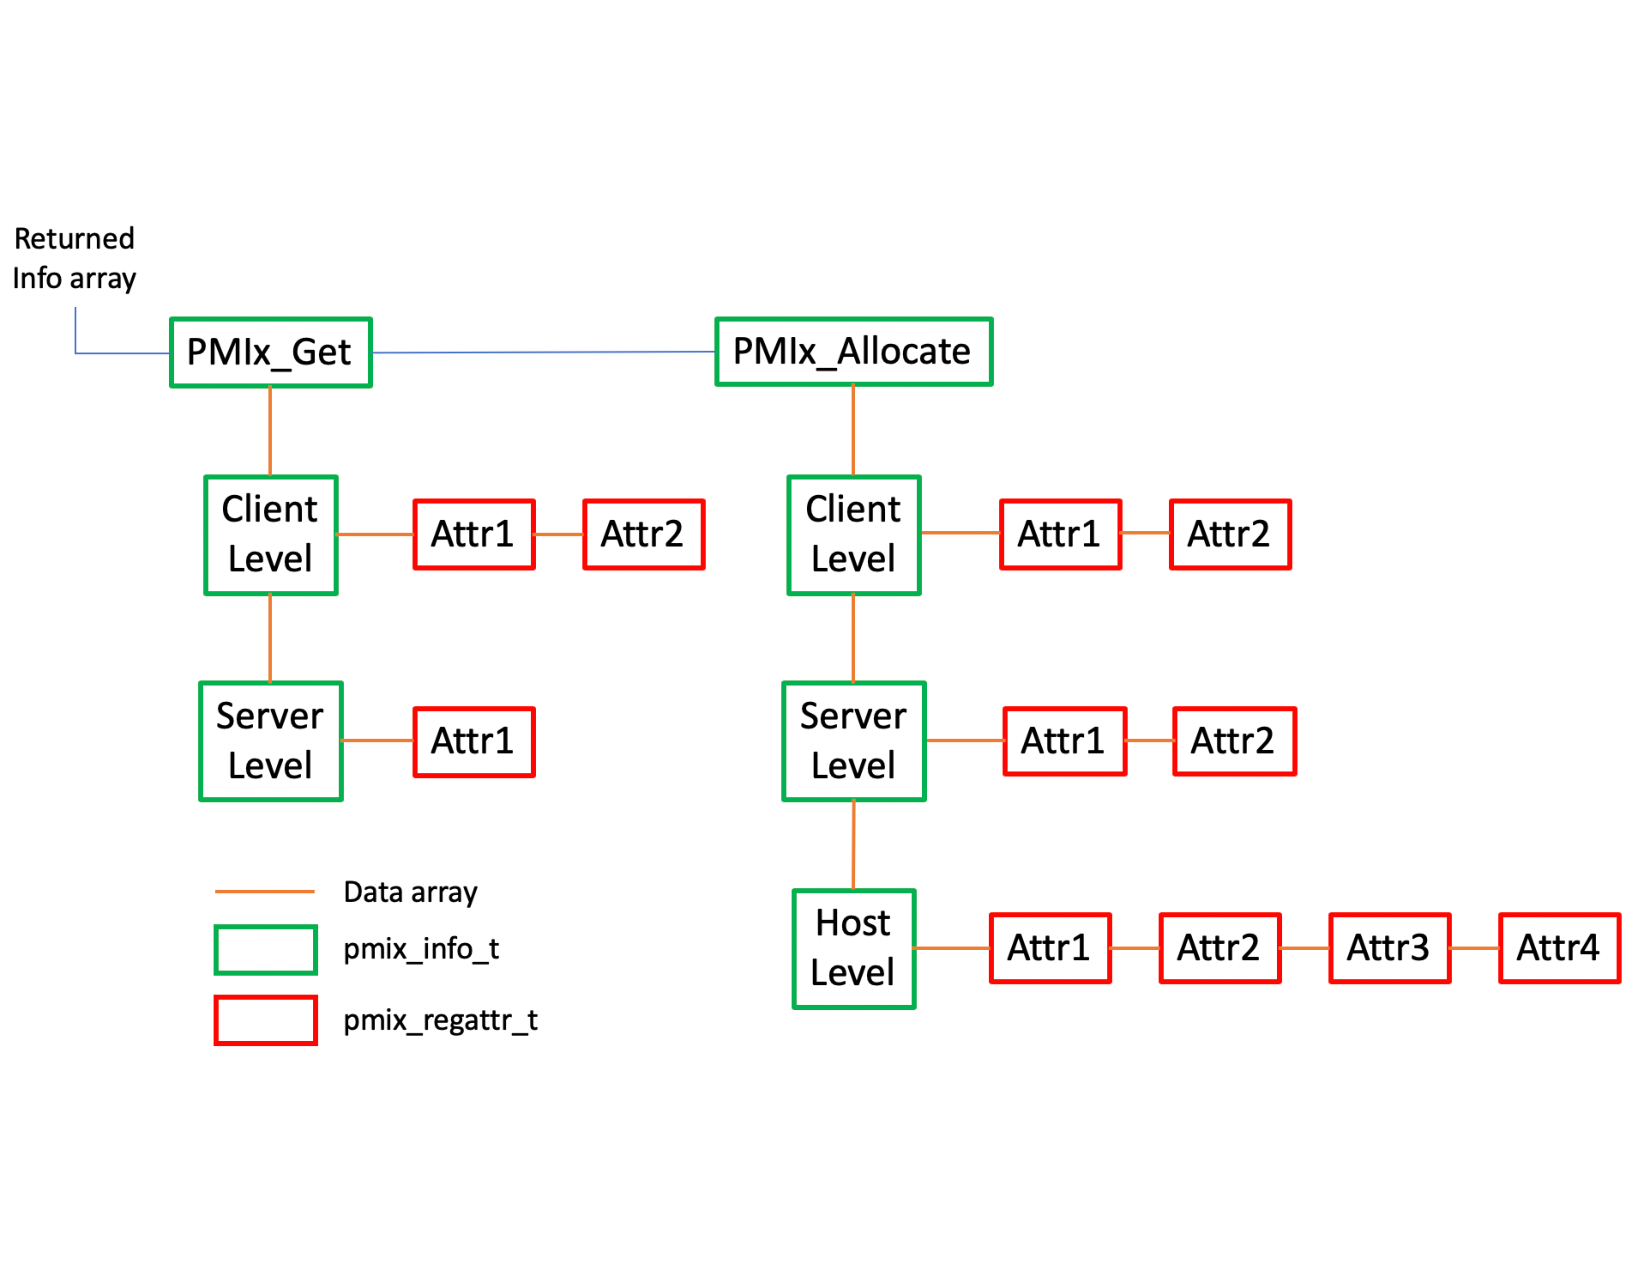
\includegraphics[clip,width=0.8\textwidth]{figs/attrquery.pdf}
  \end{center}
  \caption{Returned information hierarchy for attribute support request}
  \label{fig:attrquery}
\end{figure*}
\endgroup

The array of returned structures, and their child arrays, are subject to the return rules for the \refapi{PMIx_Query_info_nb} \ac{API}. For example, a request for supported attributes of the \refapi{PMIx_Get} function that includes the \refarg{host} level will return values for the \refarg{client} and \refarg{server} levels, plus an array element with a \refarg{key} of \refattr{PMIX_HOST_ATTRIBUTES} and a value type of \refconst{PMIX_UNDEF} indicating that no attributes are supported at that level.

%%%%%%%%%%%%%%%%%%%%%%%%%%%%%%%%%%%%%%%%%%%%%%%%%

    %%%%%%%%%%%%%%%%%%%%%%%%%%%%%%%%%%%%%%%%%%%%%%%%%
% Chapter: Synchronization
%%%%%%%%%%%%%%%%%%%%%%%%%%%%%%%%%%%%%%%%%%%%%%%%%
\chapter{Synchronization}
\label{chap:api_sync}

Applications may need to synchronize their operations at various points in
their execution. Depending on a variety of factors (e.g., the programming
model and where the synchronization point lies), the application may choose to
execute the operation using \ac{PMIx} to access the communication capabilities
of the host environment's infrastructure. This is particularly useful in
situations where communication libraries are not yet initialized by the application.
Synchronization operations also offer an opportunity for processes to exchange
data at a known point in their execution.  For example, communication libraries within
different processes can synchronize to exchange information on communication endpoints
for subsequent wireup of messaging protocols.

\ac{PMIx} clients can use the \refapi{PMIx_Fence} and \refapi{PMIx_Fence_nb} functions
to synchronize a set of processes.  The fence operation can be useful after an application
performs a number of \refapi{PMIx_Put} operations to coordinate with other processes that the
data is available for access.   This avoids unsuccessful \refapi{PMIx_Get} calls that might
otherwise be invoked before the cooresponding \refapi{PMIx_Put} call is complete.

In its default form, the fence operation acts as a barrier between the processes and does not exchange data.
Clients can pass the \refattr{PMIX_COLLECT_DATA} attribute to request
that the \refapi{PMIx_Fence} and \refapi{PMIx_Fence_nb} functions exchange all committed
data between all involved servers during the synchronization operation.
This will make local to each process the data put by other processes resulting
in faster resolution of \refapi{PMIx_Get} and \refapi{PMIx_Get_nb} function calls at
the cost of a synchronous data exchange and associated memory footprint expansion.
In many situations
this attribute may have performance benefits as many systems are optimized for transporting
larger amounts of data.  In such applications, a 'put/commit/fence/get'
pattern is common for efficiently exchanging key-value pairs.
For applications where only a small subset of clients access another small subset's key-value pairs
this attribute may not be beneficial.  As such, applications are not required to use
\refapi{PMIx_Fence} or \refapi{PMIx_Fence_nb} functions nor the associated data collection
attribute to ensure correctness of \ac{PMIx} get/put functionality.

%%%%%%%%%%%%%%%%%%%%%%%%%%%%%%%%%%%%%%%%%%%%%%%%%
%%%%%%%%%%%%%%%%%%%%%%%%%%%%%%%%%%%%%%%%%%%%%%%%%
\section{\code{PMIx_Fence}}
\declareapi{PMIx_Fence}

%%%%
\summary

Execute a blocking barrier across the processes identified in the specified array, collecting information posted via \refapi{PMIx_Put} as directed.

%%%%
\format

\copySignature{PMIx_Fence}{1.0}{
pmix_status_t \\
PMIx_Fence(const pmix_proc_t procs[], size_t nprocs, \\
\hspace*{11\sigspace}const pmix_info_t info[], size_t ninfo);
}

\begin{arglist}
\argin{procs}{Array of \refstruct{pmix_proc_t} structures (array of handles)}
\argin{nprocs}{Number of elements in the \refarg{procs} array (integer)}
\argin{info}{Array of info structures (array of handles)}
\argin{ninfo}{Number of elements in the \refarg{info} array (integer)}
\end{arglist}

\returnsimple

\reqattrstart
The following attributes are required to be supported by all \ac{PMIx} libraries:

\pasteAttributeItem{PMIX_COLLECT_DATA}
\pasteAttributeItem{PMIX_COLLECT_GENERATED_JOB_INFO}

\reqattrend

\optattrstart
The following attributes are optional for \ac{PMIx} implementations:

\pasteAttributeItem{PMIX_ALL_CLONES_PARTICIPATE}


The following attributes are optional for host environments:

\pasteAttributeItem{PMIX_TIMEOUT}

\optattrend

%%%%
\descr

Passing a \code{NULL} pointer as the \refarg{procs} parameter indicates that the fence is to span all processes in the client's namespace.
Each provided \refstruct{pmix_proc_t} struct can pass \refconst{PMIX_RANK_WILDCARD} to indicate that all processes in the given namespace are participating.
The ordering of the entries in the \refarg{procs} has no significance.  However, all processes engaged in a given
\refapi{PMIx_Fence}
operation must use the same method to identify processes.  Callers which describe
the target set of processes using PMIX_RANK_WILDCARD will not be matched with
callers which list the individual processes of a namespace explicitly.

The \refarg{info} array is used to pass user directives regarding the behavior of the fence operation. Note that for scalability reasons, the default behavior for \refapi{PMIx_Fence} is to not collect data posted by the operation's participants.

\adviceimplstart
\refapi{PMIx_Fence} and its non-blocking form are both \emph{collective} operations. Accordingly, the \ac{PMIx} server library is required to aggregate participation by local clients, passing the request to the host environment once all local participants have executed the \ac{API}.
\adviceimplend

\advicermstart
The host will receive a single call for each collective operation. It is the responsibility of the host to identify the nodes containing participating processes, execute the collective across all participating nodes, and notify the local \ac{PMIx} server library upon completion of the global collective.
\advicermend


%%%%%%%%%%%%%%%%%%%%%%%%%%%%%%%%%%%%%%%%%%%%%%%%%
%%%%%%%%%%%%%%%%%%%%%%%%%%%%%%%%%%%%%%%%%%%%%%%%%
\section{\code{PMIx_Fence_nb}}
\declareapi{PMIx_Fence_nb}

%%%%
\summary

Execute a nonblocking \refapi{PMIx_Fence} across the processes identified in the specified array of processes, collecting information posted via \refapi{PMIx_Put} as directed.

%%%%
\format

\copySignature{PMIx_Fence_nb}{1.0}{
pmix_status_t \\
PMIx_Fence_nb(const pmix_proc_t procs[], size_t nprocs, \\
\hspace*{14\sigspace}const pmix_info_t info[], size_t ninfo, \\
\hspace*{14\sigspace}pmix_op_cbfunc_t cbfunc, void *cbdata);
}

\begin{arglist}
\argin{procs}{Array of \refstruct{pmix_proc_t} structures (array of handles)}
\argin{nprocs}{Number of elements in the \refarg{procs} array (integer)}
\argin{info}{Array of info structures (array of handles)}
\argin{ninfo}{Number of elements in the \refarg{info} array (integer)}
\argin{cbfunc}{Callback function (function reference)}
\argin{cbdata}{Data to be passed to the callback function (memory reference)}
\end{arglist}

\returnsimplenb

\returnstart
\begin{itemize}
    \item \refconst{PMIX_OPERATION_SUCCEEDED}, indicating that the request was immediately processed and returned \textit{success} - the \refarg{cbfunc} will \textit{not} be called. This can occur if the collective involved only processes on the local node.
\end{itemize}
\returnend

\reqattrstart
The following attributes are required to be supported by all \ac{PMIx} libraries:

\pasteAttributeItem{PMIX_COLLECT_DATA}
\pasteAttributeItem{PMIX_COLLECT_GENERATED_JOB_INFO}

\reqattrend

\optattrstart
The following attributes are optional for \ac{PMIx} implementations:

\pasteAttributeItem{PMIX_ALL_CLONES_PARTICIPATE}


The following attributes are optional for host environments that support this operation:

\pasteAttributeItem{PMIX_TIMEOUT}

\optattrend

%%%%
\descr

Nonblocking version of the \refapi{PMIx_Fence} routine. See the \refapi{PMIx_Fence} description for further details.

%%%%%%%%%%%%%%%%%%%%%%%%%%%%%%%%%%%%%%%%%%%%%%%%%
\subsection{Fence-related attributes}

The following attributes are defined specifically to support the fence operation:

%
\declareAttribute{PMIX_COLLECT_DATA}{"pmix.collect"}{bool}{
Collect all data posted by the participants using \refapi{PMIx_Put} that
has been committed via \refapi{PMIx_Commit}, making the collection locally
available to each participant at the end of the operation. By default, this will include all job-level information that was locally generated by \ac{PMIx} servers unless excluded using the \refattr{PMIX_COLLECT_GENERATED_JOB_INFO} attribute.
}

\declareAttribute{PMIX_LOCAL_COLLECTIVE_STATUS}{"pmix.loc.col.st"}{pmix_status_t}{
Status code for local collective operation being reported to the host by the server library. PMIx servers may aggregate the participation by local client processes in a collective operation - e.g., instead of passing individual client calls to \refapi{PMIx_Fence} up to the host environment, the server may pass only a single call to the host when all local participants have executed their \refapi{PMIx_Fence} call, thereby reducing the burden placed on the host. However, in cases where the operation locally fails (e.g., if a participating client abnormally terminates prior to calling the operation), the server upcall functions to the host do not include a \refstruct{pmix_status_t} by which the PMIx server can alert the host to that failure. This attribute resolves that problem by allowing the server to pass the status information regarding the local collective operation.
}
\advicermstart
The PMIx server is allowed to pass \refconst{PMIX_SUCCESS} using this attribute, but is not required to do so. PMIx implementations may choose to only report errors in this manner. The lack of an included status shall therefore be taken to indicate that the collective operation locally succeeded.
\advicermend
%
\declareAttribute{PMIX_COLLECT_GENERATED_JOB_INFO}{"pmix.collect.gen"}{bool}{
Collect all job-level information (i.e., reserved keys) that was locally generated by \ac{PMIx} servers. Some job-level information (e.g., distance between processes and fabric devices) is best determined on a distributed basis as it primarily pertains to local processes. Should remote processes need to access the information, it can either be obtained collectively using the \refapi{PMIx_Fence} operation with this directive, or can be retrieved one peer at a time using \refapi{PMIx_Get} without first having performed the job-wide collection.
}
%
\declareAttribute{PMIX_ALL_CLONES_PARTICIPATE}{"pmix.clone.part"}{bool}{
All \refterm{clones} of the calling process must participate in the collective operation.
}


%%%%%%%%%%%%%%%%%%%%%%%%%%%%%%%%%%%%%%%%%%%%%%%%%

    %%%%%%%%%%%%%%%%%%%%%%%%%%%%%%%%%%%%%%%%%%%%%%%%%
% Chapter: Publish/Lookup Operations
%%%%%%%%%%%%%%%%%%%%%%%%%%%%%%%%%%%%%%%%%%%%%%%%%
\chapter{Publish/Lookup Operations}
\label{chap:pub}

Chapter~\ref{chap:api_rsvd_keys}
and
Section ~\ref{chap:data_sharing:non_rsvd_keys}
present how reserved and non-reserved keys deal with
information that either is associated with a specific process (i.e., the
retrieving process knows the identifier of the process that posted it) or
requires a synchronization operation prior to retrieval (e.g., the case of
globally unique non-reserved keys). However, another requirement exists for an
asynchronous exchange of data where neither the posting nor the retrieving
process is known in advance (e.g. two namespaces that do not share a child-parent relationship).
The \acp{API} defined in this section focus on resolving that specific
situation by allowing processes to publish data that can subsequently be
retrieved solely by referral to its key. Mechanisms for constraining
the scope of availability of the information are also provided as a means for better
targeting of the eventual recipient(s).

Note that no presumption is made regarding how the published information is to be stored, nor as to the entity (host environment or \ac{PMIx} implementation) that shall act as the datastore. The descriptions in the remainder of this chapter shall simply refer to that entity as the \emph{datastore}.

%%%%%%%%%%%%%%%%%%%%%%%%%%%%%%%%%%%%%%%%%%%%%%%%%
%%%%%%%%%%%%%%%%%%%%%%%%%%%%%%%%%%%%%%%%%%%%%%%%%
\section{\code{PMIx_Publish_datastore}}

\declareapiProvisional{PMIx_Publish_datastore}

%%%%
\summary

Publish data for later access via \refapi{PMIx_Lookup_datastore}.

%%%%
\format


\cspecificstart
\begin{codepar}
pmix_status_t \\
PMIx_Publish_datastore(const pmix_info_t pinfo[], size_t npinfo, \\
\hspace*{12\sigspace}pmix_publish_id_t *publish_id, \\
\hspace*{12\sigspace}const pmix_info_t info[], size_t ninfo);
\end{codepar}
\cspecificend

\begin{arglist}
\argin{pinfo}{Array of key value pairs to publish (array of \refstruct{pmix_info_t})}
\argin{npinfo}{Number of elements in the \refarg{pinfo} array (integer)}
\argout{publish_id}{The location to store a publish_id used to uniquely identify this call}
\argin{info}{Array of info structures (array of \refstruct{pmix_info_t})}
\argin{ninfo}{Number of elements in the \refarg{info} array (integer)}
\end{arglist}
%
\returnsimple
%
\reqattrstart
There are no required attributes for this \ac{API}. \ac{PMIx} implementations that do not directly support the operation but are hosted by environments that do support it must pass any attributes that are provided by the client to the host environment for processing. In addition, the \ac{PMIx} library is required to add the \refAttributeItem{PMIX_USERID} and the \refAttributeItem{PMIX_GRPID} attributes of the client process that published the information to the \refarg{info} array passed to the host environment.
\reqattrend

\optattrstart
The following attributes are optional for host environments that support this operation:

\pasteAttributeItem{PMIX_TIMEOUT}
\pasteAttributeItem{PMIX_RANGE}
\pasteAttributeItem{PMIX_PERSISTENCE}
\pasteAttributeItem{PMIX_ACCESS_USERIDS}
\pasteAttributeItem{PMIX_ACCESS_GRPIDS}
\pasteAttributeItem{PMIX_ACCESS_PERMISSIONS}

\optattrend

%%%%
\descr

Publish the data in the \refarg{pinfo} array for subsequent lookup.
By default, data is accessible by all processes in the same session as the publisher.  
The attributes \refconst{PMIX_RANGE}, 
\refAttributeItem{PMIX_ACCESS_USERIDS}, \refAttributeItem{PMIX_ACCESS_GRPIDS} and \refAttributeItem{PMIX_ACCESS_PERMISSIONS} 
can be included in the \refarg{info} array to restrict the processes that can access the published data on systems 
which support these attributes.  
By default, the data will remain published until
all processes in the publishing application terminate.  The attribute \refconst{PMIX_PERSISTENCE} 
can be included in the \refarg{info} array to change if and when data will be automatically 
unpublished for systems which support this attribute (See Section \ref{chap:pub:types:persist})

Each published key is assigned a epoch number when it is published to help identify the relative order
that value assignments are made to a key when a key is assigned multiple values.
All of the keys in the \refarg{pinfo} array will be associated with the same epoch number.  
Within a single process, each call to \refapi{PMIx_Publish_datastore} or \refapi{PMIx_Publish_datastore_nb}
will return a unique value.   
If one call to \refapi{PMIx_Publish_datastore} or \refapi{PMIx_Publish_datastore_nb} returns successfully before 
another call to either \ac{API} is initiated by a process,
the former should assign a smaller epoch number than the 
later call.  In the case where two calls by processes on the same host overlap in time, 
the implementation should make a best effort to determine which call was made first and assign the 
keys of that call a smaller epoch number.  
A key with a greater epoch number be never be visible to other processes before a key with 
a lesser epoch number.

\adviceuserstart
To ensure that one call to \refapi{PMIx_Publish_datastore} call is assigned a smaller value than another 
call across multiple threads or processes it may be necessary to use synchronization primatives. 
\refapi{PMIx_Fence} is a \ac{PMIx} \ac{API} that can be used for synchronizing across multiple processes.
\adviceuserend

\adviceimplstart
The requirement for an implementation to assign an epoch number permits a variety of implementations.  If a centeralized 
datastore is used, the epoch number can be a simple epoch number such as a counter that is incremented on each
\refapi{PMIx_Publish_datastore} and \refapi{PMIx_Publish_datastore_nb} call.  Alternatively, the epoch number can
be a time value if hosts are guaranteed to have clocks with sufficient resolution and synchronization to ensure
that consecutive calls can be distiguished as occuring at different points of time.
\adviceimplend

The returned \refarg{publish_id} is used to associate the published key values with the specific publish
call used to publish them.  A \refstruct{pmix_publish_id_t} can be used to determine the publishing
process (\refstruct{pmix_proc_t}) and the epoch number of a call to publish data.. 
The \refarg{publish_epoch} must be retained for unpublishing and may be transfered to other processes 
either for unpublishing or to uniquely identify a specific value of a key.

The blocking form of this call will block until it has obtained confirmation from the datastore that the data is available for lookup. 
The \refarg{pinfo} array can be released upon return from the blocking function call.

Clients performing a lookup operation with \refapi{PMIx_Lookup_datastore} on
a key will
receive a list of all accessible values published for that key.  The lookup \acp{API} also allows the caller to further
restrict what values are considered accessible, such as restricting which publishing processes to consider.

%%%%%%%%%%%%%%%%%%%%%%%%%%%%%%%%%%%%%%%%%%%%%%%%%
%%%%%%%%%%%%%%%%%%%%%%%%%%%%%%%%%%%%%%%%%%%%%%%%%
\section{\code{PMIx_Publish_datastore_nb}}

\declareapiProvisional{PMIx_Publish_datastore_nb}

%%%%
\summary

Nonblocking \refapi{PMIx_Publish_datastore} routine.

%%%%
\format

\cspecificstart
\begin{codepar}
pmix_status_t \\
PMIx_Publish_datastore_nb(const pmix_info_t pinfo[], size_t npinfo, \\
\hspace*{12\sigspace}const pmix_info_t info[], size_t ninfo, \\
\hspace*{16\sigspace}pmix_publish_datastore_cbfunc_t cbfunc, void *cbdata);
\end{codepar}
\cspecificend

\begin{arglist}
\argin{pinfo}{Array of key value pairs to publish (array of \refstruct{pmix_info_t})}
\argin{npinfo}{Number of elements in the \refarg{pinfo} array (integer)}
\argin{info}{Array of info structures (array of \refstruct{pmix_info_t})}
\argin{ninfo}{Number of elements in the \refarg{info} array (integer)}
\argin{cbfunc}{Callback function \refapi{pmix_publish_datastore_cbfunc_t} (function reference)}
\argin{cbdata}{Data to be passed to the callback function (memory reference)}
\end{arglist}

\returnsimplenb

\reqattrstart
There are no required attributes for this \ac{API}. \ac{PMIx} implementations that do not directly support the operation but are hosted by environments that do support it must pass any attributes that are provided by the client to the host environment for processing. In addition, the \ac{PMIx} library is required to add the \refAttributeItem{PMIX_USERID} and the \refAttributeItem{PMIX_GRPID} attributes of the client process that published the information to the \refarg{info} array passed to the host environment.
\reqattrend

\optattrstart
The following attributes are optional for host environments that support this operation:

\pasteAttributeItem{PMIX_TIMEOUT}
\pasteAttributeItem{PMIX_RANGE}
\pasteAttributeItem{PMIX_PERSISTENCE}
\pasteAttributeItem{PMIX_ACCESS_USERIDS}
\pasteAttributeItem{PMIX_ACCESS_GRPIDS}
\pasteAttributeItem{PMIX_ACCESS_PERMISSIONS}

\optattrend

%%%%
\descr

Nonblocking \refapi{PMIx_Publish_datastore} routine.  The handle to the published data is returned 
as a parameter to the callback function during a successful call.

%%%%%%%%%%%%%%%%%%%%%%%%%%%%%%%%%%%%%%%%%%%%%%%%%
\section{\code{PMIx_Lookup_datastore}}
\declareapiProvisional{PMIx_Lookup_datastore}

%%%%
\summary

Lookup information published by a process or host environment using \refapi{PMIx_Publish_datastore} or \refapi{PMIx_Publish_datastore_nb}.

%%%%
\format

\cspecificstart
\begin{codepar}
pmix_status_t \\
PMIx_Lookup_datastore(pmix_key_t keys[], \\
\hspace*{12\sigspace}pmix_pdsdata_t data[], \\  
\hspace*{12\sigspace}size_t nkeys_and_data, \\
\hspace*{12\sigspace}const pmix_info_t info[], \\
\hspace*{12\sigspace}size_t ninfo);
\end{codepar}
\cspecificend

\begin{arglist}
\argin{keys}{array of keys (array of strings)}
\arginout{data}{Array of \refstruct{pmix_pdsdata_t} structures providing storage for the results. (array of \refstruct{pmix_pdsdata_t})}
\argin{nkeys_and_data}{Number of elements in the \refarg{keys} and \refarg{data} arrays (integer)}
\argin{info}{Array of info structures (array of handles)}
\argin{ninfo}{Number of elements in the \refarg{info} array (integer)}
\end{arglist}

\returnstart
\begin{itemize}
\item \refconst{PMIX_ERR_NOT_FOUND} None of the requested data could be found within the requester's range.  The address pointed to by \refarg{nresults} will be set to 0.

\item \refconst{PMIX_ERR_PARTIAL_SUCCESS} Some of the requested data was found.  
Any key that cannot be found will return with a data type of \refconst{PMIX_UNDEF} in the associated \refarg{value} struct. Note that the specific reason for a particular piece of missing information (e.g., lack of permissions) cannot be communicated back to the requester in this situation.
Only found data will be included in the returned \refarg{data} array. Note that the specific reason for a particular piece of missing information (e.g., lack of permissions or the data has not been published) cannot be communicated back to the requester in this situation.

\end{itemize}
\returnend

\reqattrstart
\ac{PMIx} libraries are not required to directly support any attributes for this function. However, any provided attributes must be passed to the host environment for processing, and the \ac{PMIx} library is required to add the \refAttributeItem{PMIX_USERID} and the \refAttributeItem{PMIX_GRPID} attributes of the client process that is requesting the info.

\reqattrend

\optattrstart
The following attributes are optional for host environments that support this operation:

\pasteAttributeItem{PMIX_TIMEOUT}
\pasteAttributeItem{PMIX_RANGE}
\pasteAttributeItem{PMIX_WAIT}

\optattrend

%%%%
\descr

Lookup information published by a process or host environment using \refapi{PMIx_Publish_datastore} 
or \refapi{PMIx_Publish_datastore_nb}.
A lookup operation is always performed on a range which can be specified using the directive \refAttributeItem{PMIX_RANGE} or otherwise defaults to \refconst{PMIX_RANGE_SESSION}.

The lookup operation will be constrained to data published to the specified range.
Data is returned per the retrieval rules of Section \ref{chap:pub:retrules}.

The \argref{key} parameter consists of an array of \refstruct{pmix_key_t} structures specifying the requested information.
The \argref{data} parameter provides space for the results.  The operation will fill in each 
\argref{data} structure's key field with the corresponding key in the \argref{key} array. 
The \code{value} and \code{publish_id} fields will be filled in with the results of the lookup operation.
The length of the \code{publish_id} and \code{value} data arrays will be the number of published values matching the requested
key and may be 0.  The \code{value} field of \refstruct{pmix_data_array_t} will contain \refstruct{pmix_value_t} elements and will have its \code{type} field set to \refconst{PMIX_VALUE}.
The \code{publish_id} field of \refstruct{pmix_data_array_t} will contain \refstruct{pmix_publish_id_t} elements 
and will have its \code{type} field set to \refconst{PMIX_PUBLISH_ID}.

\adviceuserstart
Although this is a blocking function, it will not wait by default for the requested data to be published.
Instead, it will block for the time required by the datastore to lookup its current data and return any found items.
Thus, the caller is responsible for either ensuring that data is published prior to executing a lookup, using \refattr{PMIX_WAIT} to instruct the datastore to wait for the data to be published, or retrying until the requested data is found.
\adviceuserend


%%%%%%%%%%%%%%%%%%%%%%%%%%%%%%%%%%%%%%%%%%%%%%%%%
%%%%%%%%%%%%%%%%%%%%%%%%%%%%%%%%%%%%%%%%%%%%%%%%%
\section{\code{PMIx_Lookup_datastore_nb}}
\declareapi{PMIx_Lookup_datastore_nb}

%%%%
\summary

Nonblocking version of \refapi{PMIx_Lookup_datastore}.

%%%%
\format

\cspecificstart
\begin{codepar}
pmix_status_t \\
PMIx_Lookup_datastore_nb(pmix_key_t keys[], \\
\hspace*{15\sigspace}size_t nkeys, \\
\hspace*{15\sigspace}const pmix_info_t info[], size_t ninfo, \\
\hspace*{15\sigspace}pmix_lookup_datastore_cbfunc_t cbfunc, void *cbdata);
\end{codepar}
\cspecificend

\begin{arglist}
\argin{keys}{array of keys (array of strings)}
\argin{nkeys}{Number of elements in the \refarg{keys} array (integer)}
\argin{info}{Array of info structures (array of handles)}
\argin{ninfo}{Number of elements in the \refarg{info} array (integer)}
\argin{cbfunc}{Callback function \refapi{pmix_lookup_datastore_cbfunc_t} (function reference)}
\argin{cbdata}{Callback data to be provided to the callback function (pointer)}
\end{arglist}

\returnsimplenb

If executed, the status returned in the provided callback function will be one of the following constants:

\begin{itemize}
\item \refconst{PMIX_SUCCESS} All data was found and has been returned.

\item \refconst{PMIX_ERR_NOT_FOUND} None of the requested data was available within the requester's range. The \refarg{pdata} array in the callback function shall be \code{NULL} and the \refarg{npdata} parameter set to zero.

\item \refconst{PMIX_ERR_PARTIAL_SUCCESS} Some of the requested data was found.
Only found data will be included in the returned \refarg{pdata} array. Note that the specific reason for a particular piece of missing information (e.g., lack of permissions or the data has not been published) cannot be communicated back to the requester in this situation.

\item \refconst{PMIX_ERR_NOT_SUPPORTED} There is no available datastore (either at the host environment or \ac{PMIx} implementation level) on this system that supports this function.

\item \refconst{PMIX_ERR_NO_PERMISSIONS} All of the requested data was found and range restrictions were met for each specified key, but none of the matching data could be returned due to lack of access permissions.

\item a non-zero \ac{PMIx} error constant indicating a reason for the request's failure.
\end{itemize}

\reqattrstart
\ac{PMIx} libraries are not required to directly support any attributes for this function. However, any provided attributes must be passed to the host environment for processing, and the \ac{PMIx} library is required to add the \refAttributeItem{PMIX_USERID} and the \refAttributeItem{PMIX_GRPID} attributes of the client process that is requesting the info.

\reqattrend

\optattrstart
The following attributes are optional for host environments that support this operation:

\pasteAttributeItem{PMIX_TIMEOUT}
\pasteAttributeItem{PMIX_RANGE}
\pasteAttributeItem{PMIX_WAIT}

\optattrend

%%%%
\descr

Non-blocking form of the \refapi{PMIx_Lookup_datastore} function.  The \refapi{pmix_lookup_datastore_cbfunc_t} 
will be called on successful completion and will provide available values for the requested keys.

%%%%%%%%%%%%%%%%%%%%%%%%%%%%%%%%%%%%%%%%%%%%%%%%%
\section{\code{PMIx_Unpublish_datastore}}
\declareapiProvisional{PMIx_Unpublish_datastore}

%%%%
\summary

Unpublish a list of keys published by the calling process using \refapi{PMIx_Publish_datastore}.

% TODO: Define PMIX_PUBLISH_IDLEN.
% TODO: Do we want something like PMIX_PUBLISH_ID_ALL_MINE (like PMIX_PUBLISH_ID_ALL, but only for caller)
% TODO: Create API to translate a publish-id to a proc + epoch number
% TODO: macro's for creating/freeing pmix_pdsdata_t's
% TODO: Discuss how lookup values are released freed (these are arrays of values for each key and they
are allocated by the system)
% TODO: lookup blocking and non-blocking are so different.  Should we separate keys from return values in the 
blocking call so it looks more like the non-blocking call.

%%%%
\format

\cspecificstart
\begin{codepar}
pmix_status_t \\
PMIx_Unpublish_datastore(const pmix_key_t keys_to_unpublish[], \\
\hspace*{15\sigspace}const pmix_publish_id_t publish_id[], \\
\hspace*{15\sigspace}size_t nkeys, \\
\hspace*{15\sigspace}const pmix_info_t info[], size_t ninfo);
\end{codepar}
\cspecificend

\begin{arglist}
\argin{keys_to_unpublish}{Array of keys to unpublish (array of handles)}
\argin{publish_id}{Array of publish identifiers indicating the publishing call that published the corresponding entry in \refarg{keys_to_unpublish} (array of handles)}
\argin{nkeys}{Number of elements in the \refarg{keys_to_unpublish} and \refarg{publish_id} keys}
\argin{info}{Array of info structures (array of handles)}
\argin{ninfo}{Number of elements in the \refarg{info} array (integer)}
\end{arglist}

\returnsimple

\reqattrstart
\ac{PMIx} libraries are not required to directly support any attributes for this function. However, any provided attributes must be passed to the host environment for processing, and the \ac{PMIx} library is required to add the \refAttributeItem{PMIX_USERID} and the \refAttributeItem{PMIX_GRPID} attributes of the client process that is requesting the operation.

\reqattrend

\optattrstart
The following attributes are optional for host environments that support this operation:

\pasteAttributeItem{PMIX_TIMEOUT}
\pasteAttributeItem{PMIX_RANGE}

\optattrend

%%%%
\descr

Unpublish a list of keys published by the calling process using \refapi{PMIx_Publish_datastore}.
The function will block until the data has been removed by the server (i.e., it keys associated with the handle are no longer visible to to other processes).  Passing \code{NULL} for a key in \refarg{keys_to_unpublish} indicates that the 
call should unpublish all keys that have been published by the corresponding publish identifier in 
\refarg{publish_id}.
A value of \refconst{PMIX_PUBLISH_ID_ALL} may be used for the \refarg{publish_id} for a key to indicate that the value should 
be unpublished for any and all previous publish calls for which the caller has permission to unpublish.  This includes the calling process or any other process running as the same user.  

%%%%%%%%%%%%%%%%%%%%%%%%%%%%%%%%%%%%%%%%%%%%%%%%%
%%%%%%%%%%%%%%%%%%%%%%%%%%%%%%%%%%%%%%%%%%%%%%%%%
\section{\code{PMIx_Unpublish_datastore_nb}}
\declareapiProvisional{PMIx_Unpublish_datastore_nb}

%%%%
\summary

Nonblocking version of \refapi{PMIx_Unpublish_datastore}.

%%%%
\format

\cspecificstart
\begin{codepar}
pmix_status_t \\
PMIx_Unpublish_datastore_nb(const pmix_key_t keys_to_unpublish[], \\
\hspace*{15\sigspace}const pmix_publish_id_t publish_id[], \\
\hspace*{15\sigspace}size_t nkeys, \\
\hspace*{15\sigspace}const pmix_info_t info[], size_t ninfo, \\
\hspace*{18\sigspace}pmix_op_cbfunc_t cbfunc, void *cbdata);
\end{codepar}
\cspecificend

\begin{arglist}
\argin{keys_to_unpublish}{Array of keys to unpublish (array of handles)}
\argin{publish_id}{Array of publish identifiers indicating the publishing call that published the corresponding entry in \refarg{keys_to_unpublish} (array of handles)}
\argin{nkeys}{Number of elements in the \refarg{keys_to_unpublish} and \refarg{publish_id} keys}
\argin{info}{Array of info structures (array of handles)}
\argin{ninfo}{Number of elements in the \refarg{info} array (integer)}
\argin{cbfunc}{Callback function \refapi{pmix_op_cbfunc_t} (function reference)}
\argin{cbdata}{Data to be passed to the callback function (memory reference)}
\end{arglist}

\returnsimplenb

\returnstart
\begin{itemize}
    \item \refconst{PMIX_OPERATION_SUCCEEDED}, indicating that the request was immediately processed and returned \textit{success} - the \refarg{cbfunc} will \textit{not} be called.
\end{itemize}
\returnend

\reqattrstart
\ac{PMIx} libraries are not required to directly support any attributes for this function. However, any provided attributes must be passed to the host environment for processing, and the \ac{PMIx} library is required to add the \refAttributeItem{PMIX_USERID} and the \refAttributeItem{PMIX_GRPID} attributes of the client process that is requesting the operation.

\reqattrend

\optattrstart
The following attributes are optional for host environments that support this operation:

\pasteAttributeItem{PMIX_TIMEOUT}

\optattrend

%%%%
\descr

Non-blocking form of the \refapi{PMIx_Unpublish} function.
The callback function will be executed once the server confirms removal of the specified data. The \refarg{info} array must be maintained until the callback is provided.


%%%%%%%%%%%%%%%%%%%%%%%%%%%%%%%%%%%%%%%%%%%%%%%%%

%%%%%%%%%%%%%%%%%%%%%%%%%%%%%%%%%%%%%%%%%%%%%%%%%
%%%%%%%%%%%%%%%%%%%%%%%%%%%%%%%%%%%%%%%%%%%%%%%%%
\section{\code{PMIx_Publish}}
\declareapi{PMIx_Publish}

%%%%
\summary

Publish data for later access via \refapi{PMIx_Lookup}.

%%%%
\format

\copySignature{PMIx_Publish}{1.0}{
pmix_status_t \\
PMIx_Publish(const pmix_info_t info[], size_t ninfo);
}

\begin{arglist}
\argin{info}{Array of info structures containing both data to be published and directives (array of handles)}
%% (array of handles is used everywhere, but it is not really an array of handles, so I'm not sure why)
\argin{ninfo}{Number of elements in the \refarg{info} array (integer)}
\end{arglist}

\returnsimple

\reqattrstart
There are no required attributes for this \ac{API}. \ac{PMIx} implementations that do not directly support the operation but are hosted by environments that do support it must pass any attributes that are provided by the client to the host environment for processing. In addition, the \ac{PMIx} library is required to add the \refAttributeItem{PMIX_USERID} and the \refAttributeItem{PMIX_GRPID} attributes of the client process that published the information to the \refarg{info} array passed to the host environment.

\reqattrend

\optattrstart
The following attributes are optional for host environments that support this operation:

\pasteAttributeItem{PMIX_TIMEOUT}
\pasteAttributeItem{PMIX_RANGE}
\pasteAttributeItem{PMIX_PERSISTENCE}
\pasteAttributeItem{PMIX_ACCESS_USERIDS}
\pasteAttributeItem{PMIX_ACCESS_GRPIDS}
\pasteAttributeItem{PMIX_ACCESS_PERMISSIONS}

\optattrend

%%%%
\descr

Publish the data in the \refarg{info} array for subsequent lookup.
By default, the data will be published into the \refconst{PMIX_RANGE_SESSION} range and with \refconst{PMIX_PERSIST_APP} persistence.
Changes to those values, and any additional directives, can be included in the \refstruct{pmix_info_t} array. Attempts to access the data by processes outside of the provided data range shall be rejected. The \refattr{PMIX_PERSISTENCE} attribute instructs the datastore holding the published information as to how long that information is to be retained.

The blocking form of this call will block until it has obtained confirmation from the datastore that the data is available for lookup. The \refarg{info} array can be released upon return from the blocking function call.

Publishing duplicate keys is permitted provided they are published to different
ranges. Custom ranges are considered different if they have different members.
Duplicate keys being published on the same data range shall return the
\refconst{PMIX_ERR_DUPLICATE_KEY} error.

%In some cases, implementations may be incapable of distinguishing which
%info keys in the \refarg{info} array are for publishing and which info keys are
%directives.  To make it clear, it is recommended that the keys to be published
%are designated by passing them as a \refstruct{pmix_data_array_t} using the
%\refattr{PMIX_DATA_TO_PUBLISH} directive.
%If the \refarg{info} array contains a \refattr{PMIX_DATA_TO_PUBLISH} info,
%all other elements of the info array will be treated as directives.
%If the info array does not include a \refattr{PMIX_DATA_TO_PUBLISH} info,
%the implementation should
%distinguish between info array elements that specify keys and directives as follows:
%All standardized directives to the publish call,
%including optional attributes the implementation does not support,
%should be treated as
%directives.  Non-supported directives
%may be ignored as outlined in Section \ref{intro:portability:attributes},
%but should not be treated as data to
%publish.  The implementation may treat any custom (non-standardized) directives it
%supports as directives.  All other \refarg{info} array elements
%should be assumed to be data to be published.
%Since additional directives may be added to the standard and implementations may add support for additional custom directives, the use of \refattr{PMIX_DATA_TO_PUBLISH} is the only reliable way to ensure that
%future implementations will not mis-classify elements of an \refarg{info} array.

%%%%%%%%%%%%%%%%%%%%%%%%%%%%%%%%%%%%%%%%%%%%%%%%%
%%%%%%%%%%%%%%%%%%%%%%%%%%%%%%%%%%%%%%%%%%%%%%%%%
\section{\code{PMIx_Publish_nb}}

\declareapi{PMIx_Publish_nb}

%%%%
\summary

Nonblocking \refapi{PMIx_Publish} routine.

%%%%
\format

\copySignature{PMIx_Publish_nb}{1.0}{
pmix_status_t \\
PMIx_Publish_nb(const pmix_info_t info[], size_t ninfo, \\
\hspace*{16\sigspace}pmix_op_cbfunc_t cbfunc, void *cbdata);
}

\begin{arglist}
\argin{info}{Array of info structures containing both data to be published and directives (array of handles)}
\argin{ninfo}{Number of elements in the \refarg{info} array (integer)}
\argin{cbfunc}{Callback function \refapi{pmix_op_cbfunc_t} (function reference)}
\argin{cbdata}{Data to be passed to the callback function (memory reference)}
\end{arglist}

\returnsimplenb

\returnstart
\begin{itemize}
    \item \refconst{PMIX_OPERATION_SUCCEEDED}, indicating that the request was immediately processed and returned \textit{success} - the \refarg{cbfunc} will \textit{not} be called.
\end{itemize}
\returnend

\reqattrstart
There are no required attributes for this \ac{API}. \ac{PMIx} implementations that do not directly support the operation but are hosted by environments that do support it must pass any attributes that are provided by the client to the host environment for processing. In addition, the \ac{PMIx} library is required to add the \refAttributeItem{PMIX_USERID} and the \refAttributeItem{PMIX_GRPID} attributes of the client process that published the information to the \refarg{info} array passed to the host environment.
\reqattrend

\optattrstart
The following attributes are optional for host environments that support this operation:

\pasteAttributeItem{PMIX_TIMEOUT}
\pasteAttributeItem{PMIX_RANGE}
\pasteAttributeItem{PMIX_PERSISTENCE}
\pasteAttributeItem{PMIX_ACCESS_USERIDS}
\pasteAttributeItem{PMIX_ACCESS_GRPIDS}
\pasteAttributeItem{PMIX_ACCESS_PERMISSIONS}

\optattrend

%%%%
\descr

Nonblocking \refapi{PMIx_Publish} routine.


%%%%%%%%%%%%%%%%%%%%%%%%%%%%%%%%%%%%%%%%%%%%%%%%%
%%%%%%%%%%%%%%%%%%%%%%%%%%%%%%%%%%%%%%%%%%%%%%%%%
\section{Publish-specific constants}

The following constants are defined for use with the \refapi{PMIx_Publish} \acp{API}:

\begin{constantdesc}
%
\declareconstitemvalue{PMIX_ERR_DUPLICATE_KEY}{-53}
The provided key has already been published on the same data range.
%
\end{constantdesc}

%%The following constants are defined for use with the \refapi{PMIx_Publish_datastore} \acp{API}:

\versionMarkerProvisional{5.0}
\begin{constantdesc}
%
\declareconstitemvalueNEW{PMIX_PUBLISH_ID_ALL}{0...0}
A constant \refstruct{pmix_publish_id_t} indicating all successful publish datastore operations made by calling process.
%
\end{constantdesc}

%%%%%%%%%%%%%%%%%%%%%%%%%%%%%%%%%%%%%%%%%%%%%%%%%
%%%%%%%%%%%%%%%%%%%%%%%%%%%%%%%%%%%%%%%%%%%%%%%%%
\section{Publish-specific attributes}

The following attributes are defined for use with the \refapi{PMIx_Publish} \acp{API}:

%
\declareAttribute{PMIX_RANGE}{"pmix.range"}{pmix_data_range_t}{
Define constraints on the processes that can access published data or generated events or define constraints on the provider of data when looking up published data.
}
%
\declareAttribute{PMIX_PERSISTENCE}{"pmix.persist"}{pmix_persistence_t}{
Declare how long the datastore shall retain the provided data. The datastore is to delete the data upon reaching the persistence criterion.
}
%
\declareAttribute{PMIX_ACCESS_PERMISSIONS}{"pmix.aperms"}{pmix_data_array_t}{
Define access permissions for the published data. The value shall contain an array of \refstruct{pmix_info_t} structs containing the specified permissions.
}
%
\declareAttribute{PMIX_ACCESS_USERIDS}{"pmix.auids"}{pmix_data_array_t}{
Array of effective \acp{UID} that are allowed to access the published data.
}
%
\declareAttribute{PMIX_ACCESS_GRPIDS}{"pmix.agids"}{pmix_data_array_t}{
Array of effective \acp{GID} that are allowed to access the published data.
}
%

%%%%%%%%%%%%%%%%%%%%%%%%%%%%%%%%%%%%%%%%%%%%%%%%%
%%%%%%%%%%%%%%%%%%%%%%%%%%%%%%%%%%%%%%%%%%%%%%%%%
\section{Publish-Lookup Datatypes}

The following data types are defined for use with the \refapi{PMIx_Publish} \acp{API}.

%%%%%%%%%%%%%%%%%%%%%%%%%%%%%%%%%%%%%%%%%%%%%%%%%

\subsection{Publisher Identifier}
\versionMarkerProvisional{5.0}
\declarestruct{pmix_publish_epoch_t}
The \refstruct{pmix_publish_epoch_t} structure is a is a \code{uint64_t} type for identifying a publish epoch.

\versionMarkerProvisional{5.0}
\declarestruct{pmix_publish_id_t}
The \refstruct{pmix_publish_id_t} structure is a statically defined character array of length
PMIX_PUBLISH_IDLEN. 
The structure is an opaque object from the perspective of the client.
An implementation is responsible for storing sufficient information within the structure to identify 
a specific call to \refapi{PMIx_Publish_datastore} or \refapi{PMIx_Publish_datastore_nb} within the system.

\adviceimplstart
An implementation may simply embed a \refstruct{pmix_proc_t} and a \refstruct{pmix_publish_epoch_t} within 
the storage provided by \refstruct{pmix_publish_id_t}.  However, implementations are free to optimize the
use of this space to allow for faster lookup or to support publish/lookup operations across sessions.
\adviceimplend

\subsection{Range of Published Data}
\declarestruct{pmix_data_range_t}

\versionMarker{1.0}
The \refstruct{pmix_data_range_t} structure is a \code{uint8_t} type that defines a range for data \textit{published} via the \refapi{PMIx_Publish} \ac{API} and events generated via the \refapi{PMIx_Notify_event}.
The following constants can be used to set a variable of the type \refstruct{pmix_data_range_t}.

\begin{constantdesc}
%
\declareconstitemvalue{PMIX_RANGE_UNDEF}{0}
Undefined range.
%
\declareconstitemvalue{PMIX_RANGE_RM}{1}
Data is intended for the host environment, or lookup is restricted to data published by the host environment.
%
\declareconstitemvalue{PMIX_RANGE_LOCAL}{2}
Published data and generated events are restricted to processes on the same node as the publisher or event creator.  Lookup of data is restricted to data published by processes on the same node as the requester.
%
\declareconstitemvalue{PMIX_RANGE_NAMESPACE}{3}
Published data and generated events are restricted to processes in the same namespace as the publisher or event creator.
Lookup of data is restricted to data published by procesess in the same namespace as the requester.
%
\declareconstitemvalue{PMIX_RANGE_SESSION}{4}
Published data and generated events are restricted to processes in the same session as the publisher or event creator.
Lookup of data is restricted to data published by procesess in the same session as the requester.
%
\declareconstitemvalue{PMIX_RANGE_GLOBAL}{5}
Published data and generated events are available to all processes within the domain of the host environment.
Lookup of data is unrestricted and open to data published by any processes within the domain of the host enivornment as the requester.  This range differs from \refconst{PMIX_RANGE_RM} only on systems which have mechanisms to share events and
publish/lookup data across multiple instances of a host environment.
%
\declareconstitemvalue{PMIX_RANGE_PROC_LOCAL}{7}
Published data and generated events are available only to calling process.
Lookup of data is restricted to data published by the calling process.
%
\declareconstitemvalue{PMIX_RANGE_CUSTOM}{6}
Published data and generated events are restricted to processes
described in the \refstruct{pmix_info_t} associated with this call.
Lookup of data is restricted to data published by the processes described in
in the \refstruct{pmix_info_t}.
%
\declareconstitemvalue{PMIX_RANGE_INVALID}{UINT8_MAX}
Invalid value - typically used to indicate that a range has not yet been set.
%
\end{constantdesc}


%%%%%%%%%%%%%%%%%%%%%%%%%%%%%%%%%%%%%%%%%%%%%%%%%
\subsection{Data Persistence Structure}
\label{chap:pub:types:persist}
\declarestruct{pmix_persistence_t}

\versionMarker{1.0}
The \refstruct{pmix_persistence_t} structure is a \code{uint8_t} type that defines the policy for data published by clients via the \refapi{PMIx_Publish} \ac{API}.
The following constants can be used to set a variable of the type \refstruct{pmix_persistence_t}.

\begin{constantdesc}
%
\declareconstitemvalue{PMIX_PERSIST_INDEF}{0}
Retain data until unpublished.
%
\declareconstitemvalue{PMIX_PERSIST_FIRST_READ}{1}
Retain data until the first access, then the data is deleted.
%
\declareconstitemvalue{PMIX_PERSIST_PROC}{2}
Retain data until the publishing process terminates.
%
\declareconstitemvalue{PMIX_PERSIST_APP}{3}
Retain data until the application terminates.
%
\declareconstitemvalue{PMIX_PERSIST_SESSION}{4}
Retain data until the session/allocation terminates.
%
\declareconstitemvalue{PMIX_PERSIST_INVALID}{UINT8_MAX}
Invalid value - typically used to indicate that a persistence has not yet been set.
%
\end{constantdesc}


%%%%%%%%%%%%%%%%%%%%%%%%%%%%%%%%%%%%%%%%%%%%%%%%%
\subsection{Lookup Related Data Structures}

\declarestruct{pmix_pdata_t}

The \refstruct{pmix_pdata_t} structure is used both to request the lookup of keys and to describe the value and publishing process of any keys that were successfully retrieved.
A request to lookup published values is described by an array of \refstruct{pmix_pdata_t} structures.
Only the key field is used in the lookup request.
The results of the lookup operation are returned in the same array with the proc and value fields set when the key is successfully found.
The value field's data type is set to \refconst{PMIX_UNDEF} in the associated \refarg{value} struct of any key which was not retrieved.
%
\copySignature{pmix_pdata_t}{1.0}{
typedef struct pmix_pdata \{ \\
\hspace*{4\sigspace}pmix_proc_t proc; \\
\hspace*{4\sigspace}pmix_key_t key; \\
\hspace*{4\sigspace}pmix_value_t value; \\
\} pmix_pdata_t;
}

where:
\begin{itemize}
    \item \emph{proc} is the process identifier of the data publisher.
    \item \emph{key} is the string key of the published data.
    \item \emph{value} is the value associated with the \emph{key}.
\end{itemize}

\declarestruct{pmix_pdsdata_t}

The \refstruct{pmix_pdsdata_t} structure is used both to request the lookup of keys and to describe the value and publishing process of any keys that were successfully retrieved.
A request to lookup published values is described by an array of \refstruct{pmix_pdsdata_t} structures.
Only the key field is used in the lookup request.
The results of the lookup operation are returned in the same array with the proc and value fields set when the key is successfully found.
The value field's data type is set to \refconst{PMIX_UNDEF} in the associated \refarg{value} struct of any key which was not retrieved.
%
\copySignature{pmix_pdsdata_t}{5.0}{
typedef struct pmix_pdsdata \{ \\
\hspace*{4\sigspace}pmix_key_t key; \\
\hspace*{4\sigspace}pmix_data_array_t value; \\
\hspace*{4\sigspace}pmix_data_array_t publish_id; \\
\} pmix_pdata_t;
}

where:

\begin{itemize}
    \item \emph{key} is the string key of the published data.
    \item \emph{value} is a pmix data array of values that have been published for the key 
    \item \emph{publish_id} is a pmix data array of the same length as the \refarg{value} array containing the 
    identifier of the publish call that created the value.
    \item \emph{value} is the value associated with the \emph{key}.
\end{itemize}

%%%%%%%%%%%%%%%%%%%%%%%%%%%%%%%%%%%%%%%%%%%%%%%%%
%%%%%%%%%%%%%%%%%%%%%%%%%%%%%%%%%%%%%%%%%%%%%%%%%
\section{\code{PMIx_Lookup}}
\declareapi{PMIx_Lookup}

%%%%
\summary

Lookup information published by a process or host environment using \refapi{PMIx_Publish} or \refapi{PMIx_Publish_nb}.

%%%%
\format

\copySignature{PMIx_Lookup}{1.0}{
pmix_status_t \\
PMIx_Lookup(pmix_pdata_t data[], size_t ndata, \\
\hspace*{12\sigspace}const pmix_info_t info[], size_t ninfo);
}

\begin{arglist}
\arginout{data}{Array of publishable data structures (array of \refstruct{pmix_pdata_t})}
\argin{ndata}{Number of elements in the \refarg{data} array (integer)}
\argin{info}{Array of info structures (array of \refstruct{pmix_info_t})}
\argin{ninfo}{Number of elements in the \refarg{info} array (integer)}
\end{arglist}

\returnstart
\begin{itemize}
\item \refconst{PMIX_ERR_NOT_FOUND} None of the requested data could be found within the requester's range.

\item \refconst{PMIX_ERR_PARTIAL_SUCCESS} Some of the requested data was found.
Any key that cannot be found will return with a data type of \refconst{PMIX_UNDEF} in the associated \refarg{value} struct. Note that the specific reason for a particular piece of missing information (e.g., lack of permissions) cannot be communicated back to the requester in this situation.

\item \refconst{PMIX_ERR_NO_PERMISSIONS} All requested data was found and range restrictions were met for each specified key, but none of the matching data could be returned due to lack of access permissions.

\end{itemize}
\returnend

\reqattrstart
\ac{PMIx} libraries are not required to directly support any attributes for this function. However, any provided attributes must be passed to the host environment for processing, and the \ac{PMIx} library is required to add the \refAttributeItem{PMIX_USERID} and the \refAttributeItem{PMIX_GRPID} attributes of the client process that is requesting the info.

\reqattrend

\optattrstart
The following attributes are optional for host environments that support this operation:

\pasteAttributeItem{PMIX_TIMEOUT}
\pasteAttributeItem{PMIX_RANGE}
\pasteAttributeItem{PMIX_WAIT}

\optattrend

%%%%
\descr

Lookup information published by a process or host environment using \refapi{PMIx_Publish} or \refapi{PMIx_Publish_nb}.
A lookup operation is always performed on a range which can be specified using the directive \refAttributeItem{PMIX_RANGE} or otherwise defaults to \refconst{PMIX_RANGE_SESSION}.

The lookup operation will be constrained to data published to the specified range.
Data is returned per the retrieval rules of Section \ref{chap:pub:retrules}.

The \argref{data} parameter consists of an array of \refstruct{pmix_pdata_t} structures with the keys specifying the requested information.
Data will be returned for each \code{key} field in the associated \code{value} field of this structure as per the above description of return values. The \code{proc} field in each \refstruct{pmix_pdata_t} structure will contain the namespace/rank of the process that published the data.

\adviceuserstart
Although this is a blocking function, it will not wait by default for the requested data to be published.
Instead, it will block for the time required by the datastore to lookup its current data and return any found items.
Thus, the caller is responsible for either ensuring that data is published prior to executing a lookup, using \refattr{PMIX_WAIT} to instruct the datastore to wait for the data to be published, or retrying until the requested data is found.
\adviceuserend


%%%%%%%%%%%%%%%%%%%%%%%%%%%%%%%%%%%%%%%%%%%%%%%%%
%%%%%%%%%%%%%%%%%%%%%%%%%%%%%%%%%%%%%%%%%%%%%%%%%
\section{\code{PMIx_Lookup_nb}}
\declareapi{PMIx_Lookup_nb}

%%%%
\summary

Nonblocking version of \refapi{PMIx_Lookup}.

%%%%
\format

\copySignature{PMIx_Lookup_nb}{1.0}{
pmix_status_t \\
PMIx_Lookup_nb(char **keys, \\
\hspace*{15\sigspace}const pmix_info_t info[], size_t ninfo, \\
\hspace*{15\sigspace}pmix_lookup_cbfunc_t cbfunc, void *cbdata);
}

\begin{arglist}
\argin{keys}{\code{NULL}-terminated array of keys (array of strings)}
\argin{info}{Array of info structures (array of handles)}
\argin{ninfo}{Number of elements in the \refarg{info} array (integer)}
\argin{cbfunc}{Callback function \refapi{pmix_lookup_cbfunc_t} (function reference)}
\argin{cbdata}{Callback data to be provided to the callback function (pointer)}
\end{arglist}

\returnsimplenb

If executed, the status returned in the provided callback function will be one of the following constants:

\begin{itemize}
\item \refconst{PMIX_SUCCESS} All data was found and has been returned.

\item \refconst{PMIX_ERR_NOT_FOUND} None of the requested data was available within the requester's range. The \refarg{pdata} array in the callback function shall be \code{NULL} and the \refarg{npdata} parameter set to zero.

\item \refconst{PMIX_ERR_PARTIAL_SUCCESS} Some of the requested data was found.
Only found data will be included in the returned \refarg{pdata} array. Note that the specific reason for a particular piece of missing information (e.g., lack of permissions or the data has not been published) cannot be communicated back to the requester in this situation.

\item \refconst{PMIX_ERR_NOT_SUPPORTED} There is no available datastore (either at the host environment or \ac{PMIx} implementation level) on this system that supports this function.

\item \refconst{PMIX_ERR_NO_PERMISSIONS} All of the requested data was found and range restrictions were met for each specified key, but none of the matching data could be returned due to lack of access permissions.

\item a non-zero \ac{PMIx} error constant indicating a reason for the request's failure.
\end{itemize}

\reqattrstart
\ac{PMIx} libraries are not required to directly support any attributes for this function. However, any provided attributes must be passed to the host environment for processing, and the \ac{PMIx} library is required to add the \refAttributeItem{PMIX_USERID} and the \refAttributeItem{PMIX_GRPID} attributes of the client process that is requesting the info.

\reqattrend

\optattrstart
The following attributes are optional for host environments that support this operation:

\pasteAttributeItem{PMIX_TIMEOUT}
\pasteAttributeItem{PMIX_RANGE}
\pasteAttributeItem{PMIX_WAIT}

\optattrend

%%%%
\descr

Non-blocking form of the \refapi{PMIx_Lookup} function.

%%%%%%%%%%%%%%%%%%%%%%%%%%%%%%%%%%%%%%%%%%%%%%%%%
\subsubsection{Lookup data structure support macros}

The following macros are provided to support the \refstruct{pmix_pdata_t} structure.

%%%%
\littleheader{Static initializer for the pdata structure}
\declaremacroProvisional{PMIX_LOOKUP_STATIC_INIT}

Provide a static initializer for the \refstruct{pmix_pdata_t} fields.

\versionMarker{5.0}
\cspecificstart
\begin{codepar}
PMIX_LOOKUP_STATIC_INIT
\end{codepar}
\cspecificend


\littleheader{Initialize the pdata structure}
\declaremacro{PMIX_PDATA_CONSTRUCT}

Initialize the \refstruct{pmix_pdata_t} fields

\copySignature{PMIX_PDATA_CONSTRUCT}{1.0}{
PMIX_PDATA_CONSTRUCT(m)
}

\begin{arglist}
\argin{m}{Pointer to the structure to be initialized (pointer to \refstruct{pmix_pdata_t})}
\end{arglist}

\littleheader{Destruct the pdata structure}
\declaremacro{PMIX_PDATA_DESTRUCT}

Destruct the \refstruct{pmix_pdata_t} fields

\copySignature{PMIX_PDATA_DESTRUCT}{1.0}{
PMIX_PDATA_DESTRUCT(m)
}

\begin{arglist}
\argin{m}{Pointer to the structure to be destructed (pointer to \refstruct{pmix_pdata_t})}
\end{arglist}

%%%%%%%%%%%
\littleheader{Create a pdata array}
\declaremacro{PMIX_PDATA_CREATE}

Allocate and initialize an array of \refstruct{pmix_pdata_t} structures

\copySignature{PMIX_PDATA_CREATE}{1.0}{
PMIX_PDATA_CREATE(m, n)
}

\begin{arglist}
\arginout{m}{Address where the pointer to the array of \refstruct{pmix_pdata_t} structures shall be stored (handle)}
\argin{n}{Number of structures to be allocated (\code{size_t})}
\end{arglist}


%%%%%%%%%%%
\littleheader{Free a pdata structure}
\declaremacro{PMIX_PDATA_RELEASE}

Release a \refstruct{pmix_pdata_t} structure

\copySignature{PMIX_PDATA_RELEASE}{4.0}{
PMIX_PDATA_RELEASE(m)
}

\begin{arglist}
\argin{m}{Pointer to a \refstruct{pmix_pdata_t} structure (handle)}
\end{arglist}


%%%%%%%%%%%
\littleheader{Free a pdata array}
\declaremacro{PMIX_PDATA_FREE}

Release an array of \refstruct{pmix_pdata_t} structures

\copySignature{PMIX_PDATA_FREE}{1.0}{
PMIX_PDATA_FREE(m, n)
}

\begin{arglist}
\argin{m}{Pointer to the array of \refstruct{pmix_pdata_t} structures (handle)}
\argin{n}{Number of structures in the array (\code{size_t})}
\end{arglist}

%%%%%%%%%%%
\littleheader{Load a lookup data structure}
\declaremacro{PMIX_PDATA_LOAD}

This macro simplifies the loading of key, process identifier, and data into a \refstruct{pmix_pdata_t} by correctly assigning values to the structure's fields.

\copySignature{PMIX_PDATA_LOAD}{1.0}{
PMIX_PDATA_LOAD(m, p, k, d, t);
}

\begin{arglist}
\argin{m}{Pointer to the \refstruct{pmix_pdata_t} structure into which the key and data are to be loaded (pointer to \refstruct{pmix_pdata_t})}
\argin{p}{Pointer to the \refstruct{pmix_proc_t} structure containing the identifier of the process being referenced (pointer to \refstruct{pmix_proc_t})}
\argin{k}{String key to be loaded - must be less than or equal to \refconst{PMIX_MAX_KEYLEN} in length (handle)}
\argin{d}{Pointer to the data value to be loaded (handle)}
\argin{t}{Type of the provided data value (\refstruct{pmix_data_type_t})}
\end{arglist}

\adviceuserstart
Key, process identifier, and data will all be copied into the \refstruct{pmix_pdata_t} - thus, the source information can be modified or free'd without affecting the copied data once the macro has completed.
\adviceuserend

%%%%%%%%%%%
\littleheader{Transfer a lookup data structure}
\declaremacro{PMIX_PDATA_XFER}

This macro simplifies the transfer of key, process identifier, and data value between two\refstruct{pmix_pdata_t} structures.

\copySignature{PMIX_PDATA_XFER}{2.0}{
PMIX_PDATA_XFER(d, s);
}

\begin{arglist}
\argin{d}{Pointer to the destination \refstruct{pmix_pdata_t} (pointer to \refstruct{pmix_pdata_t})}
\argin{s}{Pointer to the source \refstruct{pmix_pdata_t} (pointer to \refstruct{pmix_pdata_t})}
\end{arglist}

\adviceuserstart
Key, process identifier, and data will all be copied into the destination \refstruct{pmix_pdata_t} - thus, the source \refstruct{pmix_pdata_t} may free'd without affecting the copied data once the macro has completed.
\adviceuserend

%%%%%%%%%%%%%%%%%%%%%%%%%%%%%%%%%%%%%%%%%%%%%%%%%
\section{Retrieval rules for published data}
\label{chap:pub:retrules}

The retrieval rules for published data primarily revolve around enforcing data access permissions and range constraints.
All publish and lookup operations operate on a range. If not specified, the range defaults to \refconst{PMIX_RANGE_SESSION}.
The key being looked up will match with a published key only if all of the following conditions are met:

\begin{enumerate}
    \item The lookup key matches the published key.
    \item The type of range specified by the publisher is the same as the type of range specified by the requester.
    \item The requestor must be a member of the range specified by the publisher.
    \item The publisher must be a member of the range specified by the requestor.
    \item If the publisher specified access permissions, the effective \ac{UID} and \ac{GID} of the requester must meet those requirements.
\end{enumerate}

The status returned by the datastore shall be set to:

\begin{itemize}
\item \refconst{PMIX_SUCCESS} All data was found and is included in the returned information.

\item \refconst{PMIX_ERR_NOT_FOUND} None of the requested data could be found within a requester's range.

\item \refconst{PMIX_ERR_PARTIAL_SUCCESS} Some of the requested data was found.
Only found data will be included in the returned information. Note that the specific reason for a particular piece of missing information (e.g., lack of permissions) cannot be communicated back to the requester in this situation.

\item \refconst {PMIX_ERR_NO_PERMISSIONS} All requested data was found and range restrictions were met for each specified key, but none of the matching data could be returned due to lack of access permissions.

\item a non-zero \ac{PMIx} error constant indicating a reason for the request's failure.
\end{itemize}

%%%%%%%%%%%%%%%%%%%%%%%%%%%%%%%%%%%%%%%%%%%%%%%%%
%%%%%%%%%%%%%%%%%%%%%%%%%%%%%%%%%%%%%%%%%%%%%%%%%
\section{\code{PMIx_Unpublish}}
\declareapi{PMIx_Unpublish}

%%%%
\summary

Unpublish a list of keys published by the calling process.

%%%%
\format

\copySignature{PMIx_Unpublish}{1.0}{
pmix_status_t \\
PMIx_Unpublish(char **keys, \\
\hspace*{15\sigspace}const pmix_info_t info[], size_t ninfo);
}

\begin{arglist}
\argin{keys}{\code{NULL}-terminated array of keys (array of strings)}
\argin{info}{Array of info structures (array of handles)}
\argin{ninfo}{Number of elements in the \refarg{info} array (integer)}
\end{arglist}

\returnsimple

\reqattrstart
\ac{PMIx} libraries are not required to directly support any attributes for this function. However, any provided attributes must be passed to the host environment for processing, and the \ac{PMIx} library is required to add the \refAttributeItem{PMIX_USERID} and the \refAttributeItem{PMIX_GRPID} attributes of the client process that is requesting the operation.

\reqattrend

\optattrstart
The following attributes are optional for host environments that support this operation:

\pasteAttributeItem{PMIX_TIMEOUT}
\pasteAttributeItem{PMIX_RANGE}

\optattrend

%%%%
\descr

Unpublish a list of keys published by the calling process.
The function will block until the data has been removed by the server (i.e., it is safe to publish that key again within the specified range).
A value of \code{NULL} for the \refarg{keys} parameter instructs the server to remove all data published by this process.

By default, the range is assumed to be \refconst{PMIX_RANGE_SESSION}.
Changes to the range, and any additional directives, can be provided in the \refarg{info} array.


%%%%%%%%%%%%%%%%%%%%%%%%%%%%%%%%%%%%%%%%%%%%%%%%%
%%%%%%%%%%%%%%%%%%%%%%%%%%%%%%%%%%%%%%%%%%%%%%%%%
\section{\code{PMIx_Unpublish_nb}}
\declareapi{PMIx_Unpublish_nb}

%%%%
\summary

Nonblocking version of \refapi{PMIx_Unpublish}.

%%%%
\format

\copySignature{PMIx_Unpublish_nb}{1.0}{
pmix_status_t \\
PMIx_Unpublish_nb(char **keys, \\
\hspace*{18\sigspace}const pmix_info_t info[], size_t ninfo, \\
\hspace*{18\sigspace}pmix_op_cbfunc_t cbfunc, void *cbdata);
}

\begin{arglist}
\argin{keys}{\code{NULL}-terminated array of keys (array of strings)}
\argin{info}{Array of info structures (array of handles)}
\argin{ninfo}{Number of elements in the \refarg{info} array (integer)}
\argin{cbfunc}{Callback function \refapi{pmix_op_cbfunc_t} (function reference)}
\argin{cbdata}{Data to be passed to the callback function (memory reference)}
\end{arglist}

\returnsimplenb

\returnstart
\begin{itemize}
    \item \refconst{PMIX_OPERATION_SUCCEEDED}, indicating that the request was immediately processed and returned \textit{success} - the \refarg{cbfunc} will \textit{not} be called.
\end{itemize}
\returnend

\reqattrstart
\ac{PMIx} libraries are not required to directly support any attributes for this function. However, any provided attributes must be passed to the host environment for processing, and the \ac{PMIx} library is required to add the \refAttributeItem{PMIX_USERID} and the \refAttributeItem{PMIX_GRPID} attributes of the client process that is requesting the operation.

\reqattrend

\optattrstart
The following attributes are optional for host environments that support this operation:

\pasteAttributeItem{PMIX_TIMEOUT}
\pasteAttributeItem{PMIX_RANGE}

\optattrend

%%%%
\descr

Non-blocking form of the \refapi{PMIx_Unpublish} function.
The callback function will be executed once the server confirms removal of the specified data. The \refarg{info} array must be maintained until the callback is provided.


%%%%%%%%%%%%%%%%%%%%%%%%%%%%%%%%%%%%%%%%%%%%%%%%%


    % Event Handling
    %  - (de)register_event, notify_event
    %%%%%%%%%%%%%%%%%%%%%%%%%%%%%%%%%%%%%%%%%%%%%%%%%
% Chapter: Events
%%%%%%%%%%%%%%%%%%%%%%%%%%%%%%%%%%%%%%%%%%%%%%%%%
\chapter{Event Notification}
\label{chap:api_event}

This chapter defines the \ac{PMIx} event notification system.
These interfaces are designed to support the reporting of events to/from clients and servers, and between library layers within a single process.

%%%%%%%%%%%%%%%%%%%%%%%%%%%%%%%%%%%%%%%%%%%%%%%%%
%%%%%%%%%%%%%%%%%%%%%%%%%%%%%%%%%%%%%%%%%%%%%%%%%
\section{Notification and Management}
\label{chap:api_event:notify}

\ac{PMIx} event notification provides an asynchronous out-of-band mechanism for communicating events between application processes and/or elements of the \ac{SMS}. Its uses span a wide range including fault notification, coordination between multiple programming libraries within a single process, and workflow orchestration for non-synchronous programming models. Events can be divided into two distinct classes:

\begin{itemize}
\item \textit{Job-specific events} directly relate to a job executing within the session, such as a debugger attachment, process failure within a related job, or events generated by an application process. Events in this category are to be immediately delivered to the \ac{PMIx} server library for relay to the related local processes.

\item \textit{Environment events} indirectly relate to a job but do not specifically target the job itself. This category includes \ac{SMS}-generated events such as \ac{ECC} errors, temperature excursions, and other non-job conditions that might directly affect a session's resources, but would never include an event generated by an application process. Note that although these do potentially impact the session's jobs, they are not directly tied to those jobs. Thus, events in this category are to be delivered to the \ac{PMIx} server library only upon request.
\end{itemize}

Both \ac{SMS} elements and applications can register for events of either type.

\adviceimplstart
Race conditions can cause the registration to come after events of possible interest (e.g., a memory \ac{ECC} event that occurs after start of execution but prior to registration, or an application process generating an event prior to another process registering to receive it). \ac{SMS} vendors are \textit{requested} to cache environment events for some time to mitigate this situation, but are not \textit{required} to do so. However, \ac{PMIx} implementers are \textit{required} to cache all events received by the \ac{PMIx} server library and to deliver them to registering clients in the same order in which they were received.
\adviceimplend

\adviceuserstart
Applications must be aware that they may not receive environment events that occur prior to registration, depending upon the capabilities of the host \ac{SMS}.
\adviceuserend

The generator of an event can specify the \textit{target range} for delivery of that event. Thus, the generator can choose to limit notification to processes on the local node, processes within the same job as the generator, processes within the same allocation, other threads within the same process, only the \ac{SMS} (i.e., not to any application processes), all application processes, or to a custom range based on specific process identifiers. Only processes within the given range that register for the provided event code will be notified. In addition, the generator can use attributes to direct that the event not be delivered to any default event handlers, or to any multi-code handler (as defined below).

Event notifications provide the process identifier of the source of the event plus the event code and any additional information provided by the generator. When an event notification is received by a process, the registered handlers are scanned for their event code(s), with matching handlers assembled into an \textit{event chain} for servicing. Note that users can also specify a \textit{source range} when registering an event (using the same range designators described above) to further limit when they are to be invoked. When assembled, the PMIx event chain is ordered based on both the specificity of the event handler and user directives at time of handler registration. By default, handlers are grouped into three categories based on the number of event codes that can trigger the callback:
\begin{itemize}
%
\item \textit{single-code} handlers are serviced first as they are the most specific. These are handlers that are registered against one specific event code.
%
\item \textit{multi-code} handlers are serviced once all single-code handlers have completed. The handler will be included in the chain upon receipt of an event matching any of the provided codes.
%
\item \textit{default} handlers are serviced once all multi-code handlers have completed. These handlers are always included in the chain unless the generator specifically excludes them.
%
\end{itemize}

Users can specify the callback order of a handler within its category at the time of registration. 
Users can specify that a given handler be executed before or after another target handler should both handlers appear in an event chain (the ordering is ignored if the other handler isn't included). 
The ordering is dictated by providing the event handler name of the target.  The name must have been assigned the target handler was registered.
Note that ordering does not imply immediate relationships. For example, multiple handlers registered to be serviced after event handler \textit{A} will all be executed after \textit{A}, but are not guaranteed to be executed in any particular order amongst themselves.

In addition, one event handler can be declared as the \textit{first} handler to be executed in the chain. This handler will \textit{always} be called prior to any other handler, regardless of category, provided the incoming event matches both the specified range and event code. Only one handler can be so designated --- attempts to designate additional handlers as \textit{first} will return an error. Deregistration of the declared \textit{first} handler will re-open the position for subsequent assignment.

Similarly, one event handler can be declared as the \textit{last} handler to be executed in the chain. This handler will \textit{always} be called after all other handlers have executed, regardless of category, provided the incoming event matches both the specified range and event code. Note that this handler will not be called if the chain is terminated by an earlier handler. Only one handler can be designated as \textit{last} --- attempts to designate additional handlers as \textit{last} will return an error. Deregistration of the declared \textit{last} handler will re-open the position for subsequent assignment.

\adviceuserstart
Note that the \textit{last} handler is called \textit{after} all registered default handlers that match the specified range of the incoming event unless a handler prior to it terminates the chain. Thus, if the application intends to define a \textit{last} handler, it should ensure that no default handler aborts the process before it.
\adviceuserend

Upon completing its work and prior to returning, each handler \textit{must} call the event handler completion function provided when it was invoked (including a status code plus any information to be passed to later handlers) so that the chain can continue being progressed. \ac{PMIx} automatically aggregates the status and any results of each handler (as provided in the completion callback) with status from all prior handlers so that each step in the chain has full knowledge of what preceded it. An event handler can terminate all further progress along the chain by passing the \refconst{PMIX_EVENT_ACTION_COMPLETE} status to the completion callback function.

\subsection{Events versus status constants}
\label{api:event:evssc}

Return status constants (see Section \ref{api:struct:errors}) represent values that can be returned from or passed into \ac{PMIx}
\acp{API}. These are distinct from \ac{PMIx} \emph{events} in that they are
not values that can be registered against event handlers. In general, the two
types of constants are distinguished by inclusion of an "ERR" in the name of
error constants versus an "EVENT" in events, though there are exceptions (e.g,
the \refconst{PMIX_SUCCESS} constant).


%%%%%%%%%%%%%%%%%%%%%%%%%%%%%%%%%%%%%%%%%%%%%%%%%
\subsection{\code{PMIx_Register_event_handler}}
\declareapi{PMIx_Register_event_handler}

%%%%
\summary

Register an event handler.

%%%%
\format

\copySignature{PMIx_Register_event_handler}{2.0}{
pmix_status_t \\
PMIx_Register_event_handler(pmix_status_t codes[], size_t ncodes, \\
\hspace*{28\sigspace}pmix_info_t info[], size_t ninfo, \\
\hspace*{28\sigspace}pmix_notification_fn_t evhdlr, \\
\hspace*{28\sigspace}pmix_hdlr_reg_cbfunc_t cbfunc, \\
\hspace*{28\sigspace}void *cbdata);
}

\begin{arglist}
\argin{codes}{Array of status codes (array of \refstruct{pmix_status_t})}
\argin{ncodes}{Number of elements in the \refarg{codes} array (\code{size_t})}
\argin{info}{Array of info structures (array of handles)}
\argin{ninfo}{Number of elements in the \refarg{info} array (\code{size_t})}
\argin{evhdlr}{Event handler to be called \refapi{pmix_notification_fn_t} (function reference)}
\argin{cbfunc}{Callback function \refapi{pmix_hdlr_reg_cbfunc_t} (function reference)}
\argin{cbdata}{Data to be passed to the cbfunc callback function (memory reference)}
\end{arglist}


If \refarg{cbfunc} is \code{NULL}, the function call will be treated as a \emph{blocking} call. In this case, the returned status will be either (a) the event handler reference identifier if the value is greater than or equal to zero, or (b) a negative error code indicative of the reason for the failure.

If the \refarg{cbfunc} is non-\code{NULL}, the function call will be treated as a \emph{non-blocking} call and will return the following:

\returnsimplenb
The result of the registration operation shall be returned in the provided callback function along with the assigned event handler identifier.

\returnstart
\begin{itemize}
\item \refconst{PMIX_ERR_EVENT_REGISTRATION} indicating that the registration
has failed for an undetermined reason.
\end{itemize}
\returnend

The callback function must not be executed prior to returning from the \ac{API}, and no events corresponding to this registration may be delivered prior to the completion of the registration callback function (\refarg{cbfunc}).

\reqattrstart
The following attributes are required to be supported by all \ac{PMIx} libraries:

\pasteAttributeItem{PMIX_EVENT_HDLR_NAME}
\pasteAttributeItem{PMIX_EVENT_HDLR_FIRST}
\pasteAttributeItem{PMIX_EVENT_HDLR_LAST}
\pasteAttributeItem{PMIX_EVENT_HDLR_FIRST_IN_CATEGORY}
\pasteAttributeItem{PMIX_EVENT_HDLR_LAST_IN_CATEGORY}
\pasteAttributeItem{PMIX_EVENT_HDLR_BEFORE}
\pasteAttributeItem{PMIX_EVENT_HDLR_AFTER}
\pasteAttributeItem{PMIX_EVENT_HDLR_PREPEND}
\pasteAttributeItem{PMIX_EVENT_HDLR_APPEND}
\pasteAttributeItem{PMIX_EVENT_CUSTOM_RANGE}
\pasteAttributeItem{PMIX_RANGE}
\pasteAttributeItem{PMIX_EVENT_RETURN_OBJECT}

\divider

Host environments that implement support for \ac{PMIx} event notification are required to support the following attributes when registering handlers - these attributes are used to direct that the handler should be invoked only when the event affects the indicated process(es):

\pasteAttributeItem{PMIX_EVENT_AFFECTED_PROC}
\pasteAttributeItem{PMIX_EVENT_AFFECTED_PROCS}

\reqattrend


%%%%
\descr

Register an event handler to report events. Note that the codes being registered do \textit{not} need to be \ac{PMIx} event constants --- any integer value can be registered. This allows for registration of non-PMIx events such as those defined by a particular \ac{SMS} vendor or by an application itself.

\adviceuserstart
In order to avoid potential conflicts, users are advised to only use values as event codes if they lie outside the range of the \ac{PMIx} standard's error and event codes (See \ref{api:struct:usererrors}). Thus, \ac{SMS} vendors and application developers should constrain their definitions to positive values or negative values beyond the \refconst{PMIX_EXTERNAL_ERR_BASE} boundary.
\adviceuserend


\adviceuserstart
As previously stated, upon completing its work, and prior to returning, each handler \textit{must} call the event handler completion function provided when it was invoked (including a status code plus any information to be passed to later handlers) so that the chain can continue being progressed. An event handler can terminate all further progress along the chain by passing the \refconst{PMIX_EVENT_ACTION_COMPLETE} status to the completion callback function. Note that the parameters passed to the event handler (e.g., the \refarg{info} and \refarg{results} arrays) will cease to be valid once the completion function has been called - thus, any information in the incoming parameters that will be referenced following the call to the completion function must be copied.
\adviceuserend

%%%%%%%%%%%%%%%%%%%%%%%%%%%%%%%%%%%%%%%%%%%%%%%%%
\subsection{Event registration constants}
\label{api:struct:constants:event}

\begin{constantdesc}
%
\declareconstitemvalue{PMIX_ERR_EVENT_REGISTRATION}{-144}
Error in event registration.
%
\end{constantdesc}

%%%%%%%%%%%%%%%%%%%%%%%%%%%%%%%%%%%%%%%%%%%%%%%%%
\subsection{System events}
\label{api:struct:sys:event}

\begin{constantdesc}
%
\declareconstitemvalue{PMIX_EVENT_SYS_BASE}{-230}
Mark the beginning of a dedicated range of constants for system event reporting.
%
\declareconstitemvalue{PMIX_EVENT_NODE_DOWN}{-231}
A node has gone down - the identifier of the affected node will be included in the notification.
%
\declareconstitemvalue{PMIX_EVENT_NODE_OFFLINE}{-232}
A node has been marked as \emph{offline} - the identifier of the affected node will be included in the notification.
%
\declareconstitemvalue{PMIX_EVENT_SYS_OTHER}{-330}
Mark the end of a dedicated range of constants for system event reporting.
%
\end{constantdesc}

\littleheader{Detect system event constant}
\declaremacro{PMIX_SYSTEM_EVENT}

Test a given event constant to see if it falls within the dedicated range of constants for system event reporting.

\copySignature{PMIX_SYSTEM_EVENT}{2.2}{
PMIX_SYSTEM_EVENT(a)
}

\begin{arglist}
\argin{a}{Error constant to be checked (\refstruct{pmix_status_t})}
\end{arglist}

Returns \code{true} if the provided values falls within the dedicated range of events for system event reporting.

%%%%%%%%%%%%%%%%%%%%%%%%%%%%%%%%%%%%%%%%%%%%%%%%%
\subsection{Event handler registration and notification attributes}
\label{api:struct:attributes:event}

Attributes to support event registration and notification.

%
\declareAttribute{PMIX_EVENT_HDLR_NAME}{"pmix.evname"}{char*}{
String name identifying this handler.
}
%
\declareAttribute{PMIX_EVENT_HDLR_FIRST}{"pmix.evfirst"}{bool}{
Invoke this event handler before any other handlers.
}
%
\declareAttribute{PMIX_EVENT_HDLR_LAST}{"pmix.evlast"}{bool}{
Invoke this event handler after all other handlers have been called.
}
%
\declareAttribute{PMIX_EVENT_HDLR_FIRST_IN_CATEGORY}{"pmix.evfirstcat"}{bool}{
Invoke this event handler before any other handlers in this category.
}
%
\declareAttribute{PMIX_EVENT_HDLR_LAST_IN_CATEGORY}{"pmix.evlastcat"}{bool}{
Invoke this event handler after all other handlers in this category have been called.
}
%
\declareAttribute{PMIX_EVENT_HDLR_BEFORE}{"pmix.evbefore"}{char*}{
Put this event handler immediately before the one specified in the \code{(char*)} value.
}
%
\declareAttribute{PMIX_EVENT_HDLR_AFTER}{"pmix.evafter"}{char*}{
Put this event handler immediately after the one specified in the \code{(char*)} value.
}
%
\declareAttribute{PMIX_EVENT_HDLR_PREPEND}{"pmix.evprepend"}{bool}{
Prepend this handler to the precedence list within its category.
}
%
\declareAttribute{PMIX_EVENT_HDLR_APPEND}{"pmix.evappend"}{bool}{
Append this handler to the precedence list within its category.
}
%
\declareAttribute{PMIX_EVENT_CUSTOM_RANGE}{"pmix.evrange"}{pmix_data_array_t*}{
Array of \refstruct{pmix_proc_t} defining range of event notification.
}
%
\declareAttribute{PMIX_EVENT_AFFECTED_PROC}{"pmix.evproc"}{pmix_proc_t}{
The single process that was affected.
}
%
\declareAttribute{PMIX_EVENT_AFFECTED_PROCS}{"pmix.evaffected"}{pmix_data_array_t*}{
Array of \refstruct{pmix_proc_t} defining affected processes.
}
%
\declareAttribute{PMIX_EVENT_NON_DEFAULT}{"pmix.evnondef"}{bool}{
Event is not to be delivered to default event handlers.
}
%
\declareAttribute{PMIX_EVENT_RETURN_OBJECT}{"pmix.evobject"}{void *}{
Object to be returned whenever the registered callback function \code{cbfunc} is invoked.
The object will only be returned to the process that registered it.
}
%
\declareAttribute{PMIX_EVENT_DO_NOT_CACHE}{"pmix.evnocache"}{bool}{
Instruct the \ac{PMIx} server not to cache the event.
}
%
\declareAttribute{PMIX_EVENT_PROXY}{"pmix.evproxy"}{pmix_proc_t*}{
\ac{PMIx} server that sourced the event.
}
%
\declareAttribute{PMIX_EVENT_TEXT_MESSAGE}{"pmix.evtext"}{char*}{
Text message suitable for output by recipient - e.g., describing the cause of the event.
}
%
\declareAttribute{PMIX_EVENT_TIMESTAMP}{"pmix.evtstamp"}{time_t}{
System time when the associated event occurred.
}

%%%%%%%%%%%%%%%%%%%%%%%%%%%%%%%%%%%%%%%%%%%%%%%%%
\subsubsection{Fault tolerance event attributes}
\label{api:struct:attributes:ft}

The following attributes may be used by the host environment when providing an event notification as qualifiers indicating the action it intends to take in response to the event:

%
\declareAttribute{PMIX_EVENT_TERMINATE_SESSION}{"pmix.evterm.sess"}{bool}{
The \ac{RM} intends to terminate the affected session.
}
%
\declareAttribute{PMIX_EVENT_TERMINATE_JOB}{"pmix.evterm.job"}{bool}{
The \ac{RM} intends to terminate the affected job.
}
%
\declareAttribute{PMIX_EVENT_TERMINATE_NODE}{"pmix.evterm.node"}{bool}{
The \ac{RM} intends to terminate all processes on the affected node.
}
%
\declareAttribute{PMIX_EVENT_TERMINATE_PROC}{"pmix.evterm.proc"}{bool}{
The \ac{RM} intends to terminate just the affected process.
}
%
\declareAttribute{PMIX_EVENT_ACTION_TIMEOUT}{"pmix.evtimeout"}{int}{
The time in seconds before the \ac{RM} will execute the indicated operation.
}

%%%%%%%%%%%%%%%%%%%%%%%%%%%%%%%%%%%%%%%%%%%%%%%%%
\subsubsection{Hybrid programming event attributes}
\label{api:struct:attributes:hybrid}

The following attributes may be used by programming models to coordinate their use of common resources within a process in conjunction with the \refconst{PMIX_OPENMP_PARALLEL_ENTERED} event:
%
\pasteAttributeItem{PMIX_MODEL_PHASE_NAME}
\pasteAttributeItem{PMIX_MODEL_PHASE_TYPE}

%%%%%%%%%%%%%%%%%%%%%%%%%%%%%%%%%%%%%%%%%%%%%%%%%
\subsection{Notification Function}
\declareapi{pmix_notification_fn_t}

%%%%
\summary

The \refapi{pmix_notification_fn_t} is called by \ac{PMIx} to deliver notification of an event.

\adviceuserstart
The \ac{PMIx} \textit{ad hoc} v1.0 Standard defined an error notification function with an identical name, but different signature than the v2.0 Standard described below. The \textit{ad hoc} v1.0 version was removed from the v2.0 Standard is not included in this document to avoid confusion.
\adviceuserend


\copySignature{pmix_notification_fn_t}{2.0}{
typedef void (*pmix_notification_fn_t) \\
\hspace*{4\sigspace}(size_t evhdlr_registration_id, \\
\hspace*{5\sigspace}pmix_status_t status, \\
\hspace*{5\sigspace}const pmix_proc_t *source, \\
\hspace*{5\sigspace}pmix_info_t info[], size_t ninfo, \\
\hspace*{5\sigspace}pmix_info_t results[], size_t nresults, \\
\hspace*{5\sigspace}pmix_event_notification_cbfunc_fn_t cbfunc, \\
\hspace*{5\sigspace}void *cbdata);
}

\begin{arglist}
\argin{evhdlr_registration_id}{Registration number of the handler being called (\code{size_t})}
\argin{status}{Status associated with the operation (\refstruct{pmix_status_t})}
\argin{source}{Identifier of the process that generated the event (\refstruct{pmix_proc_t})}. If the source is the \ac{SMS}, then the nspace will be empty and the rank will be PMIX_RANK_UNDEF
\argin{info}{Information describing the event (\refstruct{pmix_info_t})}. This argument will be NULL if no additional information was provided by the event generator.
\argin{ninfo}{Number of elements in the info array (\code{size_t})}
\argin{results}{Aggregated results from prior event handlers servicing this event (\refstruct{pmix_info_t})}. This argument will be \code{NULL} if this is the first handler servicing the event, or if no prior handlers provided results.
\argin{nresults}{Number of elements in the results array (\code{size_t})}
\argin{cbfunc}{\refapi{pmix_event_notification_cbfunc_fn_t} callback function to be executed upon completion of the handler's operation and prior to handler return (function reference)}.
\argin{cbdata}{Callback data to be passed to cbfunc (memory reference)}
\end{arglist}

%%%%
\descr

Note that different \acp{RM} may provide differing levels of support for event notification to application processes. Thus, the \refarg{info} array may be \code{NULL} or may contain detailed information of the event. It is the responsibility of the application to parse any provided info array for defined key-values if it so desires.

\adviceuserstart
Possible uses of the \refarg{info} array include:

\begin{itemize}
%
\item for the host \ac{RM} to alert the process as to planned actions, such as aborting the session, in response to the reported event
%
\item provide a timeout for alternative action to occur, such as for the application to request an alternate response to the event
%
\end{itemize}

For example, the \ac{RM} might alert the application to the failure of a node that resulted in termination of several processes, and indicate that the overall session will be aborted unless the application requests an alternative behavior in the next 5 seconds. The application then has time to respond with a checkpoint request, or a request to recover from the failure by obtaining replacement nodes and restarting from some earlier checkpoint.

Support for these options is left to the discretion of the host \ac{RM}. Info keys are included in the common definitions above but may be augmented by environment vendors.
\adviceuserend

\advicermstart
On the server side, the notification function, \refapi{pmix_server_notify_event_fn_t} (See \ref{chap:server:func_pointers}), is used to inform the \ac{PMIx} server library's host of a detected event in the \ac{PMIx} server library. Events generated by \ac{PMIx} clients are communicated to the \ac{PMIx} server library, but will be relayed to the host via this \refapi{pmix_server_notify_event_fn_t} function pointer, if provided.
\advicermend


%%%%%%%%%%%%%%%%%%%%%%%%%%%%%%%%%%%%%%%%%%%%%%%%%
\subsection{\code{PMIx_Deregister_event_handler}}
\declareapi{PMIx_Deregister_event_handler}

%%%%
\summary

Deregister an event handler.

%%%%
\format

\copySignature{PMIx_Deregister_event_handler}{2.0}{
pmix_status_t \\
PMIx_Deregister_event_handler(size_t evhdlr_ref, \\
\hspace*{30\sigspace}pmix_op_cbfunc_t cbfunc, \\
\hspace*{30\sigspace}void *cbdata);
}

\begin{arglist}
\argin{evhdlr_ref}{Event handler ID returned by registration (\code{size_t})}
\argin{cbfunc}{Callback function to be executed upon completion of operation \refapi{pmix_op_cbfunc_t} (function reference)}
\argin{cbdata}{Data to be passed to the cbfunc callback function (memory reference)}
\end{arglist}

If \refarg{cbfunc} is \code{NULL}, the function will be treated as a \emph{blocking} call and the result of the operation returned in the status code.

If \refarg{cbfunc} is non-\code{NULL}, the function will be treated as a \emph{non-blocking} call.

\returnsimplenb

\begin{itemize}
\item \refconst{PMIX_OPERATION_SUCCEEDED}, returned when the request was immediately processed successfully - the \refarg{cbfunc} will \textit{not} be called.
\end{itemize}

The returned status code of \refarg{cbfunc} will be one of the following:

\begin{itemize}
\item \refconst{PMIX_SUCCESS} The event handler was successfully deregistered.
\item \refconst{PMIX_ERR_BAD_PARAM} The provided \refarg{evhdlr_ref} was unrecognized.
\item \refconst{PMIX_ERR_NOT_SUPPORTED} The \ac{PMIx} implementation does not support event notification.
\end{itemize}

%%%%
\descr

Deregister an event handler. Note that no events corresponding to the referenced registration may be delivered following completion of the deregistration operation (either return from the \ac{API} with \refconst{PMIX_OPERATION_SUCCEEDED} or execution of the \refarg{cbfunc}).

%%%%%%%%%%%%%%%%%%%%%%%%%%%%%%%%%%%%%%%%%%%%%%%%%
\subsection{\code{PMIx_Notify_event}}
\declareapi{PMIx_Notify_event}

%%%%
\summary

Report an event for notification via any
registered event handler.

%%%%
\format

\copySignature{PMIx_Notify_event}{2.0}{
pmix_status_t \\
PMIx_Notify_event(pmix_status_t status, \\
\hspace*{18\sigspace}const pmix_proc_t *source, \\
\hspace*{18\sigspace}pmix_data_range_t range, \\
\hspace*{18\sigspace}pmix_info_t info[], size_t ninfo, \\
\hspace*{18\sigspace}pmix_op_cbfunc_t cbfunc, void *cbdata);
}

\begin{arglist}
\argin{status}{Status code of the event (\refstruct{pmix_status_t})}
\argin{source}{Pointer to a \refstruct{pmix_proc_t} identifying the original reporter of the event (handle)}
\argin{range}{Range across which this notification shall be delivered (\refstruct{pmix_data_range_t})}
\argin{info}{Array of \refstruct{pmix_info_t} structures containing any further info provided by the originator of the event (array of handles)}
\argin{ninfo}{Number of elements in the \refarg{info} array (\code{size_t})}
\argin{cbfunc}{Callback function to be executed upon completion of operation \refapi{pmix_op_cbfunc_t} (function reference)}
\argin{cbdata}{Data to be passed to the cbfunc callback function (memory reference)}
\end{arglist}

If \refarg{cbfunc} is \code{NULL}, the function will be treated as a \emph{blocking} call and the result of the operation returned in the status code.

If \refarg{cbfunc} is non-\code{NULL}, the function will be treated as a \emph{non-blocking} call.

\returnsimplenb
Note that a successful call does \textit{not} reflect the success or failure of delivering the event to any recipients.

\returnstart
\begin{itemize}
\item \refconst{PMIX_OPERATION_SUCCEEDED}, returned when the request was immmediately processed successfully - the \refarg{cbfunc} will \textit{not} be called.
\end{itemize}
\returnend

\reqattrstart
The following attributes are required to be supported by all \ac{PMIx} libraries and will be passed to all invoked handlers:

\pasteAttributeItem{PMIX_EVENT_NON_DEFAULT}
\pasteAttributeItem{PMIX_EVENT_CUSTOM_RANGE}
\pasteAttributeItem{PMIX_EVENT_DO_NOT_CACHE}
\pasteAttributeItem{PMIX_EVENT_PROXY}
\pasteAttributeItem{PMIX_EVENT_TEXT_MESSAGE}

\divider

Host environments that implement support for \ac{PMIx} event notification are required to provide the following attributes for all events generated by the environment:

\pasteAttributeItem{PMIX_EVENT_AFFECTED_PROC}
\pasteAttributeItem{PMIX_EVENT_AFFECTED_PROCS}

\reqattrend

\optattrstart
Host environments that support \ac{PMIx} event notification may offer notifications for environmental events impacting the job and for \ac{SMS} events relating to the job. The following attributes may optionally be included to indicate the host environment's intended response to the event:

\pasteAttributeItem{PMIX_EVENT_TERMINATE_SESSION}
\pasteAttributeItem{PMIX_EVENT_TERMINATE_JOB}
\pasteAttributeItem{PMIX_EVENT_TERMINATE_NODE}
\pasteAttributeItem{PMIX_EVENT_TERMINATE_PROC}
\pasteAttributeItem{PMIX_EVENT_ACTION_TIMEOUT}

\optattrend

%%%%
\descr

Report an event for notification via any registered event handler. This function can be called by any \ac{PMIx} process, including application processes, \ac{PMIx} servers, and \ac{SMS} elements. 

The \ac{PMIx} server calls this \ac{API} to report events it detected itself so that the host \ac{SMS} daemon can distribute and handle them, and to pass events given to it by its host down to any attached client processes for processing. Examples might include notification of the failure of another process, detection of an impending node failure due to rising temperatures, or an intent to preempt the application. Events may be locally generated or come from anywhere in the system.

Host \ac{SMS} daemons call the \ac{API} to pass events down to its embedded \ac{PMIx} server both for transmittal to local client processes and for the host's own internal processing where the host has registered its own event handlers. The \ac{PMIx} server library is not allowed to echo any event given to it by its host via this \ac{API} back to the host through the \refapi{pmix_server_notify_event_fn_t} server module function. The host is required to deliver the event to all \ac{PMIx} servers where the targeted processes either are currently running, or (if they haven't started yet) might be running at some point in the future as the events are required to be cached by the \ac{PMIx} server library.

Client application processes can call this function to notify the \ac{SMS} and/or other application processes of an event it encountered. Note that processes are not constrained to report status values defined in the official \ac{PMIx} standard --- any integer value can be used. Thus, applications are free to define their own internal events and use the notification system for their own internal purposes.

\adviceuserstart
The callback function will be called upon completion of the
\refapi{PMIx_Notify_event} function's actions. At that time, any messages required for executing the operation (e.g., to send the notification to the local \ac{PMIx} server) will
have been queued, but may not yet have been transmitted. The caller is required to maintain the input
data until the callback function has been executed --- the sole purpose of the callback function is to indicate when the input data is no longer required.
\adviceuserend

%%%%%%%%%%%%%%%%%%%%%%%%%%%%%%%%%%%%%%%%%%%%%%%%%
\subsection{Notification Handler Completion Callback Function}
\declareapi{pmix_event_notification_cbfunc_fn_t}

%%%%
\summary

The \refapi{pmix_event_notification_cbfunc_fn_t} is called by event handlers to indicate completion of their operations.

\copySignature{pmix_event_notification_cbfunc_fn_t}{2.0}{
typedef void (*pmix_event_notification_cbfunc_fn_t) \\
\hspace*{4\sigspace}(pmix_status_t status, \\
\hspace*{5\sigspace}pmix_info_t *results, size_t nresults, \\
\hspace*{5\sigspace}pmix_op_cbfunc_t cbfunc, void *thiscbdata, \\
\hspace*{5\sigspace}void *notification_cbdata);
}

\begin{arglist}
\argin{status}{Status returned by the event handler's operation (\refstruct{pmix_status_t})}
\argin{results}{Results from this event handler's operation on the event (\refstruct{pmix_info_t})}
\argin{nresults}{Number of elements in the results array (\code{size_t})}
\argin{cbfunc}{\refapi{pmix_op_cbfunc_t} function to be executed when \ac{PMIx} completes processing the callback (function reference)}
\argin{thiscbdata}{Callback data that was passed in to the handler (memory reference)}
\argin{cbdata}{Callback data to be returned when \ac{PMIx} executes cbfunc (memory reference)}
\end{arglist}

%%%%
\descr

Define a callback by which an event handler can notify the \ac{PMIx} library that it has completed its response to the notification. The handler is \textit{required} to execute this callback so the library can determine if additional handlers need to be called. The handler shall return \refconst{PMIX_EVENT_ACTION_COMPLETE} if no further action is required. The return status of each event handler and any returned \refstruct{pmix_info_t} structures will be added to the \refarg{results} array of \refstruct{pmix_info_t} passed to any subsequent event handlers to help guide their operation.

If non-\code{NULL}, the provided callback function will be called to allow the event handler to release the provided info array and execute any other required cleanup operations.

%%%%%%%%%%%%%%%%%%%%%%%%%%%%%%%%%%%%%%%%%%%%%%%%%
\subsubsection{Completion Callback Function Status Codes}

The following status code may be returned indicating various actions taken by other event handlers.

\begin{constantdesc}
%
\declareconstitemvalue{PMIX_EVENT_NO_ACTION_TAKEN}{-331}
Event handler: No action taken.
%
\declareconstitemvalue{PMIX_EVENT_PARTIAL_ACTION_TAKEN}{-332}
Event handler: Partial action taken.
%
\declareconstitemvalue{PMIX_EVENT_ACTION_DEFERRED}{-333}
Event handler: Action deferred.
\end{constantdesc}
%

The following status code may be returned by a handler to stop the handler chain.  It will not appear in the \refarg{results} for any handler invocation since it is the last handler executed in the chain.

\begin{constantdesc}
%
\declareconstitemvalue{PMIX_EVENT_ACTION_COMPLETE}{-334}
Event handler: Action complete. 
\end{constantdesc}
%

%%%%%%%%%%%%%%%%%%%%%%%%%%%%%%%%%%%%%%%%%%%%%%%%%


    % Data Packing & Unpacking
    %  - (un)pack, copy
    %%%%%%%%%%%%%%%%%%%%%%%%%%%%%%%%%%%%%%%%%%%%%%%%%
% Chapter: Data Packing and Unpacking
%%%%%%%%%%%%%%%%%%%%%%%%%%%%%%%%%%%%%%%%%%%%%%%%%
\chapter{Data Packing and Unpacking}
\label{chap:api_data_mgmt}

\ac{PMIx} intentionally does not include support for internode communications in the standard, instead relying on its host \ac{SMS} environment to transfer any needed data and/or requests between nodes.  However, to support \ac{SMS} environments which must frequently transfer \ac{PMIx} data structures between nodes and client applications that need to store or transfer \ac{PMIx} data structures, \ac{PMIx} provides the \acs{API} presented in this chapter. These operations frequently involve PMIx-defined data structures that include data that may have different binary representations on different hosts. Many \ac{HPC} clusters are homogeneous, and so transferring the structures can be done rather simply. However, greater effort is required in heterogeneous environments to ensure binary data is correctly transferred. \ac{PMIx} buffer manipulation functions are provided for this purpose via standardized interfaces to ease adoption.

%%%%%%%%%%%%%%%%%%%%%%%%%%%%%%%%%%%%%%%%%%%%%%%%%
\section{Data Buffer Type}
\declarestruct{pmix_data_buffer_t}

The \refstruct{pmix_data_buffer_t} structure describes a data buffer used for packing and unpacking.

\copySignature{pmix_data_buffer_t}{2.0}{
typedef struct pmix_data_buffer \{ \\
\hspace*{4\sigspace}/** Start of my memory */ \\
\hspace*{4\sigspace}char *base_ptr; \\
\hspace*{4\sigspace}/** Where the next data will be packed to \\
\hspace*{8\sigspace}(within the allocated memory starting \\
\hspace*{8\sigspace}at base_ptr) */ \\
\hspace*{4\sigspace}char *pack_ptr; \\
\hspace*{4\sigspace}/** Where the next data will be unpacked \\
\hspace*{8\sigspace}from (within the allocated memory \\
\hspace*{8\sigspace}starting as base_ptr) */ \\
\hspace*{4\sigspace}char *unpack_ptr; \\
\hspace*{4\sigspace}/** Number of bytes allocated (starting \\
\hspace*{8\sigspace}at base_ptr) */ \\
\hspace*{4\sigspace}size_t bytes_allocated; \\
\hspace*{4\sigspace}/** Number of bytes used by the buffer \\
\hspace*{8\sigspace}(i.e., amount of data -- including \\
\hspace*{8\sigspace}overhead -- packed in the buffer) */ \\
\hspace*{4\sigspace}size_t bytes_used; \\
\} pmix_data_buffer_t;
}


%%%%%%%%%%%%%%%%%%%%%%%%%%%%%%%%%%%%%%%%%%%%%%%%%
%%%%%%%%%%%%%%%%%%%%%%%%%%%%%%%%%%%%%%%%%%%%%%%%%
\section{Support Macros}
\label{chap:datamgt:macros}

\ac{PMIx} provides a set of convenience macros for creating, initiating, and releasing data buffers.

%%%%
\littleheader{Static initializer for the data buffer structure}
\declaremacroProvisional{PMIX_DATA_BUFFER_STATIC_INIT}

Provide a static initializer for the \refstruct{pmix_data_buffer_t} fields.

\versionMarker{4.2}
\cspecificstart
\begin{codepar}
PMIX_DATA_BUFFER_STATIC_INIT
\end{codepar}
\cspecificend


%%%%%%%%%%%
\littleheader{\code{PMIX_DATA_BUFFER_CREATE}}
\declaremacro{PMIX_DATA_BUFFER_CREATE}

Allocate memory for a \refstruct{pmix_data_buffer_t} object and initialize it.
This macro uses \textit{calloc} to allocate memory for the buffer and initialize all fields in it

\copySignature{PMIX_DATA_BUFFER_CREATE}{2.0}{
PMIX_DATA_BUFFER_CREATE(buffer);
}

\begin{arglist}
\argout{buffer}{Variable to be assigned the pointer to the allocated \refstruct{pmix_data_buffer_t} (handle)}
\end{arglist}

%%%%%%%%%%%
\littleheader{\code{PMIX_DATA_BUFFER_RELEASE}}
\declaremacro{PMIX_DATA_BUFFER_RELEASE}

Free a \refstruct{pmix_data_buffer_t} object and the data it contains.
Free's the data contained in the buffer, and then free's the buffer itself

\copySignature{PMIX_DATA_BUFFER_RELEASE}{2.0}{
PMIX_DATA_BUFFER_RELEASE(buffer);
}

\begin{arglist}
\argin{buffer}{Pointer to the \refstruct{pmix_data_buffer_t} to be released (handle)}
\end{arglist}


%%%%%%%%%%%
\littleheader{\code{PMIX_DATA_BUFFER_CONSTRUCT}}
\declaremacro{PMIX_DATA_BUFFER_CONSTRUCT}

Initialize the fields of a previously allocated \refstruct{pmix_data_buffer_t} object.

\copySignature{PMIX_DATA_BUFFER_CONSTRUCT}{2.0}{
PMIX_DATA_BUFFER_CONSTRUCT(buffer);
}

\begin{arglist}
\argin{buffer}{Pointer to the allocated \refstruct{pmix_data_buffer_t} that is to be initialized (handle)}
\end{arglist}

%%%%%%%%%%%
\littleheader{\code{PMIX_DATA_BUFFER_DESTRUCT}}
\declaremacro{PMIX_DATA_BUFFER_DESTRUCT}

Release the data contained in a \refstruct{pmix_data_buffer_t} object.

\copySignature{PMIX_DATA_BUFFER_DESTRUCT}{2.0}{
PMIX_DATA_BUFFER_DESTRUCT(buffer);
}

\begin{arglist}
\argin{buffer}{Pointer to the \refstruct{pmix_data_buffer_t} whose data is to be released (handle)}
\end{arglist}


%%%%%%%%%%%
\littleheader{\code{PMIX_DATA_BUFFER_LOAD}}
\declaremacro{PMIX_DATA_BUFFER_LOAD}

Load a blob into a \refstruct{pmix_data_buffer_t} object.
Load the given data into the provided \refstruct{pmix_data_buffer_t} object, usually done in preparation for unpacking the provided data. Note that the data is \textit{not} copied into the buffer - thus, the blob must not be released until after operations on the buffer have completed.

\copySignature{PMIX_DATA_BUFFER_LOAD}{2.0}{
PMIX_DATA_BUFFER_LOAD(buffer, data, size);
}

\begin{arglist}
\argin{buffer}{Pointer to a pre-allocated \refstruct{pmix_data_buffer_t} (handle)}
\argin{data}{Pointer to a blob (\code{char*})}
\argin{size}{Number of bytes in the blob {\code{size_t}}}
\end{arglist}

%%%%%%%%%%%
\littleheader{\code{PMIX_DATA_BUFFER_UNLOAD}}
\declaremacro{PMIX_DATA_BUFFER_UNLOAD}

Unload the data from a \refstruct{pmix_data_buffer_t} object.
Extract the data in a buffer, assigning the pointer to the data (and the number of bytes in the blob) to the provided variables, usually done to transmit the blob to a remote process for unpacking. The buffer's internal pointer will be set to NULL to protect the data upon buffer destruct or release - thus, the user is responsible for releasing the blob when done with it.

\copySignature{PMIX_DATA_BUFFER_UNLOAD}{2.0}{
PMIX_DATA_BUFFER_UNLOAD(buffer, data, size);
}

\begin{arglist}
\argin{buffer}{Pointer to the \refstruct{pmix_data_buffer_t} whose data is to be extracted (handle)}
\argout{data}{Variable to be assigned the pointer to the extracted blob (\code{void*})}
\argout{size}{Variable to be assigned the number of bytes in the blob {\code{size_t}}}
\end{arglist}


%%%%%%%%%%%%%%%%%%%%%%%%%%%%%%%%%%%%%%%%%%%%%%%%%
%%%%%%%%%%%%%%%%%%%%%%%%%%%%%%%%%%%%%%%%%%%%%%%%%
\section{General Routines}
\label{chap:data_mgmt:general}

The following routines are provided to support internode transfers in heterogeneous environments.

%%%%%%%%%%%%%%%%%%%%%%%%%%%%%%%%%%%%%%%%%%%%%%%%%
\subsection{\code{PMIx_Data_pack}}
\declareapi{PMIx_Data_pack}

%%%%
\summary

Pack one or more values of a specified type into a buffer, usually for transmission to another process.

%%%%
\format

\copySignature{PMIx_Data_pack}{2.0}{
pmix_status_t \\
PMIx_Data_pack(const pmix_proc_t *target, \\
\hspace*{15\sigspace}pmix_data_buffer_t *buffer, \\
\hspace*{15\sigspace}void *src, int32_t num_vals, \\
\hspace*{15\sigspace}pmix_data_type_t type);
}

\begin{arglist}
\argin{target}{Pointer to a \refstruct{pmix_proc_t} containing the nspace/rank of the process that will be unpacking the final buffer. A NULL value may be used to indicate that the target is based on the same \ac{PMIx} version as the caller. Note that only the target's nspace is relevant. (handle)}
\argin{buffer}{Pointer to a \refstruct{pmix_data_buffer_t} where the packed data is to be stored (handle)}
\argin{src}{Pointer to a location where the data resides. Strings are to be passed as (char **) --- i.e., the caller must pass the address of the pointer to the string as the (void*). This allows the caller to pass multiple strings in a single call. (memory reference)}
\argin{num_vals}{Number of elements pointed to by the \refarg{src} pointer. A string value is counted as a single value regardless of length. The values must be contiguous in memory. Arrays of pointers (e.g., string arrays) should be contiguous, although the data pointed to need not be contiguous across array entries.(\code{int32_t})}
\argin{type}{The type of the data to be packed (\refstruct{pmix_data_type_t})}
\end{arglist}

\returnstart
\begin{constantdesc}
\item \refconst{PMIX_ERR_BAD_PARAM} The provided buffer or src is \code{NULL}
\item \refconst{PMIX_ERR_UNKNOWN_DATA_TYPE} The specified data type is not known to this implementation
\item \refconst{PMIX_ERR_OUT_OF_RESOURCE} Not enough memory to support the operation
\end{constantdesc}
\returnend

%%%%
\descr

The pack function packs one or more values of a specified type into the specified buffer.  The buffer must have already been
initialized via the \refmacro{PMIX_DATA_BUFFER_CREATE} or \refmacro{PMIX_DATA_BUFFER_CONSTRUCT}
macros --- otherwise, \refapi{PMIx_Data_pack} will return an error.  
The buffer may have already contain packed data, in which case the new data is appended to the buffer.
Providing an unsupported type flag will likewise be reported as an error.

Note that packed packing data using a type that 
does not explicitly specifies its size may
may lose precision when unpacked
by a non-homogeneous recipient.  The \refapi{PMIx_Data_pack} function will do its best to deal
with heterogeneity issues between the packer and unpacker in such
cases. Sending a value larger than can be handled by the recipient
will return an error code (generated upon unpacking) ---
the error cannot be detected during packing.

The namespace of the intended recipient of the packed buffer (i.e., the
process that will be unpacking it) is used solely to resolve any data type
differences between \ac{PMIx} versions. The recipient must, therefore, be
known to the user prior to calling the pack function so that the
\ac{PMIx} library is aware of the version the recipient is using. Note that
all processes in a given namespace are \textit{required} to use the same \ac{PMIx}
version --- thus, the caller must only know at least one process from the
target's namespace.


%%%%%%%%%%%%%%%%%%%%%%%%%%%%%%%%%%%%%%%%%%%%%%%%%
\subsection{\code{PMIx_Data_unpack}}
\declareapi{PMIx_Data_unpack}

%%%%
\summary

Unpack values from a \refstruct{pmix_data_buffer_t}

%%%%
\format

\copySignature{PMIx_Data_unpack}{2.0}{
pmix_status_t \\
PMIx_Data_unpack(const pmix_proc_t *source, \\
\hspace*{17\sigspace}pmix_data_buffer_t *buffer, void *dest, \\
\hspace*{17\sigspace}int32_t *max_num_values, \\
\hspace*{17\sigspace}pmix_data_type_t type); \\

}


\begin{arglist}
\argin{source}{Pointer to a \refstruct{pmix_proc_t} structure containing the description of the process that packed the provided buffer. A NULL value may be used to indicate that the source is based on the same \ac{PMIx} version as the caller. 
i. The rank may be set to \refconst{PMIX_RANK_WILDCARD} as only the namespace is used to determine the packing version as all processes in a namespace are required to be using the same \ac{PMIx} version.  (handle)}
\argin{buffer}{A pointer to the buffer from which the value will be extracted. (handle)}
\arginout{dest}{A pointer to the memory location into which the data is to be stored. Note that these values will be stored contiguously in memory. For strings, this pointer must be to (char**) to provide a means of supporting multiple string operations. The unpack function will allocate memory for each string in the array, but the caller must provide adequate memory for the array of pointers. (\code{void*})}
\arginout{max_num_values}{The number of values to be unpacked.  Upon completion, the parameter will be set to the actual number of values unpacked. In most cases, this should match the maximum number provided in the parameters, but in no case will it exceed the value of this parameter.  Note that unpacking fewer values than are actually available will leave the buffer in an unpackable state and the function will return an error code to warn of this condition.(\code{int32_t})}
\argin{type}{The type of the data to be unpacked.  Must be one of the \ac{PMIx} defined data types (\refstruct{pmix_data_type_t})}
\end{arglist}

\returnstart
\begin{constantdesc}
\item \refconst{PMIX_ERR_BAD_PARAM} The provided buffer or dest is \code{NULL}
\item \refconst{PMIX_ERR_UNKNOWN_DATA_TYPE} The specified data type is not known to this implementation
\item \refconst{PMIX_ERR_OUT_OF_RESOURCE} Not enough memory to support the operation
\end{constantdesc}
\returnend

%%%%
\descr

The unpack function unpacks the next value (or values) from the given buffer. Providing an unsupported type flag 
or specifying a data type that \textit{does not} match the type of the next item in the buffer will be reported as an error. 
An attempt to read an uninitialized buffer or read beyond the end of the stored data held in the buffer will also return an error.

Unpacking values is a "nondestructive" process --- i.e., the values are not removed from the buffer. It is therefore possible for the caller to re-unpack a value from the same buffer by resetting the unpack_ptr.

Warning: The caller is responsible for providing adequate memory storage for the requested data. The user must provide a parameter indicating the maximum number of values that can be unpacked into the allocated memory. If more values exist in the buffer than can fit into the memory storage, then the function will unpack what it can fit into that location and return an error code indicating that the buffer was only partially unpacked.

Note that any data that is packed using a type that does not explicitly specifies its size may lose precision when unpacked by a non-homogeneous recipient. \ac{PMIx} will do its best to deal with heterogeneity issues between the packer and unpacker in such cases. Sending a number larger than can be handled by the recipient will return an error code generated upon unpacking --- these errors cannot be detected during packing.

The namespace of the process that packed the buffer is used solely to resolve any data type
differences between \ac{PMIx} versions. The packer must, therefore, be
known to the caller prior to calling the unpack function so that the
\ac{PMIx} library is aware of the version the packer used. Note that
all processes in a given namespace are \textit{required} to use the same \ac{PMIx}
version --- thus the target rank may be set to \refconst{PMIX_RANK_WILDCARD}.  


%%%%%%%%%%%%%%%%%%%%%%%%%%%%%%%%%%%%%%%%%%%%%%%%%
\subsection{\code{PMIx_Data_copy}}
\declareapi{PMIx_Data_copy}

%%%%
\summary

Copy a data value from one location to another.

%%%%
\format

\copySignature{PMIx_Data_copy}{2.0}{
pmix_status_t \\
PMIx_Data_copy(void **dest, void *src, \\
\hspace*{15\sigspace}pmix_data_type_t type);
}

\begin{arglist}
\argin{dest}{The address of a pointer into which the address of the resulting data is to be stored. (\code{void**})}
\argin{src}{A pointer to the memory location from which the data is to be copied (handle)}
\argin{type}{The type of the data to be copied --- must be one of the PMIx defined data types. (\refstruct{pmix_data_type_t})}
\end{arglist}

\returnstart
\begin{constantdesc}
\item \refconst{PMIX_ERR_BAD_PARAM} The provided src or dest is \code{NULL}
\item \refconst{PMIX_ERR_UNKNOWN_DATA_TYPE} The specified data type is not known to this implementation
\item \refconst{PMIX_ERR_OUT_OF_RESOURCE} Not enough memory to support the operation
\end{constantdesc}
\returnend

%%%%
\descr

\ac{PMIx} provides \refapi{PMIx_Data_copy} to copy \ac{PMIx} data types.  If the specified \refarg{type} is composed of multilpe \ac{PMIx} data types, the function will ensure that each of these internal portions are also copied correctly as part of the operation.


%%%%%%%%%%%%%%%%%%%%%%%%%%%%%%%%%%%%%%%%%%%%%%%%%
\subsection{\code{PMIx_Data_print}}
\declareapi{PMIx_Data_print}

%%%%
\summary

Pretty-print a data value.

%%%%
\format

\copySignature{PMIx_Data_print}{2.0}{
pmix_status_t \\
PMIx_Data_print(char **output, char *prefix, \\
\hspace*{16\sigspace}void *src, pmix_data_type_t type);
}

\begin{arglist}
\argout{output}{The address of a pointer into which the address of the resulting output is to be stored. (\code{char**})}
\argin{prefix}{String to be prepended to the resulting output (\code{char*})}
\argin{src}{A pointer to the memory location of the data value to be printed (handle)}
\argin{type}{The type of the data value to be printed --- must be one of the PMIx defined data types. (\refstruct{pmix_data_type_t})}
\end{arglist}

\returnstart
\begin{constantdesc}
\item \refconst{PMIX_ERR_BAD_PARAM} The provided data type is not recognized.
\end{constantdesc}
\returnend

%%%%
\descr

Since registered data types can be complex structures, the \ac{PMIx} provides \refapi{PMIx_Data_print} to print them (i.e., convert them to a string representation). Primarily for debug purposes.  Note that the format of the resulting string may vary from one implementation to another.


%%%%%%%%%%%%%%%%%%%%%%%%%%%%%%%%%%%%%%%%%%%%%%%%%
\subsection{\code{PMIx_Data_copy_payload}}
\declareapi{PMIx_Data_copy_payload}

%%%%
\summary

Copy a payload from one buffer to another

%%%%
\format

\copySignature{PMIx_Data_copy_payload}{2.0}{
pmix_status_t \\
PMIx_Data_copy_payload(pmix_data_buffer_t *dest, \\
\hspace*{23\sigspace}pmix_data_buffer_t *src);
}

\begin{arglist}
\argin{dest}{Pointer to the destination \refstruct{pmix_data_buffer_t} (handle)}
\argin{src}{Pointer to the source \refstruct{pmix_data_buffer_t} (handle)}
\end{arglist}

Returns one of the following:
\begin{constantdesc}
\item \refconst{PMIX_SUCCESS} The data has been copied as requested
\item \refconst{PMIX_ERR_BAD_PARAM} The src and dest \refstruct{pmix_data_buffer_t} types do not match
\item \refconst{PMIX_ERR_NOT_SUPPORTED} The \ac{PMIx} implementation does not support this function.
\end{constantdesc}

%%%%
\descr

This function will append a copy of the payload in one buffer into another buffer. Note that this is \textit{not} a destructive procedure --- the source buffer's payload will remain intact, as will any pre-existing payload in the destination's buffer. Only the unpacked portion of the source payload will be copied.

%%%%%%%%%%%%%%%%%%%%%%%%%%%%%%%%%%%%%%%%%%%%%%%%%
\subsection{\code{PMIx_Data_unload}}
\declareapi{PMIx_Data_unload}

%%%%
\summary

Unload a buffer into a byte object

%%%%
\format

\versionMarkerProvisional{4.1}
\cspecificstart
\begin{codepar}
pmix_status_t
PMIx_Data_unload(pmix_data_buffer_t *src,
                 pmix_byte_object_t *dest);
\end{codepar}
\cspecificend

\begin{arglist}
\argin{src}{Pointer to the source \refstruct{pmix_data_buffer_t} (handle)}
\argin{dest}{Pointer to the destination \refstruct{pmix_byte_object_t} (handle)}
\end{arglist}

\returnstart
\begin{constantdesc}
\item \refconst{PMIX_ERR_BAD_PARAM} The destination and/or source pointer is \code{NULL}
\end{constantdesc}
\returnend

%%%%
\descr

The unload function provides the caller with a pointer to the
portion of the data payload within the buffer that has not yet been
unpacked, along with the size of that region. Any portion of
the payload that was previously unpacked using the \refapi{PMIx_Data_unpack}
routine will not be included in the unload operation. This operation allows the user to directly access the payload of a \refstruct{pmix_data_buffer_t}.

\adviceuserstart
This is a destructive operation. While the payload returned in the
destination \refstruct{pmix_byte_object_t} is
undisturbed, the function will clear the \refarg{src}'s pointers to the
payload. Thus, the \refarg{src} and the payload are completely separated,
leaving the caller able to free or destruct the \refarg{src}.
\adviceuserend



%%%%%%%%%%%%%%%%%%%%%%%%%%%%%%%%%%%%%%%%%%%%%%%%%
\subsection{\code{PMIx_Data_load}}
\declareapi{PMIx_Data_load}

%%%%
\summary

Load a buffer with the provided payload

%%%%
\format

\versionMarkerProvisional{4.1}
\cspecificstart
\begin{codepar}
pmix_status_t
PMIx_Data_load(pmix_data_buffer_t *dest,
               pmix_byte_object_t *src);
\end{codepar}
\cspecificend

\begin{arglist}
\argin{dest}{Pointer to the destination \refstruct{pmix_data_buffer_t} (handle)}
\argin{src}{Pointer to the source \refstruct{pmix_byte_object_t} (handle)}
\end{arglist}

Returns one of the following:
\begin{constantdesc}
\item \refconst{PMIX_SUCCESS} The data has been loaded as requested
\item \refconst{PMIX_ERR_BAD_PARAM} The \refarg{dest} structure pointer is \code{NULL}
\item \refconst{PMIX_ERR_NOT_SUPPORTED} The \ac{PMIx} implementation does not support this function.
\end{constantdesc}

%%%%
\descr

The load function allows the caller to transfer the contents of the \refarg{src}
\refstruct{pmix_byte_object_t} to the \refarg{dest} target buffer. If a payload
already exists in the buffer, the function will "free" the existing data to
release it, and then replace the data payload with the one provided
by the caller.

\adviceuserstart
The buffer must be allocated or constructed in advance - failing to do so
will cause the load function to return an error code.

The caller is responsible for pre-packing the provided
payload. For example, the load function cannot convert to network byte order
any data contained in the provided payload.
\adviceuserend

%%%%%%%%%%%%%%%%%%%%%%%%%%%%%%%%%%%%%%%%%%%%%%%%%

\subsection{\code{PMIx_Data_compress}}
\declareapi{PMIx_Data_compress}

%%%%
\summary

Perform a lossless compression on the provided data

%%%%
\format

\versionMarkerProvisional{4.1}
\cspecificstart
\begin{codepar}
bool
PMIx_Data_compress(const uint8_t *inbytes, size_t size,
                   uint8_t **outbytes, size_t *nbytes);
\end{codepar}
\cspecificend

\begin{arglist}
\argin{inbytes}{Pointer to the source data (handle)}
\argin{size}{Number of bytes in the source data region (\code{size_t})}
\argout{outbytes}{Address where the pointer to the compressed data region is to be returned (handle)}
\argout{nbytes}{Address where the number of bytes in the compressed data region is to be returned (handle)}
\end{arglist}

Returns one of the following:
\begin{itemize}
\item \code{True} The data has been compressed as requested
\item \code{False} The data has not been compressed
\end{itemize}

%%%%
\descr

Compress the provided data block. Destination memory
will be allocated if operation is successfully concluded. Caller
is responsible for release of the allocated region. The input
data block will remain unaltered.  
The method of compressing data is implementation dependent. 
Data compressed by one implementation should not be uncompressed by a different implementation unless 
the documentation of the two implementations explicitly support doing so.

Note: the compress function will return \code{False} if the operation
would not result in a smaller data block.


%%%%%%%%%%%%%%%%%%%%%%%%%%%%%%%%%%%%%%%%%%%%%%%%%

\subsection{\code{PMIx_Data_decompress}}
\declareapi{PMIx_Data_decompress}

%%%%
\summary

Decompress the provided data

%%%%
\format

\versionMarkerProvisional{4.1}
\cspecificstart
\begin{codepar}
bool
PMIx_Data_decompress(const uint8_t *inbytes, size_t size,
                     uint8_t **outbytes, size_t *nbytes);
\end{codepar}
\cspecificend

\begin{arglist}
\argin{inbytes}{Pointer to the source data (handle)}
\argout{nbytes}{Address where the number of bytes in the decompressed data region is to be returned (handle)}
\argout{outbytes}{Address where the pointer to the decompressed data region is to be returned (handle)}
\argin{size}{Number of bytes in the source data region (\code{size_t})}
\end{arglist}

Returns one of the following:
\begin{itemize}
\item \code{True} The data has been decompressed as requested
\item \code{False} The data has not been decompressed
\end{itemize}

%%%%
\descr

Decompress the provided data block. Destination memory
will be allocated if operation is successfully concluded. Caller
is responsible for release of the allocated region. The input
data block will remain unaltered.
Data compressed by one implementation should not be uncompressed by a different implementation unless 
the documentation of the two implementations explicitly support doing so.

Only data compressed by the \refapi{PMIx_Data_compress} \ac{API}
can be decompressed by this function. Passing data that has not
been compressed by \refapi{PMIx_Data_compress} will lead to
undefined behavior.

%%%%%%%%%%%%%%%%%%%%%%%%%%%%%%%%%%%%%%%%%%%%%%%%%

\subsection{\code{PMIx_Data_embed}}
\declareapiProvisional{PMIx_Data_embed}

%%%%
\summary

Embed a data payload into a buffer

%%%%
\format

\versionMarker{4.2}
\cspecificstart
\begin{codepar}
pmix_status_t
PMIx_Data_embed(pmix_data_buffer_t *buffer,
                const pmix_byte_object_t *payload);
\end{codepar}
\cspecificend

\begin{arglist}
\argout{buffer}{Address of the buffer where the payload is to be embedded (handle)}
\argin{payload}{Address of the \refstruct{pmix_byte_object_t} structure containing the data to be embedded into the buffer (handle)}
\end{arglist}

Returns one of the following:
\begin{constantdesc}
\item \refconst{PMIX_SUCCESS} The data has been embedded as requested
\item \refconst{PMIX_ERR_BAD_PARAM} The destination and/or source pointer is \code{NULL}
\item \refconst{PMIX_ERR_NOT_SUPPORTED} The \ac{PMIx} implementation does not support this function.
\end{constantdesc}

%%%%
\descr

The embed function is identical in operation to \refapi{PMIx_Data_load}
except that it does \emph{not} clear the payload object upon completion.  The data is copied from the payload to the buffer and remains in the payload. 

%%%%%%%%%%%%%%%%%%%%%%%%%%%%%%%%%%%%%%%%%%%%%%%%%


    % Process Management
    %  - spawn, (dis)connect, resolve_peers
    %%%%%%%%%%%%%%%%%%%%%%%%%%%%%%%%%%%%%%%%%%%%%%%%%
% Chapter: Process Management
%%%%%%%%%%%%%%%%%%%%%%%%%%%%%%%%%%%%%%%%%%%%%%%%%
\chapter{Process Management}
\label{chap:api_proc_mgmt}

This chapter defines functionality processes can use to create and manage processes. The management features presented in this chapter include aborting processes, connecting and disconnecting processes and determining the relative locality of local processes.

%%%%%%%%%%%%%%%%%%%%%%%%%%%%%%%%%%%%%%%%%%%%%%%%%
%%%%%%%%%%%%%%%%%%%%%%%%%%%%%%%%%%%%%%%%%%%%%%%%%
\section{Process Creation}
\label{chap:api_proc_mgmt:spawn}

The \refapi{PMIx_Spawn} commands spawn new processes and/or applications in the \ac{PMIx} universe. This may include requests to extend the existing resource allocation or obtain a new one, depending upon provided and supported attributes.

%%%%%%%%%%%%%%%%%%%%%%%%%%%%%%%%%%%%%%%%%%%%%%%%%
\subsection{\code{PMIx_Spawn}}
\declareapi{PMIx_Spawn}

%%%%
\summary

Spawn a new job.

%%%%
\format

\copySignature{PMIx_Spawn}{1.0}{
pmix_status_t \\
PMIx_Spawn(const pmix_info_t job_info[], size_t ninfo, \\
\hspace*{11\sigspace}const pmix_app_t apps[], size_t napps, \\
\hspace*{11\sigspace}char nspace[])
}

\begin{arglist}
\argin{job_info}{Array of info structures (array of handles)}
\argin{ninfo}{Number of elements in the \refarg{job_info} array (integer)}
\argin{apps}{Array of \refstruct{pmix_app_t} structures (array of handles)}
\argin{napps}{Number of elements in the \refarg{apps} array (integer)}
\argout{nspace}{Namespace of the new job (string)}
\end{arglist}

\returnstart
\begin{constantdesc}
\item \refconst{PMIX_ERR_JOB_ALLOC_FAILED} The job request could not be executed due to failure to obtain the specified allocation.
\item \refconst{PMIX_ERR_JOB_APP_NOT_EXECUTABLE} The specified application executable either could not be found, or lacks execution privileges.
\item \refconst{PMIX_ERR_JOB_NO_EXE_SPECIFIED} The job request did not specify an executable.
\item \refconst{PMIX_ERR_JOB_FAILED_TO_MAP} The launcher was unable to map the processes for the specified job request.
\item \refconst{PMIX_ERR_JOB_FAILED_TO_LAUNCH} One or more processes in the job request failed to launch.
\item \refconst{PMIX_ERR_JOB_EXE_NOT_FOUND} Specified executable not found.
\item \refconst{PMIX_ERR_JOB_INSUFFICIENT_RESOURCES} Insufficient resources to spawn job.
\item \refconst{PMIX_ERR_JOB_SYS_OP_FAILED} System library operation failed.
\item \refconst{PMIX_ERR_JOB_WDIR_NOT_FOUND} Specified working directory not found.
\end{constantdesc}
\returnend

\reqattrstart
\ac{PMIx} libraries are not required to directly support any attributes for this function. However, any provided attributes must be passed to the host environment for processing.

Host environments are required to support the following attributes when present in either the \refarg{job_info} or the \textit{info} array of an element of the \refarg{apps} array:

\pasteAttributeItem{PMIX_WDIR}
\pasteAttributeItem{PMIX_SET_SESSION_CWD}
\pasteAttributeItem{PMIX_PREFIX}
\pasteAttributeItem{PMIX_HOST}
\pasteAttributeItem{PMIX_HOSTFILE}

\reqattrend

\optattrstart
The following attributes are optional for host environments that support this operation:

\pasteAttributeItem{PMIX_ADD_HOSTFILE}
\pasteAttributeItem{PMIX_ADD_HOST}
\pasteAttributeItem{PMIX_PRELOAD_BIN}
\pasteAttributeItem{PMIX_PRELOAD_FILES}
\pasteAttributeItem{PMIX_PERSONALITY}
\pasteAttributeItem{PMIX_DISPLAY_MAP}
\pasteAttributeItem{PMIX_PPR}
\pasteAttributeItem{PMIX_MAPBY}
\pasteAttributeItem{PMIX_RANKBY}
\pasteAttributeItem{PMIX_BINDTO}
\pasteAttributeItem{PMIX_STDIN_TGT}
\pasteAttributeItem{PMIX_TAG_OUTPUT}
\pasteAttributeItem{PMIX_TIMESTAMP_OUTPUT}
\pasteAttributeItem{PMIX_MERGE_STDERR_STDOUT}
\pasteAttributeItem{PMIX_OUTPUT_TO_FILE}
\pasteAttributeItem{PMIX_INDEX_ARGV}
\pasteAttributeItem{PMIX_CPUS_PER_PROC}
\pasteAttributeItem{PMIX_NO_PROCS_ON_HEAD}
\pasteAttributeItem{PMIX_NO_OVERSUBSCRIBE}
\pasteAttributeItem{PMIX_REPORT_BINDINGS}
\pasteAttributeItem{PMIX_CPU_LIST}
\pasteAttributeItem{PMIX_JOB_RECOVERABLE}
\pasteAttributeItem{PMIX_JOB_CONTINUOUS}
\pasteAttributeItem{PMIX_MAX_RESTARTS}
\pasteAttributeItem{PMIX_SET_ENVAR}
\pasteAttributeItem{PMIX_UNSET_ENVAR}
\pasteAttributeItem{PMIX_ADD_ENVAR}
\pasteAttributeItem{PMIX_PREPEND_ENVAR}
\pasteAttributeItem{PMIX_APPEND_ENVAR}
\pasteAttributeItem{PMIX_FIRST_ENVAR}
\pasteAttributeItem{PMIX_ALLOC_QUEUE}
\pasteAttributeItem{PMIX_ALLOC_TIME}
\pasteAttributeItem{PMIX_ALLOC_NUM_NODES}
\pasteAttributeItem{PMIX_ALLOC_NODE_LIST}
\pasteAttributeItem{PMIX_ALLOC_NUM_CPUS}
\pasteAttributeItem{PMIX_ALLOC_NUM_CPU_LIST}
\pasteAttributeItem{PMIX_ALLOC_CPU_LIST}
\pasteAttributeItem{PMIX_ALLOC_MEM_SIZE}
\pasteAttributeItem{PMIX_ALLOC_BANDWIDTH}
\pasteAttributeItem{PMIX_ALLOC_FABRIC_QOS}
\pasteAttributeItem{PMIX_ALLOC_FABRIC_TYPE}
\pasteAttributeItem{PMIX_ALLOC_FABRIC_PLANE}
\pasteAttributeItem{PMIX_ALLOC_FABRIC_ENDPTS}
\pasteAttributeItem{PMIX_ALLOC_FABRIC_ENDPTS_NODE}
\pasteAttributeItem{PMIX_COSPAWN_APP}
\pasteAttributeItem{PMIX_SPAWN_TOOL}
\pasteAttributeItem{PMIX_EVENT_SILENT_TERMINATION}
\pasteAttributeItem{PMIX_ENVARS_HARVESTED}
\pasteAttributeItem{PMIX_JOB_TIMEOUT}
\pasteAttributeItem{PMIX_SPAWN_TIMEOUT}
\pasteAttributeItem{PMIX_NOTIFY_COMPLETION}
\pasteAttributeItem{PMIX_NOTIFY_PROC_TERMINATION}
\pasteAttributeItem{PMIX_NOTIFY_PROC_ABNORMAL_TERMINATION}
\pasteAttributeItem{PMIX_LOG_COMPLETION}
\pasteAttributeItem{PMIX_LOG_PROC_TERMINATION}
\pasteAttributeItem{PMIX_LOG_PROC_ABNORMAL_TERMINATION}
\pasteAttributeItem{PMIX_LOG_JOB_EVENTS}
\pasteAttributeItem{PMIX_LOG_COMPLETION}
\optattrend

%%%%
\descr

Spawn a new job.
The assigned namespace of the spawned applications is returned in the \refarg{nspace} parameter.
A \code{NULL} value in that location indicates that the caller does not wish to have the namespace returned.
The \refarg{nspace} array must be at least of size one more than \refconst{PMIX_MAX_NSLEN}.

By default, the spawned processes will be PMIx ``connected'' to the parent process upon successful launch (see Section \ref{chap:api_proc_mgmt:connect}
for details).  
Both the parent process and members of the child job will receive notification of errors from processes in their combined assemblage.

\advicermstart
It is recommended that an implementation will cause the parent process to be given a copy of the new job's job-level
information so it can query job-level info without incurring any communication penalties.  Similarly, the newly 
spawned child processes should receive a copy of the parent processes' job-level info due to the high likelihood 
that the child will make subsequent queries about its parent.
\advicermend

\adviceuserstart
Behavior of individual resource managers may differ, but it is expected that failure of any application process to start will result in termination/cleanup of all processes in the newly spawned job and return of an error code to the caller.
\adviceuserend

\adviceimplstart
Tools may utilize \refapi{PMIx_Spawn} to start intermediate launchers as described in Section \ref{chap:api_tools:indirect}. For times where the tool is not attached to a \ac{PMIx} server, internal support for fork/exec of the specified applications would allow the tool to maintain a single code path for both the connected and disconnected cases. Inclusion of such support is recommended, but not required.
\adviceimplend


%%%%%%%%%%%%%%%%%%%%%%%%%%%%%%%%%%%%%%%%%%%%%%%%%
\subsection{\code{PMIx_Spawn_nb}}
\declareapi{PMIx_Spawn_nb}

%%%%
\summary

Nonblocking version of the \refapi{PMIx_Spawn} routine.

%%%%
\format

\copySignature{PMIx_Spawn_nb}{1.0}{
pmix_status_t \\
PMIx_Spawn_nb(const pmix_info_t job_info[], size_t ninfo, \\
\hspace*{14\sigspace}const pmix_app_t apps[], size_t napps, \\
\hspace*{14\sigspace}pmix_spawn_cbfunc_t cbfunc, void *cbdata)
}

\begin{arglist}
\argin{job_info}{Array of info structures (array of handles)}
\argin{ninfo}{Number of elements in the \refarg{job_info} array (integer)}
\argin{apps}{Array of \refstruct{pmix_app_t} structures (array of handles)}
\argin{cbfunc}{Callback function \refapi{pmix_spawn_cbfunc_t} (function reference)}
\argin{cbdata}{Data to be passed to the callback function (memory reference)}
\end{arglist}

\returnsimplenb

If executed, the status returned in the provided callback function will be one of the following constants:

\begin{itemize}
\item \refconst{PMIX_SUCCESS} The operation was successfully completed.
\item \refconst{PMIX_ERR_JOB_ALLOC_FAILED} The job request could not be executed due to failure to obtain the specified allocation.
\item \refconst{PMIX_ERR_JOB_APP_NOT_EXECUTABLE} The specified application executable either could not be found, or lacks execution privileges.
\item \refconst{PMIX_ERR_JOB_NO_EXE_SPECIFIED} The job request did not specify an executable.
\item \refconst{PMIX_ERR_JOB_FAILED_TO_MAP} The launcher was unable to map the processes for the specified job request.
\item \refconst{PMIX_ERR_JOB_FAILED_TO_LAUNCH} One or more processes in the job request failed to launch.
\item \refconst{PMIX_ERR_JOB_EXE_NOT_FOUND} Specified executable not found.
\item \refconst{PMIX_ERR_JOB_INSUFFICIENT_RESOURCES} Insufficient resources to spawn job.
\item \refconst{PMIX_ERR_JOB_SYS_OP_FAILED} System library operation failed.
\item \refconst{PMIX_ERR_JOB_WDIR_NOT_FOUND} Specified working directory not found
\item a non-zero \ac{PMIx} error constant indicating a reason for the request's failure.
\end{itemize}

\reqattrstart
\ac{PMIx} libraries are not required to directly support any attributes for this function. However, any provided attributes must be passed to the host \ac{SMS} daemon for processing.

Host environments are required to support the following attributes when present in either the \refarg{job_info} or the \textit{info} array of an element of the \refarg{apps} array:

\pasteAttributeItem{PMIX_WDIR}
\pasteAttributeItem{PMIX_SET_SESSION_CWD}
\pasteAttributeItem{PMIX_PREFIX}
\pasteAttributeItem{PMIX_HOST}
\pasteAttributeItem{PMIX_HOSTFILE}

\reqattrend

\optattrstart
The following attributes are optional for host environments that support this operation:

\pasteAttributeItem{PMIX_ADD_HOSTFILE}
\pasteAttributeItem{PMIX_ADD_HOST}
\pasteAttributeItem{PMIX_PRELOAD_BIN}
\pasteAttributeItem{PMIX_PRELOAD_FILES}
\pasteAttributeItem{PMIX_PERSONALITY}
\pasteAttributeItem{PMIX_DISPLAY_MAP}
\pasteAttributeItem{PMIX_PPR}
\pasteAttributeItem{PMIX_MAPBY}
\pasteAttributeItem{PMIX_RANKBY}
\pasteAttributeItem{PMIX_BINDTO}
\pasteAttributeItem{PMIX_STDIN_TGT}
\pasteAttributeItem{PMIX_TAG_OUTPUT}
\pasteAttributeItem{PMIX_TIMESTAMP_OUTPUT}
\pasteAttributeItem{PMIX_MERGE_STDERR_STDOUT}
\pasteAttributeItem{PMIX_OUTPUT_TO_FILE}
\pasteAttributeItem{PMIX_INDEX_ARGV}
\pasteAttributeItem{PMIX_CPUS_PER_PROC}
\pasteAttributeItem{PMIX_NO_PROCS_ON_HEAD}
\pasteAttributeItem{PMIX_NO_OVERSUBSCRIBE}
\pasteAttributeItem{PMIX_REPORT_BINDINGS}
\pasteAttributeItem{PMIX_CPU_LIST}
\pasteAttributeItem{PMIX_JOB_RECOVERABLE}
\pasteAttributeItem{PMIX_JOB_CONTINUOUS}
\pasteAttributeItem{PMIX_MAX_RESTARTS}
\pasteAttributeItem{PMIX_SET_ENVAR}
\pasteAttributeItem{PMIX_UNSET_ENVAR}
\pasteAttributeItem{PMIX_ADD_ENVAR}
\pasteAttributeItem{PMIX_PREPEND_ENVAR}
\pasteAttributeItem{PMIX_APPEND_ENVAR}
\pasteAttributeItem{PMIX_FIRST_ENVAR}
\pasteAttributeItem{PMIX_ALLOC_QUEUE}
\pasteAttributeItem{PMIX_ALLOC_TIME}
\pasteAttributeItem{PMIX_ALLOC_NUM_NODES}
\pasteAttributeItem{PMIX_ALLOC_NODE_LIST}
\pasteAttributeItem{PMIX_ALLOC_NUM_CPUS}
\pasteAttributeItem{PMIX_ALLOC_NUM_CPU_LIST}
\pasteAttributeItem{PMIX_ALLOC_CPU_LIST}
\pasteAttributeItem{PMIX_ALLOC_MEM_SIZE}
\pasteAttributeItem{PMIX_ALLOC_BANDWIDTH}
\pasteAttributeItem{PMIX_ALLOC_FABRIC_QOS}
\pasteAttributeItem{PMIX_ALLOC_FABRIC_TYPE}
\pasteAttributeItem{PMIX_ALLOC_FABRIC_PLANE}
\pasteAttributeItem{PMIX_ALLOC_FABRIC_ENDPTS}
\pasteAttributeItem{PMIX_ALLOC_FABRIC_ENDPTS_NODE}
\pasteAttributeItem{PMIX_COSPAWN_APP}
\pasteAttributeItem{PMIX_SPAWN_TOOL}
\pasteAttributeItem{PMIX_EVENT_SILENT_TERMINATION}
\pasteAttributeItem{PMIX_ENVARS_HARVESTED}
\pasteAttributeItem{PMIX_JOB_TIMEOUT}
\pasteAttributeItem{PMIX_SPAWN_TIMEOUT}
\pasteAttributeItem{PMIX_NOTIFY_COMPLETION}
\pasteAttributeItem{PMIX_NOTIFY_PROC_TERMINATION}
\pasteAttributeItem{PMIX_NOTIFY_PROC_ABNORMAL_TERMINATION}
\pasteAttributeItem{PMIX_LOG_COMPLETION}
\pasteAttributeItem{PMIX_LOG_PROC_TERMINATION}
\pasteAttributeItem{PMIX_LOG_PROC_ABNORMAL_TERMINATION}
\pasteAttributeItem{PMIX_LOG_JOB_EVENTS}
\pasteAttributeItem{PMIX_LOG_COMPLETION}
\optattrend

%%%%
\descr

Nonblocking version of the \refapi{PMIx_Spawn} routine. The provided callback function will be executed upon successful start of \textit{all} specified application processes.

\adviceuserstart
Behavior of individual resource managers may differ, but it is expected that failure of any application process to start will result in termination/cleanup of all processes in the newly spawned job and return of an error code to the caller.
\adviceuserend

%%%%%%%%%%%%%%%%%%%%%%%%%%%%%%%%%%%%%%%%%%%%%%%%%
\subsubsection{Spawn Callback Function}
\declareapi{pmix_spawn_cbfunc_t}

%%%%
\summary

The \refapi{pmix_spawn_cbfunc_t} is used on the PMIx client side by \refapi{PMIx_Spawn_nb} and on the PMIx server side by \refapi{pmix_server_spawn_fn_t}.

\copySignature{pmix_spawn_cbfunc_t}{1.0}{
typedef void (*pmix_spawn_cbfunc_t) \\
\hspace*{4\sigspace}(pmix_status_t status, \\
\hspace*{5\sigspace}pmix_nspace_t nspace, void *cbdata);
}

\begin{arglist}
\argin{status}{Status associated with the operation (handle)}
\argin{nspace}{Namespace string (\refstruct{pmix_nspace_t})}
\argin{cbdata}{Callback data passed to original API call (memory reference)}
\end{arglist}


%%%%
\descr

The callback will be executed upon launch of the specified applications in \refapi{PMIx_Spawn_nb}, or upon failure to launch any of them.

The \refarg{status} of the callback will indicate whether or not the spawn succeeded.
The \refarg{nspace} of the spawned processes will be returned, along with any provided callback data.
Note that the returned \refarg{nspace} value will not be protected upon return from the callback function, so the receiver must copy it if it needs to be retained.

%%%%%%%%%%%%%%%%%%%%%%%%%%%%%%%%%%%%%%%%%%%%%%%%%
\subsection{Spawn-specific constants}
\label{api:struct:constants:spawn}

In addition to the generic error constants, the following spawn-specific error constants may be returned by the spawn \acp{API}:

\begin{constantdesc}
%
\declareconstitemvalue{PMIX_ERR_JOB_ALLOC_FAILED}{-188}
The job request could not be executed due to failure to obtain the specified allocation.
%
\declareconstitemvalue{PMIX_ERR_JOB_APP_NOT_EXECUTABLE}{-177}
The specified application executable either could not be found, or lacks execution privileges.
%
\declareconstitemvalue{PMIX_ERR_JOB_NO_EXE_SPECIFIED}{-178}
The job request did not specify an executable.
%
\declareconstitemvalue{PMIX_ERR_JOB_FAILED_TO_MAP}{-179}
The launcher was unable to map the processes for the specified job request.
%
\declareconstitemvalue{PMIX_ERR_JOB_FAILED_TO_LAUNCH}{-181}
One or more processes in the job request failed to launch.
%
\declareconstitemProvisional{PMIX_ERR_JOB_EXE_NOT_FOUND}
Specified executable not found.
%
\declareconstitemProvisional{PMIX_ERR_JOB_INSUFFICIENT_RESOURCES}
Insufficient resources to spawn job.
%
\declareconstitemProvisional{PMIX_ERR_JOB_SYS_OP_FAILED}
System library operation failed.
%
\declareconstitemProvisional{PMIX_ERR_JOB_WDIR_NOT_FOUND}
Specified working directory not found.
%
\end{constantdesc}

%%%%%%%%%%%%%%%%%%%%%%%%%%%%%%%%%%%%%%%%%%%%%%%%%
\subsection{Spawn attributes}
\label{api:struct:attributes:spawn}

Attributes used to describe \refapi{PMIx_Spawn} behavior - they are values passed to the \refapi{PMIx_Spawn} \ac{API} and therefore are not accessed using the \refapi{PMIx_Get} \acp{API} when used in that context. However, some of the attributes defined in this section can be provided by the host environment for other purposes - e.g., the host might provide the \refattr{PMIX_MAPBY} attribute in the job-related information so that an application can use \refapi{PMIx_Get} to discover the mapping used for determining process locations. Multi-use attributes and their respective access reference rank are denoted below.

%
\declareAttribute{PMIX_PERSONALITY}{"pmix.pers"}{char*}{
Name of personality corresponding to programming model used by application - supported values depend upon \ac{PMIx} implementation.
}
%
\declareAttribute{PMIX_HOST}{"pmix.host"}{char*}{
Comma-delimited list of hosts to use for spawned processes.
}
%
\declareAttribute{PMIX_HOSTFILE}{"pmix.hostfile"}{char*}{
Hostfile to use for spawned processes.  
The format of this file is determined by the host environment, therefore a file may not be portable across different host environments.
}
%
\declareAttribute{PMIX_ADD_HOST}{"pmix.addhost"}{char*}{
Comma-delimited list of hosts to add to the allocation.
}
%
\declareAttribute{PMIX_ADD_HOSTFILE}{"pmix.addhostfile"}{char*}{
Hostfile containing hosts to add to existing allocation.  
The format of this file is determined by the host environment, therefore a file may not be portable across different host environments.
}
%
\declareAttribute{PMIX_PREFIX}{"pmix.prefix"}{char*}{
Prefix to use for starting spawned processes - i.e., the directory where the executables can be found.
}
%
\declareAttribute{PMIX_WDIR}{"pmix.wdir"}{char*}{
Working directory for spawned processes.
}
%
\declareAttribute{PMIX_DISPLAY_MAP}{"pmix.dispmap"}{bool}{
Display process mapping upon spawn.  The format of the displayed map is specific to the host environment providing it.
}
%
\declareAttribute{PMIX_PPR}{"pmix.ppr"}{char*}{
Number of processes to spawn on each identified resource.
}
%
\declareAttribute{PMIX_MAPBY}{"pmix.mapby"}{char*}{
Process mapping policy - when accessed using \refapi{PMIx_Get}, use the \refconst{PMIX_RANK_WILDCARD} value for the rank to discover the mapping policy used for the provided namespace. Supported values are launcher specific.
}
%
\declareAttribute{PMIX_RANKBY}{"pmix.rankby"}{char*}{
Process ranking policy - when accessed using \refapi{PMIx_Get}, use the \refconst{PMIX_RANK_WILDCARD} value for the rank to discover the ranking algorithm used for the provided namespace. Supported values are launcher specific.
}
%
\declareAttribute{PMIX_BINDTO}{"pmix.bindto"}{char*}{
Process binding policy - when accessed using \refapi{PMIx_Get}, use the \refconst{PMIX_RANK_WILDCARD} value for the rank to discover the binding policy used for the provided namespace. Supported values are launcher specific.
}
%
\declareAttribute{PMIX_PRELOAD_BIN}{"pmix.preloadbin"}{bool}{
Preload executables onto nodes prior to executing launch procedure.
}
%
\declareAttribute{PMIX_PRELOAD_FILES}{"pmix.preloadfiles"}{char*}{
Comma-delimited list of files to pre-position on nodes prior to executing launch procedure.
}
%
\declareAttribute{PMIX_STDIN_TGT}{"pmix.stdin"}{uint32_t}{
Spawned process rank that is to receive any forwarded \code{stdin}.
}
%
\declareAttribute{PMIX_SET_SESSION_CWD}{"pmix.ssncwd"}{bool}{
Set the current working directory to the session working directory assigned by the \ac{RM} - can be assigned to the entire job (by including attribute in the \refarg{job_info} array) or on a per-application basis in the \refarg{info} array for each \refstruct{pmix_app_t}.
}
%
\declareAttribute{PMIX_TAG_OUTPUT}{"pmix.tagout"}{bool}{
Tag \code{stdout}/\code{stderr} with the identity of the source process - can be assigned to the entire job (by including attribute in the \refarg{job_info} array) or on a per-application basis in the \refarg{info} array for each \refstruct{pmix_app_t}.  The format of how the text is tagged is implementation dependent.
}
%
\declareAttribute{PMIX_TIMESTAMP_OUTPUT}{"pmix.tsout"}{bool}{
Timestamp output - can be assigned to the entire job (by including attribute in the \refarg{job_info} array) or on a per-application basis in the \refarg{info} array for each \refstruct{pmix_app_t}.  The format of how the text is tagged is implementation dependent.
}
%
\declareAttribute{PMIX_MERGE_STDERR_STDOUT}{"pmix.mergeerrout"}{bool}{
Merge \code{stdout} and \code{stderr} streams - can be assigned to the entire job (by including attribute in the \refarg{job_info} array) or on a per-application basis in the \refarg{info} array for each \refstruct{pmix_app_t}.
}
%
\declareAttribute{PMIX_OUTPUT_TO_FILE}{"pmix.outfile"}{char*}{
Direct output (both stdout and stderr) into files of form \code{"<filename>.rank"} - can be assigned to the entire job (by including attribute in the \refarg{job_info} array) or on a per-application basis in the \refarg{info} array for each \refstruct{pmix_app_t}.
}
%
\declareAttribute{PMIX_OUTPUT_TO_DIRECTORY}{"pmix.outdir"}{char*}{
Direct output into files of form \code{"<directory>/\allowbreak <jobid>/\allowbreak rank.<rank>/\allowbreak stdout[err]"} - can be assigned to the entire job (by including attribute in the \refarg{job_info} array) or on a per-application basis in the \refarg{info} array for each \refstruct{pmix_app_t}.
}
%
\declareAttribute{PMIX_INDEX_ARGV}{"pmix.indxargv"}{bool}{
If set to true, will use the given name of the executable (\code{argv[0]}) as a base name and each rank will be invoked using the base name with the string "-<\emph{rank}>" appended to it, where \emph{rank} is the \ac{PMIx} rank of the process being invoked.
}
%
\declareAttribute{PMIX_CPUS_PER_PROC}{"pmix.cpuperproc"}{uint32_t}{
Number of \acp{PU} to assign to each rank - when accessed using \refapi{PMIx_Get}, use the \refconst{PMIX_RANK_WILDCARD} value for the rank to discover the \acp{PU}/process assigned to the provided namespace.
}
%
\declareAttribute{PMIX_NO_PROCS_ON_HEAD}{"pmix.nolocal"}{bool}{
Do not place processes on the head node.
}
%
\declareAttribute{PMIX_NO_OVERSUBSCRIBE}{"pmix.noover"}{bool}{
Do not oversubscribe the nodes - i.e., do not place more processes than allocated slots on a node.
}
%
\declareAttribute{PMIX_REPORT_BINDINGS}{"pmix.repbind"}{bool}{
Report bindings of the individual processes.  How and where this information is reported is host environment dependent as well as dependent on whether the processes are created through a launching tool or by a direct call to \refapi{PMIx_Spawn}.
}
%
\declareAttribute{PMIX_CPU_LIST}{"pmix.cpulist"}{char*}{
List of \acp{PU} to use for this job - when accessed using \refapi{PMIx_Get}, use the \refconst{PMIX_RANK_WILDCARD} value for the rank to discover the \ac{PU} list used for the provided namespace.
}
%
\declareAttribute{PMIX_JOB_RECOVERABLE}{"pmix.recover"}{bool}{
Application supports recoverable operations.
}
%
\declareAttribute{PMIX_JOB_CONTINUOUS}{"pmix.continuous"}{bool}{
Application is continuous, all failed processes should be immediately restarted.
}
%
\declareAttribute{PMIX_MAX_RESTARTS}{"pmix.maxrestarts"}{uint32_t}{
Maximum number of times to restart a process - when accessed using \refapi{PMIx_Get}, use the \refconst{PMIX_RANK_WILDCARD} value for the rank to discover the max restarts for the provided namespace.
}
%
\declareAttribute{PMIX_SPAWN_TOOL}{"pmix.spwn.tool"}{bool}{
Indicate that the job being spawned is a tool.  The repercussions of setting this attribute varies based on the underlying host environment.  For example, some host environments may not perform cpu-binding on a process marked as a tool. 
}
%
\declareAttribute{PMIX_TIMEOUT_STACKTRACES}{"pmix.tim.stack"}{bool}{
Include process stacktraces in timeout report from a job.
}
%
\declareAttribute{PMIX_TIMEOUT_REPORT_STATE}{"pmix.tim.state"}{bool}{
Report process states in timeout report from a job.
}
%
\declareAttribute{PMIX_NOTIFY_JOB_EVENTS}{"pmix.note.jev"}{bool}{
Requests that the launcher generate the
\refconst{PMIX_EVENT_JOB_START}, \refconst{PMIX_LAUNCH_COMPLETE}, and
\refconst{PMIX_EVENT_JOB_END} events. Each event is to include at least the
namespace of the corresponding job and a \refattr{PMIX_EVENT_TIMESTAMP}
indicating the time the event occurred. Note that the requester must register
for these individual events, or capture
and process them by registering a default event handler instead of individual
handlers and then process the events based on the returned status code.
Another common method is to register one event handler for all job-related
events, with a separate handler for non-job events - see
\refapi{PMIx_Register_event_handler} for details.
}
%
\declareAttribute{PMIX_NOTIFY_COMPLETION}{"pmix.notecomp"}{bool}{
Requests that the launcher generate the \refconst{PMIX_EVENT_JOB_END} event
for normal or abnormal termination of the spawned job. The event shall include
the returned status code (\refattr{PMIX_JOB_TERM_STATUS}) for the
corresponding job; the identity (\refattr{PMIX_PROCID}) and exit status
(\refattr{PMIX_EXIT_CODE}) of the first failed process, if applicable; and a
\refattr{PMIX_EVENT_TIMESTAMP} indicating the time the termination occurred.
Note that the requester must register for the event or capture and process it
within a default event handler.
}
%
\declareAttribute{PMIX_NOTIFY_PROC_TERMINATION}{"pmix.noteproc"}{bool}{
Requests that the launcher generate the \refconst{PMIX_EVENT_PROC_TERMINATED}
event whenever a process either normally or abnormally terminates.
}
%
\declareAttribute{PMIX_NOTIFY_PROC_ABNORMAL_TERMINATION}{"pmix.noteabproc"}{bool}{
Requests that the launcher generate the \refconst{PMIX_EVENT_PROC_TERMINATED}
event only when a process abnormally terminates.
}
%
\declareAttribute{PMIX_LOG_PROC_TERMINATION}{"pmix.logproc"}{bool}{
Requests that the launcher log the \refconst{PMIX_EVENT_PROC_TERMINATED} event
whenever a process either normally or abnormally terminates.
}
%
\declareAttribute{PMIX_LOG_PROC_ABNORMAL_TERMINATION}{"pmix.logabproc"}{bool}{
Requests that the launcher log the \refconst{PMIX_EVENT_PROC_TERMINATED} event
only when a process abnormally terminates.
}
%
\declareAttribute{PMIX_LOG_JOB_EVENTS}{"pmix.log.jev"}{bool}{
Requests that the launcher log the \refconst{PMIX_EVENT_JOB_START},
\refconst{PMIX_LAUNCH_COMPLETE}, and \refconst{PMIX_EVENT_JOB_END} events using
\refapi{PMIx_Log}, subject to the logging attributes of Section
\ref{api:struct:attributes:log}.
}
%
\declareAttribute{PMIX_LOG_COMPLETION}{"pmix.logcomp"}{bool}{
Requests that the launcher log the \refconst{PMIX_EVENT_JOB_END} event
for normal or abnormal termination of the spawned job using
\refapi{PMIx_Log}, subject to the logging attributes of Section
\ref{api:struct:attributes:log}. The event shall include
the returned status code (\refattr{PMIX_JOB_TERM_STATUS}) for the
corresponding job; the identity (\refattr{PMIX_PROCID}) and exit status
(\refattr{PMIX_EXIT_CODE}) of the first failed process, if applicable; and a
\refattr{PMIX_EVENT_TIMESTAMP} indicating the time the termination occurred.
}
%
\declareAttribute{PMIX_EVENT_SILENT_TERMINATION}{"pmix.evsilentterm"}{bool}{
Do not generate a \refconst{PMIX_EVENT_JOB_END} event when this job normally terminates.
}
%
\declareAttributeProvisional{PMIX_ENVARS_HARVESTED}{"pmix.evar.hvstd"}{bool}{
Environmental parameters have been harvested by the spawn requestor - the server
does not need to harvest them.
}
%
\declareAttributeProvisional{PMIX_JOB_TIMEOUT}{"pmix.job.time"}{int}{
Time in seconds before the spawned job should time out and be terminated (0 => infinite), defined as the total runtime of the job (equivalent to the walltime limit of typical batch schedulers).
}
%
\declareAttributeProvisional{PMIX_SPAWN_TIMEOUT}{"pmix.sp.time"}{int}{
Time in seconds before spawn operation should time out (0 => infinite).
Logically equivalent to passing the \refattr{PMIX_TIMEOUT} attribute to the
\refapi{PMIx_Spawn} \ac{API}, it is provided as a separate attribute to distinguish
it from the \refattr{PMIX_JOB_TIMEOUT} attribute.
}

\vspace{\baselineskip}
Attributes used to adjust remote environment variables prior to spawning the specified application processes.

%
\declareAttribute{PMIX_SET_ENVAR}{"pmix.envar.set"}{pmix_envar_t*}{
Set the envar to the given value, overwriting any pre-existing one
}
%
\declareAttribute{PMIX_UNSET_ENVAR}{"pmix.envar.unset"}{char*}{
Unset the environment variable specified in the string.
}
%
\declareAttribute{PMIX_ADD_ENVAR}{"pmix.envar.add"}{pmix_envar_t*}{
Add the environment variable, but do not overwrite any pre-existing one
}
%
\declareAttribute{PMIX_PREPEND_ENVAR}{"pmix.envar.prepnd"}{pmix_envar_t*}{
Prepend the given value to the specified environmental value using the given separator character, creating the variable if it does not already exist
}
%
\declareAttribute{PMIX_APPEND_ENVAR}{"pmix.envar.appnd"}{pmix_envar_t*}{
Append the given value to the specified environmental value using the given separator character, creating the variable if it does not already exist
}
%
\declareAttribute{PMIX_FIRST_ENVAR}{"pmix.envar.first"}{pmix_envar_t*}{
Ensure the given value appears first in the specified envar using the separator character, creating the envar if it does not already exist
}

%%%%%%%%%%%%%%%%%%%%%%%%%%%%%%%%%%%%%%%%%%%%%%%%%
\subsection{Application Structure}
\declarestruct{pmix_app_t}

The \refstruct{pmix_app_t} structure describes the application context for the \refapi{PMIx_Spawn} and \refapi{PMIx_Spawn_nb} operations.

\copySignature{pmix_app_t}{1.0}{
typedef struct pmix_app \{ \\
\hspace*{4\sigspace}/** Executable */ \\
\hspace*{4\sigspace}char *cmd; \\
\hspace*{4\sigspace}/** Argument set, NULL terminated */ \\
\hspace*{4\sigspace}char **argv; \\
\hspace*{4\sigspace}/** Environment set, NULL terminated */ \\
\hspace*{4\sigspace}char **env; \\
\hspace*{4\sigspace}/** Current working directory */ \\
\hspace*{4\sigspace}char *cwd; \\
\hspace*{4\sigspace}/** Maximum processes with this profile */ \\
\hspace*{4\sigspace}int maxprocs; \\
\hspace*{4\sigspace}/** Array of info keys describing this application*/ \\
\hspace*{4\sigspace}pmix_info_t *info; \\
\hspace*{4\sigspace}/** Number of info keys in 'info' array */ \\
\hspace*{4\sigspace}size_t ninfo; \\
\} pmix_app_t;
}

%%%%%%%%%%%%%%%%%%%%%%%%%%%%%%%%%%%%%%%%%%%%%%%%%
\subsubsection{App structure support macros}
The following macros are provided to support the \refstruct{pmix_app_t} structure.

%%%%
\littleheader{Static initializer for the app structure}
\declaremacroProvisional{PMIX_APP_STATIC_INIT}

Provide a static initializer for the \refstruct{pmix_app_t} fields.

\versionMarker{5.0}
\cspecificstart
\begin{codepar}
PMIX_APP_STATIC_INIT
\end{codepar}
\cspecificend


%%%%%%%%%%%
\littleheader{Initialize the app structure}
\declaremacro{PMIX_APP_CONSTRUCT}

Initialize the \refstruct{pmix_app_t} fields

\copySignature{PMIX_APP_CONSTRUCT}{1.0}{
PMIX_APP_CONSTRUCT(m)
}

\begin{arglist}
\argin{m}{Pointer to the structure to be initialized (pointer to \refstruct{pmix_app_t})}
\end{arglist}

%%%%%%%%%%%
\littleheader{Destruct the app structure}
\declaremacro{PMIX_APP_DESTRUCT}

Destruct the \refstruct{pmix_app_t} fields

\copySignature{PMIX_APP_DESTRUCT}{1.0}{
PMIX_APP_DESTRUCT(m)
}

\begin{arglist}
\argin{m}{Pointer to the structure to be destructed (pointer to \refstruct{pmix_app_t})}
\end{arglist}

%%%%%%%%%%%
\littleheader{Create an app array}
\declaremacro{PMIX_APP_CREATE}

Allocate and initialize an array of \refstruct{pmix_app_t} structures

\copySignature{PMIX_APP_CREATE}{1.0}{
PMIX_APP_CREATE(m, n)
}

\begin{arglist}
\arginout{m}{Address where the pointer to the array of \refstruct{pmix_app_t} structures shall be stored (handle)}
\argin{n}{Number of structures to be allocated (\code{size_t})}
\end{arglist}

%%%%%%%%%%%
\littleheader{Free an app structure}
\declaremacro{PMIX_APP_RELEASE}

Release a \refstruct{pmix_app_t} structure

\copySignature{PMIX_APP_RELEASE}{4.0}{
PMIX_APP_RELEASE(m)
}

\begin{arglist}
\argin{m}{Pointer to a \refstruct{pmix_app_t} structure (handle)}
\end{arglist}

%%%%%%%%%%%
\littleheader{Free an app array}
\declaremacro{PMIX_APP_FREE}

Release an array of \refstruct{pmix_app_t} structures

\copySignature{PMIX_APP_FREE}{1.0}{
PMIX_APP_FREE(m, n)
}

\begin{arglist}
\argin{m}{Pointer to the array of \refstruct{pmix_app_t} structures (handle)}
\argin{n}{Number of structures in the array (\code{size_t})}
\end{arglist}

%%%%%%%%%%%
\littleheader{Create the info array of application directives}
\declaremacro{PMIX_APP_INFO_CREATE}

Create an array of \refstruct{pmix_info_t} structures for passing application-level directives, updating the \refarg{ninfo} field of the \refstruct{pmix_app_t} structure.

\copySignature{PMIX_APP_INFO_CREATE}{2.2}{
PMIX_APP_INFO_CREATE(m, n)
}

\begin{arglist}
\argin{m}{Pointer to the \refstruct{pmix_app_t} structure (handle)}
\argin{n}{Number of directives to be allocated (\code{size_t})}
\end{arglist}



%%%%%%%%%%%%%%%%%%%%%%%%%%%%%%%%%%%%%%%%%%%%%%%%%
%%%%%%%%%%%%%%%%%%%%%%%%%%%%%%%%%%%%%%%%%%%%%%%%%
\section{Abort}
\label{chap:api_proc_mgmt:abort}

\ac{PMIx} provides a dedicated API by which an application can request that specified processes be aborted by the system.

%%%%%%%%%%%%%%%%%%%%%%%%%%%%%%%%%%%%%%%%%%%%%%%%%
\subsection{\code{PMIx_Abort}}
\declareapi{PMIx_Abort}

%%%%
\summary

Abort the specified processes

%%%%
\format

\copySignature{PMIx_Abort}{1.0}{
pmix_status_t \\
PMIx_Abort(int status, const char msg[], \\
\hspace*{11\sigspace}pmix_proc_t procs[], size_t nprocs)
}

\begin{arglist}
\argin{status}{Error code to return to invoking environment (integer)}
\argin{msg}{String message to be returned to user (string)}
\argin{procs}{Array of \refstruct{pmix_proc_t} structures (array of handles)}
\argin{nprocs}{Number of elements in the \refarg{procs} array (integer)}
\end{arglist}

A successful return indicates that the requested processes are in a terminated state.  Note that the function shall not return in this situation if the caller's own process was included in the request.

\returnstart
\begin{itemize}
    \item \refconst{PMIX_ERR_PARAM_VALUE_NOT_SUPPORTED} if the \ac{PMIx} implementation and host environment support this \ac{API}, but the request includes processes that the host environment cannot abort - e.g., if the request is to abort subsets of processes from a namespace, or processes outside of the caller's own namespace, and the host environment does not permit such operations. In this case, none of the specified processes will be terminated.
\end{itemize}
\returnend

%%%%
\descr
Request that the host resource manager abort the provided array of procs.   If the design of the host resource manager allows, the provided message should be associated with any record it prints or logs of the operation.   
If the processes were launched by an application designed to launch the processes and which exists for the lifetime of the processes, than this application should terminate with the return code provided if the system allows.
A \code{NULL} for the \refarg{procs} array indicates that all processes in the caller's namespace are to be aborted, including itself - this is the equivalent of passing a \refstruct{pmix_proc_t} array element containing the caller's namespace and a rank value of \refconst{PMIX_RANK_WILDCARD}. While it is permitted for a caller to request abort of processes from namespaces other than its own, not all environments will support such requests.
Passing a \code{NULL} \refarg{msg} parameter is allowed.

The function shall not return until the host environment has carried out the operation on the specified processes. If the caller is included in the array of targets, then the function will not return unless the host is unable to execute the operation.

\adviceuserstart
The response to this request is somewhat dependent on the specific \ac{RM} and its configuration (e.g., some resource managers will not abort the application if the provided status is zero unless specifically configured to do so, some cannot abort subsets of processes in an application, and some may not permit termination of processes outside of the caller's own namespace), and thus lies outside the control of PMIx itself.
However, the PMIx client library shall inform the \ac{RM} of the request that the specified \refarg{procs} be aborted, regardless of the value of the provided status.

Note that race conditions caused by multiple processes calling \refapi{PMIx_Abort} are left to the server implementation to resolve with regard to which status is returned and what messages (if any) are printed.
\adviceuserend


%%%%%%%%%%%%%%%%%%%%%%%%%%%%%%%%%%%%%%%%%%%%%%%%%
%%%%%%%%%%%%%%%%%%%%%%%%%%%%%%%%%%%%%%%%%%%%%%%%%
\section{Connecting and Disconnecting Processes}
\label{chap:api_proc_mgmt:connect}

This section defines functions to connect and disconnect processes in two or more separate \ac{PMIx} namespaces. 
The \ac{PMIx} definition of \textit{connected} solely implies that the host environment should treat the failure of any process in the assemblage as a reportable event, taking action on the assemblage as if it were a single application. 
The call requests that \ac{PMIx}, together with the \ac{RM}, should treat connected processes as a single assemblage for the purposes of event notification and responses to abnormal process termination.
For example, if the environment defaults (in the absence of any application directives) to terminating an application upon failure of any process in that application, then the environment should terminate all processes in the connected assemblage upon failure of any member.

The host environment may choose to assign a new namespace to the connected assemblage and/or assign new ranks for its members for its own internal tracking purposes.  For implementations which use this approach, it is up to the implementation whether such namespaces are exposed to users or clients (e.g., in response to an appropriate call to \refapi{PMIx_Query_info_nb}). The host environment is required to generate a \refconst{PMIX_ERR_PROC_TERM_WO_SYNC} event should any process in the assemblage terminate or call \refapi{PMIx_Finalize} without first \textit{disconnecting} from the assemblage. If the job including the process is terminated as a result of that action, then the host environment is required to also generate the \refconst{PMIX_ERR_JOB_TERM_WO_SYNC} for all jobs that were terminated as a result.

\adviceuserstart
Attempting to \textit{connect} processes solely within the same namespace is essentially a \textit{no-op} operation. While not explicitly prohibited, users are advised that a \ac{PMIx} implementation or host environment may return an error in such cases.
\adviceuserend

\advicermstart
The \textit{connect} operation does not require the exchange of job-level information nor the inclusion of information posted by  participating processes via \refapi{PMIx_Put}. Indeed, the callback function utilized in \refapi{pmix_server_connect_fn_t} cannot pass information back into the \ac{PMIx} server library. However, host environments are advised that collecting such information at the participating daemons represents an optimization opportunity as participating processes are likely to request such information after the connect operation completes.
\advicermend


%%%%%%%%%%%%%%%%%%%%%%%%%%%%%%%%%%%%%%%%%%%%%%%%%
\subsection{\code{PMIx_Connect}}
\declareapi{PMIx_Connect}

%%%%
\summary

Connect namespaces.

%%%%
\format

\copySignature{PMIx_Connect}{1.0}{
pmix_status_t \\
PMIx_Connect(const pmix_proc_t procs[], size_t nprocs, \\
\hspace*{13\sigspace}const pmix_info_t info[], size_t ninfo)
}

\begin{arglist}
\argin{procs}{Array of proc structures (array of handles)}
\argin{nprocs}{Number of elements in the \refarg{procs} array (integer)}
\argin{info}{Array of info structures (array of handles)}
\argin{ninfo}{Number of elements in the \refarg{info} array (integer)}
\end{arglist}

\returnsimple

\reqattrstart
\ac{PMIx} libraries are not required to directly support any attributes for this function. However, any provided attributes must be passed to the host \ac{SMS} daemon for processing.

\reqattrend

\optattrstart
The following attributes are optional for host environments that support this operation:

\pasteAttributeItem{PMIX_ALL_CLONES_PARTICIPATE}
\pasteAttributeItem{PMIX_TIMEOUT}

\optattrend

%%%%
\descr

Record the processes specified by the \refarg{procs} array as \textit{connected}.  
The \ac{PMIx} definition of \textit{connected} solely implies that the host environment should treat the failure of any process in the assemblage as a reportable event, taking action on the assemblage as if it were a single application. 
The function will return once all processes identified in \refarg{procs} have called either \refapi{PMIx_Connect} or its non-blocking version, \textit{and} the host environment has completed any supporting operations required to meet the terms of the \ac{PMIx} definition of \textit{connected} processes.

A process can only engage in one connect operation involving the identical \refarg{procs} array at a time.
However, a process can be simultaneously engaged in multiple connect operations, each involving a different \refarg{procs} array.

As in the case of the \refapi{PMIx_Fence} operation, the \refarg{info} array can be used to pass user-level directives regarding timeout constraints and other options available from the host \ac{RM}.

\adviceuserstart
All processes engaged in a given \refapi{PMIx_Connect} operation must provide the identical \refarg{procs} array as ordering of entries in the array and the method by which those processes are identified (e.g., use of \refconst{PMIX_RANK_WILDCARD} versus listing the individual processes) \textit{may} impact the host environment's algorithm for uniquely identifying an operation.
\adviceuserend

\adviceimplstart
\refapi{PMIx_Connect} and its non-blocking form are both \emph{collective} operations. Accordingly, the \ac{PMIx} server library is required to aggregate participation by local clients, passing the request to the host environment once all local participants have executed the \ac{API}.
\adviceimplend

\advicermstart
The host will receive a single call for each collective operation. It is the responsibility of the host to identify the nodes containing participating processes, execute the collective across all participating nodes, and notify the local \ac{PMIx} server library upon completion of the global collective.
\advicermend


%%%%%%%%%%%%%%%%%%%%%%%%%%%%%%%%%%%%%%%%%%%%%%%%%
\subsection{\code{PMIx_Connect_nb}}
\declareapi{PMIx_Connect_nb}

%%%%
\summary

Nonblocking \refapi{PMIx_Connect_nb} routine.

%%%%
\format

\copySignature{PMIx_Connect_nb}{1.0}{
pmix_status_t \\
PMIx_Connect_nb(const pmix_proc_t procs[], size_t nprocs, \\
\hspace*{16\sigspace}const pmix_info_t info[], size_t ninfo, \\
\hspace*{16\sigspace}pmix_op_cbfunc_t cbfunc, void *cbdata)
}

\begin{arglist}
\argin{procs}{Array of proc structures (array of handles)}
\argin{nprocs}{Number of elements in the \refarg{procs} array (integer)}
\argin{info}{Array of info structures (array of handles)}
\argin{ninfo}{Number of elements in the \refarg{info} array (integer)}
\argin{cbfunc}{Callback function \refapi{pmix_op_cbfunc_t} (function reference)}
\argin{cbdata}{Data to be passed to the callback function (memory reference)}
\end{arglist}

\returnsimplenb

\returnstart
\begin{itemize}
    \item \refconst{PMIX_OPERATION_SUCCEEDED}, indicating that the request was immediately processed and returned \textit{success} - the \refarg{cbfunc} will \textit{not} be called
\end{itemize}
\returnend

\reqattrstart
\ac{PMIx} libraries are not required to directly support any attributes for this function. However, any provided attributes must be passed to the host \ac{SMS} daemon for processing.

\reqattrend

\optattrstart
The following attributes are optional for \ac{PMIx} implementations:

\pasteAttributeItem{PMIX_ALL_CLONES_PARTICIPATE}


The following attributes are optional for host environments that support this operation:

\pasteAttributeItem{PMIX_TIMEOUT}

\optattrend

%%%%
\descr

Nonblocking version of \refapi{PMIx_Connect}. The callback function is called once all processes identified in \refarg{procs} have called either \refapi{PMIx_Connect} or its non-blocking version, \textit{and} the host environment has completed any supporting operations required to meet the terms of the \ac{PMIx} definition of \textit{connected} processes. See the advice provided in the description for \refapi{PMIx_Connect} for more information.


%%%%%%%%%%%%%%%%%%%%%%%%%%%%%%%%%%%%%%%%%%%%%%%%%
\subsection{\code{PMIx_Disconnect}}
\declareapi{PMIx_Disconnect}

%%%%
\summary

Disconnect a previously connected set of processes.

%%%%
\format

\copySignature{PMIx_Disconnect}{1.0}{
pmix_status_t \\
PMIx_Disconnect(const pmix_proc_t procs[], size_t nprocs, \\
\hspace*{16\sigspace}const pmix_info_t info[], size_t ninfo);
}

\begin{arglist}
\argin{procs}{Array of proc structures (array of handles)}
\argin{nprocs}{Number of elements in the \refarg{procs} array (integer)}
\argin{info}{Array of info structures (array of handles)}
\argin{ninfo}{Number of elements in the \refarg{info} array (integer)}
\end{arglist}

\returnstart
\begin{itemize}
    \item the \refconst{PMIX_ERR_INVALID_OPERATION} error indicating that the specified set of \refarg{procs} was not previously \textit{connected} via a call to \refapi{PMIx_Connect} or its non-blocking form.
\end{itemize}
\returnend

\reqattrstart
\ac{PMIx} libraries are not required to directly support any attributes for this function. However, any provided attributes must be passed to the host \ac{SMS} daemon for processing.

\reqattrend

\optattrstart
The following attributes are optional for \ac{PMIx} implementations:

\pasteAttributeItem{PMIX_ALL_CLONES_PARTICIPATE}


The following attributes are optional for host environments that support this operation:

\pasteAttributeItem{PMIX_TIMEOUT}

\optattrend

%%%%
\descr

Disconnect a previously connected set of processes. The function will return once all processes identified in \refarg{procs} have called either \refapi{PMIx_Disconnect} or its non-blocking version, \textit{and} the host environment has completed any required supporting operations.

A process can only engage in one disconnect operation involving the identical \refarg{procs} array at a time.
However, a process can be simultaneously engaged in multiple disconnect operations, each involving a different \refarg{procs} array.

As in the case of the \refapi{PMIx_Fence} operation, the \refarg{info} array can be used to pass user-level directives regarding timeout constraints, and other options available from the host \ac{RM}.

\adviceuserstart
All processes engaged in a given \refapi{PMIx_Disconnect} operation must provide the identical \refarg{procs} array as ordering of entries in the array and the method by which those processes are identified (e.g., use of \refconst{PMIX_RANK_WILDCARD} versus listing the individual processes) \textit{may} impact the host environment's algorithm for uniquely identifying an operation.
\adviceuserend

\adviceimplstart
\refapi{PMIx_Disconnect} and its non-blocking form are both \emph{collective} operations. Accordingly, the \ac{PMIx} server library is required to aggregate participation by local clients, passing the request to the host environment once all local participants have executed the \ac{API}.
\adviceimplend

\advicermstart
The host will receive a single call for each collective operation. The host will receive a single call for each collective operation. It is the responsibility of the host to identify the nodes containing participating processes, execute the collective across all participating nodes, and notify the local \ac{PMIx} server library upon completion of the global collective.

\advicermend


%%%%%%%%%%%%%%%%%%%%%%%%%%%%%%%%%%%%%%%%%%%%%%%%%
\subsection{\code{PMIx_Disconnect_nb}}
\declareapi{PMIx_Disconnect_nb}

%%%%
\summary

Nonblocking \refapi{PMIx_Disconnect} routine.

%%%%
\format

\copySignature{PMIx_Disconnect_nb}{1.0}{
pmix_status_t \\
PMIx_Disconnect_nb(const pmix_proc_t procs[], size_t nprocs, \\
\hspace*{19\sigspace}const pmix_info_t info[], size_t ninfo, \\
\hspace*{19\sigspace}pmix_op_cbfunc_t cbfunc, void *cbdata);
}

\begin{arglist}
\argin{procs}{Array of proc structures (array of handles)}
\argin{nprocs}{Number of elements in the \refarg{procs} array (integer)}
\argin{info}{Array of info structures (array of handles)}
\argin{ninfo}{Number of elements in the \refarg{info} array (integer)}
\argin{cbfunc}{Callback function \refapi{pmix_op_cbfunc_t} (function reference)}
\argin{cbdata}{Data to be passed to the callback function (memory reference)}
\end{arglist}

\returnsimplenb

\returnstart
\begin{itemize}
    \item \refconst{PMIX_OPERATION_SUCCEEDED}, indicating that the request was immediately processed and returned \textit{success} - the \refarg{cbfunc} will \textit{not} be called
\end{itemize}
\returnend

\reqattrstart
\ac{PMIx} libraries are not required to directly support any attributes for this function. However, any provided attributes must be passed to the host \ac{SMS} daemon for processing.

\reqattrend

\optattrstart
The following attributes are optional for \ac{PMIx} implementations:

\pasteAttributeItem{PMIX_ALL_CLONES_PARTICIPATE}


The following attributes are optional for host environments that support this operation:

\pasteAttributeItem{PMIX_TIMEOUT}

\optattrend

%%%%
\descr

Nonblocking \refapi{PMIx_Disconnect} routine. The callback function is called either:

\begin{itemize}
    \item to return the \refconst{PMIX_ERR_INVALID_OPERATION} error indicating that the specified set of \refarg{procs} was not previously \textit{connected} via a call to \refapi{PMIx_Connect} or its non-blocking form;

    \item to return a \ac{PMIx} error constant indicating that the operation failed; or

    \item once all processes identified in \refarg{procs} have called either \refapi{PMIx_Disconnect_nb} or its blocking version, \textit{and} the host environment has completed any required supporting operations.
\end{itemize}

See the advice provided in the description for \refapi{PMIx_Disconnect} for more information.


%%%%%%%%%%%%%%%%%%%%%%%%%%%%%%%%%%%%%%%%%%%%%%%%%
%%%%%%%%%%%%%%%%%%%%%%%%%%%%%%%%%%%%%%%%%%%%%%%%%
\section{Process Locality}
\label{chap:api_proc_mgmt:locality}

The relative locality of processes is often used to optimize their interactions with the hardware and other processes. \ac{PMIx} provides a means by which the host environment can communicate the locality of a given process using the \refapi{PMIx_server_generate_locality_string} to generate an abstracted representation of that value. This provides a human-readable format and allows the client to parse the locality string with a method of its choice that may differ from the one used by the server that generated it.

There are times, however, when relative locality and other \ac{PMIx}-provided
information does not include some element required by the application. In these
instances, the application may need access to the full description of the
local hardware topology. 
\ac{PMIx} is not required to generate a description but offers an abstraction 
method by which users can obtain a pointer to
the description. This transparently enables support for different methods of
sharing the topology between the host environment (which may well have already
generated it prior to the local start of application processes) and the clients -
e.g., through passing of a shared memory region.

%%%%%%%%%%%%%%%%%%%%%%%%%%%%%%%%%%%%%%%%%%%%%%%%%
\subsection{\code{PMIx_Load_topology}}
\declareapi{PMIx_Load_topology}

%%%%
\summary

Load the local hardware topology description

%%%%
\format

\copySignature{PMIx_Load_topology}{4.0}{
pmix_status_t \\
PMIx_Load_topology(pmix_topology_t *topo);
}

\begin{arglist}
\arginout{topo}{Address of a \refstruct{pmix_topology_t} structure where the topology information is to be loaded (handle)}
\end{arglist}

A successful return indicates that the \refarg{topo} was successfully loaded.

\returnsimple

%%%%
\descr

Obtain a pointer to the topology description of the local node. If the
\refarg{source} field of the provided \refstruct{pmix_topology_t} is set, then
the \ac{PMIx} library must return a description from the specified
implementation or else indicate that the implementation is not available by
returning the \refconst{PMIX_ERR_NOT_SUPPORTED} error constant.

The description should be treated as a "read-only" object and attempts to modify it may result in errors.
The \ac{PMIx} library is responsible for performing any required cleanup when the client library finalizes.

\adviceuserstart
It is the responsibility of the user to ensure that the \refarg{topo} argument
is properly initialized prior to calling this \ac{API}, and if no \refarg{source} was specified, to check the
returned \refarg{source} to verify that the returned topology description is
compatible with the user's code.
\adviceuserend

%%%%%%%%%%%%%%%%%%%%%%%%%%%%%%%%%%%%%%%%%%%%%%%%%
\subsection{\code{PMIx_Get_relative_locality}}
\declareapi{PMIx_Get_relative_locality}

%%%%
\summary

Get the relative locality of two local processes given their locality strings.

%%%%
\format

\copySignature{PMIx_Get_relative_locality}{4.0}{
pmix_status_t \\
PMIx_Get_relative_locality(const char *locality1, \\
\hspace*{27\sigspace}const char *locality2, \\
\hspace*{27\sigspace}pmix_locality_t *locality);
}

\begin{arglist}
\argin{locality1}{\refattr{PMIX_LOCALITY_STRING} associated with the first process}
\argin{locality2}{\refattr{PMIX_LOCALITY_STRING} associated with the second process}
\arginout{locality}{Location where the relative locality bitmask is to be constructed (memory reference)}
\end{arglist}

A successful return indicates that the \refarg{locality} was successfully loaded.

\returnsimple

%%%%
\descr

Parse the locality strings of two processes (as returned by \refapi{PMIx_Get} using the \refattr{PMIX_LOCALITY_STRING} key) and set the appropriate \refstruct{pmix_locality_t} locality bits in the provided memory location.

%%%%%%%%%%%%%%%%%%%%%%%%%%%%%%%%%%%%%%%%%%%%%%%%%
\subsubsection{Topology description}
\declarestruct{pmix_topology_t}

The \refstruct{pmix_topology_t} structure contains a (case-insensitive)
string identifying the source of the topology (e.g., "hwloc") and a pointer
to the corresponding implementation-specific topology description.

\copySignature{pmix_topoology_t}{4.0}{
typedef struct pmix_topology \{ \\
\hspace*{4\sigspace}char *source; \\
\hspace*{4\sigspace}void *topology; \\
\} pmix_topoology_t;
}

%%%%%%%%%%%%%%%%%%%%%%%%%%%%%%%%%%%%%%%%%%%%%%%%%
\subsubsection{Topology support macros}

The following macros support the \refstruct{pmix_topology_t} structure.

%%%%
\littleheader{Static initializer for the topology structure}
\declaremacroProvisional{PMIX_TOPOLOGY_STATIC_INIT}

Provide a static initializer for the \refstruct{pmix_topology_t} fields.

\versionMarker{5.0}
\cspecificstart
\begin{codepar}
PMIX_TOPOLOGY_STATIC_INIT
\end{codepar}
\cspecificend


\littleheader{Initialize the topology structure}
\declaremacro{PMIX_TOPOLOGY_CONSTRUCT}

Initialize the \refstruct{pmix_topology_t} fields to \code{NULL}

\copySignature{PMIX_TOPOLOGY_CONSTRUCT}{4.0}{
PMIX_TOPOLOGY_CONSTRUCT(m)
}

\begin{arglist}
\argin{m}{Pointer to the structure to be initialized (pointer to \refstruct{pmix_topology_t})}
\end{arglist}


\littleheader{Destruct a topology structure}
\declareapi{PMIx_Topology_destruct}

%%%%
\summary

Destruct a \refstruct{pmix_topology_t} fields

%%%%
\format

\versionMarker{5.0}
\cspecificstart
\begin{codepar}
void
PMIx_Topology_destruct(pmix_topology_t *topo);
\end{codepar}
\cspecificend

\begin{arglist}
\argin{topo}{Pointer to the structure to be destructed (pointer to \refstruct{pmix_topology_t})}
\end{arglist}

%%%%
\descr

Release any memory storage held by the \refstruct{pmix_topology_t} structure

\littleheader{Create a topology array}
\declaremacro{PMIX_TOPOLOGY_CREATE}

Allocate and initialize a \refstruct{pmix_topology_t} array.

\copySignature{PMIX_TOPOLOGY_CREATE}{4.0}{
PMIX_TOPOLOGY_CREATE(m, n)
}

\begin{arglist}
\arginout{m}{Address where the pointer to the array of \refstruct{pmix_topology_t} structures shall be stored (handle)}
\argin{n}{Number of structures to be allocated (size_t)}
\end{arglist}


%%%%%%%%%%%%%%%%%%%%%%%%%%%%%%%%%%%%%%%%%%%%%%%%%
\subsubsection{Relative locality of two processes}
\declarestruct{pmix_locality_t}
\label{api:proc:locality}

\versionMarker{4.0}
The \refstruct{pmix_locality_t} datatype is a \code{uint16_t} bitmask that
defines the relative locality of two processes on a node. The following
constants represent specific bits in the mask and can be used to test a
locality value using standard bit-test methods.

\begin{constantdesc}
%
\declareconstitemvalue{PMIX_LOCALITY_UNKNOWN}{0x0000}
All bits are set to zero, indicating that the relative locality of the two processes is unknown
%
\declareconstitemvalue{PMIX_LOCALITY_NONLOCAL}{0x0000}
The two processes do not share any common locations
%
\declareconstitemvalue{PMIX_LOCALITY_SHARE_HWTHREAD}{0x0001}
The two processes share at least one hardware thread
%
\declareconstitemvalue{PMIX_LOCALITY_SHARE_CORE}{0x0002}
The two processes share at least one core
%
\declareconstitemvalue{PMIX_LOCALITY_SHARE_L1CACHE}{0x0004}
The two processes share at least an L1 cache
%
\declareconstitemvalue{PMIX_LOCALITY_SHARE_L2CACHE}{0x0008}
The two processes share at least an L2 cache
%
\declareconstitemvalue{PMIX_LOCALITY_SHARE_L3CACHE}{0x0010}
The two processes share at least an L3 cache
%
\declareconstitemvalue{PMIX_LOCALITY_SHARE_PACKAGE}{0x0020}
The two processes share at least a package
%
\declareconstitemvalue{PMIX_LOCALITY_SHARE_NUMA}{0x0040}
The two processes share at least one \ac{NUMA} region
%
\declareconstitemvalue{PMIX_LOCALITY_SHARE_NODE}{0x4000}
The two processes are executing on the same node
%
\end{constantdesc}


Implementers and vendors may choose to extend these definitions as needed to describe a particular system.


%%%%%%%%%%%%%%%%%%%%%%%%%%%%%%%%%%%%%%%%%%%%%%%%%
\subsubsection{Locality keys}

%
\declareAttribute{PMIX_LOCALITY_STRING}{"pmix.locstr"}{char*}{
String describing a process's bound location - referenced using the process's
rank. The string is prefixed by the implementation that created it (e.g.,
"hwloc") followed by a colon. The remainder of the string represents the
corresponding locality as expressed by the underlying implementation. The
entire string must be passed to \refapi{PMIx_Get_relative_locality} for
processing. Note that hosts are only required to provide locality strings for
local client processes - thus, a call to \refapi{PMIx_Get} for the locality
string of a process that returns \refconst{PMIX_ERR_NOT_FOUND} indicates that
the process is not executing on the same node.
}

%%%%%%%%%%%%%%%%%%%%%%%%%%%%%%%%%%%%%%%%%%%%%%%%%
\subsection{\code{PMIx_Parse_cpuset_string}}
\declareapi{PMIx_Parse_cpuset_string}

%%%%
\summary

Parse the \ac{PU} binding bitmap from its string representation.

%%%%
\format

\copySignature{PMIx_Parse_cpuset_string}{4.0}{
pmix_status_t \\
PMIx_Parse_cpuset_string(const char *cpuset_string, \\
\hspace*{25\sigspace}pmix_cpuset_t *cpuset);
}

\begin{arglist}
\argin{cpuset_string}{\refattr{PMIX_CPUSET} string associated with a \ac{PMIx} process}
\arginout{cpuset}{Address of an object where the bitmap is to be stored (memory reference)}
\end{arglist}

A successful return indicates that the \refarg{cpuset} was successfully loaded.

\returnsimple

%%%%
\descr

Parse the string representation of the binding bitmap (as returned by \refapi{PMIx_Get} using the \refattr{PMIX_CPUSET} key) and set the appropriate \ac{PU} binding location information in the provided memory location.
If the \refarg{source} field of \refarg{cpuset} does not match with the underlying source that provided the binding bitmap, an error will be returned.

%%%%%%%%%%%%%%%%%%%%%%%%%%%%%%%%%%%%%%%%%%%%%%%%%
\subsection{\code{PMIx_Get_cpuset}}
\declareapi{PMIx_Get_cpuset}

%%%%
\summary

Get the \ac{PU} binding bitmap of the current process.

%%%%
\format

\copySignature{PMIx_Get_cpuset}{4.0}{
pmix_status_t \\
PMIx_Get_cpuset(pmix_cpuset_t *cpuset, pmix_bind_envelope_t ref);
}

\begin{arglist}
\arginout{cpuset}{Address of an object where the bitmap is to be stored (memory reference)}
\argin{ref}{The binding envelope to be considered when formulating the bitmap (\refstruct{pmix_bind_envelope_t})}
\end{arglist}

A successful return indicates that the \refarg{cpuset} was successfully loaded.

\returnsimple

%%%%
\descr

Obtain and set the appropriate \ac{PU} binding location information in the provided memory location based on the specified binding envelope.

%%%%%%%%%%%%%%%%%%%%%%%%%%%%%%%%%%%%%%%%%%%%%%%%%
\subsubsection{Binding envelope}
\declarestruct{pmix_bind_envelope_t}
\label{api:proc:bindenv}

\versionMarker{4.0}
The \refstruct{pmix_bind_envelope_t} data type
defines the envelope of threads within a possibly multi-threaded process that are to be considered when getting the cpuset associated with the process. Valid values include:

\begin{constantdesc}
%
\declareconstitemvalue{PMIX_CPUBIND_PROCESS}{0}
Use the location of all threads in the possibly multi-threaded process.
%
\declareconstitemvalue{PMIX_CPUBIND_THREAD}{1}
Use only the location of the thread calling the \ac{API}.
%
\end{constantdesc}


%%%%%%%%%%%%%%%%%%%%%%%%%%%%%%%%%%%%%%%%%%%%%%%%%
\subsection{\code{PMIx_Compute_distances}}
\declareapi{PMIx_Compute_distances}

%%%%
\summary

Compute distances from specified process location to local devices.

%%%%
\format

\copySignature{PMIx_Compute_distances}{4.0}{
pmix_status_t \\
PMIx_Compute_distances(pmix_topology_t *topo, \\
\hspace*{23\sigspace}pmix_cpuset_t *cpuset, \\
\hspace*{23\sigspace}pmix_info_t info[], size_t ninfo[], \\
\hspace*{23\sigspace}pmix_device_distance_t *distances[], \\
\hspace*{23\sigspace}size_t *ndist);
}

\begin{arglist}
\argin{topo}{Pointer to the topology description of the node where the process is located (\code{NULL} indicates the local node) (\refstruct{pmix_topology_t})}
\argin{cpuset}{Pointer to the location of the process (\refstruct{pmix_cpuset_t})}
\argin{info}{Array of \refstruct{pmix_info_t} describing the devices whose distance is to be computed (handle)}
\argin{ninfo}{Number of elements in \refarg{info} (integer)}
\arginout{distances}{Pointer to an address where the array of \refstruct{pmix_device_distance_t} structures containing the distances from the caller to the specified devices is to be returned (handle)}
\arginout{ndist}{Pointer to an address where the number of elements in the \refarg{distances} array is to be returned (handle)}
\end{arglist}

\returnsimple

\optattrstart
The following attributes are optional for \ac{PMIx} implementations:

\pasteAttributeItem{PMIX_DEVICE_DISTANCES}
\pasteAttributeItem{PMIX_DEVICE_ID}
\pasteAttributeItem{PMIX_DEVICE_TYPE}

\optattrend

%%%%
\descr

Both the minimum and maximum distance fields in the elements of the array shall be filled with the respective distances between the current process location and the types of devices or specific device identified in the \refarg{info} directives. In the absence of directives, distances to all device types supported by the underlying topology description shall be returned.

\adviceuserstart
A process whose threads are not all bound to the same location may return inconsistent results from calls to this \ac{API} by different threads if the \refconst{PMIX_CPUBIND_THREAD} binding envelope was used when generating the \refarg{cpuset}.
\adviceuserend


%%%%%%%%%%%%%%%%%%%%%%%%%%%%%%%%%%%%%%%%%%%%%%%%%
\subsection{\code{PMIx_Compute_distances_nb}}
\declareapi{PMIx_Compute_distances_nb}

%%%%
\summary

Compute distances from specified process location to local devices.

%%%%
\format

\copySignature{PMIx_Compute_distances_nb}{4.0}{
pmix_status_t \\
PMIx_Compute_distances_nb(pmix_topology_t *topo, \\
\hspace*{26\sigspace}pmix_cpuset_t *cpuset, \\
\hspace*{26\sigspace}pmix_info_t info[], size_t ninfo[], \\
\hspace*{26\sigspace}pmix_device_dist_cbfunc_t cbfunc, \\
\hspace*{26\sigspace}void *cbdata);
}

\begin{arglist}
\argin{topo}{Pointer to the topology description of the node where the process is located (\code{NULL} indicates the local node) (\refstruct{pmix_topology_t})}
\argin{cpuset}{Pointer to the location of the process (\refstruct{pmix_cpuset_t})}
\argin{info}{Array of \refstruct{pmix_info_t} describing the devices whose distance is to be computed (handle)}
\argin{ninfo}{Number of elements in \refarg{info} (integer)}
\argin{cbfunc}{Callback function \refapi{pmix_info_cbfunc_t} (function reference)}
\argin{cbdata}{Data to be passed to the callback function (memory reference)}
\end{arglist}

\returnsimplenb

\optattrstart
The following attributes are optional for \ac{PMIx} implementations:

\pasteAttributeItem{PMIX_DEVICE_DISTANCES}
\pasteAttributeItem{PMIX_DEVICE_ID}
\pasteAttributeItem{PMIX_DEVICE_TYPE}

\optattrend

%%%%
\descr

Non-blocking form of the \refapi{PMIx_Compute_distances} \ac{API}.

%%%%%%%%%%%%%%%%%%%%%%%%%%%%%%%%%%%%%%%%%%%%%%%%%
\subsubsection{Device Distance Callback Function}
\declareapi{pmix_device_dist_cbfunc_t}

%%%%
\summary

The \refapi{pmix_device_dist_cbfunc_t} is used to return an array of device distances.

\copySignature{pmix_device_dist_cbfunc_t}{4.0}{
typedef void (*pmix_device_dist_cbfunc_t) \\
\hspace*{4\sigspace}(pmix_status_t status, \\
\hspace*{5\sigspace}pmix_device_distance_t *dist, \\
\hspace*{5\sigspace}size_t ndist, \\
\hspace*{5\sigspace}void *cbdata, \\
\hspace*{5\sigspace}pmix_release_cbfunc_t release_fn, \\
\hspace*{5\sigspace}void *release_cbdata);
}

\begin{arglist}
\argin{status}{Status associated with the operation (\refstruct{pmix_status_t})}
\argin{dist}{Array of \refstruct{pmix_device_distance_t} returned by the operation (pointer)}
\argin{ndist}{Number of elements in the \argref{dist} array (\code{size_t})}
\argin{cbdata}{Callback data passed to original \ac{API} call (memory reference)}
\argin{release_fn}{Function to be called when done with the \argref{dist} data (function pointer)}
\argin{release_cbdata}{Callback data to be passed to \argref{release_fn} (memory reference)}
\end{arglist}


%%%%
\descr

The \refarg{status} indicates if requested data was found or not.
The array of \refstruct{pmix_device_distance_t} will contain the distance information.

%%%%%%%%%%%%%%%%%%%%%%%%%%%%%%%%%%%%%%%%%%%%%%%%%
\subsection{Device type}
\declarestruct{pmix_device_type_t}
\label{api:proc:devtype}

The \refstruct{pmix_device_type_t} is a \code{uint64_t} bitmask for identifying the type(s) whose distances are being requested, or the type of a specific device being referenced (e.g., in a \refstruct{pmix_device_distance_t} object).

\copySignature{pmix_device_type_t}{1.0}{
typedef uint64_t pmix_device_type_t;
}

The following constants can be used to set a variable of the type \refstruct{pmix_device_type_t}.

\begin{constantdesc}
%
\declareconstitemvalue{PMIX_DEVTYPE_UNKNOWN}{0x00}
The device is of an unknown type - will not be included in returned device distances.
%
\declareconstitemvalue{PMIX_DEVTYPE_BLOCK}{0x01}
Operating system block device, or non-volatile memory device (e.g., "sda" or "dax2.0" on Linux).
%
\declareconstitemvalue{PMIX_DEVTYPE_GPU}{0x02}
Operating system \ac{GPU} device (e.g., "card0" for a Linux \ac{DRM} device).
%
\declareconstitemvalue{PMIX_DEVTYPE_NETWORK}{0x04}
Operating system network device (e.g., the "eth0" interface on Linux).
%
\declareconstitemvalue{PMIX_DEVTYPE_OPENFABRICS}{0x08}
Operating system OpenFabrics device (e.g., an "mlx4_0" InfiniBand \ac{HCA}, or "hfi1_0" Omni-Path interface on Linux).
%
\declareconstitemvalue{PMIX_DEVTYPE_DMA}{0x10}
Operating system \ac{DMA} engine device (e.g., the "dma0chan0" \ac{DMA} channel on Linux).
%
\declareconstitemvalue{PMIX_DEVTYPE_COPROC}{0x20}
Operating system co-processor device (e.g., "mic0" for a Xeon Phi on Linux, "opencl0d0" for a OpenCL device, or "cuda0" for a \ac{CUDA} device).
%
\end{constantdesc}

%%%%%%%%%%%%%%%%%%%%%%%%%%%%%%%%%%%%%%%%%%%%%%%%%
\subsection{Device Distance Structure}
\declarestruct{pmix_device_distance_t}

The \refstruct{pmix_device_distance_t} structure contains the minimum and maximum relative distance from the caller to a given device.

\copySignature{pmix_device_distance_t}{4.0}{
typedef struct pmix_device_distance \{ \\
\hspace*{4\sigspace}char *uuid; \\
\hspace*{4\sigspace}char *osname; \\
\hspace*{4\sigspace}pmix_device_type_t type; \\
\hspace*{4\sigspace}uint16_t mindist; \\
\hspace*{4\sigspace}uint16_t maxdist; \\
\} pmix_device_distance_t;
}

The \refarg{uuid} is a string identifier guaranteed to be unique within the cluster and is typically assembled from discovered device attributes (e.g., the \ac{IP} address of the device). The \refarg{osname} is the local operating system name of the device and is only unique to that node.

The two distance fields provide the minimum and maximum relative distance to the device from the specified location of the process, expressed as a 16-bit integer value where a smaller number indicates that this device is closer to the process than a device with a larger distance value. Note that relative distance values are not necessarily correlated to a physical property - e.g., a device at twice the distance from another device does not necessarily have twice the latency for communication with it.

Relative distances only apply to similar devices and cannot be used to compare devices of different types. Both minimum and maximum distances are provided to support cases where the process may be bound to more than one location, and the locations are at different distances from the device.

A relative distance value of \code{UINT16_MAX} indicates that the distance from the process to the device could not be provided. This may be due to lack of available information (e.g., the \ac{PMIx} library not having access to device locations) or other factors.


%%%%%%%%%%%%%%%%%%%%%%%%%%%%%%%%%%%%%%%%%%%%%%%%%
\subsection{Device distance support macros}
\label{api:netenddist:macros}

The following macros are provided to support the \refstruct{pmix_device_distance_t} structure.

%%%%
\littleheader{Static initializer for the device distance structure}
\declaremacroProvisional{PMIX_DEVICE_DIST_STATIC_INIT}

Provide a static initializer for the \refstruct{pmix_device_distance_t} fields.

\versionMarker{5.0}
\cspecificstart
\begin{codepar}
PMIX_DEVICE_DIST_STATIC_INIT
\end{codepar}
\cspecificend


%%%%
\littleheader{Initialize the device distance structure}
\declaremacro{PMIX_DEVICE_DIST_CONSTRUCT}

Initialize the \refstruct{pmix_device_distance_t} fields.

\copySignature{PMIX_DEVICE_DIST_CONSTRUCT}{4.0}{
PMIX_DEVICE_DIST_CONSTRUCT(m)
}

\begin{arglist}
\argin{m}{Pointer to the structure to be initialized (pointer to \refstruct{pmix_device_distance_t})}
\end{arglist}

%%%%
\littleheader{Destruct the device distance structure}
\declaremacro{PMIX_DEVICE_DIST_DESTRUCT}

Destruct the \refstruct{pmix_device_distance_t} fields.

\copySignature{PMIX_DEVICE_DIST_DESTRUCT}{4.0}{
PMIX_DEVICE_DIST_DESTRUCT(m)
}

\begin{arglist}
\argin{m}{Pointer to the structure to be destructed (pointer to \refstruct{pmix_device_distance_t})}
\end{arglist}

%%%%
\littleheader{Create an device distance array}
\declaremacro{PMIX_DEVICE_DIST_CREATE}

Allocate and initialize a \refstruct{pmix_device_distance_t} array.

\copySignature{PMIX_DEVICE_DIST_CREATE}{4.0}{
PMIX_DEVICE_DIST_CREATE(m, n)
}

\begin{arglist}
\arginout{m}{Address where the pointer to the array of \refstruct{pmix_device_distance_t} structures shall be stored (handle)}
\argin{n}{Number of structures to be allocated (\code{size_t})}
\end{arglist}

%%%%
\littleheader{Release an device distance array}
\declaremacro{PMIX_DEVICE_DIST_FREE}

Release an array of \refstruct{pmix_device_distance_t} structures.

\copySignature{PMIX_DEVICE_DIST_FREE}{4.0}{
PMIX_DEVICE_DIST_FREE(m, n)
}

\begin{arglist}
\argin{m}{Pointer to the array of \refstruct{pmix_device_distance_t} structures (handle)}
\argin{n}{Number of structures in the array (\code{size_t})}
\end{arglist}

%%%%%%%%%%%%%%%%%%%%%%%%%%%%%%%%%%%%%%%%%%%%%%%%%
\subsection{Device distance attributes}
\label{api:netenddist:attrs}

The following attributes can be used to retrieve device distances from the \ac{PMIx} data store. Note that distances stored by the host environment are based on the process location at the time of start of execution and may not reflect changes to location imposed by the process itself.

%
\declareAttribute{PMIX_DEVICE_DISTANCES}{"pmix.dev.dist"}{pmix_data_array_t}{
Return an array of \refstruct{pmix_device_distance_t} containing the minimum and maximum distances of the given process location to all devices of the specified type on the local node.
}
%
\declareAttribute{PMIX_DEVICE_TYPE}{"pmix.dev.type"}{pmix_device_type_t}{
Bitmask specifying the type(s) of device(s) whose information is being requested. Only used as a directive/qualifier.
}
%
\declareAttribute{PMIX_DEVICE_ID}{"pmix.dev.id"}{string}{
System-wide \ac{UUID} or node-local \ac{OS} name of a particular device.
}

%%%%%%%%%%%%%%%%%%%%%%%%%%%%%%%%%%%%%%%%%%%%%%%%%
%%%%%%%%%%%%%%%%%%%%%%%%%%%%%%%%%%%%%%%%%%%%%%%%%


    % Job Allocation Management
    %  - Allocation request, process monitoring
    %%%%%%%%%%%%%%%%%%%%%%%%%%%%%%%%%%%%%%%%%%%%%%%%%
% Chapter: Job Allocation Management
%%%%%%%%%%%%%%%%%%%%%%%%%%%%%%%%%%%%%%%%%%%%%%%%%
\chapter{Job Management and Reporting}
\label{chap:api_job_mgmt}

The job management \acp{API} provide an application with the ability to orchestrate its operation in partnership with the \ac{SMS}.
Members of this category include the \refapi{PMIx_Allocation_request_nb}, \refapi{PMIx_Job_control_nb}, and \refapi{PMIx_Process_monitor_nb} \acp{API}.

%%%%%%%%%%%%%%%%%%%%%%%%%%%%%%%%%%%%%%%%%%%%%%
%%%%%%%%%%%%%%%%%%%%%%%%%%%%%%%%%%%%%%%%%%%%%%
\section{Query}
\label{chap:api_proc_mgmt:query}

As the level of interaction between applications and the host \ac{SMS} grows, so too does the need for the application to query the \ac{SMS} regarding its capabilities and state information. \ac{PMIx} provides a generalized query interface for this purpose, along with a set of standardized attribute keys to support a range of requests. This includes requests to determine the status of scheduling queues and active allocations, the scope of \ac{API} and attribute support offered by the \ac{SMS}, namespaces of active jobs, location and information about a job's processes, and information regarding available resources.

An example use-case for the \refapi{PMIx_Query_info_nb} \ac{API} is to ensure clean job completion. Time-shared systems frequently impose maximum run times when assigning jobs to resource allocations. To shut down gracefully, e.g., to write a checkpoint before termination, it is necessary for an application to periodically query the resource manager for the time remaining in its allocation. This is especially true on systems for which allocation times may be shortened or lengthened from the original time limit. Many resource managers provide \acp{API} to dynamically obtain this information, but each \ac{API} is specific to the resource manager.

\ac{PMIx} supports this use-case by defining an attribute key (\refattr{PMIX_TIME_REMAINING}) that can be used with the \refapi{PMIx_Query_info_nb} interface to obtain the number of seconds remaining in the current job allocation. Note that one could alternatively use the \refapi{PMIx_Register_event_handler} \ac{API} to register for an event indicating incipient job termination, and then use the \refapi{PMIx_Job_control_nb} \ac{API} to request that the host \ac{SMS} generate an event a specified amount of time prior to reaching the maximum run time. \ac{PMIx} provides such alternate methods as a means of maximizing the probability of a host system supporting at least one method by which the application can obtain the desired service.

The following \acp{API} support query of various session and environment values.

%%%%%%%%%%%
\subsection{\code{PMIx_Resolve_peers}}
\declareapi{PMIx_Resolve_peers}

%%%%
\summary

Obtain the array of processes within the specified namespace that are executing on a given node.

%%%%
\format

\versionMarker{1.0}
\cspecificstart
\begin{codepar}
pmix_status_t
PMIx_Resolve_peers(const char *nodename,
                   const pmix_nspace_t nspace,
                   pmix_proc_t **procs, size_t *nprocs)
\end{codepar}
\cspecificend

\begin{arglist}
\argin{nodename}{Name of the node to query (string)}
\argin{nspace}{namespace (string)}
\argout{procs}{Array of process structures (array of handles)}
\argout{nprocs}{Number of elements in the \refarg{procs} array (integer)}
\end{arglist}

Returns \refconst{PMIX_SUCCESS} or a negative value corresponding to a PMIx error constant.

%%%%
\descr

Given a \refarg{nodename}, return the array of processes within the specified \refarg{nspace}
that are executing on that node.
If the \refarg{nspace} is \code{NULL}, then all processes on the node will be returned.
If the specified node does not currently host any processes, then the returned array will be \code{NULL}, and \refarg{nprocs} will be \code{0}.
The caller is responsible for releasing the \refarg{procs} array when done with it.
The \refmacro{PMIX_PROC_FREE} macro is provided for this purpose.

%%%%%%%%%%%
\subsection{\code{PMIx_Resolve_nodes}}
\declareapi{PMIx_Resolve_nodes}

%%%%
\summary

Return a list of nodes hosting processes within the given namespace.

%%%%
\format

\versionMarker{1.0}
\cspecificstart
\begin{codepar}
pmix_status_t
PMIx_Resolve_nodes(const char *nspace, char **nodelist)
\end{codepar}
\cspecificend

\begin{arglist}
\argin{nspace}{Namespace (string)}
\argout{nodelist}{Comma-delimited list of nodenames (string)}
\end{arglist}

Returns \refconst{PMIX_SUCCESS} or a negative value corresponding to a PMIx error constant.

%%%%
\descr

Given a \refarg{nspace}, return the list of nodes hosting processes within that namespace.
The returned string will contain a comma-delimited list of nodenames.
The caller is responsible for releasing the string when done with it.


%%%%%%%%%%%
\subsection{\code{PMIx_Query_info_nb}}
\declareapi{PMIx_Query_info_nb}

%%%%
\summary

Query information about the system in general.

%%%%
\format

\versionMarker{2.0}
\cspecificstart
\begin{codepar}
pmix_status_t
PMIx_Query_info_nb(pmix_query_t queries[], size_t nqueries,
                   pmix_info_cbfunc_t cbfunc, void *cbdata)
\end{codepar}
\cspecificend

\begin{arglist}
\argin{queries}{Array of query structures (array of handles)}
\argin{nqueries}{Number of elements in the \refarg{queries} array (integer)}
\argin{cbfunc}{Callback function \refapi{pmix_info_cbfunc_t} (function reference)}
\argin{cbdata}{Data to be passed to the callback function (memory reference)}
\end{arglist}

Returns one of the following:

\begin{itemize}
\item \refconst{PMIX_SUCCESS} indicating that the request has been accepted for processing and the provided callback function will be executed upon completion of the operation. Note that the library must not invoke the callback function prior to returning from the \ac{API}.
\item a non-zero \ac{PMIx} error constant indicating a reason for the request to have been rejected. In this case, the provided callback function will not be executed
\end{itemize}

If executed, the status returned in the provided callback function will be one of the following constants:

\begin{itemize}
\item \refconst{PMIX_SUCCESS} All data has been returned
\item \refconst{PMIX_ERR_NOT_FOUND} None of the requested data was available
\item \refconst{PMIX_ERR_PARTIAL_SUCCESS} Some of the data has been returned
\item \refconst{PMIX_ERR_NOT_SUPPORTED} The host \ac{RM} does not support this function
\item a non-zero \ac{PMIx} error constant indicating a reason for the request's failure
\end{itemize}

\reqattrstart
\ac{PMIx} libraries that support this \ac{API} are required to support the following attributes:

\pastePRIAttributeItem{PMIX_QUERY_REFRESH_CACHE}
\pastePRIAttributeItem{PMIX_SESSION_INFO}
\pastePRIAttributeItem{PMIX_JOB_INFO}
\pastePRIAttributeItem{PMIX_APP_INFO}
\pastePRIAttributeItem{PMIX_NODE_INFO}
\pastePRIAttributeItemBegin{PMIX_PROCID} Specifies the process ID whose information is being requested - e.g., a query asking for the \refattr{PMIX_LOCAL_RANK} of a specified process. Only required when the request is for information on a specific process.
\pastePRIAttributeItemEnd
\pastePRIAttributeItemBegin{PMIX_NSPACE} Specifies the namespace of the process whose information is being requested - e.g., a query asking for the \refattr{PMIX_LOCAL_RANK} of a specified process. Must be accompanied by the \refattr{PMIX_RANK} attribute. Only required when the request is for information on a specific process.
\pastePRIAttributeItemEnd
\pastePRIAttributeItemBegin{PMIX_RANK} Specifies the rank of the process whose information is being requested - e.g., a query asking for the \refattr{PMIX_LOCAL_RANK} of a specified process. Must be accompanied by the \refattr{PMIX_NSPACE} attribute. Only required when the request is for information on a specific process.
\pastePRIAttributeItemEnd
\pastePRIAttributeItem{PMIX_QUERY_ATTRIBUTE_SUPPORT}
\pastePRIAttributeItem{PMIX_CLIENT_ATTRIBUTES}
\pastePRIAttributeItem{PMIX_SERVER_ATTRIBUTES}
\pastePRIAttributeItem{PMIX_HOST_ATTRIBUTES}
\pastePRIAttributeItem{PMIX_TOOL_ATTRIBUTES}

Note that inclusion of the \refattr{PMIX_PROCID} directive and either the \refattr{PMIX_NSPACE} or the \refattr{PMIX_RANK} attribute will return a \refconst{PMIX_ERR_BAD_PARAM} result, and that the inclusion of a process identifier must apply to all keys in that \refstruct{pmix_query_t}. Queries for information on multiple specific processes therefore requires submitting multiple \refstruct{pmix_query_t} structures, each referencing one process.

\ac{PMIx} libraries are not required to directly support any other attributes for this function. However, any provided attributes must be passed to the host \ac{SMS} daemon for processing, and the \ac{PMIx} library is \textit{required} to add the \refPRIAttributeItem{PMIX_USERID} and the \refPRIAttributeItem{PMIX_GRPID} attributes of the client process making the request.

\divider

Host environments that support this operation are required to support the following attributes as qualifiers to the request:

\pastePRRTEAttributeItemBegin{PMIX_PROCID} Specifies the process ID whose information is being requested - e.g., a query asking for the \refattr{PMIX_LOCAL_RANK} of a specified process. Only required when the request is for information on a specific process.
\pastePRIAttributeItemEnd

\pastePRRTEAttributeItemBegin{PMIX_NSPACE} Specifies the namespace of the process whose information is being requested - e.g., a query asking for the \refattr{PMIX_LOCAL_RANK} of a specified process. Must be accompanied by the \refattr{PMIX_RANK} attribute. Only required when the request is for information on a specific process.
\pastePRIAttributeItemEnd

\pastePRRTEAttributeItemBegin{PMIX_RANK} Specifies the rank of the process whose information is being requested - e.g., a query asking for the \refattr{PMIX_LOCAL_RANK} of a specified process. Must be accompanied by the \refattr{PMIX_NSPACE} attribute. Only required when the request is for information on a specific process.
\pastePRIAttributeItemEnd

Note that inclusion of the \refattr{PMIX_PROCID} directive and either the \refattr{PMIX_NSPACE} or the \refattr{PMIX_RANK} attribute will return a \refconst{PMIX_ERR_BAD_PARAM} result, and that the inclusion of a process identifier must apply to all keys in that \refstruct{pmix_query_t}. Queries for information on multiple specific processes therefore requires submitting multiple \refstruct{pmix_query_t} structures, each referencing one process.

\optattrstart
The following attributes are optional for host environments that support this operation:

\pastePRRTEAttributeItem{PMIX_QUERY_NAMESPACES}
\pastePRRTEAttributeItem{PMIX_QUERY_JOB_STATUS}
\pasteAttributeItem{PMIX_QUERY_QUEUE_LIST}
\pasteAttributeItem{PMIX_QUERY_QUEUE_STATUS}
\pastePRRTEAttributeItem{PMIX_QUERY_PROC_TABLE}
\pastePRRTEAttributeItem{PMIX_QUERY_LOCAL_PROC_TABLE}
\pastePRRTEAttributeItem{PMIX_QUERY_SPAWN_SUPPORT}
\pastePRRTEAttributeItem{PMIX_QUERY_DEBUG_SUPPORT}
\pastePRRTEAttributeItem{PMIX_QUERY_MEMORY_USAGE}
\pastePRRTEAttributeItem{PMIX_QUERY_REPORT_AVG}
\pastePRRTEAttributeItem{PMIX_QUERY_REPORT_MINMAX}
\pasteAttributeItem{PMIX_QUERY_ALLOC_STATUS}
\pastePRRTEAttributeItem{PMIX_TIME_REMAINING}
\pastePRRTEAttributeItemBegin{PMIX_SERVER_URI} Requests the URI of the specified \ac{PMIx} server's \ac{PMIx} connection. Defaults to requesting the information for the local \ac{PMIx} server.
\pastePRRTEAttributeItemEnd
\pastePRRTEAttributeItemBegin{PMIX_PROC_URI} Requests the URI of the specified \ac{PMIx} server's out-of-band connection. Defaults to requesting the information for the local \ac{PMIx} server.
\pastePRRTEAttributeItemEnd

\optattrend

%%%%
\descr

Query information about the system in general.
This can include a list of active namespaces, network topology, etc.
Also can be used to query node-specific info such as the list of peers executing on a given node.
We assume that the host \ac{RM} will exercise appropriate access control on the information.

NOTE: There is no blocking form of this API as the structures passed to query info differ from those for receiving the results.

The \refarg{status} argument to the callback function indicates if requested data was found or not.
An array of \refstruct{pmix_info_t} will contain each key that was provided and the corresponding value that was found. Requests for keys that are not found will return the key paired with a value of type \refconst{PMIX_UNDEF}.

\adviceimplstart
Information returned from \refapi{PMIx_Query_info_nb} shall be locally cached so that retrieval by subsequent calls to \refapi{PMIx_Get} or \refapi{PMIx_Query_info_nb} can succeed with minimal overhead. The local cache shall be checked prior to querying the \ac{PMIx} server and/or the host environment. Queries that include the \refattr{PMIX_QUERY_REFRESH_CACHE} attribute shall bypass the local cache and retrieve a new value for the query, refreshing the values in the cache upon return.
\adviceimplend

\subsubsection{Using \refapi{PMIx_Get} vs \refapi{PMIx_Query_info_nb}}
\label{chap:api_job_mgmt:query}

Both \refapi{PMIx_Get} and \refapi{PMIx_Query_info_nb} can be used to retrieve information about the system. In general, the \emph{get} operation should be used to retrieve:

\begin{itemize}
\item information provided by the host environment at time of job start. This includes information on the number of processes in the job, their location, and possibly their communication endpoints
\item information posted by processes via the \refapi{PMIx_Put} function
\end{itemize}

This information is largely considered to be \emph{static}, although this will not necessarily be true for environments supporting dynamic programming models or fault tolerance. Note that the \refapi{PMIx_Get} function only accesses information about execution environments - i.e., its scope is limited to values pertaining to a specific \refterm{session}, \refterm{job}, \refterm{application}, process, or node. It cannot be used to obtain information about areas such as the status of queues in the \ac{WLM}.

In contrast, the \emph{query} option should be used to access:

\begin{itemize}
\item system-level information (such as the available \ac{WLM} queues) that would generally not be included in job-level information provided at job start
\item dynamic information such as application and queue status, and resource utilization statistics. Note that the \refattr{PMIX_QUERY_REFRESH_CACHE} attribute must be provided on each query to ensure current data is returned
\item information created post job start, such as process tables
\item information requiring more complex search criteria than supported by the simpler \refapi{PMIx_Get} \ac{API}
\item queries focused on retrieving multi-attribute blocks of data with a single request, thus bypassing the single-key limitation of the \refapi{PMIx_Get} \ac{API}
\end{itemize}

In theory, all information can be accessed via \refapi{PMIx_Query_info_nb} as the local cache is typically the same datastore searched by \refapi{PMIx_Get}. However, in practice, the overhead associated with the \emph{query} operation may (depending upon implementation) be higher than the simpler \emph{get} operation due to the need to construct and process the more complex \refstruct{pmix_query_t} structure. Thus, requests for a single key value are likely to be accomplished faster with \refapi{PMIx_Get} versus the \emph{query} operation.

\subsubsection{Accessing attribute support information}
\label{chap:api_job_mgmt:queryattrs}

Information as to attributes supported by either the \ac{PMIx} implementation or its host environment can be obtained via the \refapi{PMIx_Query_info_nb} \ac{API}. The \refattr{PMIX_QUERY_ATTRIBUTE_SUPPORT} attribute must be listed as the first entry in the \refarg{keys} field of the \refstruct{pmix_query_t} structure, followed by the name of the function whose attribute support is being requested - support for multiple functions can be requested simultaneously by simply adding the function names to the array of \refarg{keys}. Function names \emph{must} be given as user-level \ac{API} names - e.g., ``PMIx_Get'', ``PMIx_server_setup_application'', or ``PMIx_tool_connect_to_server''.

The desired levels (see \ref{api:struct:attributes:level}) of attribute support are provided as qualifiers. Multiple levels can be requested simultaneously by simply adding elements to the \refarg{qualifiers} array. Each qualifier should contain the desired level attribute with the boolean value set to indicate whether or not that level is to be included in the returned information. Failure to provide any levels is equivalent to a request for all levels.

Unlike other queries, queries for attribute support can result in the number of returned \refstruct{pmix_info_t} structures being different from the number of queries. Each element in the returned array will correspond to a pair of specified attribute level and function in the query, where the \refarg{key} is the function and the \refarg{value} contains a \refstruct{pmix_data_array_t} of \refstruct{pmix_info_t}. Each element of the array is marked by a \refarg{key} indicating the requested attribute \emph{level} with a \refarg{value} composed of a \refstruct{pmix_data_array_t} of \refstruct{pmix_regattr_t}, each describing a supported attribute for that function, as illustrated in Fig. \ref{fig:attrquery} below where the requestor asked for supported attributes of \refapi{PMIx_Get} at the \refarg{client} and \refarg{server} levels, plus attributes of \refapi{PMIx_Allocation_request} at all levels:

\begingroup
\begin{figure*}[ht!]
  \begin{center}
    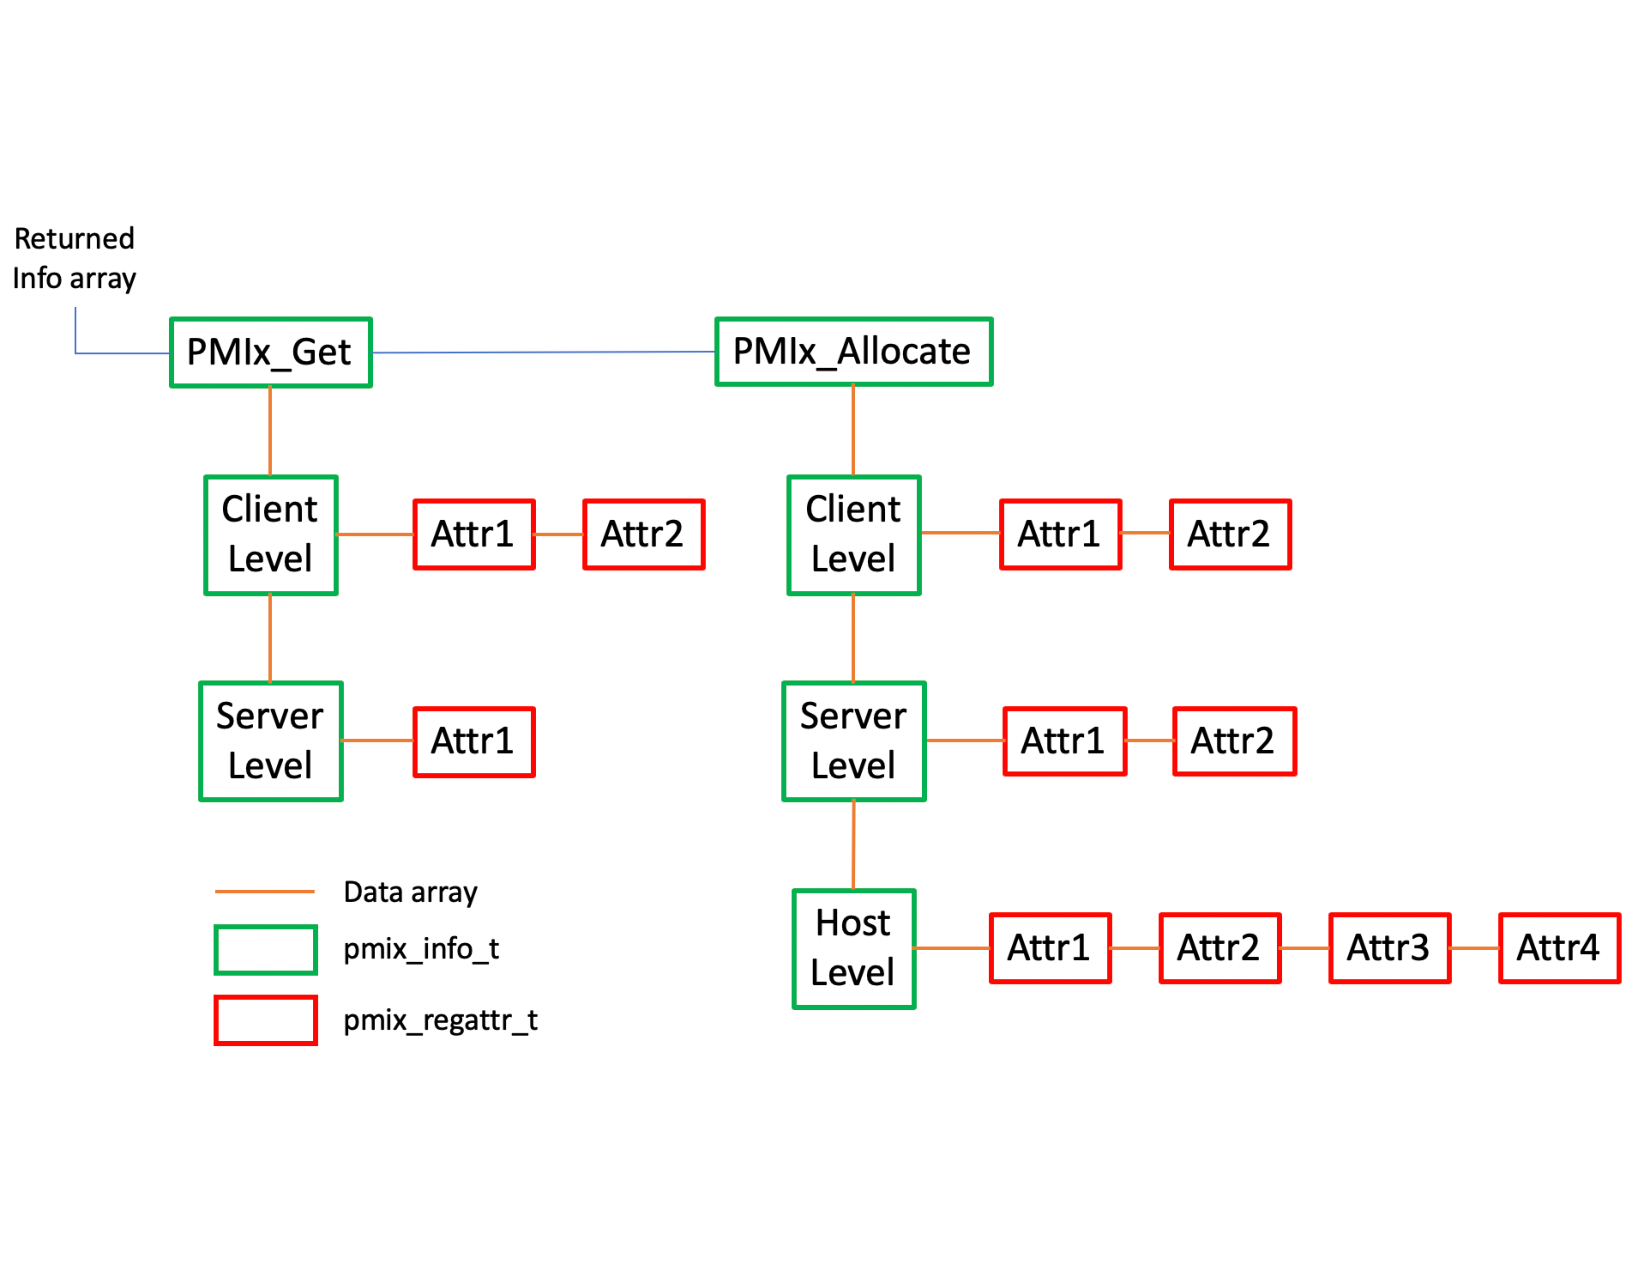
\includegraphics[clip,width=0.75\textwidth]{figs/attrquery.pdf}
  \end{center}
  \caption{Returned information hierarchy for attribute support request}
  \label{fig:attrquery}
\end{figure*}
\endgroup

The array of returned structures, and their child arrays, are subject to the return rules for the \refapi{PMIx_Query_info_nb} \ac{API}. For example, a request for supported attributes of the \refapi{PMIx_Get} function that includes the \refarg{host} level will return values for the \refarg{client} and \refarg{server} levels, plus an array element with a \refarg{key} of \refattr{PMIX_HOST_ATTRIBUTES} and a value type of \refconst{PMIX_UNDEF} indicating that no attributes are supported at that level.

%%%%%%%%%%%%%%%%%%%%%%%%%%%%%%%%%%%%%%%%%%%%%%
%%%%%%%%%%%%%%%%%%%%%%%%%%%%%%%%%%%%%%%%%%%%%%
\section{Allocation Requests}
\label{chap:api_job_mgmt:alloc}

This section defines functionality to request new allocations from the \ac{RM}, and request modifications to existing allocations.
These are primarily used in the following scenarios:
\begin{itemize}
\item \textit{Evolving} applications that dynamically request and return resources as they execute
\item \textit{Malleable} environments where the scheduler redirects resources away from executing applications for higher priority jobs or load balancing
\item \textit{Resilient} applications that need to request replacement resources in the face of failures
\item \textit{Rigid} jobs where the user has requested a static allocation of resources for a fixed period of time, but realizes that they underestimated their required time while executing
\end{itemize}
\ac{PMIx} attempts to address this range of use-cases with a flexible \ac{API}.

%%%%%%%%%%%
\subsection{\code{PMIx_Allocation_request}}
\declareapi{PMIx_Allocation_request}

%%%%
\summary

Request an allocation operation from the host resource manager.

%%%%
\format

\versionMarker{3.0}
\cspecificstart
\begin{codepar}
pmix_status_t
PMIx_Allocation_request(pmix_alloc_directive_t directive,
                        pmix_info_t info[], size_t ninfo);
\end{codepar}
\cspecificend

\begin{arglist}
\argin{directive}{Allocation directive (handle)}
\argin{info}{Array of \refstruct{pmix_info_t} structures (array of handles)}
\argin{ninfo}{Number of elements in the \refarg{info} array (integer)}
\end{arglist}

Returns one of the following:

\begin{itemize}
    \item \refconst{PMIX_SUCCESS}, indicating that the request was processed and returned \textit{success}
    \item a PMIx error constant indicating either an error in the input or that the request was refused
\end{itemize}

\reqattrstart
\ac{PMIx} libraries are not required to directly support any attributes for this function. However, any provided attributes must be passed to the host \ac{SMS} daemon for processing, and the \ac{PMIx} library is \textit{required} to add the \refPRIAttributeItem{PMIX_USERID} and the \refPRIAttributeItem{PMIX_GRPID} attributes of the client process making the request.

\divider

Host environments that implement support for this operation are required to support the following attributes:

\pasteAttributeItem{PMIX_ALLOC_ID}
\pasteAttributeItem{PMIX_ALLOC_NUM_NODES}
\pasteAttributeItem{PMIX_ALLOC_NUM_CPUS}
\pasteAttributeItem{PMIX_ALLOC_TIME}

\reqattrend

\optattrstart
The following attributes are optional for host environments that support this operation:

\pasteAttributeItem{PMIX_ALLOC_NODE_LIST}
\pasteAttributeItem{PMIX_ALLOC_NUM_CPU_LIST}
\pasteAttributeItem{PMIX_ALLOC_CPU_LIST}
\pasteAttributeItem{PMIX_ALLOC_MEM_SIZE}
\pasteAttributeItem{PMIX_ALLOC_NETWORK}
\pasteAttributeItem{PMIX_ALLOC_NETWORK_ID}
\pasteAttributeItem{PMIX_ALLOC_BANDWIDTH}
\pasteAttributeItem{PMIX_ALLOC_NETWORK_QOS}
\pasteAttributeItem{PMIX_ALLOC_NETWORK_TYPE}
\pasteAttributeItem{PMIX_ALLOC_NETWORK_PLANE}
\pasteAttributeItem{PMIX_ALLOC_NETWORK_ENDPTS}
\pasteAttributeItem{PMIX_ALLOC_NETWORK_ENDPTS_NODE}
\pasteAttributeItem{PMIX_ALLOC_NETWORK_SEC_KEY}

\optattrend

%%%%
\descr

Request an allocation operation from the host resource manager.
Several broad categories are envisioned, including the ability to:

\begin{compactitem}
%
\item Request allocation of additional resources, including memory, bandwidth, and compute.
This should be accomplished in a non-blocking manner so that the application can continue to progress while waiting for resources to become available.
Note that the new allocation will be disjoint from (i.e., not affiliated with) the allocation of the requestor - thus the termination of one allocation will not impact the other.
%
\item Extend the reservation on currently allocated resources, subject to scheduling availability and priorities.
This includes extending the time limit on current resources, and/or requesting additional resources be allocated to the requesting job.
Any additional allocated resources will be considered as part of the current allocation, and thus will be released at the same time.
%
\item Return no-longer-required resources to the scheduler.
This includes the ``loan'' of resources back to the scheduler with a promise to return them upon subsequent request.
\end{compactitem}

%%%%%%%%%%%
\subsection{\code{PMIx_Allocation_request_nb}}
\declareapi{PMIx_Allocation_request_nb}

%%%%
\summary

Request an allocation operation from the host resource manager.

%%%%
\format

\versionMarker{2.0}
\cspecificstart
\begin{codepar}
pmix_status_t
PMIx_Allocation_request_nb(pmix_alloc_directive_t directive,
                           pmix_info_t info[], size_t ninfo,
                           pmix_info_cbfunc_t cbfunc, void *cbdata);
\end{codepar}
\cspecificend

\begin{arglist}
\argin{directive}{Allocation directive (handle)}
\argin{info}{Array of \refstruct{pmix_info_t} structures (array of handles)}
\argin{ninfo}{Number of elements in the \refarg{info} array (integer)}
\argin{cbfunc}{Callback function \refapi{pmix_info_cbfunc_t} (function reference)}
\argin{cbdata}{Data to be passed to the callback function (memory reference)}
\end{arglist}

Returns one of the following:

\begin{itemize}
    \item \refconst{PMIX_SUCCESS}, indicating that the request is being processed by the host environment - result will be returned in the provided \refarg{cbfunc}. Note that the library must not invoke the callback function prior to returning from the \ac{API}.
    \item \refconst{PMIX_OPERATION_SUCCEEDED}, indicating that the request was immediately processed and returned \textit{success} - the \refarg{cbfunc} will \textit{not} be called
    \item a PMIx error constant indicating either an error in the input or that the request was immediately processed and failed - the \refarg{cbfunc} will \textit{not} be called
\end{itemize}

\reqattrstart
\ac{PMIx} libraries are not required to directly support any attributes for this function. However, any provided attributes must be passed to the host \ac{SMS} daemon for processing, and the \ac{PMIx} library is \textit{required} to add the \refPRIAttributeItem{PMIX_USERID} and the \refPRIAttributeItem{PMIX_GRPID} attributes of the client process making the request.

\divider

Host environments that implement support for this operation are required to support the following attributes:

\pasteAttributeItem{PMIX_ALLOC_ID}
\pasteAttributeItem{PMIX_ALLOC_NUM_NODES}
\pasteAttributeItem{PMIX_ALLOC_NUM_CPUS}
\pasteAttributeItem{PMIX_ALLOC_TIME}

\reqattrend

\optattrstart
The following attributes are optional for host environments that support this operation:

\pasteAttributeItem{PMIX_ALLOC_NODE_LIST}
\pasteAttributeItem{PMIX_ALLOC_NUM_CPU_LIST}
\pasteAttributeItem{PMIX_ALLOC_CPU_LIST}
\pasteAttributeItem{PMIX_ALLOC_MEM_SIZE}
\pasteAttributeItem{PMIX_ALLOC_NETWORK}
\pasteAttributeItem{PMIX_ALLOC_NETWORK_ID}
\pasteAttributeItem{PMIX_ALLOC_BANDWIDTH}
\pasteAttributeItem{PMIX_ALLOC_NETWORK_QOS}
\pasteAttributeItem{PMIX_ALLOC_NETWORK_TYPE}
\pasteAttributeItem{PMIX_ALLOC_NETWORK_PLANE}
\pasteAttributeItem{PMIX_ALLOC_NETWORK_ENDPTS}
\pasteAttributeItem{PMIX_ALLOC_NETWORK_ENDPTS_NODE}
\pasteAttributeItem{PMIX_ALLOC_NETWORK_SEC_KEY}

\optattrend

%%%%
\descr

Non-blocking form of the \refapi{PMIx_Allocation_request} \ac{API}.


%%%%%%%%%%%%%%%%%%%%%%%%%%%%%%%%%%%%%%%%%%%%%%
%%%%%%%%%%%%%%%%%%%%%%%%%%%%%%%%%%%%%%%%%%%%%%
\section{Job Control}
\label{chap:api_job_mgmt:jctrl}

This section defines \acp{API} that enable the application and host environment to coordinate the response to failures and other events.
This can include requesting termination of the entire job or a subset of processes within a job, but can
also be used in combination with other \ac{PMIx} capabilities (e.g., allocation support and event notification) for more nuanced responses. For example, an application notified of an incipient over-temperature condition on a node could use the \refapi{PMIx_Allocation_request_nb} interface to request replacement nodes while simultaneously using the \refapi{PMIx_Job_control_nb} interface to direct that a checkpoint event be delivered to all processes in the application. If replacement resources are not available, the application might use the \refapi{PMIx_Job_control_nb} interface to request that the job continue at a lower power setting, perhaps sufficient to avoid the over-temperature failure.

The job control \acp{API} can also be used by an application to register itself as available for preemption when operating in an environment such as a cloud or where incentives, financial or otherwise, are provided to jobs willing to be preempted. Registration can include attributes indicating how many resources are being offered for preemption (e.g., all or only some portion), whether the application will require time to prepare for preemption, etc. Jobs that
request a warning will receive an event notifying them of an impending preemption (possibly including information as to the resources that will be taken away, how much time the application will be given prior to being preempted, whether the preemption will be a suspension or full termination, etc.) so they have an opportunity to save
their work. Once the application is ready, it calls the provided event completion callback function to indicate that
the SMS is free to suspend or terminate it, and can include directives regarding any desired restart.

%%%%%%%%%%%
\subsection{\code{PMIx_Job_control}}
\declareapi{PMIx_Job_control}

%%%%
\summary

Request a job control action.

%%%%
\format

\versionMarker{3.0}
\cspecificstart
\begin{codepar}
pmix_status_t
PMIx_Job_control(const pmix_proc_t targets[], size_t ntargets,
                 const pmix_info_t directives[], size_t ndirs)
\end{codepar}
\cspecificend

\begin{arglist}
\argin{targets}{Array of proc structures (array of handles)}
\argin{ntargets}{Number of element in the \refarg{targets} array (integer)}
\argin{directives}{Array of info structures (array of handles)}
\argin{ndirs}{Number of element in the \refarg{directives} array (integer)}
\argin{cbfunc}{Callback function \refapi{pmix_info_cbfunc_t} (function reference)}
\argin{cbdata}{Data to be passed to the callback function (memory reference)}
\end{arglist}

Returns one of the following:

\begin{itemize}
    \item \refconst{PMIX_SUCCESS}, indicating that the request was processed by the host environment and returned \textit{success}
    \item a \ac{PMIx} error constant indicating either an error in the input or that the request was refused
\end{itemize}

\reqattrstart
\ac{PMIx} libraries are not required to directly support any attributes for this function. However, any provided attributes must be passed to the host \ac{SMS} daemon for processing, and the \ac{PMIx} library is \textit{required} to add the \refPRIAttributeItem{PMIX_USERID} and the \refPRIAttributeItem{PMIX_GRPID} attributes of the client process making the request.

\divider

Host environments that implement support for this operation are required to support the following attributes:

\pastePRRTEAttributeItem{PMIX_JOB_CTRL_ID}
\pastePRRTEAttributeItem{PMIX_JOB_CTRL_PAUSE}
\pastePRRTEAttributeItem{PMIX_JOB_CTRL_RESUME}
\pastePRRTEAttributeItem{PMIX_JOB_CTRL_KILL}
\pastePRRTEAttributeItem{PMIX_JOB_CTRL_SIGNAL}
\pastePRRTEAttributeItem{PMIX_JOB_CTRL_TERMINATE}
\pastePRRTEAttributeItem{PMIX_REGISTER_CLEANUP}
\pastePRRTEAttributeItem{PMIX_REGISTER_CLEANUP_DIR}
\pastePRRTEAttributeItem{PMIX_CLEANUP_RECURSIVE}
\pastePRRTEAttributeItem{PMIX_CLEANUP_EMPTY}
\pastePRRTEAttributeItem{PMIX_CLEANUP_IGNORE}
\pastePRRTEAttributeItem{PMIX_CLEANUP_LEAVE_TOPDIR}

\reqattrend

\optattrstart
The following attributes are optional for host environments that support this operation:

\pasteAttributeItem{PMIX_JOB_CTRL_CANCEL}
\pasteAttributeItem{PMIX_JOB_CTRL_RESTART}
\pasteAttributeItem{PMIX_JOB_CTRL_CHECKPOINT}
\pasteAttributeItem{PMIX_JOB_CTRL_CHECKPOINT_EVENT}
\pasteAttributeItem{PMIX_JOB_CTRL_CHECKPOINT_SIGNAL}
\pasteAttributeItem{PMIX_JOB_CTRL_CHECKPOINT_TIMEOUT}
\pasteAttributeItem{PMIX_JOB_CTRL_CHECKPOINT_METHOD}
\pasteAttributeItem{PMIX_JOB_CTRL_PROVISION}
\pasteAttributeItem{PMIX_JOB_CTRL_PROVISION_IMAGE}
\pasteAttributeItem{PMIX_JOB_CTRL_PREEMPTIBLE}

\optattrend

%%%%
\descr

Request a job control action.
The \refarg{targets} array identifies the processes to which the requested job control action is to be applied.
A \code{NULL} value can be used to indicate all processes in the caller's namespace.
The use of \refconst{PMIX_RANK_WILDARD} can also be used to indicate that all processes in the given namespace are to be included.

The directives are provided as \refstruct{pmix_info_t} structures in the \refarg{directives} array.
The callback function provides a \refarg{status} to indicate whether or not the request was granted, and to provide some information as to the reason for any denial in the \refapi{pmix_info_cbfunc_t} array of \refstruct{pmix_info_t} structures.

%%%%%%%%%%%
\subsection{\code{PMIx_Job_control_nb}}
\declareapi{PMIx_Job_control_nb}

%%%%
\summary

Request a job control action.

%%%%
\format

\versionMarker{2.0}
\cspecificstart
\begin{codepar}
pmix_status_t
PMIx_Job_control_nb(const pmix_proc_t targets[], size_t ntargets,
                    const pmix_info_t directives[], size_t ndirs,
                    pmix_info_cbfunc_t cbfunc, void *cbdata)
\end{codepar}
\cspecificend

\begin{arglist}
\argin{targets}{Array of proc structures (array of handles)}
\argin{ntargets}{Number of element in the \refarg{targets} array (integer)}
\argin{directives}{Array of info structures (array of handles)}
\argin{ndirs}{Number of element in the \refarg{directives} array (integer)}
\argin{cbfunc}{Callback function \refapi{pmix_info_cbfunc_t} (function reference)}
\argin{cbdata}{Data to be passed to the callback function (memory reference)}
\end{arglist}

Returns one of the following:

\begin{itemize}
    \item \refconst{PMIX_SUCCESS}, indicating that the request is being processed by the host environment - result will be returned in the provided \refarg{cbfunc}. Note that the library must not invoke the callback function prior to returning from the \ac{API}.
    \item \refconst{PMIX_OPERATION_SUCCEEDED}, indicating that the request was immediately processed and returned \textit{success} - the \refarg{cbfunc} will \textit{not} be called
    \item a PMIx error constant indicating either an error in the input or that the request was immediately processed and failed - the \refarg{cbfunc} will \textit{not} be called
\end{itemize}

\reqattrstart
\ac{PMIx} libraries are not required to directly support any attributes for this function. However, any provided attributes must be passed to the host \ac{SMS} daemon for processing, and the \ac{PMIx} library is \textit{required} to add the \refPRIAttributeItem{PMIX_USERID} and the \refPRIAttributeItem{PMIX_GRPID} attributes of the client process making the request.

\divider

Host environments that implement support for this operation are required to support the following attributes:

\pastePRRTEAttributeItem{PMIX_JOB_CTRL_ID}
\pastePRRTEAttributeItem{PMIX_JOB_CTRL_PAUSE}
\pastePRRTEAttributeItem{PMIX_JOB_CTRL_RESUME}
\pastePRRTEAttributeItem{PMIX_JOB_CTRL_KILL}
\pastePRRTEAttributeItem{PMIX_JOB_CTRL_SIGNAL}
\pastePRRTEAttributeItem{PMIX_JOB_CTRL_TERMINATE}
\pastePRRTEAttributeItem{PMIX_REGISTER_CLEANUP}
\pastePRRTEAttributeItem{PMIX_REGISTER_CLEANUP_DIR}
\pastePRRTEAttributeItem{PMIX_CLEANUP_RECURSIVE}
\pastePRRTEAttributeItem{PMIX_CLEANUP_EMPTY}
\pastePRRTEAttributeItem{PMIX_CLEANUP_IGNORE}
\pastePRRTEAttributeItem{PMIX_CLEANUP_LEAVE_TOPDIR}

\reqattrend

\optattrstart
The following attributes are optional for host environments that support this operation:

\pasteAttributeItem{PMIX_JOB_CTRL_CANCEL}
\pasteAttributeItem{PMIX_JOB_CTRL_RESTART}
\pasteAttributeItem{PMIX_JOB_CTRL_CHECKPOINT}
\pasteAttributeItem{PMIX_JOB_CTRL_CHECKPOINT_EVENT}
\pasteAttributeItem{PMIX_JOB_CTRL_CHECKPOINT_SIGNAL}
\pasteAttributeItem{PMIX_JOB_CTRL_CHECKPOINT_TIMEOUT}
\pasteAttributeItem{PMIX_JOB_CTRL_CHECKPOINT_METHOD}
\pasteAttributeItem{PMIX_JOB_CTRL_PROVISION}
\pasteAttributeItem{PMIX_JOB_CTRL_PROVISION_IMAGE}
\pasteAttributeItem{PMIX_JOB_CTRL_PREEMPTIBLE}

\optattrend

%%%%
\descr

Non-blocking form of the \refapi{PMIx_Job_control} \ac{API}.
The \refarg{targets} array identifies the processes to which the requested job control action is to be applied.
A \code{NULL} value can be used to indicate all processes in the caller's namespace.
The use of \refconst{PMIX_RANK_WILDARD} can also be used to indicate that all processes in the given namespace are to be included.

The directives are provided as \refstruct{pmix_info_t} structures in the \refarg{directives} array.
The callback function provides a \refarg{status} to indicate whether or not the request was granted, and to provide some information as to the reason for any denial in the \refapi{pmix_info_cbfunc_t} array of \refstruct{pmix_info_t} structures.



%%%%%%%%%%%%%%%%%%%%%%%%%%%%%%%%%%%%%%%%%%%%%%
%%%%%%%%%%%%%%%%%%%%%%%%%%%%%%%%%%%%%%%%%%%%%%
\section{Process and Job Monitoring}
\label{chap:api_job_mgmt:monitor}

In addition to external faults, a common problem encountered in \ac{HPC} applications is a failure to make
progress due to some internal conflict in the computation. These situations can
result in a significant waste of resources as the \ac{SMS} is unaware of the problem, and thus cannot terminate the
job. Various watchdog methods have been developed for detecting this situation, including requiring a periodic ``heartbeat''
from the application and monitoring a specified file for changes in size and/or modification time.

At the request of \ac{SMS} vendors and members, a monitoring support interface has been included in the PMIx v2 standard. The defined \ac{API} allows applications to request monitoring, directing what is to be monitored, the frequency of the associated check, whether or not the application is to be notified (via the event notification subsystem) of stall detection, and other characteristics of the operation. In addition, heartbeat and file monitoring methods have been included in the \ac{PRI} but are active only when requested.

%%%%%%%%%%%
\subsection{\code{PMIx_Process_monitor}}
\declareapi{PMIx_Process_monitor}

%%%%
\summary

Request that application processes be monitored.

%%%%
\format

\versionMarker{3.0}
\cspecificstart
\begin{codepar}
pmix_status_t
PMIx_Process_monitor(const pmix_info_t *monitor, pmix_status_t error,
                     const pmix_info_t directives[], size_t ndirs)
\end{codepar}
\cspecificend

\begin{arglist}
\argin{monitor}{info (handle)}
\argin{error}{status (integer)}
\argin{directives}{Array of info structures (array of handles)}
\argin{ndirs}{Number of elements in the \refarg{directives} array (integer)}
\end{arglist}

Returns one of the following:

\begin{itemize}
    \item \refconst{PMIX_SUCCESS}, indicating that the request was processed and returned \textit{success}
    \item a PMIx error constant indicating either an error in the input or that the request was refused
\end{itemize}

\optattrstart
The following attributes may be implemented by a \ac{PMIx} library or by the host environment. If supported by the \ac{PMIx} server library, then the library must not pass the supported attributes to the host environment. All attributes not directly supported by the server library must be passed to the host environment if it supports this operation, and the library is \textit{required} to add the \refPRIAttributeItem{PMIX_USERID} and the \refPRIAttributeItem{PMIX_GRPID} attributes of the requesting process:

\pastePRIAttributeItem{PMIX_MONITOR_ID}
\pastePRIAttributeItem{PMIX_MONITOR_CANCEL}
\pastePRIAttributeItem{PMIX_MONITOR_APP_CONTROL}
\pastePRIAttributeItem{PMIX_MONITOR_HEARTBEAT}
\pastePRIAttributeItem{PMIX_MONITOR_HEARTBEAT_TIME}
\pastePRIAttributeItem{PMIX_MONITOR_HEARTBEAT_DROPS}
\pastePRIAttributeItem{PMIX_MONITOR_FILE}
\pastePRIAttributeItem{PMIX_MONITOR_FILE_SIZE}
\pastePRIAttributeItem{PMIX_MONITOR_FILE_ACCESS}
\pastePRIAttributeItem{PMIX_MONITOR_FILE_MODIFY}
\pastePRIAttributeItem{PMIX_MONITOR_FILE_CHECK_TIME}
\pastePRIAttributeItem{PMIX_MONITOR_FILE_DROPS}

\optattrend

%%%%
\descr

Request that application processes be monitored via several possible methods.
For example, that the server monitor this process for periodic heartbeats as an indication that the process has not become ``wedged''.
When a monitor detects the specified alarm condition, it will generate an event notification using the provided error code and passing along any available relevant information.
It is up to the caller to register a corresponding event handler.

The \refarg{monitor} argument is an attribute indicating the type of monitor being requested.
For example, \refattr{PMIX_MONITOR_FILE} to indicate that the requestor is asking that a file be monitored.

The \refarg{error} argument is the status code to be used when generating an event notification alerting that the monitor has been triggered.
The range of the notification defaults to \refconst{PMIX_RANGE_NAMESPACE}.
This can be changed by providing a \refconst{PMIX_RANGE} directive.

The \refarg{directives} argument characterizes the monitoring request (e.g., monitor file size) and frequency of checking to be done


%%%%%%%%%%%
\subsection{\code{PMIx_Process_monitor_nb}}
\declareapi{PMIx_Process_monitor_nb}

%%%%
\summary

Request that application processes be monitored.

%%%%
\format

\versionMarker{2.0}
\cspecificstart
\begin{codepar}
pmix_status_t
PMIx_Process_monitor_nb(const pmix_info_t *monitor, pmix_status_t error,
                        const pmix_info_t directives[], size_t ndirs,
                        pmix_info_cbfunc_t cbfunc, void *cbdata)
\end{codepar}
\cspecificend

\begin{arglist}
\argin{monitor}{info (handle)}
\argin{error}{status (integer)}
\argin{directives}{Array of info structures (array of handles)}
\argin{ndirs}{Number of elements in the \refarg{directives} array (integer)}
\argin{cbfunc}{Callback function \refapi{pmix_info_cbfunc_t} (function reference)}
\argin{cbdata}{Data to be passed to the callback function (memory reference)}
\end{arglist}

Returns one of the following:

\begin{itemize}
    \item \refconst{PMIX_SUCCESS}, indicating that the request is being processed by the host environment - result will be returned in the provided \refarg{cbfunc}. Note that the library must not invoke the callback function prior to returning from the \ac{API}.
    \item \refconst{PMIX_OPERATION_SUCCEEDED}, indicating that the request was immediately processed and returned \textit{success} - the \refarg{cbfunc} will \textit{not} be called
    \item a PMIx error constant indicating either an error in the input or that the request was immediately processed and failed - the \refarg{cbfunc} will \textit{not} be called
\end{itemize}

\optattrstart
The following attributes may be implemented by a \ac{PMIx} library or by the host environment. If supported by the \ac{PMIx} server library, then the library must not pass the supported attributes to the host environment. All attributes not directly supported by the server library must be passed to the host environment if it supports this operation, and the library is \textit{required} to add the \refPRIAttributeItem{PMIX_USERID} and the \refPRIAttributeItem{PMIX_GRPID} attributes of the requesting process:

\pastePRIAttributeItem{PMIX_MONITOR_ID}
\pastePRIAttributeItem{PMIX_MONITOR_CANCEL}
\pastePRIAttributeItem{PMIX_MONITOR_APP_CONTROL}
\pastePRIAttributeItem{PMIX_MONITOR_HEARTBEAT}
\pastePRIAttributeItem{PMIX_MONITOR_HEARTBEAT_TIME}
\pastePRIAttributeItem{PMIX_MONITOR_HEARTBEAT_DROPS}
\pastePRIAttributeItem{PMIX_MONITOR_FILE}
\pastePRIAttributeItem{PMIX_MONITOR_FILE_SIZE}
\pastePRIAttributeItem{PMIX_MONITOR_FILE_ACCESS}
\pastePRIAttributeItem{PMIX_MONITOR_FILE_MODIFY}
\pastePRIAttributeItem{PMIX_MONITOR_FILE_CHECK_TIME}
\pastePRIAttributeItem{PMIX_MONITOR_FILE_DROPS}

\optattrend

%%%%
\descr


Non-blocking form of the \refapi{PMIx_Process_monitor} \ac{API}. The \refarg{cbfunc} function provides a \refarg{status} to indicate whether or not the request was granted, and to provide some information as to the reason for any denial in the \refapi{pmix_info_cbfunc_t} array of \refstruct{pmix_info_t} structures.

%%%%%%%%%%%
\subsection{\code{PMIx_Heartbeat}}
\declaremacro{PMIx_Heartbeat}

%%%%
\summary

Send a heartbeat to the \ac{PMIx} server library

%%%%
\format

\versionMarker{2.0}
\cspecificstart
\begin{codepar}
PMIx_Heartbeat(void)
\end{codepar}
\cspecificend


%%%%
\descr

A simplified macro wrapping \refapi{PMIx_Process_monitor_nb} that sends a heartbeat to the \ac{PMIx} server library.


%%%%%%%%%%%%%%%%%%%%%%%%%%%%%%%%%%%%%%%%%%%%%%
%%%%%%%%%%%%%%%%%%%%%%%%%%%%%%%%%%%%%%%%%%%%%%
\section{Logging}
\label{chap:api_job_mgmt:logging}

The logging interface supports posting information by applications and SMS elements to persistent storage. This function is \textit{not} intended for output of computational results, but rather for reporting status and saving state information such as inserting computation progress reports into the application's \ac{SMS} job log or error reports to the local syslog.

\subsection{\code{PMIx_Log}}
\declareapi{PMIx_Log}

%%%%
\summary

Log data to a data service.

%%%%
\format

\versionMarker{3.0}
\cspecificstart
\begin{codepar}
pmix_status_t
PMIx_Log(const pmix_info_t data[], size_t ndata,
         const pmix_info_t directives[], size_t ndirs)
\end{codepar}
\cspecificend

\begin{arglist}
\argin{data}{Array of info structures (array of handles)}
\argin{ndata}{Number of elements in the \refarg{data} array (\code{size_t})}
\argin{directives}{Array of info structures (array of handles)}
\argin{ndirs}{Number of elements in the \refarg{directives} array (\code{size_t})}
\end{arglist}

Return codes are one of the following:

\begin{constantdesc}
    \item \refconst{PMIX_SUCCESS} The logging request was successful.
    \item \refconst{PMIX_ERR_BAD_PARAM} The logging request contains at least one incorrect entry.
    \item \refconst{PMIX_ERR_NOT_SUPPORTED} The \ac{PMIx} implementation or host environment does not support this function.
\end{constantdesc}

\reqattrstart
If the \ac{PMIx} library does not itself perform this operation, then it is required to pass any attributes provided by the client to the host environment for processing. In addition, it must include the following attributes in the passed \refarg{info} array:

\pastePRIAttributeItem{PMIX_USERID}
\pastePRIAttributeItem{PMIX_GRPID}

\divider

Host environments or \ac{PMIx} libraries that implement support for this operation are required to support the following attributes:

\pastePRIAttributeItem{PMIX_LOG_STDERR}
\pastePRIAttributeItem{PMIX_LOG_STDOUT}
\pastePRIAttributeItem{PMIX_LOG_SYSLOG}
\pastePRIAttributeItem{PMIX_LOG_LOCAL_SYSLOG}
\pastePRIAttributeItem{PMIX_LOG_GLOBAL_SYSLOG}
\pastePRIAttributeItem{PMIX_LOG_SYSLOG_PRI}
\pastePRIAttributeItem{PMIX_LOG_ONCE}

\reqattrend

\optattrstart
The following attributes are optional for host environments or \ac{PMIx} libraries that support this operation:

\pastePRIAttributeItem{PMIX_LOG_SOURCE}
\pastePRIAttributeItem{PMIX_LOG_TIMESTAMP}
\pastePRIAttributeItem{PMIX_LOG_GENERATE_TIMESTAMP}
\pastePRIAttributeItem{PMIX_LOG_TAG_OUTPUT}
\pastePRIAttributeItem{PMIX_LOG_TIMESTAMP_OUTPUT}
\pastePRIAttributeItem{PMIX_LOG_XML_OUTPUT}
\pastePRRTEAttributeItem{PMIX_LOG_EMAIL}
\pastePRRTEAttributeItem{PMIX_LOG_EMAIL_ADDR}
\pastePRRTEAttributeItem{PMIX_LOG_EMAIL_SUBJECT}
\pastePRRTEAttributeItem{PMIX_LOG_EMAIL_MSG}
\pasteAttributeItem{PMIX_LOG_JOB_RECORD}
\pasteAttributeItem{PMIX_LOG_GLOBAL_DATASTORE}

\optattrend

%%%%
\descr

Log data subject to the services offered by the host environment. The data to be logged is provided in the \refarg{data} array. The (optional) \refarg{directives} can be used to direct the choice of logging channel.

\adviceuserstart
It is strongly recommended that the \refapi{PMIx_Log} API not be used by applications for streaming data as it is not a ``performant'' transport and can perturb the application since it involves the local \ac{PMIx} server and host \ac{SMS} daemon. Note that a return of \refconst{PMIX_SUCCESS} only denotes that the data was successfully handed to the appropriate system call (for local channels) or the host environment and does not indicate receipt at the final destination.
\adviceuserend

%
\subsection{\code{PMIx_Log_nb}}
\declareapi{PMIx_Log_nb}

%%%%
\summary

Log data to a data service.

%%%%
\format

\versionMarker{2.0}
\cspecificstart
\begin{codepar}
pmix_status_t
PMIx_Log_nb(const pmix_info_t data[], size_t ndata,
            const pmix_info_t directives[], size_t ndirs,
            pmix_op_cbfunc_t cbfunc, void *cbdata)
\end{codepar}
\cspecificend

\begin{arglist}
\argin{data}{Array of info structures (array of handles)}
\argin{ndata}{Number of elements in the \refarg{data} array (\code{size_t})}
\argin{directives}{Array of info structures (array of handles)}
\argin{ndirs}{Number of elements in the \refarg{directives} array (\code{size_t})}
\argin{cbfunc}{Callback function \refapi{pmix_op_cbfunc_t} (function reference)}
\argin{cbdata}{Data to be passed to the callback function (memory reference)}
\end{arglist}

Return codes are one of the following:

\begin{constantdesc}
\item \refconst{PMIX_SUCCESS} The logging request is valid and is being processed. The resulting status from the operation will be provided in the callback function. Note that the library must not invoke the callback function prior to returning from the \ac{API}.
\item \refconst{PMIX_OPERATION_SUCCEEDED}, indicating that the request was immediately processed and returned \textit{success} - the \refarg{cbfunc} will \textit{not} be called
\item \refconst{PMIX_ERR_BAD_PARAM} The logging request contains at least one incorrect entry that prevents it from being processed. The callback function will not be called.
\item \refconst{PMIX_ERR_NOT_SUPPORTED} The \ac{PMIx} implementation does not support this function. The callback function will not be called.
\end{constantdesc}

\reqattrstart
If the \ac{PMIx} library does not itself perform this operation, then it is required to pass any attributes provided by the client to the host environment for processing. In addition, it must include the following attributes in the passed \refarg{info} array:

\pastePRIAttributeItem{PMIX_USERID}
\pastePRIAttributeItem{PMIX_GRPID}

\divider

Host environments or \ac{PMIx} libraries that implement support for this operation are required to support the following attributes:

\pastePRIAttributeItem{PMIX_LOG_STDERR}
\pastePRIAttributeItem{PMIX_LOG_STDOUT}
\pastePRIAttributeItem{PMIX_LOG_SYSLOG}
\pastePRIAttributeItem{PMIX_LOG_LOCAL_SYSLOG}
\pastePRIAttributeItem{PMIX_LOG_GLOBAL_SYSLOG}
\pastePRIAttributeItem{PMIX_LOG_SYSLOG_PRI}
\pastePRIAttributeItem{PMIX_LOG_ONCE}

\reqattrend

\optattrstart
The following attributes are optional for host environments or \ac{PMIx} libraries that support this operation:

\pastePRIAttributeItem{PMIX_LOG_SOURCE}
\pastePRIAttributeItem{PMIX_LOG_TIMESTAMP}
\pastePRIAttributeItem{PMIX_LOG_GENERATE_TIMESTAMP}
\pastePRIAttributeItem{PMIX_LOG_TAG_OUTPUT}
\pastePRIAttributeItem{PMIX_LOG_TIMESTAMP_OUTPUT}
\pastePRIAttributeItem{PMIX_LOG_XML_OUTPUT}
\pastePRRTEAttributeItem{PMIX_LOG_EMAIL}
\pastePRRTEAttributeItem{PMIX_LOG_EMAIL_ADDR}
\pastePRRTEAttributeItem{PMIX_LOG_EMAIL_SUBJECT}
\pastePRRTEAttributeItem{PMIX_LOG_EMAIL_MSG}
\pasteAttributeItem{PMIX_LOG_JOB_RECORD}
\pasteAttributeItem{PMIX_LOG_GLOBAL_DATASTORE}

\optattrend

%%%%
\descr

Log data subject to the services offered by the host environment. The data to be logged is provided in the \refarg{data} array. The (optional) \refarg{directives} can be used to direct the choice of logging channel.
The callback function will be executed when the log operation has been completed. The \refarg{data} and \refarg{directives} arrays must be maintained until the callback is provided.

\adviceuserstart
It is strongly recommended that the \refapi{PMIx_Log_nb} API not be used by applications for streaming data as it is not a ``performant'' transport and can perturb the application since it involves the local \ac{PMIx} server and host \ac{SMS} daemon. Note that a return of \refconst{PMIX_SUCCESS} only denotes that the data was successfully handed to the appropriate system call (for local channels) or the host environment and does not indicate receipt at the final destination.
\adviceuserend

%%%%%%%%%%%%%%%%%%%%%%%%%%%%%%%%%%%%%%%%%%%%%%%%%


    % PMIx Process Sets and Groups
    %%%%%%%%%%%%%%%%%%%%%%%%%%%%%%%%%%%%%%%%%%%%%%%%%
% Chapter: Process Sets and Groups
%%%%%%%%%%%%%%%%%%%%%%%%%%%%%%%%%%%%%%%%%%%%%%%%%
\chapter{Process Sets and Groups}
\label{chap:api_sets_groups}

\ac{PMIx} supports two slightly related, but functionally different concepts
known as \emph{process sets} and \emph{process groups}. This chapter defines
these two concepts and describes how they are utilized, along with their
corresponding \acp{API}.

%%%%%%%%%%%%%%%%%%%%%%%%%%%%%%%%%%%%%%%%%%%%%%
%%%%%%%%%%%%%%%%%%%%%%%%%%%%%%%%%%%%%%%%%%%%%%
\section{Process Sets}
\label{chap:api_sets_groups:sets}

A \ac{PMIx} \emph{Process Set} is a user-provided or host environment assigned
label associated with a given set of application processes. Processes can
belong to multiple process \emph{sets} at a time. Definition of a \ac{PMIx}
process set typically occurs at time of application execution - e.g., on a
command line:

\cspecificstart
\begin{codepar}
\$ prun -n 4 --pset ocean myoceanapp : -n 3 --pset ice myiceapp
\end{codepar}
\cspecificend

In this example, the processes in the first application will be labeled with a \refattr{PMIX_PSET_NAMES} attribute of \emph{ocean} while those in the second application will be labeled with an \emph{ice} value. During the execution, application processes could lookup the process set attribute for any other process using \refapi{PMIx_Get}. Alternatively, other executing applications could utilize the \refapi{PMIx_Query_info_nb} \ac{API} to obtain the number of declared process sets in the system, a list of their names, and other information about them. In other words, the \emph{process set} identifier provides a label by which an application can derive information about a process and its application - it does \emph{not}, however, confer any operational function.

Host environments can create or delete process sets at any time, as well as
add and delete members from existing process sets, through the
\refapi{PMIx_server_define_process_set} and
\refapi{PMIx_server_delete_process_set} \acp{API}. \ac{PMIx} servers shall
notify all local clients of process set operations via the
\refconst{PMIX_PROCESS_SET_DEFINE} or \refconst{PMIX_PROCESS_SET_DELETE}
events.

\advicermstart
The host environment is responsible for ensuring:

\begin{itemize}
    \item consistent knowledge of process set membership across all involved
    \ac{PMIx} servers; and
    \item that process set names do not conflict with system-assigned namespaces within the scope of the set
\end{itemize}

\advicermend

Process \emph{sets} differ from process \emph{groups} in several key ways:

\begin{itemize}
    \item Process \emph{sets} have no implied relationship between their members - i.e., a process in a process set has no concept of a ``pset rank'' as it would in a process \emph{group}

    \item Process \emph{set} identifiers are set by the host environment -
    there are no \ac{PMIx} \acp{API} provided by which an application can
    change a process \emph{set} membership. In contrast, \ac{PMIx} process
    \emph{groups} can only be defined dynamically by the application.

    \item Process \emph{groups} can be used in calls to \ac{PMIx} operations. Members of process \emph{groups} that are involved in an operation are translated by their \ac{PMIx} server into their \emph{native} identifier prior to the operation being passed to the host environment. For example, an application can define a process group to consist of ranks 0 and 1 from the host-assigned namespace of \emph{210456}, identified by the group id of \emph{foo}. If the application subsequently calls the \refapi{PMIx_Fence} \ac{API} with a process identifier of \{foo, PMIX_RANK_WILDCARD\}, the \ac{PMIx} server will replace that identifier with an array consisting of \{210456, 0\} and \{210456, 1\} - the host-assigned identifiers of the participating processes - prior to passing the request up to the host environment

    \item Process \emph{groups} can request that the host environment assign a unique \code{size_t} \ac{PGCID} to the group at time of group construction. An \ac{MPI} library may, for example, use the \ac{PGCID} as the \ac{MPI} communicator identifier for the group.
\end{itemize}

The two concepts do, however, overlap in one specific area in that they both
involve collections of processes. Users desiring to create a process group
based on a process set could, for example, obtain the membership array of the
process set and use that as input to \refapi{PMIx_Group_construct}, perhaps
including the process set name as the group identifier for clarity. Note that
no linkage between the set and group of the same name is implied nor
maintained - e.g., changes in process set membership would not automatically be
reflected in the process group using the same identifier.


%%%%%%%%%%%
\subsection{Process Set Constants}

\versionMarker{4.0}
The \ac{PMIx} server is required to notify all local clients of changes to
process set membership, including the creation of new process sets as well as
their complete deletion. Client processes wishing to receive such
notifications must register for one or more of the following events:

\begin{constantdesc}
%
\declareconstitemNEW{PMIX_PROCESS_SET_DEFINE}
The host environment has defined a new process set, or has added members to
an existing process set.
%
\declareconstitemNEW{PMIX_PROCESS_SET_DELETE}
The host environment has removed members from an existing process set. If all
members of the set have been removed, then the set definition has been
deleted from the system.
%
\end{constantdesc}


%%%%%%%%%%%
\subsection{Process Set Attributes}

\versionMarker{4.0}
Several attributes are provided for querying the system regarding process sets.

%
\declareAttributeNEW{PMIX_QUERY_NUM_PSETS}{"pmix.qry.psetnum"}{size_t}{
Return the number of process sets defined in the specified range (defaults
to session).
}

%
\declareAttributeNEW{PMIX_QUERY_PSET_NAMES}{"pmix.qry.psets"}{pmix_data_array_t*}{
Return a \refstruct{pmix_data_array_t} containing an array of strings of the
process set names defined in the specified range (defaults to session).
}

%
\declareAttributeNEW{PMIX_QUERY_PSET_MEMBERSHIP}{"pmix.qry.pmems"}{pmix_proc_t*}{
Return a \refstruct{pmix_data_array_t} of \refstruct{pmix_proc_t} containing
the members of the specified process set.
}

In addition, a process can request (via \refapi{PMIx_Get}) the process sets to which a given process (including itself) belongs:

%
\declareAttributeNEW{PMIX_PSET_NAMES}{"pmix.pset.nm"}{pmix_data_array_t*}{
Returns an array of \code{char*} string names of the process sets in which the given process is a member.
}

%%%%%%%%%%%
\subsection{Process Set Constants}

\versionMarker{4.0}
The \ac{PMIx} server is required to notify all local clients of changes to
process set membership, including the creation of new process sets as well as
their complete deletion. Client processes wishing to receive such
notifications must register for one or more of the following events:

\begin{constantdesc}
%
\declareconstitemNEW{PMIX_PROCESS_SET_DEFINE}
The host environment has defined a new process set, or has added members to
an existing process set.
%
\declareconstitemNEW{PMIX_PROCESS_SET_DELETE}
The host environment has removed members from an existing process set. If all
members of the set have been removed, then the set definition has been
deleted from the system.
%
\end{constantdesc}



%%%%%%%%%%%%%%%%%%%%%%%%%%%%%%%%%%%%%%%%%%%%%%
%%%%%%%%%%%%%%%%%%%%%%%%%%%%%%%%%%%%%%%%%%%%%%
\section{Process Groups}
\label{chap:api_sets_groups:groups}

\ac{PMIx} \emph{Groups} are defined as a collection of processes desiring a common, unique identifier for operational purposes such as passing events or participating in \ac{PMIx} fence operations. As with processes that assemble via \refapi{PMIx_Connect}, each member of the group is provided with both the job-level information of any other namespace represented in the group, and the contact information for all group members. However, \emph{groups} differ from \refapi{PMIx_Connect} assemblages in the following key areas:

\begin{itemize}
    \item Relation to the host environment
    \begin{itemize}
        \item Calls to \refapi{PMIx_Connect} are relayed to the host environment. This means that the host \ac{RM} should treat the failure of any process in the specified assemblage as a reportable event and take appropriate action. However, the environment is not required to define a new identifier for the connected assemblage or any of its member processes, nor does it define a new rank for each process within that assemblage. In addition, the \ac{PMIx} server does not provide any tracking support for the assemblage. Thus, the caller is responsible for addressing members of the connected assemblage using their \ac{RM}-provided identifiers.

        \item Calls to \ac{PMIx} Group \acp{API} are first processed within the local \ac{PMIx} server. When constructed, the server creates a tracker that associates the specified processes with the user-provided group identifier, and assigns a new \emph{group rank} based on their relative position in the array of processes provided in the call to \refapi{PMIx_Group_construct}. Members of the group can subsequently utilize the group identifier in \ac{PMIx} function calls to address the group’s members, using either \refconst{PMIX_RANK_WILDCARD} to refer to all of them or the group-level rank of specific members. The \ac{PMIx} server will translate the specified processes into their \ac{RM}-assigned identifiers prior to passing the request up to its host. Thus, the host environment has no visibility into the group’s existence or membership.

\adviceuserstart
        User-provided group identifiers must be distinct from anything provided by the \ac{RM} so as to avoid collisions between group identifiers and \ac{RM}-assigned namespaces. This can usually be accomplished through the use of an application-specific prefix – e.g., ``myapp-foo''
\adviceuserend
    \end{itemize}
    \item Construction procedure
    \begin{itemize}
        \item \refapi{PMIx_Connect} calls require that every process call the \ac{API} before completing – i.e., it is modeled upon the bulk synchronous traditional \ac{MPI} connect/accept methodology. Thus, a given application thread can only be involved in one connect/accept operation at a time, and is blocked in that operation until all specified processes participate. In addition, there is no provision for replacing processes in the assemblage due to failure to participate, nor a mechanism by which a process might decline participation.

        \item \ac{PMIx} Groups are designed to be more flexible in their construction procedure by relaxing these constraints. While a standard blocking form of constructing groups is provided, the event notification system is utilized to provide a designated \emph{group leader} with the ability to replace participants that fail to participate within a given timeout period. This provides a mechanism by which the application can, if desired, replace members on-the-fly or allow the group to proceed with partial membership. In such cases, the final group membership is returned to all participants upon completion of the operation.

        Additionally, \ac{PMIx} supports dynamic definition of group membership based on an invite/join model. A process can asynchronously initiate construction of a group of any processes via the \refapi{PMIx_Group_invite} function call. Invitations are delivered via a \ac{PMIx} event (using the \refconst{PMIX_GROUP_INVITED} event) to the invited processes which can then either accept or decline the invitation using the \refapi{PMIx_Group_join} \ac{API}. The initiating process tracks responses by registering for the events generated by the call to \refapi{PMIx_Group_join}, timeouts, or process terminations, optionally replacing processes that decline the invitation, fail to respond in time, or terminate without responding. Upon completion of the operation, the final list of participants is communicated to each member of the new group.
    \end{itemize}
    \item Destruct procedure
    \begin{itemize}
        \item Processes that assemble via \refapi{PMIx_Connect} must all depart the assemblage together – i.e., no member can depart the assemblage while leaving the remaining members in it. Even the non-blocking form of \refapi{PMIx_Disconnect} retains this requirement in that members remain a part of the assemblage until all members have called \refapi{PMIx_Disconnect_nb}
        \item Members of a \ac{PMIx} Group may depart the group at any time via the \refapi{PMIx_Group_leave} \ac{API}. Other members are notified of the departure via the \refconst{PMIX_GROUP_LEFT} event to distinguish such events from those reporting process termination. This leaves the remaining members free to continue group operations. The \refapi{PMIx_Group_destruct} operation offers a collective method akin to \refapi{PMIx_Disconnect} for deconstructing the entire group.

        Note that applications supporting dynamic group behaviors such as asynchronous departure take responsibility for ensuring global consistency in the group definition prior to executing group collective operations - i.e., it is the application's responsibility to either ensure that knowledge of the current group membership is globally consistent across the participants, or to register for appropriate events to deal with the lack of consistency during the operation.
    \end{itemize}
\end{itemize}

In other words, members of \ac{PMIx} Groups are \emph{loosely coupled} as opposed to \emph{tightly connected} when constructed via \refapi{PMIx_Connect}. The relevant \acp{API} are explained below.

\adviceuserstart
The reliance on \ac{PMIx} events in the \ac{PMIx} Group concept dictates that processes utilizing these \acp{API} must register for the corresponding events. Failure to do so will likely lead to operational failures. Users are recommended to utilize the \refattr{PMIX_TIMEOUT} directive (or retain an internal timer) on calls to \ac{PMIx} Group \acp{API} (especially the blocking form of those functions) as processes that have not registered for required events will never respond.
\adviceuserend


%%%%%%%%%%%
\subsection{Group Operation Constants}
\declarestruct{pmix_group_operation_t}

\versionMarker{4.0}
The \refstruct{pmix_group_operation_t} structure is an enumerated type for specifying group operations. All values were originally defined in version 4 of the standard unless otherwise marked.

\begin{constantdesc}
%
\declareconstitemNEW{PMIX_GROUP_DECLINE}
Decline an invitation to join a \ac{PMIx} group - provided for readability of user code
%
\declareconstitemNEW{PMIX_GROUP_ACCEPT}
Accept an invitation to join a \ac{PMIx} group - provided for readability of user code
%
\declareconstitemNEW{PMIX_GROUP_CONSTRUCT}
Construct a group composed of the specified processes - used by a \ac{PMIx} server library to direct host operation
%
\declareconstitemNEW{PMIX_GROUP_DESTRUCT}
Destruct the specified group - used by a \ac{PMIx} server library to direct host operation
%
\end{constantdesc}


%%%%%%%%%%%
\subsection{Process Group Attributes}

\versionMarker{4.0}
Several attributes are provided for querying the system regarding process
groups.

%
\declareAttributeNEW{PMIX_QUERY_NUM_GROUPS}{"pmix.qry.pgrpnum"}{size_t}{
Return the number of process groups defined in the specified range (defaults
to session).
}

%
\declareAttributeNEW{PMIX_QUERY_GROUP_NAMES}{"pmix.qry.pgrp"}{pmix_data_array_t*}{
Return a \refstruct{pmix_data_array_t} containing an array of string names of
the process groups defined in the specified range (defaults to session).
}

%
\declareAttributeNEW{PMIX_QUERY_GROUP_MEMBERSHIP}{"pmix.qry.pgrpmems"}{pmix_data_array_t*}{
Return a \refstruct{pmix_data_array_t} of \refstruct{pmix_proc_t} containing
the members of the specified process group.
}

In addition, a process can request (via \refapi{PMIx_Get}) the process groups to which a given process (including itself) belongs:

%
\declareAttributeNEW{PMIX_GROUP_NAMES}{"pmix.pgrp.nm"}{pmix_data_array_t*}{
Returns an array of \code{char*} string names of the process groups in which the given process is a member.
}


%%%%%%%%%%%
\subsection{\code{PMIx_Group_construct}}
\declareapi{PMIx_Group_construct}

%%%%
\summary

Construct a \ac{PMIx} process group

%%%%
\format

\versionMarker{4.0}
\cspecificstart
\begin{codepar}
pmix_status_t
PMIx_Group_construct(const char grp[],
                     const pmix_proc_t procs[], size_t nprocs,
                     const pmix_info_t directives[], size_t ndirs,
                     pmix_info_t **results, size_t *nresults)
\end{codepar}
\cspecificend

\begin{arglist}
\argin{grp}{\code{NULL}-terminated character array of maximum size \refconst{PMIX_MAX_NSLEN} containing the group identifier (string)}
\argin{procs}{Array of \refstruct{pmix_proc_t} structures containing the \ac{PMIx} identifiers of the member processes (array of handles)}
\argin{nprocs}{Number of elements in the \refarg{procs} array (\code{size_t})}
\argin{directives}{Array of \refstruct{pmix_info_t} structures (array of handles)}
\argin{ndirs}{Number of elements in the \refarg{directives} array (\code{size_t})}
\arginout{results}{Pointer to a location where the array of \refstruct{pmix_info_t} describing the results of the operation is to be returned (pointer to handle)}
\arginout{nresults}{Pointer to a \code{size_t} location where the number of elements in \refarg{results} is to be returned (memory reference)}
\end{arglist}

Returns one of the following:

\begin{itemize}
    \item \refconst{PMIX_SUCCESS}, indicating that the request has been successfully completed
    \item \refconst{PMIX_ERR_NOT_SUPPORTED} The \ac{PMIx} library and/or the host \ac{RM} does not support this operation
    \item a \ac{PMIx} error constant indicating either an error in the input or that the request failed to be completed
\end{itemize}

\reqattrstart
The following attributes are \textit{required} to be supported by all \ac{PMIx} libraries that support this operation:

\pasteAttributeItem{PMIX_GROUP_LEADER}
\pasteAttributeItem{PMIX_GROUP_OPTIONAL}
\pasteAttributeItem{PMIX_GROUP_LOCAL_ONLY}

Host environments that support this operation are \textit{required} to provide the following attributes:

\pasteAttributeItem{PMIX_GROUP_ASSIGN_CONTEXT_ID}
\pasteAttributeItem{PMIX_GROUP_NOTIFY_TERMINATION}

\reqattrend

\optattrstart
The following attributes are optional for host environments that support this operation:

\pasteAttributeItem{PMIX_TIMEOUT}

\optattrend

\adviceimplstart
We recommend that implementation of the \refattr{PMIX_TIMEOUT} attribute be left to the host environment due to race condition considerations between completion of the operation versus internal timeout in the \ac{PMIx} server library. Implementers that choose to support \refattr{PMIX_TIMEOUT} directly in the \ac{PMIx} server library must take care to resolve the race condition and should avoid passing \refattr{PMIX_TIMEOUT} to the host environment so that multiple competing timeouts are not created.
\adviceimplend


%%%%
\descr

Construct a new group composed of the specified processes and identified with the provided group identifier. The group identifier is a user-defined, \code{NULL}-terminated character array of length less than or equal to \refconst{PMIX_MAX_NSLEN}. Only characters accepted by standard string comparison functions (e.g., \emph{strncmp}) are supported. Processes may engage in multiple simultaneous group construct operations so long as each is provided with a unique group ID. The \refarg{directives} array can be used to pass user-level directives regarding timeout constraints and other options available from the \ac{PMIx} server.

If the \refattr{PMIX_GROUP_NOTIFY_TERMINATION} attribute is provided and has a value of \code{true}, then either the construct leader (if \refattr{PMIX_GROUP_LEADER} is provided) or all participants who register for the \refconst{PMIX_GROUP_MEMBER_FAILED} event will receive events whenever a process fails or terminates prior to calling \refapi{PMIx_Group_construct} – i.e. if a \emph{group leader} is declared, \textit{only} that process will receive the event. In the absence of a declared leader, \textit{all} specified group members will receive the event.

The event will contain the identifier of the process that failed to join plus any other information that the host \ac{RM} provided. This provides an opportunity for the leader or the collective members to react to the event – e.g., to decide to proceed with a smaller group or to abort the operation. The decision is communicated to the \ac{PMIx} library in the results array at the end of the event handler. This allows \ac{PMIx} to properly adjust accounting for procedure completion. When construct is complete, the participating \ac{PMIx} servers will be alerted to any change in participants and each group member will receive an updated group membership (marked with the \refattr{PMIX_GROUP_MEMBERSHIP} attribute) as part of the \refarg{results} array returned by this \ac{API}.

Failure of the declared leader at any time will cause a \refconst{PMIX_GROUP_LEADER_FAILED} event to be delivered to all participants so they can optionally declare a new leader. A new leader is identified by providing the \refattr{PMIX_GROUP_LEADER} attribute in the results array in the return of the event handler. Only one process is allowed to return that attribute, thereby declaring itself as the new leader. Results of the leader selection will be communicated to all participants via a \refconst{PMIX_GROUP_LEADER_SELECTED} event identifying the new leader. If no leader was selected, then the \refstruct{pmix_info_t} provided to that event handler will include that information so the participants can take appropriate action.

Any participant that returns \refconst{PMIX_GROUP_CONSTRUCT_ABORT} from either the \refconst{PMIX_GROUP_MEMBER_FAILED} or the \refconst{PMIX_GROUP_LEADER_FAILED} event handler will cause the construct process to abort, returning from the call with a \refconst{PMIX_GROUP_CONSTRUCT_ABORT} status.

If the \refattr{PMIX_GROUP_NOTIFY_TERMINATION} attribute is not provided or has a value of \code{false}, then the \refapi{PMIx_Group_construct} operation will simply return an error whenever a proposed group member fails or terminates prior to calling \refapi{PMIx_Group_construct}.

Providing the \refattr{PMIX_GROUP_OPTIONAL} attribute with a value of \code{true} directs the \ac{PMIx} library to consider participation by any specified group member as non-required - thus, the operation will return \refconst{PMIX_SUCCESS} if all members participate, or \refconst{PMIX_ERR_PARTIAL_SUCCESS} if some members fail to participate. The \refarg{results} array will contain the final group membership in the latter case. Note that this use-case can cause the operation to hang if the \refattr{PMIX_TIMEOUT} attribute is not specified and one or more group members fail to call \refapi{PMIx_Group_construct} while continuing to execute. Also, note that no leader or member failed events will be generated during the operation.

Processes in a group under construction are not allowed to leave the group until group construction is complete. Upon completion of the construct procedure, each group member will have access to the job-level information of all namespaces represented in the group plus any information posted via \refapi{PMIx_Put} (subject to the usual scoping directives) for every group member.

\adviceimplstart
At the conclusion of the construct operation, the \ac{PMIx} library is \emph{required} to ensure that job-related information from each participating namespace plus any information posted by group members via \refapi{PMIx_Put} (subject to scoping directives) is available to each member via calls to \refapi{PMIx_Get}.
\adviceimplend

\advicermstart
The collective nature of this \ac{API} generally results in use of a fence-like operation by the backend host environment. Host environments that utilize the array of process participants as a \emph{signature} for such operations may experience potential conflicts should both a \refapi{PMIx_Group_construct} and a \refapi{PMIx_Fence} operation involving the same participants be simultaneously executed. As \ac{PMIx} allows for such use-cases, it is therefore the responsibility of the host environment to resolve any potential conflicts.
\advicermend

%%%%%%%%%%%
\subsection{\code{PMIx_Group_construct_nb}}
\declareapi{PMIx_Group_construct_nb}

%%%%
\summary

Non-blocking form of \refapi{PMIx_Group_construct}

%%%%
\format

\versionMarker{4.0}
\cspecificstart
\begin{codepar}
pmix_status_t
PMIx_Group_construct_nb(const char grp[],
                        const pmix_proc_t procs[], size_t nprocs,
                        const pmix_info_t directives[], size_t ndirs,
                        pmix_info_cbfunc_t cbfunc, void *cbdata)
\end{codepar}
\cspecificend

\begin{arglist}
\argin{grp}{\code{NULL}-terminated character array of maximum size \refconst{PMIX_MAX_NSLEN} containing the group identifier (string)}
\argin{procs}{Array of \refstruct{pmix_proc_t} structures containing the \ac{PMIx} identifiers of the member processes (array of handles)}
\argin{nprocs}{Number of elements in the \refarg{procs} array (\code{size_t})}
\argin{directives}{Array of \refstruct{pmix_info_t} structures (array of handles)}
\argin{ndirs}{Number of elements in the \refarg{directives} array (\code{size_t})}
\argin{cbfunc}{Callback function \refapi{pmix_info_cbfunc_t} (function reference)}
\argin{cbdata}{Data to be passed to the callback function (memory reference)}
\end{arglist}

Returns one of the following:

\begin{itemize}
\item \refconst{PMIX_SUCCESS} indicating that the request has been accepted for processing and the provided callback function will be executed upon completion of the operation. Note that the library \emph{must not} invoke the callback function prior to returning from the \ac{API}.
\item \refconst{PMIX_OPERATION_SUCCEEDED}, indicating that the request was immediately processed and returned \textit{success} - the \refarg{cbfunc} will \textit{not} be called
\item \refconst{PMIX_ERR_NOT_SUPPORTED} The \ac{PMIx} library does not support this operation - the \refarg{cbfunc} will \textit{not} be called
\item a non-zero \ac{PMIx} error constant indicating a reason for the request to have been rejected - the \refarg{cbfunc} will \textit{not} be called
\end{itemize}

If executed, the status returned in the provided callback function will be one of the following constants:

\begin{itemize}
\item \refconst{PMIX_SUCCESS} The operation succeeded and all specified members participated.
\item \refconst{PMIX_ERR_PARTIAL_SUCCESS} The operation succeeded but not all specified members participated - the final group membership is included in the callback function
\item \refconst{PMIX_ERR_NOT_SUPPORTED} While the \ac{PMIx} server supports this operation, the host \ac{RM} does not.
\item a non-zero \ac{PMIx} error constant indicating a reason for the request's failure
\end{itemize}

\reqattrstart
\ac{PMIx} libraries that choose not to support this operation \textit{must} return \refconst{PMIX_ERR_NOT_SUPPORTED} when the function is called.

The following attributes are \textit{required} to be supported by all \ac{PMIx} libraries that support this operation:

\pasteAttributeItem{PMIX_GROUP_LEADER}
\pasteAttributeItem{PMIX_GROUP_OPTIONAL}
\pasteAttributeItem{PMIX_GROUP_LOCAL_ONLY}

Host environments that support this operation are \textit{required} to provide the following attributes:

\pasteAttributeItem{PMIX_GROUP_ASSIGN_CONTEXT_ID}
\pasteAttributeItem{PMIX_GROUP_NOTIFY_TERMINATION}

\reqattrend

\optattrstart
The following attributes are optional for host environments that support this operation:

\pasteAttributeItem{PMIX_TIMEOUT}

\optattrend

\adviceimplstart
We recommend that implementation of the \refattr{PMIX_TIMEOUT} attribute be left to the host environment due to race condition considerations between completion of the operation versus internal timeout in the \ac{PMIx} server library. Implementers that choose to support \refattr{PMIX_TIMEOUT} directly in the \ac{PMIx} server library must take care to resolve the race condition and should avoid passing \refattr{PMIX_TIMEOUT} to the host environment so that multiple competing timeouts are not created.
\adviceimplend


%%%%
\descr

Non-blocking version of the \refapi{PMIx_Group_construct} operation. The callback function will be called once all group members have called either \refapi{PMIx_Group_construct} or \refapi{PMIx_Group_construct_nb}.

%%%%%%%%%%%
\subsection{\code{PMIx_Group_destruct}}
\declareapi{PMIx_Group_destruct}

%%%%
\summary

Destruct a \ac{PMIx} process group

%%%%
\format

\versionMarker{4.0}
\cspecificstart
\begin{codepar}
pmix_status_t
PMIx_Group_destruct(const char grp[],
                    const pmix_info_t directives[], size_t ndirs)
\end{codepar}
\cspecificend

\begin{arglist}
\argin{grp}{\code{NULL}-terminated character array of maximum size \refconst{PMIX_MAX_NSLEN} containing the identifier of the group to be destructed (string)}
\argin{directives}{Array of \refstruct{pmix_info_t} structures (array of handles)}
\argin{ndirs}{Number of elements in the \refarg{directives} array (\code{size_t})}
\end{arglist}

Returns one of the following:

\begin{itemize}
    \item \refconst{PMIX_SUCCESS}, indicating that the request has been successfully completed
    \item \refconst{PMIX_ERR_NOT_SUPPORTED} The \ac{PMIx} library and/or the host \ac{RM} does not support this operation
    \item a \ac{PMIx} error constant indicating either an error in the input or that the request failed to be completed
\end{itemize}

\reqattrstart
For implementations and host environments that support the operation, there are no identified required
attributes for this \ac{API}.
\reqattrend

\optattrstart
The following attributes are optional for host environments that support this operation:

\pasteAttributeItem{PMIX_TIMEOUT}

\optattrend

\adviceimplstart
We recommend that implementation of the \refattr{PMIX_TIMEOUT} attribute be left to the host environment due to race condition considerations between completion of the operation versus internal timeout in the \ac{PMIx} server library. Implementers that choose to support \refattr{PMIX_TIMEOUT} directly in the \ac{PMIx} server library must take care to resolve the race condition and should avoid passing \refattr{PMIX_TIMEOUT} to the host environment so that multiple competing timeouts are not created.
\adviceimplend


%%%%
\descr

Destruct a group identified by the provided group identifier. Processes may engage in multiple simultaneous group destruct operations so long as each involves a unique group ID. The \refarg{directives} array can be used to pass user-level directives regarding timeout constraints and other options available from the \ac{PMIx} server.

The destruct \ac{API} will return an error if any group process fails or terminates prior to calling \refapi{PMIx_Group_destruct} or its non-blocking version unless the \refattr{PMIX_GROUP_NOTIFY_TERMINATION} attribute was provided (with a value of \code{false}) at time of group construction. If notification was requested, then the \refconst{PMIX_GROUP_MEMBER_FAILED} event will be delivered for each process that fails to call destruct and the destruct tracker updated to account for the lack of participation. The \refapi{PMIx_Group_destruct} operation will subsequently return \refconst{PMIX_SUCCESS} when the remaining processes have all called destruct – i.e., the event will serve in place of return of an error.

\advicermstart
The collective nature of this \ac{API} generally results in use of a fence-like operation by the backend host environment. Host environments that utilize the array of process participants as a \emph{signature} for such operations may experience potential conflicts should both a \refapi{PMIx_Group_destruct} and a \refapi{PMIx_Fence} operation involving the same participants be simultaneously executed. As \ac{PMIx} allows for such use-cases, it is therefore the responsibility of the host environment to resolve any potential conflicts.
\advicermend

%%%%%%%%%%%
\subsection{\code{PMIx_Group_destruct_nb}}
\declareapi{PMIx_Group_destruct_nb}

%%%%
\summary

Non-blocking form of \refapi{PMIx_Group_destruct}

%%%%
\format

\versionMarker{4.0}
\cspecificstart
\begin{codepar}
pmix_status_t
PMIx_Group_destruct_nb(const char grp[],
                       const pmix_info_t directives[], size_t ndirs,
                       pmix_op_cbfunc_t cbfunc, void *cbdata)
\end{codepar}
\cspecificend

\begin{arglist}
\argin{grp}{\code{NULL}-terminated character array of maximum size \refconst{PMIX_MAX_NSLEN} containing the identifier of the group to be destructed (string)}
\argin{directives}{Array of \refstruct{pmix_info_t} structures (array of handles)}
\argin{ndirs}{Number of elements in the \refarg{directives} array (\code{size_t})}
\argin{cbfunc}{Callback function \refapi{pmix_op_cbfunc_t} (function reference)}
\argin{cbdata}{Data to be passed to the callback function (memory reference)}
\end{arglist}

Returns one of the following:

\begin{itemize}
    \item \refconst{PMIX_SUCCESS}, indicating that the request is being processed - result will be returned in the provided \refarg{cbfunc}. Note that the library \emph{must not} invoke the callback function prior to returning from the \ac{API}.
    \item \refconst{PMIX_OPERATION_SUCCEEDED}, indicating that the request was immediately processed and returned \textit{success} - the \refarg{cbfunc} will \textit{not} be called
    \item \refconst{PMIX_ERR_NOT_SUPPORTED} The \ac{PMIx} library does not support this operation - the \refarg{cbfunc} will \textit{not} be called
    \item a \ac{PMIx} error constant indicating either an error in the input or that the request was immediately processed and failed - the \refarg{cbfunc} will \textit{not} be called
\end{itemize}

If executed, the status returned in the provided callback function will be one of the following constants:

\begin{itemize}
\item \refconst{PMIX_SUCCESS} The operation was successfully completed
\item \refconst{PMIX_ERR_NOT_SUPPORTED} While the \ac{PMIx} server supports this operation, the host \ac{RM} does not.
\item a non-zero \ac{PMIx} error constant indicating a reason for the request's failure
\end{itemize}

\reqattrstart
\ac{PMIx} libraries that choose not to support this operation \textit{must} return \refconst{PMIX_ERR_NOT_SUPPORTED} when the function is called. For implementations and host environments that support the operation, there are no identified required
attributes for this \ac{API}.
\reqattrend

\optattrstart
The following attributes are optional for host environments that support this operation:

\pasteAttributeItem{PMIX_TIMEOUT}

\optattrend

\adviceimplstart
We recommend that implementation of the \refattr{PMIX_TIMEOUT} attribute be left to the host environment due to race condition considerations between completion of the operation versus internal timeout in the \ac{PMIx} server library. Implementers that choose to support \refattr{PMIX_TIMEOUT} directly in the \ac{PMIx} server library must take care to resolve the race condition and should avoid passing \refattr{PMIX_TIMEOUT} to the host environment so that multiple competing timeouts are not created.
\adviceimplend


%%%%
\descr

Non-blocking version of the \refapi{PMIx_Group_destruct} operation. The callback function will be called once all members of the group have executed either \refapi{PMIx_Group_destruct} or \refapi{PMIx_Group_destruct_nb}.

%%%%%%%%%%%
\subsection{\code{PMIx_Group_invite}}
\declareapi{PMIx_Group_invite}

%%%%
\summary

Asynchronously construct a \ac{PMIx} process group

%%%%
\format

\versionMarker{4.0}
\cspecificstart
\begin{codepar}
pmix_status_t
PMIx_Group_invite(const char grp[],
                  const pmix_proc_t procs[], size_t nprocs,
                  const pmix_info_t directives[], size_t ndirs,
                  pmix_info_t **results, size_t *nresult)
\end{codepar}
\cspecificend

\begin{arglist}
\argin{grp}{\code{NULL}-terminated character array of maximum size \refconst{PMIX_MAX_NSLEN} containing the group identifier (string)}
\argin{procs}{Array of \refstruct{pmix_proc_t} structures containing the \ac{PMIx} identifiers of the processes to be invited (array of handles)}
\argin{nprocs}{Number of elements in the \refarg{procs} array (\code{size_t})}
\argin{directives}{Array of \refstruct{pmix_info_t} structures (array of handles)}
\argin{ndirs}{Number of elements in the \refarg{directives} array (\code{size_t})}
\arginout{results}{Pointer to a location where the array of \refstruct{pmix_info_t} describing the results of the operation is to be returned (pointer to handle)}
\arginout{nresults}{Pointer to a \code{size_t} location where the number of elements in \refarg{results} is to be returned (memory reference)}
\end{arglist}

Returns one of the following:

\begin{itemize}
    \item \refconst{PMIX_SUCCESS}, indicating that the request has been successfully completed
    \item \refconst{PMIX_ERR_NOT_SUPPORTED} The \ac{PMIx} library and/or the host \ac{RM} does not support this operation
    \item a \ac{PMIx} error constant indicating either an error in the input or that the request failed to be completed
\end{itemize}

\reqattrstart
The following attributes are \textit{required} to be supported by all \ac{PMIx} libraries that support this operation:

\pasteAttributeItem{PMIX_GROUP_OPTIONAL}

Host environments that support this operation are \textit{required} to provide the following attributes:

\pasteAttributeItem{PMIX_GROUP_ASSIGN_CONTEXT_ID}
\pasteAttributeItem{PMIX_GROUP_NOTIFY_TERMINATION}
\reqattrend

\optattrstart
The following attributes are optional for host environments that support this operation:

\pasteAttributeItem{PMIX_TIMEOUT}

\optattrend

\adviceimplstart
We recommend that implementation of the \refattr{PMIX_TIMEOUT} attribute be left to the host environment due to race condition considerations between completion of the operation versus internal timeout in the \ac{PMIx} server library. Implementers that choose to support \refattr{PMIX_TIMEOUT} directly in the \ac{PMIx} server library must take care to resolve the race condition and should avoid passing \refattr{PMIX_TIMEOUT} to the host environment so that multiple competing timeouts are not created.
\adviceimplend


%%%%
\descr

Explicitly invite the specified processes to join a group. The process making the \refapi{PMIx_Group_invite} call is automatically declared to be the \emph{group leader}. Each invited process will be notified of the invitation via the \refconst{PMIX_GROUP_INVITED} event - the processes being invited must therefore register for the \refconst{PMIX_GROUP_INVITED} event in order to be notified of the invitation. Note that the \ac{PMIx} event notification system caches events - thus, no ordering of invite versus event registration is required.

The invitation event will include the identity of the inviting process plus the name of the group. When ready to respond, each invited process provides a response using either the blocking or non-blocking form of \refapi{PMIx_Group_join}. This will notify the inviting process that the invitation was either accepted (via the \refconst{PMIX_GROUP_INVITE_ACCEPTED} event) or declined (via the \refconst{PMIX_GROUP_INVITE_DECLINED} event). The \refconst{PMIX_GROUP_INVITE_ACCEPTED} event is captured by the \ac{PMIx} client library of the inviting process – i.e., the application itself does not need to register for this event. The library will track the number of accepting processes and alert the inviting process (by returning from the blocking form of \refapi{PMIx_Group_invite} or calling the callback function of the non-blocking form) when group construction completes.

The inviting process should, however, register for the \refconst{PMIX_GROUP_INVITE_DECLINED} if the application allows invited processes to decline the invitation. This provides an opportunity for the application to either invite a replacement, declare ``abort'', or choose to remove the declining process from the final group. The inviting process should also register to receive \refconst{PMIX_GROUP_INVITE_FAILED} events whenever a process fails or terminates prior to responding to the invitation. Actions taken by the inviting process in response to these events must be communicated at the end of the event handler by returning the corresponding result so that the \ac{PMIx} library can adjust accordingly.

Upon completion of the operation, all members of the new group will receive access to the job-level information of each other’s namespaces plus any information posted via \refapi{PMIx_Put} by the other members.

The inviting process is automatically considered the leader of the asynchronous group construction procedure and will receive all failure or termination events for invited members prior to completion. The inviting process is required to provide a \refconst{PMIX_GROUP_CONSTRUCT_COMPLETE} event once the group has been fully assembled – this event is used by the \ac{PMIx} library as a trigger to release participants from their call to \refapi{PMIx_Group_join} and provides information (e.g., the final group membership) to be returned in the \refarg{results} array.

\adviceuserstart
Applications are not allowed to use the group in any operations until group construction is complete. This is required in order to ensure consistent knowledge of group membership across all participants.
\adviceuserend

Failure of the inviting process at any time will cause a \refconst{PMIX_GROUP_LEADER_FAILED} event to be delivered to all participants so they can optionally declare a new leader. A new leader is identified by providing the \refattr{PMIX_GROUP_LEADER} attribute in the results array in the return of the event handler. Only one process is allowed to return that attribute, declaring itself as the new leader. Results of the leader selection will be communicated to all participants via a \refconst{PMIX_GROUP_LEADER_SELECTED} event identifying the new leader. If no leader was selected, then the status code provided in the event handler will provide an error value so the participants can take appropriate action.


%%%%%%%%%%%
\subsection{\code{PMIx_Group_invite_nb}}
\declareapi{PMIx_Group_invite_nb}

%%%%
\summary

Non-blocking form of \refapi{PMIx_Group_invite}

%%%%
\format

\versionMarker{4.0}
\cspecificstart
\begin{codepar}
pmix_status_t
PMIx_Group_invite_nb(const char grp[],
                     const pmix_proc_t procs[], size_t nprocs,
                     const pmix_info_t directives[], size_t ndirs,
                     pmix_info_cbfunc_t cbfunc, void *cbdata)
\end{codepar}
\cspecificend

\begin{arglist}
\argin{grp}{\code{NULL}-terminated character array of maximum size \refconst{PMIX_MAX_NSLEN} containing the group identifier (string)}
\argin{procs}{Array of \refstruct{pmix_proc_t} structures containing the \ac{PMIx} identifiers of the processes to be invited (array of handles)}
\argin{nprocs}{Number of elements in the \refarg{procs} array (\code{size_t})}
\argin{directives}{Array of \refstruct{pmix_info_t} structures (array of handles)}
\argin{ndirs}{Number of elements in the \refarg{directives} array (\code{size_t})}
\argin{cbfunc}{Callback function \refapi{pmix_info_cbfunc_t} (function reference)}
\argin{cbdata}{Data to be passed to the callback function (memory reference)}
\end{arglist}

Returns one of the following:

\begin{itemize}
    \item \refconst{PMIX_SUCCESS}, indicating that the request is being processed - result will be returned in the provided \refarg{cbfunc}. Note that the library \emph{must not} invoke the callback function prior to returning from the \ac{API}.
    \item \refconst{PMIX_OPERATION_SUCCEEDED}, indicating that the request was immediately processed and returned \textit{success} - the \refarg{cbfunc} will \textit{not} be called
    \item \refconst{PMIX_ERR_NOT_SUPPORTED} The \ac{PMIx} library does not support this operation - the \refarg{cbfunc} will \textit{not} be called
    \item a PMIx error constant indicating either an error in the input or that the request was immediately processed and failed - the \refarg{cbfunc} will \textit{not} be called
\end{itemize}

If executed, the status returned in the provided callback function will be one of the following constants:

\begin{itemize}
\item \refconst{PMIX_SUCCESS} The operation succeeded and all specified members participated.
\item \refconst{PMIX_ERR_PARTIAL_SUCCESS} The operation succeeded but not all specified members participated - the final group membership is included in the callback function
\item \refconst{PMIX_ERR_NOT_SUPPORTED} While the \ac{PMIx} server supports this operation, the host \ac{RM} does not.
\item a non-zero \ac{PMIx} error constant indicating a reason for the request's failure
\end{itemize}

\reqattrstart
The following attributes are \textit{required} to be supported by all \ac{PMIx} libraries that support this operation:

\pasteAttributeItem{PMIX_GROUP_OPTIONAL}

Host environments that support this operation are \textit{required} to provide the following attributes:

\pasteAttributeItem{PMIX_GROUP_ASSIGN_CONTEXT_ID}
\pasteAttributeItem{PMIX_GROUP_NOTIFY_TERMINATION}

\reqattrend

\optattrstart
The following attributes are optional for host environments that support this operation:

\pasteAttributeItem{PMIX_TIMEOUT}

\optattrend

\adviceimplstart
We recommend that implementation of the \refattr{PMIX_TIMEOUT} attribute be left to the host environment due to race condition considerations between completion of the operation versus internal timeout in the \ac{PMIx} server library. Implementers that choose to support \refattr{PMIX_TIMEOUT} directly in the \ac{PMIx} server library must take care to resolve the race condition and should avoid passing \refattr{PMIX_TIMEOUT} to the host environment so that multiple competing timeouts are not created.
\adviceimplend

%%%%
\descr

Non-blocking version of the \refapi{PMIx_Group_invite} operation. The callback function will be called once all invited members of the group (or their substitutes) have executed either \refapi{PMIx_Group_join} or \refapi{PMIx_Group_join_nb}.

%%%%%%%%%%%
\subsection{\code{PMIx_Group_join}}
\declareapi{PMIx_Group_join}

%%%%
\summary

Accept an invitation to join a \ac{PMIx} process group

%%%%
\format

\versionMarker{4.0}
\cspecificstart
\begin{codepar}
pmix_status_t
PMIx_Group_join(const char grp[],
                const pmix_proc_t *leader,
                pmix_group_operation_t opt,
                const pmix_info_t directives[], size_t ndirs,
                pmix_info_t **results, size_t *nresult)
\end{codepar}
\cspecificend

\begin{arglist}
\argin{grp}{\code{NULL}-terminated character array of maximum size \refconst{PMIX_MAX_NSLEN} containing the group identifier (string)}
\argin{leader}{Process that generated the invitation (handle)}
\argin{opt}{Accept or decline flag (\refstruct{pmix_group_operation_t})}
\argin{directives}{Array of \refstruct{pmix_info_t} structures (array of handles)}
\argin{ndirs}{Number of elements in the \refarg{directives} array (\code{size_t})}
\arginout{results}{Pointer to a location where the array of \refstruct{pmix_info_t} describing the results of the operation is to be returned (pointer to handle)}
\arginout{nresults}{Pointer to a \code{size_t} location where the number of elements in \refarg{results} is to be returned (memory reference)}
\end{arglist}

Returns one of the following:

\begin{itemize}
    \item \refconst{PMIX_SUCCESS}, indicating that the request has been successfully completed
    \item \refconst{PMIX_ERR_NOT_SUPPORTED} The \ac{PMIx} library and/or the host \ac{RM} does not support this operation
    \item a \ac{PMIx} error constant indicating either an error in the input or that the request failed to be completed
\end{itemize}

\reqattrstart
There are no identified required attributes for implementers.

\reqattrend

\optattrstart
The following attributes are optional for host environments that support this operation:

\pasteAttributeItem{PMIX_TIMEOUT}

\optattrend

\adviceimplstart
We recommend that implementation of the \refattr{PMIX_TIMEOUT} attribute be left to the host environment due to race condition considerations between completion of the operation versus internal timeout in the \ac{PMIx} server library. Implementers that choose to support \refattr{PMIX_TIMEOUT} directly in the \ac{PMIx} server library must take care to resolve the race condition and should avoid passing \refattr{PMIX_TIMEOUT} to the host environment so that multiple competing timeouts are not created.
\adviceimplend


%%%%
\descr

Respond to an invitation to join a group that is being asynchronously constructed. The process must have registered for the \refconst{PMIX_GROUP_INVITED} event in order to be notified of the invitation. When called, the event information will include the \refstruct{pmix_proc_t} identifier of the process that generated the invitation along with the identifier of the group being constructed. When ready to respond, the process provides a response using either form of \refapi{PMIx_Group_join}.

\adviceuserstart
Since the process is alerted to the invitation in a \ac{PMIx} event handler, the process \emph{must not} use the blocking form of this call unless it first ``thread shifts'' out of the handler and into its own thread context. Likewise, while it is safe to call the non-blocking form of the \ac{API} from the event handler, the process \emph{must not} block in the handler while waiting for the callback function to be called.
\adviceuserend

Calling this function causes the inviting process (aka the \emph{group leader}) to be notified that the process has either accepted or declined the request. The blocking form of the \ac{API} will return once the group has been completely constructed or the group’s construction has failed (as described below) – likewise, the callback function of the non-blocking form will be executed upon the same conditions.

Failure of the leader during the call to \refapi{PMIx_Group_join} will cause a \refconst{PMIX_GROUP_LEADER_FAILED} event to be delivered to all invited participants so they can optionally declare a new leader. A new leader is identified by providing the \refattr{PMIX_GROUP_LEADER} attribute in the results array in the return of the event handler. Only one process is allowed to return that attribute, declaring itself as the new leader. Results of the leader selection will be communicated to all participants via a \refconst{PMIX_GROUP_LEADER_SELECTED} event identifying the new leader. If no leader was selected, then the status code provided in the event handler will provide an error value so the participants can take appropriate action.

Any participant that returns \refconst{PMIX_GROUP_CONSTRUCT_ABORT} from the leader failed event handler will cause all participants to receive an event notifying them of that status. Similarly, the leader may elect to abort the procedure by either returning \refconst{PMIX_GROUP_CONSTRUCT_ABORT} from the handler assigned to the \refconst{PMIX_GROUP_INVITE_ACCEPTED} or \refconst{PMIX_GROUP_INVITE_DECLINED} codes, or by generating an event for the abort code. Abort events will be sent to all invited participants.


%%%%%%%%%%%
\subsection{\code{PMIx_Group_join_nb}}
\declareapi{PMIx_Group_join_nb}

%%%%
\summary

Non-blocking form of \refapi{PMIx_Group_join}

%%%%
\format

\versionMarker{4.0}
\cspecificstart
\begin{codepar}
pmix_status_t
PMIx_Group_join_nb(const char grp[],
                   const pmix_proc_t *leader,
                   pmix_group_operation_t opt,
                   const pmix_info_t directives[], size_t ndirs,
                   pmix_info_cbfunc_t cbfunc, void *cbdata)
\end{codepar}
\cspecificend

\begin{arglist}
\argin{grp}{\code{NULL}-terminated character array of maximum size \refconst{PMIX_MAX_NSLEN} containing the group identifier (string)}
\argin{leader}{Process that generated the invitation (handle)}
\argin{opt}{Accept or decline flag (\refstruct{pmix_group_operation_t})}
\argin{directives}{Array of \refstruct{pmix_info_t} structures (array of handles)}
\argin{ndirs}{Number of elements in the \refarg{directives} array (\code{size_t})}
\argin{cbfunc}{Callback function \refapi{pmix_info_cbfunc_t} (function reference)}
\argin{cbdata}{Data to be passed to the callback function (memory reference)}
\end{arglist}

Returns one of the following:

\begin{itemize}
    \item \refconst{PMIX_SUCCESS}, indicating that the request is being processed - result will be returned in the provided \refarg{cbfunc}. Note that the library \emph{must not} invoke the callback function prior to returning from the \ac{API}.
    \item \refconst{PMIX_OPERATION_SUCCEEDED}, indicating that the request was immediately processed and returned \textit{success} - the \refarg{cbfunc} will \textit{not} be called
    \item \refconst{PMIX_ERR_NOT_SUPPORTED} The \ac{PMIx} library does not support this operation - the \refarg{cbfunc} will \textit{not} be called
    \item a PMIx error constant indicating either an error in the input or that the request was immediately processed and failed - the \refarg{cbfunc} will \textit{not} be called
\end{itemize}

If executed, the status returned in the provided callback function will be one of the following constants:

\begin{itemize}
\item \refconst{PMIX_SUCCESS} The operation succeeded and group membership is in the callback function parameters
\item \refconst{PMIX_ERR_NOT_SUPPORTED} While the \ac{PMIx} server supports this operation, the host \ac{RM} does not.
\item a non-zero \ac{PMIx} error constant indicating a reason for the request's failure
\end{itemize}


\reqattrstart
There are no identified required attributes for implementers.

\reqattrend

\optattrstart
The following attributes are optional for host environments that support this operation:

\pasteAttributeItem{PMIX_TIMEOUT}

\optattrend

\adviceimplstart
We recommend that implementation of the \refattr{PMIX_TIMEOUT} attribute be left to the host environment due to race condition considerations between completion of the operation versus internal timeout in the \ac{PMIx} server library. Implementers that choose to support \refattr{PMIX_TIMEOUT} directly in the \ac{PMIx} server library must take care to resolve the race condition and should avoid passing \refattr{PMIX_TIMEOUT} to the host environment so that multiple competing timeouts are not created.
\adviceimplend

%%%%
\descr

Non-blocking version of the \refapi{PMIx_Group_join} operation. The callback function will be called once all invited members of the group (or their substitutes) have executed either \refapi{PMIx_Group_join} or \refapi{PMIx_Group_join_nb}.


%%%%%%%%%%%
\subsection{\code{PMIx_Group_leave}}
\declareapi{PMIx_Group_leave}

%%%%
\summary

Leave a \ac{PMIx} process group

%%%%
\format

\versionMarker{4.0}
\cspecificstart
\begin{codepar}
pmix_status_t
PMIx_Group_leave(const char grp[],
                 const pmix_info_t directives[], size_t ndirs)
\end{codepar}
\cspecificend

\begin{arglist}
\argin{grp}{\code{NULL}-terminated character array of maximum size \refconst{PMIX_MAX_NSLEN} containing the group identifier (string)}
\argin{directives}{Array of \refstruct{pmix_info_t} structures (array of handles)}
\argin{ndirs}{Number of elements in the \refarg{directives} array (\code{size_t})}
\end{arglist}

Returns one of the following:

\begin{itemize}
    \item \refconst{PMIX_SUCCESS}, indicating that the request has been communicated to the local \ac{PMIx} server
    \item \refconst{PMIX_ERR_NOT_SUPPORTED} The \ac{PMIx} library and/or the host \ac{RM} does not support this operation
    \item a \ac{PMIx} error constant indicating either an error in the input or that the request is unsupported
\end{itemize}

\reqattrstart
There are no identified required attributes for implementers.
\reqattrend


%%%%
\descr

Leave a PMIx Group. Calls to \refapi{PMIx_Group_leave} (or its non-blocking form) will cause a \refconst{PMIX_GROUP_LEFT} event to be generated notifying all members of the group of the caller’s departure. The function will return (or the non-blocking function will execute the specified callback function) once the event has been locally generated and is not indicative of remote receipt.

\adviceuserstart
The PMIx_Group_leave API is intended solely for asynchronous departures of individual processes from a group as it is not a scalable operation – i.e., when a process determines it should no longer be a part of a defined group, but the remainder of the group retains a valid reason to continue in existence. Developers are advised to use PMIx_Group_destruct (or its non-blocking form) for all other scenarios as it represents a more scalable operation.
\adviceuserend

%%%%%%%%%%%
\subsection{\code{PMIx_Group_leave_nb}}
\declareapi{PMIx_Group_leave_nb}

%%%%
\summary

Non-blocking form of \refapi{PMIx_Group_leave}

%%%%
\format

\versionMarker{4.0}
\cspecificstart
\begin{codepar}
pmix_status_t
PMIx_Group_leave_nb(const char grp[],
                    const pmix_info_t directives[], size_t ndirs,
                    pmix_op_cbfunc_t cbfunc, void *cbdata)
\end{codepar}
\cspecificend

\begin{arglist}
\argin{grp}{\code{NULL}-terminated character array of maximum size \refconst{PMIX_MAX_NSLEN} containing the group identifier (string)}
\argin{directives}{Array of \refstruct{pmix_info_t} structures (array of handles)}
\argin{ndirs}{Number of elements in the \refarg{directives} array (\code{size_t})}
\argin{cbfunc}{Callback function \refapi{pmix_op_cbfunc_t} (function reference)}
\argin{cbdata}{Data to be passed to the callback function (memory reference)}
\end{arglist}

Returns one of the following:

\begin{itemize}
    \item \refconst{PMIX_SUCCESS}, indicating that the request is being processed - result will be returned in the provided \refarg{cbfunc}. Note that the library \emph{must not} invoke the callback function prior to returning from the \ac{API}.
    \item \refconst{PMIX_OPERATION_SUCCEEDED}, indicating that the request was immediately processed and returned \textit{success} - the \refarg{cbfunc} will \textit{not} be called
    \item \refconst{PMIX_ERR_NOT_SUPPORTED} The \ac{PMIx} library does not support this operation - the \refarg{cbfunc} will \textit{not} be called
    \item a PMIx error constant indicating either an error in the input or that the request was immediately processed and failed - the \refarg{cbfunc} will \textit{not} be called
\end{itemize}

If executed, the status returned in the provided callback function will be one of the following constants:

\begin{itemize}
\item \refconst{PMIX_SUCCESS} The operation succeeded - i.e., the \refconst{PMIX_GROUP_LEFT} event was generated
\item \refconst{PMIX_ERR_NOT_SUPPORTED} While the \ac{PMIx} library supports this operation, the host \ac{RM} does not.
\item a non-zero \ac{PMIx} error constant indicating a reason for the request's failure
\end{itemize}


\reqattrstart
There are no identified required attributes for implementers.

\reqattrend

%%%%
\descr

Non-blocking version of the \refapi{PMIx_Group_leave} operation. The callback function will be called once the event has been locally generated and is not indicative of remote receipt.


%%%%%%%%%%%%%%%%%%%%%%%%%%%%%%%%%%%%%%%%%%%%%%%%%


    % PMIx fabric support interfaces
    %  - register/deregister fabric, get vertex/index
    %%%%%%%%%%%%%%%%%%%%%%%%%%%%%%%%%%%%%%%%%%%%%%%%%
% Chapter: API Fabric support
%%%%%%%%%%%%%%%%%%%%%%%%%%%%%%%%%%%%%%%%%%%%%%%%%
\chapter{Fabric Support Definitions}
\label{chap:api_fabric}

As the drive for performance continues, interest has grown in scheduling algorithms that take into account network locality of the allocated resources and in optimizing collective communication patterns by structuring them to follow fabric topology. In addition, concerns over the time required to initiate execution of parallel applications and enable communication across them have grown as the size of those applications extends into the hundreds of thousands of individual processes spanning tens of thousands of nodes.

\ac{PMIx} supports the communication part of these efforts by defining data types and attributes by which fabric endpoints and coordinates for processes and devices can be obtained from the host environment. When used in conjunction with other \ac{PMIx} methods described in Chapter \ref{chap:api_server}, this results in the ability of a process to obtain the fabric endpoint and coordinate of all other processes without incurring additional overhead associated with a global exchange of that information. This includes:

\begin{itemize}
	\item Defining several interfaces specifically intended to support \acp{WLM} by providing access to information of potential use to scheduling algorithms - e.g., information on communication costs between different points on the fabric.

	\item Supporting hierarchical collective operations by providing the fabric coordinates for all devices on participating nodes as well as a list of the peers sharing each fabric switch. This enables one, for example, to aggregate the contribution from all processes on a node, then again across all nodes on a common switch, and finally across all switches based on detailed knowledge of the fabric location of each participant.

	\item Enabling the "\refterm{instant on}" paradigm to mitigate the scalable launch problem by providing each process with a rich set of information about the environment and the application, including everything required for communication between peers within the application, at time of process start of execution.

\end{itemize}

Meeting these needs in the case where only a single fabric device exists on each node is relatively straightforward - \ac{PMIx} and the host environment provide a single endpoint for each process plus a coordinate for the device on each node, and there is no uncertainty regarding the endpoint each process will use. Extending this to the multiple device per node case is more difficult as the choice of endpoint by any given process cannot be known in advance, and questions arise regarding reachability between devices on different nodes. Resolving these ambiguities without requiring a global operation requires that \ac{PMIx} provide both (a) an endpoint for each application process on each of its local devices; and (b) the fabric coordinates of all remote and local devices on participating nodes. It also requires that each process open all of its assigned endpoints as the endpoint selected for contact by a remote peer cannot be known in advance.

While these steps ensure the ability of a process to connect to a remote peer, it leaves unanswered the question of selecting the \emph{preferred} device for that communication. If multiple devices are present on a node, then the application can benefit from having each process utilize its "closest" fabric device (i.e., the device that minimizes the communication distance between the process' location and that device) for messaging operations. In some cases, messaging libraries prefer to also retain the ability to use non-nearest devices, prioritizing the devices based on distance to support multi-device operations (e.g., for large message transmission in parallel).

\ac{PMIx} supports this requirement by providing the array of process-to-device distance information for each process and local fabric device at start of execution. Both minimum and maximum distances are provided since a single process can occupy multiple processor locations. In addition, since processes can relocate themselves by changing their processor bindings, \ac{PMIx} provides an \ac{API} that allows the process to dynamically request an update to its distance array.

However, while these measures assist a process in selecting its own best endpoint, they do not resolve the uncertainty over the choice of preferred device by a remote peer. There are two methods by which this ambiguity can be resolved:

\begin{enumerate}[label=\alph*)]
    \item A process can select a remote endpoint to use based on its own preferred device and reachability of the peer's remote devices. Once the initial connection has been made, the two processes can exchange information and mutually determine their desired communication path going forward.

    \item The application can use knowledge of both the local and remote distance arrays to compute the best communication path and establish that connection. In some instances (e.g., a homogeneous system), a \ac{PMIx} server may provide distance information for both local and remote devices. Alternatively, when this isn't available, an application can opt to collect the information using the \refattr{PMIX_COLLECT_GENERATED_JOB_INFO} with the \refapi{PMIx_Fence} \ac{API}, or can obtain it on a one peer-at-a-time basis using the \refapi{PMIx_Get} \ac{API} on systems where the host environment supports the \refterm{Direct Modex} operation.

\end{enumerate}

Information on fabric coordinates, endpoints, and device distances are provided as \emph{reserved keys} as detailed in Chapter \ref{chap:api_rsvd_keys} - i.e., they are to be available at client start of execution and are subject to the retrieval rules of Section \ref{chap:api_rsvd_keys:retrules}. Examples for retrieving fabric-related information include retrieval of:

\begin{itemize}
    \item An array of information on fabric devices for a node by passing \refattr{PMIX_FABRIC_DEVICES} as the key to \refapi{PMIx_Get} along with the \refattr{PMIX_HOSTNAME} of the node as a directive

    \item An array of information on a specific fabric device by passing \refattr{PMIX_FABRIC_DEVICE} as the key to \refapi{PMIx_Get} along with the \refattr{PMIX_DEVICE_ID} of the device as a directive

    \item An array of information on a specific fabric device by passing \refattr{PMIX_FABRIC_DEVICE} as the key to \refapi{PMIx_Get} along with both \refattr{PMIX_FABRIC_DEVICE_NAME} of the device and the \refattr{PMIX_HOSTNAME} of the node as directives
\end{itemize}

When requesting data on a device, returned data must include at least the following attributes:

\begin{itemize}
    \item \pasteAttributeItemBegin{PMIX_HOSTNAME} The \refattr{PMIX_NODEID} may be returned in its place, or in addition to the hostname.
    \pasteAttributeItemEnd
    \item \pasteAttributeItem{PMIX_DEVICE_ID}
    \item \pasteAttributeItem{PMIX_FABRIC_DEVICE_NAME}
    \item \pasteAttributeItem{PMIX_FABRIC_DEVICE_VENDOR}
    \item \pasteAttributeItem{PMIX_FABRIC_DEVICE_BUS_TYPE}
    \item \pasteAttributeItemBegin{PMIX_FABRIC_DEVICE_PCI_DEVID} This item should be included if the device bus type is \ac{PCI} - the equivalent should be provided for any other bus type.
    \pasteAttributeItemEnd
\end{itemize}

The returned array may optionally contain one or more of the following in addition to the above list:

\begin{itemize}
    \item \pasteAttributeItem{PMIX_FABRIC_DEVICE_INDEX}
    \item \pasteAttributeItem{PMIX_FABRIC_DEVICE_VENDORID}
    \item \pasteAttributeItem{PMIX_FABRIC_DEVICE_DRIVER}
    \item \pasteAttributeItem{PMIX_FABRIC_DEVICE_FIRMWARE}
    \item \pasteAttributeItem{PMIX_FABRIC_DEVICE_ADDRESS}
    \item \pasteAttributeItem{PMIX_FABRIC_DEVICE_COORDINATES}
    \item \pasteAttributeItem{PMIX_FABRIC_DEVICE_MTU}
    \item \pasteAttributeItem{PMIX_FABRIC_DEVICE_SPEED}
    \item \pasteAttributeItem{PMIX_FABRIC_DEVICE_STATE}
    \item \pasteAttributeItem{PMIX_FABRIC_DEVICE_TYPE}
\end{itemize}


The remainder of this chapter details the events, data types, attributes, and \acp{API} associated with fabric-related operations.


\section{Fabric Support Events}
\label{api:sched:consts}

The following events are defined for use in fabric-related operations.

\begin{constantdesc}
%
\declareconstitemvalueNEW{PMIX_FABRIC_UPDATE_PENDING}{-176}
The \ac{PMIx} server library has been alerted to a change in the fabric that requires updating of one or more registered \refstruct{pmix_fabric_t} objects.
%
\declareconstitemvalueNEW{PMIX_FABRIC_UPDATED}{-175}
The \ac{PMIx} server library has completed updating the entries of all affected \refstruct{pmix_fabric_t} objects registered with the library. Access to the entries of those objects may now resume.
%
\declareconstitemvalueNEW{PMIX_FABRIC_UPDATE_ENDPOINTS}{-113}
Endpoint assignments have been updated, usually in response to migration
or restart of a process. Clients should use \refapi{PMIx_Get} to update any
internally cached connections.
%
\end{constantdesc}

%%%%%%%%%%%%%%%%%%%%%%%%%%%%%%%%%%%%%%%%%%%%%%%%%
%%%%%%%%%%%%%%%%%%%%%%%%%%%%%%%%%%%%%%%%%%%%%%%%%
\section{Fabric Support Datatypes}

Several datatype definitions have been created to support fabric-related operations and information.

%%%%%%%%%%%%%%%%%%%%%%%%%%%%%%%%%%%%%%%%%%%%%%%%%
\subsection{Fabric Endpoint Structure}
\declarestruct{pmix_endpoint_t}

The \refstruct{pmix_endpoint_t} structure contains an assigned endpoint for a given fabric device.

\copySignature{pmix_endpoint_t}{4.0}{
typedef struct pmix_endpoint \{ \\
\hspace*{4\sigspace}char *uuid; \\
\hspace*{4\sigspace}char *osname; \\
\hspace*{4\sigspace}pmix_byte_object_t endpt; \\
\} pmix_endpoint_t;
}

The \refarg{uuid} field contains the \ac{UUID} of the fabric device, the \refarg{osname} is the local operating system's name for the device, and the \refarg{endpt} field contains a fabric vendor-specific object identifying the communication endpoint assigned to the process.


%%%%%%%%%%%%%%%%%%%%%%%%%%%%%%%%%%%%%%%%%%%%%%%%%
\subsection{Fabric endpoint support macros}
\label{api:netend:macros}

The following macros are provided to support the \refstruct{pmix_endpoint_t} structure.

%%%%
\littleheader{Static initializer for the endpoint structure}
\declaremacroProvisional{PMIX_ENDPOINT_STATIC_INIT}

Provide a static initializer for the \refstruct{pmix_endpoint_t} fields.

\versionMarker{4.2}
\cspecificstart
\begin{codepar}
PMIX_ENDPOINT_STATIC_INIT
\end{codepar}
\cspecificend


%%%%
\littleheader{Initialize the endpoint structure}
\declaremacro{PMIX_ENDPOINT_CONSTRUCT}

Initialize the \refstruct{pmix_endpoint_t} fields.

\copySignature{PMIX_ENDPOINT_CONSTRUCT}{4.0}{
PMIX_ENDPOINT_CONSTRUCT(m)
}

\begin{arglist}
\argin{m}{Pointer to the structure to be initialized (pointer to \refstruct{pmix_endpoint_t})}
\end{arglist}

%%%%
\littleheader{Destruct the endpoint structure}
\declaremacro{PMIX_ENDPOINT_DESTRUCT}

Destruct the \refstruct{pmix_endpoint_t} fields.

\copySignature{PMIX_ENDPOINT_DESTRUCT}{4.0}{
PMIX_ENDPOINT_DESTRUCT(m)
}

\begin{arglist}
\argin{m}{Pointer to the structure to be destructed (pointer to \refstruct{pmix_endpoint_t})}
\end{arglist}

%%%%
\littleheader{Create an endpoint array}
\declaremacro{PMIX_ENDPOINT_CREATE}

Allocate and initialize a \refstruct{pmix_endpoint_t} array.

\copySignature{PMIX_ENDPOINT_CREATE}{4.0}{
PMIX_ENDPOINT_CREATE(m, n)
}

\begin{arglist}
\arginout{m}{Address where the pointer to the array of \refstruct{pmix_endpoint_t} structures shall be stored (handle)}
\argin{n}{Number of structures to be allocated (\code{size_t})}
\end{arglist}

%%%%
\littleheader{Release an endpoint array}
\declaremacro{PMIX_ENDPOINT_FREE}

Release an array of \refstruct{pmix_endpoint_t} structures.

\copySignature{PMIX_ENDPOINT_FREE}{4.0}{
PMIX_ENDPOINT_FREE(m, n)
}

\begin{arglist}
\argin{m}{Pointer to the array of \refstruct{pmix_endpoint_t} structures (handle)}
\argin{n}{Number of structures in the array (\code{size_t})}
\end{arglist}


%%%%%%%%%%%%%%%%%%%%%%%%%%%%%%%%%%%%%%%%%%%%%%%%%
\subsection{Fabric Coordinate Structure}
\declarestruct{pmix_coord_t}

The \refstruct{pmix_coord_t} structure describes the fabric coordinates of a specified device in a given view.

\copySignature{pmix_coord_t}{4.0}{
typedef struct pmix_coord \{ \\
\hspace*{4\sigspace}pmix_coord_view_t view; \\
\hspace*{4\sigspace}uint32_t *coord; \\
\hspace*{4\sigspace}size_t dims; \\
\} pmix_coord_t;
}

All coordinate values shall be expressed as unsigned integers due to their units being defined in fabric devices and not physical distances. The coordinate is therefore an indicator of connectivity and not relative communication distance.

\adviceimplstart
Note that the \refstruct{pmix_coord_t} structure does not imply nor mandate any requirement on how the coordinate data is to be stored within the \ac{PMIx} library. Implementers are free to store the coordinate in whatever format they choose.
\adviceimplend

A fabric coordinate is associated with a given fabric device and must be unique within a given view. Fabric devices are associated with the operating system which hosts them - thus, fabric coordinates are logically grouped within the \emph{node} realm (as described in Section \ref{api:struct:attributes:retrieval}) and can be retrieved per the rules detailed in Section \ref{chap:api_rsvd_keys:nrealm}.

%%%%%%%%%%%%%%%%%%%%%%%%%%%%%%%%%%%%%%%%%%%%%%%%%
\subsection{Fabric coordinate support macros}
\label{api:netcoord:macros}

The following macros are provided to support the \refstruct{pmix_coord_t} structure.

%%%%
\littleheader{Static initializer for the coord structure}
\declaremacroProvisional{PMIX_COORD_STATIC_INIT}

Provide a static initializer for the \refstruct{pmix_coord_t} fields.

\versionMarker{4.2}
\cspecificstart
\begin{codepar}
PMIX_COORD_STATIC_INIT
\end{codepar}
\cspecificend


%%%%
\littleheader{Initialize the coord structure}
\declaremacro{PMIX_COORD_CONSTRUCT}

Initialize the \refstruct{pmix_coord_t} fields.

\copySignature{PMIX_COORD_CONSTRUCT}{4.0}{
PMIX_COORD_CONSTRUCT(m)
}

\begin{arglist}
\argin{m}{Pointer to the structure to be initialized (pointer to \refstruct{pmix_coord_t})}
\end{arglist}

%%%%
\littleheader{Destruct the coord structure}
\declaremacro{PMIX_COORD_DESTRUCT}

Destruct the \refstruct{pmix_coord_t} fields.

\copySignature{PMIX_COORD_DESTRUCT}{4.0}{
PMIX_COORD_DESTRUCT(m)
}

\begin{arglist}
\argin{m}{Pointer to the structure to be destructed (pointer to \refstruct{pmix_coord_t})}
\end{arglist}

%%%%
\littleheader{Create a coord array}
\declaremacro{PMIX_COORD_CREATE}

Allocate and initialize a \refstruct{pmix_coord_t} array.

\copySignature{PMIX_COORD_CREATE}{4.0}{
PMIX_COORD_CREATE(m, n)
}

\begin{arglist}
\arginout{m}{Address where the pointer to the array of \refstruct{pmix_coord_t} structures shall be stored (handle)}
\argin{n}{Number of structures to be allocated (\code{size_t})}
\end{arglist}

%%%%
\littleheader{Release a coord array}
\declaremacro{PMIX_COORD_FREE}

Release an array of \refstruct{pmix_coord_t} structures.

\copySignature{PMIX_COORD_FREE}{4.0}{
PMIX_COORD_FREE(m, n)
}

\begin{arglist}
\argin{m}{Pointer to the array of \refstruct{pmix_coord_t} structures (handle)}
\argin{n}{Number of structures in the array (\code{size_t})}
\end{arglist}


%%%%%%%%%%%%%%%%%%%%%%%%%%%%%%%%%%%%%%%%%%%%%%%%%
\subsection{Fabric Geometry Structure}
\declarestruct{pmix_geometry_t}

The \refstruct{pmix_geometry_t} structure describes the fabric coordinates of a specified device.

\copySignature{pmix_geometry_t}{4.0}{
typedef struct pmix_geometry \{ \\
\hspace*{4\sigspace}size_t fabric; \\
\hspace*{4\sigspace}char *uuid; \\
\hspace*{4\sigspace}char *osname; \\
\hspace*{4\sigspace}pmix_coord_t *coordinates; \\
\hspace*{4\sigspace}size_t ncoords; \\
\} pmix_geometry_t;
}

All coordinate values shall be expressed as unsigned integers due to their units being defined in fabric devices and not physical distances. The coordinate is therefore an indicator of connectivity and not relative communication distance.

\adviceimplstart
Note that the \refstruct{pmix_coord_t} structure does not imply nor mandate any requirement on how the coordinate data is to be stored within the \ac{PMIx} library. Implementers are free to store the coordinate in whatever format they choose.
\adviceimplend

A fabric coordinate is associated with a given fabric device and must be unique within a given view. Fabric devices are associated with the operating system which hosts them - thus, fabric coordinates are logically grouped within the \emph{node} realm (as described in Section \ref{api:struct:attributes:retrieval}) and can be retrieved per the rules detailed in Section \ref{chap:api_rsvd_keys:nrealm}.


%%%%%%%%%%%%%%%%%%%%%%%%%%%%%%%%%%%%%%%%%%%%%%%%%
\subsection{Fabric geometry support macros}
\label{api:netgeom:macros}

The following macros are provided to support the \refstruct{pmix_geometry_t} structure.

%%%%
\littleheader{Static initializer for the geometry structure}
\declaremacroProvisional{PMIX_GEOMETRY_STATIC_INIT}

Provide a static initializer for the \refstruct{pmix_geometry_t} fields.

\versionMarker{4.2}
\cspecificstart
\begin{codepar}
PMIX_GEOMETRY_STATIC_INIT
\end{codepar}
\cspecificend


%%%%
\littleheader{Initialize the geometry structure}
\declaremacro{PMIX_GEOMETRY_CONSTRUCT}

Initialize the \refstruct{pmix_geometry_t} fields.

\copySignature{PMIX_GEOMETRY_CONSTRUCT}{4.0}{
PMIX_GEOMETRY_CONSTRUCT(m)
}

\begin{arglist}
\argin{m}{Pointer to the structure to be initialized (pointer to \refstruct{pmix_geometry_t})}
\end{arglist}

%%%%
\littleheader{Destruct the geometry structure}
\declaremacro{PMIX_GEOMETRY_DESTRUCT}

Destruct the \refstruct{pmix_geometry_t} fields.

\copySignature{PMIX_GEOMETRY_DESTRUCT}{4.0}{
PMIX_GEOMETRY_DESTRUCT(m)
}

\begin{arglist}
\argin{m}{Pointer to the structure to be destructed (pointer to \refstruct{pmix_geometry_t})}
\end{arglist}

%%%%
\littleheader{Create a geometry array}
\declaremacro{PMIX_GEOMETRY_CREATE}

Allocate and initialize a \refstruct{pmix_geometry_t} array.

\copySignature{PMIX_GEOMETRY_CREATE}{4.0}{
PMIX_GEOMETRY_CREATE(m, n)
}

\begin{arglist}
\arginout{m}{Address where the pointer to the array of \refstruct{pmix_geometry_t} structures shall be stored (handle)}
\argin{n}{Number of structures to be allocated (\code{size_t})}
\end{arglist}

%%%%
\littleheader{Release a geometry array}
\declaremacro{PMIX_GEOMETRY_FREE}

Release an array of \refstruct{pmix_geometry_t} structures.

\copySignature{PMIX_GEOMETRY_FREE}{4.0}{
PMIX_GEOMETRY_FREE(m, n)
}

\begin{arglist}
\argin{m}{Pointer to the array of \refstruct{pmix_geometry_t} structures (handle)}
\argin{n}{Number of structures in the array (\code{size_t})}
\end{arglist}


%%%%%%%%%%%%%%%%%%%%%%%%%%%%%%%%%%%%%%%%%%%%%%%%%
\subsection{Fabric Coordinate Views}
\declarestruct{pmix_coord_view_t}

\copySignature{pmix_coord_view_t}{4.0}{
typedef uint8_t pmix_coord_view_t; \\
\#define PMIX_COORD_VIEW_UNDEF       0x00 \\
\#define PMIX_COORD_LOGICAL_VIEW     0x01 \\
\#define PMIX_COORD_PHYSICAL_VIEW    0x02
}

Fabric coordinates can be reported based on different \emph{views} according to user preference at the time of request. The following views have been defined:

\begin{constantdesc}
%
\declareconstitemvalueNEW{PMIX_COORD_VIEW_UNDEF}{0x00}
The coordinate view has not been defined.
%
\declareconstitemvalueNEW{PMIX_COORD_LOGICAL_VIEW}{0x01}
The coordinates are provided in a \emph{logical} view, typically given in Cartesian (x,y,z) dimensions, that describes the data flow in the fabric as defined by the arrangement of the hierarchical addressing scheme, fabric segmentation, routing domains, and other similar factors employed by that fabric.
%
\declareconstitemvalueNEW{PMIX_COORD_PHYSICAL_VIEW}{0x02}
The coordinates are provided in a \emph{physical} view based on the actual wiring diagram of the fabric - i.e., values along each axis reflect the relative position of that interface on the specific fabric cabling.
%
\end{constantdesc}

If the requester does not specify a view, coordinates shall default to the \emph{logical} view.

%%%%%%%%%%%%%%%%%%%%%%%%%%%%%%%%%%%%%%%%%%%%%%%%%
\subsection{Fabric Link State}
\declarestruct{pmix_link_state_t}

The \refstruct{pmix_link_state_t} is a \code{uint32_t} type for fabric link states.

\copySignature{pmix_link_state_t}{4.0}{
typedef uint8_t pmix_link_state_t;
}

The following constants can be used to set a variable of the type \refstruct{pmix_link_state_t}. All definitions were introduced in version 4 of the standard unless otherwise marked. Valid link state values start at zero.

\begin{constantdesc}
%
\declareconstitemvalueNEW{PMIX_LINK_STATE_UNKNOWN}{0}
The port state is unknown or not applicable.
%
\declareconstitemvalueNEW{PMIX_LINK_DOWN}{1}
The port is inactive.
%
\declareconstitemvalueNEW{PMIX_LINK_UP}{2}
The port is active.
%
\end{constantdesc}

%%%%%%%%%%%%%%%%%%%%%%%%%%%%%%%%%%%%%%%%%%%%%%%%%
\subsection{Fabric Operation Constants}
\declarestruct{pmix_fabric_operation_t}

\versionMarker{4.0}
The \refstruct{pmix_fabric_operation_t} data type is an enumerated type for specifying fabric operations used in the \ac{PMIx} server module's \refapi{pmix_server_fabric_fn_t} \ac{API}.

\begin{constantdesc}
%
\declareconstitemvalueNEW{PMIX_FABRIC_REQUEST_INFO}{0}
Request information on a specific fabric - if the fabric isn't specified as per \refapi{PMIx_Fabric_register}, then return information on the default fabric of the overall system. Information to be returned is described in \refstruct{pmix_fabric_t}.
%
\declareconstitemvalueNEW{PMIX_FABRIC_UPDATE_INFO}{1}
Update information on a specific fabric - the index of the fabric (\refattr{PMIX_FABRIC_INDEX}) to be updated must be provided.
%
\end{constantdesc}

%%%%%%%%%%%%%%%%%%%%%%%%%%%%%%%%%%%%%%%%%%%%%%%%%
\subsection{Fabric registration structure}
\declarestruct{pmix_fabric_t}

The \refstruct{pmix_fabric_t} structure is used by a \ac{WLM} to interact with fabric-related \ac{PMIx} interfaces, and to provide information about the fabric for use in scheduling algorithms or other purposes.

\copySignature{pmix_fabric_t}{4.0}{
typedef struct pmix_fabric_s \{ \\
\hspace*{4\sigspace}char *name; \\
\hspace*{4\sigspace}size_t index; \\
\hspace*{4\sigspace}pmix_info_t *info; \\
\hspace*{4\sigspace}size_t ninfo; \\
\hspace*{4\sigspace}void *module; \\
\} pmix_fabric_t;;
}

Note that in this structure:

\begin{itemize}
    \item \refarg{name} is an optional user-supplied string name identifying the fabric being referenced by this struct. If provided, the field must be a \code{NULL}-terminated string composed of standard alphanumeric values supported by common utilities such as \textit{strcmp}.;
    \item \refarg{index} is a \ac{PMIx}-provided number identifying this object;
    \item \refarg{info} is an array of \refstruct{pmix_info_t} containing information (provided by the \ac{PMIx} library) about the fabric;
    \item \refarg{ninfo} is the number of elements in the \refarg{info} array;
    \item \refarg{module} points to an opaque object reserved for use by the \ac{PMIx} server library.
\end{itemize}

Note that only the \refarg{name} field is provided by the user - all other fields are provided by the \ac{PMIx} library and must not be modified by the user. The \refarg{info} array contains a varying amount of information depending upon both the \ac{PMIx} implementation and information available from the fabric vendor. At a minimum, it must contain (ordering is arbitrary):

\reqattrstart

\pasteAttributeItem{PMIX_FABRIC_VENDOR}
\pasteAttributeItem{PMIX_FABRIC_IDENTIFIER}
\pasteAttributeItem{PMIX_FABRIC_NUM_DEVICES}

\reqattrend

and may optionally contain one or more of the following:

\optattrstart
\pasteAttributeItem{PMIX_FABRIC_COST_MATRIX}
\pasteAttributeItem{PMIX_FABRIC_GROUPS}
\pasteAttributeItem{PMIX_FABRIC_DIMS}
\pasteAttributeItem{PMIX_FABRIC_PLANE}
\pasteAttributeItem{PMIX_FABRIC_SHAPE}
\pasteAttributeItem{PMIX_FABRIC_SHAPE_STRING}

While unusual due to scaling issues, implementations may include an array of \refattr{PMIX_FABRIC_DEVICE} elements describing the device information for each device in the overall system. Each element shall contain a \refstruct{pmix_data_array_t} of \refstruct{pmix_info_t} values describing the device. Each array may contain one or more of the following (ordering is arbitrary):

\pasteAttributeItem{PMIX_FABRIC_DEVICE_NAME}
\pasteAttributeItem{PMIX_FABRIC_DEVICE_VENDOR}
\pasteAttributeItem{PMIX_DEVICE_ID}
\pasteAttributeItem{PMIX_HOSTNAME}
\pasteAttributeItem{PMIX_FABRIC_DEVICE_DRIVER}
\pasteAttributeItem{PMIX_FABRIC_DEVICE_FIRMWARE}
\pasteAttributeItem{PMIX_FABRIC_DEVICE_ADDRESS}
\pasteAttributeItem{PMIX_FABRIC_DEVICE_MTU}
\pasteAttributeItem{PMIX_FABRIC_DEVICE_SPEED}
\pasteAttributeItem{PMIX_FABRIC_DEVICE_STATE}
\pasteAttributeItem{PMIX_FABRIC_DEVICE_TYPE}
\pasteAttributeItem{PMIX_FABRIC_DEVICE_BUS_TYPE}
\pasteAttributeItem{PMIX_FABRIC_DEVICE_PCI_DEVID}

\optattrend

%%%%
\subsubsection{Static initializer for the fabric structure}
\declaremacroProvisional{PMIX_FABRIC_STATIC_INIT}

Provide a static initializer for the \refstruct{pmix_fabric_t} fields.

\versionMarker{4.2}
\cspecificstart
\begin{codepar}
PMIX_FABRIC_STATIC_INIT
\end{codepar}
\cspecificend


%%%%%%%%%%%%%%%%%%%%%%%%%%%%%%%%%%%%%%%%%%%%%%%%%
\subsubsection{Initialize the fabric structure}
\declaremacro{PMIX_FABRIC_CONSTRUCT}

Initialize the \refstruct{pmix_fabric_t} fields.

\copySignature{PMIX_FABRIC_CONSTRUCT}{4.0}{
PMIX_FABRIC_CONSTRUCT(m)
}

\begin{arglist}
\argin{m}{Pointer to the structure to be initialized (pointer to \refstruct{pmix_fabric_t})}
\end{arglist}

%%%%%%%%%%%%%%%%%%%%%%%%%%%%%%%%%%%%%%%%%%%%%%%%%
%%%%%%%%%%%%%%%%%%%%%%%%%%%%%%%%%%%%%%%%%%%%%%%%%
\section{Fabric Support Attributes}
\label{api:fabric:attrs}

The following attribute is used by the \ac{PMIx} server library supporting the system's \ac{WLM} to indicate that it wants access to the fabric support functions:

\pasteAttributeItem{PMIX_SERVER_SCHEDULER}

\vspace{\baselineskip}
The following attributes may be returned in response to fabric-specific \acp{API} or queries (e.g., \refapi{PMIx_Get} or \refapi{PMIx_Query_info}). These attributes are not related to a specific \refterm{data realm} (as described in Section \ref{api:struct:attributes:retrieval}) - the \refapi{PMIx_Get} function shall therefore ignore the value in its \refarg{proc} process identifier argument when retrieving these values.

%
\declareAttributeNEW{PMIX_FABRIC_COST_MATRIX}{"pmix.fab.cm"}{pointer}{
Pointer to a two-dimensional square array of point-to-point relative communication costs expressed as \code{uint16_t} values.
}
%
\declareAttributeNEW{PMIX_FABRIC_GROUPS}{"pmix.fab.grps"}{string}{
A string delineating the group membership of nodes in the overall system, where each fabric group consists of the group number followed by a colon and a comma-delimited list of nodes in that group, with the groups delimited by semi-colons (e.g., \code{0:node000,node002,node004,node006;\allowbreak 1:node001,node003,\allowbreak node005,node007})
}
%
\declareAttributeNEW{PMIX_FABRIC_PLANE}{"pmix.fab.plane"}{string}{
ID string of a fabric plane (e.g., CIDR for Ethernet). When used as a modifier in a request for information, specifies the plane whose information is to be returned. When used directly as a key in a request, returns a \refstruct{pmix_data_array_t} of string identifiers for all fabric planes in the overall system.
}
%
\declareAttributeNEW{PMIX_FABRIC_SWITCH}{"pmix.fab.switch"}{string}{
ID string of a fabric switch. When used as a modifier in a request for information, specifies the switch whose information is to be returned. When used directly as a key in a request, returns a \refstruct{pmix_data_array_t} of string identifiers for all fabric switches in the overall system.
}
%
\vspace{\baselineskip}
The following attributes may be returned in response to queries (e.g., \refapi{PMIx_Get} or \refapi{PMIx_Query_info}). A qualifier (e.g., \refattr{PMIX_FABRIC_INDEX}) identifying the fabric whose value is being referenced must be provided for queries on systems supporting more than one fabric when values for the non-default fabric are requested. These attributes are not related to a specific \refterm{data realm} (as described in Section \ref{api:struct:attributes:retrieval}) - the \refapi{PMIx_Get} function shall therefore ignore the value in its \refarg{proc} process identifier argument when retrieving these values.

%
\declareAttributeNEW{PMIX_FABRIC_VENDOR}{"pmix.fab.vndr"}{string}{
Name of the vendor (e.g., Amazon, Mellanox, HPE, Intel) for the specified fabric.
}
%
\declareAttributeNEW{PMIX_FABRIC_IDENTIFIER}{"pmix.fab.id"}{string}{
An identifier for the specified fabric (e.g., MgmtEthernet, Slingshot-11, OmniPath-1).
}
%
\declareAttributeNEW{PMIX_FABRIC_INDEX}{"pmix.fab.idx"}{size_t}{
The index of the fabric as returned in \refstruct{pmix_fabric_t}.
}
%
\declareAttributeNEW{PMIX_FABRIC_NUM_DEVICES}{"pmix.fab.nverts"}{size_t}{
Total number of fabric devices in the overall system - corresponds to the number of rows or columns in the cost matrix.
}
%
\declareAttributeNEW{PMIX_FABRIC_DIMS}{"pmix.fab.dims"}{uint32_t}{
Number of dimensions in the specified fabric plane/view. If no plane is specified in a request, then the dimensions of all planes in the overall system will be returned as a \refstruct{pmix_data_array_t} containing an array of \code{uint32_t} values. Default is to provide dimensions in \emph{logical} view.
}
%
\declareAttributeNEW{PMIX_FABRIC_SHAPE}{"pmix.fab.shape"}{pmix_data_array_t*}{
The size of each dimension in the specified fabric plane/view, returned in a \refstruct{pmix_data_array_t} containing an array of \code{uint32_t} values. The size is defined as the number of elements present in that dimension - e.g., the number of devices in one dimension of a physical view of a fabric plane. If no plane is specified, then the shape of each plane in the overall system will be returned in a \refstruct{pmix_data_array_t} array where each element is itself a two-element array containing the \refattr{PMIX_FABRIC_PLANE} followed by that plane's fabric shape. Default is to provide the shape in \emph{logical} view.
}
%
\declareAttributeNEW{PMIX_FABRIC_SHAPE_STRING}{"pmix.fab.shapestr"}{string}{
Network shape expressed as a string (e.g., \code{"10x12x2"}). If no plane is specified, then the shape of each plane in the overall system will be returned in a \refstruct{pmix_data_array_t} array where each element is itself a two-element array containing the \refattr{PMIX_FABRIC_PLANE} followed by that plane's fabric shape string. Default is to provide the shape in \emph{logical} view.
}
%
%
\vspace{\baselineskip}
The following attributes are related to the \emph{node realm} (as described in Section \ref{chap:api_rsvd_keys:nrealm}) and are retrieved according to those rules.

%
\declareAttributeNEW{PMIX_FABRIC_DEVICES}{"pmix.fab.devs"}{pmix_data_array_t}{
Array of \refstruct{pmix_info_t} containing information for all devices on the specified node. Each element of the array will contain a \refattr{PMIX_FABRIC_DEVICE} entry, which in turn will contain an array of information on a given device.
}
%
\declareAttributeNEW{PMIX_FABRIC_COORDINATES}{"pmix.fab.coords"}{pmix_data_array_t}{
Array of \refstruct{pmix_geometry_t} fabric coordinates for devices on the specified node. The array will contain the coordinates of all devices on the node, including values for all supported coordinate views. The information for devices on the local node shall be provided if the node is not specified in the request.
}
%
\declareAttributeNEW{PMIX_FABRIC_DEVICE}{"pmix.fabdev"}{\refstruct{pmix_data_array_t}}{
An array of \refstruct{pmix_info_t} describing a particular fabric device using one or more of the attributes defined below. The first element in the array shall be the \refattr{PMIX_DEVICE_ID} of the device.
}
%
\declareAttributeNEW{PMIX_FABRIC_DEVICE_INDEX}{"pmix.fabdev.idx"}{uint32_t}{
Index of the device within an associated communication cost matrix.
}
%
\declareAttributeNEW{PMIX_FABRIC_DEVICE_NAME}{"pmix.fabdev.nm"}{string}{
The operating system name associated with the device. This may be a logical fabric interface name (e.g. "eth0" or "eno1") or an absolute filename.
}
%
\declareAttributeNEW{PMIX_FABRIC_DEVICE_VENDOR}{"pmix.fabdev.vndr"}{string}{
Indicates the name of the vendor that distributes the device.
}
%
\declareAttributeNEW{PMIX_FABRIC_DEVICE_BUS_TYPE}{"pmix.fabdev.btyp"}{string}{
The type of bus to which the device is attached (e.g., "PCI", "GEN-Z").
}
%
\declareAttributeNEW{PMIX_FABRIC_DEVICE_VENDORID}{"pmix.fabdev.vendid"}{string}{
This is a vendor-provided identifier for the device or product.
}
%
\declareAttributeNEW{PMIX_FABRIC_DEVICE_DRIVER}{"pmix.fabdev.driver"}{string}{
The name of the driver associated with the device.
}
%
\declareAttributeNEW{PMIX_FABRIC_DEVICE_FIRMWARE}{"pmix.fabdev.fmwr"}{string}{
The device’s firmware version.
}
%
\declareAttributeNEW{PMIX_FABRIC_DEVICE_ADDRESS}{"pmix.fabdev.addr"}{string}{
The primary link-level address associated with the device, such as a \ac{MAC} address. If multiple addresses are available, only one will be reported.
}
%
\declareAttributeNEW{PMIX_FABRIC_DEVICE_COORDINATES}{"pmix.fab.coord"}{pmix_geometry_t}{
The \refstruct{pmix_geometry_t} fabric coordinates for the device, including values for all supported coordinate views.
}
%
\declareAttributeNEW{PMIX_FABRIC_DEVICE_MTU}{"pmix.fabdev.mtu"}{size_t}{
The maximum transfer unit of link level frames or packets, in bytes.
}
%
\declareAttributeNEW{PMIX_FABRIC_DEVICE_SPEED}{"pmix.fabdev.speed"}{size_t}{
The active link data rate, given in bits per second.
}
%
\declareAttributeNEW{PMIX_FABRIC_DEVICE_STATE}{"pmix.fabdev.state"}{\refstruct{pmix_link_state_t}}{
The last available physical port state for the specified device. Possible values are \refconst{PMIX_LINK_STATE_UNKNOWN}, \refconst{PMIX_LINK_DOWN}, and \refconst{PMIX_LINK_UP}, to indicate if the port state is unknown or not applicable (unknown), inactive (down), or active (up).
}
%
\declareAttributeNEW{PMIX_FABRIC_DEVICE_TYPE}{"pmix.fabdev.type"}{string}{
Specifies the type of fabric interface currently active on the device, such as Ethernet or InfiniBand.
}
%
\declareAttributeNEW{PMIX_FABRIC_DEVICE_PCI_DEVID}{"pmix.fabdev.pcidevid"}{string}{
A node-level unique identifier for a \ac{PCI} device. Provided only if the device is located on a \ac{PCI} bus. The identifier is constructed as a four-part tuple delimited by colons comprised of the \ac{PCI} 16-bit domain, 8-bit bus, 8-bit device, and 8-bit function IDs, each expressed in zero-extended hexadecimal form. Thus, an example identifier might be "abc1:0f:23:01". The combination of node identifier (\refattr{PMIX_HOSTNAME} or \refattr{PMIX_NODEID}) and \refattr{PMIX_FABRIC_DEVICE_PCI_DEVID} shall be unique within the overall system.
}
%
\vspace{\baselineskip}
The following attributes are related to the \emph{process realm} (as described in Section \ref{chap:api_rsvd_keys:prealm}) and are retrieved according to those rules.

%
\declareAttributeNEW{PMIX_FABRIC_ENDPT}{"pmix.fab.endpt"}{pmix_data_array_t}{
Fabric endpoints for a specified process. As multiple endpoints may be assigned to a given process (e.g., in the case where multiple devices are associated with a package to which the process is bound), the returned values will be provided in a \refstruct{pmix_data_array_t} of \refstruct{pmix_endpoint_t} elements.
}
%
\vspace{\baselineskip}
The following attributes are related to the \emph{job realm} (as described in Section \ref{chap:api_rsvd_keys:jrealm}) and are retrieved according to those rules.  Note that distances to fabric devices are retrieved using the \refattr{PMIX_DEVICE_DISTANCES} key with the appropriate \refstruct{pmix_device_type_t} qualifier.

%
\declareAttributeNEW{PMIX_SWITCH_PEERS}{"pmix.speers"}{pmix_data_array_t}{
Peer ranks that share the same switch as the process specified in the call to \refapi{PMIx_Get}. Returns a \refstruct{pmix_data_array_t} array of \refstruct{pmix_info_t} results, each element containing the \refattr{PMIX_SWITCH_PEERS} key with a three-element \refstruct{pmix_data_array_t} array of
\refstruct{pmix_info_t} containing the \refattr{PMIX_DEVICE_ID} of the local fabric device, the \refattr{PMIX_FABRIC_SWITCH} identifying the switch to which it is connected, and a comma-delimited string of peer ranks sharing the switch to which that device is connected.
}
%

%%%%%%%%%%%%%%%%%%%%%%%%%%%%%%%%%%%%%%%%%%%%%%%%%
%%%%%%%%%%%%%%%%%%%%%%%%%%%%%%%%%%%%%%%%%%%%%%%%%
\section{Fabric Support Functions}

The following \acp{API} allow the \ac{WLM} to request specific services from the fabric subsystem via the \ac{PMIx} library.

\advicermstart
Due to their high cost in terms of execution, memory consumption, and interactions with other \ac{SMS} components (e.g., a fabric manager), it is strongly advised that the underlying implementation of these \acp{API} be restricted to a single \ac{PMIx} server in a system that is supporting the \ac{SMS} component responsible for the scheduling of allocations (i.e., the system \refterm{scheduler}). The \refattr{PMIX_SERVER_SCHEDULER} attribute can be used for this purpose to control the execution path. Clients, tools, and other servers utilizing these functions are advised to have their requests forwarded to the server supporting the scheduler using the \refapi{pmix_server_fabric_fn_t} server module function, as needed.
\advicermend

%%%%%%%%%%%%%%%%%%%%%%%%%%%%%%%%%%%%%%%%%%%%%%%%%
\subsection{\code{PMIx_Fabric_register}}
\declareapi{PMIx_Fabric_register}

%%%%
\summary

Register for access to fabric-related information.

%%%%
\format

\copySignature{PMIx_Fabric_register}{4.0}{
pmix_status_t \\
PMIx_Fabric_register(pmix_fabric_t *fabric, \\
\hspace*{21\sigspace}const pmix_info_t directives[], \\
\hspace*{21\sigspace}size_t ndirs);
}

\begin{arglist}
\arginout{fabric}{address of a \refstruct{pmix_fabric_t} (backed by storage). User may populate the "name" field at will - \ac{PMIx} does not utilize this field (handle)}
\argin{directives}{an optional array of values indicating desired behaviors and/or fabric to be accessed. If \code{NULL}, then the highest priority available fabric will be used (array of handles)}
\argin{ndirs}{Number of elements in the \refarg{directives} array (integer)}
\end{arglist}

\returnsimple

\reqattrstart
The following directives are required to be supported by all \ac{PMIx} libraries to aid users in identifying the fabric whose data is being sought:

\pasteAttributeItem{PMIX_FABRIC_PLANE}
\pasteAttributeItem{PMIX_FABRIC_IDENTIFIER}
\pasteAttributeItem{PMIX_FABRIC_VENDOR}

\reqattrend

%%%%
\descr

Register for access to fabric-related information, including the communication cost matrix. This call must be made prior to requesting information from a fabric. The caller may request access to a particular fabric using the vendor, type, or identifier, or to a specific \refterm{fabric plane} via the \refattr{PMIX_FABRIC_PLANE} attribute - otherwise, information for the default fabric will be returned. Upon successful completion of the call, information will have been filled into the fields of the provided \refarg{fabric} structure.

For performance reasons, the \ac{PMIx} library does not provide thread protection for accessing the information in the \refstruct{pmix_fabric_t} structure. Instead, the \ac{PMIx} implementation shall provide two methods for coordinating updates to the provided fabric information:

\begin{itemize}

    \item Users may periodically poll for updates using the \refapi{PMIx_Fabric_update} \ac{API}

    \item Users may register for \refconst{PMIX_FABRIC_UPDATE_PENDING} events indicating that an update to the cost matrix is pending. When received, users are required to terminate or pause any actions involving access to the cost matrix before returning from the event. Completion of the \refconst{PMIX_FABRIC_UPDATE_PENDING} event handler indicates to the \ac{PMIx} library that the fabric object's entries are available for updating. This may include releasing and re-allocating memory as the number of vertices may have changed (e.g., due to addition or removal of one or more devices). When the update has been completed, the \ac{PMIx} library will generate a \refconst{PMIX_FABRIC_UPDATED} event indicating that it is safe to begin using the updated fabric object(s).

\end{itemize}

There is no requirement that the caller exclusively use either one of these options. For example, the user may choose to both register for fabric update events, but poll for an update prior to some critical operation.

%%%%%%%%%%%%%%%%%%%%%%%%%%%%%%%%%%%%%%%%%%%%%%%%%
\subsection{\code{PMIx_Fabric_register_nb}}
\declareapi{PMIx_Fabric_register_nb}

%%%%
\summary

Register for access to fabric-related information.

%%%%
\format

\copySignature{PMIx_Fabric_register_nb}{4.0}{
pmix_status_t \\
PMIx_Fabric_register_nb(pmix_fabric_t *fabric, \\
\hspace*{24\sigspace}const pmix_info_t directives[], \\
\hspace*{24\sigspace}size_t ndirs, \\
\hspace*{24\sigspace}pmix_op_cbfunc_t cbfunc, void *cbdata);
}

\begin{arglist}
\arginout{fabric}{address of a \refstruct{pmix_fabric_t} (backed by storage). User may populate the "name" field at will - \ac{PMIx} does not utilize this field (handle)}
\argin{directives}{an optional array of values indicating desired behaviors and/or fabric to be accessed. If \code{NULL}, then the highest priority available fabric will be used (array of handles)}
\argin{ndirs}{Number of elements in the \refarg{directives} array (integer)}
\argin{cbfunc}{Callback function \refapi{pmix_op_cbfunc_t} (function reference)}
\argin{cbdata}{Data to be passed to the callback function (memory reference)}
\end{arglist}

\returnsimplenb

\returnstart
\begin{itemize}
    \item \refconst{PMIX_OPERATION_SUCCEEDED}, indicating that the request was immediately processed and returned \textit{success} - the \refarg{cbfunc} will not be called
\end{itemize}
\returnend


%%%%
\descr

Non-blocking form of \refapi{PMIx_Fabric_register}. The caller is not allowed to access the provided \refstruct{pmix_fabric_t} until the callback function has been executed, at which time the fabric information will have been loaded into the provided structure.

%%%%%%%%%%%%%%%%%%%%%%%%%%%%%%%%%%%%%%%%%%%%%%%%%
\subsection{\code{PMIx_Fabric_update}}
\declareapi{PMIx_Fabric_update}

%%%%
\summary

Update fabric-related information.

%%%%
\format

\copySignature{PMIx_Fabric_update}{4.0}{
pmix_status_t \\
PMIx_Fabric_update(pmix_fabric_t *fabric);
}

\begin{arglist}
\arginout{fabric}{address of a \refstruct{pmix_fabric_t} (backed by storage) (handle)}
\end{arglist}

\returnsimple

%%%%
\descr

Update fabric-related information. This call can be made at any time to request an update of the fabric information contained in the provided \refstruct{pmix_fabric_t} object. The caller is not allowed to access the provided \refstruct{pmix_fabric_t} until the call has returned. Upon successful return, the information fields in the \refarg{fabric} structure will have been updated.


%%%%%%%%%%%%%%%%%%%%%%%%%%%%%%%%%%%%%%%%%%%%%%%%%
\subsection{\code{PMIx_Fabric_update_nb}}
\declareapi{PMIx_Fabric_update_nb}

%%%%
\summary

Update fabric-related information.

%%%%
\format

\copySignature{PMIx_Fabric_update_nb}{4.0}{
pmix_status_t \\
PMIx_Fabric_update_nb(pmix_fabric_t *fabric, \\
\hspace*{22\sigspace}pmix_op_cbfunc_t cbfunc, void *cbdata);
}

\begin{arglist}
\arginout{fabric}{address of a \refstruct{pmix_fabric_t} (handle)}
\argin{cbfunc}{Callback function \refapi{pmix_op_cbfunc_t} (function reference)}
\argin{cbdata}{Data to be passed to the callback function (memory reference)}
\end{arglist}

\returnsimplenb

\returnstart
\begin{itemize}
    \item \refconst{PMIX_OPERATION_SUCCEEDED}, indicating that the request was immediately processed and returned \textit{success} - the \refarg{cbfunc} will not be called
\end{itemize}
\returnend

%%%%
\descr

Non-blocking form of \refapi{PMIx_Fabric_update}. The caller is not allowed to access the provided \refstruct{pmix_fabric_t} until the callback function has been executed, at which time the fields in the provided \refarg{fabric} structure will have been updated.


%%%%%%%%%%%%%%%%%%%%%%%%%%%%%%%%%%%%%%%%%%%%%%%%%
\subsection{\code{PMIx_Fabric_deregister}}
\declareapi{PMIx_Fabric_deregister}

%%%%
\summary

Deregister a fabric object.

%%%%
\format

\copySignature{PMIx_Fabric_deregister}{4.0}{
pmix_status_t \\
PMIx_Fabric_deregister(pmix_fabric_t *fabric);
}

\begin{arglist}
\argin{fabric}{address of a \refstruct{pmix_fabric_t} (handle)}
\end{arglist}

\returnsimple

%%%%
\descr

Deregister a fabric object, providing an opportunity for the \ac{PMIx} library to cleanup any information (e.g., cost matrix) associated with it. Contents of the provided \refstruct{pmix_fabric_t} will be invalidated upon function return.


%%%%%%%%%%%%%%%%%%%%%%%%%%%%%%%%%%%%%%%%%%%%%%%%%
\subsection{\code{PMIx_Fabric_deregister_nb}}
\declareapi{PMIx_Fabric_deregister_nb}

%%%%
\summary

Deregister a fabric object.

%%%%
\format

\copySignature{PMIx_Fabric_deregister_nb}{4.0}{
pmix_status_t PMIx_Fabric_deregister_nb(pmix_fabric_t *fabric, \\
\hspace*{40\sigspace}pmix_op_cbfunc_t cbfunc, \\
\hspace*{40\sigspace}void *cbdata);
}

\begin{arglist}
\argin{fabric}{address of a \refstruct{pmix_fabric_t} (handle)}
\argin{cbfunc}{Callback function \refapi{pmix_op_cbfunc_t} (function reference)}
\argin{cbdata}{Data to be passed to the callback function (memory reference)}
\end{arglist}

\returnsimplenb

\returnstart
\begin{itemize}
    \item \refconst{PMIX_OPERATION_SUCCEEDED}, indicating that the request was immediately processed and returned \textit{success} - the \refarg{cbfunc} will not be called
\end{itemize}
\returnend
%%%%
\descr

Non-blocking form of \refapi{PMIx_Fabric_deregister}. Provided \refarg{fabric} must not be accessed until after callback function has been executed.


%%%%%%%%%%%%%%%%%%%%%%%%%%%%%%%%%%%%%%%%%%%%%%%%%



    % Security credentials
    %%%%%%%%%%%%%%%%%%%%%%%%%%%%%%%%%%%%%%%%%%%%%%%%%
% Chapter: Security
%%%%%%%%%%%%%%%%%%%%%%%%%%%%%%%%%%%%%%%%%%%%%%%%%
\chapter{Security}
\label{chap:api_security}

\ac{PMIx} utilizes a multi-layered approach toward security that differs for client versus tool processes. By definition, \emph{client} processes must be preregistered with the \ac{PMIx} server library via the \refapi{PMIx_server_register_client} \ac{API} before they are spawned. This \ac{API} requires that the host pass the expected effective \ac{UID}/\ac{GID} of the client process.

When the client attempts to connect to the \ac{PMIx} server, the server shall use available standard \ac{OS} methods to determine the effective \ac{UID}/\ac{GID} of the process requesting the connection. \ac{PMIx} implementations shall not rely on any values reported by the client process itself. The effective \ac{UID}/\ac{GID} reported by the \ac{OS} is compared to the values provided by the host during registration - if the values fail to match, the \ac{PMIx} server is required to drop the connection request. This ensures that the \ac{PMIx} server does not allow connection from a client that doesn't at least meet some minimal security requirement.

Once the requesting client passes the initial test, the \ac{PMIx} server can, at the choice of the implementor, perform additional security checks. This may involve a variety of methods such as exchange of a system-provided key or credential. At the conclusion of that process, the \ac{PMIx} server reports the client connection request to the host via the \refapi{pmix_server_client_connected_fn_t} interface, if provided. The host may perform any additional checks and operations before responding with either \refconst{PMIX_SUCCESS} to indicate that the connection is approved, or a \ac{PMIx} error constant indicating that the connection request is refused. In this latter case, the \ac{PMIx} server is required to drop the connection.

Tools started by the host environment are classed as a subgroup of client processes and follow the client process procedure. However, tools that are not started by the host environment must be handled differently as registration information is not available prior to the connection request. In these cases, the \ac{PMIx} server library is required to use available standard \ac{OS} methods to get the effective \ac{UID}/\ac{GID} of the tool and report them upwards as part of invoking the \refapi{pmix_server_tool_connection_fn_t} interface, deferring initial security screening to the host. Host environments willing to accept tool connections must therefore both explicitly enable them via the \refattr{PMIX_SERVER_TOOL_SUPPORT} attribute, thereby confirming acceptance of the authentication and authorization burden, and provide the \refapi{pmix_server_tool_connection_fn_t} server module function pointer.


%%%%%%%%%%%%%%%%%%%%%%%%%%%%%%%%%%%%%%%%%%%%%%
%%%%%%%%%%%%%%%%%%%%%%%%%%%%%%%%%%%%%%%%%%%%%%
\section{Obtaining Credentials}
\label{chap:api_security:obtain}

Applications and tools often interact with the host environment in ways that require security beyond just verifying the user's identity - e.g., access to that user's relevant authorizations. This is particularly important when tools connect directly to a system-level \ac{PMIx} server that may be operating at a privileged level. A variety of system management software packages provide authorization services, but the lack of standardized interfaces makes portability problematic.

This section defines two \ac{PMIx} client-side \acp{API} for this purpose. These are most likely to be used by user-space applications/tools, but are not restricted to that realm.

%%%%%%%%%%%
\subsection{\code{PMIx_Get_credential}}
\declareapi{PMIx_Get_credential}

%%%%
\summary

Request a credential from the \ac{PMIx} server library or the host environment

%%%%
\format

\versionMarker{3.0}
\cspecificstart
\begin{codepar}
pmix_status_t
PMIx_Get_credential(const pmix_info_t info[], size_t ninfo,
                    pmix_byte_object_t *credential)
\end{codepar}
\cspecificend

\begin{arglist}
\argin{info}{Array of \refstruct{pmix_info_t} structures (array of handles)}
\argin{ninfo}{Number of elements in the \refarg{info} array (\code{size_t})}
\argin{credential}{Address of a \refstruct{pmix_byte_object_t} within which to return credential (handle)}
\end{arglist}

Returns one of the following:

\begin{itemize}
    \item \refconst{PMIX_SUCCESS}, indicating that the credential has been returned in the provided \refstruct{pmix_byte_object_t}
    \item a \ac{PMIx} error constant indicating either an error in the input or that the request is unsupported
\end{itemize}

\reqattrstart
There are no required attributes for this \ac{API}. Note that implementations may choose to internally
execute integration for some security environments (e.g., directly
contacting a \textit{munge} server).

Implementations that support the operation but cannot directly process the client's request must pass any attributes that are provided by the client to the host environment for processing. In addition, the following attributes are required to be included in the \refarg{info} array passed from the \ac{PMIx} library to the host environment:

\pasteAttributeItem{PMIX_USERID}
\pasteAttributeItem{PMIX_GRPID}

\reqattrend

\optattrstart
The following attributes are optional for host environments that support this operation:

\pasteAttributeItem{PMIX_TIMEOUT}

\optattrend

%%%%
\descr

Request a credential from the \ac{PMIx} server library or the host environment. The credential is returned as a \refstruct{pmix_byte_object_t} to support potential binary formats - it is therefore opaque to the caller. No information as to the source of the credential is provided.


%%%%%%%%%%%
\subsection{\code{PMIx_Get_credential_nb}}
\declareapi{PMIx_Get_credential_nb}

%%%%
\summary

Request a credential from the \ac{PMIx} server library or the host environment

%%%%
\format

\versionMarker{3.0}
\cspecificstart
\begin{codepar}
pmix_status_t
PMIx_Get_credential_nb(const pmix_info_t info[], size_t ninfo,
                       pmix_credential_cbfunc_t cbfunc, void *cbdata)
\end{codepar}
\cspecificend

\begin{arglist}
\argin{info}{Array of \refstruct{pmix_info_t} structures (array of handles)}
\argin{ninfo}{Number of elements in the \refarg{info} array (\code{size_t})}
\argin{cbfunc}{Callback function to return credential (\refapi{pmix_credential_cbfunc_t} function reference)}
\argin{cbdata}{Data to be passed to the callback function (memory reference)}
\end{arglist}

Returns one of the following:

\begin{itemize}
    \item \refconst{PMIX_SUCCESS}, indicating that the request has been communicated to the local \ac{PMIx} server - result will be returned in the provided \refarg{cbfunc}
    \item a \ac{PMIx} error constant indicating either an error in the input or that the request is unsupported - the \refarg{cbfunc} will \textit{not} be called
\end{itemize}

\reqattrstart
There are no required attributes for this \ac{API}. Note that implementations may choose to internally
execute integration for some security environments (e.g., directly
contacting a \textit{munge} server).

Implementations that support the operation but cannot directly process the client's request must pass any attributes that are provided by the client to the host environment for processing. In addition, the following attributes are required to be included in the \refarg{info} array passed from the \ac{PMIx} library to the host environment:

\pasteAttributeItem{PMIX_USERID}
\pasteAttributeItem{PMIX_GRPID}

\reqattrend

\optattrstart
The following attributes are optional for host environments that support this operation:

\pasteAttributeItem{PMIX_TIMEOUT}

\optattrend

%%%%
\descr

Request a credential from the \ac{PMIx} server library or the host environment.  This version of the \ac{API} is generally preferred in scenarios where the host environment may have to contact a remote credential service. Thus, provision is made for the system to return additional information (e.g., the identity of the issuing agent) outside of the credential itself and visible to the application.

%%%%%%%%%%%
\subsection{Credential Attributes}
\label{chap:api_security:attributes}

The following attributes are defined to support credential operations:

%
\declareAttribute{PMIX_CRED_TYPE}{"pmix.sec.ctype"}{char*}{
When passed in \refapi{PMIx_Get_credential}, a prioritized, comma-delimited list of desired credential types for use
in environments where multiple authentication mechanisms may be available. When returned in a callback function, a
string identifier of the credential type.
}

%
\declareAttribute{PMIX_CRYPTO_KEY}{"pmix.sec.key"}{pmix_byte_object_t}{
Blob containing crypto key
}


%%%%%%%%%%%%%%%%%%%%%%%%%%%%%%%%%%%%%%%%%%%%%%
%%%%%%%%%%%%%%%%%%%%%%%%%%%%%%%%%%%%%%%%%%%%%%
\section{Validating Credentials}
\label{chap:api_security:validate}

Given a credential, \ac{PMIx} provides two methods by which a caller can request that the system validate it, returning any additional information (e.g., authorizations) conveyed within the credential.

%%%%%%%%%%%
\subsection{\code{PMIx_Validate_credential}}
\declareapi{PMIx_Validate_credential}

%%%%
\summary

Request validation of a credential by the \ac{PMIx} server library or the host environment

%%%%
\format

\versionMarker{3.0}
\cspecificstart
\begin{codepar}
pmix_status_t
PMIx_Validate_credential(const pmix_byte_object_t *cred,
                         const pmix_info_t info[], size_t ninfo,
                         pmix_info_t **results, size_t *nresults)
\end{codepar}
\cspecificend

\begin{arglist}
\argin{cred}{Pointer to \refstruct{pmix_byte_object_t} containing the credential (handle)}
\argin{info}{Array of \refstruct{pmix_info_t} structures (array of handles)}
\argin{ninfo}{Number of elements in the \refarg{info} array (\code{size_t})}
\arginout{results}{Address where a pointer to an array of \refstruct{pmix_info_t} containing the results of the request can be returned (memory reference)}
\arginout{nresults}{Address where the number of elements in \refarg{results} can be returned (handle)}
\end{arglist}

Returns one of the following:

\begin{itemize}
    \item \refconst{PMIX_SUCCESS}, indicating that the request was processed and returned \textit{success} (i.e., the credential was both valid and any information it contained was successfully processed). Details of the result will be returned in the \refarg{results} array
    \item a PMIx error constant indicating either an error in the parsing of the credential or that the request was refused
\end{itemize}

\reqattrstart
There are no required attributes for this \ac{API}. Note that implementations may choose to internally
execute integration for some security environments (e.g., directly
contacting a \textit{munge} server).

Implementations that support the operation but cannot directly process the client's request must pass any attributes that are provided by the client to the host environment for processing. In addition, the following attributes are required to be included in the \refarg{info} array passed from the \ac{PMIx} library to the host environment:

\pasteAttributeItem{PMIX_USERID}
\pasteAttributeItem{PMIX_GRPID}

\reqattrend

\optattrstart
The following attributes are optional for host environments that support this operation:

\pasteAttributeItem{PMIX_TIMEOUT}

\optattrend

%%%%
\descr

Request validation of a credential by the \ac{PMIx} server library or the host environment.


%%%%%%%%%%%
\subsection{\code{PMIx_Validate_credential_nb}}
\declareapi{PMIx_Validate_credential_nb}

%%%%
\summary

Request validation of a credential by the \ac{PMIx} server library or the host environment. Provision is made for the system to return additional information regarding possible authorization limitations beyond simple authentication.


%%%%
\format

\versionMarker{3.0}
\cspecificstart
\begin{codepar}
pmix_status_t
PMIx_Validate_credential_nb(const pmix_byte_object_t *cred,
                            const pmix_info_t info[], size_t ninfo,
                            pmix_validation_cbfunc_t cbfunc,
                            void *cbdata)
\end{codepar}
\cspecificend

\begin{arglist}
\argin{cred}{Pointer to \refstruct{pmix_byte_object_t} containing the credential (handle)}
\argin{info}{Array of \refstruct{pmix_info_t} structures (array of handles)}
\argin{ninfo}{Number of elements in the \refarg{info} array (\code{size_t})}
\argin{cbfunc}{Callback function to return result (\refapi{pmix_validation_cbfunc_t} function reference)}
\argin{cbdata}{Data to be passed to the callback function (memory reference)}
\end{arglist}

Returns one of the following:

\begin{itemize}
    \item \refconst{PMIX_SUCCESS}, indicating that the request has been communicated to the local \ac{PMIx} server - result will be returned in the provided \refarg{cbfunc}
    \item a \ac{PMIx} error constant indicating either an error in the input or that the request is unsupported - the \refarg{cbfunc} will \textit{not} be called
\end{itemize}

Upon completion of processing the callback function will be executed. Note that the callback function must not be executed prior to return from the \ac{API}.

\reqattrstart
There are no required attributes for this \ac{API}. Note that implementations may choose to internally
execute integration for some security environments (e.g., directly
contacting a \textit{munge} server).

Implementations that support the operation but cannot directly process the client's request must pass any attributes that are provided by the client to the host environment for processing. In addition, the following attributes are required to be included in the \refarg{info} array passed from the \ac{PMIx} library to the host environment:

\pasteAttributeItem{PMIX_USERID}
\pasteAttributeItem{PMIX_GRPID}

\reqattrend

\optattrstart
The following attributes are optional for host environments that support this operation:

\pasteAttributeItem{PMIX_TIMEOUT}

\optattrend

%%%%
\descr

Request validation of a credential by the \ac{PMIx} server library or the host environment. This version of the \ac{API} is generally preferred in scenarios where the host environment may have to contact a remote credential service. Provision is made for the system to return additional information (e.g., possible authorization limitations) beyond simple authentication.

%%%%%%%%%%%%%%%%%%%%%%%%%%%%%%%%%%%%%%%%%%%%%%%%%


    % PMIx Server Specific Interfaces
    %  - setup_fork, (de)register_nspace, pmix_server_module_t
    %%%%%%%%%%%%%%%%%%%%%%%%%%%%%%%%%%%%%%%%%%%%%%%%%
% Chapter: API Server
%%%%%%%%%%%%%%%%%%%%%%%%%%%%%%%%%%%%%%%%%%%%%%%%%
\chapter{Server-Specific Interfaces}
\label{chap:api_server}

The process that hosts the \ac{PMIx} server library interacts with that library in two distinct manners. First, \ac{PMIx} provides a set of \acp{API} by which the host can request specific services from its library. This includes:

\begin{compactitemize}
    \item collecting inventory to support scheduling algorithms,
    \item providing subsystems with an opportunity to precondition their resources for optimized application support,
    \item generating regular expressions,
    \item registering information to be passed to client processes, and
    \item requesting information on behalf of a remote process.
\end{compactitemize}

Note that the host always has access to all \ac{PMIx} client \acp{API} - the functions listed below are in addition to those available to a \ac{PMIx} client.

Second, the host can provide a set of callback functions by which the \ac{PMIx} server library can pass requests upward for servicing by the host. These include notifications of client connection and finalize, as well as requests by clients for information and/or services that the \ac{PMIx} server library does not itself provide.

%%%%%%%%%%%%%%%%%%%%%%%%%%%%%%%%%%%%%%%%%%%%%%%%%
%%%%%%%%%%%%%%%%%%%%%%%%%%%%%%%%%%%%%%%%%%%%%%%%%
\section{Server Initialization and Finalization}
\label{chap:api_init:server}

Initialization and finalization routines for \ac{PMIx} servers.

%%%%%%%%%%%%%%%%%%%%%%%%%%%%%%%%%%%%%%%%%%%%%%%%%
\subsection{\code{PMIx_server_init}}
\declareapi{PMIx_server_init}

%%%%
\summary

Initialize the \ac{PMIx} server.

%%%%
\format

\versionMarker{1.0}
\cspecificstart
\begin{codepar}
pmix_status_t
PMIx_server_init(pmix_server_module_t *module,
                 pmix_info_t info[], size_t ninfo);
\end{codepar}
\cspecificend

\begin{arglist}
\arginout{module}{\refapi{pmix_server_module_t} structure (handle)}
\argin{info}{Array of \refstruct{pmix_info_t} structures (array of handles)}
\argin{ninfo}{Number of elements in the \refarg{info} array (\code{size_t})}
\end{arglist}

Returns \refconst{PMIX_SUCCESS} or a negative value corresponding to a PMIx error constant.

\reqattrstart
The following attributes are required to be supported by all \ac{PMIx} libraries:

\pasteAttributeItem{PMIX_SERVER_NSPACE}
\pasteAttributeItem{PMIX_SERVER_RANK}
\pasteAttributeItem{PMIX_SERVER_TMPDIR}
\pasteAttributeItem{PMIX_SYSTEM_TMPDIR}
\pasteAttributeItem{PMIX_SERVER_TOOL_SUPPORT}
\pasteAttributeItem{PMIX_SERVER_SYSTEM_SUPPORT}
\pasteAttributeItem{PMIX_SERVER_SESSION_SUPPORT}
\pasteAttributeItem{PMIX_SERVER_GATEWAY}
\pasteAttributeItem{PMIX_SERVER_SCHEDULER}

\reqattrend

\optattrstart
The following attributes are optional for implementers of \ac{PMIx} libraries:

\pasteAttributeItemBegin{PMIX_USOCK_DISABLE} If the library supports Unix socket connections, this attribute may be supported for disabling it.
\pasteAttributeItemEnd{}
\pasteAttributeItemBegin{PMIX_SOCKET_MODE} If the library supports socket connections, this attribute may be supported for setting the socket mode.
\pasteAttributeItemEnd{}
\pasteAttributeItem{PMIX_SINGLE_LISTENER}
\pasteAttributeItemBegin{PMIX_TCP_REPORT_URI} If the library supports TCP socket connections, this attribute may be supported for reporting the URI.
\pasteAttributeItemEnd{}
\pasteAttributeItemBegin{PMIX_TCP_IF_INCLUDE} If the library supports TCP socket connections, this attribute may be supported for specifying the interfaces to be used.
\pasteAttributeItemEnd{}
\pasteAttributeItemBegin{PMIX_TCP_IF_EXCLUDE} If the library supports TCP socket connections, this attribute may be supported for specifying the interfaces that are \textit{not} to be used.
\pasteAttributeItemEnd{}
\pasteAttributeItemBegin{PMIX_TCP_IPV4_PORT} If the library supports IPV4 connections, this attribute may be supported for specifying the port to be used.
\pasteAttributeItemEnd{}
\pasteAttributeItemBegin{PMIX_TCP_IPV6_PORT} If the library supports IPV6 connections, this attribute may be supported for specifying the port to be used.
\pasteAttributeItemEnd{}
\pasteAttributeItemBegin{PMIX_TCP_DISABLE_IPV4} If the library supports IPV4 connections, this attribute may be supported for disabling it.
\pasteAttributeItemEnd{}
\pasteAttributeItemBegin{PMIX_TCP_DISABLE_IPV6} If the library supports IPV6 connections, this attribute may be supported for disabling it.
\pasteAttributeItemEnd{}
\pasteAttributeItemBegin{PMIX_SERVER_REMOTE_CONNECTIONS} If the library supports connections from remote tools, this attribute may be supported for enabling or disabling it.
\pasteAttributeItemEnd{}
\pasteAttributeItem{PMIX_EVENT_BASE}
\pasteAttributeItemBegin{PMIX_TOPOLOGY2}If provided, the \ac{PMIx} server will
perform the necessary actions to scalably expose the description to the local
clients. This includes creating any required shared memory backing stores and/
or \ac{XML} representations, plus ensuring that all necessary key-value pairs
for clients to access the description are included in the job-level
information provided to each client. All required files are to be installed
under the effective \refattr{PMIX_SERVER_TMPDIR} directory. The \ac{PMIx}
server library is responsible for cleaning up any artifacts (e.g., shared
memory backing files or cached key-value pairs) at library finalize.
\pasteAttributeItemEnd{}
\pasteAttributeItem{PMIX_SERVER_ENABLE_MONITORING}

\optattrend

%%%%
\descr

Initialize the \ac{PMIx} server support library, and provide a pointer to a \refapi{pmix_server_module_t} structure containing the caller's callback functions.
The array of \refstruct{pmix_info_t} structs is used to pass additional info that may be required by the server when initializing.
For example, it may include the \refattr{PMIX_SERVER_TOOL_SUPPORT} attribute, thereby indicating that the daemon is willing to accept connection requests from tools.

\advicermstart
Providing a value of \code{NULL} for the \refarg{module} argument is permitted, as is passing an empty \refarg{module} structure. Doing so indicates that the host environment will not provide support for multi-node operations such as \refapi{PMIx_Fence}, but does intend to support local clients access to information.
\advicermend

%%%%%%%%%%%%%%%%%%%%%%%%%%%%%%%%%%%%%%%%%%%%%%%%%
\subsection{\code{PMIx_server_finalize}}
\declareapi{PMIx_server_finalize}

%%%%
\summary

Finalize the PMIx server library.

%%%%
\format

\versionMarker{1.0}
\cspecificstart
\begin{codepar}
pmix_status_t
PMIx_server_finalize(void);
\end{codepar}
\cspecificend

Returns \refconst{PMIX_SUCCESS} or a negative value corresponding to a PMIx error constant.

%%%%
\descr

Finalize the \ac{PMIx} server support library, terminating all connections to attached tools and any local clients.
All memory usage is released.

%%%%%%%%%%%%%%%%%%%%%%%%%%%%%%%%%%%%%%%%%%%%%%%%%
\subsection{Server Initialization Attributes}
\label{chap:api_init:serverattrs}

These attributes are used to direct the configuration and operation of the \ac{PMIx} server library by passing them into \refapi{PMIx_server_init}.

%
\declareAttributeNEW{PMIX_TOPOLOGY2}{"pmix.topo2"}{pmix_topology_t}{
Provide a pointer to an implementation-specific description of the local node
topology.
}
%
\declareAttribute{PMIX_USOCK_DISABLE}{"pmix.usock.disable"}{bool}{
Disable legacy UNIX socket (usock) support.
}
%
\declareAttribute{PMIX_SOCKET_MODE}{"pmix.sockmode"}{uint32_t}{
POSIX \var{mode_t} (9 bits valid).
}
%
\declareAttribute{PMIX_SINGLE_LISTENER}{"pmix.sing.listnr"}{bool}{
Use only one rendezvous socket, letting priorities and/or environment parameters select the active transport.
}
%
\declareAttribute{PMIX_SERVER_TOOL_SUPPORT}{"pmix.srvr.tool"}{bool}{
The host \ac{RM} wants to declare itself as willing to accept tool connection requests.
}
%
\declareAttribute{PMIX_SERVER_REMOTE_CONNECTIONS}{"pmix.srvr.remote"}{bool}{
Allow connections from remote tools. Forces the PMIx server to not exclusively use loopback device.
}
%
\declareAttribute{PMIX_SERVER_SYSTEM_SUPPORT}{"pmix.srvr.sys"}{bool}{
The host \ac{RM} wants to declare itself as being the local system server for PMIx connection requests.
}
%
\declareAttributeNEW{PMIX_SERVER_SESSION_SUPPORT}{"pmix.srvr.sess"}{bool}{
The host \ac{RM} wants to declare itself as being the local session server for PMIx connection requests.
}
%
\declareAttributeNEW{PMIX_SERVER_START_TIME}{"pmix.srvr.strtime"}{char*}{
Time when the server started - i.e., when the server created it's rendezvous file (given in ctime string format).
}
%
\declareAttribute{PMIX_SERVER_TMPDIR}{"pmix.srvr.tmpdir"}{char*}{
Top-level temporary directory for all client processes connected to this server, and where the PMIx server will place its tool rendezvous point and contact information.
}
%
\declareAttribute{PMIX_SYSTEM_TMPDIR}{"pmix.sys.tmpdir"}{char*}{
Temporary directory for this system, and where a PMIx server that declares itself to be a system-level server will place a tool rendezvous point and contact information.
}
%
\declareAttribute{PMIX_SERVER_ENABLE_MONITORING}{"pmix.srv.monitor"}{bool}{
Enable PMIx internal monitoring by the PMIx server.
}
%
\declareAttribute{PMIX_SERVER_NSPACE}{"pmix.srv.nspace"}{char*}{
Name of the namespace to use for this PMIx server.
}
%
\declareAttribute{PMIX_SERVER_RANK}{"pmix.srv.rank"}{pmix_rank_t}{
Rank of this PMIx server.
}
%
\declareAttribute{PMIX_SERVER_GATEWAY}{"pmix.srv.gway"}{bool}{
Server is acting as a gateway for PMIx requests that cannot be serviced on backend nodes (e.g., logging to email).
}
%
\declareAttributeNEW{PMIX_SERVER_SCHEDULER}{"pmix.srv.sched"}{bool}{
Server is supporting system scheduler and desires access to appropriate services.
}
%
\declareAttribute{PMIX_EVENT_BASE}{"pmix.evbase"}{struct event_base *}{
Pointer to libevent\footnote{\url{http://libevent.org/}} \code{event_base} to use in place of the internal progress thread.
}

%%%%%%%%%%%%%%%%%%%%%%%%%%%%%%%%%%%%%%%%%%%%%%%%%
%%%%%%%%%%%%%%%%%%%%%%%%%%%%%%%%%%%%%%%%%%%%%%%%%
\section{Server Support Functions}

The following \acp{API} allow the \ac{RM} daemon that hosts the \ac{PMIx} server library to request specific services from the \ac{PMIx} library.

%%%%%%%%%%%%%%%%%%%%%%%%%%%%%%%%%%%%%%%%%%%%%%%%%
\subsection{\code{PMIx_generate_regex}}
\declareapi{PMIx_generate_regex}

%%%%
\summary

Generate a compressed representation of the input string.

%%%%
\format

\versionMarker{1.0}
\cspecificstart
\begin{codepar}
pmix_status_t
PMIx_generate_regex(const char *input, char **output);
\end{codepar}
\cspecificend

\begin{arglist}
\argin{input}{String to process (string)}
\argout{output}{Compressed representation of \refarg{input} (array of bytes)}
\end{arglist}

Returns \refconst{PMIX_SUCCESS} or a negative value corresponding to a PMIx error constant.

%%%%
\descr

Given a comma-separated list of \refarg{input} values, generate a reduced size representation of the input that can be passed down to the \ac{PMIx} server library's \refapi{PMIx_server_register_nspace} \ac{API} for parsing. The order of the individual values in the \refarg{input} string is preserved across the operation. The caller is responsible for releasing the returned data.

The precise compressed representations will be implementation specific. However, all \ac{PMIx} implementations are required to include a \code{NULL}-terminated string in the output representation that can be printed for diagnostic purposes.

\advicermstart
The returned representation may be an arbitrary array of bytes as opposed to a valid \code{NULL}-terminated string. However, the method used to generate the representation shall be identified with a colon-delimited string at the beginning of the output. For example, an output starting with \code{"pmix:\textbackslash0"} might indicate that the representation is a \ac{PMIx}-defined regular expression represented as a \code{NULL}-terminated string following the \code{"pmix:\textbackslash0"} prefix. In contrast, an output starting with \code{"blob:\textbackslash0"} might indicate a compressed binary array follows the prefix.

Communicating the resulting output should be done by first packing the returned expression using the \refapi{PMIx_Data_pack}, declaring the input to be of type \refconst{PMIX_REGEX}, and then obtaining the resulting blob to be communicated using the \refmacro{PMIX_DATA_BUFFER_UNLOAD} macro. The reciprocal method can be used on the remote end prior to passing the regex into \refapi{PMIx_server_register_nspace}. The pack/unpack routines will ensure proper handling of the data based on the regex prefix.
\advicermend


%%%%%%%%%%%%%%%%%%%%%%%%%%%%%%%%%%%%%%%%%%%%%%%%%
\subsection{\code{PMIx_generate_ppn}}
\declareapi{PMIx_generate_ppn}

%%%%
\summary

Generate a compressed representation of the input identifying the processes on each node.

%%%%
\format

\versionMarker{1.0}
\cspecificstart
\begin{codepar}
pmix_status_t
PMIx_generate_ppn(const char *input, char **ppn);
\end{codepar}
\cspecificend

\begin{arglist}
\argin{input}{String to process (string)}
\argout{ppn}{Compressed representation of \refarg{input} (array of bytes)}
\end{arglist}

Returns \refconst{PMIX_SUCCESS} or a negative value corresponding to a PMIx error constant.

%%%%
\descr

The input shall consist of a semicolon-separated list of ranges representing the ranks of processes on each node of the job - e.g., \code{"1-4;2-5;8,10,11,12;6,7,9"}. Each field of the input must correspond to the node name provided at that position in the input to \refapi{PMIx_generate_regex}. Thus, in the example, ranks 1-4 would be located on the first node of the comma-separated list of names provided to \refapi{PMIx_generate_regex}, and ranks 2-5 would be on the second name in the list.

\advicermstart
The returned representation may be an arbitrary array of bytes as opposed to a valid \code{NULL}-terminated string. However, the method used to generate the representation shall be identified with a colon-delimited string at the beginning of the output. For example, an output starting with \code{"pmix:"} indicates that the representation is a \ac{PMIx}-defined regular expression represented as a \code{NULL}-terminated string. In contrast, an output starting with \code{"blob:\textbackslash0size=1234:"} is a compressed binary array.

Communicating the resulting output should be done by first packing the returned expression using the \refapi{PMIx_Data_pack}, declaring the input to be of type \refconst{PMIX_REGEX}, and then obtaining the blob to be communicated using the \refmacro{PMIX_DATA_BUFFER_UNLOAD} macro. The pack/unpack routines will ensure proper handling of the data based on the regex prefix.
\advicermend

%%%%%%%%%%%%%%%%%%%%%%%%%%%%%%%%%%%%%%%%%%%%%%%%%
\subsection{\code{PMIx_server_register_nspace}}
\declareapi{PMIx_server_register_nspace}

%%%%
\summary

Setup the data about a particular namespace.

%%%%
\format

\versionMarker{1.0}
\cspecificstart
\begin{codepar}
pmix_status_t
PMIx_server_register_nspace(const pmix_nspace_t nspace,
                            int nlocalprocs,
                            pmix_info_t info[], size_t ninfo,
                            pmix_op_cbfunc_t cbfunc,
                            void *cbdata);
\end{codepar}
\cspecificend

\begin{arglist}
\argin{nspace}{Character array of maximum size \refconst{PMIX_MAX_NSLEN} containing the namespace identifier (string)}
\argin{nlocalprocs}{number of local processes (integer)}
\argin{info}{Array of info structures (array of handles)}
\argin{ninfo}{Number of elements in the \refarg{info} array (integer)}
\argin{cbfunc}{Callback function \refapi{pmix_op_cbfunc_t} (function reference)}
\argin{cbdata}{Data to be passed to the callback function (memory reference)}
\end{arglist}

Returns one of the following:

\begin{itemize}
    \item \refconst{PMIX_SUCCESS}, indicating that the request is being processed by the host environment - result will be returned in the provided \refarg{cbfunc}. Note that the library must not invoke the callback function prior to returning from the \ac{API}.
    \item \refconst{PMIX_OPERATION_SUCCEEDED}, indicating that the request was immediately processed and returned \textit{success} - the \refarg{cbfunc} will not be called
    \item a PMIx error constant indicating either an error in the input or that the request was immediately processed and failed - the \refarg{cbfunc} will not be called
\end{itemize}

\reqattrstart
The following attributes are required to be supported by all \ac{PMIx} libraries:

\pasteAttributeItem{PMIX_REGISTER_NODATA}
\pasteAttributeItem{PMIX_SESSION_INFO_ARRAY}
\pasteAttributeItem{PMIX_JOB_INFO_ARRAY}
\pasteAttributeItem{PMIX_APP_INFO_ARRAY}
\pasteAttributeItem{PMIX_PROC_INFO_ARRAY}
\pasteAttributeItem{PMIX_NODE_INFO_ARRAY}

\divider

Host environments are required to provide a wide range of session-, job-, application-, node-, and process-level information, and may choose to provide a similarly wide range of optional information. The information is broadly separated into categories based on the \emph{level} definitions explained in \ref{api:struct:attributes:storage}.

Session-level information may be passed as individual \refstruct{pmix_info_t} entries, or as part of a \refstruct{pmix_data_array_t} using the \refattr{PMIX_SESSION_INFO_ARRAY} attribute. Session-level information is always accessed using the namespace and the \refconst{PMIX_RANK_WILDCARD} rank, accompanied by the \refattr{PMIX_SESSION_INFO} attribute where ambiguity may exist. The list of data referenced in this way shall include:

\begin{itemize}
    \item \pasteAttributeItem{PMIX_UNIV_SIZE}
    \item \pasteAttributeItemBegin{PMIX_MAX_PROCS}Must be provided if \refattr{PMIX_UNIV_SIZE} is not given. Requires use of the \refattr{PMIX_SESSION_INFO} attribute to avoid ambiguity when retrieving it.
    \pasteAttributeItemEnd
    \item \pasteAttributeItem{PMIX_SESSION_ID}
\end{itemize}

plus the following optional information:

\begin{itemize}
    \item \pasteAttributeItem{PMIX_CLUSTER_ID}
    \item \pasteAttributeItem{PMIX_ALLOCATED_NODELIST}
\end{itemize}

Job-level information may be passed as individual \refstruct{pmix_info_t} entries, or as part of a \refstruct{pmix_data_array_t} using the \refattr{PMIX_JOB_INFO_ARRAY} attribute. The list of data referenced in this way shall include:

\begin{itemize}
    \item \pasteAttributeItemBegin{PMIX_SERVER_NSPACE}Identifies the namespace of the \ac{PMIx} server itself
    \pasteAttributeItemEnd
    \item \pasteAttributeItemBegin{PMIX_SERVER_RANK}Identifies the rank of the \ac{PMIx} server itself.
    \pasteAttributeItemEnd
    \item \pasteAttributeItemBegin{PMIX_NSPACE}Identifies the namespace of the job being registered.
    \pasteAttributeItemEnd
    \item \pasteAttributeItem{PMIX_JOBID}
    \item \pasteAttributeItem{PMIX_JOB_SIZE}
    \item \pasteAttributeItemBegin{PMIX_MAX_PROCS}Retrieval of this attribute defaults to the job level unless an appropriate specification is given (e.g., \refattr{PMIX_SESSION_INFO}).
    \pasteAttributeItemEnd
    \item \pasteAttributeItem{PMIX_NODE_MAP}
    \item \pasteAttributeItem{PMIX_PROC_MAP}
\end{itemize}

plus the following optional information:

\begin{itemize}
    \item \pasteAttributeItem{PMIX_NPROC_OFFSET}
    \item \pasteAttributeItemBegin{PMIX_JOB_NUM_APPS}This is a required attribute if more than one application is included in the job.
    \pasteAttributeItemEnd
    \item \pasteAttributeItem{PMIX_MAPBY}
    \item \pasteAttributeItem{PMIX_RANKBY}
    \item \pasteAttributeItem{PMIX_BINDTO}
    \item \pasteAttributeItem{PMIX_HOSTNAME_KEEP_FQDN}
    \item \pasteAttributeItem{PMIX_ANL_MAP}
\end{itemize}

Application-level information is accessed by providing the namespace of the job with the rank set to \refconst{PMIX_RANK_WILDCARD}. If application-level information is requested for an application other than the one the caller belongs to, then the \refattr{PMIX_APPNUM} attribute must be provided. If more than one application is included in the namespace, then the host environment is also required to supply data consisting of the following items for each application in the job, passed as a \refstruct{pmix_data_array_t} using the \refattr{PMIX_APP_INFO_ARRAY} attribute:

\begin{itemize}
    \item \pasteAttributeItemBegin{PMIX_APPNUM}This attribute must appear at the beginning of the array.
    \pasteAttributeItemEnd
    \item \pasteAttributeItem{PMIX_APP_SIZE}
    \item \pasteAttributeItemBegin{PMIX_MAX_PROCS}Requires use of the \refattr{PMIX_APP_INFO} attribute to avoid ambiguity when retrieving it.
    \pasteAttributeItemEnd
    \item \pasteAttributeItem{PMIX_APPLDR}
    \item \pasteAttributeItemBegin{PMIX_WDIR}This attribute is required for all registrations, but may be provided as an individual \refstruct{pmix_info_t} entry if only one application is included in the namespace.
    \pasteAttributeItemEnd
    \item \pasteAttributeItemBegin{PMIX_APP_ARGV}This attribute is required for all registrations, but may be provided as an individual \refstruct{pmix_info_t} entry if only one application is included in the namespace.
    \pasteAttributeItemEnd
\end{itemize}

plus the following optional information:

\begin{itemize}
    \item \pasteAttributeItem{PMIX_PSET_NAMES}
\end{itemize}

The data may also include attributes provided by the host environment that identify the programming model (as specified by the user) being executed within the application. The \ac{PMIx} server library may utilize this information to customize the environment to fit that model (e.g., adding environmental variables specified by the corresponding standard for that model):

\begin{itemize}
    \item \pasteAttributeItem{PMIX_PROGRAMMING_MODEL}
    \item \pasteAttributeItem{PMIX_MODEL_LIBRARY_NAME}
    \item \pasteAttributeItem{PMIX_MODEL_LIBRARY_VERSION}
\end{itemize}


Node-level information is accessed by providing the namespace of the job with the rank set to \refconst{PMIX_RANK_WILDCARD}. If node-level information is requested for a node other than the one the caller is executing on, then the \refattr{PMIX_NODEID} or the \refattr{PMIX_HOSTNAME} attribute of the target node must be provided. Registration shall include the following data for each node in the job, passed as a \refstruct{pmix_data_array_t} using the \refattr{PMIX_NODE_INFO_ARRAY} attribute:

\begin{itemize}
    \item \pasteAttributeItem{PMIX_NODEID}
    \item \pasteAttributeItem{PMIX_HOSTNAME}
    \item \pasteAttributeItem{PMIX_HOSTNAME_ALIASES}
    \item \pasteAttributeItem{PMIX_LOCAL_SIZE}
    \item \pasteAttributeItem{PMIX_NODE_SIZE}
    \item \pasteAttributeItem{PMIX_LOCALLDR}
    \item \pasteAttributeItem{PMIX_LOCAL_PEERS}
\end{itemize}

plus the following information for the server's own node:

\begin{itemize}
    \item \pasteAttributeItem{PMIX_TMPDIR}
    \item \pasteAttributeItem{PMIX_NSDIR}
    \item \pasteAttributeItem{PMIX_LOCAL_PROCS}
\end{itemize}

The data may also include the following optional information for the server's own node:

\begin{itemize}
    \item \pasteAttributeItem{PMIX_LOCAL_CPUSETS}
    \item \pasteAttributeItem{PMIX_AVAIL_PHYS_MEMORY}
\end{itemize}

and the following optional information for arbitrary nodes:

\begin{itemize}
    \item \pasteAttributeItemBegin{PMIX_MAX_PROCS}Requires use of the \refattr{PMIX_NODE_INFO} attribute to avoid ambiguity when retrieving it.
    \pasteAttributeItemEnd
\end{itemize}

Process-level information is accessed by providing the namespace of the job and the rank of the target process. Registration shall include the following data for each process in the job, passed as a \refstruct{pmix_data_array_t} using the \refattr{PMIX_PROC_INFO_ARRAY} attribute:

\begin{itemize}
    \item \pasteAttributeItem{PMIX_RANK}
    \item \pasteAttributeItemBegin{PMIX_APPNUM}This attribute may be omitted if only one application is present in the namespace.
    \pasteAttributeItemEnd
    \item \pasteAttributeItemBegin{PMIX_APP_RANK}This attribute may be omitted if only one application is present in the namespace.
    \pasteAttributeItemEnd
    \item \pasteAttributeItem{PMIX_GLOBAL_RANK}
    \item \pasteAttributeItem{PMIX_LOCAL_RANK}
    \item \pasteAttributeItem{PMIX_NODE_RANK}
    \item \pasteAttributeItem{PMIX_NODEID}
    \item \pasteAttributeItem{PMIX_REINCARNATION}
    \item \pasteAttributeItem{PMIX_SPAWNED}
\end{itemize}

plus the following information for processes that are local to the server:

\begin{itemize}
    \item \pasteAttributeItem{PMIX_LOCALITY_STRING}
    \item \pasteAttributeItem{PMIX_PROCDIR}
\end{itemize}

and the following optional information - note that this information can be derived from information already provided by other attributes, but it may be included here for ease of retrieval by users:

\begin{itemize}
    \item \pasteAttributeItem{PMIX_HOSTNAME}
\end{itemize}

\divider

Attributes not directly provided by the host environment may be derived by the \ac{PMIx} server library from other required information and included in the data made available to the server library's clients.
\reqattrend


%%%%
\descr

Pass job-related information to the \ac{PMIx} server library for distribution to local client processes.

\advicermstart
Host environments are required to execute this operation prior to starting any local application process within the given namespace.

The \ac{PMIx} server must register all namespaces that will participate in collective operations with local processes.
This means that the server must register a namespace even if it will not host any local processes from within that namespace if any local process of another namespace might at some point perform an operation involving one or more processes from the new namespace.
This is necessary so that the collective operation can identify the participants and know when it is locally complete.

The caller must also provide the number of local processes that will be launched within this namespace.
This is required for the \ac{PMIx} server library to correctly handle collectives as a collective operation call can occur before all the local processes have been started.
\advicermend

\adviceuserstart
The number of local processes for any given namespace is generally fixed at the time of application launch. Calls to \refapi{PMIx_Spawn} result in processes launched in their own namespace, not that of their parent. However, it is possible for processes to \textit{migrate} to another node via a call to \refapi{PMIx_Job_control_nb}, thus resulting in a change to the number of local processes on both the initial node and the node to which the process moved. It is therefore critical that applications not migrate processes without first ensuring that \ac{PMIx}-based collective operations are not in progress, and that no such operations be initiated until process migration has completed.
\adviceuserend


%%%%%%%%%%%%%%%%%%%%%%%%%%%%%%%%%%%%%%%%%%%%%%%%%
\subsubsection{Information storage attributes}
\label{api:struct:attributes:storage}

The following attributes are used to assemble information by its level (e.g., \refterm{session}, \refterm{job}, or \refterm{application}) for storage where ambiguity may exist - see \ref{chap:api_server:assemble} for examples of their use.

%
\declareAttribute{PMIX_SESSION_INFO_ARRAY}{"pmix.ssn.arr"}{pmix_data_array_t}{
Provide an array of \refstruct{pmix_info_t} containing session-level information. The \refattr{PMIX_SESSION_ID} attribute is required to be included in the array.
}
%
\declareAttributeNEW{PMIX_JOB_INFO_ARRAY}{"pmix.job.arr"}{pmix_data_array_t}{
Provide an array of \refstruct{pmix_info_t} containing job-level information. The \refattr{PMIX_SESSION_ID} attribute of the \refterm{session} containing the \refterm{job} is required to be included in the array whenever the \ac{PMIx} server library may host multiple sessions (e.g., when executing with a host \ac{RM} daemon). As information is registered one job (aka namespace) at a time via the \refapi{PMIx_server_register_nspace} \ac{API}, there is no requirement that the array contain either the \refattr{PMIX_NSPACE} or \refattr{PMIX_JOBID} attributes when used in that context (though either or both of them may be included). At least one of the job identifiers must be provided in all other contexts where the job being referenced is ambiguous.
}
%
\declareAttributeNEW{PMIX_APP_INFO_ARRAY}{"pmix.app.arr"}{pmix_data_array_t}{
Provide an array of \refstruct{pmix_info_t} containing app-level information. The \refattr{PMIX_NSPACE} or \refattr{PMIX_JOBID} attributes of the \refterm{job} containing the application, plus its \refattr{PMIX_APPNUM} attribute, must to be included in the array when the array is \textit{not} included as part of a call to \refapi{PMIx_server_register_nspace} - i.e., when the job containing the application is ambiguous. The job identification is otherwise optional.
}
%
\declareAttributeNEW{PMIX_PROC_INFO_ARRAY}{"pmix.pdata"}{pmix_data_array_t}{
Provide an array of \refstruct{pmix_info_t} containing process-level information. The \refattr{PMIX_RANK} and \refattr{PMIX_NSPACE} attributes, or the \refattr{PMIX_PROCID} attribute, are required to be included in the array when the array is not included as part of a call to \refapi{PMIx_server_register_nspace} - i.e., when the job containing the process is ambiguous. All three may be included if desired. When the array is included in some broader structure that identifies the job, then only the \refattr{PMIX_RANK} or the \refattr{PMIX_PROCID} attribute must be included (the others are optional).
}
%
\declareAttributeNEW{PMIX_NODE_INFO_ARRAY}{"pmix.node.arr"}{pmix_data_array_t}{
Provide an array of \refstruct{pmix_info_t} containing node-level information. At a minimum, either the \refattr{PMIX_NODEID} or \refattr{PMIX_HOSTNAME} attribute is required to be included in the array, though both may be included.
}

Note that these assemblages can be used hierarchically:

\begin{itemize}
\item a \refattr{PMIX_JOB_INFO_ARRAY} might contain multiple \refattr{PMIX_APP_INFO_ARRAY} elements, each describing values for a specific application within the job.
\item a \refattr{PMIX_JOB_INFO_ARRAY} could contain a \refattr{PMIX_NODE_INFO_ARRAY} for each node hosting processes from that job, each array describing job-level values for that node.
\item a \refattr{PMIX_SESSION_INFO_ARRAY} might contain multiple \refattr{PMIX_JOB_INFO_ARRAY} elements, each describing a job executing within the session. Each job array could, in turn, contain both application and node arrays, thus providing a complete picture of the active operations within the allocation.
\end{itemize}

\adviceimplstart
\ac{PMIx} implementations must be capable of properly parsing and storing any hierarchical depth of information arrays. The resulting stored values are must to be accessible via both \refapi{PMIx_Get} and \refapi{PMIx_Query_info_nb} \acp{API}, assuming appropriate directives are provided by the caller.
\adviceimplend

%
\declareAttribute{PMIX_REGISTER_NODATA}{"pmix.reg.nodata"}{bool}{
Registration is for this namespace only, do not copy job data.
}
%
\declareAttribute{PMIX_NODE_MAP}{"pmix.nmap"}{char*}{
Regular expression of nodes - see \ref{cptr:api_server:noderegex} for an explanation of its generation.
}
%
\declareAttribute{PMIX_PROC_MAP}{"pmix.pmap"}{char*}{
Regular expression describing processes on each node  - see \ref{cptr:api_server:ppnregex} for an explanation of its generation.
}
%
\declareAttribute{PMIX_ANL_MAP}{"pmix.anlmap"}{char*}{
Process mapping in Argonne National Laboratory's PMI-1/PMI-2 notation.
}
%
\declareAttribute{PMIX_APP_MAP_TYPE}{"pmix.apmap.type"}{char*}{
Type of mapping used to layout the application (e.g., \code{cyclic}).
}
%
\declareAttribute{PMIX_APP_MAP_REGEX}{"pmix.apmap.regex"}{char*}{
Regular expression describing the result of the process mapping.
}

%%%%%%%%%%%%%%%%%%%%%%%%%%%%%%%%%%%%%%%%%%%%%%%%%
\subsubsection{Assembling the registration information}
\label{chap:api_server:assemble}

The following description is not intended to represent the actual layout of information in a given \ac{PMIx} library. Instead, it is describes how information provided in the \refarg{info} parameter of the \refapi{PMIx_server_register_nspace} shall be organized for proper processing by a \ac{PMIx} server library. The ordering of the various information elements is arbitrary - they are presented in a top-down hierarchical form solely for clarity in reading.

\advicermstart
Creating the \refarg{info} array of data requires knowing in advance the number of elements required for the array. This can be difficult to compute and somewhat fragile in practice. One method for resolving the problem is to create a linked list of objects, each containing a single \refstruct{pmix_info_t} structure. Allocation and manipulation of the list can then be accomplished using existing standard methods. Upon completion, the final \refarg{info} array can be allocated based on the number of elements on the list, and then the values in the list object \refstruct{pmix_info_t} structures transferred to the corresponding array element utilizing the \refmacro{PMIX_INFO_XFER} macro.
\advicermend

\label{cptr:api_server:noderegex}A common building block used in several areas is the construction of a regular expression identifying the nodes involved in that area - e.g., the nodes in a \refterm{session} or \refterm{job}. \ac{PMIx} provides several tools to facilitate this operation, beginning by constructing an argv-like array of node names. This array is then passed to the \refapi{PMIx_generate_regex} function to create a regular expression parseable by the \ac{PMIx} server library, as shown below:

\cspecificstart
\begin{codepar}
char **nodes = NULL;
char *nodelist;
char *regex;
size_t n;
pmix_status_t rc;
pmix_info_t info;

/* loop over an array of nodes, adding each
 * name to the array */
for (n=0; n < num_nodes; n++) \{
    /* filter the nodes to ignore those not included
     * in the target range (session, job, etc.). In
     * this example, all nodes are accepted */
    PMIX_ARGV_APPEND(&nodes, node[n]->name);
\}

/* join into a comma-delimited string */
nodelist = PMIX_ARGV_JOIN(nodes, ',');

/* release the array */
PMIX_ARGV_FREE(nodes);

/* generate regex */
rc = PMIx_generate_regex(nodelist, &regex);

/* release list */
free(nodelist);

/* pass the regex as the value to the PMIX_NODE_MAP key */
PMIX_INFO_LOAD(&info, PMIX_NODE_MAP, regex, PMIX_STRING);
/* release the regex */
free(regex);
\end{codepar}
\cspecificend

Changing the filter criteria allows the construction of node maps for any level of information.

\label{cptr:api_server:ppnregex}A similar method is used to construct the map of processes on each node from the namespace being registered. This may be done for each information level of interest (e.g., to identify the process map for the entire \refterm{job} or for each \refterm{application} in the job) by changing the search criteria. An example is shown below for the case of creating the process map for a \refterm{job}:

\cspecificstart
\begin{codepar}
char **ndppn;
char rank[30];
char **ppnarray = NULL;
char *ppn;
char *localranks;
char *regex;
size_t n, m;
pmix_status_t rc;
pmix_info_t info;

/* loop over an array of nodes */
for (n=0; n < num_nodes; n++) \{
    /* for each node, construct an array of ranks on that node */
    ndppn = NULL;
    for (m=0; m < node[n]->num_procs; m++) \{
        /* ignore processes that are not part of the target job */
        if (!PMIX_CHECK_NSPACE(targetjob,node[n]->proc[m].nspace)) \{
            continue;
        \}
        snprintf(rank, 30, "%d", node[n]->proc[m].rank);
        PMIX_ARGV_APPEND(&ndppn, rank);
    \}
    /* convert the array into a comma-delimited string of ranks */
    localranks = PMIX_ARGV_JOIN(ndppn, ',');
    /* release the local array */
    PMIX_ARGV_FREE(ndppn);
    /* add this node's contribution to the overall array */
    PMIX_ARGV_APPEND(&ppnarray, localranks);
    /* release the local list */
    free(localranks);
\}

/* join into a semicolon-delimited string */
ppn = PMIX_ARGV_JOIN(ppnarray, ';');

/* release the array */
PMIX_ARGV_FREE(ppnarray);

/* generate ppn regex */
rc = PMIx_generate_ppn(ppn, &regex);

/* release list */
free(ppn);

/* pass the regex as the value to the PMIX_PROC_MAP key */
PMIX_INFO_LOAD(&info, PMIX_PROC_MAP, regex, PMIX_STRING);
/* release the regex */
free(regex);
\end{codepar}
\cspecificend

Note that the \refattr{PMIX_NODE_MAP} and \refattr{PMIX_PROC_MAP} attributes are linked in that the order of entries in the process map must match the ordering of nodes in the node map - i.e., there is no provision in the \ac{PMIx} process map regular expression generator/parser pair supporting an out-of-order node or a node that has no corresponding process map entry (e.g., a node with no processes on it). Armed with these tools, the registration \refarg{info} array can be constructed as follows:

\begin{itemize}
\item Session-level information includes all session-specific values. In many cases, only two values (~\refattr{PMIX_SESSION_ID} and \refattr{PMIX_UNIV_SIZE}) are included in the registration array. Since both of these values are session-specific, they can be specified independently - i.e., in their own \refstruct{pmix_info_t} elements of the \refarg{info} array. Alternatively, they can be provided as a \refstruct{pmix_data_array_t} array of \refstruct{pmix_info_t} using the \refattr{PMIX_SESSION_INFO_ARRAY} attribute and identifed by including the \refattr{PMIX_SESSION_ID} attribute in the array - this is required in cases where non-specific attributes (e.g., \refattr{PMIX_NUM_NODES} or \refattr{PMIX_NODE_MAP}~) are passed to describe aspects of the session. Note that the node map can include nodes not used by the job being registered as no corresponding process map is specified.

The \refarg{info} array at this point might look like (where the labels identify the corresponding attribute - e.g., ``Session ID'' corresponds to the \refattr{PMIX_SESSION_ID} attribute):

\begingroup
\begin{figure*}[ht!]
  \begin{center}
    \includegraphics[clip,width=0.3\textwidth]{figs/sessioninfo.pdf}
  \end{center}
  \caption{Session-level information elements}
  \label{fig:sessioninfo}
\end{figure*}
\endgroup


\item Job-level information includes all job-specific values such as \refattr{PMIX_JOB_SIZE}, \refattr{PMIX_JOB_NUM_APPS}, and \refattr{PMIX_JOBID}. Since each invocation of \refapi{PMIx_server_register_nspace} describes a single \refterm{job}, job-specific values can be specified independently - i.e., in their own \refstruct{pmix_info_t} elements of the \refarg{info} array. Alternatively, they can be provided as a \refstruct{pmix_data_array_t} array of \refstruct{pmix_info_t} identified by the \refattr{PMIX_JOB_INFO_ARRAY} attribute - this is required in cases where non-specific attributes (e.g., \refattr{PMIX_NODE_MAP}) are passed to describe aspects of the job. Note that since the invocation only involves a single namespace, there is no need to include the \refattr{PMIX_NSPACE} attribute in the array.

Upon conclusion of this step, the \refarg{info} array might look like:

\begingroup
\begin{figure*}[ht!]
  \begin{center}
    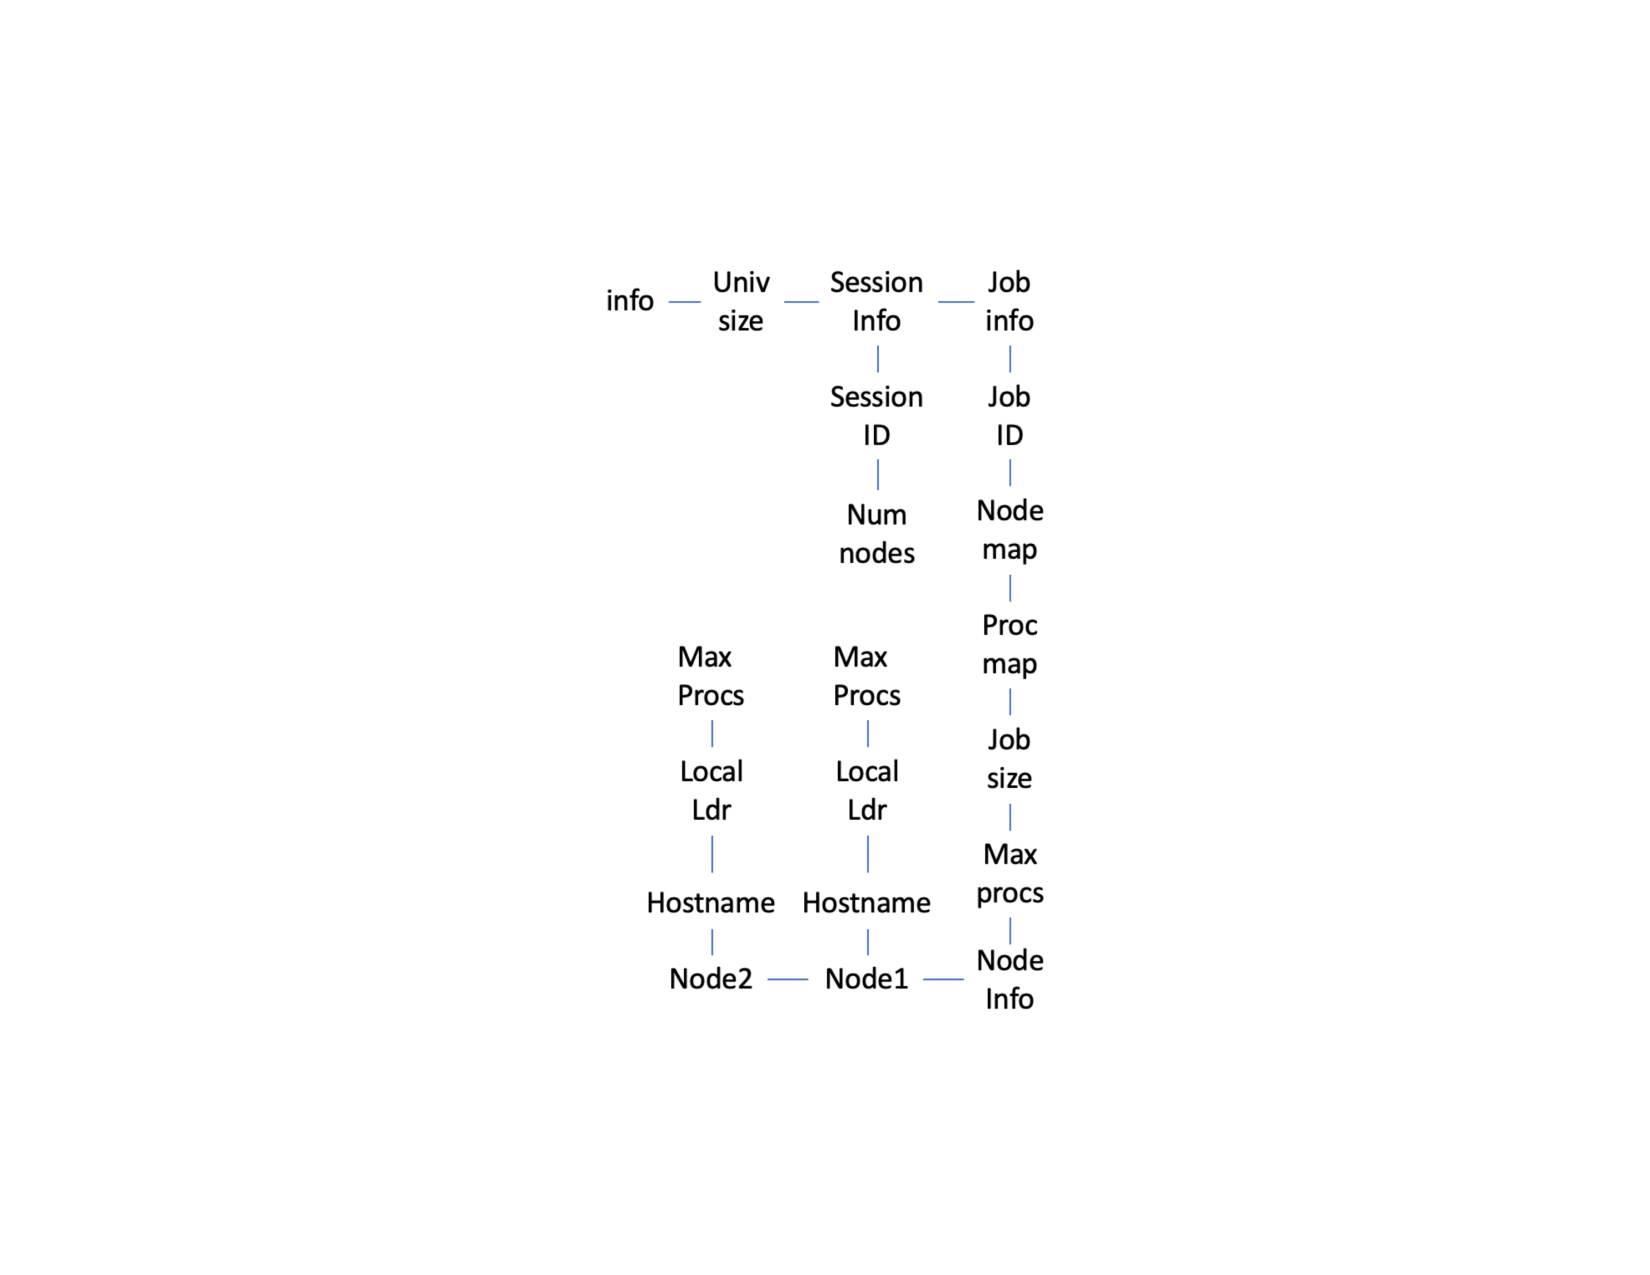
\includegraphics[clip,width=0.4\textwidth]{figs/jobinfo.pdf}
  \end{center}
  \caption{Job-level information elements}
  \label{fig:jobinfo}
\end{figure*}
\endgroup

Note that in this example, \refattr{PMIX_NUM_NODES} is not required as that information is contained in the \refattr{PMIX_NODE_MAP} attribute. Similarly, \refattr{PMIX_JOB_SIZE} is not technically required as that information is contained in the \refattr{PMIX_PROC_MAP} when combined with the corresponding node map - however, there is no issue with including the job size as a separate entry.

The example also illustrates the hierarchical use of the \refattr{PMIX_NODE_INFO_ARRAY} attribute. In this case, we have chosen to pass several job-related values for each node - since those values are non-unique across the job, they must be passed in a node-info container. Note that the choice of what information to pass into the \ac{PMIx} server library versus what information to derive from other values at time of request is left to the host environment. \ac{PMIx} implementors in turn may, if they choose, pre-parse registration data to create expanded views (thus enabling faster response to requests at the expense of memory footprint) or to compress views into tighter representations (thus trading minimized footprint for longer response times).

\item Application-level information includes all application-specific values such as \refattr{PMIX_APP_SIZE} and \refattr{PMIX_APPLDR}. If the \refterm{job} contains only a single \refterm{application}, then the application-specific values can be specified independently - i.e., in their own \refstruct{pmix_info_t} elements of the \refarg{info} array - or as a \refstruct{pmix_data_array_t} array of \refstruct{pmix_info_t} using the \refattr{PMIX_APP_INFO_ARRAY} attribute and identifed by including the \refattr{PMIX_APPNUM} attribute in the array. Use of the array format is  must in cases where non-specific attributes (e.g., \refattr{PMIX_NODE_MAP}) are passed to describe aspects of the application.

However, in the case of a job consisting of multiple applications, all application-specific values for each application must be provided using the \refattr{PMIX_APP_INFO_ARRAY} format, each identified by its \refattr{PMIX_APPNUM} value.

Upon conclusion of this step, the \refarg{info} array might look like that shown in \ref{fig:appinfo}, assuming there are two applications in the job being registered:

\begingroup
\begin{figure*}[ht!]
  \begin{center}
    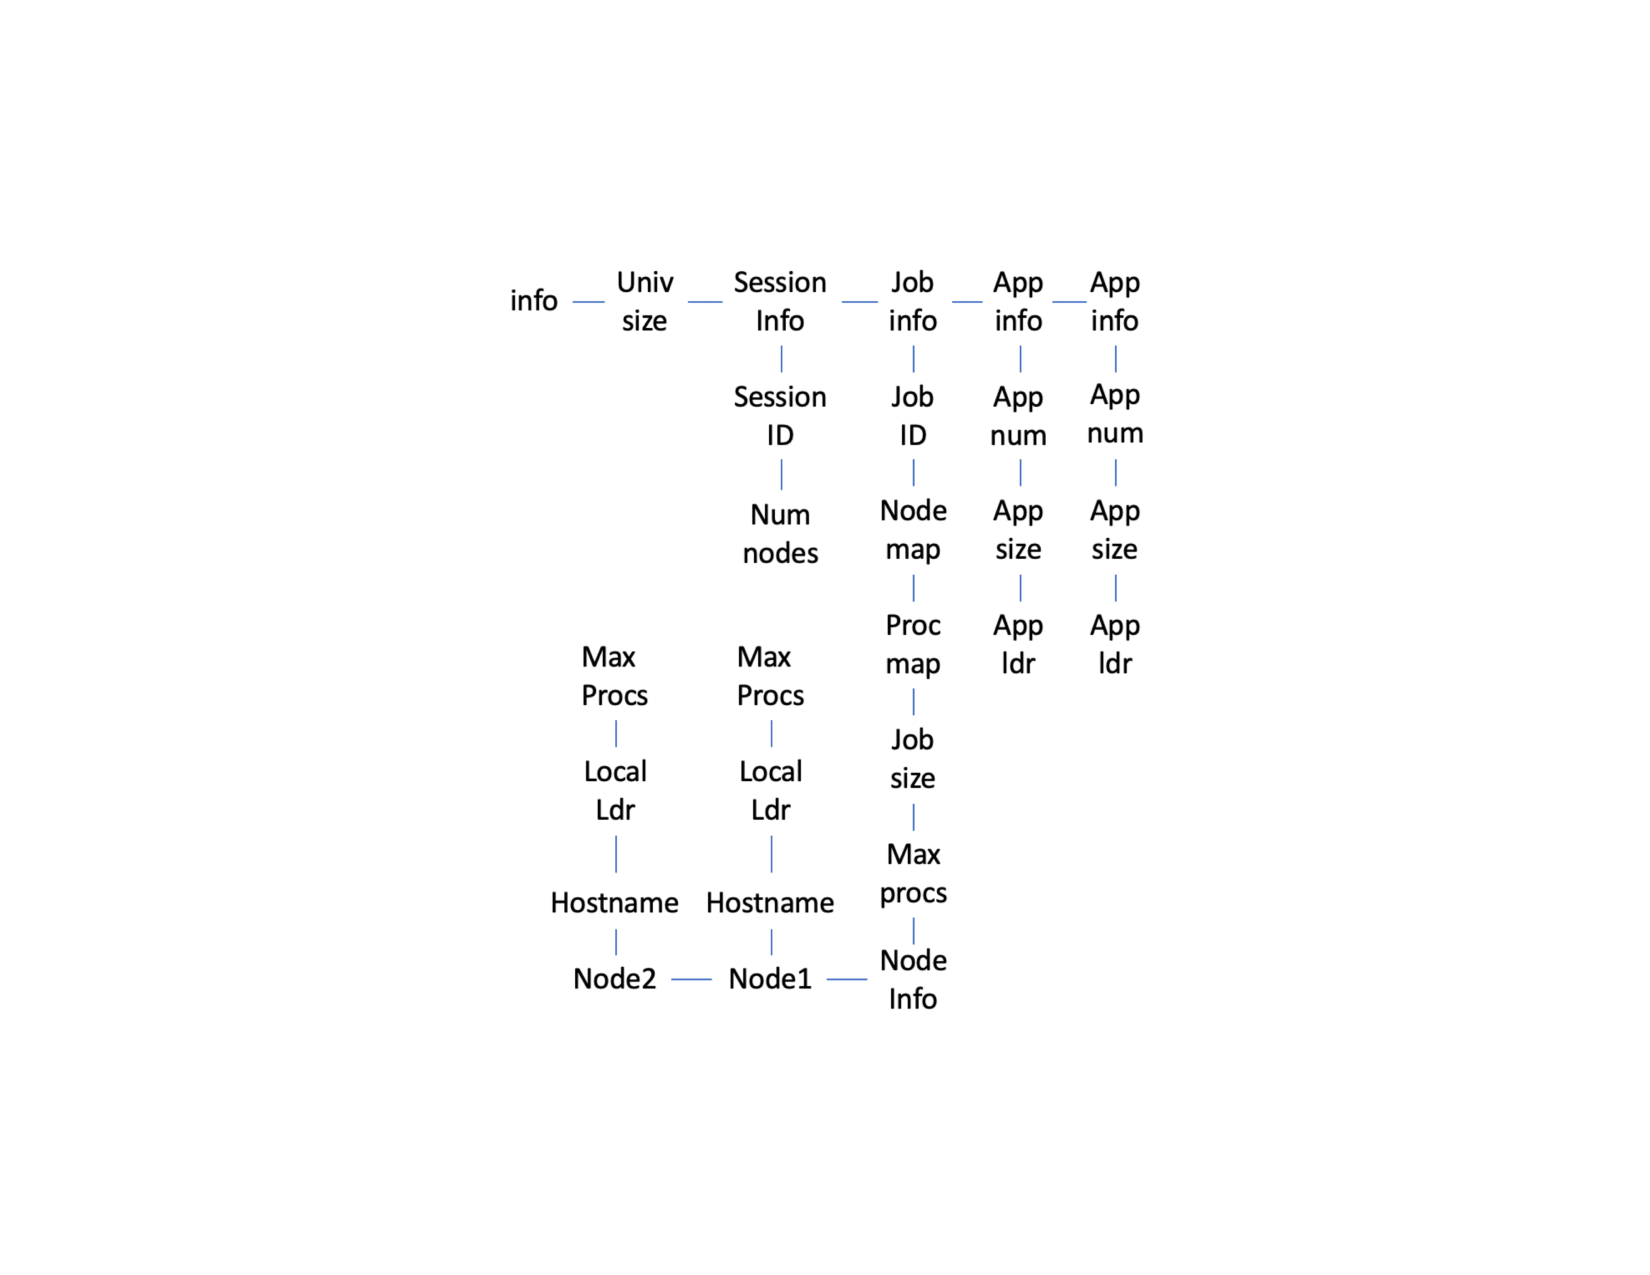
\includegraphics[clip,width=0.5\textwidth]{figs/appinfo.pdf}
  \end{center}
  \caption{Application-level information elements}
  \label{fig:appinfo}
\end{figure*}
\endgroup

\item Process-level information includes an entry for each process in the job being registered, each entry marked with the \refattr{PMIX_PROC_INFO_ARRAY} attribute. The \refterm{rank} of the process must be the first entry in the array - this provides efficiency when storing the data. Upon conclusion of this step, the \refarg{info} array might look like the diagram in \ref{fig:procinfo}:

\begingroup
\begin{figure*}[ht!]
  \begin{center}
    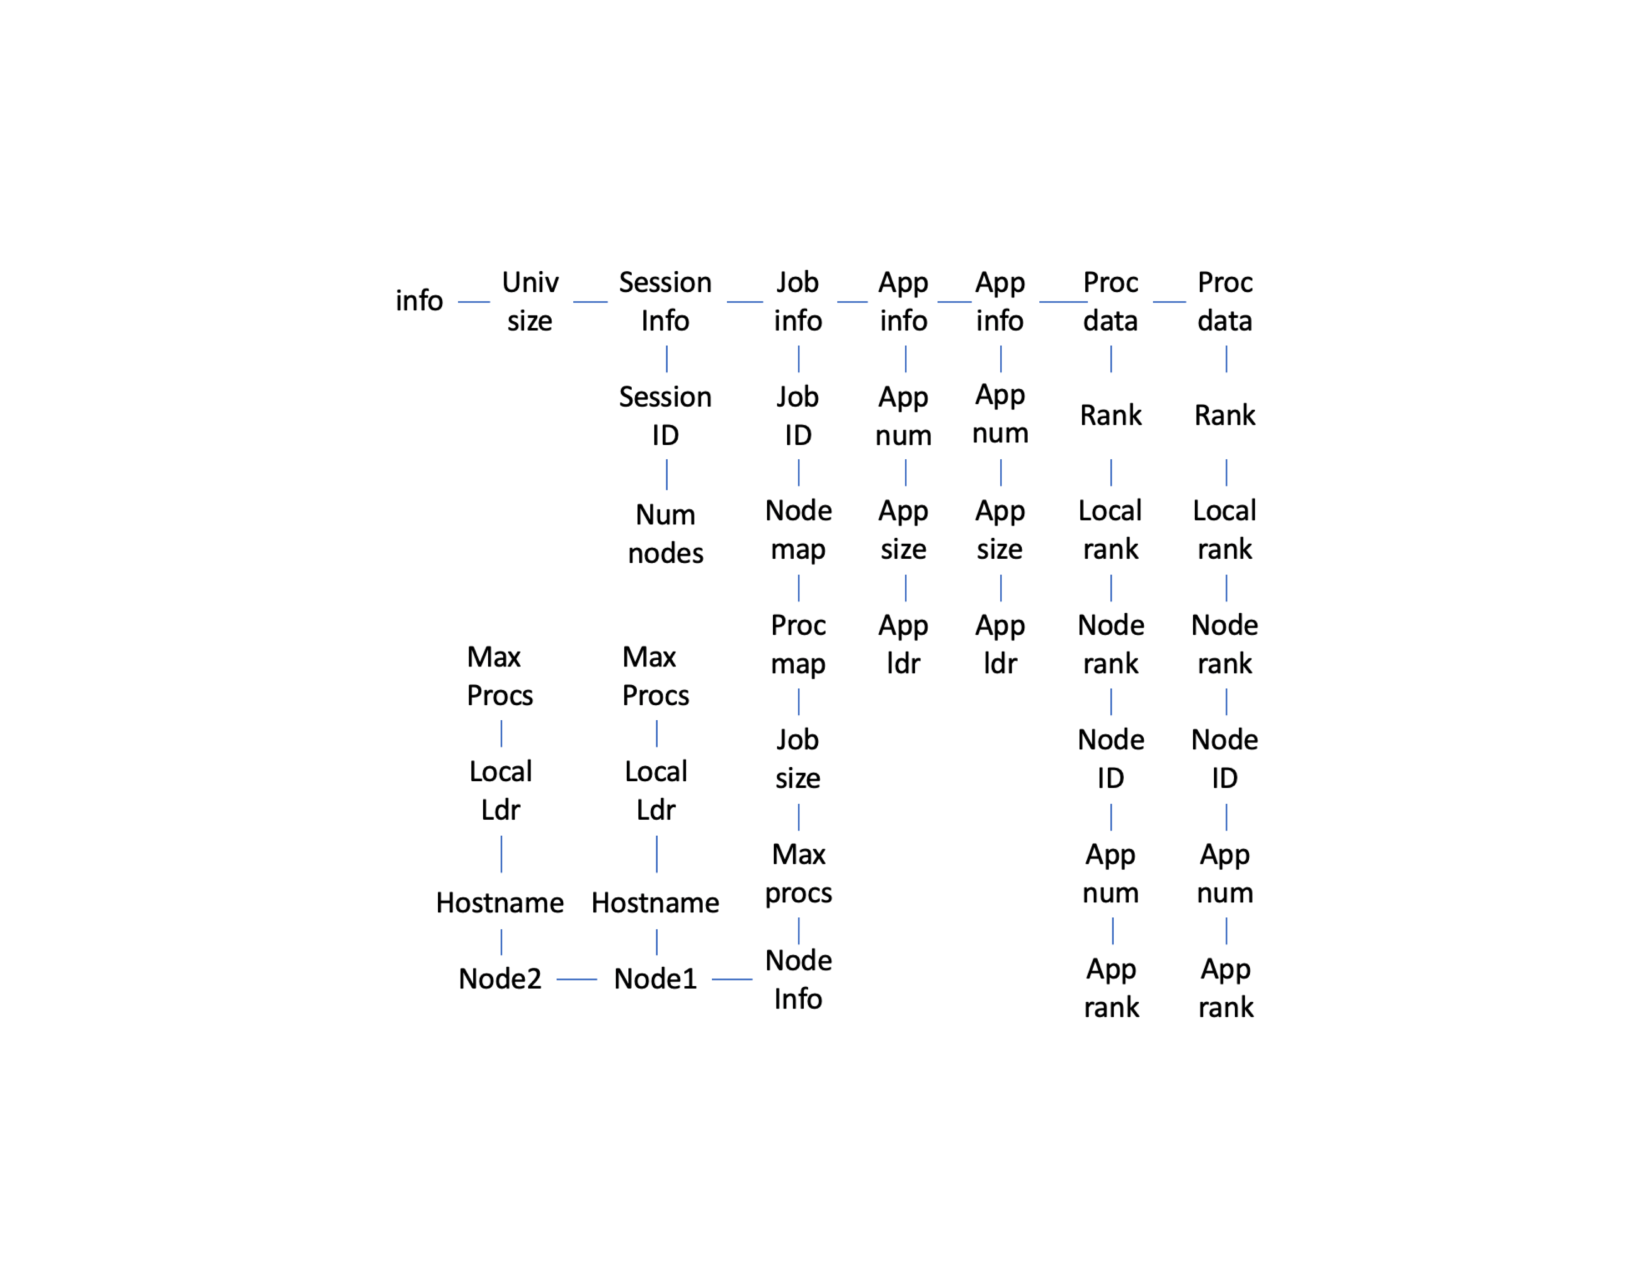
\includegraphics[clip,width=0.8\textwidth]{figs/procinfo.pdf}
  \end{center}
  \caption{Process-level information elements}
  \label{fig:procinfo}
\end{figure*}
\endgroup

\item For purposes of this example, node-level information only includes values describing the local node - i.e., it does not include information about other nodes in the job or session. In many cases, the values included in this level are unique to it and can be specified independently - i.e., in their own \refstruct{pmix_info_t} elements of the \refarg{info} array. Alternatively, they can be provided as a \refstruct{pmix_data_array_t} array of \refstruct{pmix_info_t} using the \refattr{PMIX_NODE_INFO_ARRAY} attribute - this is required in cases where non-specific attributes are passed to describe aspects of the node, or where values for multiple nodes are being provided.

The node-level information requires two elements that must be constructed in a manner similar to that used for the node map. The \refattr{PMIX_LOCAL_PEERS} value is computed based on the processes on the local node, filtered to select those from the job being registered, as shown below using the tools provided by \ac{PMIx}:

\cspecificstart
\begin{codepar}
char **ndppn = NULL;
char rank[30];
char *localranks;
size_t m;
pmix_info_t info;

for (m=0; m < mynode->num_procs; m++) \{
    /* ignore processes that are not part of the target job */
    if (!PMIX_CHECK_NSPACE(targetjob,mynode->proc[m].nspace)) \{
        continue;
    \}
    snprintf(rank, 30, "%d", mynode->proc[m].rank);
    PMIX_ARGV_APPEND(&ndppn, rank);
\}
/* convert the array into a comma-delimited string of ranks */
localranks = PMIX_ARGV_JOIN(ndppn, ',');
/* release the local array */
PMIX_ARGV_FREE(ndppn);

/* pass the string as the value to the PMIX_LOCAL_PEERS key */
PMIX_INFO_LOAD(&info, PMIX_LOCAL_PEERS, localranks, PMIX_STRING);

/* release the list */
free(localranks);
\end{codepar}
\cspecificend

The \refattr{PMIX_LOCAL_CPUSETS} value is constructed in a similar manner. In the provided example, it is assumed that an \ac{HWLOC} cpuset representation (a comma-delimited string of processor IDs) of the processors assigned to each process has previously been generated and stored on the process description. Thus, the value can be constructed as shown below:

\cspecificstart
\begin{codepar}
char **ndcpus = NULL;
char *localcpus;
size_t m;
pmix_info_t info;

for (m=0; m < mynode->num_procs; m++) \{
    /* ignore processes that are not part of the target job */
    if (!PMIX_CHECK_NSPACE(targetjob,mynode->proc[m].nspace)) \{
        continue;
    \}
    PMIX_ARGV_APPEND(&ndcpus, mynode->proc[m].cpuset);
\}
/* convert the array into a colon-delimited string */
localcpus = PMIX_ARGV_JOIN(ndcpus, ':');
/* release the local array */
PMIX_ARGV_FREE(ndcpus);

/* pass the string as the value to the PMIX_LOCAL_CPUSETS key */
PMIX_INFO_LOAD(&info, PMIX_LOCAL_CPUSETS, localcpus, PMIX_STRING);

/* release the list */
free(localcpus);
\end{codepar}
\cspecificend

Note that for efficiency, these two values can be computed at the same time.

\end{itemize}

The final \refarg{info} array might therefore look like the diagram in \ref{fig:nodeinfo}:

\begingroup
\begin{figure*}[ht!]
  \begin{center}
    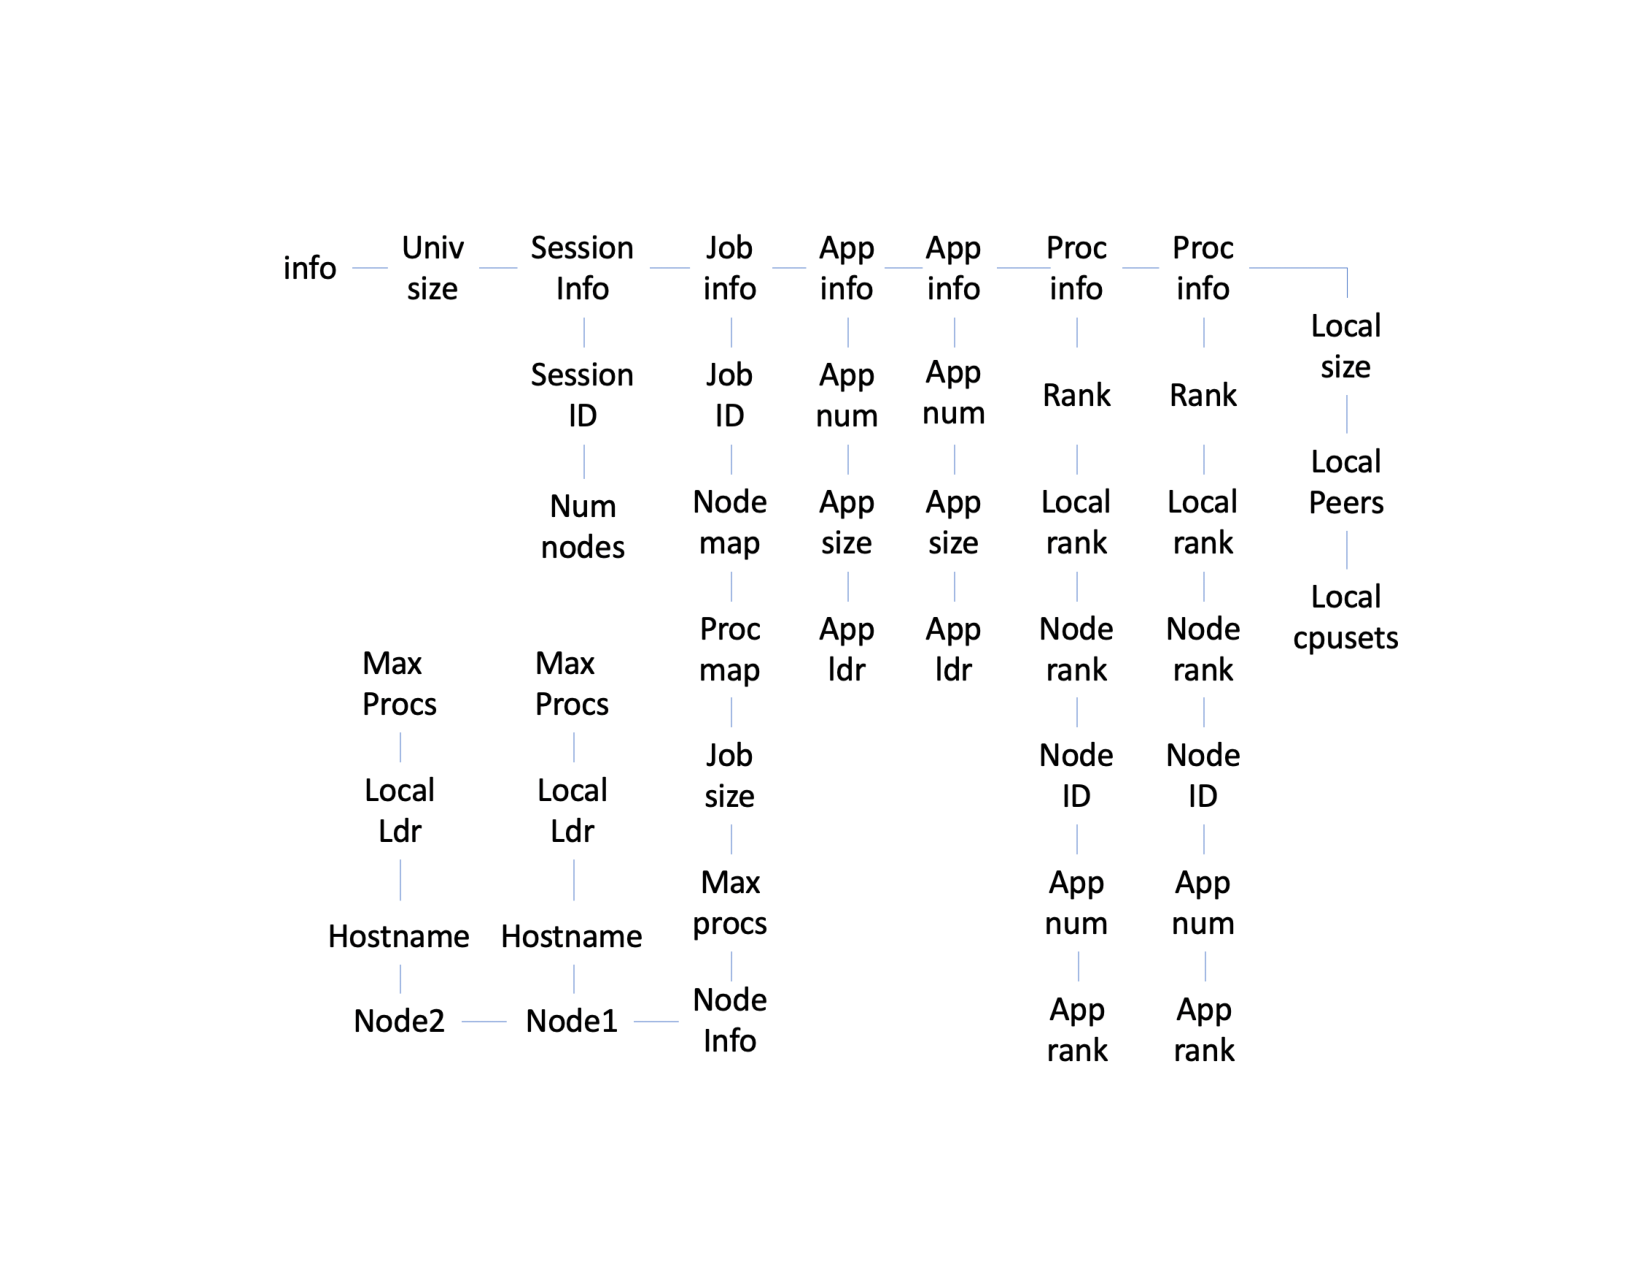
\includegraphics[clip,width=0.8\textwidth]{figs/nodeinfo.pdf}
  \end{center}
  \caption{Final information array}
  \label{fig:nodeinfo}
\end{figure*}
\endgroup


%%%%%%%%%%%%%%%%%%%%%%%%%%%%%%%%%%%%%%%%%%%%%%%%%
\subsection{\code{PMIx_server_deregister_nspace}}
\declareapi{PMIx_server_deregister_nspace}

%%%%
\summary

Deregister a namespace.

%%%%
\format

\versionMarker{1.0}
\cspecificstart
\begin{codepar}
void PMIx_server_deregister_nspace(const pmix_nspace_t nspace,
                        pmix_op_cbfunc_t cbfunc, void *cbdata);
\end{codepar}
\cspecificend

\begin{arglist}
\argin{nspace}{Namespace (string)}
\argin{cbfunc}{Callback function \refapi{pmix_op_cbfunc_t} (function reference)}
\argin{cbdata}{Data to be passed to the callback function (memory reference)}
\end{arglist}

%%%%
\descr

Deregister the specified \refarg{nspace} and purge all objects relating to it, including any client information from that namespace.
This is intended to support persistent \ac{PMIx} servers by providing an opportunity for the host \ac{RM} to tell the \ac{PMIx} server library to release all memory for a completed job. Note that the library must not invoke the callback function prior to returning from the \ac{API}.


%%%%%%%%%%%%%%%%%%%%%%%%%%%%%%%%%%%%%%%%%%%%%%%%%
\subsection{\code{PMIx_server_register_client}}
\declareapi{PMIx_server_register_client}

%%%%
\summary

Register a client process with the PMIx server library.

%%%%
\format

\versionMarker{1.0}
\cspecificstart
\begin{codepar}
pmix_status_t
PMIx_server_register_client(const pmix_proc_t *proc,
                        uid_t uid, gid_t gid,
                        void *server_object,
                        pmix_op_cbfunc_t cbfunc, void *cbdata);
\end{codepar}
\cspecificend

\begin{arglist}
\argin{proc}{\refstruct{pmix_proc_t} structure (handle)}
\argin{uid}{user id (integer)}
\argin{gid}{group id (integer)}
\argin{server_object}{(memory reference)}
\argin{cbfunc}{Callback function \refapi{pmix_op_cbfunc_t} (function reference)}
\argin{cbdata}{Data to be passed to the callback function (memory reference)}
\end{arglist}

Returns one of the following:

\begin{itemize}
    \item \refconst{PMIX_SUCCESS}, indicating that the request is being processed by the host environment - result will be returned in the provided \refarg{cbfunc}. Note that the library must not invoke the callback function prior to returning from the \ac{API}.
    \item \refconst{PMIX_OPERATION_SUCCEEDED}, indicating that the request was immediately processed and returned \textit{success} - the \refarg{cbfunc} will not be called
    \item a PMIx error constant indicating either an error in the input or that the request was immediately processed and failed - the \refarg{cbfunc} will not be called
\end{itemize}

%%%%
\descr

Register a client process with the PMIx server library.

The host server can also, if it desires, provide an object it wishes to be returned when a server function is called that relates to a specific process.
For example, the host server may have an object that tracks the specific client.
Passing the object to the library allows the library to provide that object to the host server during subsequent calls related to that client, such as a \refapi{pmix_server_client_connected_fn_t} function.  This allows the host server to access the object without performing a lookup based on the client's namespace and rank.

\advicermstart
Host environments are required to execute this operation prior to starting the client process.
The expected user ID and group ID of the child process allows the server library to properly authenticate clients as they connect by requiring the two values to match. Accordingly, the detected user and group ID's of the connecting process are not included in the \refapi{pmix_server_client_connected_fn_t} server module function.
\advicermend

\adviceimplstart
For security purposes, the \ac{PMIx} server library should check the user and group ID's of a connecting process against those provided for the declared client process identifier via the \refapi{PMIx_server_register_client} prior to completing the connection.
\adviceimplend


%%%%%%%%%%%%%%%%%%%%%%%%%%%%%%%%%%%%%%%%%%%%%%%%%
\subsection{\code{PMIx_server_deregister_client}}
\declareapi{PMIx_server_deregister_client}

%%%%
\summary

Deregister a client and purge all data relating to it.

%%%%
\format

\versionMarker{1.0}
\cspecificstart
\begin{codepar}
void
PMIx_server_deregister_client(const pmix_proc_t *proc,
                        pmix_op_cbfunc_t cbfunc, void *cbdata);
\end{codepar}
\cspecificend

\begin{arglist}
\argin{proc}{\refstruct{pmix_proc_t} structure (handle)}
\argin{cbfunc}{Callback function \refapi{pmix_op_cbfunc_t} (function reference)}
\argin{cbdata}{Data to be passed to the callback function (memory reference)}
\end{arglist}


%%%%
\descr

The \refapi{PMIx_server_deregister_nspace} \ac{API} will delete all client information for that namespace. The \ac{PMIx} server library will automatically perform that operation upon disconnect of all local clients.
This \ac{API} is therefore intended primarily for use in exception cases, but can be called in non-exception cases if desired. Note that the library must not invoke the callback function prior to returning from the \ac{API}.


%%%%%%%%%%%%%%%%%%%%%%%%%%%%%%%%%%%%%%%%%%%%%%%%%
\subsection{\code{PMIx_server_setup_fork}}
\declareapi{PMIx_server_setup_fork}

%%%%
\summary

Setup the environment of a child process to be forked by the host.

%%%%
\format

\versionMarker{1.0}
\cspecificstart
\begin{codepar}
pmix_status_t
PMIx_server_setup_fork(const pmix_proc_t *proc,
                        char ***env);
\end{codepar}
\cspecificend

\begin{arglist}
\argin{proc}{\refstruct{pmix_proc_t} structure (handle)}
\argin{env}{Environment array (array of strings)}
\end{arglist}

Returns \refconst{PMIX_SUCCESS} or a negative value corresponding to a PMIx error constant.

%%%%
\descr

Setup the environment of a child process to be forked by the host so it can correctly interact with the PMIx server.

The \ac{PMIx} client needs some setup information so it can properly connect back to the server.
This function will set appropriate environmental variables for this purpose, and will also provide any environmental variables that were specified in the launch command (e.g., via \refapi{PMIx_Spawn}) plus other values (e.g., variables required to properly initialize the client's fabric library).

\advicermstart
Host environments are required to execute this operation prior to starting the client process.
\advicermend


%%%%%%%%%%%%%%%%%%%%%%%%%%%%%%%%%%%%%%%%%%%%%%%%%
\subsection{\code{PMIx_server_dmodex_request}}
\declareapi{PMIx_server_dmodex_request}

%%%%
\summary

Define a function by which the host server can request modex data from the local PMIx server.

%%%%
\format

\versionMarker{1.0}
\cspecificstart
\begin{codepar}
pmix_status_t
PMIx_server_dmodex_request(const pmix_proc_t *proc,
                           pmix_dmodex_response_fn_t cbfunc,
                           void *cbdata);
\end{codepar}
\cspecificend

\begin{arglist}
\argin{proc}{\refstruct{pmix_proc_t} structure (handle)}
\argin{cbfunc}{Callback function \refapi{pmix_dmodex_response_fn_t} (function reference)}
\argin{cbdata}{Data to be passed to the callback function (memory reference)}
\end{arglist}

Returns one of the following:

\begin{itemize}
    \item \refconst{PMIX_SUCCESS}, indicating that the request is being processed by the host environment - result will be returned in the provided \refarg{cbfunc}. Note that the library must not invoke the callback function prior to returning from the \ac{API}.
    \item a PMIx error constant indicating an error in the input - the \refarg{cbfunc} will not be called
\end{itemize}


%%%%
\descr

Define a function by which the host server can request modex data from the local \ac{PMIx} server. Traditional wireup procedures revolve around the per-process posting of data (e.g., location and endpoint information) via the \refapi{PMIx_Put} and \refapi{PMIx_Commit} functions followed by a \refapi{PMIx_Fence} barrier that globally exchanges the posted information. However, the barrier operation represents a signficant time impact at large scale.

\ac{PMIx} supports an alternative wireup method known as \textit{Direct Modex} that replaces the barrier-based exchange of all process-posted information with on-demand fetch of a peer's data. In place of the barrier operation, data posted by each process is cached on the local \ac{PMIx} server. When a process requests the information posted by a particular peer, it first checks the local cache to see if the data is already available. If not, then the request is passed to the local \ac{PMIx} server, which subsequently requests that its \ac{RM} host request the data from the \ac{RM} daemon on the node where the specified peer process is located. Upon receiving the request, the \ac{RM} daemon passes the request into its \ac{PMIx} server library using the \refapi{PMIx_server_dmodex_request} function, receiving the response in the provided \refarg{cbfunc} once the indicated process has posted its information. The \ac{RM} daemon then returns the data to the requesting daemon, who subsequently passes the data to its \ac{PMIx} server library for transfer to the requesting client.

\adviceuserstart
While direct modex allows for faster launch times by eliminating the barrier operation, per-peer retrieval of posted information is less efficient. Optimizations can be implemented - e.g., by returning posted information from all processes on a node upon first request - but in general direct modex remains best suited for sparsely connected applications.
\adviceuserend

%%%%%%%%%%%%%%%%%%%%%%%%%%%%%%%%%%%%%%%%%%%%%%%%%
\subsubsection{Server Direct Modex Response Callback Function}
\declareapi{pmix_dmodex_response_fn_t}

The \refapi{PMIx_server_dmodex_request} callback function.

%%%%
\summary

Provide a function by which the local \ac{PMIx} server library can return connection and other data posted by local application processes to the host resource manager.

%%%%
\format

\versionMarker{1.0}
\cspecificstart
\begin{codepar}
typedef void (*pmix_dmodex_response_fn_t)(
                    pmix_status_t status,
                    char *data, size_t sz,
                    void *cbdata);
\end{codepar}
\cspecificend

\begin{arglist}
\argin{status}{Returned status of the request (\refstruct{pmix_status_t})}
\argin{data}{Pointer to a data "blob" containing the requested information (handle)}
\argin{sz}{Number of bytes in the \refarg{data} blob (integer)}
\argin{cbdata}{Data passed into the initial call to \refapi{PMIx_server_dmodex_request} (memory reference)}
\end{arglist}

\descr
Define a function to be called by the PMIx server library for return of information posted by a local application process (via \refapi{PMIx_Put} with subsequent \refapi{PMIx_Commit}) in response to a request from the host RM. The returned \refarg{data} blob is owned by the PMIx server library and will be free’d upon return from the function.


%%%%%%%%%%%%%%%%%%%%%%%%%%%%%%%%%%%%%%%%%%%%%%%%%
\subsection{\code{PMIx_server_setup_application}}
\declareapi{PMIx_server_setup_application}

%%%%
\summary

Provide a function by which a launcher can request application-specific setup data prior to launch of a \refterm{job}.

%%%%
\format

\versionMarker{2.0}
\cspecificstart
\begin{codepar}
pmix_status_t
PMIx_server_setup_application(const pmix_nspace_t nspace,
                        pmix_info_t info[], size_t ninfo,
                        pmix_setup_application_cbfunc_t cbfunc,
                        void *cbdata);
\end{codepar}
\cspecificend

\begin{arglist}
\argin{nspace}{namespace (string)}
\argin{info}{Array of info structures (array of handles)}
\argin{ninfo}{Number of elements in the \refarg{info} array (integer)}
\argin{cbfunc}{Callback function \refapi{pmix_setup_application_cbfunc_t} (function reference)}
\argin{cbdata}{Data to be passed to the \refarg{cbfunc} callback function (memory reference)}
\end{arglist}

Returns one of the following:

\begin{itemize}
    \item \refconst{PMIX_SUCCESS}, indicating that the request is being processed by the host environment - result will be returned in the provided \refarg{cbfunc}. Note that the library must not invoke the callback function prior to returning from the \ac{API}.
    \item a PMIx error constant indicating either an error in the input - the \refarg{cbfunc} will not be called
\end{itemize}


\reqattrstart
\ac{PMIx} libraries that support this operation are required to support the following:

\pasteAttributeItem{PMIX_SETUP_APP_ENVARS}
\pasteAttributeItem{PMIX_SETUP_APP_NONENVARS}
\pasteAttributeItem{PMIX_SETUP_APP_ALL}
\pasteAttributeItem{PMIX_ALLOC_FABRIC}
\pasteAttributeItem{PMIX_ALLOC_FABRIC_ID}
\pasteAttributeItem{PMIX_ALLOC_FABRIC_SEC_KEY}
\pasteAttributeItem{PMIX_ALLOC_FABRIC_TYPE}
\pasteAttributeItem{PMIX_ALLOC_FABRIC_PLANE}
\pasteAttributeItem{PMIX_ALLOC_FABRIC_ENDPTS}
\pasteAttributeItem{PMIX_ALLOC_FABRIC_ENDPTS_NODE}
\pasteAttributeItem{PMIX_PROC_MAP}
\pasteAttributeItem{PMIX_NODE_MAP}

\reqattrend

\optattrstart
\ac{PMIx} libraries that support this operation may support the following:

\pasteAttributeItem{PMIX_ALLOC_BANDWIDTH}
\pasteAttributeItem{PMIX_ALLOC_FABRIC_QOS}

The following optional attributes may be provided by the host environment to identify the programming model (as specified by the user) being executed within the application. The \ac{PMIx} server library may utilize this information to harvest/forward model-specific environmental variables, record the programming model associated with the application, etc.

\begin{itemize}
    \item \pasteAttributeItem{PMIX_PROGRAMMING_MODEL}
    \item \pasteAttributeItem{PMIX_MODEL_LIBRARY_NAME}
    \item \pasteAttributeItem{PMIX_MODEL_LIBRARY_VERSION}
\end{itemize}

\optattrend

%%%%
\descr

Provide a function by which the \ac{RM} can request application-specific setup data (e.g., environmental variables, fabric configuration and security credentials) from supporting \ac{PMIx} server library subsystems prior to initiating launch of a job.

This is defined as a non-blocking operation in case contributing subsystems need to perform some potentially time consuming action (e.g., query a remote service) before responding. The returned data must be distributed by the host environment and subsequently delivered to the local \ac{PMIx} server on each node where application processes will execute, prior to initiating execution of those processes.

\advicermstart
Host environments are required to execute this operation prior to launching a job. In addition to supported directives, the \refarg{info} array must include a description of the \refterm{job} using the \refattr{PMIX_NODE_MAP} and \refattr{PMIX_PROC_MAP} attributes.

Note that the function can be called on a per-application basis if the \refattr{PMIX_PROC_MAP} and \refattr{PMIX_NODE_MAP} are provided only for the corresponding application (as opposed to the entire job) each time.
\advicermend

\adviceimplstart
Support for harvesting of environmental variables and providing of local configuration information by the \ac{PMIx} implementation is optional.
\adviceimplend

%%%%%%%%%%%%%%%%%%%%%%%%%%%%%%%%%%%%%%%%%%%%%%%%%
\subsubsection{Server Setup Application Callback Function}
\declareapi{pmix_setup_application_cbfunc_t}

The \refapi{PMIx_server_setup_application} callback function.

%%%%
\summary

Provide a function by which the resource manager can receive application-specific environmental variables and other setup data prior to launch of an application.

%%%%
\format

\versionMarker{2.0}
\cspecificstart
\begin{codepar}
typedef void (*pmix_setup_application_cbfunc_t)(
                        pmix_status_t status,
                        pmix_info_t info[], size_t ninfo,
                        void *provided_cbdata,
                        pmix_op_cbfunc_t cbfunc, void *cbdata);
\end{codepar}
\cspecificend

\begin{arglist}
\argin{status}{returned status of the request (\refstruct{pmix_status_t})}
\argin{info}{Array of info structures (array of handles)}
\argin{ninfo}{Number of elements in the \refarg{info} array (integer)}
\argin{provided_cbdata}{Data originally passed to call to \refapi{PMIx_server_setup_application} (memory reference)}
\argin{cbfunc}{\refapi{pmix_op_cbfunc_t} function to be called when processing completed (function reference)}
\argin{cbdata}{Data to be passed to the \refarg{cbfunc} callback function (memory reference)}
\end{arglist}

\descr

Define a function to be called by the \ac{PMIx} server library for return of application-specific setup data in response to a request from the host \ac{RM}. The returned \refarg{info} array is owned by the \ac{PMIx} server library and will be free'd when the provided \refarg{cbfunc} is called.


%%%%%%%%%%%%%%%%%%%%%%%%%%%%%%%%%%%%%%%%%%%%%%%%%
\subsubsection{Server Setup Application Attributes}
\label{api:struct:attributes:security}

\versionMarker{3.0}
Attributes specifically defined for controlling contents of application setup data.

%
\declareAttribute{PMIX_SETUP_APP_ENVARS}{"pmix.setup.env"}{bool}{
Harvest and include relevant environmental variables.
}
%
\declareAttribute{PMIX_SETUP_APP_NONENVARS}{""pmix.setup.nenv"}{bool}{
Include all relevant data other than environmental variables.
}
%
\declareAttribute{PMIX_SETUP_APP_ALL}{"pmix.setup.all"}{bool}{
Include all relevant data.
}


%%%%%%%%%%%%%%%%%%%%%%%%%%%%%%%%%%%%%%%%%%%%%%%%%
\subsection{\code{PMIx_Register_attributes}}
\declareapi{PMIx_Register_attributes}

%%%%
\summary

Register host environment attribute support for a function.

%%%%
\format

\versionMarker{4.0}
\cspecificstart
\begin{codepar}
pmix_status_t
PMIx_Register_attributes(char *function,
                         pmix_regattr_t attrs[],
                         size_t nattrs);
\end{codepar}
\cspecificend

\begin{arglist}
\argin{function}{String name of function (string)}
\argin{attrs}{Array of \refstruct{pmix_regattr_t} describing the supported attributes (handle)}
\argin{nattrs}{Number of elements in \refarg{attrs} (\code{size_t})}
\end{arglist}

Returns \refconst{PMIX_SUCCESS} or a negative value corresponding to a PMIx error constant.

%%%%
\descr

The \code{PMIx_Register_attributes} function is used by the host environment to register with its \ac{PMIx} server library the attributes it supports for each \refapi{pmix_server_module_t} function. The \refarg{function} is the string name of the server module function (e.g., "register_events", "validate_credential", or "allocate") whose attributes are being registered. See the \refstruct{pmix_regattr_t} entry for a description of the \refarg{attrs} array elements.

Note that the host environment can also query the library (using the \refapi{PMIx_Query_info_nb} \ac{API}) for its attribute support both at the server, client, and tool levels once the host has executed \refapi{PMIx_server_init} since the server will internally register those values.

\advicermstart
Host environments are strongly encouraged to register all supported attributes immediately after initializing the library to ensure that user requests are correctly serviced.
\advicermend

\adviceimplstart
\ac{PMIx} implementations are \emph{required} to register all internally supported attributes for each \ac{API} during initialization of the library (i.e., when the process calls their respective \ac{PMIx} init function). Specifically, the implementation \emph{must not} register supported attributes upon first call to a given \ac{API} as this would prevent users from discovering supported attributes prior to first use of an \ac{API}.

It is the implementation's responsibility to associate registered attributes for a given \refapi{pmix_server_module_t} function with their corresponding user-facing \ac{API}. Supported attributes \emph{must} be reported to users in terms of their support for user-facing \acp{API}, broken down by the level (see Section \ref{api:struct:attributes:query}) at which the attribute is supported.

Note that attributes can/will be registered on an \ac{API} for each level. It is \emph{required} that the implementation support user queries for supported attributes on a per-level basis. Duplicate registrations at the \emph{same} level for a function \emph{shall} return an error - however, duplicate registrations at \emph{different} levels \emph{shall} be independently tracked.
\adviceimplend


%%%%%%%%%%%%%%%%%%%%%%%%%%%%%%%%%%%%%%%%%%%%%%%%%
\subsubsection{Attribute registration constants}

Constants supporting attribute registration.

\begin{constantdesc}
%
\declareconstitemNEW{PMIX_ERR_REPEAT_ATTR_REGISTRATION}
The attributes for an identical function have already been registered at the specified level (host, server, or client).
%
\end{constantdesc}

%%%%%%%%%%%%%%%%%%%%%%%%%%%%%%%%%%%%%%%%%%%%%%%%%
\subsubsection{Attribute registration structure}
\declarestruct{pmix_regattr_t}

The \refstruct{pmix_regattr_t} structure is used to register attribute support for a \ac{PMIx} function.

\versionMarker{4.0}
\cspecificstart
\begin{codepar}
typedef struct pmix_regattr \{
    char *name;
    pmix_key_t *string;
    pmix_data_type_t type;
    pmix_info_t *info;
    size_t ninfo;
    char **description;
\} pmix_regattr_t;;
\end{codepar}
\cspecificend

Note that in this structure:

\begin{itemize}
    \item the \refarg{name} is the actual name of the attribute - e.g., "PMIX_MAX_PROCS"
    \item the \refarg{string} is the literal string value of the attribute - e.g., "pmix.max.size" for the \refattr{PMIX_MAX_PROCS} attribute
    \item \refarg{type} must be a \ac{PMIx} data type identifying the type of data associated with this attribute.
    \item the \refarg{info} array contains machine-usable information regarding the range of accepted values. This may include entries for \refattr{PMIX_MIN_VALUE}, \refattr{PMIX_MAX_VALUE}, \refattr{PMIX_ENUM_VALUE}, or a combination of them. For example, an attribute that supports all positive integers might delineate it by including a \refstruct{pmix_info_t} with a key of \refattr{PMIX_MIN_VALUE}, type of \refconst{PMIX_INT}, and value of zero. The lack of an entry for \refattr{PMIX_MAX_VALUE} indicates that there is no ceiling to the range of accepted values.
    \item \refarg{ninfo} indicates the number of elements in the \refarg{info} array
    \item The \refarg{description} field consists of a \code{NULL}-terminated array of strings describing the attribute, optionally including a human-readable description of the range of accepted values - e.g., "ALL POSITIVE INTEGERS", or a comma-delimited list of enum value names. No correlation between the number of entries in the \refarg{description} and the number of elements in the \refarg{info} array is implied or required.
\end{itemize}

The attribute \refarg{name} and \refarg{string} fields must be \code{NULL}-terminated strings composed of standard alphanumeric values supported by common utilities such as \textit{strcmp}.

Although not strictly required, both \ac{PMIx} library implementers and host environments are strongly encouraged to provide both human-readable and machine-parsable descriptions of supported attributes when registering them.

%%%%%%%%%%%%%%%%%%%%%%%%%%%%%%%%%%%%%%%%%%%%%%%%%
\subsubsection{Attribute registration structure descriptive attributes}
\label{api:struct:attributes:descr}

The following attributes relate to the nature of the values being reported
in the \refstruct{pmix_regattr_t} structures.

\declareAttributeNEW{PMIX_MAX_VALUE}{"pmix.descr.maxval"}{varies}{
Used in \refstruct{pmix_regattr_t} to describe the maximum valid value for the associated attribute.
}
%
\declareAttributeNEW{PMIX_MIN_VALUE}{"pmix.descr.minval"}{varies}{
Used in \refstruct{pmix_regattr_t} to describe the minimum valid value for the associated attribute.
}
%
\declareAttributeNEW{PMIX_ENUM_VALUE}{"pmix.descr.enum"}{char*}{
Used in \refstruct{pmix_regattr_t} to describe accepted values for the associated attribute. Numerical values shall be presented in a form convertible to the attribute's declared data type. Named values (i.e., values defined by constant names via a typical C-language enum declaration) must be provided as their numerical equivalent.
}

%%%%%%%%%%%%%%%%%%%%%%%%%%%%%%%%%%%%%%%%%%%%%%%%%
\subsubsection{Attribute registration structure support macros}

The following macros are provided to support the \refstruct{pmix_regattr_t} structure.

%%%%%%%%%%%
\littleheader{Initialize the regattr structure}
\declaremacro{PMIX_REGATTR_CONSTRUCT}

Initialize the \refstruct{pmix_regattr_t} fields

\versionMarker{4.0}
\cspecificstart
\begin{codepar}
PMIX_REGATTR_CONSTRUCT(m)
\end{codepar}
\cspecificend

\begin{arglist}
\argin{m}{Pointer to the structure to be initialized (pointer to \refstruct{pmix_regattr_t})}
\end{arglist}

%%%%%%%%%%%
\littleheader{Destruct the regattr structure}
\declaremacro{PMIX_REGATTR_DESTRUCT}

Destruct the \refstruct{pmix_regattr_t} fields, releasing all strings.

\versionMarker{4.0}
\cspecificstart
\begin{codepar}
PMIX_REGATTR_DESTRUCT(m)
\end{codepar}
\cspecificend

\begin{arglist}
\argin{m}{Pointer to the structure to be destructed (pointer to \refstruct{pmix_regattr_t})}
\end{arglist}

%%%%%%%%%%%
\littleheader{Create a regattr array}
\declaremacro{PMIX_REGATTR_CREATE}

Allocate and initialize an array of \refstruct{pmix_regattr_t} structures.

\versionMarker{4.0}
\cspecificstart
\begin{codepar}
PMIX_REGATTR_CREATE(m, n)
\end{codepar}
\cspecificend

\begin{arglist}
\arginout{m}{Address where the pointer to the array of \refstruct{pmix_regattr_t} structures shall be stored (handle)}
\argin{n}{Number of structures to be allocated (\code{size_t})}
\end{arglist}

%%%%%%%%%%%
\littleheader{Free a regattr array}
\declaremacro{PMIX_REGATTR_FREE}

Release an array of \refstruct{pmix_regattr_t} structures.

\versionMarker{4.0}
\cspecificstart
\begin{codepar}
PMIX_REGATTR_FREE(m, n)
\end{codepar}
\cspecificend

\begin{arglist}
\arginout{m}{Pointer to the array of \refstruct{pmix_regattr_t} structures (handle)}
\argin{n}{Number of structures in the array (\code{size_t})}
\end{arglist}

%%%%%%%%%%%
\littleheader{Load a regattr structure}
\declaremacro{PMIX_REGATTR_LOAD}

Load values into a \refstruct{pmix_regattr_t} structure. The macro can be called multiple times to add as many strings as desired to the same structure by passing the same address and a \code{NULL} key to the macro. Note that the \refarg{t} type value must be given each time.

\versionMarker{4.0}
\cspecificstart
\begin{codepar}
PMIX_REGATTR_LOAD(a, n, k, t, ni, v)
\end{codepar}
\cspecificend

\begin{arglist}
\argin{a}{Pointer to the structure to be loaded (pointer to \refstruct{pmix_proc_t})}
\argin{n}{String name of the attribute (string)}
\argin{k}{Key value to be loaded (\refstruct{pmix_key_t})}
\argin{t}{Type of data associated with the provided key (\refstruct{pmix_data_type_t})}
\argin{ni}{Number of \refstruct{pmix_info_t} elements to be allocated in \refarg{info} (\code{size_t})}
\argin{v}{One-line description to be loaded (more can be added separately) (string)}
\end{arglist}

%%%%%%%%%%%
\littleheader{Transfer a regattr to another regattr}
\declaremacro{PMIX_REGATTR_XFER}

Non-destructively transfer the contents of a \refstruct{pmix_regattr_t} structure to another one.

\versionMarker{4.0}
\cspecificstart
\begin{codepar}
PMIX_REGATTR_XFER(m, n)
\end{codepar}
\cspecificend

\begin{arglist}
\arginout{m}{Pointer to the destination \refstruct{pmix_regattr_t} structure (handle)}
\argin{m}{Pointer to the source \refstruct{pmix_regattr_t} structure (handle)}
\end{arglist}


%%%%%%%%%%%%%%%%%%%%%%%%%%%%%%%%%%%%%%%%%%%%%%%%%
\subsection{\code{PMIx_server_setup_local_support}}
\declareapi{PMIx_server_setup_local_support}

%%%%
\summary

Provide a function by which the local \ac{PMIx} server can perform any application-specific operations prior to spawning local clients of a given application.

%%%%
\format

\versionMarker{2.0}
\cspecificstart
\begin{codepar}
pmix_status_t
PMIx_server_setup_local_support(const pmix_nspace_t nspace,
                                pmix_info_t info[], size_t ninfo,
                                pmix_op_cbfunc_t cbfunc,
                                void *cbdata);
\end{codepar}
\cspecificend

\begin{arglist}
\argin{nspace}{Namespace (string)}
\argin{info}{Array of info structures (array of handles)}
\argin{ninfo}{Number of elements in the \refarg{info} array (\code{size_t})}
\argin{cbfunc}{Callback function \refapi{pmix_op_cbfunc_t} (function reference)}
\argin{cbdata}{Data to be passed to the callback function (memory reference)}
\end{arglist}

Returns one of the following:

\begin{itemize}
    \item \refconst{PMIX_SUCCESS}, indicating that the request is being processed by the host environment - result will be returned in the provided \refarg{cbfunc}. Note that the library must not invoke the callback function prior to returning from the \ac{API}.
    \item \refconst{PMIX_OPERATION_SUCCEEDED}, indicating that the request was immediately processed and returned \textit{success} - the \refarg{cbfunc} will not be called
    \item a PMIx error constant indicating either an error in the input or that the request was immediately processed and failed - the \refarg{cbfunc} will not be called
\end{itemize}


%%%%
\descr

Provide a function by which the local \ac{PMIx} server can perform any application-specific operations prior to spawning local clients of a given application. For example, a fabric library might need to setup the local driver for ``instant on'' addressing. The data provided in the \refarg{info} array is the data returned to the host \ac{RM} by the callback function executed as a result of a call to \refapi{PMIx_server_setup_application}.

\advicermstart
Host environments are required to execute this operation prior to starting any local application processes from the specified namespace if information was obtained from a call to \refapi{PMIx_server_setup_application}.
\advicermend

%%%%%%%%%%%%%%%%%%%%%%%%%%%%%%%%%%%%%%%%%%%%%%%%%
\subsection{\code{PMIx_server_IOF_deliver}}
\declareapi{PMIx_server_IOF_deliver}

%%%%
\summary

Provide a function by which the host environment can pass forwarded \ac{IO} to the \ac{PMIx} server library for distribution to its clients.

%%%%
\format

\versionMarker{3.0}
\cspecificstart
\begin{codepar}
pmix_status_t
PMIx_server_IOF_deliver(const pmix_proc_t *source,
                        pmix_iof_channel_t channel,
                        const pmix_byte_object_t *bo,
                        const pmix_info_t info[], size_t ninfo,
                        pmix_op_cbfunc_t cbfunc, void *cbdata);
\end{codepar}
\cspecificend

\begin{arglist}
\argin{source}{Pointer to \refstruct{pmix_proc_t} identifying source of the \ac{IO} (handle)}
\argin{channel}{\ac{IO} channel of the data (\refstruct{pmix_iof_channel_t})}
\argin{bo}{Pointer to \refstruct{pmix_byte_object_t} containing the payload to be delivered (handle)}
\argin{info}{Array of \refstruct{pmix_info_t} metadata describing the data (array of handles)}
\argin{ninfo}{Number of elements in the \refarg{info} array (\code{size_t})}
\argin{cbfunc}{Callback function \refapi{pmix_op_cbfunc_t} (function reference)}
\argin{cbdata}{Data to be passed to the callback function (memory reference)}
\end{arglist}

Returns one of the following:

\begin{itemize}
    \item \refconst{PMIX_SUCCESS}, indicating that the request is being processed by the host environment - result will be returned in the provided \refarg{cbfunc}. Note that the library must not invoke the callback function prior to returning from the \ac{API}.
    \item \refconst{PMIX_OPERATION_SUCCEEDED}, indicating that the request was immediately processed and returned \textit{success} - the \refarg{cbfunc} will not be called
    \item a PMIx error constant indicating either an error in the input or that the request was immediately processed and failed - the \refarg{cbfunc} will not be called
\end{itemize}

%%%%
\descr

Provide a function by which the host environment can pass forwarded \ac{IO} to the \ac{PMIx} server library for distribution to its clients. The \ac{PMIx} server library is responsible for determining which of its clients have actually registered for the provided data and delivering it. The \refarg{cbfunc} callback function will be called once the \ac{PMIx} server library no longer requires access to the provided data.

%%%%%%%%%%%%%%%%%%%%%%%%%%%%%%%%%%%%%%%%%%%%%%%%%
\subsection{\code{PMIx_server_collect_inventory}}
\declareapi{PMIx_server_collect_inventory}

%%%%
\summary

Collect inventory of resources on a node.

%%%%
\format

\versionMarker{3.0}
\cspecificstart
\begin{codepar}
pmix_status_t
PMIx_server_collect_inventory(const pmix_info_t directives[],
                              size_t ndirs,
                              pmix_info_cbfunc_t cbfunc,
                              void *cbdata);
\end{codepar}
\cspecificend

\begin{arglist}
\argin{directives}{Array of \refstruct{pmix_info_t} directing the request (array of handles)}
\argin{ndirs}{Number of elements in the \refarg{directives} array (\code{size_t})}
\argin{cbfunc}{Callback function to return collected data (\refapi{pmix_info_cbfunc_t} function reference)}
\argin{cbdata}{Data to be passed to the callback function (memory reference)}
\end{arglist}

Returns \refconst{PMIX_SUCCESS} or a negative value corresponding to a PMIx error constant. In the event the function returns an error, the \refarg{cbfunc} will not be called.

%%%%
\descr

Provide a function by which the host environment can request its \ac{PMIx} server library collect an inventory of local resources. Supported resources depends upon the \ac{PMIx} implementation, but may include the local node topology and fabric interfaces.

\advicermstart
This is a non-blocking \ac{API} as it may involve somewhat lengthy operations to obtain the requested information. Inventory collection is expected to be a rare event – at system startup and upon command from a system administrator. Inventory updates are expected to initiate a smaller operation involving only the changed information. For example, replacement of a node would generate an event to notify the scheduler with an inventory update without invoking a global inventory operation.
\advicermend

%%%%%%%%%%%%%%%%%%%%%%%%%%%%%%%%%%%%%%%%%%%%%%%%%
\subsection{\code{PMIx_server_deliver_inventory}}
\declareapi{PMIx_server_deliver_inventory}

%%%%
\summary

Pass collected inventory to the \ac{PMIx} server library for storage.

%%%%
\format

\versionMarker{3.0}
\cspecificstart
\begin{codepar}
pmix_status_t
PMIx_server_deliver_inventory(const pmix_info_t info[],
                              size_t ninfo,
                              const pmix_info_t directives[],
                              size_t ndirs,
                              pmix_op_cbfunc_t cbfunc,
                              void *cbdata);
\end{codepar}
\cspecificend

\begin{arglist}
\argin{info}{Array of \refstruct{pmix_info_t} containing the inventory (array of handles)}
\argin{ninfo}{Number of elements in the \refarg{info} array (\code{size_t})}
\argin{directives}{Array of \refstruct{pmix_info_t} directing the request (array of handles)}
\argin{ndirs}{Number of elements in the \refarg{directives} array (\code{size_t})}
\argin{cbfunc}{Callback function \refapi{pmix_op_cbfunc_t} (function reference)}
\argin{cbdata}{Data to be passed to the callback function (memory reference)}
\end{arglist}

Returns one of the following:

\begin{itemize}
    \item \refconst{PMIX_SUCCESS}, indicating that the request is being processed by the host environment - result will be returned in the provided \refarg{cbfunc}. Note that the library must not invoke the callback function prior to returning from the \ac{API}.
    \item \refconst{PMIX_OPERATION_SUCCEEDED}, indicating that the request was immediately processed and returned \textit{success} - the \refarg{cbfunc} will not be called
    \item a PMIx error constant indicating either an error in the input or that the request was immediately processed and failed - the \refarg{cbfunc} will not be called
\end{itemize}


%%%%
\descr

Provide a function by which the host environment can pass inventory information obtained from a node (as a result of a call to \refapi{PMIx_server_collect_inventory}) to the \ac{PMIx} server library for storage. Inventory data is subsequently used by the \ac{PMIx} server library for allocations in response to \refapi{PMIx_server_setup_application}, and may be available to the library's host via the \refapi{PMIx_Get} \ac{API} (depending upon \ac{PMIx} implementation). The \refarg{cbfunc} callback function will be called once the \ac{PMIx} server library no longer requires access to the provided data.

%%%%%%%%%%%%%%%%%%%%%%%%%%%%%%%%%%%%%%%%%%%%%%%%%
\subsection{\code{PMIx_server_generate_locality_string}}
\declareapi{PMIx_server_generate_locality_string}

%%%%
\summary

Generate a \ac{PMIx} locality string from a given cpuset.

%%%%
\format

\versionMarker{4.0}
\cspecificstart
\begin{codepar}
pmix_status_t
PMIx_server_generate_locality_string(const pmix_cpuset_t *cpuset,
                                     char **locality);
\end{codepar}
\cspecificend

\begin{arglist}
\argin{cpuset}{Pointer to a \refstruct{pmix_cpuset_t} containing the bitmap of assigned \acp{PU} (handle)}
\argout{locality}{String representation of the \ac{PMIx} locality corresponding to the input bitmap (\code{char*})}
\end{arglist}

Returns either \refconst{PMIX_SUCCESS} indicating that the returned string contains the locality, or an appropriate \ac{PMIx} error constant.


%%%%
\descr

Provide a function by which the host environment can generate a \ac{PMIx} locality string for inclusion in the call to \refapi{PMIx_server_register_nspace}. This function shall only be called for local client processes, with the returned locality included in the job-level information (via the \refattr{PMIX_LOCALITY_STRING} attribute) provided to local clients. Local clients can use these strings as input to determine the relative locality of their local peers via the \refapi{PMIx_Get_relative_locality} \ac{API}.

The function is required to return a string prefixed by the \refarg{source} field of the provided \refarg{cpuset} followed by a colon. The remainder of the string shall represent the corresponding locality as expressed by the underlying implementation.

%%%%%%%%%%%%%%%%%%%%%%%%%%%%%%%%%%%%%%%%%%%%%%%%%
\subsection{\code{PMIx_server_generate_cpuset_string}}
\declareapi{PMIx_server_generate_cpuset_string}

%%%%
\summary

Generate a \ac{PMIx} string representation of the provided cpuset.

%%%%
\format

\versionMarker{4.0}
\cspecificstart
\begin{codepar}
pmix_status_t
PMIx_server_generate_cpuset_string(const pmix_cpuset_t *cpuset,
                                   char **cpuset_string);
\end{codepar}
\cspecificend

\begin{arglist}
\argin{cpuset}{Pointer to a \refstruct{pmix_cpuset_t} containing the bitmap of assigned \acp{PU} (handle)}
\argout{cpuset_string}{String representation of the input bitmap (\code{char*})}
\end{arglist}

Returns either \refconst{PMIX_SUCCESS} indicating that the returned string contains the representation, or an appropriate \ac{PMIx} error constant.


%%%%
\descr

Provide a function by which the host environment can generate a string representation of the cpuset bitmap for inclusion in the call to \refapi{PMIx_server_register_nspace}. This function shall only be called for local client processes, with the returned string included in the job-level information (via the \refattr{PMIX_CPUSET} attribute) provided to local clients. Local clients can use these strings as input to obtain their \ac{PU} bindings via the \refapi{PMIx_Get_cpuset} \ac{API}.

The function is required to return a string prefixed by the \refarg{source} field of the provided \refarg{cpuset} followed by a colon. The remainder of the string shall represent the \acp{PU} to which the process is bound as expressed by the underlying implementation.

%%%%%%%%%%%%%%%%%%%%%%%%%%%%%%%%%%%%%%%%%%%%%%%%%
\subsubsection{Cpuset Structure}
\declarestruct{pmix_cpuset_t}

The \refstruct{pmix_cpuset_t} structure contains a character string identifying the source of the bitmap (e.g., "hwloc") and a pointer to the corresponding implementation-specific structure (e.g., \code{hwloc_cpuset_t}).

\versionMarker{4.0}
\cspecificstart
\begin{codepar}
typedef struct pmix_cpuset \{
    char *source;
    void *bitmap;
\} pmix_cpuset_t;
\end{codepar}
\cspecificend

%%%%%%%%%%%%%%%%%%%%%%%%%%%%%%%%%%%%%%%%%%%%%%%%%
\subsubsection{Cpuset support macros}
The following macros support the \refstruct{pmix_cpuset_t} structure.

\littleheader{Initialize the cpuset structure}
\declaremacro{PMIX_CPUSET_CONSTRUCT}

Initialize the \refstruct{pmix_cpuset_t} fields.

\versionMarker{4.0}
\cspecificstart
\begin{codepar}
PMIX_CPUSET_CONSTRUCT(m)
\end{codepar}
\cspecificend

\begin{arglist}
\argin{m}{Pointer to the structure to be initialized (pointer to \refstruct{pmix_cpuset_t})}
\end{arglist}


%%%%%%%%%%%%%%%%%%%%%%%%%%%%%%%%%%%%%%%%%%%%%%%%%
\subsection{\code{PMIx_server_define_process_set}}
\declareapi{PMIx_server_define_process_set}

%%%%
\summary

Add members to a \ac{PMIx} process set.

%%%%
\format

\versionMarker{4.0}
\cspecificstart
\begin{codepar}
pmix_status_t
PMIx_server_define_process_set(const pmix_proc_t members[],
                               size_t nmembers,
                               char *pset_name);
\end{codepar}
\cspecificend

\begin{arglist}
\argin{members}{Pointer to an array of \refstruct{pmix_proc_t} containing the
identifiers of the processes to be added to the process set (handle)}
\argin{nmembers}{Number of elements in \refarg{members} (integer)}
\argin{pset_name}{String name of the process set to which the specified
processes are to be added (\code{char*})}
\end{arglist}

Returns either \refconst{PMIX_SUCCESS} or an appropriate \ac{PMIx} error constant.


%%%%
\descr

Provide a function by which the host environment can add processes to a
process set, creating the set if it doesn't already exist. The \ac{PMIx}
server shall alert all local clients of the new process set (including process
set name and membership) via the \refconst{PMIX_PROCESS_SET_DEFINE} event.

\advicermstart
The host environment is responsible for ensuring:

\begin{itemize}
    \item consistent knowledge of process set membership across all involved
    \ac{PMIx} servers; and
    \item that process set names do not conflict with system-assigned
    namespaces within the scope of the set
\end{itemize}

\advicermend

%%%%%%%%%%%%%%%%%%%%%%%%%%%%%%%%%%%%%%%%%%%%%%%%%
\subsection{\code{PMIx_server_delete_process_set}}
\declareapi{PMIx_server_delete_process_set}

%%%%
\summary

Delete members from a \ac{PMIx} process set

%%%%
\format

\versionMarker{4.0}
\cspecificstart
\begin{codepar}
pmix_status_t
PMIx_server_delete_process_set(const pmix_proc_t members[],
                               size_t nmembers,
                               char *pset_name);
\end{codepar}
\cspecificend

\begin{arglist}
\argin{members}{Pointer to an array of \refstruct{pmix_proc_t} containing the
identifiers of the processes to be removed from the process set (handle)}
\argin{nmembers}{Number of  elements in \refarg{members} (integer)}
\argin{pset_name}{String name of the process set from which the specified
processes are to be removed (\code{char*})}
\end{arglist}

Returns either \refconst{PMIX_SUCCESS} or an appropriate \ac{PMIx} error
constant.


%%%%
\descr

Provide a function by which the host environment can remove processes from a
process set. If the array of members is \code{NULL}, then all current members
are to be removed and the process set name deleted from the \ac{PMIx} server.
The \ac{PMIx} server shall alert all local clients of the process set
modifications via the \refconst{PMIX_PROCESS_SET_DELETE} event.

\advicermstart
The host environment is responsible for ensuring consistent knowledge of
process set membership across all involved \ac{PMIx} servers.
\advicermend


%%%%%%%%%%%%%%%%%%%%%%%%%%%%%%%%%%%%%%%%%%%%%%%%%
%%%%%%%%%%%%%%%%%%%%%%%%%%%%%%%%%%%%%%%%%%%%%%%%%
\section{Server Function Pointers}

\ac{PMIx} utilizes a "function-shipping" approach to support for implementing the server-side of the protocol. This method allows \acp{RM} to implement the server without being burdened with \ac{PMIx} internal details. When a request is received from the client, the corresponding server function will be called with the information.

Any functions not supported by the \ac{RM} can be indicated by a \code{NULL} for the function pointer. \ac{PMIx} implementations are required to return a \refconst{PMIX_ERR_NOT_SUPPORTED} status to all calls to functions that require host environment support and are not backed by a corresponding server module entry.

The host \ac{RM} will provide the function pointers in a \refapi{pmix_server_module_t} structure passed to \refapi{PMIx_server_init}.
That module structure and associated function references are defined in this section.

\advicermstart
For performance purposes, the host server is required to return as quickly as possible from all functions. Execution of
the function is thus to be done asynchronously so as to allow the \ac{PMIx} server support library to handle multiple client requests
as quickly and scalably as possible.

All data passed to the host server functions is ``owned'' by the
PMIX server support library and must not be free'd. Data returned
by the host server via callback function is owned by the host
server, which is free to release it upon return from the callback
\advicermend

%%%%%%%%%%%%%%%%%%%%%%%%%%%%%%%%%%%%%%%%%%%%%%%%%
\subsection{\code{pmix_server_module_t} Module}
\declareapi{pmix_server_module_t}
\label{server:module_fns}
%%%%
\summary

List of function pointers that a PMIx server passes to \refapi{PMIx_server_init} during startup.

%%%%
\format

\cspecificstart
\begin{codepar}
typedef struct pmix_server_module_4_0_0_t \{
    /* v1x interfaces */
    pmix_server_client_connected_fn_t   client_connected;  // DEPRECATED
    pmix_server_client_finalized_fn_t   client_finalized;
    pmix_server_abort_fn_t              abort;
    pmix_server_fencenb_fn_t            fence_nb;
    pmix_server_dmodex_req_fn_t         direct_modex;
    pmix_server_publish_fn_t            publish;
    pmix_server_lookup_fn_t             lookup;
    pmix_server_unpublish_fn_t          unpublish;
    pmix_server_spawn_fn_t              spawn;
    pmix_server_connect_fn_t            connect;
    pmix_server_disconnect_fn_t         disconnect;
    pmix_server_register_events_fn_t    register_events;
    pmix_server_deregister_events_fn_t  deregister_events;
    pmix_server_listener_fn_t           listener;
    /* v2x interfaces */
    pmix_server_notify_event_fn_t       notify_event;
    pmix_server_query_fn_t              query;
    pmix_server_tool_connection_fn_t    tool_connected;
    pmix_server_log_fn_t                log;
    pmix_server_alloc_fn_t              allocate;
    pmix_server_job_control_fn_t        job_control;
    pmix_server_monitor_fn_t            monitor;
    /* v3x interfaces */
    pmix_server_get_cred_fn_t           get_credential;
    pmix_server_validate_cred_fn_t      validate_credential;
    pmix_server_iof_fn_t                iof_pull;
    pmix_server_stdin_fn_t              push_stdin;
    /* v4x interfaces */
    pmix_server_grp_fn_t                group;
    pmix_server_fabric_fn_t             fabric;
    pmix_server_client_connected2_fn_t  client_connected2;
\} pmix_server_module_t;
\end{codepar}
\cspecificend

\advicermstart
Note that some \ac{PMIx} implementations \emph{require} the use of C99-style
designated initializers to clearly correlate each provided function pointer with the correct member of the \refapi{pmix_server_module_t} structure as the location/ordering of struct members may change over time.
\advicermend

%%%%%%%%%%%%%%%%%%%%%%%%%%%%%%%%%%%%%%%%%%%%%%%%%
\subsection{\code{pmix_server_client_connected_fn_t}}
\declareapiDEPNODISP{pmix_server_client_connected_fn_t}

%%%%
\summary

Notify the host server that a client connected to this server. This function module entry has been \textbf{DEPRECATED} in favor of \refapi{pmix_server_client_connected2_fn_t}.

%%%%
\format

\versionMarker{1.0}
\cspecificstart
\begin{codepar}
typedef pmix_status_t (*pmix_server_client_connected_fn_t)(
                             const pmix_proc_t *proc,
                             void* server_object,
                             pmix_op_cbfunc_t cbfunc,
                             void *cbdata);
\end{codepar}
\cspecificend

\begin{arglist}
\argin{proc}{\refstruct{pmix_proc_t} structure (handle)}
\argin{server_object}{object reference (memory reference)}
\argin{cbfunc}{Callback function \refapi{pmix_op_cbfunc_t} (function reference)}
\argin{cbdata}{Data to be passed to the callback function (memory reference)}
\end{arglist}

Returns one of the following:

\begin{itemize}
    \item \refconst{PMIX_SUCCESS}, indicating that the request is being processed by the host environment - result will be returned in the provided \refarg{cbfunc}. Note that the host must not invoke the callback function prior to returning from the \ac{API}.
    \item \refconst{PMIX_OPERATION_SUCCEEDED}, indicating that the request was immediately processed and returned \textit{success} - the \refarg{cbfunc} will not be called
    \item a PMIx error constant indicating either an error in the input or that the request was immediately processed and failed - the \refarg{cbfunc} will not be called
\end{itemize}

%%%%
\descr

This function module entry has been DEPRECATED in favor of \refapi{pmix_server_client_connected2_fn_t}. If both functions are provided, the \ac{PMIx} library will ignore this function module entry in favor of its replacement.

%%%%%%%%%%%%%%%%%%%%%%%%%%%%%%%%%%%%%%%%%%%%%%%%%
\subsection{\code{pmix_server_client_connected2_fn_t}}
\declareapi{pmix_server_client_connected2_fn_t}

%%%%
\summary

Notify the host server that a client connected to this server - this version of the original function definition has been extended to include an array of \refstruct{pmix_info_t}, thereby allowing the \ac{PMIx} server library to pass additional information identifying the client to the host environment.

%%%%
\format

\versionMarker{4.0}
\cspecificstart
\begin{codepar}
typedef pmix_status_t (*pmix_server_client_connected2_fn_t)(
                             const pmix_proc_t *proc,
                             void* server_object,
                             pmix_info_t info[], size_t ninfo,
                             pmix_op_cbfunc_t cbfunc,
                             void *cbdata)
\end{codepar}
\cspecificend

\begin{arglist}
\argin{proc}{\refstruct{pmix_proc_t} structure (handle)}
\argin{server_object}{object reference (memory reference)}
\argin{info}{Array of info structures (array of handles)}
\argin{ninfo}{Number of elements in the \refarg{info} array (integer)}
\argin{cbfunc}{Callback function \refapi{pmix_op_cbfunc_t} (function reference)}
\argin{cbdata}{Data to be passed to the callback function (memory reference)}
\end{arglist}

Returns one of the following:

\begin{itemize}
    \item \refconst{PMIX_SUCCESS}, indicating that the request is being processed by the host environment - result will be returned in the provided \refarg{cbfunc}. Note that the host must not invoke the callback function prior to returning from the \ac{API}.
    \item \refconst{PMIX_OPERATION_SUCCEEDED}, indicating that the request was immediately processed and returned \textit{success} - the \refarg{cbfunc} will not be called
    \item a PMIx error constant indicating either an error in the input or that the request was immediately processed and failed - the \refarg{cbfunc} will not be called. The \ac{PMIx} server library is to immediately terminate the connection.
\end{itemize}

%%%%
\descr

Notify the host environment that a client has called \refapi{PMIx_Init}.
Note that the client will be in a blocked state until the host server executes the callback function, thus allowing the \ac{PMIx} server support library to release
the client.
The server_object parameter will be the value of the server_object parameter passed to
\refapi{PMIx_server_register_client} by the host server when registering the connecting client. A host server can choose to not be notified when clients connect by setting \refapi{pmix_server_client_connected2_fn_t} to \code{NULL}.

It is possible that only a subset of the clients in a namespace call
\refapi{PMIx_Init}.   The server's \refapi{pmix_server_client_connected2_fn_t}
implementation should therefore not depend on being called once per rank in a
namespace or delay calling the callback function until all ranks have
connected. However, the host may rely on the
\refapi{pmix_server_client_connected2_fn_t}
function module entry being called for a given rank prior to any other function
module entries being executed on behalf of that rank.

%%%%%%%%%%%%%%%%%%%%%%%%%%%%%%%%%%%%%%%%%%%%%%%%%
\subsection{\code{pmix_server_client_finalized_fn_t}}
\declareapi{pmix_server_client_finalized_fn_t}

%%%%
\summary

Notify the host environment that a client called \refapi{PMIx_Finalize}.

%%%%
\format

\versionMarker{1.0}
\cspecificstart
\begin{codepar}
typedef pmix_status_t (*pmix_server_client_finalized_fn_t)(
                             const pmix_proc_t *proc,
                             void* server_object,
                             pmix_op_cbfunc_t cbfunc,
                             void *cbdata);
\end{codepar}
\cspecificend

\begin{arglist}
\argin{proc}{\refstruct{pmix_proc_t} structure (handle)}
\argin{server_object}{object reference (memory reference)}
\argin{cbfunc}{Callback function \refapi{pmix_op_cbfunc_t} (function reference)}
\argin{cbdata}{Data to be passed to the callback function (memory reference)}
\end{arglist}

Returns one of the following:

\begin{itemize}
    \item \refconst{PMIX_SUCCESS}, indicating that the request is being processed by the host environment - result will be returned in the provided \refarg{cbfunc}. Note that the host must not invoke the callback function prior to returning from the \ac{API}.
    \item \refconst{PMIX_OPERATION_SUCCEEDED}, indicating that the request was immediately processed and returned \textit{success} - the \refarg{cbfunc} will not be called
    \item a PMIx error constant indicating either an error in the input or that the request was immediately processed and failed - the \refarg{cbfunc} will not be called
\end{itemize}

%%%%
\descr

Notify the host environment that a client called \refapi{PMIx_Finalize}.
Note that the client will be in a blocked state until the host server executes the callback function, thus allowing the PMIx server support library to release the client.
The server_object parameter will be the value of the server_object parameter passed to
\refapi{PMIx_server_register_client} by the host server when registering the connecting client.  If provided, an implementation of \refapi{pmix_server_client_finalized_fn_t}
is only required to
call the callback function designated.  A host server can choose to not be notified when clients finalize by setting \refapi{pmix_server_client_finalized_fn_t} to \code{NULL}.

Note that the host server is only being informed that the client has called \refapi{PMIx_Finalize}.  The client might not have exited.  If a client
exits without calling \refapi{PMIx_Finalize}, the server support library will not call the \refapi{pmix_server_client_finalized_fn_t} implementation.

\advicermstart
This operation is an opportunity for a host server
to update the status of the tasks it manages.  It is also a convenient and well defined time to release resources used to support that client.
\advicermend


%%%%%%%%%%%%%%%%%%%%%%%%%%%%%%%%%%%%%%%%%%%%%%%%%
\subsection{\code{pmix_server_abort_fn_t}}
\declareapi{pmix_server_abort_fn_t}

%%%%
\summary

Notify the host environment that a local client called \refapi{PMIx_Abort}.

%%%%
\format

\versionMarker{1.0}
\cspecificstart
\begin{codepar}
typedef pmix_status_t (*pmix_server_abort_fn_t)(
                             const pmix_proc_t *proc,
                             void *server_object,
                             int status,
                             const char msg[],
                             pmix_proc_t procs[],
                             size_t nprocs,
                             pmix_op_cbfunc_t cbfunc,
                             void *cbdata);
\end{codepar}
\cspecificend


\begin{arglist}
\argin{proc}{\refstruct{pmix_proc_t} structure identifying the process requesting the abort (handle)}
\argin{server_object}{object reference (memory reference)}
\argin{status}{exit status (integer)}
\argin{msg}{exit status message (string)}
\argin{procs}{Array of \refstruct{pmix_proc_t} structures identifying the processes to be terminated (array of handles)}
\argin{nprocs}{Number of elements in the \refarg{procs} array (integer)}
\argin{cbfunc}{Callback function \refapi{pmix_op_cbfunc_t} (function reference)}
\argin{cbdata}{Data to be passed to the callback function (memory reference)}
\end{arglist}

Returns one of the following:

\begin{itemize}
    \item \refconst{PMIX_SUCCESS}, indicating that the request is being processed by the host environment - result will be returned in the provided \refarg{cbfunc}. Note that the host must not invoke the callback function prior to returning from the \ac{API}.
    \item \refconst{PMIX_OPERATION_SUCCEEDED}, indicating that the request was immediately processed and returned \textit{success} - the \refarg{cbfunc} will not be called
    \item \refconst{PMIX_ERR_NOT_SUPPORTED}, indicating that the host environment does not support the request, even though the function entry was provided in the server module - the \refarg{cbfunc} will not be called
    \item a PMIx error constant indicating either an error in the input or that the request was immediately processed and failed - the \refarg{cbfunc} will not be called
\end{itemize}

%%%%
\descr

A local client called \refapi{PMIx_Abort}.
Note that the client will be in a blocked state until the host server executes the callback function, thus allowing the \ac{PMIx} server library to release the client.
The array of \refarg{procs} indicates which processes are to be terminated.
A \code{NULL} indicates that all processes in the client's namespace are to be terminated.


%%%%%%%%%%%%%%%%%%%%%%%%%%%%%%%%%%%%%%%%%%%%%%%%%
\subsection{\code{pmix_server_fencenb_fn_t}}
\declareapi{pmix_server_fencenb_fn_t}

%%%%
\summary

At least one client called either \refapi{PMIx_Fence} or \refapi{PMIx_Fence_nb}.

%%%%
\format

\versionMarker{1.0}
\cspecificstart
\begin{codepar}
typedef pmix_status_t (*pmix_server_fencenb_fn_t)(
                             const pmix_proc_t procs[],
                             size_t nprocs,
                             const pmix_info_t info[],
                             size_t ninfo,
                             char *data, size_t ndata,
                             pmix_modex_cbfunc_t cbfunc,
                             void *cbdata);
\end{codepar}
\cspecificend

\begin{arglist}
\argin{procs}{Array of \refstruct{pmix_proc_t} structures identifying operation participants(array of handles)}
\argin{nprocs}{Number of elements in the \refarg{procs} array (integer)}
\argin{info}{Array of info structures (array of handles)}
\argin{ninfo}{Number of elements in the \refarg{info} array (integer)}
\argin{data}{(string)}
\argin{ndata}{(integer)}
\argin{cbfunc}{Callback function \refapi{pmix_modex_cbfunc_t} (function reference)}
\argin{cbdata}{Data to be passed to the callback function (memory reference)}
\end{arglist}

Returns one of the following:

\begin{itemize}
    \item \refconst{PMIX_SUCCESS}, indicating that the request is being processed by the host environment - result will be returned in the provided \refarg{cbfunc}. Note that the host must not invoke the callback function prior to returning from the \ac{API}.
    \item \refconst{PMIX_OPERATION_SUCCEEDED}, indicating that the request was immediately processed and returned \textit{success} - the \refarg{cbfunc} will not be called
    \item \refconst{PMIX_ERR_NOT_SUPPORTED}, indicating that the host environment does not support the request, even though the function entry was provided in the server module - the \refarg{cbfunc} will not be called
    \item a PMIx error constant indicating either an error in the input or that the request was immediately processed and failed - the \refarg{cbfunc} will not be called
\end{itemize}

\reqattrstart
\ac{PMIx} libraries are required to pass any provided attributes to the host environment for processing.

The following attributes are required to be supported by all host environments:

\pasteAttributeItem{PMIX_COLLECT_DATA}

\reqattrend

\optattrstart
The following attributes are optional for host environments:

\pasteAttributeItem{PMIX_TIMEOUT}

\optattrend

\advicermstart
Host environment are required to return \refconst{PMIX_ERR_NOT_SUPPORTED} if passed an attributed marked as \refconst{PMIX_INFO_REQD} that they do not support, even if support for that attribute is optional.
\advicermend

%%%%
\descr

All local clients in the provided array of \refarg{procs} called either \refapi{PMIx_Fence} or \refapi{PMIx_Fence_nb}.
In either case, the host server will be called via a non-blocking function to execute the specified operation once all participating local processes have contributed.
All processes in the specified \refarg{procs} array are required to participate in the \refapi{PMIx_Fence}/\refapi{PMIx_Fence_nb} operation.
The callback is to be executed once every daemon hosting at least one participant has called the host server's \refapi{pmix_server_fencenb_fn_t} function.

The provided data is to be collectively shared with all \ac{PMIx} servers involved in the fence operation, and returned in the modex \refarg{cbfunc}.
A \code{NULL} data value indicates that the local processes had no data to contribute.

The array of \refarg{info} structs is used to pass user-requested options to the server.
This can include directives as to the algorithm to be used to execute the fence operation.
The directives are optional unless the \refconst{PMIX_INFO_REQD} flag has been set - in such cases, the host \ac{RM} is required to return an error if the directive cannot be met.

\adviceimplstart
The \ac{PMIx} server library is required to aggregate participation by local clients, passing the request to the host environment once all local participants have executed the \ac{API}.
\adviceimplend

\advicermstart
The host will receive a single call for each collective operation. It is the responsibility of the host to identify the nodes containing participating processes, execute the collective across all participating nodes, and notify the local \ac{PMIx} server library upon completion of the global collective. Data received from each node must be simply concatenated to form an aggregated unit, as shown in the following example:

\cspecificstart
\begin{codepar}
uint8_t *blob1, *blob2, *total;
size_t sz_blob1, sz_blob2, sz_total;

sz_total = sz_blob1 + sz_blob2;
total = (uint8_t*)malloc(sz_total);
memcpy(total, blob1, sz_blob1);
memcpy(\&total[sz_blob1], blob2, sz_blob2);
\end{codepar}
\cspecificend

Note that the ordering of the data blobs does not matter. The host is responsible for free'ing the \refarg{data} object passed to it by the \ac{PMIx} server library.
\advicermend


%%%%%%%%%%%%%%%%%%%%%%%%%%%%%%%%%%%%%%%%%%%%%%%%%
\subsubsection{Modex Callback Function}
\declareapi{pmix_modex_cbfunc_t}

%%%%
\summary

The \refapi{pmix_modex_cbfunc_t} is used by the \refapi{pmix_server_fencenb_fn_t} and \refapi{pmix_server_dmodex_req_fn_t} PMIx server operations to return modex \ac{BCX} data.

\versionMarker{1.0}
\cspecificstart
\begin{codepar}
typedef void (*pmix_modex_cbfunc_t)
    (pmix_status_t status,
     const char *data, size_t ndata,
     void *cbdata,
     pmix_release_cbfunc_t release_fn,
     void *release_cbdata);
\end{codepar}
\cspecificend

\begin{arglist}
\argin{status}{Status associated with the operation (handle)}
\argin{data}{Data to be passed (pointer)}
\argin{ndata}{size of the data (\code{size_t})}
\argin{cbdata}{Callback data passed to original API call (memory reference)}
\argin{release_fn}{Callback for releasing \argref{data} (function pointer)}
\argin{release_cbdata}{Pointer to be passed to \argref{release_fn} (memory reference)}
\end{arglist}

%%%%
\descr

A callback function that is solely used by PMIx servers, and not clients, to return modex \ac{BCX} data in response to ``fence'' and ``get'' operations.
The returned blob contains the data collected from each server participating in the operation.


%%%%%%%%%%%%%%%%%%%%%%%%%%%%%%%%%%%%%%%%%%%%%%%%%
\subsection{\code{pmix_server_dmodex_req_fn_t}}
\declareapi{pmix_server_dmodex_req_fn_t}

%%%%
\summary

Used by the PMIx server to request its local host contact the \ac{PMIx} server on the remote node that hosts the specified process to obtain and return a direct modex blob for that process.

%%%%
\format

\versionMarker{1.0}
\cspecificstart
\begin{codepar}
typedef pmix_status_t (*pmix_server_dmodex_req_fn_t)(
                             const pmix_proc_t *proc,
                             const pmix_info_t info[],
                             size_t ninfo,
                             pmix_modex_cbfunc_t cbfunc,
                             void *cbdata);
\end{codepar}
\cspecificend

\begin{arglist}
\argin{proc}{\refstruct{pmix_proc_t} structure identifying the process whose data is being requested (handle)}
\argin{info}{Array of info structures (array of handles)}
\argin{ninfo}{Number of elements in the \refarg{info} array (integer)}
\argin{cbfunc}{Callback function \refapi{pmix_modex_cbfunc_t} (function reference)}
\argin{cbdata}{Data to be passed to the callback function (memory reference)}
\end{arglist}

Returns one of the following:

\begin{itemize}
    \item \refconst{PMIX_SUCCESS}, indicating that the request is being processed by the host environment - result will be returned in the provided \refarg{cbfunc}. Note that the host must not invoke the callback function prior to returning from the \ac{API}.
    \item \refconst{PMIX_ERR_NOT_SUPPORTED}, indicating that the host environment does not support the request, even though the function entry was provided in the server module - the \refarg{cbfunc} will not be called
    \item a PMIx error constant indicating either an error in the input or that the request was immediately processed and failed - the \refarg{cbfunc} will not be called
\end{itemize}

\reqattrstart
\ac{PMIx} libraries are required to pass any provided attributes to the host environment for processing.
\reqattrend

\optattrstart
The following attributes are optional for host environments that support this operation:

\pasteAttributeItem{PMIX_TIMEOUT}

\optattrend

%%%%
\descr

Used by the \ac{PMIx} server to request its local host contact the \ac{PMIx} server on the remote node that hosts the specified proc to obtain and return any information that process posted via calls to \refapi{PMIx_Put} and \refapi{PMIx_Commit}.

The array of \refarg{info} structs is used to pass user-requested options to the server.
This can include a timeout to preclude an indefinite wait for data that may never become available.
The directives are optional unless the \emph{mandatory} flag has been set - in such cases, the host \ac{RM} is required to return an error if the directive cannot be met.

%%%%%%%%%%%%%%%%%%%%%%%%%%%%%%%%%%%%%%%%%%%%%%%%%
\subsubsection{Dmodex attributes}

%
\declareAttribute{PMIX_REQUIRED_KEY}{"pmix.req.key"}{char*}{
Key the user needs prior to responding from a dmodex request.
}


%%%%%%%%%%%
\subsection{\code{pmix_server_publish_fn_t}}
\declareapi{pmix_server_publish_fn_t}

%%%%
\summary

Publish data per the PMIx API specification.

%%%%
\format

\versionMarker{1.0}
\cspecificstart
\begin{codepar}
typedef pmix_status_t (*pmix_server_publish_fn_t)(
                             const pmix_proc_t *proc,
                             const pmix_info_t info[],
                             size_t ninfo,
                             pmix_op_cbfunc_t cbfunc,
                             void *cbdata);
\end{codepar}
\cspecificend

\begin{arglist}
\argin{proc}{\refstruct{pmix_proc_t} structure of the process publishing the data (handle)}
\argin{info}{Array of info structures (array of handles)}
\argin{ninfo}{Number of elements in the \refarg{info} array (integer)}
\argin{cbfunc}{Callback function \refapi{pmix_op_cbfunc_t} (function reference)}
\argin{cbdata}{Data to be passed to the callback function (memory reference)}
\end{arglist}

Returns one of the following:

\begin{itemize}
    \item \refconst{PMIX_SUCCESS}, indicating that the request is being processed by the host environment - result will be returned in the provided \refarg{cbfunc}. Note that the host must not invoke the callback function prior to returning from the \ac{API}.
    \item \refconst{PMIX_OPERATION_SUCCEEDED}, indicating that the request was immediately processed and returned \textit{success} - the \refarg{cbfunc} will not be called
    \item \refconst{PMIX_ERR_NOT_SUPPORTED}, indicating that the host environment does not support the request, even though the function entry was provided in the server module - the \refarg{cbfunc} will not be called
    \item a PMIx error constant indicating either an error in the input or that the request was immediately processed and failed - the \refarg{cbfunc} will not be called
\end{itemize}

\reqattrstart
\ac{PMIx} libraries are required to pass any provided attributes to the host environment for processing. In addition, the following attributes are required to be included in the passed \refarg{info} array:

\pasteAttributeItem{PMIX_USERID}
\pasteAttributeItem{PMIX_GRPID}

\divider

Host environments that implement this entry point are required to support the following attributes:

\pasteAttributeItem{PMIX_RANGE}
\pasteAttributeItem{PMIX_PERSISTENCE}

\reqattrend

\optattrstart
The following attributes are optional for host environments that support this operation:

\pasteAttributeItem{PMIX_TIMEOUT}

\optattrend

%%%%
\descr

Publish data per the \refapi{PMIx_Publish} specification.
The callback is to be executed upon completion of the operation.
The default data range is left to the host environment, but expected to be \refconst{PMIX_RANGE_SESSION}, and the default persistence \refconst{PMIX_PERSIST_SESSION} or their equivalent.
These values can be specified by including the respective attributed in the \refarg{info} array.

The persistence indicates how long the server should retain the data.

\advicermstart
The host environment is not required to guarantee support for any specific range - i.e., the environment does not need to return an error if the data store doesn't support a specified range so long as it is covered by some internally defined range.
However, the server must return an error (a) if the key is duplicative within the storage range, and (b) if the server does not allow overwriting of published info by the original publisher - it is left to the discretion of the host environment to allow info-key-based flags to modify this behavior.

The \refattr{PMIX_USERID} and \refattr{PMIX_GRPID} of the publishing process will be provided to support authorization-based access to published information and must be returned on any subsequent lookup request.
\advicermend

%%%%%%%%%%%%%%%%%%%%%%%%%%%%%%%%%%%%%%%%%%%%%%%%%
\subsection{\code{pmix_server_lookup_fn_t}}
\declareapi{pmix_server_lookup_fn_t}

%%%%
\summary

Lookup published data.

%%%%
\format

\versionMarker{1.0}
\cspecificstart
\begin{codepar}
typedef pmix_status_t (*pmix_server_lookup_fn_t)(
                             const pmix_proc_t *proc,
                             char **keys,
                             const pmix_info_t info[],
                             size_t ninfo,
                             pmix_lookup_cbfunc_t cbfunc,
                             void *cbdata);
\end{codepar}
\cspecificend

\begin{arglist}
\argin{proc}{\refstruct{pmix_proc_t} structure of the process seeking the data (handle)}
\argin{keys}{(array of strings)}
\argin{info}{Array of info structures (array of handles)}
\argin{ninfo}{Number of elements in the \refarg{info} array (integer)}
\argin{cbfunc}{Callback function \refapi{pmix_lookup_cbfunc_t} (function reference)}
\argin{cbdata}{Data to be passed to the callback function (memory reference)}
\end{arglist}

Returns one of the following:

\begin{itemize}
    \item \refconst{PMIX_SUCCESS}, indicating that the request is being processed by the host environment - result will be returned in the provided \refarg{cbfunc}. Note that the host must not invoke the callback function prior to returning from the \ac{API}.
    \item \refconst{PMIX_OPERATION_SUCCEEDED}, indicating that the request was immediately processed and returned \textit{success} - the \refarg{cbfunc} will not be called
    \item \refconst{PMIX_ERR_NOT_SUPPORTED}, indicating that the host environment does not support the request, even though the function entry was provided in the server module - the \refarg{cbfunc} will not be called
    \item a PMIx error constant indicating either an error in the input or that the request was immediately processed and failed - the \refarg{cbfunc} will not be called
\end{itemize}

\reqattrstart
\ac{PMIx} libraries are required to pass any provided attributes to the host environment for processing. In addition, the following attributes are required to be included in the passed \refarg{info} array:

\pasteAttributeItem{PMIX_USERID}
\pasteAttributeItem{PMIX_GRPID}

\divider

Host environments that implement this entry point are required to support the following attributes:

\pasteAttributeItem{PMIX_RANGE}
\pasteAttributeItem{PMIX_WAIT}

\reqattrend

\optattrstart
The following attributes are optional for host environments that support this operation:

\pasteAttributeItem{PMIX_TIMEOUT}

\optattrend


%%%%
\descr

Lookup published data.
The host server will be passed a \code{NULL}-terminated array of string keys identifying the data being requested.

The array of \refarg{info} structs is used to pass user-requested options to the server. The default data range is left to the host environment, but expected to be \refconst{PMIX_RANGE_SESSION}.
This can include a wait flag to indicate that the server should wait for all data to become available before executing the callback function, or should immediately callback with whatever data is available.
In addition, a timeout can be specified on the wait to preclude an indefinite wait for data that may never be published.

\advicermstart
The \refattr{PMIX_USERID} and \refattr{PMIX_GRPID} of the requesting process will be provided to support authorization-based access to published information. The host environment is not required to guarantee support for any specific range - i.e., the environment does not need to return an error if the data store doesn't support a specified range so long as it is covered by some internally defined range.
\advicermend

%%%%%%%%%%%%%%%%%%%%%%%%%%%%%%%%%%%%%%%%%%%%%%%%%
\subsection{\code{pmix_server_unpublish_fn_t}}
\declareapi{pmix_server_unpublish_fn_t}

%%%%
\summary

Delete data from the data store.

%%%%
\format

\versionMarker{1.0}
\cspecificstart
\begin{codepar}
typedef pmix_status_t (*pmix_server_unpublish_fn_t)(
                             const pmix_proc_t *proc,
                             char **keys,
                             const pmix_info_t info[],
                             size_t ninfo,
                             pmix_op_cbfunc_t cbfunc,
                             void *cbdata);
\end{codepar}
\cspecificend

\begin{arglist}
\argin{proc}{\refstruct{pmix_proc_t} structure identifying the process making the request (handle)}
\argin{keys}{(array of strings)}
\argin{info}{Array of info structures (array of handles)}
\argin{ninfo}{Number of elements in the \refarg{info} array (integer)}
\argin{cbfunc}{Callback function \refapi{pmix_op_cbfunc_t} (function reference)}
\argin{cbdata}{Data to be passed to the callback function (memory reference)}
\end{arglist}

Returns one of the following:

\begin{itemize}
    \item \refconst{PMIX_SUCCESS}, indicating that the request is being processed by the host environment - result will be returned in the provided \refarg{cbfunc}. Note that the host must not invoke the callback function prior to returning from the \ac{API}.
    \item \refconst{PMIX_OPERATION_SUCCEEDED}, indicating that the request was immediately processed and returned \textit{success} - the \refarg{cbfunc} will not be called
    \item \refconst{PMIX_ERR_NOT_SUPPORTED}, indicating that the host environment does not support the request, even though the function entry was provided in the server module - the \refarg{cbfunc} will not be called
    \item a PMIx error constant indicating either an error in the input or that the request was immediately processed and failed - the \refarg{cbfunc} will not be called
\end{itemize}

\reqattrstart
\ac{PMIx} libraries are required to pass any provided attributes to the host environment for processing. In addition, the following attributes are required to be included in the passed \refarg{info} array:

\pasteAttributeItem{PMIX_USERID}
\pasteAttributeItem{PMIX_GRPID}

\divider

Host environments that implement this entry point are required to support the following attributes:

\pasteAttributeItem{PMIX_RANGE}

\reqattrend

\optattrstart
The following attributes are optional for host environments that support this operation:

\pasteAttributeItem{PMIX_TIMEOUT}

\optattrend

%%%%
\descr

Delete data from the data store.
The host server will be passed a \code{NULL}-terminated array of string keys, plus potential directives such as the data range within which the keys should be deleted. The default data range is left to the host environment, but expected to be \refconst{PMIX_RANGE_SESSION}.
The callback is to be executed upon completion of the delete procedure.

\advicermstart
The \refattr{PMIX_USERID} and \refattr{PMIX_GRPID} of the requesting process will be provided to support authorization-based access to published information. The host environment is not required to guarantee support for any specific range - i.e., the environment does not need to return an error if the data store doesn't support a specified range so long as it is covered by some internally defined range.
\advicermend


%%%%%%%%%%%%%%%%%%%%%%%%%%%%%%%%%%%%%%%%%%%%%%%%%
\subsection{\code{pmix_server_spawn_fn_t}}
\declareapi{pmix_server_spawn_fn_t}

%%%%
\summary

Spawn a set of applications/processes as per the \refapi{PMIx_Spawn} API.

%%%%
\format

\versionMarker{1.0}
\cspecificstart
\begin{codepar}
typedef pmix_status_t (*pmix_server_spawn_fn_t)(
                             const pmix_proc_t *proc,
                             const pmix_info_t job_info[],
                             size_t ninfo,
                             const pmix_app_t apps[],
                             size_t napps,
                             pmix_spawn_cbfunc_t cbfunc,
                             void *cbdata);
\end{codepar}
\cspecificend

\begin{arglist}
\argin{proc}{\refstruct{pmix_proc_t} structure of the process making the request (handle)}
\argin{job_info}{Array of info structures (array of handles)}
\argin{ninfo}{Number of elements in the \refarg{jobinfo} array (integer)}
\argin{apps}{Array of \refstruct{pmix_app_t} structures (array of handles)}
\argin{napps}{Number of elements in the \refarg{apps} array (integer)}
\argin{cbfunc}{Callback function \refapi{pmix_spawn_cbfunc_t} (function reference)}
\argin{cbdata}{Data to be passed to the callback function (memory reference)}
\end{arglist}

Returns one of the following:

\begin{itemize}
    \item \refconst{PMIX_SUCCESS}, indicating that the request is being processed by the host environment - result will be returned in the provided \refarg{cbfunc}. Note that the host must not invoke the callback function prior to returning from the \ac{API}.
    \item \refconst{PMIX_OPERATION_SUCCEEDED}, indicating that the request was immediately processed and returned \textit{success} - the \refarg{cbfunc} will not be called
    \item \refconst{PMIX_ERR_NOT_SUPPORTED}, indicating that the host environment does not support the request, even though the function entry was provided in the server module - the \refarg{cbfunc} will not be called
    \item a PMIx error constant indicating either an error in the input or that the request was immediately processed and failed - the \refarg{cbfunc} will not be called
\end{itemize}

\reqattrstart
\ac{PMIx} server libraries are required to pass any provided attributes to the host environment for processing. In addition, the following attributes are required to be included in the passed \refarg{info} array:

\pasteAttributeItem{PMIX_USERID}
\pasteAttributeItem{PMIX_GRPID}
\pasteAttributeItem{PMIX_SPAWNED}
\pasteAttributeItem{PMIX_PARENT_ID}
\pasteAttributeItem{PMIX_REQUESTOR_IS_TOOL}
\pasteAttributeItem{PMIX_REQUESTOR_IS_CLIENT}

\divider

Host environments that provide this module entry point are required to pass the \refattr{PMIX_SPAWNED} and \refattr{PMIX_PARENT_ID} attributes to all \ac{PMIx} servers launching new child processes so those values can be returned to clients upon connection to the \ac{PMIx} server. In addition, they are required to support the following attributes when present in either the \refarg{job_info} or the \textit{info} array of an element of the \refarg{apps} array:

\pasteAttributeItem{PMIX_WDIR}
\pasteAttributeItem{PMIX_SET_SESSION_CWD}
\pasteAttributeItem{PMIX_PREFIX}
\pasteAttributeItem{PMIX_HOST}
\pasteAttributeItem{PMIX_HOSTFILE}

\reqattrend

\optattrstart
The following attributes are optional for host environments that support this operation:

\pasteAttributeItem{PMIX_ADD_HOSTFILE}
\pasteAttributeItem{PMIX_ADD_HOST}
\pasteAttributeItem{PMIX_PRELOAD_BIN}
\pasteAttributeItem{PMIX_PRELOAD_FILES}
\pasteAttributeItem{PMIX_PERSONALITY}
\pasteAttributeItem{PMIX_MAPPER}
\pasteAttributeItem{PMIX_DISPLAY_MAP}
\pasteAttributeItem{PMIX_PPR}
\pasteAttributeItem{PMIX_MAPBY}
\pasteAttributeItem{PMIX_RANKBY}
\pasteAttributeItem{PMIX_BINDTO}
\pasteAttributeItem{PMIX_NON_PMI}
\pasteAttributeItem{PMIX_STDIN_TGT}
\pasteAttributeItem{PMIX_FWD_STDIN}
\pasteAttributeItem{PMIX_FWD_STDOUT}
\pasteAttributeItem{PMIX_FWD_STDERR}
\pasteAttributeItem{PMIX_DEBUGGER_DAEMONS}
\pasteAttributeItem{PMIX_TAG_OUTPUT}
\pasteAttributeItem{PMIX_TIMESTAMP_OUTPUT}
\pasteAttributeItem{PMIX_MERGE_STDERR_STDOUT}
\pasteAttributeItem{PMIX_OUTPUT_TO_FILE}
\pasteAttributeItem{PMIX_INDEX_ARGV}
\pasteAttributeItem{PMIX_CPUS_PER_PROC}
\pasteAttributeItem{PMIX_NO_PROCS_ON_HEAD}
\pasteAttributeItem{PMIX_NO_OVERSUBSCRIBE}
\pasteAttributeItem{PMIX_REPORT_BINDINGS}
\pasteAttributeItem{PMIX_CPU_LIST}
\pasteAttributeItem{PMIX_JOB_RECOVERABLE}
\pasteAttributeItem{PMIX_JOB_CONTINUOUS}
\pasteAttributeItem{PMIX_MAX_RESTARTS}
\pasteAttributeItem{PMIX_TIMEOUT}

\optattrend

%%%%
\descr

Spawn a set of applications/processes as per the \refapi{PMIx_Spawn} API.
Note that applications are not required to be \ac{MPI} or any other programming model.
Thus, the host server cannot make any assumptions as to their required support.
The callback function is to be executed once all processes have been started.
An error in starting any application or process in this request shall cause all applications and processes in the request to be terminated, and an error returned to the originating caller.

Note that a timeout can be specified in the job_info array to indicate that failure to start the requested job within the given time should result in termination to avoid hangs.

%%%%%%%%%%%%%%%%%%%%%%%%%%%%%%%%%%%%%%%%%%%%%%%%%
\subsubsection{Server spawn attributes}

%
\declareAttribute{PMIX_REQUESTOR_IS_TOOL}{"pmix.req.tool"}{bool}{
The requesting process is a \ac{PMIx} tool.
}
%
\declareAttribute{PMIX_REQUESTOR_IS_CLIENT}{"pmix.req.client"}{bool}{
The requesting process is a \ac{PMIx} client.
}


%%%%%%%%%%%%%%%%%%%%%%%%%%%%%%%%%%%%%%%%%%%%%%%%%
\subsection{\code{pmix_server_connect_fn_t}}
\declareapi{pmix_server_connect_fn_t}

%%%%
\summary

Record the specified processes as \textit{connected}.

%%%%
\format

\versionMarker{1.0}
\cspecificstart
\begin{codepar}
typedef pmix_status_t (*pmix_server_connect_fn_t)(
                             const pmix_proc_t procs[],
                             size_t nprocs,
                             const pmix_info_t info[],
                             size_t ninfo,
                             pmix_op_cbfunc_t cbfunc,
                             void *cbdata);
\end{codepar}
\cspecificend

\begin{arglist}
\argin{procs}{Array of \refstruct{pmix_proc_t} structures identifying participants (array of handles)}
\argin{nprocs}{Number of elements in the \refarg{procs} array (integer)}
\argin{info}{Array of info structures (array of handles)}
\argin{ninfo}{Number of elements in the \refarg{info} array (integer)}
\argin{cbfunc}{Callback function \refapi{pmix_op_cbfunc_t} (function reference)}
\argin{cbdata}{Data to be passed to the callback function (memory reference)}
\end{arglist}

Returns one of the following:

\begin{itemize}
    \item \refconst{PMIX_SUCCESS}, indicating that the request is being processed by the host environment - result will be returned in the provided \refarg{cbfunc}. Note that the host must not invoke the callback function prior to returning from the \ac{API}.
    \item \refconst{PMIX_OPERATION_SUCCEEDED}, indicating that the request was immediately processed and returned \textit{success} - the \refarg{cbfunc} will not be called
    \item \refconst{PMIX_ERR_NOT_SUPPORTED}, indicating that the host environment does not support the request, even though the function entry was provided in the server module - the \refarg{cbfunc} will not be called
    \item a PMIx error constant indicating either an error in the input or that the request was immediately processed and failed - the \refarg{cbfunc} will not be called
\end{itemize}

\reqattrstart
\ac{PMIx} libraries are required to pass any provided attributes to the host environment for processing.
\reqattrend

\optattrstart
The following attributes are optional for host environments that support this operation:

\pasteAttributeItem{PMIX_TIMEOUT}

\optattrend

%%%%
\descr

Record the processes specified by the \refarg{procs} array as \textit{connected} as per the \ac{PMIx} definition\refsection{chap:api_proc_mgmt:connect}. The callback is to be executed once every daemon hosting at least one participant has called the host server's \refapi{pmix_server_connect_fn_t} function, and the host environment has completed any supporting operations required to meet the terms of the \ac{PMIx} definition of \textit{connected} processes.

\adviceimplstart
The \ac{PMIx} server library is required to aggregate participation by local clients, passing the request to the host environment once all local participants have executed the \ac{API}.
\adviceimplend

\advicermstart
The host will receive a single call for each collective operation. It is the responsibility of the host to identify the nodes containing participating processes, execute the collective across all participating nodes, and notify the local \ac{PMIx} server library upon completion of the global collective.
\advicermend


%%%%%%%%%%%%%%%%%%%%%%%%%%%%%%%%%%%%%%%%%%%%%%%%%
\subsection{\code{pmix_server_disconnect_fn_t}}
\declareapi{pmix_server_disconnect_fn_t}

%%%%
\summary

Disconnect a previously connected set of processes.

%%%%
\format

\versionMarker{1.0}
\cspecificstart
\begin{codepar}
typedef pmix_status_t (*pmix_server_disconnect_fn_t)(
                             const pmix_proc_t procs[],
                             size_t nprocs,
                             const pmix_info_t info[],
                             size_t ninfo,
                             pmix_op_cbfunc_t cbfunc,
                             void *cbdata);
\end{codepar}
\cspecificend

\begin{arglist}
\argin{procs}{Array of \refstruct{pmix_proc_t} structures identifying participants (array of handles)}
\argin{nprocs}{Number of elements in the \refarg{procs} array (integer)}
\argin{info}{Array of info structures (array of handles)}
\argin{ninfo}{Number of elements in the \refarg{info} array (integer)}
\argin{cbfunc}{Callback function \refapi{pmix_op_cbfunc_t} (function reference)}
\argin{cbdata}{Data to be passed to the callback function (memory reference)}
\end{arglist}

Returns one of the following:

\begin{itemize}
    \item \refconst{PMIX_SUCCESS}, indicating that the request is being processed by the host environment - result will be returned in the provided \refarg{cbfunc}. Note that the host must not invoke the callback function prior to returning from the \ac{API}.
    \item \refconst{PMIX_OPERATION_SUCCEEDED}, indicating that the request was immediately processed and returned \textit{success} - the \refarg{cbfunc} will not be called
    \item \refconst{PMIX_ERR_NOT_SUPPORTED}, indicating that the host environment does not support the request, even though the function entry was provided in the server module - the \refarg{cbfunc} will not be called
    \item a PMIx error constant indicating either an error in the input or that the request was immediately processed and failed - the \refarg{cbfunc} will not be called
\end{itemize}

\reqattrstart
\ac{PMIx} libraries are required to pass any provided attributes to the host environment for processing.
\reqattrend

\optattrstart
The following attributes are optional for host environments that support this operation:

\pasteAttributeItem{PMIX_TIMEOUT}

\optattrend

%%%%
\descr

Disconnect a previously connected set of processes. The callback is to be executed once every daemon hosting at least one participant has called the host server's has called the \refapi{pmix_server_disconnect_fn_t} function, and the host environment has completed any required supporting operations.

\adviceimplstart
The \ac{PMIx} server library is required to aggregate participation by local clients, passing the request to the host environment once all local participants have executed the \ac{API}.
\adviceimplend

\advicermstart
The host will receive a single call for each collective operation. It is the responsibility of the host to identify the nodes containing participating processes, execute the collective across all participating nodes, and notify the local \ac{PMIx} server library upon completion of the global collective.

A \refconst{PMIX_ERR_INVALID_OPERATION} error must be returned if the specified set of \refarg{procs} was not previously \textit{connected} via a call to the \refapi{pmix_server_connect_fn_t} function.
\advicermend


%%%%%%%%%%%%%%%%%%%%%%%%%%%%%%%%%%%%%%%%%%%%%%%%%
\subsection{\code{pmix_server_register_events_fn_t}}
\declareapi{pmix_server_register_events_fn_t}

%%%%
\summary

Register to receive notifications for the specified events.

%%%%
\format

\versionMarker{1.0}
\cspecificstart
\begin{codepar}
 typedef pmix_status_t (*pmix_server_register_events_fn_t)(
                              pmix_status_t *codes,
                              size_t ncodes,
                              const pmix_info_t info[],
                              size_t ninfo,
                              pmix_op_cbfunc_t cbfunc,
                              void *cbdata);
\end{codepar}
\cspecificend

\begin{arglist}
\argin{codes}{Array of \refstruct{pmix_status_t} values (array of handles)}
\argin{ncodes}{Number of elements in the \refarg{codes} array (integer)}
\argin{info}{Array of info structures (array of handles)}
\argin{ninfo}{Number of elements in the \refarg{info} array (integer)}
\argin{cbfunc}{Callback function \refapi{pmix_op_cbfunc_t} (function reference)}
\argin{cbdata}{Data to be passed to the callback function (memory reference)}
\end{arglist}

Returns one of the following:

\begin{itemize}
    \item \refconst{PMIX_SUCCESS}, indicating that the request is being processed by the host environment - result will be returned in the provided \refarg{cbfunc}. Note that the host must not invoke the callback function prior to returning from the \ac{API}.
    \item \refconst{PMIX_OPERATION_SUCCEEDED}, indicating that the request was immediately processed and returned \textit{success} - the \refarg{cbfunc} will not be called
    \item \refconst{PMIX_ERR_NOT_SUPPORTED}, indicating that the host environment does not support the request, even though the function entry was provided in the server module - the \refarg{cbfunc} will not be called
    \item a PMIx error constant indicating either an error in the input or that the request was immediately processed and failed - the \refarg{cbfunc} will not be called
\end{itemize}

\reqattrstart
\ac{PMIx} libraries are required to pass any provided attributes to the host environment for processing. In addition, the following attributes are required to be included in the passed \refarg{info} array:

\pasteAttributeItem{PMIX_USERID}
\pasteAttributeItem{PMIX_GRPID}

\reqattrend

%%%%
\descr

Register to receive notifications for the specified status codes. The \refarg{info} array included in this API is reserved for possible future directives to further steer notification.

\adviceimplstart
The \ac{PMIx} server library must track all client registrations for subsequent notification. This module function shall only be called when:

\begin{itemize}
    \item the client has requested notification of an environmental code (i.e., a \ac{PMIx} code in the range beyond \refconst{PMIX_EVENT_SYS_OTHER}) or a code that lies outside the defined \ac{PMIx} range of constants; and
    \item the \ac{PMIx} server library has not previously requested notification of that code - i.e., the host environment is to be contacted only once a given unique code value
\end{itemize}

\adviceimplend

\advicermstart
The host environment is required to pass to its \ac{PMIx} server library all non-environmental events that directly relate to a registered namespace without the \ac{PMIx} server library explicitly requesting them. Environmental events are to be translated to their nearest \ac{PMIx} equivalent code as defined in the range between \refconst{PMIX_EVENT_SYS_BASE} and \refconst{PMIX_EVENT_SYS_OTHER} (inclusive).
\advicermend


%%%%%%%%%%%%%%%%%%%%%%%%%%%%%%%%%%%%%%%%%%%%%%%%%
\subsection{\code{pmix_server_deregister_events_fn_t}}
\declareapi{pmix_server_deregister_events_fn_t}

%%%%
\summary

Deregister to receive notifications for the specified events.

%%%%
\format

\versionMarker{1.0}
\cspecificstart
\begin{codepar}
 typedef pmix_status_t (*pmix_server_deregister_events_fn_t)(
                              pmix_status_t *codes,
                              size_t ncodes,
                              pmix_op_cbfunc_t cbfunc,
                              void *cbdata);
\end{codepar}
\cspecificend

\begin{arglist}
\argin{codes}{Array of \refstruct{pmix_status_t} values (array of handles)}
\argin{ncodes}{Number of elements in the \refarg{codes} array (integer)}
\argin{cbfunc}{Callback function \refapi{pmix_op_cbfunc_t} (function reference)}
\argin{cbdata}{Data to be passed to the callback function (memory reference)}
\end{arglist}

Returns one of the following:

\begin{itemize}
    \item \refconst{PMIX_SUCCESS}, indicating that the request is being processed by the host environment - result will be returned in the provided \refarg{cbfunc}. Note that the host must not invoke the callback function prior to returning from the \ac{API}.
    \item \refconst{PMIX_OPERATION_SUCCEEDED}, indicating that the request was immediately processed and returned \textit{success} - the \refarg{cbfunc} will not be called
    \item \refconst{PMIX_ERR_NOT_SUPPORTED}, indicating that the host environment does not support the request, even though the function entry was provided in the server module - the \refarg{cbfunc} will not be called
    \item a PMIx error constant indicating either an error in the input or that the request was immediately processed and failed - the \refarg{cbfunc} will not be called
\end{itemize}

%%%%
\descr

Deregister to receive notifications for the specified events to which the \ac{PMIx} server has previously registered.

\adviceimplstart
The \ac{PMIx} server library must track all client registrations. This module function shall only be called when:

\begin{itemize}
    \item the library is deregistering environmental codes (i.e., a \ac{PMIx} codes in the range between \refconst{PMIX_EVENT_SYS_BASE} and \refconst{PMIX_EVENT_SYS_OTHER}, inclusive) or codes that lies outside the defined \ac{PMIx} range of constants; and
    \item no client (including the server library itself) remains registered for notifications on any included code - i.e., a code should be included in this call only when no registered notifications against it remain.
\end{itemize}

\adviceimplend


%%%%%%%%%%%%%%%%%%%%%%%%%%%%%%%%%%%%%%%%%%%%%%%%%
\subsection{\code{pmix_server_notify_event_fn_t}}
\declareapi{pmix_server_notify_event_fn_t}

%%%%
\summary

Notify the specified processes of an event.

%%%%
\format

\versionMarker{2.0}
\cspecificstart
\begin{codepar}
typedef pmix_status_t (*pmix_server_notify_event_fn_t)(
                             pmix_status_t code,
                             const pmix_proc_t *source,
                             pmix_data_range_t range,
                             pmix_info_t info[],
                             size_t ninfo,
                             pmix_op_cbfunc_t cbfunc,
                             void *cbdata);
\end{codepar}
\cspecificend

\begin{arglist}
\argin{code}{The \refstruct{pmix_status_t} event code being referenced structure (handle)}
\argin{source}{\refstruct{pmix_proc_t} of process that generated the event (handle)}
\argin{range}{\refstruct{pmix_data_range_t} range over which the event is to be distributed (handle)}
\argin{info}{Optional array of \refstruct{pmix_info_t} structures containing additional information on the event (array of handles)}
\argin{ninfo}{Number of elements in the \refarg{info} array (integer)}
\argin{cbfunc}{Callback function \refapi{pmix_op_cbfunc_t} (function reference)}
\argin{cbdata}{Data to be passed to the callback function (memory reference)}
\end{arglist}

Returns one of the following:

\begin{itemize}
    \item \refconst{PMIX_SUCCESS}, indicating that the request is being processed by the host environment - result will be returned in the provided \refarg{cbfunc}. Note that the host must not invoke the callback function prior to returning from the \ac{API}.
    \item \refconst{PMIX_OPERATION_SUCCEEDED}, indicating that the request was immediately processed and returned \textit{success} - the \refarg{cbfunc} will not be called
    \item \refconst{PMIX_ERR_NOT_SUPPORTED}, indicating that the host environment does not support the request, even though the function entry was provided in the server module - the \refarg{cbfunc} will not be called
    \item a PMIx error constant indicating either an error in the input or that the request was immediately processed and failed - the \refarg{cbfunc} will not be called
\end{itemize}

\reqattrstart
\ac{PMIx} libraries are required to pass any provided attributes to the host environment for processing.

Host environments that provide this module entry point are required to support the following attributes:

\pasteAttributeItem{PMIX_RANGE}

\reqattrend

%%%%
\descr

Notify the specified processes (described through a combination of \refarg{range} and attributes provided in the \refarg{info} array) of an event generated either by the \ac{PMIx} server itself or by one of its local clients.
The process generating the event is provided in the \refarg{source} parameter, and any further descriptive information is
included in the \refarg{info} array.

Note that the \ac{PMIx} server library is not allowed to echo any event given to it by its host via the \refapi{PMIx_Notify_event} \ac{API} back to the host through the \refapi{pmix_server_notify_event_fn_t} server module function.

\advicermstart
The callback function is to be executed once the host environment no longer requires that the \ac{PMIx} server library maintain the provided data structures. It does not necessarily indicate that the event has been delivered to any process, nor that the event has been distributed for delivery
\advicermend


%%%%%%%%%%%%%%%%%%%%%%%%%%%%%%%%%%%%%%%%%%%%%%%%%
\subsection{\code{pmix_server_listener_fn_t}}
\declareapi{pmix_server_listener_fn_t}

%%%%
\summary

Register a socket the host server can monitor for connection requests.

%%%%
\format

\versionMarker{1.0}
\cspecificstart
\begin{codepar}
typedef pmix_status_t (*pmix_server_listener_fn_t)(
                             int listening_sd,
                             pmix_connection_cbfunc_t cbfunc,
                             void *cbdata);
\end{codepar}
\cspecificend

\begin{arglist}
\argin{incoming_sd}{(integer)}
\argin{cbfunc}{Callback function \refapi{pmix_connection_cbfunc_t} (function reference)}
\argin{cbdata}{ (memory reference)}
\end{arglist}

Returns \refconst{PMIX_SUCCESS} indicating that the request is accepted, or a negative value corresponding to a PMIx error constant indicating that the request has been rejected.

%%%%
\descr

Register a socket the host environment can monitor for connection requests, harvest them, and then call the \ac{PMIx} server library's internal callback function for further processing.
A listener thread is essential to efficiently harvesting connection requests from large numbers of local clients such as occur when running on large SMPs.
The host server listener is required to call accept on the incoming connection request, and then pass the resulting socket to the provided cbfunc.
A \code{NULL} for this function will cause the internal \ac{PMIx} server to spawn its own listener thread.

%%%%%%%%%%%%%%%%%%%%%%%%%%%%%%%%%%%%%%%%%%%%%%%%%
\subsubsection{PMIx Client Connection Callback Function}
\declareapi{pmix_connection_cbfunc_t}

%%%%
\summary

Callback function for incoming connection request from a local client.

%%%%
\format

\versionMarker{1.0}
\cspecificstart
\begin{codepar}
typedef void (*pmix_connection_cbfunc_t)(
                    int incoming_sd, void *cbdata);
\end{codepar}
\cspecificend

\begin{arglist}
\argin{incoming_sd}{(integer)}
\argin{cbdata}{ (memory reference)}
\end{arglist}

%%%%
\descr

Callback function for incoming connection requests from local clients - only used by host environments that wish to directly handle socket connection requests.


%%%%%%%%%%%%%%%%%%%%%%%%%%%%%%%%%%%%%%%%%%%%%%%%%
\subsection{\code{pmix_server_query_fn_t}}
\declareapi{pmix_server_query_fn_t}

%%%%
\summary

Query information from the resource manager.

%%%%
\format

\versionMarker{2.0}
\cspecificstart
\begin{codepar}
typedef pmix_status_t (*pmix_server_query_fn_t)(
                             pmix_proc_t *proct,
                             pmix_query_t *queries,
                             size_t nqueries,
                             pmix_info_cbfunc_t cbfunc,
                             void *cbdata);
\end{codepar}
\cspecificend

\begin{arglist}
\argin{proct}{\refstruct{pmix_proc_t} structure of the requesting process (handle)}
\argin{queries}{Array of \refstruct{pmix_query_t} structures (array of handles)}
\argin{nqueries}{Number of elements in the \refarg{queries} array (integer)}
\argin{cbfunc}{Callback function \refapi{pmix_info_cbfunc_t} (function reference)}
\argin{cbdata}{Data to be passed to the callback function (memory reference)}
\end{arglist}

Returns one of the following:

\begin{itemize}
    \item \refconst{PMIX_SUCCESS}, indicating that the request is being processed by the host environment - result will be returned in the provided \refarg{cbfunc}. Note that the host must not invoke the callback function prior to returning from the \ac{API}.
    \item \refconst{PMIX_OPERATION_SUCCEEDED}, indicating that the request was immediately processed and returned \textit{success} - the \refarg{cbfunc} will not be called
    \item \refconst{PMIX_ERR_NOT_SUPPORTED}, indicating that the host environment does not support the request, even though the function entry was provided in the server module - the \refarg{cbfunc} will not be called
    \item a PMIx error constant indicating either an error in the input or that the request was immediately processed and failed - the \refarg{cbfunc} will not be called
\end{itemize}

\reqattrstart
\ac{PMIx} libraries are required to pass any provided attributes to the host environment for processing. In addition, the following attributes are required to be included in the passed \refarg{info} array:

\pasteAttributeItem{PMIX_USERID}
\pasteAttributeItem{PMIX_GRPID}

\reqattrend


\optattrstart
The following attributes are optional for host environments that support this operation:

\pasteAttributeItem{PMIX_QUERY_NAMESPACES}
\pasteAttributeItem{PMIX_QUERY_JOB_STATUS}
\pasteAttributeItem{PMIX_QUERY_QUEUE_LIST}
\pasteAttributeItem{PMIX_QUERY_QUEUE_STATUS}
\pasteAttributeItem{PMIX_QUERY_PROC_TABLE}
\pasteAttributeItem{PMIX_QUERY_LOCAL_PROC_TABLE}
\pasteAttributeItem{PMIX_QUERY_SPAWN_SUPPORT}
\pasteAttributeItem{PMIX_QUERY_DEBUG_SUPPORT}
\pasteAttributeItem{PMIX_QUERY_MEMORY_USAGE}
\pasteAttributeItem{PMIX_QUERY_LOCAL_ONLY}
\pasteAttributeItem{PMIX_QUERY_REPORT_AVG}
\pasteAttributeItem{PMIX_QUERY_REPORT_MINMAX}
\pasteAttributeItem{PMIX_QUERY_ALLOC_STATUS}
\pasteAttributeItem{PMIX_TIME_REMAINING}

\optattrend
%%%%
\descr

Query information from the host environment.
The query will include the namespace/rank of the process that is requesting the info, an array of \refstruct{pmix_query_t} describing the request, and a callback function/data for the return.

\adviceimplstart
The \ac{PMIx} server library should not block in this function as the host environment may, depending upon the information being requested, require significant time to respond.
\adviceimplend


%%%%%%%%%%%%%%%%%%%%%%%%%%%%%%%%%%%%%%%%%%%%%%%%%
\subsection{\code{pmix_server_tool_connection_fn_t}}
\declareapi{pmix_server_tool_connection_fn_t}

%%%%
\summary

Register that a tool has connected to the server.

%%%%
\format

\versionMarker{2.0}
\cspecificstart
\begin{codepar}
typedef void (*pmix_server_tool_connection_fn_t)(
                             pmix_info_t info[], size_t ninfo,
                             pmix_tool_connection_cbfunc_t cbfunc,
                             void *cbdata);
\end{codepar}
\cspecificend

\begin{arglist}
\argin{info}{Array of \refstruct{pmix_info_t} structures (array of handles)}
\argin{ninfo}{Number of elements in the \refarg{info} array (integer)}
\argin{cbfunc}{Callback function \refapi{pmix_tool_connection_cbfunc_t} (function reference)}
\argin{cbdata}{Data to be passed to the callback function (memory reference)}
\end{arglist}

\reqattrstart
\ac{PMIx} libraries are required to pass the following attributes in the \refarg{info} array:

\pasteAttributeItem{PMIX_USERID}
\pasteAttributeItem{PMIX_GRPID}
\pasteAttributeItemBegin{PMIX_TOOL_NSPACE}This must be included only if the tool already has an assigned namespace.
\pasteAttributeItemEnd{}
\pasteAttributeItemBegin{PMIX_TOOL_RANK}This must be included only if the tool already has an assigned rank.
\pasteAttributeItemEnd{}
\pasteAttributeItem{PMIX_CREDENTIAL}

\reqattrend


\optattrstart
The following attributes are optional for host environments that support this operation:

\pasteAttributeItem{PMIX_FWD_STDOUT}
\pasteAttributeItem{PMIX_FWD_STDERR}
\pasteAttributeItem{PMIX_FWD_STDIN}
\pasteAttributeItem{PMIX_VERSION_INFO}

\optattrend

%%%%
\descr

Register that a tool has connected to the server, possibly requesting that the
tool be assigned a namespace/rank identifier for further interactions.
The \refstruct{pmix_info_t} array is used to pass qualifiers for the
connection request, including the effective uid and gid of the calling tool
for authentication purposes.

If the tool already has an assigned process identifier, then this must be
indicated in the \refarg{info} array. The host is responsible for checking
that the provided namespace does not conflict with any currently known
assignments, returning an appropriate error in the callback function if a conflict is found.

The host environment is solely responsible for authenticating and authorizing
the connection using whatever means it deems appropriate. If certificates or
other authentication information are required, then the tool must provide them.
The conclusion of those operations shall be communicated back to the \ac{PMIx}
server library via the callback function.

Approval or rejection of the connection request shall be returned in the
\refarg{status} parameter of the \refapi{pmix_tool_connection_cbfunc_t}. If
the connection is refused, the \ac{PMIx} server library must terminate the
connection attempt. The host must not execute the callback function prior to
returning from the \ac{API}.

%%%%%%%%%%%%%%%%%%%%%%%%%%%%%%%%%%%%%%%%%%%%%%%%%
\subsubsection{Tool connection attributes}

Attributes associated with tool connections.

%
\declareAttribute{PMIX_USERID}{"pmix.euid"}{uint32_t}{
Effective user ID of the connecting process.
}
%
\declareAttribute{PMIX_GRPID}{"pmix.egid"}{uint32_t}{
Effective group ID of the connecting process.
}
%
\declareAttribute{PMIX_VERSION_INFO}{"pmix.version"}{char*}{
\ac{PMIx} version of the library being used by the connecting process.
}

%%%%%%%%%%%%%%%%%%%%%%%%%%%%%%%%%%%%%%%%%%%%%%%%%
\subsubsection{PMIx Tool Connection Callback Function}
\declareapi{pmix_tool_connection_cbfunc_t}

%%%%
\summary

Callback function for incoming tool connections.

%%%%
\format

\versionMarker{2.0}
\cspecificstart
\begin{codepar}
typedef void (*pmix_tool_connection_cbfunc_t)(
                    pmix_status_t status,
                    pmix_proc_t *proc, void *cbdata);
\end{codepar}
\cspecificend

\begin{arglist}
\argin{status}{\refstruct{pmix_status_t} value (handle)}
\argin{proc}{\refstruct{pmix_proc_t} structure containing the identifier assigned to the tool (handle)}
\argin{cbdata}{Data to be passed (memory reference)}
\end{arglist}

%%%%
\descr

Callback function for incoming tool connections.
The host environment shall provide a namespace/rank identifier for the connecting tool.

\advicermstart
It is assumed that \code{rank=0} will be the normal assignment, but allow for the future possibility of a parallel set of tools connecting, and thus each process requiring a unique rank.
\advicermend


%%%%%%%%%%%%%%%%%%%%%%%%%%%%%%%%%%%%%%%%%%%%%%%%%
\subsection{\code{pmix_server_log_fn_t}}
\declareapi{pmix_server_log_fn_t}

%%%%
\summary

Log data on behalf of a client.

%%%%
\format

\versionMarker{2.0}
\cspecificstart
\begin{codepar}
typedef void (*pmix_server_log_fn_t)(
                    const pmix_proc_t *client,
                    const pmix_info_t data[], size_t ndata,
                    const pmix_info_t directives[], size_t ndirs,
                    pmix_op_cbfunc_t cbfunc, void *cbdata);
\end{codepar}
\cspecificend

\begin{arglist}
\argin{client}{\refstruct{pmix_proc_t} structure (handle)}
\argin{data}{Array of info structures (array of handles)}
\argin{ndata}{Number of elements in the \refarg{data} array (integer)}
\argin{directives}{Array of info structures (array of handles)}
\argin{ndirs}{Number of elements in the \refarg{directives} array (integer)}
\argin{cbfunc}{Callback function \refapi{pmix_op_cbfunc_t} (function reference)}
\argin{cbdata}{Data to be passed to the callback function (memory reference)}
\end{arglist}


\reqattrstart
\ac{PMIx} libraries are required to pass any provided attributes to the host environment for processing. In addition, the following attributes are required to be included in the passed \refarg{info} array:

\pasteAttributeItem{PMIX_USERID}
\pasteAttributeItem{PMIX_GRPID}

\divider

Host environments that provide this module entry point are required to support the following attributes:

\pasteAttributeItem{PMIX_LOG_STDERR}
\pasteAttributeItem{PMIX_LOG_STDOUT}
\pasteAttributeItem{PMIX_LOG_SYSLOG}

\reqattrend

\optattrstart
The following attributes are optional for host environments that support this operation:

\pasteAttributeItem{PMIX_LOG_MSG}
\pasteAttributeItem{PMIX_LOG_EMAIL}
\pasteAttributeItem{PMIX_LOG_EMAIL_ADDR}
\pasteAttributeItem{PMIX_LOG_EMAIL_SUBJECT}
\pasteAttributeItem{PMIX_LOG_EMAIL_MSG}

\optattrend

%%%%
\descr

Log data on behalf of a client. This function is not intended for output of computational results, but rather for reporting status and error messages. The host must not execute the callback function prior to returning from the \ac{API}.


%%%%%%%%%%%%%%%%%%%%%%%%%%%%%%%%%%%%%%%%%%%%%%%%%
\subsection{\code{pmix_server_alloc_fn_t}}
\declareapi{pmix_server_alloc_fn_t}

%%%%
\summary

Request allocation operations on behalf of a client.

%%%%
\format

\versionMarker{2.0}
\cspecificstart
\begin{codepar}
typedef pmix_status_t (*pmix_server_alloc_fn_t)(
                             const pmix_proc_t *client,
                             pmix_alloc_directive_t directive,
                             const pmix_info_t data[],
                             size_t ndata,
                             pmix_info_cbfunc_t cbfunc,
                             void *cbdata);
\end{codepar}
\cspecificend

\begin{arglist}
\argin{client}{\refstruct{pmix_proc_t} structure of process making request (handle)}
\argin{directive}{Specific action being requested (\refstruct{pmix_alloc_directive_t})}
\argin{data}{Array of info structures (array of handles)}
\argin{ndata}{Number of elements in the \refarg{data} array (integer)}
\argin{cbfunc}{Callback function \refapi{pmix_info_cbfunc_t} (function reference)}
\argin{cbdata}{Data to be passed to the callback function (memory reference)}
\end{arglist}

Returns one of the following:

\begin{itemize}
    \item \refconst{PMIX_SUCCESS}, indicating that the request is being processed by the host environment - result will be returned in the provided \refarg{cbfunc}. Note that the host must not invoke the callback function prior to returning from the \ac{API}.
    \item \refconst{PMIX_OPERATION_SUCCEEDED}, indicating that the request was immediately processed and returned \textit{success} - the \refarg{cbfunc} will not be called
    \item \refconst{PMIX_ERR_NOT_SUPPORTED}, indicating that the host environment does not support the request, even though the function entry was provided in the server module - the \refarg{cbfunc} will not be called
    \item a PMIx error constant indicating either an error in the input or that the request was immediately processed and failed - the \refarg{cbfunc} will not be called
\end{itemize}

\reqattrstart
\ac{PMIx} libraries are required to pass any provided attributes to the host environment for processing. In addition, the following attributes are required to be included in the passed \refarg{info} array:

\pasteAttributeItem{PMIX_USERID}
\pasteAttributeItem{PMIX_GRPID}

\divider

Host environments that provide this module entry point are required to support the following attributes:

\pasteAttributeItem{PMIX_ALLOC_ID}
\pasteAttributeItem{PMIX_ALLOC_NUM_NODES}
\pasteAttributeItem{PMIX_ALLOC_NUM_CPUS}
\pasteAttributeItem{PMIX_ALLOC_TIME}

\reqattrend

\optattrstart
The following attributes are optional for host environments that support this operation:

\pasteAttributeItem{PMIX_ALLOC_NODE_LIST}
\pasteAttributeItem{PMIX_ALLOC_NUM_CPU_LIST}
\pasteAttributeItem{PMIX_ALLOC_CPU_LIST}
\pasteAttributeItem{PMIX_ALLOC_MEM_SIZE}
\pasteAttributeItem{PMIX_ALLOC_FABRIC}
\pasteAttributeItem{PMIX_ALLOC_FABRIC_ID}
\pasteAttributeItem{PMIX_ALLOC_BANDWIDTH}
\pasteAttributeItem{PMIX_ALLOC_FABRIC_QOS}

\optattrend

%%%%
\descr

Request new allocation or modifications to an existing allocation on behalf of a client. Several broad categories are envisioned, including the ability to:

\begin{compactitem}
%
\item Request allocation of additional resources, including memory, bandwidth, and compute for an existing allocation. Any additional allocated resources will be considered as part of the current allocation, and thus will be released at the same time.
%
\item Request a new allocation of resources. Note that the new allocation will be disjoint from (i.e., not affiliated with) the allocation of the requestor - thus the termination of one allocation will not impact the other.
%
\item Extend the reservation on currently allocated resources, subject to scheduling availability and priorities.
%
\item Return no-longer-required resources to the scheduler.
This includes the \textit{loan} of resources back to the scheduler with a promise to return them upon subsequent request.
\end{compactitem}

The callback function provides a \refarg{status} to indicate whether or not the request was granted, and to provide some information as to the reason for any denial in the \refapi{pmix_info_cbfunc_t} array of \refstruct{pmix_info_t} structures.


%%%%%%%%%%%%%%%%%%%%%%%%%%%%%%%%%%%%%%%%%%%%%%%%%
\subsection{\code{pmix_server_job_control_fn_t}}
\declareapi{pmix_server_job_control_fn_t}

%%%%
\summary

Execute a job control action on behalf of a client.

%%%%
\format

\versionMarker{2.0}
\cspecificstart
\begin{codepar}
typedef pmix_status_t (*pmix_server_job_control_fn_t)(
                             const pmix_proc_t *requestor,
                             const pmix_proc_t targets[],
                             size_t ntargets,
                             const pmix_info_t directives[],
                             size_t ndirs,
                             pmix_info_cbfunc_t cbfunc,
                             void *cbdata);
\end{codepar}
\cspecificend

\begin{arglist}
\argin{requestor}{\refstruct{pmix_proc_t} structure of requesting process (handle)}
\argin{targets}{Array of proc structures (array of handles)}
\argin{ntargets}{Number of elements in the \refarg{targets} array (integer)}
\argin{directives}{Array of info structures (array of handles)}
\argin{ndirs}{Number of elements in the \refarg{info} array (integer)}
\argin{cbfunc}{Callback function \refapi{pmix_op_cbfunc_t} (function reference)}
\argin{cbdata}{Data to be passed to the callback function (memory reference)}
\end{arglist}

Returns one of the following:

\begin{itemize}
    \item \refconst{PMIX_SUCCESS}, indicating that the request is being processed by the host environment - result will be returned in the provided \refarg{cbfunc}. Note that the host must not invoke the callback function prior to returning from the \ac{API}.
    \item \refconst{PMIX_OPERATION_SUCCEEDED}, indicating that the request was immediately processed and returned \textit{success} - the \refarg{cbfunc} will not be called
    \item \refconst{PMIX_ERR_NOT_SUPPORTED}, indicating that the host environment does not support the request, even though the function entry was provided in the server module - the \refarg{cbfunc} will not be called
    \item a PMIx error constant indicating either an error in the input or that the request was immediately processed and failed - the \refarg{cbfunc} will not be called
\end{itemize}

\reqattrstart
\ac{PMIx} libraries are required to pass any attributes provided by the client to the host environment for processing. In addition, the following attributes are required to be included in the passed \refarg{info} array:

\pasteAttributeItem{PMIX_USERID}
\pasteAttributeItem{PMIX_GRPID}

\divider

Host environments that provide this module entry point are required to support the following attributes:

\pasteAttributeItem{PMIX_JOB_CTRL_ID}
\pasteAttributeItem{PMIX_JOB_CTRL_PAUSE}
\pasteAttributeItem{PMIX_JOB_CTRL_RESUME}
\pasteAttributeItem{PMIX_JOB_CTRL_KILL}
\pasteAttributeItem{PMIX_JOB_CTRL_SIGNAL}
\pasteAttributeItem{PMIX_JOB_CTRL_TERMINATE}

\reqattrend

\optattrstart
The following attributes are optional for host environments that support this operation:

\pasteAttributeItem{PMIX_JOB_CTRL_CANCEL}
\pasteAttributeItem{PMIX_JOB_CTRL_RESTART}
\pasteAttributeItem{PMIX_JOB_CTRL_CHECKPOINT}
\pasteAttributeItem{PMIX_JOB_CTRL_CHECKPOINT_EVENT}
\pasteAttributeItem{PMIX_JOB_CTRL_CHECKPOINT_SIGNAL}
\pasteAttributeItem{PMIX_JOB_CTRL_CHECKPOINT_TIMEOUT}
\pasteAttributeItem{PMIX_JOB_CTRL_CHECKPOINT_METHOD}
\pasteAttributeItem{PMIX_JOB_CTRL_PROVISION}
\pasteAttributeItem{PMIX_JOB_CTRL_PROVISION_IMAGE}
\pasteAttributeItem{PMIX_JOB_CTRL_PREEMPTIBLE}

\optattrend

%%%%
\descr

Execute a job control action on behalf of a client. The \refarg{targets} array identifies the processes to which the requested job control action is to be applied.
A \code{NULL} value can be used to indicate all processes in the caller's namespace.
The use of \refconst{PMIX_RANK_WILDCARD} can also be used to indicate that all processes in the given namespace are to be included.

The directives are provided as \refstruct{pmix_info_t} structures in the \refarg{directives} array.
The callback function provides a \refarg{status} to indicate whether or not the request was granted, and to provide some information as to the reason for any denial in the \refapi{pmix_info_cbfunc_t} array of \refstruct{pmix_info_t} structures.


%%%%%%%%%%%%%%%%%%%%%%%%%%%%%%%%%%%%%%%%%%%%%%%%%
\subsection{\code{pmix_server_monitor_fn_t}}
\declareapi{pmix_server_monitor_fn_t}

%%%%
\summary

Request that a client be monitored for activity.

%%%%
\format

\versionMarker{2.0}
\cspecificstart
\begin{codepar}
typedef pmix_status_t (*pmix_server_monitor_fn_t)(
                             const pmix_proc_t *requestor,
                             const pmix_info_t *monitor,
                             pmix_status_t error,
                             const pmix_info_t directives[],
                             size_t ndirs,
                             pmix_info_cbfunc_t cbfunc,
                             void *cbdata);
\end{codepar}
\cspecificend

\begin{arglist}
\argin{requestor}{\refstruct{pmix_proc_t} structure of requesting process (handle)}
\argin{monitor}{\refstruct{pmix_info_t} identifying the type of monitor being requested (handle)}
\argin{error}{Status code to use in generating event if alarm triggers (integer)}
\argin{directives}{Array of info structures (array of handles)}
\argin{ndirs}{Number of elements in the \refarg{info} array (integer)}
\argin{cbfunc}{Callback function \refapi{pmix_op_cbfunc_t} (function reference)}
\argin{cbdata}{Data to be passed to the callback function (memory reference)}
\end{arglist}

Returns one of the following:

\begin{itemize}
    \item \refconst{PMIX_SUCCESS}, indicating that the request is being processed by the host environment - result will be returned in the provided \refarg{cbfunc}. Note that the host must not invoke the callback function prior to returning from the \ac{API}.
    \item \refconst{PMIX_OPERATION_SUCCEEDED}, indicating that the request was immediately processed and returned \textit{success} - the \refarg{cbfunc} will not be called
    \item \refconst{PMIX_ERR_NOT_SUPPORTED}, indicating that the host environment does not support the request, even though the function entry was provided in the server module - the \refarg{cbfunc} will not be called
    \item a PMIx error constant indicating either an error in the input or that the request was immediately processed and failed - the \refarg{cbfunc} will not be called
\end{itemize}

This entry point is only called for monitoring requests that are not directly supported by the \ac{PMIx} server library itself.

\reqattrstart
If supported by the \ac{PMIx} server library, then the library must not pass any supported attributes to the host environment. Any attributes provided by the client that are not directly supported by the server library must be passed to the host environment if it provides this module entry. In addition, the following attributes are required to be included in the passed \refarg{info} array:

\pasteAttributeItem{PMIX_USERID}
\pasteAttributeItem{PMIX_GRPID}

Host environments are not required to support any specific monitoring attributes.

\reqattrend

\optattrstart
The following attributes may be implemented by a host environment.

\pasteAttributeItem{PMIX_MONITOR_ID}
\pasteAttributeItem{PMIX_MONITOR_CANCEL}
\pasteAttributeItem{PMIX_MONITOR_APP_CONTROL}
\pasteAttributeItem{PMIX_MONITOR_HEARTBEAT}
\pasteAttributeItem{PMIX_MONITOR_HEARTBEAT_TIME}
\pasteAttributeItem{PMIX_MONITOR_HEARTBEAT_DROPS}
\pasteAttributeItem{PMIX_MONITOR_FILE}
\pasteAttributeItem{PMIX_MONITOR_FILE_SIZE}
\pasteAttributeItem{PMIX_MONITOR_FILE_ACCESS}
\pasteAttributeItem{PMIX_MONITOR_FILE_MODIFY}
\pasteAttributeItem{PMIX_MONITOR_FILE_CHECK_TIME}
\pasteAttributeItem{PMIX_MONITOR_FILE_DROPS}

\optattrend

%%%%
\descr

Request that a client be monitored for activity.

%%%%%%%%%%%%%%%%%%%%%%%%%%%%%%%%%%%%%%%%%%%%%%%%%
%%%%%  v3 Module Functions
%%%%%%%%%%%%%%%%%%%%%%%%%%%%%%%%%%%%%%%%%%%%%%%%%
\subsection{\code{pmix_server_get_cred_fn_t}}
\declareapi{pmix_server_get_cred_fn_t}

%%%%
\summary

Request a credential from the host environment.

%%%%
\format

\versionMarker{3.0}
\cspecificstart
\begin{codepar}
typedef pmix_status_t (*pmix_server_get_cred_fn_t)(
                             const pmix_proc_t *proc,
                             const pmix_info_t directives[],
                             size_t ndirs,
                             pmix_credential_cbfunc_t cbfunc,
                             void *cbdata);
\end{codepar}
\cspecificend

\begin{arglist}
\argin{proc}{\refstruct{pmix_proc_t} structure of requesting process (handle)}
\argin{directives}{Array of info structures (array of handles)}
\argin{ndirs}{Number of elements in the \refarg{info} array (integer)}
\argin{cbfunc}{Callback function to return the credential (\refapi{pmix_credential_cbfunc_t} function reference)}
\argin{cbdata}{Data to be passed to the callback function (memory reference)}
\end{arglist}

\begin{itemize}
    \item \refconst{PMIX_SUCCESS}, indicating that the request is being processed by the host environment - result will be returned in the provided \refarg{cbfunc}
    \item \refconst{PMIX_ERR_NOT_SUPPORTED}, indicating that the host environment does not support the request, even though the function entry was provided in the server module - the \refarg{cbfunc} will not be called
    \item a PMIx error constant indicating either an error in the input or that the request was immediately processed and failed - the \refarg{cbfunc} will not be called
\end{itemize}

\reqattrstart
If the \ac{PMIx} library does not itself provide the requested credential, then it is required to pass any attributes provided by the client to the host environment for processing. In addition, it must include the following attributes in the passed \refarg{info} array:

\pasteAttributeItem{PMIX_USERID}
\pasteAttributeItem{PMIX_GRPID}

\reqattrend

\optattrstart
The following attributes are optional for host environments that support this operation:

\pasteAttributeItem{PMIX_CRED_TYPE}
\pasteAttributeItem{PMIX_TIMEOUT}

\optattrend

%%%%
\descr

Request a credential from the host environment.


%%%%%%%%%%%%%%%%%%%%%%%%%%%%%%%%%%%%%%%%%%%%%%%%%
\subsubsection{Credential callback function}
\declareapi{pmix_credential_cbfunc_t}

%%%%
\summary

Callback function to return a requested security credential

%%%%
\format

\versionMarker{3.0}
\cspecificstart
\begin{codepar}
typedef void (*pmix_credential_cbfunc_t)(
                    pmix_status_t status,
                    pmix_byte_object_t *credential,
                    pmix_info_t info[], size_t ninfo,
                    void *cbdata);
\end{codepar}
\cspecificend

\begin{arglist}
\argin{status}{\refstruct{pmix_status_t} value (handle)}
\argin{credential}{\refstruct{pmix_byte_object_t} structure containing the security credential (handle)}
\argin{info}{Array of provided by the system to pass any additional information about the credential - e.g., the identity of the issuing agent. (handle)}
\argin{ninfo}{Number of elements in \refarg{info} (\code{size_t})}
\argin{cbdata}{Object passed in original request (memory reference)}
\end{arglist}

%%%%
\descr

Define a callback function to return a requested security credential. Information provided by the issuing agent can subsequently be used
by the application for a variety of purposes. Examples include:

\begin{itemize}
    \item checking identified authorizations to determine what requests/operations are feasible as a means to steering \refterm{workflows}
    \item compare the credential type to that of the local SMS for compatibility
\end{itemize}

\adviceuserstart
The credential is opaque and therefore understandable only by a service compatible with the issuer. The \refarg{info} array is owned by the \ac{PMIx} library and is not to be released or altered by the receiving party.
\adviceuserend


%%%%%%%%%%%%%%%%%%%%%%%%%%%%%%%%%%%%%%%%%%%%%%%%%
\subsection{\code{pmix_server_validate_cred_fn_t}}
\declareapi{pmix_server_validate_cred_fn_t}

%%%%
\summary

Request validation of a credential.

%%%%
\format

\versionMarker{3.0}
\cspecificstart
\begin{codepar}
typedef pmix_status_t (*pmix_server_validate_cred_fn_t)(
                             const pmix_proc_t *proc,
                             const pmix_byte_object_t *cred,
                             const pmix_info_t directives[],
                             size_t ndirs,
                             pmix_validation_cbfunc_t cbfunc,
                             void *cbdata);
\end{codepar}
\cspecificend

\begin{arglist}
\argin{proc}{\refstruct{pmix_proc_t} structure of requesting process (handle)}
\argin{cred}{Pointer to \refstruct{pmix_byte_object_t} containing the credential (handle)}
\argin{directives}{Array of info structures (array of handles)}
\argin{ndirs}{Number of elements in the \refarg{info} array (integer)}
\argin{cbfunc}{Callback function to return the result (\refapi{pmix_validation_cbfunc_t} function reference)}
\argin{cbdata}{Data to be passed to the callback function (memory reference)}
\end{arglist}

Returns one of the following:

\begin{itemize}
    \item \refconst{PMIX_SUCCESS}, indicating that the request is being processed by the host environment - result will be returned in the provided \refarg{cbfunc}
    \item \refconst{PMIX_OPERATION_SUCCEEDED}, indicating that the request was immediately processed and returned \textit{success} - the \refarg{cbfunc} will not be called
    \item \refconst{PMIX_ERR_NOT_SUPPORTED}, indicating that the host environment does not support the request, even though the function entry was provided in the server module - the \refarg{cbfunc} will not be called
    \item a PMIx error constant indicating either an error in the input or that the request was immediately processed and failed - the \refarg{cbfunc} will not be called
\end{itemize}

\reqattrstart
If the \ac{PMIx} library does not itself validate the credential, then it is required to pass any attributes provided by the client to the host environment for processing. In addition, it must include the following attributes in the passed \refarg{info} array:

\pasteAttributeItem{PMIX_USERID}
\pasteAttributeItem{PMIX_GRPID}

\divider

Host environments are not required to support any specific attributes.

\reqattrend

\optattrstart
The following attributes are optional for host environments that support this operation:

\pasteAttributeItem{PMIX_TIMEOUT}

\optattrend

%%%%
\descr

Request validation of a credential obtained from the host environment via a prior call to the \refapi{pmix_server_get_cred_fn_t} module entry.


%%%%%%%%%%%%%%%%%%%%%%%%%%%%%%%%%%%%%%%%%%%%%%%%%
\subsection{Credential validation callback function}
\declareapi{pmix_validation_cbfunc_t}

%%%%
\summary

Callback function for security credential validation.

%%%%
\format

\versionMarker{3.0}
\cspecificstart
\begin{codepar}
typedef void (*pmix_validation_cbfunc_t)(
                    pmix_status_t status,
                    pmix_info_t info[], size_t ninfo,
                    void *cbdata);
\end{codepar}
\cspecificend

\begin{arglist}
\argin{status}{\refstruct{pmix_status_t} value (handle)}
\argin{info}{Array of \refstruct{pmix_info_t} provided by the system to pass any additional information about the authentication - e.g., the effective userid and group id of the certificate holder, and any related authorizations (handle)}
\argin{ninfo}{Number of elements in \refarg{info} (\code{size_t})}
\argin{cbdata}{Object passed in original request (memory reference)}
\end{arglist}

The returned status shall be one of the following:

\begin{itemize}
    \item \refconst{PMIX_SUCCESS}, indicating that the request was processed and returned \textit{success} (i.e., the credential was both valid and any information it contained was successfully processed). Details of the result will be returned in the \refarg{info} array
    \item a PMIx error constant indicating either an error in the parsing of the credential or that the request was refused
\end{itemize}

%%%%
\descr

Define a validation callback function to indicate if a provided credential is valid, and any corresponding information regarding authorizations and other security matters.

\adviceuserstart
The precise contents of the array will depend on the host environment and its associated security system. At the minimum, it is expected (but not required) that the array will contain entries for the \refattr{PMIX_USERID} and \refattr{PMIX_GRPID} of the client described in the credential. The \refarg{info} array is owned by the \ac{PMIx} library and is not to be released or altered by the receiving party.
\adviceuserend


%%%%%%%%%%%%%%%%%%%%%%%%%%%%%%%%%%%%%%%%%%%%%%%%%
\subsection{\code{pmix_server_iof_fn_t}}
\declareapi{pmix_server_iof_fn_t}

%%%%
\summary

Request the specified IO channels be forwarded from the given array of processes.

%%%%
\format

\versionMarker{3.0}
\cspecificstart
\begin{codepar}
typedef pmix_status_t (*pmix_server_iof_fn_t)(
                        const pmix_proc_t procs[],
                        size_t nprocs,
                        const pmix_info_t directives[],
                        size_t ndirs,
                        pmix_iof_channel_t channels,
                        pmix_op_cbfunc_t cbfunc, void *cbdata);
\end{codepar}
\cspecificend

\begin{arglist}
\argin{procs}{Array \refstruct{pmix_proc_t} identifiers whose \ac{IO} is being requested (handle)}
\argin{nprocs}{Number of elements in \refarg{procs} (\code{size_t})}
\argin{directives}{Array of \refstruct{pmix_info_t} structures further defining the request (array of handles)}
\argin{ndirs}{Number of elements in the \refarg{info} array (integer)}
\argin{channels}{Bitmask identifying the channels to be forwarded (\refstruct{pmix_iof_channel_t})}
\argin{cbfunc}{Callback function \refapi{pmix_op_cbfunc_t} (function reference)}
\argin{cbdata}{Data to be passed to the callback function (memory reference)}
\end{arglist}

Returns one of the following:

\begin{itemize}
    \item \refconst{PMIX_SUCCESS}, indicating that the request is being processed by the host environment - result will be returned in the provided \refarg{cbfunc}. Note that the library must not invoke the callback function prior to returning from the \ac{API}.
    \item \refconst{PMIX_OPERATION_SUCCEEDED}, indicating that the request was immediately processed and returned \textit{success} - the \refarg{cbfunc} will not be called
    \item \refconst{PMIX_ERR_NOT_SUPPORTED}, indicating that the host environment does not support the request, even though the function entry was provided in the server module - the \refarg{cbfunc} will not be called
    \item a PMIx error constant indicating either an error in the input or that the request was immediately processed and failed - the \refarg{cbfunc} will not be called
\end{itemize}


\reqattrstart
The following attributes are required to be included in the passed \refarg{info} array:

\pasteAttributeItem{PMIX_USERID}
\pasteAttributeItem{PMIX_GRPID}

\divider

Host environments that provide this module entry point are required to support the following attributes:

\pasteAttributeItem{PMIX_IOF_CACHE_SIZE}
\pasteAttributeItem{PMIX_IOF_DROP_OLDEST}
\pasteAttributeItem{PMIX_IOF_DROP_NEWEST}

\reqattrend

\optattrstart
The following attributes may be supported by a host environment.

\pasteAttributeItem{PMIX_IOF_BUFFERING_SIZE}
\pasteAttributeItem{PMIX_IOF_BUFFERING_TIME}

\optattrend

%%%%
\descr

Request the specified IO channels be forwarded from the given array of processes. An error shall be returned in the callback function if the requested service from any of the requested processes cannot be provided.

\adviceimplstart
The forwarding of stdin is a \textit{push} process - processes cannot request that it be \textit{pulled} from some other source. Requests including the \refconst{PMIX_FWD_STDIN_CHANNEL} channel will return a \refconst{PMIX_ERR_NOT_SUPPORTED} error.
\adviceimplend

%%%%%%%%%%%%%%%%%%%%%%%%%%%%%%%%%%%%%%%%%%%%%%%%%
\subsubsection{IOF delivery function}
\declareapi{pmix_iof_cbfunc_t}

%%%%
\summary

Callback function for delivering forwarded \ac{IO} to a process.

%%%%
\format

\versionMarker{3.0}
\cspecificstart
\begin{codepar}
typedef void (*pmix_iof_cbfunc_t)(
                    size_t iofhdlr, pmix_iof_channel_t channel,
                    pmix_proc_t *source, char *payload,
                    pmix_info_t info[], size_t ninfo);
\end{codepar}
\cspecificend

\begin{arglist}
\argin{iofhdlr}{Registration number of the handler being invoked (\code{size_t})}
\argin{channel}{bitmask identifying the channel the data arrived on (\refstruct{pmix_iof_channel_t})}
\argin{source}{Pointer to a \refstruct{pmix_proc_t} identifying the namespace/rank of the process that generated the data (\code{char*})}
\argin{payload}{Pointer to character array containing the data.}
\argin{info}{Array of \refstruct{pmix_info_t} provided by the source containing metadata about the payload. This could include \refattr{PMIX_IOF_COMPLETE} (handle)}
\argin{ninfo}{Number of elements in \refarg{info} (\code{size_t})}
\end{arglist}

%%%%
\descr

Define a callback function for delivering forwarded \ac{IO} to a process. This function will be called whenever data becomes available, or a
specified buffering size and/or time has been met.

\adviceuserstart
Multiple strings may be included in a given \refarg{payload}, and the \refarg{payload} may \textit{not} be \code{NULL} terminated. The user is responsible for releasing the \refarg{payload} memory. The \refarg{info} array is owned by the \ac{PMIx} library and is not to be released or altered by the receiving party.
\adviceuserend


%%%%%%%%%%%%%%%%%%%%%%%%%%%%%%%%%%%%%%%%%%%%%%%%%
\subsection{\code{pmix_server_stdin_fn_t}}
\declareapi{pmix_server_stdin_fn_t}

%%%%
\summary

Pass standard input data to the host environment for transmission to specified recipients.

%%%%
\format

\versionMarker{3.0}
\cspecificstart
\begin{codepar}
typedef pmix_status_t (*pmix_server_stdin_fn_t)(
                           const pmix_proc_t *source,
                           const pmix_proc_t targets[],
                           size_t ntargets,
                           const pmix_info_t directives[],
                           size_t ndirs,
                           const pmix_byte_object_t *bo,
                           pmix_op_cbfunc_t cbfunc, void *cbdata);
\end{codepar}
\cspecificend

\begin{arglist}
\argin{source}{\refstruct{pmix_proc_t} structure of source process (handle)}
\argin{targets}{Array of \refstruct{pmix_proc_t} target identifiers (handle)}
\argin{ntargets}{Number of elements in the \refarg{targets} array (integer)}
\argin{directives}{Array of info structures (array of handles)}
\argin{ndirs}{Number of elements in the \refarg{info} array (integer)}
\argin{bo}{Pointer to \refstruct{pmix_byte_object_t} containing the payload (handle)}
\argin{cbfunc}{Callback function \refapi{pmix_op_cbfunc_t} (function reference)}
\argin{cbdata}{Data to be passed to the callback function (memory reference)}
\end{arglist}

Returns one of the following:

\begin{itemize}
    \item \refconst{PMIX_SUCCESS}, indicating that the request is being processed by the host environment - result will be returned in the provided \refarg{cbfunc}. Note that the library must not invoke the callback function prior to returning from the \ac{API}.
    \item \refconst{PMIX_OPERATION_SUCCEEDED}, indicating that the request was immediately processed and returned \textit{success} - the \refarg{cbfunc} will not be called
    \item \refconst{PMIX_ERR_NOT_SUPPORTED}, indicating that the host environment does not support the request, even though the function entry was provided in the server module - the \refarg{cbfunc} will not be called
    \item a PMIx error constant indicating either an error in the input or that the request was immediately processed and failed - the \refarg{cbfunc} will not be called
\end{itemize}

\reqattrstart
The following attributes are required to be included in the passed \refarg{info} array:

\pasteAttributeItem{PMIX_USERID}
\pasteAttributeItem{PMIX_GRPID}

\reqattrend

%%%%
\descr

Passes stdin to the host environment for transmission to specified recipients. The host environment is responsible for forwarding the data to all locations that host the specified \refarg{targets} and delivering the payload to the \ac{PMIx} server library connected to those clients.

%%%%%%%%%%%%%%%%%%%%%%%%%%%%%%%%%%%%%%%%%%%%%%%%%
\subsection{\code{pmix_server_grp_fn_t}}
\declareapi{pmix_server_grp_fn_t}

%%%%
\summary

Request group operations (construct, destruct, etc.) on behalf of a set of processes.

%%%%
\format

\versionMarker{4.0}
\cspecificstart
\begin{codepar}
typedef pmix_status_t (*pmix_server_grp_fn_t)(
                           pmix_group_operation_t op,
                           char grp[],
                           const pmix_proc_t procs[],
                           size_t nprocs,
                           const pmix_info_t directives[],
                           size_t ndirs,
                           pmix_info_cbfunc_t cbfunc,
                           void *cbdata);
\end{codepar}
\cspecificend

\begin{arglist}
\argin{op}{\refstruct{pmix_group_operation_t} value indicating operation the host is requested to perform (integer)}
\argin{grp}{Character string identifying the group (string)}
\argin{procs}{Array of \refstruct{pmix_proc_t} identifiers of participants (handle)}
\argin{nprocs}{Number of elements in the \refarg{procs} array (integer)}
\argin{directives}{Array of info structures (array of handles)}
\argin{ndirs}{Number of elements in the \refarg{info} array (integer)}
\argin{cbfunc}{Callback function \refapi{pmix_info_cbfunc_t} (function reference)}
\argin{cbdata}{Data to be passed to the callback function (memory reference)}
\end{arglist}

Returns one of the following:

\begin{itemize}
    \item \refconst{PMIX_SUCCESS}, indicating that the request is being processed by the host environment - result will be returned in the provided \refarg{cbfunc}. Note that the library must not invoke the callback function prior to returning from the \ac{API}.
    \item \refconst{PMIX_OPERATION_SUCCEEDED}, indicating that the request was immediately processed and returned \textit{success} - the \refarg{cbfunc} will not be called
    \item \refconst{PMIX_ERR_NOT_SUPPORTED}, indicating that the host environment does not support the request, even though the function entry was provided in the server module - the \refarg{cbfunc} will not be called
    \item a PMIx error constant indicating either an error in the input or that the request was immediately processed and failed - the \refarg{cbfunc} will not be called
\end{itemize}

\optattrstart
The following attributes may be supported by a host environment.

\pasteAttributeItem{PMIX_GROUP_ASSIGN_CONTEXT_ID}
\pasteAttributeItem{PMIX_GROUP_LOCAL_ONLY}
\pasteAttributeItem{PMIX_GROUP_ENDPT_DATA}
\pasteAttributeItem{PMIX_GROUP_OPTIONAL}
\pasteAttributeItem{PMIX_RANGE}


The following attributes may be included in the host's response:

\pasteAttributeItem{PMIX_GROUP_ID}
\pasteAttributeItem{PMIX_GROUP_MEMBERSHIP}
\pasteAttributeItem{PMIX_GROUP_CONTEXT_ID}
\pasteAttributeItem{PMIX_GROUP_ENDPT_DATA}

\optattrend

%%%%
\descr

Perform the specified operation across the identified processes, plus any special actions included in the directives. Return the result of any special action requests in the callback function when the operation is completed. Actions may include a request (\refattr{PMIX_GROUP_ASSIGN_CONTEXT_ID}~) that the host assign a unique numerical (size_t) ID to this group - if given, the \refattr{PMIX_RANGE} attribute will specify the range across which the ID must be unique (default to \refconst{PMIX_RANGE_SESSION}).

%%%%%%%%%%%%%%%%%%%%%%%%%%%%%%%%%%%%%%%%%%%%%%%%%
\subsubsection{Group Operation Constants}
\declarestruct{pmix_group_operation_t}

\versionMarker{4.0}
The \refstruct{pmix_group_operation_t} structure is a \code{uint8_t} value for specifying group operations. All values were originally defined in version 4 of the standard unless otherwise marked.

\begin{constantdesc}
%
\declareconstitemNEW{PMIX_GROUP_CONSTRUCT}
Construct a group composed of the specified processes - used by a \ac{PMIx} server library to direct host operation.
%
\declareconstitemNEW{PMIX_GROUP_DESTRUCT}
Destruct the specified group - used by a \ac{PMIx} server library to direct host operation.
%
\end{constantdesc}


%%%%%%%%%%%%%%%%%%%%%%%%%%%%%%%%%%%%%%%%%%%%%%%%%
\subsection{\code{pmix_server_fabric_fn_t}}
\declareapi{pmix_server_fabric_fn_t}

%%%%
\summary

Request fabric-related operations (e.g., information on a fabric) on behalf of a tool or other process.

%%%%
\format

\versionMarker{4.0}
\cspecificstart
\begin{codepar}
typedef pmix_status_t (*pmix_server_fabric_fn_t)(
                           const pmix_proc_t *requestor,
                           pmix_fabric_operation_t op,
                           const pmix_info_t directives[],
                           size_t ndirs,
                           pmix_info_cbfunc_t cbfunc,
                           void *cbdata);
\end{codepar}
\cspecificend

\begin{arglist}
\argin{requestor}{\refstruct{pmix_proc_t} identifying the requestor (handle)}
\argin{op}{\refstruct{pmix_fabric_operation_t} value indicating operation the host is requested to perform (integer)}
\argin{directives}{Array of info structures (array of handles)}
\argin{ndirs}{Number of elements in the \refarg{info} array (integer)}
\argin{cbfunc}{Callback function \refapi{pmix_info_cbfunc_t} (function reference)}
\argin{cbdata}{Data to be passed to the callback function (memory reference)}
\end{arglist}

Returns one of the following:

\begin{itemize}
    \item \refconst{PMIX_SUCCESS}, indicating that the request is being processed by the host environment - result will be returned in the provided \refarg{cbfunc}. Note that the library must not invoke the callback function prior to returning from the \ac{API}.
    \item \refconst{PMIX_OPERATION_SUCCEEDED}, indicating that the request was immediately processed and returned \textit{success} - the \refarg{cbfunc} will not be called
    \item \refconst{PMIX_ERR_NOT_SUPPORTED}, indicating that the host environment does not support the request, even though the function entry was provided in the server module - the \refarg{cbfunc} will not be called
    \item a PMIx error constant indicating either an error in the input or that the request was immediately processed and failed - the \refarg{cbfunc} will not be called
\end{itemize}

\reqattrstart
The following directives are required to be supported by all hosts to aid users in identifying the fabric and (if applicable) the device to whom the operation references:

\pasteAttributeItem{PMIX_FABRIC_VENDOR}
\pasteAttributeItem{PMIX_FABRIC_IDENTIFIER}
\pasteAttributeItem{PMIX_FABRIC_PLANE}
\pasteAttributeItem{PMIX_FABRIC_DEVICE_INDEX}

\reqattrend

%%%%
\descr

Perform the specified operation. Return the result of any requests in the callback function when the operation is completed. Operations may, for example, include a request for fabric information. See \refstruct{pmix_fabric_t} for a list of expected information to be included in the response. Note that requests for device index are to be returned in the callback function's array of \refstruct{pmix_info_t} using the \refattr{PMIX_FABRIC_DEVICE_INDEX} attribute.

%%%%%%%%%%%%%%%%%%%%%%%%%%%%%%%%%%%%%%%%%%%%%%%%%


    % PMIx Tools and Debugger Support
    %%%%%%%%%%%%%%%%%%%%%%%%%%%%%%%%%%%%%%%%%%%%%%%%%
% Chapter: Tools
%%%%%%%%%%%%%%%%%%%%%%%%%%%%%%%%%%%%%%%%%%%%%%%%%
\chapter{Tools and Debuggers}
\label{chap:api_tools}

The term \textit{tool} widely refers to programs executed by the user or system administrator on a command line. Tools frequently interact with either the \ac{SMS}, user applications, or both to perform administrative and support functions. For example, a debugger tool might be used to remotely control the processes of a parallel application, monitoring their behavior on a step-by-step basis. Historically, such tools were custom-written for each specific host environment due to the customized and/or proprietary nature of the environment's interfaces.

The advent of \ac{PMIx} offers the possibility for creating portable tools capable of interacting with multiple \acp{RM} without modification. Possible use-cases include:

\begin{itemize}
\item querying the status of scheduling queues and estimated allocation time for various resource options
\item job submission and allocation requests
\item querying job status for executing applications
\item launching, monitoring, and debugging applications
\end{itemize}

Enabling these capabilities requires some extensions to the \ac{PMIx} Standard (both in terms of \acp{API} and attributes), and utilization of client-side \acp{API} for more tool-oriented purposes.

This chapter defines specific \acp{API} related to tools, provides tool developers with an overview of the support provided by \ac{PMIx}, and serves to guide \ac{RM} vendors regarding roles and responsibilities of \acp{RM} to support tools. As the number of tool-specific \acp{API} and attributes is fairly small, the bulk of the chapter serves to provide a "theory of operation" for tools and debuggers. Description of the \acp{API} themselves is therefore deferred to the Section \ref{chap:api_tools:apis} later in the chapter.

%%%%%%%%%%%%%%%%%%%%%%%%%%%%%%%%%%%%%%%%%%%%%%%%%
%%%%%%%%%%%%%%%%%%%%%%%%%%%%%%%%%%%%%%%%%%%%%%%%%
\section{Connection Mechanisms}
\label{chap:api_tools:cnct}

The key to supporting tools lies in providing mechanisms by which a tool can connect to a \ac{PMIx} server. Application processes are able to connect because their local \ac{RM} daemon provides them with the necessary contact information upon execution. A command-line tool, however, isn't spawned by an \ac{RM} daemon, and therefore lacks the information required for rendezvous with a \ac{PMIx} server.

Once a tool has started, it initializes \ac{PMIx} as a tool (via \refapi{PMIx_tool_init}) if its access is restricted to \ac{PMIx}-based informational services such as \refapi{PMIx_Query_info}. However, if the tool intends to start jobs, then it must include the \refattr{PMIX_LAUNCHER} attribute to inform the library of that intent so that the library can initialize and provide access to the corresponding support.

Support for tools requires that the \ac{PMIx} server be initialized with an appropriate attribute indicating that tool connections are to be allowed. Separate attributes are provided to "fine-tune" this permission by allowing the environment to independently enable (or disable) connections from tools executing on nodes other than the one hosting the server itself. The \ac{PMIx} server library shall provide an opportunity for the host environment to authenticate and approve each connection request from a specific tool by calling the \refapi{pmix_server_tool_connection_fn_t} "hook" provided in the server module for that purpose. Servers in environments that do not provide this "hook" shall automatically reject all tool connection requests.

Tools can connect to any local or remote \ac{PMIx} server provided they are either explicitly given the required connection information, or are able to discover it via one of several defined rendezvous protocols. Connection discovery centers around the existence of \emph{rendezvous files} containing the necessary connection information, as illustrated in Fig. \ref{fig:rndvz}.

\begingroup
\begin{figure*}[ht!]
  \begin{center}
    \includegraphics[clip,width=0.9\textwidth]{figs/rndvz.pdf}
  \end{center}
  \caption{Tool rendezvous files}
  \label{fig:rndvz}
\end{figure*}
\endgroup

The contents of each rendezvous file are specific to a given \ac{PMIx} implementation, but should at least contain the namespace and rank of the server along with its connection \ac{URI}. Note that tools linked to one \ac{PMIx} implementation are therefore unlikely to successfully connect to \ac{PMIx} server libraries from another implementation.

The top of the directory tree is defined by either the \refattr{PMIX_SYSTEM_TMPDIR} attribute (if given) or the \code{TMPDIR} environmental variable. \ac{PMIx} servers that are designated as \emph{system servers} by including the \refattr{PMIX_SERVER_SYSTEM_SUPPORT} attribute when calling \refapi{PMIx_server_init} will create a rendezvous file in this top-level directory. The filename will be of the form \emph{pmix.sys.hostname}, where \emph{hostname} is the string returned by the \code{gethostname} system call. Note that only one \ac{PMIx} server on a node can be designated as the system server.

Non-system \ac{PMIx} servers will create a set of three rendezvous files in the directory defined by either the \refattr{PMIX_SERVER_TMPDIR} attribute or the \code{TMPDIR} environmental variable:

\begin{itemize}
    \item \emph{pmix.host.tool.nspace} where \emph{host} is the string returned by the \code{gethostname} system call and \emph{nspace} is the namespace of the server.
    \item \emph{pmix.host.tool.pid} where \emph{host} is the string returned by the \code{gethostname} system call and \emph{pid} is the \ac{PID} of the server.
    \item \emph{pmix.host.tool}  where \emph{host} is the string returned by the \code{gethostname} system call. Note that servers which are not given a namespace-specific \refattr{PMIX_SERVER_TMPDIR} attribute may not generate this file due to conflicts should multiple servers be present on the node.
\end{itemize}

The files are identical and may be implemented as symlinks to a single instance. The individual file names are composed so as to aid the search process should a tool wish to connect to a server identified by its namespace or \ac{PID}.

Servers will additionally provide a rendezvous file in any given location if the path (either absolute or relative) and filename is specified either during \refapi{PMIx_server_init} using the \refattr{PMIX_LAUNCHER_RENDEZVOUS_FILE} attribute, or by the \refenvar{PMIX_LAUNCHER_RNDZ_FILE} environmental variable prior to executing the process containing the server. This latter mechanism may be the preferred mechanism for tools such as debuggers that need to fork/exec a launcher (e.g., "mpiexec") and then rendezvous with it. This is described in more detail in Section \ref{chap:api_tools:indirect}.

Rendezvous file ownerships are set to the \ac{UID} and \ac{GID} of the server that created them, with permissions set according to the desires of the implementation and/or system administrator policy. All connection attempts are first governed by read access privileges to the target rendezvous file - thus, the combination of permissions, \ac{UID}, and \ac{GID} of the rendezvous files act as a first-level of security for tool access.

A tool may connect to as many servers at one time as the implementation supports, but is limited to designating only one such connection as its \emph{primary} server. This is done to avoid confusion when the tool calls an \ac{API} as to which server should service the request. The first server the tool connects to is automatically designated as the \emph{primary} server.

Tools are allowed to change their primary server at any time via the \refapi{PMIx_tool_set_server} \ac{API}, and to connect/disconnect from a server as many times as desired. Note that standing requests (e.g., event registrations) with the current primary server may be lost and/or may not be transferred when transitioning to another primary server - \ac{PMIx} implementors are not required to maintain or transfer state across tool-server connections.

Tool process identifiers are assigned by one of the following methods:

\begin{itemize}
    \item If \refattr{PMIX_TOOL_NSPACE} is given, then the namespace of the tool will be assigned that value.
    \begin{itemize}
        \item If \refattr{PMIX_TOOL_RANK} is also given, then the rank of the tool will be assigned that value.
        \item If \refattr{PMIX_TOOL_RANK} is not given, then the rank will be set to a default value of zero.
    \end{itemize}
    \item If a process ID is not provided and the tool connects to a server, then one will be assigned by the host environment upon connection to that server.
    \item If a process ID is not provided and the tool does not connect to a server (e.g., if \refattr{PMIX_TOOL_DO_NOT_CONNECT} is given), then the tool shall self-assign a unique identifier. This is often done using some combination involving hostname and \ac{PID}.
\end{itemize}

Tool process identifiers remain constant across servers. Thus, it is critical that a system-wide unique namespace be provided if the tool itself sets the identifier, and that host environments provide a system-wide unique identifier in the case where the identifier is set by the server upon connection. The host environment is required to reject any connection request that fails to meet this criterion.

For simplicity, the following descriptions will refer to the:

\begin{itemize}
    \item \code{PMIX_SYSTEM_TMPDIR} as the directory specified by either the \refattr{PMIX_SYSTEM_TMPDIR} attribute (if given) or the \code{TMPDIR} environmental variable.
    \item \code{PMIX_SERVER_TMPDIR} as the directory specified by either the \refattr{PMIX_SERVER_TMPDIR} attribute or the \code{TMPDIR} environmental variable.
\end{itemize}

The rendezvous methods are automatically employed for the initial tool connection during \refapi{PMIx_tool_init} unless the \refattr{PMIX_TOOL_DO_NOT_CONNECT} attribute is specified, and on all subsequent calls to \refapi{PMIx_tool_attach_to_server}.

%%%%%%%%%%%%%%%%%%%%%%%%%%%%%%%%%%%%%%%%%%%%%%%%%
\subsection{Rendezvousing with a local server}

Connection to a local \ac{PMIx} server is pursued according to the following precedence chain based on attributes contained in the call to the \refapi{PMIx_tool_init} or \refapi{PMIx_tool_attach_to_server} \acp{API}. Servers to which the tool already holds a connection will be ignored. Except where noted, the \ac{PMIx} library will return an error if the specified file cannot be found, the caller lacks permissions to read it, or the server specified within the file does not respond to or accept the connection — the library will not proceed to check for other connection options as the user specified a particular one to use.

Note that the \ac{PMIx} implementation may choose to introduce a "delayed connection" protocol between steps in the precedence chain - i.e., the library may cycle several times, checking for creation of the rendezvous file each time after a delay of some period of time, thereby allowing the tool to wait for the server to create the rendezvous file before either returning an error or continuing to the next step in the chain.

\begin{itemize}
%
\item If \refattr{PMIX_TOOL_ATTACHMENT_FILE} is given, then the tool will attempt to read the specified file and connect to the server based on the information contained within it. The format of the attachment file is identical to the rendezvous files described in earlier in this section. An error will be returned if the specified file cannot be found.
%
\item If \refattr{PMIX_SERVER_URI} or \refattr{PMIX_TCP_URI} is given, then connection will be attempted to the server at the specified \ac{URI}. Note that it is an error for both of these attributes to be specified. \refattr{PMIX_SERVER_URI} is the preferred method as it is more generalized — \refattr{PMIX_TCP_URI} is provided for those cases where the user specifically wants to use a \ac{TCP} transport for the connection and wants to error out if one isn’t available or cannot be used.
%
\item If \refattr{PMIX_SERVER_PIDINFO} was provided, then the tool will search for a rendezvous file created by a \ac{PMIx} server of the given \ac{PID} in the \code{PMIX_SERVER_TMPDIR} directory. An error will be returned if a matching rendezvous file cannot be found.
%
\item If \refattr{PMIX_SERVER_NSPACE} is given, then the tool will search for a rendezvous file created by a \ac{PMIx} server of the given namespace in the \code{PMIX_SERVER_TMPDIR} directory. An error will be returned if a matching rendezvous file cannot be found.
%
\item If \refattr{PMIX_CONNECT_TO_SYSTEM} is given, then the tool will search for a system-level rendezvous file created by a \ac{PMIx} server in the \code{PMIX_SYSTEM_TMPDIR} directory. An error will be returned if a matching rendezvous file cannot be found.
%
\item If \refattr{PMIX_CONNECT_SYSTEM_FIRST} is given, then the tool will look for a system-level rendezvous file created by a \ac{PMIx} server in the \code{PMIX_SYSTEM_TMPDIR} directory. If found, then the tool will attempt to connect to it. In this case, no error will be returned if the rendezvous file is not found or connection is refused — the \ac{PMIx} library will silently continue to the next option.
%
\item By default, the tool will search the directory tree under the \code{PMIX_SERVER_TMPDIR} directory for rendezvous files of \ac{PMIx} servers, attempting to connect to each it finds until one accepts the connection. If no rendezvous files are found, or all contacted servers refuse connection, then the \ac{PMIx} library will return an error. No "delayed connection" protocols may be utilized at this point.
%
\end{itemize}

Note that there can be multiple local servers - one from the system plus others from launchers and active jobs. The \ac{PMIx} tool connection search method is not guaranteed to pick a particular server unless directed to do so. Tools can obtain a list of servers available on their local node using the \refapi{PMIx_Query_info} \acp{API} with the \refattr{PMIX_QUERY_AVAIL_SERVERS} key.

%%%%%%%%%%%%%%%%%%%%%%%%%%%%%%%%%%%%%%%%%%%%%%%%%
\subsection{Connecting to a remote server}

Connecting to remote servers is complicated due to the lack of access to the previously-described rendezvous files. Two methods are required to be supported, both based on the caller having explicit knowledge of either connection information or a path to a local file that contains such information:

\begin{itemize}
%
\item If \refattr{PMIX_TOOL_ATTACHMENT_FILE} is given, then the tool will attempt to read the specified file and connect to the server based on the information contained within it. The format of the attachment file is identical to the rendezvous files described in earlier in this section.
%
\item If \refattr{PMIX_SERVER_URI} or \refattr{PMIX_TCP_URI} is given, then connection will be attempted to the server at the specified \ac{URI}. Note that it is an error for both of these attributes to be specified. \refattr{PMIX_SERVER_URI} is the preferred method as it is more generalized — \refattr{PMIX_TCP_URI} is provided for those cases where the user specifically wants to use the \ac{TCP} transport for the connection and wants to error out if it isn’t available or cannot be used.
%
\end{itemize}

Additional methods may be provided by particular \ac{PMIx} implementations. For example, the tool may use \emph{ssh} to launch a \emph{probe} process onto the remote node so that the probe can search the \code{PMIX_SYSTEM_TMPDIR} and \code{PMIX_SERVER_TMPDIR} directories for rendezvous files, relaying the discovered information back to the requesting tool. If sufficient information is found to allow for remote connection, then the tool can use it to establish the connection. Note that this method is not required to be supported - it is provided here as an example and left to the discretion of \ac{PMIx} implementors.

%%%%%%%%%%%%%%%%%%%%%%%%%%%%%%%%%%%%%%%%%%%%%%%%%
\subsection{Attaching to running jobs}

When attaching to a running job, the tool must connect to a \ac{PMIx} server that is associated with that job - e.g., a server residing in the host environment's local daemon that spawned one or more of the job's processes, or the server residing in the launcher that is overseeing the job. Identifying an appropriate server can sometimes prove challenging, particularly in an environment where multiple job launchers may be in operation, possibly under control of the same user.

In cases where the user has only the one job of interest in operation on the local node (e.g., when engaged in an interactive session on the node from which the launcher was executed), the normal rendezvous file discovery method can often be used to successfully connect to the target job, even in the presence of jobs executed by other users. The permissions and security authorizations can, in many cases, reliably ensure that only the one connection can be made. However, this is not guaranteed in all cases.

The most common method, therefore, for attaching to a running job is to specify either the \ac{PID} of the job's launcher or the namespace of the launcher's job (note that the launcher's namespace frequently differs from the namespace of the job it has launched). Unless the application processes themselves act as \ac{PMIx} servers, connection must be to the servers in the daemons that oversee the application. This is typically either daemons specifically started by the job's launcher process, or daemons belonging to the host environment, that are responsible for starting the application's processes and oversee their execution.

Identifying the correct \ac{PID} or namespace can be accomplished in a variety of ways, including:

\begin{itemize}
    \item Using typical \ac{OS} or host environment tools to obtain a listing of active jobs and perusing those to find the target launcher.
    \item Using a \ac{PMIx}-based tool attached to a system-level server to query the active jobs and their command lines, thereby identifying the application of interest and its associated launcher.
    \item Manually recording the \ac{PID} of the launcher upon starting the job.
\end{itemize}

Once the namespace and/or \ac{PID} of the target server has been identified, either of the previous methods can be used to connect to it.


%%%%%%%%%%%%%%%%%%%%%%%%%%%%%%%%%%%%%%%%%%%%%%%%%
\subsection{Tool initialization attributes}
\label{api:tools:attributes:tool}

The following attributes are passed to the \refapi{PMIx_tool_init} \ac{API} for use when initializing the \ac{PMIx} library.

%
\declareAttribute{PMIX_TOOL_NSPACE}{"pmix.tool.nspace"}{char*}{
Name of the namespace to use for this tool.
}
%
\declareAttribute{PMIX_TOOL_RANK}{"pmix.tool.rank"}{uint32_t}{
Rank of this tool.
}
%
\declareAttribute{PMIX_LAUNCHER}{"pmix.tool.launcher"}{bool}{
Tool is a launcher and needs to create rendezvous files.
}

%%%%%%%%%%%%%%%%%%%%%%%%%%%%%%%%%%%%%%%%%%%%%%%%%
\subsection{Tool initialization environmental variables}
\label{api:tools:envars:tool}

The following environmental variables are used during \refapi{PMIx_tool_init} and \refapi{PMIx_server_init} to control various rendezvous-related operations when the process is started manually (e.g., on a command line) or by a fork/exec-like operation.

%
\declareEnvarNEW{PMIX_LAUNCHER_RNDZ_URI}{
The spawned tool is to be connected back to the spawning tool using the given \ac{URI} so that the spawning tool can provide directives (e.g., a \refapi{PMIx_Spawn} command) to it.
}
%
\declareEnvarNEW{PMIX_LAUNCHER_RNDZ_FILE}{
If the specified file does not exist, this variable contains the absolute path of the file where the spawned tool is to store its connection information so that the spawning tool can connect to it. If the file does exist, it contains the information specifying the server to which the spawned tool is to connect.
}
%
\declareEnvarNEW{PMIX_KEEPALIVE_PIPE}{
An integer \code{read}-end of a POSIX pipe that the tool should monitor for closure, thereby indicating that the parent tool has terminated. Used. for example, when a tool fork/exec's an intermediate launcher that should self-terminate if the originating tool exits.
}
%
Note that these environmental variables should be cleared from the environment after use and prior to forking child processes to avoid potentially unexpected behavior by the child processes.
%
%%%%%%%%%%%%%%%%%%%%%%%%%%%%%%%%%%%%%%%%%%%%%%%%%
\subsection{Tool connection attributes}
\label{api:struct:attributes:connection}


These attributes are defined to assist \ac{PMIx}-enabled tools to connect with a \ac{PMIx} server by passing them into either the \refapi{PMIx_tool_init} or the \refapi{PMIx_tool_attach_to_server} \acp{API} - thus, they are not typically accessed via the \refapi{PMIx_Get} \ac{API}.

%
\declareAttribute{PMIX_SERVER_PIDINFO}{"pmix.srvr.pidinfo"}{pid_t}{
\ac{PID} of the target \ac{PMIx} server for a tool.
}
%
\declareAttribute{PMIX_CONNECT_TO_SYSTEM}{"pmix.cnct.sys"}{bool}{
The requester requires that a connection be made only to a local, system-level \ac{PMIx} server.
}
%
\declareAttribute{PMIX_CONNECT_SYSTEM_FIRST}{"pmix.cnct.sys.first"}{bool}{
Preferentially, look for a system-level \ac{PMIx} server first.
}
%
\declareAttribute{PMIX_SERVER_URI}{"pmix.srvr.uri"}{char*}{
\ac{URI} of the \ac{PMIx} server to be contacted.
}
%
\declareAttribute{PMIX_SERVER_HOSTNAME}{"pmix.srvr.host"}{char*}{
Host where target \ac{PMIx} server is located.
}
%
\declareAttribute{PMIX_CONNECT_MAX_RETRIES}{"pmix.tool.mretries"}{uint32_t}{
Maximum number of times to try to connect to \ac{PMIx} server - the default value is implementation specific.
}
%
\declareAttribute{PMIX_CONNECT_RETRY_DELAY}{"pmix.tool.retry"}{uint32_t}{
Time in seconds between connection attempts to a \ac{PMIx} server - the default value is implementation specific.
}
%
\declareAttribute{PMIX_TOOL_DO_NOT_CONNECT}{"pmix.tool.nocon"}{bool}{
The tool wants to use internal \ac{PMIx} support, but does not want to connect to a \ac{PMIx} server.
}
%
\declareAttributeNEW{PMIX_TOOL_CONNECT_OPTIONAL}{"pmix.tool.conopt"}{bool}{
The tool shall connect to a server if available, but otherwise continue to operate unconnected.
}
%
\declareAttributeNEW{PMIX_TOOL_ATTACHMENT_FILE}{"pmix.tool.attach"}{char*}{
Pathname of file containing connection information to be used for attaching to a specific server.
}
%
\declareAttributeNEW{PMIX_LAUNCHER_RENDEZVOUS_FILE}{"pmix.tool.lncrnd"}{char*}{
Pathname of file where the launcher is to store its connection information so that the spawning tool can connect to it.
}
%
\declareAttributeNEW{PMIX_PRIMARY_SERVER}{"pmix.pri.srvr"}{bool}{
The server to which the tool is connecting shall be designated the \emph{primary} server once connection has been accomplished.
}
%
\declareAttributeNEW{PMIX_WAIT_FOR_CONNECTION}{"pmix.wait.conn"}{bool}{
Wait until the specified process has connected to the requesting tool or server, or the operation times out (if the \refattr{PMIX_TIMEOUT} directive is included in the request).
}


%%%%%%%%%%%%%%%%%%%%%%%%%%%%%%%%%%%%%%%%%%%%%%%%%
%%%%%%%%%%%%%%%%%%%%%%%%%%%%%%%%%%%%%%%%%%%%%%%%%
\section{Launching Applications with Tools}
\label{chap:api_tools:launch}

Tool-directed launches require that the tool include the \refattr{PMIX_LAUNCHER} attribute when calling \refapi{PMIx_tool_init}. Two launch modes are supported:

\begin{itemize}
    \item \emph{Direct launch} where the tool itself is directly responsible for launching all processes, including debugger daemons, using either the \ac{RM} or daemons launched by the tool – i.e., there is no \emph{intermediate launcher} (IL) such as \emph{mpiexec}. The case where the tool is self-contained (i.e., uses its own daemons without interacting with an external entity such as the \ac{RM}) lies outside the scope of this Standard; and
    \item \emph{Indirect launch} where all processes are started via an \ac{IL} such as \emph{mpiexec} and the tool itself is not directly involved in launching application processes or debugger daemons. Note that the \ac{IL} may utilize the \ac{RM} to launch processes and/or daemons under the tool's direction.
\end{itemize}

Either of these methods can be executed interactively or by a batch script. Note that not all host environments may support the direct launch method.

%%%%%%%%%%%%%%%%%%%%%%%%%%%%%%%%%%%%%%%%%%%%%%%%%
\subsection{Direct launch}
\label{chap:api_tools:direct}

In the direct-launch use-case (Fig. \ref{fig:dlaunch}), the tool itself performs the role of the launcher. Once invoked, the tool connects to an appropriate \ac{PMIx} server - e.g., a system-level server hosted by the \ac{RM}. The tool is responsible for assembling the description of the application to be launched (e.g., by parsing its command line) into a spawn request containing an array of \refstruct{pmix_app_t} applications and \refstruct{pmix_info_t} job-level information. An allocation of resources may or may not have been made in advance – if not, then the spawn request must include allocation request information.

\begingroup
\begin{figure*}[ht!]
  \begin{center}
    \includegraphics[clip,width=0.8\textwidth]{figs/directlaunch.pdf}
  \end{center}
  \caption{Direct Launch}
  \label{fig:dlaunch}
\end{figure*}
\endgroup


In addition to the attributes described in \refapi{PMIx_Spawn}, the tool may optionally wish to include the following tool-specific attributes in the \emph{job_info} argument to that \ac{API} (the debugger-related attributes are discussed in more detail in Section \ref{chap:api_tools:debuggers}):

\begin{itemize}
    \item \pasteAttributeItem{PMIX_FWD_STDIN}
    \item \pasteAttributeItem{PMIX_FWD_STDOUT}
    \item \pasteAttributeItem{PMIX_FWD_STDERR}
    \item \pasteAttributeItem{PMIX_FWD_STDDIAG}
    \item \pasteAttributeItem{PMIX_IOF_CACHE_SIZE}
    \item \pasteAttributeItem{PMIX_IOF_DROP_OLDEST}
    \item \pasteAttributeItem{PMIX_IOF_DROP_NEWEST}
    \item \pasteAttributeItem{PMIX_IOF_BUFFERING_SIZE}
    \item \pasteAttributeItem{PMIX_IOF_BUFFERING_TIME}
    \item \pasteAttributeItem{PMIX_IOF_OUTPUT_RAW}
    \item \pasteAttributeItem{PMIX_IOF_TAG_OUTPUT}
    \item \pasteAttributeItem{PMIX_IOF_TIMESTAMP_OUTPUT}
    \item \pasteAttributeItem{PMIX_IOF_XML_OUTPUT}
    \item \pasteAttributeItem{PMIX_IOF_RANK_OUTPUT}
    \item \pasteAttributeItem{PMIX_IOF_OUTPUT_TO_FILE}
    \item \pasteAttributeItem{PMIX_IOF_OUTPUT_TO_DIRECTORY}
    \item \pasteAttributeItem{PMIX_IOF_FILE_PATTERN}
    \item \pasteAttributeItem{PMIX_IOF_FILE_ONLY}
    \item \pasteAttributeItem{PMIX_IOF_MERGE_STDERR_STDOUT}
    \item \pasteAttributeItem{PMIX_NOHUP}
    \item \pasteAttributeItem{PMIX_NOTIFY_JOB_EVENTS}
    \item \pasteAttributeItem{PMIX_NOTIFY_COMPLETION}
    \item \pasteAttributeItem{PMIX_LOG_JOB_EVENTS}
    \item \pasteAttributeItem{PMIX_LOG_COMPLETION}
    \item \pasteAttributeItem{PMIX_DEBUG_STOP_ON_EXEC}
    \item \pasteAttributeItem{PMIX_DEBUG_STOP_IN_INIT}
    \item \pasteAttributeItem{PMIX_DEBUG_WAIT_FOR_NOTIFY}
\end{itemize}


\adviceuserstart
The \refattr{PMIX_IOF_FILE_ONLY} indicates output is directed to files and
no copy is sent back to the application.  For example, this can be combined with
\refattr{PMIX_IOF_OUTPUT_TO_FILE} or \refattr{PMIX_IOF_OUTPUT_TO_DIRECTORY} to
only output to files.
\adviceuserend

The tool then calls the \refapi{PMIx_Spawn} \ac{API} so that the \ac{PMIx} library can communicate the spawn request to the server.

Upon receipt, the \ac{PMIx} server library passes the spawn request to its host \ac{RM} daemon for processing via the \refapi{pmix_server_spawn_fn_t} server module function. If this callback was not provided, then the \ac{PMIx} server library will return the \refconst{PMIX_ERR_NOT_SUPPORTED} error status.

If an allocation must be made, then the host environment is responsible for
communicating the request to its associated scheduler. Once resources are
available, the host environment initiates the launch process to start the job.
The host environment must parse the spawn request for relevant directives,
returning an error if any required directive cannot be supported. Optional
directives may be ignored if they cannot be supported.

Any error while executing the spawn request must be returned by
\refapi{PMIx_Spawn} to the requester. Once the spawn request has succeeded in
starting the specified processes, the request will return
\refconst{PMIX_SUCCESS} back to the requester along with the namespace of the
started job. Upon termination of the spawned job, the host environment must
generate a \refconst{PMIX_EVENT_JOB_END} event for normal or abnormal
termination if requested to do so. The event shall include:

\begin{itemize}
    \item the returned status code (\refattr{PMIX_JOB_TERM_STATUS}) for the
    corresponding job;
    \item the identity (\refattr{PMIX_PROCID}) and exit status
    (\refattr{PMIX_EXIT_CODE}) of the first failed process, if applicable;
    \item a \refattr{PMIX_EVENT_TIMESTAMP} indicating the time the termination
    occurred; plus
    \item any other info provided by the host environment.
\end{itemize}

%%%%%%%%%%%%%%%%%%%%%%%%%%%%%%%%%%%%%%%%%%%%%%%%%
\subsection{Indirect launch}
\label{chap:api_tools:indirect}

In the indirect launch use-case, the application processes are started via an intermediate launcher (e.g., \emph{mpiexec}) that is itself started by the tool (see Fig \ref{fig:indirlnch}). Thus, at a high level, this is a two-stage launch procedure to start the application: the tool (henceforth referred to as the \emph{initiator}) starts the \ac{IL}, which then starts the applications. In practice, additional steps may be involved if, for example, the \ac{IL} starts its own daemons to shepherd the application processes.

A key aspect of this operational mode is the avoidance of any requirement that the initiator parse and/or understand the command line of the \ac{IL}. Instead, the indirect launch procedure supports either of two methods: one where the initiator assumes responsibility for parsing its command line to obtain the application as well as the \ac{IL} and its options, and another where the initiator defers the command line parsing to the \ac{IL}. Both of these methods are described in the following sections.

\subsubsection{Initiator-based command line parsing}
\label{chap:api_tools:indirect:tool}

This method utilizes a first call to the \refapi{PMIx_Spawn} \ac{API} to start the \ac{IL} itself, and then uses a second call to \refapi{PMIx_Spawn} to request that the \ac{IL} spawn the actual job. The burden of analyzing the initial command line to separately identify the \ac{IL}'s command line from the application itself falls upon the initiator. An example is provided below:

\begin{verbatim}
$ initiator --launcher "mpiexec --verbose" -n 3 ./app <appoptions>
\end{verbatim}

The initiator spawns the \ac{IL} using the same procedure for launching an application - it begins by assembling the description of the \ac{IL} into a spawn request containing an array of \refstruct{pmix_app_t} and \refstruct{pmix_info_t} job-level information. Note that this step does not include any information regarding the application itself - only the launcher is included. In addition, the initiator must include the rendezvous \ac{URI} in the environment so the \ac{IL} knows how to connect back to it.

An allocation of resources for the \ac{IL} itself may or may not be required – if it is, then the allocation must be made in advance or the spawn request must include allocation request information.

\begin{figure*}[ht!]
\centering
\begin{subfigure}{.5\textwidth}
  \centering
  \includegraphics[width=\textwidth]{figs/indirlnch-start.pdf}
  \caption{Indirect Launch - Start}
  \label{fig:indirlnch-start}
\end{subfigure}%
\begin{subfigure}{.5\textwidth}
  \centering
  \includegraphics[width=\textwidth]{figs/indirlnch-end.pdf}
  \caption{Indirect Launch - End}
  \label{fig:indirlnch-end}
\end{subfigure}
\caption{Indirect launch procedure}
\label{fig:indirlnch}
\end{figure*}

The initiator may optionally wish to include the following tool-specific attributes in the \emph{job_info} argument to \refapi{PMIx_Spawn} - note that these attributes refer only to the behavior of the \ac{IL} itself and not the eventual job to be launched:

\begin{itemize}
    \item \pasteAttributeItem{PMIX_FWD_STDIN}
    \item \pasteAttributeItem{PMIX_FWD_STDOUT}
    \item \pasteAttributeItem{PMIX_FWD_STDERR}
    \item \pasteAttributeItem{PMIX_FWD_STDDIAG}
    \item \pasteAttributeItem{PMIX_IOF_CACHE_SIZE}
    \item \pasteAttributeItem{PMIX_IOF_DROP_OLDEST}
    \item \pasteAttributeItem{PMIX_IOF_DROP_NEWEST}
    \item \pasteAttributeItem{PMIX_IOF_BUFFERING_SIZE}
    \item \pasteAttributeItem{PMIX_IOF_BUFFERING_TIME}
    \item \pasteAttributeItem{PMIX_IOF_TAG_OUTPUT}
    \item \pasteAttributeItem{PMIX_IOF_TIMESTAMP_OUTPUT}
    \item \pasteAttributeItem{PMIX_IOF_XML_OUTPUT}
    \item \pasteAttributeItem{PMIX_NOHUP}
    \item \pasteAttributeItem{PMIX_LAUNCHER_DAEMON}
    \item \pasteAttributeItem{PMIX_FORKEXEC_AGENT}
    \item \pasteAttributeItem{PMIX_EXEC_AGENT}
    \item \pasteAttributeItemBegin{PMIX_DEBUG_STOP_IN_INIT}In this context, the initiator is directing the \ac{IL} to stop in \refapi{PMIx_tool_init}. This gives the initiator a chance to connect to the \ac{IL} and register for events prior to the \ac{IL} launching the application job.
    \pasteAttributeItemEnd
\end{itemize}

and the following optional variables in the environment of the \ac{IL}:

\begin{itemize}
    \item \refenvar{PMIX_KEEPALIVE_PIPE} - an integer \code{read}-end of a POSIX pipe that the \ac{IL} should monitor for closure, thereby indicating that the initiator has terminated.
\end{itemize}

The initiator then calls the \refapi{PMIx_Spawn} \ac{API} so that the \ac{PMIx} library can either communicate the spawn request to a server (if connected to one), or locally spawn the \ac{IL} itself if not connected to a server and the \ac{PMIx} implementation includes self-spawn support. \refapi{PMIx_Spawn} shall return an error if neither of these conditions is met.

When initialized by the \ac{IL}, the \refapi{PMIx_tool_init} function must perform two operations:

\begin{itemize}
    \item check for the presence of the \refenvar{PMIX_KEEPALIVE_PIPE} environmental variable - if provided, then the library shall monitor the pipe for closure, providing a \refconst{PMIX_EVENT_JOB_END} event when the pipe closes (thereby indicating the termination of the initiator). The \ac{IL} should register for this event after completing \refapi{PMIx_tool_init} - the initiator's namespace can be obtained via a call to \refapi{PMIx_Get} with the \refattr{PMIX_PARENT_ID} key. Note that this feature will only be available if the spawned \ac{IL} is local to the initiator.
    \item check for the \refenvar{PMIX_LAUNCHER_RNDZ_URI} environmental parameter - if found, the library shall connect back to the initiator using the \refapi{PMIx_tool_attach_to_server} \ac{API}, retaining its current server as its primary server.
\end{itemize}

Once the \ac{IL} completes \refapi{PMIx_tool_init}, it must register for the \refconst{PMIX_EVENT_JOB_END} termination event and then idle until receiving that event - either directly from the initiator, or from the \ac{PMIx} library upon detecting closure of the keepalive pipe. The \ac{IL} idles in the intervening time as it is solely acting as a relay (if connected to a server that is performing the actual application launch) or as a \ac{PMIx} server responding to spawn requests.

Upon return from the \refapi{PMIx_Spawn} \ac{API}, the initiator should set the spawned \ac{IL} as its primary server using the \refapi{PMIx_tool_set_server} \ac{API} with the nspace returned by \refapi{PMIx_Spawn} and any valid rank (a rank of zero would ordinarily be used as only one \ac{IL} process is typically started). It is advisable to set a connection timeout value when calling this function. The initiator can then proceed to spawn the actual application according to the procedure described in Section \ref{chap:api_tools:direct}.

\subsubsection{\ac{IL}-based command line parsing}
\label{chap:api_tools:indirect:tool}

In the case where the initiator cannot parse its command line, it must defer that parsing to the \ac{IL}. A common example is provided below:

\begin{verbatim}
$ initiator mpiexec --verbose -n 3 ./app <appoptions>
\end{verbatim}

For this situation, the initiator proceeds as above with only one notable exception: instead of calling \refapi{PMIx_Spawn} twice (once to start the \ac{IL} and again to start the actual application), the initiator only calls that \ac{API} one time:

\begin{itemize}
    \item The \refarg{app} parameter passed to the spawn request contains only one \refstruct{pmix_app_t} that contains the entire command line, including both launcher and application(s).
    \item The launcher executable must be in the \refarg{app.cmd} field and in \refarg{app.argv[0]}, with the rest of the command line appended to the \refarg{app.argv} array.
    \item Any job-level directives for the \ac{IL} itself (e.g., \refattr{PMIX_FORKEXEC_AGENT} or \refattr{PMIX_FWD_STDOUT}) are included in the \refarg{job_info} parameter of the call to \refapi{PMIx_Spawn}.
    \item The job-level directives must include both the \refattr{PMIX_SPAWN_TOOL} attribute indicating that the initiator is spawning a tool, and the \refattr{PMIX_DEBUG_STOP_IN_INIT} attribute directing the \ac{IL} to stop during the call to \refapi{PMIx_tool_init}. The latter directive allows the initiator to connect to the \ac{IL} prior to launch of the application.
    \item The \refenvar{PMIX_LAUNCHER_RNDZ_URI} and \refenvar{PMIX_KEEPALIVE_PIPE} environmental variables are provided to the launcher in its environment via the \refarg{app.env} field.
    \item The \ac{IL} must use \refapi{PMIx_Get} with the \refattr{PMIX_LAUNCH_DIRECTIVES} key to obtain any initiator-provided directives (e.g., \refattr{PMIX_DEBUG_STOP_IN_INIT} or \refattr{PMIX_DEBUG_STOP_ON_EXEC}) aimed at the application(s) it will spawn.
\end{itemize}

Upon return from \refapi{PMIx_Spawn}, the initiator must:

\begin{itemize}
    \item use the \refapi{PMIx_tool_set_server} \ac{API} to set the spawned \ac{IL} as its primary server
    \item register with that server to receive the \refconst{PMIX_LAUNCH_COMPLETE} event. This allows the initiator to know when the \ac{IL} has completed launch of the application
    \item release the \ac{IL} from its "hold" in \refapi{PMIx_tool_init} by issuing the \refconst{PMIX_DEBUGGER_RELEASE} event, specifying the \ac{IL} as the custom range. Upon receipt of the event, the \ac{IL} is free to parse its command line, apply any provided directives, and execute the application.
\end{itemize}

Upon receipt of the \refconst{PMIX_LAUNCH_COMPLETE} event, the initiator should register to receive notification of completion of the returned namespace of the application. Receipt of the \refconst{PMIX_EVENT_JOB_END} event provides a signal that the initiator may itself terminate.


%%%%%%%%%%%%%%%%%%%%%%%%%%%%%%%%%%%%%%%%%%%%%%%%%
\subsection{Tool spawn-related attributes}
\label{api:tools:attributes:spawn}

Tools are free to utilize the spawn attributes available to applications (see \ref{api:struct:attributes:spawn}) when constructing a spawn request, but can also utilize the following attributes that are specific to tool-based spawn operations:

%
\declareAttribute{PMIX_FWD_STDIN}{"pmix.fwd.stdin"}{pmix_rank_t}{
The requester intends to push information from its \code{stdin} to the
indicated process. The local spawn agent should, therefore, ensure that the
\code{stdin} channel to that process remains available. A rank of
\refconst{PMIX_RANK_WILDCARD} indicates that all processes in the spawned job
are potential recipients. The requester will issue a call to
\refapi{PMIx_IOF_push} to initiate the actual forwarding of information to
specified targets - this attribute simply requests that the \ac{IL} retain the
ability to forward the information to the designated targets.
}
%
\declareAttribute{PMIX_FWD_STDOUT}{"pmix.fwd.stdout"}{bool}{
Requests that the ability to forward the \code{stdout} of the spawned
processes be
maintained. The requester will issue a call to \refapi{PMIx_IOF_pull} to
specify the callback function and other options for delivery of the forwarded
output.
}
%
\declareAttribute{PMIX_FWD_STDERR}{"pmix.fwd.stderr"}{bool}{
Requests that the ability to forward the \code{stderr} of the spawned
processes be
maintained. The requester will issue a call to \refapi{PMIx_IOF_pull} to
specify the callback function and other options for delivery of the forwarded
output.
}
%
\declareAttribute{PMIX_FWD_STDDIAG}{"pmix.fwd.stddiag"}{bool}{
Requests that the ability to forward the diagnostic channel (if it exists) of
the spawned processes be
maintained. The requester will issue a call to \refapi{PMIx_IOF_pull} to
specify the callback function and other options for delivery of the forwarded
output.
}
%
\declareAttributeNEW{PMIX_NOHUP}{"pmix.nohup"}{bool}{
Any processes started on behalf of the calling tool (or the specified namespace, if such specification is included in the list of attributes) should continue after the tool disconnects from its server.
}
%
\declareAttributeNEW{PMIX_LAUNCHER_DAEMON}{"pmix.lnch.dmn"}{char*}{
Path to executable that is to be used as the backend daemon for the launcher. This replaces the launcher's own daemon with the specified executable. Note that the user is therefore responsible for ensuring compatibility of the specified executable and the host launcher.
}
%
\declareAttributeNEW{PMIX_FORKEXEC_AGENT}{"pmix.frkex.agnt"}{char*}{
Path to executable that the launcher's backend daemons are to fork/exec in place of the actual application processes. The fork/exec agent shall connect back (as a \ac{PMIx} tool) to the launcher's daemon to receive its spawn instructions, and is responsible for starting the actual application process it replaced. See Section \ref{api:tools:debugger:agent} for details.
}
%
\declareAttributeNEW{PMIX_EXEC_AGENT}{"pmix.exec.agnt"}{char*}{
Path to executable that the launcher's backend daemons are to fork/exec in place of the actual application processes. The launcher's daemon shall pass the full command line of the application on the command line of the exec agent, which shall not connect back to the launcher's daemon. The exec agent is responsible for exec'ing the specified application process in its own place. See Section \ref{api:tools:debugger:agent} for details.
}
%
\declareAttributeNEW{PMIX_LAUNCH_DIRECTIVES}{"pmix.lnch.dirs"}{pmix_data_array_t*}{
Array of \refstruct{pmix_info_t} containing directives for the launcher - a convenience attribute for retrieving all directives with a single call to \refapi{PMIx_Get}.
}

%%%%%%%%%%%%%%%%%%%%%%%%%%%%%%%%%%%%%%%%%%%%%%%%%
\subsection{Tool rendezvous-related events}
\label{api:tools:attributes:spawnconst}

The following constants refer to events relating to rendezvous of a tool and launcher during spawn of the \ac{IL}.

\begin{constantdesc}
%
\declareconstitemNEW{PMIX_LAUNCHER_READY}
An application launcher (e.g., \emph{mpiexec}) shall generate this event to signal a tool that started it that the launcher is ready to receive directives/commands (e.g., \refapi{PMIx_Spawn}). This is only used when the initiator is able to parse the command line itself, or the launcher is started as a persistent \ac{DVM}.
%
\end{constantdesc}

%%%%%%%%%%%%%%%%%%%%%%%%%%%%%%%%%%%%%%%%%%%%%%%%%
%%%%%%%%%%%%%%%%%%%%%%%%%%%%%%%%%%%%%%%%%%%%%%%%%
\section{IO Forwarding}
\label{chap:api_tools:iof}

Underlying the operation of many tools is a common need to forward \code{stdin} from the tool to targeted processes, and to return \code{stdout}/\code{stderr} from those processes to the tool (e.g., for display on the user’s console). Historically, each tool developer was responsible for creating their own \ac{IO} forwarding subsystem. However, the introduction of \ac{PMIx} as a standard mechanism for interacting between applications and the host environment has made it possible to relieve tool developers of this burden.

This section defines functions by which tools can request forwarding of input/output to/from other processes and serves as a design guide to:

\begin{itemize}
    \item provide tool developers with an overview of the expected behavior of the \ac{PMIx} \ac{IO} forwarding support;
    \item guide \ac{RM} vendors regarding roles and responsibilities expected of the \ac{RM} to support \ac{IO} forwarding; and
    \item provide insight into the thinking of the \ac{PMIx} community behind the definition of the \ac{PMIx} \ac{IO} forwarding \acp{API}.
\end{itemize}

Note that the forwarding of \ac{IO} via \ac{PMIx} requires that both the host environment and the tool support \ac{PMIx}, but does not impose any similar requirements on the application itself.

The responsibility of the host environment in forwarding of \ac{IO} falls into the following areas:

\begin{itemize}
    \item Capturing output from specified processes.
    \item Forwarding that output to the host of the \ac{PMIx} server library that requested it.
    \item Delivering that payload to the \ac{PMIx} server library via the \refapi{PMIx_server_IOF_deliver} \ac{API} for final dispatch to the requesting tool.
\end{itemize}

It is the responsibility of the \ac{PMIx} library to buffer, format, and deliver the payload to the requesting client. This may require caching of output until a forwarding registration is received, as governed by the corresponding \ac{IO} forwarding attributes of Section \ref{api:tools:attributes:iof} that are supported by the implementation.


%%%%%%%%%%%%%%%%%%%%%%%%%%%%%%%%%%%%%%%%%%%%%%%%%
\subsection{Forwarding stdout/stderr}

At an appropriate point in its operation (usually during startup), a tool will utilize the \refapi{PMIx_tool_init} function to connect to a \ac{PMIx} server. The \ac{PMIx} server can be hosted by an \ac{RM} daemon or could be embedded in a library-provided starter program such as \textit{mpiexec} - in terms of \ac{IO} forwarding, the operations remain the same either way. For purposes of this discussion, we will assume the server is in an \ac{RM} daemon and that the application processes are directly launched by the \ac{RM}, as shown in Fig \ref{fig:stdouterr}.

\begingroup
\begin{figure*}[ht!]
  \begin{center}
    \includegraphics[clip,width=0.8\textwidth]{figs/output.pdf}
  \end{center}
  \caption{Forwarding stdout/stderr}
  \label{fig:stdouterr}
\end{figure*}
\endgroup

Once the tool has connected to the target server, it can request that
processes be spawned on its behalf or that output from a specified set of
existing processes in a given executing application be forwarded to it.
Requests to spawn processes should include the \refattr{PMIX_FWD_STDIN},
\refattr{PMIX_FWD_STDOUT}, and/or \refattr{PMIX_FWD_STDERR} attributes if the
tool intends to request that the corresponding streams be forwarded at some
point during execution.

Note that requests to capture output from existing processes via the
\refapi{PMIx_IOF_pull} \ac{API}, and/or to forward input to specified
processes via the \refapi{PMIx_IOF_push} \ac{API}, can only succeed if the
required attributes to retain that ability were passed when the corresponding
job was spawned. The host is required to return an error for all such requests
in cases where this condition is not met.

Two modes are supported when requesting that the host forward standard output/error via the \refapi{PMIx_IOF_pull} \ac{API} - these can be controlled by including one of the following attributes in the \refarg{info} array passed to that function:

\begin{itemize}
    \item \pasteAttributeItem{PMIX_IOF_COPY}
    \item \pasteAttributeItemBegin{PMIX_IOF_REDIRECT}This is the default mode of operation.
    \pasteAttributeItemEnd{}
\end{itemize}

When requesting to forward \code{stdout}/\code{stderr}, the tool can specify several formatting options to be used on the resulting output stream. These include:

\begin{itemize}
    \item \pasteAttributeItem{PMIX_IOF_TAG_OUTPUT}
    \item \pasteAttributeItem{PMIX_IOF_TIMESTAMP_OUTPUT}
    \item \pasteAttributeItem{PMIX_IOF_XML_OUTPUT}
    \item \pasteAttributeItem{PMIX_IOF_RANK_OUTPUT}
    \item \pasteAttributeItem{PMIX_IOF_OUTPUT_TO_FILE}
    \item \pasteAttributeItem{PMIX_IOF_OUTPUT_TO_DIRECTORY}
    \item \pasteAttributeItem{PMIX_IOF_FILE_PATTERN}
    \item \pasteAttributeItem{PMIX_IOF_FILE_ONLY}
    \item \pasteAttributeItem{PMIX_IOF_MERGE_STDERR_STDOUT}

\end{itemize}

The \ac{PMIx} client in the tool is responsible for formatting the output stream. Note that output from multiple processes will often be interleaved due to variations in arrival time - ordering of output is not guaranteed across processes and/or nodes.

%%%%%%%%%%%%%%%%%%%%%%%%%%%%%%%%%%%%%%%%%%%%%%%%%
\subsection{Forwarding stdin}

A tool is not necessarily a child of the \ac{RM} as it may have been started directly from the command line. Thus, provision must be made for the tool to collect its \code{stdin} and pass it to the host \ac{RM} (via the \ac{PMIx} server) for forwarding. Two methods of support for forwarding of \code{stdin} are defined:

\begingroup
\begin{figure*}[ht!]
  \begin{center}
    \includegraphics[clip,width=0.8\textwidth]{figs/stdin.pdf}
  \end{center}
  \caption{Forwarding stdin}
  \label{fig:stdin}
\end{figure*}
\endgroup

\begin{itemize}
    \item internal collection by the \ac{PMIx} tool library itself. This is requested via the \refattr{PMIX_IOF_PUSH_STDIN} attribute in the \refapi{PMIx_IOF_push} call. When this mode is selected, the tool library begins collecting all \code{stdin} data and internally passing it to the local server for distribution to the specified target processes. All collected data is sent to the same targets until \code{stdin} is closed, or a subsequent call to \refapi{PMIx_IOF_push} is made that includes the \refattr{PMIX_IOF_COMPLETE} attribute indicating that forwarding of \code{stdin} is to be terminated.
    \item external collection directly by the tool. It is assumed that the tool will provide its own code/mechanism for collecting its \code{stdin} as the tool developers may choose to insert some filtering and/or editing of the stream prior to forwarding it. In addition, the tool can directly control the targets for the data on a per-call basis – i.e., each call to \refapi{PMIx_IOF_push} can specify its own set of target recipients for that particular \emph{blob} of data. Thus, this method provides maximum flexibility, but requires that the tool developer provide their own code to capture \code{stdin}.
\end{itemize}

Note that it is the responsibility of the \ac{RM} to forward data to the host where the target process(es) are executing, and for the host daemon on that node to deliver the data to the \code{stdin} of target process(es). The \ac{PMIx} server on the remote node is not involved in this process. Systems that do not support forwarding of \code{stdin} shall return \refconst{PMIX_ERR_NOT_SUPPORTED} in response to a forwarding request.

\adviceuserstart
Scalable forwarding of \code{stdin} represents a significant challenge. Most environments will at least handle a \emph{send-to-1} model whereby \code{stdin} is forwarded to a single identified process, and occasionally an additional \emph{send-to-all} model where \code{stdin} is forwarded to all processes in the application. Users are advised to check their host environment for available support as the distribution method lies outside the scope of \ac{PMIx}.

\code{Stdin} buffering by the \ac{RM} and/or \ac{PMIx} library can be problematic. If any targeted recipient is slow reading data (or decides never to read data), then the data must be buffered in some intermediate daemon or the \ac{PMIx} tool library itself. Thus, piping a large amount of data into \code{stdin} can result in a very large memory footprint in the system management stack or the tool. Best practices, therefore, typically focus on reading of input files by application processes as opposed to forwarding of \code{stdin}.
\adviceuserend


%%%%%%%%%%%%%%%%%%%%%%%%%%%%%%%%%%%%%%%%%%%%%%%%%
\subsection{IO Forwarding Channels}
\declarestruct{pmix_iof_channel_t}
\label{api:tool:iofchannels}

\versionMarker{3.0}
The \refstruct{pmix_iof_channel_t} structure is a \code{uint16_t} type that defines a set of bit-mask flags for specifying IO forwarding channels. These can be bitwise OR'd together to reference multiple channels.

\begin{constantdesc}
%
\declareconstitem{PMIX_FWD_NO_CHANNELS}
Forward no channels.
%
\declareconstitem{PMIX_FWD_STDIN_CHANNEL}
Forward \code{stdin}.
%
\declareconstitem{PMIX_FWD_STDOUT_CHANNEL}
Forward \code{stdout}.
%
\declareconstitem{PMIX_FWD_STDERR_CHANNEL}
Forward \code{stderr}.
%
\declareconstitem{PMIX_FWD_STDDIAG_CHANNEL}
Forward \code{stddiag}, if available.
%
\declareconstitem{PMIX_FWD_ALL_CHANNELS}
Forward all available channels.
%
\end{constantdesc}

%%%%%%%%%%%%%%%%%%%%%%%%%%%%%%%%%%%%%%%%%%%%%%%%%
\subsection{IO Forwarding constants}

\begin{constantdesc}
%
\declareconstitemNEW{PMIX_ERR_IOF_FAILURE}
An \ac{IO} forwarding operation failed - the affected channel will be included in the notification.
%
\declareconstitemNEW{PMIX_ERR_IOF_COMPLETE}
\ac{IO} forwarding of the standard input for this process has completed - i.e., the stdin file descriptor has closed.
%
\end{constantdesc}

%%%%%%%%%%%%%%%%%%%%%%%%%%%%%%%%%%%%%%%%%%%%%%%%%
\subsection{IO Forwarding attributes}
\label{api:tools:attributes:iof}

The following attributes are used to control \ac{IO} forwarding behavior at the request of tools. Use of the attributes is optional - any option not provided will revert to some implementation-specific value.

%
\declareAttributeNEW{PMIX_IOF_LOCAL_OUTPUT}{"pmix.iof.local"}{bool}{
Write output streams to local stdout/err
}
%
\declareAttributeNEW{PMIX_IOF_MERGE_STDERR_STDOUT}{"pmix.iof.mrg"}{bool}{
Merge stdout and stderr streams from application procs
}
%
\declareAttribute{PMIX_IOF_CACHE_SIZE}{"pmix.iof.csize"}{uint32_t}{
The requested size of the \ac{PMIx} server cache in bytes for each specified channel. By default, the server is allowed (but not required) to drop all bytes received beyond the max size.
}
%
\declareAttribute{PMIX_IOF_DROP_OLDEST}{"pmix.iof.old"}{bool}{
In an overflow situation, the \ac{PMIx} server is to drop the oldest bytes to make room in the cache.
}
%
\declareAttribute{PMIX_IOF_DROP_NEWEST}{"pmix.iof.new"}{bool}{
In an overflow situation, the \ac{PMIx} server is to drop any new bytes received until room becomes available in the cache (default).
}
%
\declareAttribute{PMIX_IOF_BUFFERING_SIZE}{"pmix.iof.bsize"}{uint32_t}{
Requests that \ac{IO} on the specified channel(s) be aggregated in the \ac{PMIx} tool library until the specified number of bytes is collected to avoid being called every time a block of \ac{IO} arrives. The \ac{PMIx} tool library will execute the callback and reset the collection counter whenever the specified number of bytes becomes available. Any remaining buffered data will be \emph{flushed} to the callback upon a call to deregister the respective channel.
}
%
\declareAttribute{PMIX_IOF_BUFFERING_TIME}{"pmix.iof.btime"}{uint32_t}{
Max time in seconds to buffer \ac{IO} before delivering it. Used in conjunction with buffering size, this prevents \ac{IO} from being held indefinitely while waiting for another payload to arrive.
}
%
\declareAttributeNEW{PMIX_IOF_OUTPUT_RAW}{"pmix.iof.raw"}{bool}{
Do not buffer output to be written as complete lines - output characters as the stream delivers them
}
%
\declareAttribute{PMIX_IOF_COMPLETE}{"pmix.iof.cmp"}{bool}{
Indicates that the specified \ac{IO} channel has been closed by the source.
}
%
\declareAttribute{PMIX_IOF_TAG_OUTPUT}{"pmix.iof.tag"}{bool}{
Requests that output be prefixed with the nspace,rank of the source and a string identifying the channel (\code{stdout}, \code{stderr}, etc.).
}
%
\declareAttribute{PMIX_IOF_TIMESTAMP_OUTPUT}{"pmix.iof.ts"}{bool}{
Requests that output be marked with the time at which the data was received by the tool - note that this will differ from the time at which the data was collected from the source.
}
%
\declareAttributeNEW{PMIX_IOF_RANK_OUTPUT}{"pmix.iof.rank"}{bool}{
Tag output with the rank it came from
}
%
\declareAttribute{PMIX_IOF_XML_OUTPUT}{"pmix.iof.xml"}{bool}{
Requests that output be formatted in \ac{XML}.
}
%
\declareAttributeNEW{PMIX_IOF_PUSH_STDIN}{"pmix.iof.stdin"}{bool}{
Requests that the \ac{PMIx} library collect the \code{stdin} of the requester and forward it to the processes specified in the \refapi{PMIx_IOF_push} call. All collected data is sent to the same targets until \code{stdin} is closed, or a subsequent call to \refapi{PMIx_IOF_push} is made that includes the \refattr{PMIX_IOF_COMPLETE} attribute indicating that forwarding of \code{stdin} is to be terminated.
}
%
\declareAttributeNEW{PMIX_IOF_COPY}{"pmix.iof.cpy"}{bool}{
Requests that the host environment deliver a copy of the specified output stream(s) to the tool, letting the stream(s) continue to also be delivered to the default location. This allows the tool to tap into the output stream(s) without redirecting it from its current final destination.
}
%
\declareAttributeNEW{PMIX_IOF_REDIRECT}{"pmix.iof.redir"}{bool}{
Requests that the host environment intercept the specified output stream(s) and deliver it to the requesting tool instead of its current final destination. This might be used, for example, during a debugging procedure to avoid injection of debugger-related output into the application’s results file. The original output stream(s) destination is restored upon termination of the tool.
}
%
\declareAttributeNEW{PMIX_IOF_OUTPUT_TO_FILE}{"pmix.iof.file"}{char*}{
Direct application output into files of form "<filename>.<nspace>.<rank>.out" (for \code{stdout}) and "<filename>.<nspace>.<rank>.err" (for \code{stderr}). If \refattr{PMIX_IOF_MERGE_STDERR_STDOUT} was given, then only the \code{stdout} file will be created and both streams will be written into it.
}
%
\declareAttributeNEW{PMIX_IOF_OUTPUT_TO_DIRECTORY}{"pmix.iof.dir"}{char*}{
Direct application output into files of form "<directory>/<nspace>/rank.<rank>/stdout" (for \code{stdout}) and "<directory>/<nspace>/rank.<rank>/stderr" (for \code{stderr}). If \refattr{PMIX_IOF_MERGE_STDERR_STDOUT} was given, then only the \code{stdout} file will be created and both streams will be written into it.
}
%
\declareAttributeNEW{PMIX_IOF_FILE_PATTERN}{"pmix.iof.fpt"}{bool}{
Specified output file is to be treated as a pattern and not automatically annotated by nspace, rank, or other parameters. The pattern can use \code{\%n} for the namespace, and \code{\%r} for the rank wherever those quantities are to be placed. The resulting filename will be appended with ".out" for the \code{stdout} stream and ".err" for the \code{stderr} stream. If \refattr{PMIX_IOF_MERGE_STDERR_STDOUT} was given, then only the \code{stdout} file will be created and both streams will be written into it.
}
%
\declareAttributeNEW{PMIX_IOF_FILE_ONLY}{"pmix.iof.fonly"}{bool}{
Output only into designated files - do not also output a copy to the console's stdout/stderr
}
%

%%%%%%%%%%%%%%%%%%%%%%%%%%%%%%%%%%%%%%%%%%%%%%%%%
%%%%%%%%%%%%%%%%%%%%%%%%%%%%%%%%%%%%%%%%%%%%%%%%%
\section{Debugger Support}
\label{chap:api_tools:debuggers}

Debuggers are a class of tool that merits special consideration due to their particular requirements for access to job-related information and control over process execution. The primary advantage of using \ac{PMIx} for these purposes lies in the resulting portability of the debugger as it can be used with any system and/or programming model that supports \ac{PMIx}. In addition to the general tool support described above, debugger support includes:

\begin{itemize}
    \item Co-location, co-spawn, and communication wireup of debugger daemons for scalable launch. This includes providing debugger daemons with endpoint connection information across the daemons themselves.
    \item Identification of the job that is to be debugged. This includes automatically providing debugger daemons with the job-level information for their target job.
\end{itemize}

Debuggers can also utilize the options in the \refapi{PMIx_Spawn} \ac{API} to exercise a degree of control over spawned jobs for debugging purposes. For example, a debugger can utilize the environmental parameter attributes of Section \ref{api:struct:attributes:spawn} to request \code{LD_PRELOAD} of a memory interceptor library prior to spawning an application process, or interject a custom fork/exec agent to shepherd the application process.

A key element of the debugging process is the ability of the debugger to require that processes \emph{pause} at some well-defined point, thereby providing the debugger with an opportunity to attach and control execution. The actual implementation of the \emph{pause} lies outside the scope of \ac{PMIx} - it typically requires either the launcher or the application itself to implement the necessary operations. However, \ac{PMIx} does provide several standard attributes by which the debugger can specify the desired attach point:

\begin{itemize}
    \item \pasteAttributeItemBegin{PMIX_DEBUG_STOP_ON_EXEC}Launchers that cannot support this operation shall return an error from the \refapi{PMIx_Spawn} \ac{API} if this behavior is requested.
    \pasteAttributeItemEnd{}
    \item \pasteAttributeItemBegin{PMIX_DEBUG_STOP_IN_INIT}\ac{PMIx} implementations that do not support this operation shall return an error from \refapi{PMIx_Init} if this behavior is requested. Launchers that cannot support this operation shall return an error from the \refapi{PMIx_Spawn} \ac{API} if this behavior is requested.
    \pasteAttributeItemEnd{}
    \item \pasteAttributeItemBegin{PMIX_DEBUG_WAIT_FOR_NOTIFY}Launchers that cannot support this operation shall return an error from the \refapi{PMIx_Spawn} \ac{API} if this behavior is requested.

    Note that there is no mechanism by which the \ac{PMIx} library or the launcher can verify that an application will recognize and support the \refattr{PMIX_DEBUG_WAIT_FOR_NOTIFY} request. Debuggers utilizing this attachment method must, therefore, be prepared to deal with the case where the application fails to recognize and/or honor the request.
    \pasteAttributeItemEnd{}
\end{itemize}

If the \ac{PMIx} implementation and/or the host environment support it, debuggers can utilize the \refapi{PMIx_Query_info} \ac{API} to determine which features are available via the \refattr{PMIX_QUERY_ATTRIBUTE_SUPPORT} attribute.

\begin{itemize}
    \item \refattr{PMIX_DEBUG_STOP_IN_INIT} by checking \refattr{PMIX_CLIENT_ATTRIBUTES} for the \refapi{PMIx_Init} \ac{API}.
    \item \refattr{PMIX_DEBUG_STOP_ON_EXEC} by checking \refattr{PMIX_HOST_ATTRIBUTES} for the \refapi{PMIx_Spawn} \ac{API}.
\end{itemize}

The target namespace or process (as given by the debugger in the spawn request) shall be provided to each daemon in its job-level information via the \refattr{PMIX_DEBUG_TARGET} attribute. Debugger daemons are responsible for self-determining their specific target process(es), and can then utilize the \refapi{PMIx_Query_info} \ac{API} to obtain information about them (see Fig \ref{fig:dbgptable}) - e.g., to obtain the \acp{PID} of the local processes to which they need to attach. \ac{PMIx} provides the \refstruct{pmix_proc_info_t} structure for organizing information about a process' \ac{PID}, location, and state. Debuggers may request information on a given job at two levels:

\begin{itemize}
    \item \pasteAttributeItem{PMIX_QUERY_PROC_TABLE}
    \item \pasteAttributeItem{PMIX_QUERY_LOCAL_PROC_TABLE}
\end{itemize}

Note that the information provided in the returned proctable represents a snapshot in time. Any process, regardless of role (tool, client, debugger, etc.) can obtain the proctable of a given namespace so long as it has the system-determined authorizations to do so. The list of namespaces available via a given server can be obtained using the \refapi{PMIx_Query_info} \ac{API} with the \refattr{PMIX_QUERY_NAMESPACES} key.

\begingroup
\begin{figure*}[ht!]
  \begin{center}
    \includegraphics[clip,width=0.8\textwidth]{figs/dbgptable.pdf}
  \end{center}
  \caption{Obtaining proctables}
  \label{fig:dbgptable}
\end{figure*}
\endgroup

Debugger daemons can be started in two ways - either at the same time the application is spawned, or separately at a later time.

%%%%%%%%%%%%%%%%%%%%%%%%%%%%%%%%%%%%%%%%%%%%%%%%%
\subsection{Co-Location of Debugger Daemons}
\label{chap:api_tools:colocate}

Debugging operations typically require the use of daemons that are located on
the same node as the processes they are attempting to debug. The debugger can,
of course, specify its own mapping method when issuing its spawn request or
utilize its own internal launcher to place the daemons. However, when attaching
to a running job, \ac{PMIx} provides debuggers with a simplified method for
requesting that the launcher associated with the job \emph{co-locate} the
required daemons. Debuggers can request \emph{co-location} of their daemons by
adding the following attributes to the \refapi{PMIx_Spawn} used to spawn them:

\begin{itemize}
    \item \refattr{PMIX_DEBUGGER_DAEMONS} - indicating that the launcher is
    being asked to spawn debugger daemons.
    \item \refattr{PMIX_DEBUG_TARGET} - indicating the job or process that is
    to be debugged. This allows the launcher to identify the processes to be
    debugged and their location. Note that the debugger job shall be assigned
    its own namespace (different from that of the job it is being spawned
    to debug) and each daemon will be assigned a unique rank within that
    namespace.
    \item \refattr{PMIX_DEBUG_DAEMONS_PER_PROC} - specifies the number of
    debugger daemons to be co-located per target process.
    \item \refattr{PMIX_DEBUG_DAEMONS_PER_NODE} - specifies the number of
    debugger daemons to be co-located per node where at least one target
    process is executing.
\end{itemize}

Debugger daemons spawned in this manner shall be provided with the typical
\ac{PMIx} information for their own job plus the target they are to debug via
the \refattr{PMIX_DEBUG_TARGET} attribute. The debugger daemons spawned on a
given node are responsible for self-determining their specific target
process(es) - e.g., by referencing their own \refattr{PMIX_LOCAL_RANK} in the
daemon debugger job versus the corresponding \refattr{PMIX_LOCAL_RANK} of the
target processes on the node. Note that the debugger will be attaching to the application processes
at some arbitrary point in the application's execution unless some method for pausing the application
(e.g., by providing a \ac{PMIx} directive at time of launch, or via a tool using the
\refapi{PMIx_Job_control} \ac{API} to direct that the process be paused) has been employed.

\adviceuserstart
Note that the tool calling \refapi{PMIx_Spawn} to request the launch of the debugger daemons is \emph{not} included in the resulting job - i.e., the debugger daemons do not inherit the namespace of the tool. Thus, collective operations and notifications that target the debugger daemon job will not include the tool unless the namespace/rank of the tool is explicitly included.
\adviceuserend

%%%%%%%%%%%%%%%%%%%%%%%%%%%%%%%%%%%%%%%%%%%%%%%%%
\subsection{Co-Spawn of Debugger Daemons}
\label{chap:api_tools:cospawn}

In the case where a job is being spawned under the control of a debugger, \ac{PMIx} provides a shortcut method for spawning the debugger's daemons in parallel with the job. This requires that the debugger be specified as one of the \refstruct{pmix_app_t} in the same spawn command used to start the job. The debugger application must include at least the \refattr{PMIX_DEBUGGER_DAEMONS} attribute identifying itself as a debugger, and may utilize either a mapping option to direct daemon placement, or one of the \refattr{PMIX_DEBUG_DAEMONS_PER_PROC} or \refattr{PMIX_DEBUG_DAEMONS_PER_NODE} directives.

The launcher must not include information regarding the debugger daemons in
the job-level info
provided to the rest of the \refstruct{pmix_app_t}s, nor in any calculated rank
values (e.g., \refattr{PMIX_NODE_RANK} or \refattr{PMIX_LOCAL_RANK}) in those applications. The
debugger job is to be assigned its own namespace and each debugger daemon shall
receive a unique rank - i.e., the debugger application is to be treated as a
completely separate \ac{PMIx} job that is simply being started in parallel with
the user's applications. The launcher is free to implement the launch as a
single operation for both the applications and debugger daemons (preferred), or
may stage the launches as required. The launcher shall not return from the
\refapi{PMIx_Spawn} command until all included applications and the debugger
daemons have been started.

Attributes that apply to both the debugger daemons and the application processes can
be specified in the \refarg{job_info} array passed into the
\refapi{PMIx_Spawn} \ac{API}. Attributes that either (a) apply solely to the
debugger daemons or to one of the applications included in the spawn request,
or (b) have values that differ from those provided in the \refarg{job_info}
array, should be specified in the \refarg{info} array in the corresponding
\refstruct{pmix_app_t}.
Note that \ac{PMIx} job \emph{pause} attributes (e.g., \refattr{PMIX_DEBUG_STOP_IN_INIT}) do not apply to applications (defined in \refstruct{pmix_app_t}) where the \refattr{PMIX_DEBUGGER_DAEMONS} attribute is set to \code{true}.

Debugger daemons spawned in this manner shall be provided with the typical
\ac{PMIx} information for their own job plus the target they are to debug via
the \refattr{PMIX_DEBUG_TARGET} attribute. The debugger daemons spawned on a
given node are responsible for self-determining their specific target
process(es) - e.g., by referencing their own \refattr{PMIX_LOCAL_RANK} in the
daemon debugger job versus the corresponding \refattr{PMIX_LOCAL_RANK} of the
target processes on the node.

\adviceuserstart
Note that the tool calling \refapi{PMIx_Spawn} to request the launch of the debugger daemons is \emph{not} included in the resulting job - i.e., the debugger daemons do not inherit the namespace of the tool. Thus, collective operations and notifications that target the debugger daemon job will not include the tool unless the namespace/rank of the tool is explicitly included.

The \refapi{PMIx_Spawn} \ac{API} only supports the return of a single namespace resulting from the spawn request. In the case where the debugger job is co-spawned with the application, the spawn function shall return the namespace of the application and not the debugger job. Tools requiring access to the namespace of the debugger job must query the launcher for the spawned namespaces to find the one belonging to the debugger job.
\adviceuserend

%%%%%%%%%%%%%%%%%%%%%%%%%%%%%%%%%%%%%%%%%%%%%%%%%
\subsection{Debugger Agents}
\label{api:tools:debugger:agent}

Individual debuggers may, depending upon implementation, require varying degrees of control over each application process when it is started beyond those available via directives to \refapi{PMIx_Spawn}. \ac{PMIx} offers two mechanisms to help provide a means of meeting these needs.

The \refattr{PMIX_FORKEXEC_AGENT} attribute allows the debugger to specify an intermediate process (the \ac{FEA}) for spawning the actual application process (see Fig. \ref{fig:dbgfea}), thereby interposing the debugger daemon between the application process and the launcher's daemon. Instead of spawning the application process, the launcher will spawn the \ac{FEA}, which will connect back to the \ac{PMIx} server as a tool to obtain the spawn description of the application process it is to spawn. The \ac{PMIx} server in the launcher's daemon shall not register the fork/exec agent as a local client process, nor shall the launcher include the agent in any of the job-level values (e.g., \refattr{PMIX_RANK} within the job or \refattr{PMIX_LOCAL_RANK} on the node) provided to the application process. The launcher shall treat the collection of \acp{FEA} as a debugger job equivalent to the co-spawn use-case described in Section \ref{chap:api_tools:cospawn}.

\begin{figure*}[ht!]
\centering
\begin{subfigure}{.5\textwidth}
  \centering
  \includegraphics[width=\textwidth]{figs/dbgfea.pdf}
  \caption{Fork/exec agent}
  \label{fig:dbgfea}
\end{subfigure}%
\begin{subfigure}{.5\textwidth}
  \centering
  \includegraphics[width=\textwidth]{figs/dbgea.pdf}
  \caption{Exec agent}
  \label{fig:dbgea}
\end{subfigure}
\caption{Intermediate agents}
\label{fig:dbginta}
\end{figure*}

In contrast, the \refattr{PMIX_EXEC_AGENT} attribute (Fig. \ref{fig:dbgea}) allows the debugger to specify an agent that will perform some preparatory actions and then exec the eventual application process to replace itself. In this scenario, the exec agent is provided with the application process' command line as arguments on its command line (e.g., \code{"./agent appargv[0] appargv[1]"}) and does not connect back to the host's \ac{PMIx} server. It is the responsibility of the exec agent to properly separate its own command line arguments (if any) from the application description.

%%%%%%%%%%%%%%%%%%%%%%%%%%%%%%%%%%%%%%%%%%%%%%%%%
\subsection{Tracking the job lifecycle}
\label{api:tools:trkjob}

There are a wide range of events a debugger can register to receive, but three
are specifically defined for tracking a job's progress:

\begin{itemize}
    \item \refconst{PMIX_EVENT_JOB_START} indicates when the first process in
    the job has been spawned.
    \item \refconst{PMIX_LAUNCH_COMPLETE} indicates when the last process in
    the job has been spawned.
    \item \refconst{PMIX_EVENT_JOB_END} indicates that all processes have
    terminated.
\end{itemize}

Each event is required to contain at least the namespace of the corresponding
job and a \refattr{PMIX_EVENT_TIMESTAMP} indicating the time the event
occurred. In addition, the \refconst{PMIX_EVENT_JOB_END} event shall contain
the returned status code (\refattr{PMIX_JOB_TERM_STATUS}) for the
corresponding job, plus the identity (\refattr{PMIX_PROCID}) and exit status
(\refattr{PMIX_EXIT_CODE}) of the first failed process, if applicable.
Generation of these events by the launcher can be requested by including the
\refattr{PMIX_NOTIFY_JOB_EVENTS} attributes in the spawn request. Note that
these events can be logged via the \refapi{PMIx_Log} \ac{API} by
including the \refattr{PMIX_LOG_JOB_EVENTS} attribute - this can be done either
in conjunction with generated events, or in place of them.

Alternatively, if the debugger or tool solely wants to be alerted to job
termination, then including the \refattr{PMIX_NOTIFY_COMPLETION} attribute in
the spawn request would suffice. This attribute directs the launcher to provide
just the \refconst{PMIX_EVENT_JOB_END} event. Note that this event can be
logged via the \refapi{PMIx_Log} \ac{API} by including the
\refattr{PMIX_LOG_COMPLETION} attribute - this can be done either in
conjunction with the generated event, or in place of it.

\adviceuserstart
The \ac{PMIx} server is required to cache events in order to avoid race
conditions - e.g., when a tool is trying to register for the
\refconst{PMIX_EVENT_JOB_END} event from a very short-lived job. Accordingly,
registering for job-related events can result in receiving events relating to
jobs other than the one of interest.

Users are therefore advised to specify the job whose events are of interest by
including the \refattr{PMIX_EVENT_AFFECTED_PROC} or
\refattr{PMIX_EVENT_AFFECTED_PROCS} attribute in the \refarg{info} array passed
to the \refapi{PMIx_Register_event_handler} \ac{API}.

\adviceuserend

%%%%%%%%%%%%%%%%%%%%%%%%%%%%%%%%%%%%%%%%%%%%%%%%%
\subsubsection{Job lifecycle events}

\begin{constantdesc}
%
\declareconstitemNEW{PMIX_EVENT_JOB_START}
The first process in the job has been spawned - includes \refattr{PMIX_EVENT_TIMESTAMP} as well as the \refattr{PMIX_JOBID} and/or \refattr{PMIX_NSPACE} of the job.
%
\declareconstitemNEW{PMIX_LAUNCH_COMPLETE}
All processes in the job have been spawned - includes \refattr{PMIX_EVENT_TIMESTAMP} as well as the \refattr{PMIX_JOBID} and/or \refattr{PMIX_NSPACE} of the job.
%
\declareconstitemNEW{PMIX_EVENT_JOB_END}
All processes in the job have terminated - includes \refattr{PMIX_EVENT_TIMESTAMP} when the last process terminated as well as the \refattr{PMIX_JOBID} and/or \refattr{PMIX_NSPACE} of the job.
%
\declareconstitemNEW{PMIX_EVENT_SESSION_START}
The allocation has been instantiated and is ready for use - includes \refattr{PMIX_EVENT_TIMESTAMP} as well as the \refattr{PMIX_SESSION_ID} of the allocation. This event is issued after any system-controlled prologue has completed, but before any user-specified actions are taken.
%
\declareconstitemNEW{PMIX_EVENT_SESSION_END}
The allocation has terminated - includes \refattr{PMIX_EVENT_TIMESTAMP} as well as the \refattr{PMIX_SESSION_ID} of the allocation. This event is issued after any user-specified actions have completed, but before any system-controlled epilogue is performed.
%
\end{constantdesc}

The following events relate to processes within a job:

\begin{constantdesc}
%
\declareconstitem{PMIX_EVENT_PROC_TERMINATED}
The specified process(es) terminated - normal or abnormal
termination will be indicated by the \refattr{PMIX_PROC_TERM_STATUS} in the
\refarg{info} array of the notification. Note that a request for individual
process events can generate a significant event volume from large-scale jobs.
%
\declareconstitemNEW{PMIX_ERR_PROC_TERM_WO_SYNC}
Process terminated without calling \refapi{PMIx_Finalize}, or was a member of an assemblage formed via \refapi{PMIx_Connect} and terminated or called \refapi{PMIx_Finalize} without first calling \refapi{PMIx_Disconnect} (or its non-blocking form) from that assemblage.
%
\end{constantdesc}

The following constants may be included via the
\refattr{PMIX_JOB_TERM_STATUS} attributed in the \refarg{info} array in the
\refconst{PMIX_EVENT_JOB_END} event notification to provide more detailed
information regarding the reason for job abnormal termination:

\begin{constantdesc}
%
\declareconstitemNEW{PMIX_ERR_JOB_CANCELED}
The job was canceled by the host environment.
%
\declareconstitemNEW{PMIX_ERR_JOB_ABORTED}
One or more processes in the job called abort, causing the job to be terminated.
%
\declareconstitemNEW{PMIX_ERR_JOB_KILLED_BY_CMD}
The job was killed by user command.
%
\declareconstitemNEW{PMIX_ERR_JOB_ABORTED_BY_SIG}
The job was aborted due to receipt of an error signal (e.g., SIGKILL).
%
\declareconstitemNEW{PMIX_ERR_JOB_TERM_WO_SYNC}
The job was terminated due to at least one process terminating without calling \refapi{PMIx_Finalize}, or was a member of an assemblage formed via \refapi{PMIx_Connect} and terminated or called \refapi{PMIx_Finalize} without first calling \refapi{PMIx_Disconnect} (or its non-blocking form) from that assemblage.
%
\declareconstitemNEW{PMIX_ERR_JOB_SENSOR_BOUND_EXCEEDED}
The job was terminated due to one or more processes exceeding a specified sensor limit.
%
\declareconstitemNEW{PMIX_ERR_JOB_NON_ZERO_TERM}
The job was terminated due to one or more processes exiting with a non-zero status.
%
\declareconstitemNEW{PMIX_ERR_JOB_ABORTED_BY_SYS_EVENT}
The job was aborted due to receipt of a system event.
%
\end{constantdesc}


%%%%%%%%%%%%%%%%%%%%%%%%%%%%%%%%%%%%%%%%%%%%%%%%%
\subsubsection{Job lifecycle attributes}

\declareAttribute{PMIX_JOB_TERM_STATUS}{"pmix.job.term.status"}{pmix_status_t}{
Status returned by job upon its termination. The status will be communicated as part of a \ac{PMIx} event payload provided by the host environment upon termination of a job. Note that generation of the \refconst{PMIX_EVENT_JOB_END} event is optional and host environments may choose to provide it only upon request.
}
%
\declareAttribute{PMIX_PROC_STATE_STATUS}{"pmix.proc.state"}{pmix_proc_state_t}{
State of the specified process as of the last report - may not be the actual current state based on update rate.
}
%
\declareAttribute{PMIX_PROC_TERM_STATUS}{"pmix.proc.term.status"}{pmix_status_t}{
Status returned by a process upon its termination. The status will be communicated as part of a \ac{PMIx} event payload provided by the host environment upon termination of a process. Note that generation of the \refconst{PMIX_EVENT_PROC_TERMINATED} event is optional and host environments may choose to provide it only upon request.
}

%%%%%%%%%%%%%%%%%%%%%%%%%%%%%%%%%%%%%%%%%%%%%%%%%
\subsection{Debugger-related constants}
\label{api:tools:attributes:dbgconst}

The following constants are used in events used to coordinate applications and the debuggers attaching to them.

\begin{constantdesc}
%
\declareconstitemNEW{PMIX_DEBUG_WAITING_FOR_NOTIFY}
All processes in the job to be debugged are paused waiting for a release at some point within the application. The application shall remain in a paused
state awaiting release until receipt of the \refconst{PMIX_DEBUGGER_RELEASE}.
%
\declareconstitemNEW{PMIX_DEBUGGER_RELEASE}
Release processes that are paused at the \refattr{PMIX_DEBUG_WAIT_FOR_NOTIFY}
point in the target application.
%
\end{constantdesc}

%%%%%%%%%%%%%%%%%%%%%%%%%%%%%%%%%%%%%%%%%%%%%%%%%
\subsection{Debugger attributes}
\label{api:struct:attributes:debugger}

Attributes used to assist debuggers - these are values that can either be passed to the \refapi{PMIx_Spawn} \acp{API} or accessed by a debugger itself using the \refapi{PMIx_Get} \ac{API} with the \refconst{PMIX_RANK_WILDCARD} rank.

%
\declareAttribute{PMIX_DEBUG_STOP_ON_EXEC}{"pmix.dbg.exec"}{bool}{
Included in either the \refstruct{pmix_info_t} array in a \refstruct{pmix_app_t} description (if the directive applies only to that application) or in the \emph{job_info} array if it applies to all applications in the given spawn request. Indicates that the application is being spawned under a debugger, and that the local launch agent is to pause the resulting application processes on first instruction for debugger attach. The launcher (\ac{RM} or \ac{IL}) is to generate the \refconst{PMIX_LAUNCH_COMPLETE} event when all processes are stopped at the exec point.
}
%
\declareAttribute{PMIX_DEBUG_STOP_IN_INIT}{"pmix.dbg.init"}{bool}{
Included in either the \refstruct{pmix_info_t} array in a \refstruct{pmix_app_t} description (if the directive applies only to that application) or in the \emph{job_info} array if it applies to all applications in the given spawn request. Indicates that the specified application is being spawned under a debugger. The \ac{PMIx} client library in each resulting application process shall notify its \ac{PMIx} server that it is pausing and then pause during \refapi{PMIx_Init} of the spawned processes until either released by debugger modification of an appropriate variable or receipt of the \refconst{PMIX_DEBUGGER_RELEASE} event. The launcher (\ac{RM} or \ac{IL}) is responsible for generating the \refconst{PMIX_DEBUG_WAITING_FOR_NOTIFY} event when all processes have reached the pause point.
}
%
\declareAttribute{PMIX_DEBUG_WAIT_FOR_NOTIFY}{"pmix.dbg.notify"}{bool}{
Included in either the \refstruct{pmix_info_t} array in a \refstruct{pmix_app_t} description (if the directive applies only to that application) or in the \emph{job_info} array if it applies to all applications in the given spawn request. Indicates that the specified application is being spawned under a debugger. The resulting application processes are to notify their server (by generating
the \refconst{PMIX_DEBUG_WAITING_FOR_NOTIFY} event) when they reach some application-determined location and pause at that point until either released by debugger modification of an appropriate variable or receipt of the \refconst{PMIX_DEBUGGER_RELEASE} event. The launcher (\ac{RM} or \ac{IL}) is responsible for generating the \refconst{PMIX_DEBUG_WAITING_FOR_NOTIFY} event when all processes have indicated they are at the pause point.
}
%
\declareAttributeNEW{PMIX_DEBUG_TARGET}{"pmix.dbg.tgt"}{pmix_proc_t*}{
Identifier of process(es) to be debugged - a rank of \refconst{PMIX_RANK_WILDCARD} indicates that all processes in the specified namespace are to be included.
}
%
\declareAttribute{PMIX_DEBUGGER_DAEMONS}{"pmix.debugger"}{bool}{
Included in the \refstruct{pmix_info_t} array of a \refstruct{pmix_app_t}, this attribute declares that the application consists of debugger daemons and shall be governed accordingly. If used as the sole \refstruct{pmix_app_t} in a \refapi{PMIx_Spawn} request, then the \refattr{PMIX_DEBUG_TARGET} attribute must also be provided (in either the \emph{job_info} or in the \emph{info} array of the \refstruct{pmix_app_t}) to identify the namespace to be debugged so that the launcher can determine where to place the spawned daemons. If neither \refattr{PMIX_DEBUG_DAEMONS_PER_PROC} nor \refattr{PMIX_DEBUG_DAEMONS_PER_NODE} is specified, then the launcher shall default to a placement policy of one daemon per process in the target job.
}
%
\declareAttribute{PMIX_COSPAWN_APP}{"pmix.cospawn"}{bool}{
Designated application is to be spawned as a disconnected job - i.e., the launcher shall not include the application in any of the job-level values (e.g., \refattr{PMIX_RANK} within the job) provided to any other application process generated by the same spawn request. Typically used to cospawn debugger daemons alongside an application.
}
%
\declareAttributeNEW{PMIX_DEBUG_DAEMONS_PER_PROC}{"pmix.dbg.dpproc"}{uint16_t}{
Number of debugger daemons to be spawned per application process. The launcher
is to pass the identifier of the namespace to be debugged by including the
\refattr{PMIX_DEBUG_TARGET} attribute in the daemon's job-level information. The debugger daemons spawned on a given node are responsible for
self-determining their specific target process(es) - e.g., by referencing
their own \refattr{PMIX_LOCAL_RANK} in the daemon debugger job versus the
corresponding \refattr{PMIX_LOCAL_RANK} of the target processes on the node.
}
%
\declareAttributeNEW{PMIX_DEBUG_DAEMONS_PER_NODE}{"pmix.dbg.dpnd"}{uint16_t}{
Number of debugger daemons to be spawned on each node where the target job is
executing. The launcher is to pass the identifier of the namespace to be
debugged by including the \refattr{PMIX_DEBUG_TARGET} attribute in the daemon's
job-level information. The debugger daemons spawned on a given node are
responsible for self-determining their specific target process(es) - e.g., by
referencing their own \refattr{PMIX_LOCAL_RANK} in the daemon debugger job
versus the corresponding \refattr{PMIX_LOCAL_RANK} of the target processes on
the node.
}
%
\declareAttribute{PMIX_QUERY_PROC_TABLE}{"pmix.qry.ptable"}{char*}{
Returns a (\refstruct{pmix_data_array_t}) array of \refstruct{pmix_proc_info_t}, one entry for each process in the specified namespace, ordered by process job rank. REQUIRED QUALIFIER: \refattr{PMIX_NSPACE} indicating the namespace whose process table is being queried.
}
%
\declareAttribute{PMIX_QUERY_LOCAL_PROC_TABLE}{"pmix.qry.lptable"}{char*}{
Returns a (\refstruct{pmix_data_array_t}) array of \refstruct{pmix_proc_info_t}, one entry for each process in the specified namespace executing on the same node as the requester, ordered by process job rank. REQUIRED QUALIFIER: \refattr{PMIX_NSPACE} indicating the namespace whose local process table is being queried. OPTIONAL QUALIFIER: \refattr{PMIX_HOSTNAME} indicating the host whose local process table is being queried. By default, the query assumes that the host upon which the request was made is to be used.
}


%%%%%%%%%%%%%%%%%%%%%%%%%%%%%%%%%%%%%%%%%%%%%%%%%
%%%%%%%%%%%%%%%%%%%%%%%%%%%%%%%%%%%%%%%%%%%%%%%%%
\section{Tool-Specific APIs}
\label{chap:api_tools:apis}

\ac{PMIx}-based tools automatically have access to all \ac{PMIx} client functions. Tools designated as a \emph{launcher} or a \emph{server} will also have access to all \ac{PMIx} server functions. There are, however, an additional set of functions (described in this section) that are specific to a \ac{PMIx} tool. Access to those functions require use of the tool initialization routine.

%%%%%%%%%%%%%%%%%%%%%%%%%%%%%%%%%%%%%%%%%%%%%%%%%
\subsection{\code{PMIx_tool_init}}
\declareapi{PMIx_tool_init}

%%%%
\summary

Initialize the \ac{PMIx} library for operating as a tool, optionally connecting to a specified \ac{PMIx} server.

%%%%
\format

\versionMarker{2.0}
\cspecificstart
\begin{codepar}
pmix_status_t
PMIx_tool_init(pmix_proc_t *proc,
               pmix_info_t info[], size_t ninfo);
\end{codepar}
\cspecificend

\begin{arglist}
\arginout{proc}{\refstruct{pmix_proc_t} structure (handle)}
\argin{info}{Array of \refstruct{pmix_info_t} structures (array of handles)}
\argin{ninfo}{Number of elements in the \refarg{info} array (\code{size_t})}
\end{arglist}

Returns \refconst{PMIX_SUCCESS} or a negative value corresponding to a PMIx error constant.

\reqattrstart
The following attributes are required to be supported by all \ac{PMIx} libraries:

\pasteAttributeItem{PMIX_TOOL_NSPACE}
\pasteAttributeItem{PMIX_TOOL_RANK}
\pasteAttributeItem{PMIX_TOOL_DO_NOT_CONNECT}
\pasteAttributeItem{PMIX_TOOL_ATTACHMENT_FILE}
\pasteAttributeItem{PMIX_SERVER_URI}
\pasteAttributeItem{PMIX_TCP_URI}
\pasteAttributeItem{PMIX_SERVER_PIDINFO}
\pasteAttributeItem{PMIX_SERVER_NSPACE}
\pasteAttributeItem{PMIX_CONNECT_TO_SYSTEM}
\pasteAttributeItem{PMIX_CONNECT_SYSTEM_FIRST}

\reqattrend

\optattrstart
The following attributes are optional for implementers of \ac{PMIx} libraries:

\pasteAttributeItem{PMIX_CONNECT_RETRY_DELAY}
\pasteAttributeItem{PMIX_CONNECT_MAX_RETRIES}
\pasteAttributeItemBegin{PMIX_SOCKET_MODE} If the library supports socket connections, this attribute may be supported for setting the socket mode.
\pasteAttributeItemEnd{}
\pasteAttributeItemBegin{PMIX_TCP_REPORT_URI} If the library supports TCP socket connections, this attribute may be supported for reporting the URI.
\pasteAttributeItemEnd{}
\pasteAttributeItemBegin{PMIX_TCP_IF_INCLUDE} If the library supports TCP socket connections, this attribute may be supported for specifying the interfaces to be used.
\pasteAttributeItemEnd{}
\pasteAttributeItemBegin{PMIX_TCP_IF_EXCLUDE} If the library supports TCP socket connections, this attribute may be supported for specifying the interfaces that are \textit{not} to be used.
\pasteAttributeItemEnd{}
\pasteAttributeItemBegin{PMIX_TCP_IPV4_PORT} If the library supports IPV4 connections, this attribute may be supported for specifying the port to be used.
\pasteAttributeItemEnd{}
\pasteAttributeItemBegin{PMIX_TCP_IPV6_PORT} If the library supports IPV6 connections, this attribute may be supported for specifying the port to be used.
\pasteAttributeItemEnd{}
\pasteAttributeItemBegin{PMIX_TCP_DISABLE_IPV4} If the library supports IPV4 connections, this attribute may be supported for disabling it.
\pasteAttributeItemEnd{}
\pasteAttributeItemBegin{PMIX_TCP_DISABLE_IPV6} If the library supports IPV6 connections, this attribute may be supported for disabling it.
\pasteAttributeItemEnd{}
\pasteAttributeItem{PMIX_EXTERNAL_PROGRESS}
\pasteAttributeItem{PMIX_EVENT_BASE}
\pasteAttributeItem{PMIX_IOF_LOCAL_OUTPUT}

\optattrend

%%%%
\descr

Initialize the \ac{PMIx} tool, returning the process identifier assigned to this tool in the provided \refstruct{pmix_proc_t} struct. The \refarg{info} array is used to pass user requests pertaining to the initialization and subsequent operations. Passing a \code{NULL} value for the array pointer is supported if no directives are desired.

If called with the \refattr{PMIX_TOOL_DO_NOT_CONNECT} attribute, the \ac{PMIx} tool library will fully initialize but not attempt to connect to a \ac{PMIx} server. The tool can connect to a server at a later point in time, if desired, by calling the \refapi{PMIx_tool_attach_to_server} function. If provided, the \refarg{proc} structure will be set to a zero-length namespace and a rank of \refconst{PMIX_RANK_UNDEF} unless the \refattr{PMIX_TOOL_NSPACE} and \refattr{PMIX_TOOL_RANK} attributes are included in the \refarg{info} array.

In all other cases, the \ac{PMIx} tool library will automatically attempt to connect to a \ac{PMIx} server according to the precedence chain described in Section \ref{chap:api_tools:cnct}. If successful, the function will return \refconst{PMIX_SUCCESS} and will fill the process structure (if provided) with the assigned namespace and rank of the tool. The server to which the tool connects will be designated its \emph{primary} server. Note that each connection attempt in the above precedence chain will retry (with delay between each retry) a number of times according to the values of the corresponding attributes.

Note that the \ac{PMIx} tool library is referenced counted, and so multiple calls to \refapi{PMIx_tool_init} are allowed. If the tool is not connected to any server when this \ac{API} is called, then the tool will attempt to connect to a server unless the \refattr{PMIX_TOOL_DO_NOT_CONNECT} is included in the call to \ac{API}.


%%%%%%%%%%%%%%%%%%%%%%%%%%%%%%%%%%%%%%%%%%%%%%%%%
\subsection{\code{PMIx_tool_finalize}}
\declareapi{PMIx_tool_finalize}

%%%%
\summary

Finalize the \ac{PMIx} tool library.

%%%%
\format

\versionMarker{2.0}
\cspecificstart
\begin{codepar}
pmix_status_t
PMIx_tool_finalize(void);
\end{codepar}
\cspecificend

Returns \refconst{PMIX_SUCCESS} or a negative value corresponding to a \ac{PMIx} error constant.

%%%%
\descr

Finalize the \ac{PMIx} tool library, closing all existing connections to
servers.
An error code will be returned if, for some reason, a connection cannot be
cleanly terminated --- in such cases, the connection is dropped. Upon
detecting loss of the connection, the \ac{PMIx} server shall cleanup all
associated records of the tool.


%%%%%%%%%%%%%%%%%%%%%%%%%%%%%%%%%%%%%%%%%%%%%%%%%
\subsection{\code{PMIx_tool_disconnect}}
\declareapi{PMIx_tool_disconnect}

%%%%
\summary

Disconnect the \ac{PMIx} tool from the specified server connection while leaving the tool library initialized.

%%%%
\format

\versionMarker{4.0}
\cspecificstart
\begin{codepar}
pmix_status_t
PMIx_tool_disconnect(const pmix_proc_t *server);
\end{codepar}
\cspecificend

\begin{arglist}
\argin{server}{\refstruct{pmix_proc_t} structure (handle)}
\end{arglist}

Returns \refconst{PMIX_SUCCESS} or a negative value corresponding to a PMIx error constant.

%%%%
\descr

Close the current connection to the specified server, if one has been made, while leaving the \ac{PMIx} library initialized. An error code will be returned if, for some reason, the connection cannot be cleanly terminated - in this case, the connection is dropped. In either case, the library will remain initialized.  Upon
detecting loss of the connection, the \ac{PMIx} server shall cleanup all
associated records of the tool.


Note that if the server being disconnected is the current \emph{primary} server, then all operations requiring support from a server will return the \refconst{PMIX_ERR_UNREACH} error until the tool either designates an existing connection to be the \emph{primary} server or, if no other connections exist, the tool establishes a connection to a \ac{PMIx} server.


%%%%%%%%%%%%%%%%%%%%%%%%%%%%%%%%%%%%%%%%%%%%%%%%%
\subsection{\code{PMIx_tool_attach_to_server}}
\declareapi{PMIx_tool_attach_to_server}

%%%%
\summary

Establish a connection to a \ac{PMIx} server.

%%%%
\format

\versionMarker{4.0}
\cspecificstart
\begin{codepar}
pmix_status_t
PMIx_tool_attach_to_server(pmix_proc_t *proc,
                           pmix_proc_t *server,
                           pmix_info_t info[],
                           size_t ninfo);
\end{codepar}
\cspecificend

\begin{arglist}
\arginout{proc}{Pointer to \refstruct{pmix_proc_t} structure (handle)}
\arginout{server}{Pointer to \refstruct{pmix_proc_t} structure (handle)}
\argin{info}{Array of \refstruct{pmix_info_t} structures (array of handles)}
\argin{ninfo}{Number of elements in the \refarg{info} array (\code{size_t})}
\end{arglist}

Returns \refconst{PMIX_SUCCESS} or a negative value corresponding to a PMIx error constant.

\reqattrstart
The following attributes are required to be supported by all \ac{PMIx} libraries:

\pasteAttributeItem{PMIX_TOOL_ATTACHMENT_FILE}
\pasteAttributeItem{PMIX_SERVER_URI}
\pasteAttributeItem{PMIX_TCP_URI}
\pasteAttributeItem{PMIX_SERVER_PIDINFO}
\pasteAttributeItem{PMIX_SERVER_NSPACE}
\pasteAttributeItem{PMIX_CONNECT_TO_SYSTEM}
\pasteAttributeItem{PMIX_CONNECT_SYSTEM_FIRST}
\pasteAttributeItem{PMIX_PRIMARY_SERVER}

\reqattrend

%%%%
\descr

Establish a connection to a server. This function can be called at any time by a \ac{PMIx} tool to create a new connection to a server. If a specific server is given and the tool is already attached to it, then the \ac{API} shall return \refconst{PMIX_SUCCESS} without taking any further action. In all other cases, the tool will attempt to discover a server using the method described in Section \ref{chap:api_tools:cnct}, ignoring all candidates to which it is already connected. The \refconst{PMIX_ERR_UNREACH} error shall be returned if no new connection is made.

The process identifier assigned to this tool is returned in the provided \refarg{proc} structure. Passing a value of \code{NULL} for the \refarg{proc} parameter is allowed if the user wishes solely to connect to a \ac{PMIx} server and does not require return of the identifier at that time.

The process identifier of the server to which the tool attached is returned in the \refarg{server} structure. Passing a value of \code{NULL} for the \refarg{proc} parameter is allowed if the user wishes solely to connect to a \ac{PMIx} server and does not require return of the identifier at that time.

Note that the \refattr{PMIX_PRIMARY_SERVER} attribute must be included in the
\refarg{info} array if the server being connected to is to become the primary
server, or a call to \refapi{PMIx_tool_set_server} must be provided immediately
after the call to this function.

\adviceimplstart
When a tool connects to a server that is under a different namespace manager (e.g., host \ac{RM}) from the prior server, the namespace in the identifier of the tool must remain unique in the new universe. If the namespace of the tool fails to meet this criteria in the new universe, then the new namespace manager is required to return an error and the connection attempt must fail.
\adviceimplend

\adviceuserstart
Some \ac{PMIx} implementations may not support connecting to a server that is not under the same namespace manager (e.g., host \ac{RM}) as the server to which the tool is currently connected.
\adviceuserend


%%%%%%%%%%%%%%%%%%%%%%%%%%%%%%%%%%%%%%%%%%%%%%%%%
\subsection{\code{PMIx_tool_get_servers}}
\declareapi{PMIx_tool_get_servers}

%%%%
\summary

Get an array containing the \refstruct{pmix_proc_t} process identifiers of all servers to which the tool is currently connected.

%%%%
\format

\versionMarker{4.0}
\cspecificstart
\begin{codepar}
pmix_status_t
PMIx_tool_get_servers(pmix_proc_t *servers[], size_t *nservers);
\end{codepar}
\cspecificend

\begin{arglist}
\argout{servers}{Address where the pointer to an array of \refstruct{pmix_proc_t} structures shall be returned (handle)}
\arginout{nservers}{Address where the number of elements in \refarg{servers} shall be returned (handle)}
\end{arglist}

Returns \refconst{PMIX_SUCCESS} or a negative value corresponding to a PMIx error constant.

%%%%
\descr

Return an array containing the \refstruct{pmix_proc_t} process identifiers of all servers to which the tool is currently connected. The process identifier of the current primary server shall be the first entry in the array, with the remaining entries in order of attachment from earliest to most recent.


%%%%%%%%%%%%%%%%%%%%%%%%%%%%%%%%%%%%%%%%%%%%%%%%%
\subsection{\code{PMIx_tool_set_server}}
\declareapi{PMIx_tool_set_server}

%%%%
\summary

Designate a server as the tool's \emph{primary} server.

%%%%
\format

\versionMarker{4.0}
\cspecificstart
\begin{codepar}
pmix_status_t
PMIx_tool_set_server(const pmix_proc_t *server,
                     pmix_info_t info[], size_t ninfo);
\end{codepar}
\cspecificend

\begin{arglist}
\argin{server}{\refstruct{pmix_proc_t} structure (handle)}
\argin{info}{Array of \refstruct{pmix_info_t} structures (array of handles)}
\argin{ninfo}{Number of elements in the \refarg{info} array (\code{size_t})}
\end{arglist}

Returns \refconst{PMIX_SUCCESS} or a negative value corresponding to a PMIx error constant.

\reqattrstart
The following attributes are required to be supported by all \ac{PMIx} libraries:

\pasteAttributeItem{PMIX_WAIT_FOR_CONNECTION}
\pasteAttributeItem{PMIX_TIMEOUT}

\reqattrend

%%%%
\descr

Designate the specified server to be the tool's \emph{primary} server for all subsequent \ac{API} calls.


%%%%%%%%%%%%%%%%%%%%%%%%%%%%%%%%%%%%%%%%%%%%%%%%%
\subsection{\code{PMIx_IOF_pull}}
\declareapi{PMIx_IOF_pull}

%%%%
\summary

Register to receive output forwarded from a set of remote processes.

%%%%
\format

\versionMarker{3.0}
\cspecificstart
\begin{codepar}
pmix_status_t
PMIx_IOF_pull(const pmix_proc_t procs[], size_t nprocs,
              const pmix_info_t directives[], size_t ndirs,
              pmix_iof_channel_t channel,
              pmix_iof_cbfunc_t cbfunc,
              pmix_hdlr_reg_cbfunc_t regcbfunc,
              void *regcbdata);
\end{codepar}
\cspecificend

\begin{arglist}
\argin{procs}{Array of proc structures identifying desired source processes (array of handles)}
\argin{nprocs}{Number of elements in the \refarg{procs} array (integer)}
\argin{directives}{Array of \refstruct{pmix_info_t} structures (array of handles)}
\argin{ndirs}{Number of elements in the \refarg{directives} array (integer)}
\argin{channel}{Bitmask of IO channels included in the request (\refstruct{pmix_iof_channel_t})}
\argin{cbfunc}{Callback function for delivering relevant output (\refapi{pmix_iof_cbfunc_t} function reference)}
\argin{regcbfunc}{Function to be called when registration is completed (\refapi{pmix_hdlr_reg_cbfunc_t} function reference)}
\argin{regcbdata}{Data to be passed to the \refarg{regcbfunc} callback function (memory reference)}
\end{arglist}

Returns \refconst{PMIX_SUCCESS} or a negative value corresponding to a PMIx error constant. In the event the function returns an error, the \refarg{regcbfunc} will \textit{not} be called.

\reqattrstart
The following attributes are required for \ac{PMIx} libraries that support \ac{IO} forwarding:

\pasteAttributeItem{PMIX_IOF_CACHE_SIZE}
\pasteAttributeItem{PMIX_IOF_DROP_OLDEST}
\pasteAttributeItem{PMIX_IOF_DROP_NEWEST}

\reqattrend

\optattrstart
The following attributes are optional for \ac{PMIx} libraries that support \ac{IO} forwarding:

\pasteAttributeItem{PMIX_IOF_BUFFERING_SIZE}
\pasteAttributeItem{PMIX_IOF_BUFFERING_TIME}
\pasteAttributeItem{PMIX_IOF_TAG_OUTPUT}
\pasteAttributeItem{PMIX_IOF_TIMESTAMP_OUTPUT}
\pasteAttributeItem{PMIX_IOF_XML_OUTPUT}

\optattrend

%%%%
\descr

Register to receive output forwarded from a set of remote processes.

\adviceuserstart
Providing a \code{NULL} function pointer for the \refarg{cbfunc} parameter will cause output for the indicated channels to be written to their corresponding \code{stdout}/\code{stderr} file descriptors. Use of \refconst{PMIX_RANK_WILDCARD} to specify all processes in a given namespace is supported but should be used carefully due to bandwidth and memory footprint considerations.
\adviceuserend


%%%%%%%%%%%%%%%%%%%%%%%%%%%%%%%%%%%%%%%%%%%%%%%%%
\subsection{\code{PMIx_IOF_deregister}}
\declareapi{PMIx_IOF_deregister}

%%%%
\summary

Deregister from output forwarded from a set of remote processes.

%%%%
\format

\versionMarker{3.0}
\cspecificstart
\begin{codepar}
pmix_status_t
PMIx_IOF_deregister(size_t iofhdlr,
                    const pmix_info_t directives[], size_t ndirs,
                    pmix_op_cbfunc_t cbfunc, void *cbdata);
\end{codepar}
\cspecificend

\begin{arglist}
\argin{iofhdlr}{Registration number returned from the \refapi{pmix_hdlr_reg_cbfunc_t} callback from the call to \refapi{PMIx_IOF_pull} (\code{size_t})}
\argin{directives}{Array of \refstruct{pmix_info_t} structures (array of handles)}
\argin{ndirs}{Number of elements in the \refarg{directives} array (integer)}
\argin{cbfunc}{Callback function to be called when deregistration has been completed. (function reference)}
\argin{cbdata}{Data to be passed to the \refarg{cbfunc} callback function (memory reference)}
\end{arglist}

Returns one of the following:

\begin{itemize}
    \item \refconst{PMIX_SUCCESS}, indicating that the request is being processed by the host environment - result will be returned in the provided \refarg{cbfunc}. Note that the library \emph{must not} invoke the callback function prior to returning from the \ac{API}.
    \item \refconst{PMIX_OPERATION_SUCCEEDED}, indicating that the request was immediately processed and returned \textit{success} - the \refarg{cbfunc} will \textit{not} be called
    \item a PMIx error constant indicating either an error in the input or that the request was immediately processed and failed - the \refarg{cbfunc} will \textit{not} be called
\end{itemize}

%%%%
\descr

Deregister from output forwarded from a set of remote processes.

\adviceimplstart
Any currently buffered \ac{IO} should be flushed upon receipt of a deregistration request. All received \ac{IO} after receipt of the request shall be discarded.
\adviceimplend


%%%%%%%%%%%%%%%%%%%%%%%%%%%%%%%%%%%%%%%%%%%%%%%%%
\subsection{\code{PMIx_IOF_push}}
\declareapi{PMIx_IOF_push}

%%%%
\summary

Push data collected locally (typically from \code{stdin} or a file) to \code{stdin} of the target recipients.

%%%%
\format

\versionMarker{3.0}
\cspecificstart
\begin{codepar}
pmix_status_t
PMIx_IOF_push(const pmix_proc_t targets[], size_t ntargets,
              pmix_byte_object_t *bo,
              const pmix_info_t directives[], size_t ndirs,
              pmix_op_cbfunc_t cbfunc, void *cbdata);
\end{codepar}
\cspecificend

\begin{arglist}
\argin{targets}{Array of proc structures identifying desired target processes (array of handles)}
\argin{ntargets}{Number of elements in the \refarg{targets} array (integer)}
\argin{bo}{Pointer to \refstruct{pmix_byte_object_t} containing the payload to be delivered (handle)}
\argin{directives}{Array of \refstruct{pmix_info_t} structures (array of handles)}
\argin{ndirs}{Number of elements in the \refarg{directives} array (integer)}
\argin{directives}{Array of \refstruct{pmix_info_t} structures (array of handles)}
\argin{cbfunc}{Callback function to be called when operation has been completed. (\refapi{pmix_op_cbfunc_t} function reference)}
\argin{cbdata}{Data to be passed to the \refarg{cbfunc} callback function (memory reference)}
\end{arglist}

Returns one of the following:

\begin{itemize}
    \item \refconst{PMIX_SUCCESS}, indicating that the request is being processed by the host environment - result will be returned in the provided \refarg{cbfunc}. Note that the library \emph{must not} invoke the callback function prior to returning from the \ac{API}.
    \item \refconst{PMIX_OPERATION_SUCCEEDED}, indicating that the request was immediately processed and returned \textit{success} - the \refarg{cbfunc} will \textit{not} be called.
    \item a PMIx error constant indicating either an error in the input or that the request was immediately processed and failed - the \refarg{cbfunc} will \textit{not} be called.
\end{itemize}

\reqattrstart
The following attributes are required for \ac{PMIx} libraries that support \ac{IO} forwarding:

\pasteAttributeItem{PMIX_IOF_CACHE_SIZE}
\pasteAttributeItem{PMIX_IOF_DROP_OLDEST}
\pasteAttributeItem{PMIX_IOF_DROP_NEWEST}

\reqattrend

\optattrstart
The following attributes are optional for \ac{PMIx} libraries that support \ac{IO} forwarding:

\pasteAttributeItem{PMIX_IOF_BUFFERING_SIZE}
\pasteAttributeItem{PMIX_IOF_BUFFERING_TIME}
\pasteAttributeItem{PMIX_IOF_PUSH_STDIN}

\optattrend

%%%%
\descr

Called either to:

\begin{itemize}
    \item push data collected by the caller themselves (typically from \code{stdin} or a file) to \code{stdin} of the target recipients;
    \item request that the \ac{PMIx} library automatically collect and push the \code{stdin} of the caller to the target recipients; or
    \item indicate that automatic collection and transmittal of \code{stdin} is to stop
\end{itemize}

\adviceuserstart
Execution of the \refarg{cbfunc} callback function serves as notice that the \ac{PMIx} library no longer requires the caller to maintain the \refarg{bo} data object - it does \textit{not} indicate delivery of the payload to the targets. Use of \refconst{PMIX_RANK_WILDCARD} to specify all processes in a given namespace is supported but should be used carefully due to bandwidth and memory footprint considerations.
\adviceuserend

%%%%%%%%%%%%%%%%%%%%%%%%%%%%%%%%%%%%%%%%%%%%%%%%%


    % PMIx Storage Support
    %%%%%%%%%%%%%%%%%%%%%%%%%%%%%%%%%%%%%%%%%%%%%%%%%
% Chapter: Storage support
%%%%%%%%%%%%%%%%%%%%%%%%%%%%%%%%%%%%%%%%%%%%%%%%%
\provisionalChapter{Storage Support Definitions}
\label{chap:api_storage}

Distributed and parallel computing systems are increasingly embracing storage hierarchies to meet the diverse data management needs of applications and other systems software in a cost-effective manner.
These hierarchies provide access to a number of distinct storage layers, with each potentially composed of different storage hardware (e.g., HDD, SSD, tape, PMEM), deployed at different locations (e.g., on-node, on-switch, on-site, WAN), and designed using different storage paradigms (e.g., file-based, object-based).
Each of these systems offers unique performance and usage characteristics that storage system users should carefully consider to ensure the most efficient use of storage resources.

PMIx enables users to better understand storage hierarchies by defining attributes that formalize storage system characteristics, state, and other parameters.
These attributes can be queried by applications, I/O libraries and middleware, and workflow systems to discover available storage resources and to inform on which resources are most suitable for different I/O workload requirements.

%%%%%%%%%%%
\provisionalSection{Storage support constants}
\declarestruct{pmix_storage_medium_t}

The \refstruct{pmix_storage_medium_t}~\provisionalMarker{} is a \code{uint64_t} type that defines a set of bit-mask flags for specifying different types of storage mediums. These can be bitwise OR'd together to accommodate storage systems that mix storage medium types.

\begin{constantdesc}
%
\declareconstitemvalueProvisional{PMIX_STORAGE_MEDIUM_UNKNOWN}{0x0000000000000001}
The storage medium type is unknown.
%
\declareconstitemvalueProvisional{PMIX_STORAGE_MEDIUM_TAPE}{0x0000000000000002}
The storage system uses tape media.
%
\declareconstitemvalueProvisional{PMIX_STORAGE_MEDIUM_HDD}{0x0000000000000004}
The storage system uses HDDs with traditional SAS, SATA interfaces.
%
\declareconstitemvalueProvisional{PMIX_STORAGE_MEDIUM_SSD}{0x0000000000000008}
The storage system uses SSDs with traditional SAS, SATA interfaces.
%
\declareconstitemvalueProvisional{PMIX_STORAGE_MEDIUM_NVME}{0x0000000000000010}
The storage system uses SSDs with NVMe interface.
%
\declareconstitemvalueProvisional{PMIX_STORAGE_MEDIUM_PMEM}{0x0000000000000020}
The storage system uses persistent memory.
%
\declareconstitemvalueProvisional{PMIX_STORAGE_MEDIUM_RAM}{0x0000000000000040}
The storage system is volatile (e.g., tmpfs).
%
\end{constantdesc}

\adviceimplstart
PMIx implementations should maintain the same ordering for bit-mask values for \refstruct{pmix_storage_medium_t} struct as provided in this standard, since these constants are ordered to provide semantic information that may be of use to PMIx users. Namely, \refstruct{pmix_storage_medium_t} constants are ordered in terms of increasing medium bandwidth.

It is further recommended that implementations should try to allocate empty bits in the mask so that they can be extended to account for new constant definitions corresponding to new storage mediums.
\adviceimplend

\declarestruct{pmix_storage_accessibility_t}

The \refstruct{pmix_storage_accessibility_t}~\provisionalMarker{} is a \code{uint64_t} type that defines a set of bit-mask flags for specifying different levels of storage accessibility (i.e,. from where a storage system may be accessed). These can be bitwise OR'd together to accommodate storage systems that are accessibile in multiple ways.

\begin{constantdesc}
%
\declareconstitemvalueProvisional{PMIX_STORAGE_ACCESSIBILITY_NODE}{0x0000000000000001}
The storage system resources are accessible within the same node.
%
\declareconstitemvalueProvisional{PMIX_STORAGE_ACCESSIBILITY_SESSION}{0x0000000000000002}
The storage system resources are accessible within the same session.
%
\declareconstitemvalueProvisional{PMIX_STORAGE_ACCESSIBILITY_JOB}{0x0000000000000004}
The storage system resources are accessible within the same job.
%
\declareconstitemvalueProvisional{PMIX_STORAGE_ACCESSIBILITY_RACK}{0x0000000000000008}
The storage system resources are accessible within the same rack.
%
\declareconstitemvalueProvisional{PMIX_STORAGE_ACCESSIBILITY_CLUSTER}{0x0000000000000010}
The storage system resources are accessible within the same cluster.
%
\declareconstitemvalueProvisional{PMIX_STORAGE_ACCESSIBILITY_REMOTE}{0x0000000000000020}
The storage system resources are remote.
%
\end{constantdesc}

\declarestruct{pmix_storage_persistence_t}

The \refstruct{pmix_storage_persistence_t}~\provisionalMarker{} is a \code{uint64_t} type that defines a set of bit-mask flags for specifying different levels of persistence for a particular storage system.

\begin{constantdesc}
%
\declareconstitemvalueProvisional{PMIX_STORAGE_PERSISTENCE_TEMPORARY}{0x0000000000000001}
Data on the storage system is persisted only temporarily (i.e, it does not survive across sessions or node reboots).
%
\declareconstitemvalueProvisional{PMIX_STORAGE_PERSISTENCE_NODE}{0x0000000000000002}
Data on the storage system is persisted on the node.
%
\declareconstitemvalueProvisional{PMIX_STORAGE_PERSISTENCE_SESSION}{0x0000000000000004}
Data on the storage system is persisted for the duration of the session.
%
\declareconstitemvalueProvisional{PMIX_STORAGE_PERSISTENCE_JOB}{0x0000000000000008}
Data on the storage system is persisted for the duration of the job.
%
\declareconstitemvalueProvisional{PMIX_STORAGE_PERSISTENCE_SCRATCH}{0x0000000000000010}
Data on the storage system is persisted according to scratch storage policies (short-term storage, typically persisted for days to weeks).
%
\declareconstitemvalueProvisional{PMIX_STORAGE_PERSISTENCE_PROJECT}{0x0000000000000020}
Data on the storage system is persisted according to project storage policies (long-term storage, typically persisted for the duration of a project).
%
\declareconstitemvalueProvisional{PMIX_STORAGE_PERSISTENCE_ARCHIVE}{0x0000000000000040}
Data on the storage system is persisted according to archive storage policies (long-term storage, typically persisted indefinitely).
%
\end{constantdesc}

\declarestruct{pmix_storage_access_type_t}

The \refstruct{pmix_storage_access_type_t}~\provisionalMarker{} is a \code{uint16_t} type that defines a set of bit-mask flags for specifying different storage system access types.

\begin{constantdesc}
%
\declareconstitemvalueProvisional{PMIX_STORAGE_ACCESS_RD}{0x0001}
Provide information on storage system read operations.
%
\declareconstitemvalueProvisional{PMIX_STORAGE_ACCESS_WR}{0x0002}
Provide information on storage system write operations.
%
\declareconstitemvalueProvisional{PMIX_STORAGE_ACCESS_RDWR}{0x0003}
Provide information on storage system read and write operations.
%
\end{constantdesc}


%%%%%%%%%%%
\provisionalSection{Storage support attributes}
\label{api:struct:attributes:pstrg}

The following attributes may be returned in response to queries (e.g., \refapi{PMIx_Get} or \refapi{PMIx_Query_info}) made by processes or tools.

%
\declareAttributeProvisional{PMIX_STORAGE_ID}{"pmix.strg.id"}{char*}{
An identifier for the storage system (e.g., lustre-fs1, daos-oss1, home-fs)
}

%
\declareAttributeProvisional{PMIX_STORAGE_PATH}{"pmix.strg.path"}{char*}{
Mount point path for the storage system (valid only for file-based storage systems)
}

%
\declareAttributeProvisional{PMIX_STORAGE_TYPE}{"pmix.strg.type"}{char*}{
Type of storage system (i.e., "lustre", "gpfs", "daos", "ext4")
}

%
\declareAttributeProvisional{PMIX_STORAGE_VERSION}{"pmix.strg.ver"}{char*}{
Version string for the storage system
}

%
\declareAttributeProvisional{PMIX_STORAGE_MEDIUM}{"pmix.strg.medium"}{pmix_storage_medium_t}{
Types of storage mediums utilized by the storage system (e.g., SSDs, HDDs, tape)
}

%
\declareAttributeProvisional{PMIX_STORAGE_ACCESSIBILITY}{"pmix.strg.access"}{pmix_storage_accessibility_t}{
Accessibility level of the storage system (e.g., within same node, within same session)
}

%
\declareAttributeProvisional{PMIX_STORAGE_PERSISTENCE}{"pmix.strg.persist"}{pmix_storage_persistence_t}{
Persistence level of the storage system (e.g., sratch storage or achive storage)
}

%
\declareAttributeProvisional{PMIX_QUERY_STORAGE_LIST}{"pmix.strg.list"}{char*}{
Comma-delimited list of storage identifiers (i.e., \refattr{PMIX_STORAGE_ID} types) for available storage systems
}

%
\declareAttributeProvisional{PMIX_STORAGE_CAPACITY_LIMIT}{"pmix.strg.caplim"}{double}{
Overall limit on capacity (in bytes) for the storage system
}

%
\declareAttributeProvisional{PMIX_STORAGE_CAPACITY_USED}{"pmix.strg.capuse"}{double}{
Overall used capacity (in bytes) for the storage system
}

%
\declareAttributeProvisional{PMIX_STORAGE_OBJECT_LIMIT}{"pmix.strg.objlim"}{uint64_t}{
Overall limit on number of objects (e.g., inodes) for the storage system
}

%
\declareAttributeProvisional{PMIX_STORAGE_OBJECTS_USED}{"pmix.strg.objuse"}{uint64_t}{
Overall used number of objects (e.g., inodes) for the storage system
}

%
\declareAttributeProvisional{PMIX_STORAGE_MINIMAL_XFER_SIZE}{"pmix.strg.minxfer"}{double}{
Minimal transfer size (in bytes) for the storage system - this is the storage system's atomic unit of transfer (e.g., block size)
}

%
\declareAttributeProvisional{PMIX_STORAGE_SUGGESTED_XFER_SIZE}{"pmix.strg.sxfer"}{double}{
Suggested transfer size (in bytes) for the storage system
}

%
\declareAttributeProvisional{PMIX_STORAGE_BW_MAX}{"pmix.strg.bwmax"}{double}{
Maximum bandwidth (in bytes/sec) for storage system - provided as the theoretical maximum or the maximum observed bandwidth value
}

%
\declareAttributeProvisional{PMIX_STORAGE_BW_CUR}{"pmix.strg.bwcur"}{double}{
Observed bandwidth (in bytes/sec) for storage system - provided as a recently observed bandwidth value, with the exact measurement interval depending on the storage system and/or PMIx library implementation
}

%
\declareAttributeProvisional{PMIX_STORAGE_IOPS_MAX}{"pmix.strg.iopsmax"}{double}{
Maximum IOPS (in I/O operations per second) for storage system - provided as the theoretical maximum or the maximum observed IOPS value
}

%
\declareAttributeProvisional{PMIX_STORAGE_IOPS_CUR}{"pmix.strg.iopscur"}{double}{
Observed IOPS (in I/O operations per second) for storage system - provided as a recently observed IOPS value, with the exact measurement interval depending on the storage system and/or PMIx library implementation
}

%
\declareAttributeProvisional{PMIX_STORAGE_ACCESS_TYPE}{"pmix.strg.atype"}{pmix_storage_access_type_t}{
Qualifier describing the type of storage access to return information for (e.g., for qualifying \refattr{PMIX_STORAGE_BW_CUR},  \refattr{PMIX_STORAGE_IOPS_CUR}, or \refattr{PMIX_STORAGE_SUGGESTED_XFER_SIZE} attributes)
}


%%%%%%%%%%%%%%%%%%%%%%%%%%%%%%%%%%%%%%%%%%%%%%%%%


%
% Appendix
%
    \setcounter{chapter}{0}  % restart chapter numbering with "letter A"
    \renewcommand{\thechapter}{\Alph{chapter}}%
    \appendix

    % Python bindings
    %%%%%%%%%%%%%%%%%%%%%%%%%%%%%%%%%%%%%%%%%%%%%%%%%
% Appendix: Python bindings
%%%%%%%%%%%%%%%%%%%%%%%%%%%%%%%%%%%%%%%%%%%%%%%%%
\chapter{Python Bindings}
\label{app:python}

While the \ac{PMIx} Standard is defined in terms of C-based \acp{API}, there is no intent to limit the use of \ac{PMIx} to that specific language. Support for other languages is captured in the Standard by describing their equivalent syntax for the \ac{PMIx} \acp{API} and native forms for the \ac{PMIx} datatypes. This Appendix specifically deals with Python interfaces, beginning with a review of the \ac{PMIx} datatypes. Support is restricted to Python 3 and above - i.e., the Python bindings do not support Python 2.

Note: the \ac{PMIx} \acp{API} have been loosely collected into three Python classes based on their \ac{PMIx} “class” (i.e., client, server, and tool). All processes have access to a basic set of the \acp{API}, and therefore those have been included in the “client” class. Servers can utilize any of those functions plus a set focused on operations not commonly executed by an application process. Finally, tools can also act as servers but have their own initialization function.


%%%%%%%%%%%%%%%%%%%%%%%%%%%%%%%%%%%%%%%%%%%%
\section{Design Considerations}
\label{app:python:design}

Several issues arose during design of the Python bindings:

\subsection{Error Codes vs Python Exceptions}
\label{app:python:exceptions}

The C programming language reports errors through the return of the corresponding integer status codes. \ac{PMIx} has defined a range of negative values for this purpose. However, Python has the option of raising \emph{exceptions} that effectively operate as interrupts that can be trapped if the program appropriately tests for them. The \ac{PMIx} Python bindings opted to follow the C-based standard and return \ac{PMIx} status codes in lieu of raising exceptions as this method was considered more consistent for those working in both domains.

\subsection{Representation of Structured Data}
\label{app:python:rep}

\ac{PMIx} utilizes a number of C-language structures to efficiently bundle related information. For example, the \ac{PMIx} process identifier is represented as a struct containing a character array for the namespace and a 32-bit unsigned integer for the process rank. There are several options for translating such objects to Python – e.g., the \ac{PMIx} process identifier could be represented as a two-element tuple (nspace, rank) or as a dictionary {‘nspace’: name, ‘rank’: 0}. Exploration found no discernible benefit to either representation, nor was any clearly identifiable rationale developed that would lead a user to expect one versus the other for a given \ac{PMIx} data type. Consistency in the translation (i.e., exclusively using tuple or dictionary) appeared to be the most important criterion. Hence, the decision was made to express all complex datatypes as Python dictionaries.

%%%%%%%%%%%%%%%%%%%%%%%%%%%%%%%%%%%%%%%%%%%%
\section{Datatype Definitions}
\label{app:python:types}

\ac{PMIx} defines a number of datatypes comprised of fixed-size character arrays, restricted range integers (e.g., uint32_t), and structures. Each datatype is represented by a named unsigned 16-bit integer (\code{uint16_t}) constant. Users are advised to use the named \ac{PMIx} constants for indicating datatypes instead of integer values to ensure compatibility with future PMIx versions.

With only a few exceptions, the C-based \ac{PMIx} datatypes defined in \chapterref{chap:struct} directly translate to Python. However, Python lacks the size-specific value definitions of C (e.g., \code{uint8_t}) and thus some care must be taken to protect against overflow/underflow situations when moving between the languages. Python bindings that accept values including \ac{PMIx} datatypes shall therefore have the datatype and associated value checked for compatibility with their \ac{PMIx}-defined equivalents, returning an error if:

\begin{itemize}
    \item datatypes not defined by \ac{PMIx} are encountered
    \item provided values fall outside the range of the C-equivalent definition - e.g., if a value identified as \refconst{PMIX_UINT8} lies outside the \code{uint8_t}range
\end{itemize}

Note that explicit labeling of \ac{PMIx} datatype, even when Python itself doesn’t care, is often required for the Python bindings to know how to properly interpret and label the provided value when passing it to the \ac{PMIx} library.

Table~\ref{app:python:ctopy} lists the correspondence between datatypes in the two languages.

\begin{landscape}
\begin{small}
    \begin{longtable}{ | p{4.5cm} | p{4cm} | p{3cm} | p{5.5cm} |}
        \caption{C-to-Python Datatype Correspondence} \label{app:python:ctopy} \\
        \hline
        C-Definition & PMIx Name & Python Definition & Notes \\ \hline
        \endhead
        \code{bool} & PMIX_BOOL & boolean & \\ \hline
        \code{byte} & PMIX_BYTE & A single element byte array (i.e., a byte array of length one) & \\ \hline
        \code{char*} & PMIX_STRING & string & \\ \hline
        \code{size_t} & PMIX_SIZE & integer & \\ \hline
        \code{pid_t} & PMIX_PID & integer & value shall be limited to the \code{uint32_t} range \\ \hline
        \code{int, int8_t, int16_t, int32_t, int64_t} & PMIX_INT, PMIX_INT8, PMIX_INT16, PMIX_INT32, PMIX_INT64 & integer & value shall be limited to its corresponding range \\ \hline
        \code{uint, uint8_t, uint16_t, uint32_t, uint64_t} & PMIX_UINT, PMIX_UINT8, PMIX_UINT16, PMIX_UINT32, PMIX_UINT64 & integer & value shall be limited to its corresponding range \\ \hline
        \code{float, double} & PMIX_FLOAT, PMIX_DOUBLE & float & value shall be limited to its corresponding range \\ \hline
        \code{struct timeval} & PMIX_TIMEVAL & \{'sec': sec, 'usec': microsec\} & each field is an integer value \\ \hline
        \code{time_t} & PMIX_TIME & integer & limited to positive values \\ \hline
        \refstruct{pmix_data_type_t} & PMIX_DATA_TYPE & integer & value shall be limited to the \code{uint16_t} range \\ \hline
        \refstruct{pmix_status_t} & PMIX_STATUS & integer & \\ \hline
        \refstruct{pmix_key_t} & N/A & \pylabel{key}string & The string's length shall be limited to one less than the size of the \refstruct{pmix_key_t} array (to reserve space for the terminating \code{NULL})  \\ \hline
        \refstruct{pmix_nspace_t} & N/A & \pylabel{nspace}string & The string's length shall be limited to one less than the size of the \refstruct{pmix_nspace_t} array (to reserve space for the terminating \code{NULL})  \\ \hline
        \refstruct{pmix_rank_t} & PMIX_PROC_RANK & \pylabel{rank}integer & value shall be limited to the \code{uint32_t} range excepting the reserved values near \code{UINT32_MAX} \\ \hline
        \refstruct{pmix_proc_t} & PMIX_PROC & \pylabel{proc}\{'nspace': nspace, 'rank': rank\} & \refarg{nspace} is a Python string and \refarg{rank} is an integer value. The \refarg{nspace} string's length shall be limited to one less than the size of the \refstruct{pmix_nspace_t} array (to reserve space for the terminating \code{NULL}), and the \refarg{rank} value shall conform to the constraints associated with \refstruct{pmix_rank_t} \\ \hline
        \refstruct{pmix_byte_object_t} & PMIX_BYTE_OBJECT & \pylabel{byteobject}\{'bytes': bytes, 'size': size\} & \refarg{bytes} is a Python byte array and \refarg{size} is the integer number of bytes in that array. \\ \hline
        \refstruct{pmix_persistence_t} & PMIX_PERSISTENCE & integer & value shall be limited to the \code{uint8_t} range \\ \hline
        \refstruct{pmix_scope_t} & PMIX_SCOPE & integer & value shall be limited to the \code{uint8_t} range \\ \hline
        \refstruct{pmix_data_range_t} & PMIX_RANGE & \pylabel{range}integer & value shall be limited to the \code{uint8_t} range \\ \hline
        \refstruct{pmix_proc_state_t} & PMIX_PROC_STATE & integer & value shall be limited to the \code{uint8_t} range \\ \hline
        \refstruct{pmix_proc_info_t} & PMIX_PROC_INFO & \{'proc': \{'nspace': nspace, 'rank': rank\}, 'hostname': hostname, 'executable': executable, 'pid': pid, 'exitcode': exitcode, 'state': state\} & \refarg{proc} is a Python \refpy{proc} dictionary; \refarg{hostname} and \refarg{executable} are Python strings; and \refarg{pid}, \refarg{exitcode}, and \refarg{state} are Python integers \\ \hline
        \refstruct{pmix_data_array_t} & PMIX_DATA_ARRAY & \pylabel{array}\{'type': type, 'array': array\} & \refarg{type} is the \ac{PMIx} type of object in the array and \refarg{array} is a Python \emph{list} containing the individual array elements. Note that \refarg{array} can consist of \emph{any} \ac{PMIx} types, including (for example) a Python \refpy{info} object that itself contains an \refpy{array} value \\ \hline
        \refstruct{pmix_info_directives_t}  & PMIX_INFO_DIRECTIVES & \pylabel{info directives}bitarray & 32-bit array \\ \hline
        \refstruct{pmix_alloc_directive_t} & PMIX_ALLOC_DIRECTIVE & \pylabel{allocdir}integer & value shall be limited to the \code{uint8_t} range \\ \hline
        \refstruct{pmix_iof_channel_t} & PMIX_IOF_CHANNEL & \pylabel{channel}bitarray & 16-bit array \\ \hline
        \refstruct{pmix_envar_t} & PMIX_ENVAR & \{'envar': envar, 'value': value, 'separator': separator\} & \refarg{envar} and \refarg{value} are Python strings, and \refarg{separator} a single-character Python string \\ \hline
        \refstruct{pmix_value_t} & PMIX_VALUE & \pylabel{value}\{'value': value, 'val_type': type\} & \refarg{type} is the \ac{PMIx} datatype of \refarg{value}, and \refarg{value} is the associated value expressed in the appropriate Python form for the specified datatype  \\ \hline
        \refstruct{pmix_info_t} & PMIX_INFO & \pylabel{info}\{'key': key, 'flags': flags, value': value, 'val_type': type\} & \refarg{key} is a Python string \refpy{key}, \refarg{flags} is an \refpy{info directives} value, \refarg{type} is the \ac{PMIx} datatype of \refarg{value}, and \refarg{value} is the associated value expressed in the appropriate Python form for the specified datatype \\ \hline
        \refstruct{pmix_pdata_t} & PMIX_PDATA & \pylabel{pdata}\{'proc': \{'nspace': nspace, 'rank': rank\}, 'key': key, 'value': value, 'val_type': type\} & \refarg{proc} is a Python \refpy{proc} dictionary; \refarg{key} is a Python string \refpy{key}; \refarg{type} is the \ac{PMIx} datatype of \refarg{value}; and \refarg{value} is the associated value expressed in the appropriate Python form for the specified datatype  \\ \hline
        \refstruct{pmix_app_t} & PMIX_APP & \pylabel{app}\{'cmd': cmd, 'argv': [argv], 'env': [env], 'maxprocs': maxprocs, 'info': [info]\} & \refarg{cmd} is a Python string; \refarg{argv} and \refarg{env} are Python \emph{lists} containing Python strings; \refarg{maxprocs} is an integer; and \refarg{info} is a Python \emph{list} of \refpy{info} values   \\ \hline
        \refstruct{pmix_query_t} & PMIX_QUERY & \pylabel{query}\{'keys': [keys], 'qualifiers': [info]\} & \refarg{keys} is a Python \emph{list} of Python strings, and \refarg{qualifiers} is a Python \emph{list} of \refpy{info} values \\ \hline
        \refstruct{pmix_regattr_t} & PMIX_REGATTR & \pylabel{regattr}\{'name': name, 'key': key, 'type': type, 'info': [info], 'description': [desc]\} & \refarg{name} and \refarg{string} are Python strings; \refarg{type} is the \ac{PMIx} datatype for the attribute's value; \refarg{info} is a Python \emph{list} of \refpy{info} values; and \refarg{description} is a list of Python strings describing the attribute  \\ \hline
        \refstruct{pmix_coord_t} & PMIX_COORD & \pylabel{coord}\{'fabric': fabric, 'plane': plane, 'view': view, 'coord': [coords]\} & \refarg{fabric} and \refarg{plane} are Python strings; \refarg{view} is the \refstruct{pmix_coord_view_t} of the coordinate; and \refarg{coord} is a list of integer coordinates, one for each dimension of the fabric \\ \hline
        \refstruct{pmix_job_state_t} & PMIX_JOB_STATE & integer & value shall be limited to the \code{uint8_t} range \\ \hline
        \refstruct{pmix_link_state_t} & PMIX_LINK_STATE & integer & value shall be limited to the \code{uint8_t} range \\ \hline
        \refstruct{pmix_cpuset_t} & N/A & \pylabel{cpuset}\{'source': source, 'cpus': bitmap\} & \refarg{source} is a string name of the library that created the cpuset; and \refarg{cpus} is a bitarray containing the cpuset \\ \hline
        \refstruct{pmix_locality_t} & N/A & \pylabel{locality}bitarray & 16-bit array containing the relative locality of the specified local process \\ \hline
        \refstruct{pmix_fabric_t} & N/A & \pylabel{fabric}\{'name': name, 'index': idx, 'info': [info]\} & \refarg{name} is the string name assigned to the fabric; \refarg{index} is the integer ID assigned to the fabric; \refarg{info} is a list of \refpy{info} describing the fabric \\ \hline
    \end{longtable}
\end{small}
\end{landscape}

\subsection{Example}
Converting a C-based program to its Python equivalent requires translation of the relevant datatypes as well as use of the appropriate \ac{API} form. An example small program may help illustrate the changes. Consider the following C-based program snippet:

\begin{codepar}

#include <pmix.h>
...

pmix_info_t info[2];

PMIX_INFO_LOAD(&info[0], PMIX_PROGRAMMING_MODEL, "TEST", PMIX_STRING)
PMIX_INFO_LOAD(&info[1], PMIX_MODEL_LIBRARY_NAME, "PMIX", PMIX_STRING)

rc = PMIx_Init(&myproc, info, 2);

PMIX_INFO_DESTRUCT(&info[0]);  // free the copied string
PMIX_INFO_DESTRUCT(&info[1]);  // free the copied string

\end{codepar}

Moving to the Python version requires that the \refstruct{pmix_info_t} be translated to the Python \refpy{info} equivalent, and that the returned information be captured in the return parameters as opposed to a pointer parameter in the function call, as shown below:

\begin{codepar}

import pmix
...

myclient = PMIxClient()
info = [\{'key':PMIX_PROGRAMMING_MODEL,
          'value':'TEST', 'val_type':PMIX_STRING\},
        \{'key':PMIX_MODEL_LIBRARY_NAME,
          'value':'PMIX', 'val_type':PMIX_STRING\}]
(rc,myproc) = myclient.init(info)

\end{codepar}

Note the use of the \refconst{PMIX_STRING} identifier to ensure the Python bindings interpret the provided string value as a \ac{PMIx} "string" and not an array of bytes.

%%%%%%%%%%%%%%%%%%%%%%%%%%%%%%%%%%%%%%%%%%%%
\section{Callback Function Definitions}
\label{app:python:fns}

%%%%%%%%%%%
\subsection{IOF Delivery Function}
\pylabel{iofcbfunc}

%%%%
\summary

Callback function for delivering forwarded \ac{IO} to a process

%%%%
\format

\versionMarker{4.0}
\pyspecificstart
\begin{codepar}
def iofcbfunc(iofhdlr:integer, channel:bitarray,
              source:dict, payload:dict, info:list)
\end{codepar}
\pyspecificend

\begin{arglist}
\argin{iofhdlr}{Registration number of the handler being invoked (integer)}
\argin{channel}{Python \refpy{channel} 16-bit bitarray identifying the channel the data arrived on (bitarray)}
\argin{source}{Python \refpy{proc} identifying the namespace/rank of the process that generated the data (dict)}
\argin{payload}{Python \refpy{byteobject} containing the data (dict)}
\argin{info}{List of Python \refpy{info} provided by the source containing metadata about the payload. This could include \refattr{PMIX_IOF_COMPLETE} (list)}
\end{arglist}

Returns: nothing

See \refapi{pmix_iof_cbfunc_t} for details


%%%%%%%%%%%
\subsection{Event Handler}
\pylabel{evhandler}

%%%%
\summary

Callback function for event handlers

%%%%
\format

\versionMarker{4.0}
\pyspecificstart
\begin{codepar}
def evhandler(evhdlr:integer, status:integer,
              source:dict, info:list, results:list)
\end{codepar}
\pyspecificend

\begin{arglist}
\argin{iofhdlr}{Registration number of the handler being invoked (integer)}
\argin{status}{Status associated with the operation (integer)}
\argin{source}{Python \refpy{proc} identifying the namespace/rank of the process that generated the event (dict)}
\argin{info}{List of Python \refpy{info} provided by the source containing metadata about the event (list)}
\argin{results}{List of Python \refpy{info} containing the aggregated results of all prior evhandlers (list)}
\end{arglist}

Returns:
\begin{itemize}
    \item \refarg{rc} - Status returned by the event handler's operation (integer)
    \item \refarg{results} - List of Python \refpy{info} containing results from this event handler's operation on the event (list)
\end{itemize}

See \refapi{pmix_notification_fn_t} for details


%%%%%%%%%%%
\subsection{Server Module Functions}
\pylabel{server module}

The following definitions represent functions that may be provided to the \ac{PMIx} server library at time of initialization for servicing of client requests. Module functions that are not provided default to returning "not supported" to the caller.

%%%%%%%%%%%
\subsubsection{Client Connected}

%%%%
\summary

Notify the host server that a client connected to this server.

%%%%
\format

\versionMarker{4.0}
\pyspecificstart
\begin{codepar}
def clientconnected2(proc:dict is not None, info:list)
\end{codepar}
\pyspecificend

\begin{arglist}
\argin{proc}{Python \refpy{proc} identifying the namespace/rank of the process that connected (dict)}
\argin{info}{list of Python \refpy{info} containing information about the process (list)}
\end{arglist}

Returns:
\begin{itemize}
    \item \refarg{rc} - \refconst{PMIX_SUCCESS} or a \ac{PMIx} error code indicating the connection should be rejected (integer)
\end{itemize}

See \refapi{pmix_server_client_connected2_fn_t} for details

%%%%%%%%%%%
\subsubsection{Client Finalized}

%%%%
\summary

Notify the host environment that a client called \refapi{PMIx_Finalize}.

%%%%
\format

\versionMarker{4.0}
\pyspecificstart
\begin{codepar}
def clientfinalized(proc:dict is not None):
\end{codepar}
\pyspecificend

\begin{arglist}
\argin{proc}{Python \refpy{proc} identifying the namespace/rank of the process that finalized (dict)}
\end{arglist}

Returns: nothing

See \refapi{pmix_server_client_finalized_fn_t} for details


%%%%%%%%%%%
\subsubsection{Client Aborted}

%%%%
\summary

Notify the host environment that a local client called \refapi{PMIx_Abort}.

%%%%
\format

\versionMarker{4.0}
\pyspecificstart
\begin{codepar}
def clientaborted(args:dict is not None)
\end{codepar}
\pyspecificend

\begin{arglist}
\argin{args}{Python dictionary containing:
    \begin{itemize}
        \item 'caller': Python \refpy{proc} identifying the namespace/rank of the process calling abort (dict)
        \item 'status': PMIx status  to be returned on exit (integer)
        \item 'msg': Optional string message to be printed (string)
        \item 'targets': Optional list of Python \refpy{proc} identifying the namespace/rank of the processes to be aborted (list)
    \end{itemize}}
\end{arglist}

Returns:
\begin{itemize}
    \item \refarg{rc} - \refconst{PMIX_SUCCESS} or a \ac{PMIx} error code indicating the operation failed (integer)
\end{itemize}

See \refapi{pmix_server_abort_fn_t} for details


%%%%%%%%%%%
\subsubsection{Fence}

%%%%
\summary

At least one client called either \refapi{PMIx_Fence} or \refapi{PMIx_Fence_nb}

%%%%
\format

\versionMarker{4.0}
\pyspecificstart
\begin{codepar}
def fence(args:dict is not None)
\end{codepar}
\pyspecificend

\begin{arglist}
\argin{args}{Python dictionary containing:
    \begin{itemize}
        \item 'procs': List of Python \refpy{proc} identifying the namespace/rank of the participating processes (list)
        \item 'directives': Optional list of Python \refpy{info} containing directives controlling the operation (list)
        \item 'data': Optional Python bytearray of data to be circulated during fence operation (bytearray)
    \end{itemize}}
\end{arglist}

Returns:
\begin{itemize}
    \item \refarg{rc} - \refconst{PMIX_SUCCESS} or a \ac{PMIx} error code indicating the operation failed (integer)
    \item \refarg{data} - Python bytearray containing the aggregated data from all participants (bytearray)
\end{itemize}

See \refapi{pmix_server_fencenb_fn_t} for details

%%%%%%%%%%%
\subsubsection{Direct Modex}

%%%%
\summary

Used by the PMIx server to request its local host contact the \ac{PMIx} server on the remote node that hosts the specified proc to obtain and return a direct modex blob for that proc.

%%%%
\format

\versionMarker{4.0}
\pyspecificstart
\begin{codepar}
def dmodex(args:dict is not None)
\end{codepar}
\pyspecificend

\begin{arglist}
\argin{args}{Python dictionary containing:
    \begin{itemize}
        \item 'proc': Python \refpy{proc} of process whose data is being requested (dict)
        \item 'directives': Optional list of Python \refpy{info} containing directives controlling the operation (list)
    \end{itemize}}
\end{arglist}

Returns:
\begin{itemize}
    \item \refarg{rc} - \refconst{PMIX_SUCCESS} or a \ac{PMIx} error code indicating the operation failed (integer)
    \item \refarg{data} - Python bytearray containing the data for the specified process (bytearray)
\end{itemize}

See \refapi{pmix_server_dmodex_req_fn_t} for details

%%%%%%%%%%%
\subsubsection{Publish}

%%%%
\summary

Publish data per the PMIx API specification.

%%%%
\format

\versionMarker{4.0}
\pyspecificstart
\begin{codepar}
def publish(args:dict is not None)
\end{codepar}
\pyspecificend

\begin{arglist}
\argin{args}{Python dictionary containing:
    \begin{itemize}
        \item 'proc': Python \refpy{proc} dictionary of process publishing the data (dict)
        \item 'directives': List of Python \refpy{info} containing data and directives (list)
    \end{itemize}}
\end{arglist}

Returns:
\begin{itemize}
    \item \refarg{rc} - \refconst{PMIX_SUCCESS} or a \ac{PMIx} error code indicating the operation failed (integer)
\end{itemize}

See \refapi{pmix_server_publish_fn_t} for details


%%%%%%%%%%%
\subsubsection{Lookup}

%%%%
\summary

Lookup published data.

%%%%
\format

\versionMarker{4.0}
\pyspecificstart
\begin{codepar}
def lookup(args:dict is not None)
\end{codepar}
\pyspecificend

\begin{arglist}
\argin{args}{Python dictionary containing:
    \begin{itemize}
        \item 'proc': Python \refpy{proc} of process seeking the data (dict)
        \item 'keys': List of Python strings (list)
        \item 'directives': Optional list of Python \refpy{info} containing directives (list)
    \end{itemize}}
\end{arglist}

Returns:
\begin{itemize}
    \item \refarg{rc} - \refconst{PMIX_SUCCESS} or a \ac{PMIx} error code indicating the operation failed (integer)
    \item \refarg{pdata} - List of \refpy{pdata} containing the returned results (list)
\end{itemize}

See \refapi{pmix_server_lookup_fn_t} for details


%%%%%%%%%%%
\subsubsection{Unpublish}

%%%%
\summary

Delete data from the data store.

%%%%
\format

\versionMarker{4.0}
\pyspecificstart
\begin{codepar}
def unpublish(args:dict is not None)
\end{codepar}
\pyspecificend

\begin{arglist}
\argin{args}{Python dictionary containing:
    \begin{itemize}
        \item 'proc': Python \refpy{proc} of process unpublishing data (dict)
        \item 'keys': List of Python strings (list)
        \item 'directives': Optional list of Python \refpy{info} containing directives (list)
    \end{itemize}}
\end{arglist}

Returns:
\begin{itemize}
    \item \refarg{rc} - \refconst{PMIX_SUCCESS} or a \ac{PMIx} error code indicating the operation failed (integer)
\end{itemize}

See \refapi{pmix_server_unpublish_fn_t} for details


%%%%%%%%%%%
\subsubsection{Spawn}

%%%%
\summary

Spawn a set of applications/processes as per the \refapi{PMIx_Spawn} API.

%%%%
\format

\versionMarker{4.0}
\pyspecificstart
\begin{codepar}
def spawn(args:dict is not None)
\end{codepar}
\pyspecificend

\begin{arglist}
\argin{args}{Python dictionary containing:
    \begin{itemize}
        \item 'proc': Python \refpy{proc} of process making the request (dict)
        \item 'jobinfo': Optional list of Python \refpy{info} job-level directives and information (list)
        \item 'apps': List of Python \refpy{app} describing applications to be spawned (list)
    \end{itemize}}
\end{arglist}

Returns:
\begin{itemize}
    \item \refarg{rc} - \refconst{PMIX_SUCCESS} or a \ac{PMIx} error code indicating the operation failed (integer)
    \item \refarg{nspace} - Python string containing namespace of the spawned job (str)
\end{itemize}

See \refapi{pmix_server_spawn_fn_t} for details


%%%%%%%%%%%
\subsubsection{Connect}

%%%%
\summary

Record the specified processes as \textit{connected}.

%%%%
\format

\versionMarker{4.0}
\pyspecificstart
\begin{codepar}
def connect(args:dict is not None)
\end{codepar}
\pyspecificend

\begin{arglist}
\argin{args}{Python dictionary containing:
    \begin{itemize}
        \item 'procs': List of Python \refpy{proc} identifying the namespace/rank of the participating processes (list)
        \item 'directives': Optional list of Python \refpy{info} containing directives controlling the operation (list)
    \end{itemize}}
\end{arglist}

Returns:
\begin{itemize}
    \item \refarg{rc} - \refconst{PMIX_SUCCESS} or a \ac{PMIx} error code indicating the operation failed (integer)
\end{itemize}

See \refapi{pmix_server_connect_fn_t} for details


%%%%%%%%%%%
\subsubsection{Disconnect}

%%%%
\summary

Disconnect a previously connected set of processes.

%%%%
\format

\versionMarker{4.0}
\pyspecificstart
\begin{codepar}
def disconnect(args:dict is not None)
\end{codepar}
\pyspecificend

\begin{arglist}
\argin{args}{Python dictionary containing:
    \begin{itemize}
        \item 'procs': List of Python \refpy{proc} identifying the namespace/rank of the participating processes (list)
        \item 'directives': Optional list of Python \refpy{info} containing directives controlling the operation (list)
    \end{itemize}}
\end{arglist}

Returns:
\begin{itemize}
    \item \refarg{rc} - \refconst{PMIX_SUCCESS} or a \ac{PMIx} error code indicating the operation failed (integer)
\end{itemize}

See \refapi{pmix_server_disconnect_fn_t} for details


%%%%%%%%%%%
\subsubsection{Register Events}

%%%%
\summary

Register to receive notifications for the specified events.

%%%%
\format

\versionMarker{4.0}
\pyspecificstart
\begin{codepar}
def register_events(args:dict is not None)
\end{codepar}
\pyspecificend

\begin{arglist}
\argin{args}{Python dictionary containing:
    \begin{itemize}
        \item 'codes': List of Python integers (list)
        \item 'directives': Optional list of Python \refpy{info} containing directives controlling the operation (list)
    \end{itemize}}
\end{arglist}

Returns:
\begin{itemize}
    \item \refarg{rc} - \refconst{PMIX_SUCCESS} or a \ac{PMIx} error code indicating the operation failed (integer)
\end{itemize}

See \refapi{pmix_server_register_events_fn_t} for details


%%%%%%%%%%%
\subsubsection{Deregister Events}

%%%%
\summary

Deregister to receive notifications for the specified events.

%%%%
\format

\versionMarker{4.0}
\pyspecificstart
\begin{codepar}
def deregister_events(args:dict is not None)
\end{codepar}
\pyspecificend

\begin{arglist}
\argin{args}{Python dictionary containing:
    \begin{itemize}
        \item 'codes': List of Python integers (list)
    \end{itemize}}
\end{arglist}

Returns:
\begin{itemize}
    \item \refarg{rc} - \refconst{PMIX_SUCCESS} or a \ac{PMIx} error code indicating the operation failed (integer)
\end{itemize}

See \refapi{pmix_server_deregister_events_fn_t} for details


%%%%%%%%%%%
\subsubsection{Notify Event}

%%%%
\summary

Notify the specified range of processes of an event.

%%%%
\format

\versionMarker{4.0}
\pyspecificstart
\begin{codepar}
def notify_event(args:dict is not None)
\end{codepar}
\pyspecificend

\begin{arglist}
\argin{args}{Python dictionary containing:
    \begin{itemize}
        \item 'code': Python integer \refstruct{pmix_status_t} (integer)
        \item 'source': Python \refpy{proc} of process that generated the event (dict)
        \item 'range': Python \refpy{range} in which the event is to be reported (integer)
        \item 'directives': Optional list of Python \refpy{info} directives (list)
    \end{itemize}}
\end{arglist}

Returns:
\begin{itemize}
    \item \refarg{rc} - \refconst{PMIX_SUCCESS} or a \ac{PMIx} error code indicating the operation failed (integer)
\end{itemize}

See \refapi{pmix_server_notify_event_fn_t} for details


%%%%%%%%%%%
\subsubsection{Query}

%%%%
\summary

Query information from the resource manager.

%%%%
\format

\versionMarker{4.0}
\pyspecificstart
\begin{codepar}
def query(args:dict is not None)
\end{codepar}
\pyspecificend

\begin{arglist}
\argin{args}{Python dictionary containing:
    \begin{itemize}
        \item 'source': Python \refpy{proc} of requesting process (dict)
        \item 'queries': List of Python \refpy{query} directives (list)
    \end{itemize}}
\end{arglist}

Returns:
\begin{itemize}
    \item \refarg{rc} - \refconst{PMIX_SUCCESS} or a \ac{PMIx} error code indicating the operation failed (integer)
    \item \refarg{info} - List of Python \refpy{info} containing the returned results (list)
\end{itemize}

See \refapi{pmix_server_query_fn_t} for details


%%%%%%%%%%%
\subsubsection{Tool Connected}

%%%%
\summary

Register that a tool has connected to the server.

%%%%
\format

\versionMarker{4.0}
\pyspecificstart
\begin{codepar}
def tool_connected(args:dict is not None)
\end{codepar}
\pyspecificend

\begin{arglist}
\argin{args}{Python dictionary containing:
    \begin{itemize}
        \item 'directives': Optional list of Python \refpy{info} info on the connecting tool (list)
    \end{itemize}}
\end{arglist}

Returns:
\begin{itemize}
    \item \refarg{rc} - \refconst{PMIX_SUCCESS} or a \ac{PMIx} error code indicating the operation failed (integer)
    \item \refarg{proc} - Python \refpy{proc} containing the assigned namespace:rank for the tool (dict)
\end{itemize}

See \refapi{pmix_server_tool_connection_fn_t} for details


%%%%%%%%%%%
\subsubsection{Log}

%%%%
\summary

Log data on behalf of a client.

%%%%
\format

\versionMarker{4.0}
\pyspecificstart
\begin{codepar}
def log(args:dict is not None)
\end{codepar}
\pyspecificend

\begin{arglist}
\argin{args}{Python dictionary containing:
    \begin{itemize}
        \item 'source': Python \refpy{proc} of requesting process (dict)
        \item 'data': Optional list of Python \refpy{info} containing data to be logged (list)
        \item 'directives': Optional list of Python \refpy{info} containing directives (list)
    \end{itemize}}
\end{arglist}

Returns:
\begin{itemize}
    \item \refarg{rc} - \refconst{PMIX_SUCCESS} or a \ac{PMIx} error code indicating the operation failed (integer)
\end{itemize}

See \refapi{pmix_server_log_fn_t} for details


%%%%%%%%%%%
\subsubsection{Allocate Resources}

%%%%
\summary

Request allocation operations on behalf of a client.

%%%%
\format

\versionMarker{4.0}
\pyspecificstart
\begin{codepar}
def allocate(args:dict is not None)
\end{codepar}
\pyspecificend

\begin{arglist}
\argin{args}{Python dictionary containing:
    \begin{itemize}
        \item 'source': Python \refpy{proc} of requesting process (dict)
        \item 'action': Python \refpy{allocdir} specifying requested action (integer)
        \item 'directives': Optional list of Python \refpy{info} containing directives (list)
    \end{itemize}}
\end{arglist}

Returns:
\begin{itemize}
    \item \refarg{rc} - \refconst{PMIX_SUCCESS} or a \ac{PMIx} error code indicating the operation failed (integer)
    \item refarg{info} - List of Python \refpy{info} containing results of requested operation (list)
\end{itemize}

See \refapi{pmix_server_alloc_fn_t} for details


%%%%%%%%%%%
\subsubsection{Job Control}

%%%%
\summary

Execute a job control action on behalf of a client.

%%%%
\format

\versionMarker{4.0}
\pyspecificstart
\begin{codepar}
def job_control(args:dict is not None)
\end{codepar}
\pyspecificend

\begin{arglist}
\argin{args}{Python dictionary containing:
    \begin{itemize}
        \item 'source': Python \refpy{proc} of requesting process (dict)
        \item 'targets': List of Python \refpy{proc} specifying target processes (list)
        \item 'directives': Optional list of Python \refpy{info} containing directives (list)
    \end{itemize}}
\end{arglist}

Returns:
\begin{itemize}
    \item \refarg{rc} - \refconst{PMIX_SUCCESS} or a \ac{PMIx} error code indicating the operation failed (integer)
\end{itemize}

See \refapi{pmix_server_job_control_fn_t} for details


%%%%%%%%%%%
\subsubsection{Monitor}

%%%%
\summary

Request that a client be monitored for activity.

%%%%
\format

\versionMarker{4.0}
\pyspecificstart
\begin{codepar}
def monitor(args:dict is not None)
\end{codepar}
\pyspecificend

\begin{arglist}
\argin{args}{Python dictionary containing:
    \begin{itemize}
        \item 'source': Python \refpy{proc} of requesting process (dict)
        \item 'monitor': Python \refpy{info} attribute indicating the type of monitor being requested (dict)
        \item 'error': Status code to be used when generating an event notification (integer) alerting that the monitor has been triggered.
        \item 'directives': Optional list of Python \refpy{info} containing directives (list)
    \end{itemize}}
\end{arglist}

Returns:
\begin{itemize}
    \item \refarg{rc} - \refconst{PMIX_SUCCESS} or a \ac{PMIx} error code indicating the operation failed (integer)
\end{itemize}

See \refapi{pmix_server_monitor_fn_t} for details


%%%%%%%%%%%
\subsubsection{Get Credential}

%%%%
\summary

Request a credential from the host environment

%%%%
\format

\versionMarker{4.0}
\pyspecificstart
\begin{codepar}
def get_credential(args:dict is not None)
\end{codepar}
\pyspecificend

\begin{arglist}
\argin{args}{Python dictionary containing:
    \begin{itemize}
        \item 'source': Python \refpy{proc} of requesting process (dict)
        \item 'directives': Optional list of Python \refpy{info} containing directives (list)
    \end{itemize}}
\end{arglist}

Returns:
\begin{itemize}
    \item \refarg{rc} - \refconst{PMIX_SUCCESS} or a \ac{PMIx} error code indicating the operation failed (integer)
    \item \refarg{cred} - Python \refpy{byteobject} containing returned credential (dict)
    \item \refarg{info} - List of Python \refpy{info} containing any additional info about the credential (list)
\end{itemize}

See \refapi{pmix_server_get_cred_fn_t} for details


%%%%%%%%%%%
\subsubsection{Validate Credential}

%%%%
\summary

Request validation of a credential

%%%%
\format

\versionMarker{4.0}
\pyspecificstart
\begin{codepar}
def validate_credential(args:dict is not None)
\end{codepar}
\pyspecificend

\begin{arglist}
\argin{args}{Python dictionary containing:
    \begin{itemize}
        \item 'source': Python \refpy{proc} of requesting process (dict)
        \item 'credential': Python \refpy{byteobject} containing credential (dict)
        \item 'directives': Optional list of Python \refpy{info} containing directives (list)
    \end{itemize}}
\end{arglist}

Returns:
\begin{itemize}
    \item \refarg{rc} - \refconst{PMIX_SUCCESS} or a \ac{PMIx} error code indicating the operation failed (integer)
    \item \refarg{info} - List of Python \refpy{info} containing any additional info from the credential (list)
\end{itemize}

See \refapi{pmix_server_validate_cred_fn_t} for details


%%%%%%%%%%%
\subsubsection{IO Forward}

%%%%
\summary

Request the specified IO channels be forwarded from the given array of processes.

%%%%
\format

\versionMarker{4.0}
\pyspecificstart
\begin{codepar}
def iof_pull(args:dict is not None)
\end{codepar}
\pyspecificend

\begin{arglist}
\argin{args}{Python dictionary containing:
    \begin{itemize}
        \item 'sources': List of Python \refpy{proc} of processes  whose IO is being requested (list)
        \item 'channels': Bitmask of Python \refpy{channel} identifying IO channels to be forwarded (integer)
        \item 'directives': Optional list of Python \refpy{info} containing directives (list)
    \end{itemize}}
\end{arglist}

Returns:
\begin{itemize}
    \item \refarg{rc} - \refconst{PMIX_SUCCESS} or a \ac{PMIx} error code indicating the operation failed (integer)
\end{itemize}

See \refapi{pmix_server_iof_fn_t} for details


%%%%%%%%%%%
\subsubsection{IO Push}

%%%%
\summary

Pass standard input data to the host environment for transmission to specified recipients.

%%%%
\format

\versionMarker{4.0}
\pyspecificstart
\begin{codepar}
def iof_push(args:dict is not None)
\end{codepar}
\pyspecificend

\begin{arglist}
\argin{args}{Python dictionary containing:
   \begin{itemize}
        \item 'source': Python \refpy{proc} of process whose input is being forwarded (dict)
        \item 'payload': Python \refpy{byteobject} containing input bytes (dict)
        \item 'targets': List of \refpy{proc} of processes that are to receive the payload (list)
        \item 'directives': Optional list of Python \refpy{info} containing directives (list)
    \end{itemize}}
\end{arglist}

Returns:
\begin{itemize}
    \item \refarg{rc} - \refconst{PMIX_SUCCESS} or a \ac{PMIx} error code indicating the operation failed (integer)
\end{itemize}

See \refapi{pmix_server_stdin_fn_t} for details


%%%%%%%%%%%
\subsubsection{Group Operations}

%%%%
\summary

Request group operations (construct, destruct, etc.) on behalf of a set of processes.

%%%%
\format

\versionMarker{4.0}
\pyspecificstart
\begin{codepar}
def group(args:dict is not None)
\end{codepar}
\pyspecificend

\begin{arglist}
\argin{args}{Python dictionary containing:
   \begin{itemize}
        \item 'op': Operation host is to perform on the specified group (integer)
        \item 'group': String identifier of target group (str)
        \item 'procs': List of Python \refpy{proc} of participating processes (dict)
        \item 'directives': Optional list of Python \refpy{info} containing directives (list)
    \end{itemize}}
\end{arglist}

Returns:
\begin{itemize}
    \item \refarg{rc} - \refconst{PMIX_SUCCESS} or a \ac{PMIx} error code indicating the operation failed (integer)
    \item refarg{info} - List of Python \refpy{info} containing results of requested operation (list)
\end{itemize}

See \refapi{pmix_server_grp_fn_t} for details


%%%%%%%%%%%
\subsubsection{Fabric Operations}

%%%%
\summary

Request fabric-related operations (e.g., information on a fabric) on behalf of a tool or other process.

%%%%
\format

\versionMarker{4.0}
\pyspecificstart
\begin{codepar}
def fabric(args:dict is not None)
\end{codepar}
\pyspecificend

\begin{arglist}
\argin{args}{Python dictionary containing:
   \begin{itemize}
        \item 'source': Python \refpy{proc} of requesting process (dict)
        \item 'index': Identifier of the fabric being operated upon (integer)
        \item 'op': Operation host is to perform on the specified fabric (integer)
        \item 'directives': Optional list of Python \refpy{info} containing directives (list)
    \end{itemize}}
\end{arglist}

Returns:
\begin{itemize}
    \item \refarg{rc} - \refconst{PMIX_SUCCESS} or a \ac{PMIx} error code indicating the operation failed (integer)
    \item refarg{info} - List of Python \refpy{info} containing results of requested operation (list)
\end{itemize}

See \refapi{pmix_server_fabric_fn_t} for details


%%%%%%%%%%%%%%%%%%%%%%%%%%%%%%%%%%%%%%%%%%%%

\section{PMIxClient}
\label{app:python:client}

The client Python class is by far the richest in terms of \acp{API} as it houses all the \acp{API} that an application might utilize. Due to the datatype translation requirements of the C-Python interface, only the blocking form of each \ac{API} is supported – providing a Python callback function directly to the C interface underlying the bindings was not a supportable option.

%%%%%%%%%%%
\subsection{Client.init}
\declareapibinding{PMIxClient.init}{PMIx_Init}{Python}

\summary Initialize the \ac{PMIx} client library after obtaining a new PMIxClient object

\format

\versionMarker{4.0}
\pyspecificstart
\begin{codepar}
rc, proc = myclient.init(info:list)
\end{codepar}
\pyspecificend


\begin{arglist}
\argin{info}{List of Python \refpy{info} dictionaries (list)}
\end{arglist}

Returns:

\begin{itemize}
    \item \refarg{rc} - \refconst{PMIX_SUCCESS} or a negative value corresponding to a PMIx error constant (integer)
    \item \refarg{proc} - a Python \refpy{proc} dictionary (dict)
\end{itemize}


See \refapi{PMIx_Init} for description of all relevant attributes and behaviors

%%%%%%%%%%%
\subsection{Client.initialized}
\declareapibinding{PMIxClient.initialized}{PMIx_Initialized}{Python}

\format

\versionMarker{4.0}
\pyspecificstart
\begin{codepar}
rc = myclient.initialized()
\end{codepar}
\pyspecificend



Returns:

\begin{itemize}
    \item \refarg{rc} - a value of \code{1} (true) will be returned if the \ac{PMIx} library has been initialized, and \code{0} (false) otherwise (integer)

\end{itemize}


See \refapi{PMIx_Initialized} for description of all relevant attributes and behaviors

%%%%%%%%%%%
\subsection{Client.get_version}
\declareapibinding{PMIxClient.get_version}{PMIx_Get_version}{Python}

\format

\versionMarker{4.0}
\pyspecificstart
\begin{codepar}
vers = myclient.get_version()
\end{codepar}
\pyspecificend



Returns:

\begin{itemize}
    \item \refarg{vers} - Python string containing the version of the \ac{PMIx} library (e.g., "3.1.4") (integer)

\end{itemize}


See \refapi{PMIx_Get_version} for description of all relevant attributes and behaviors

%%%%%%%%%%%
\subsection{Client.finalize}
\declareapibinding{PMIxClient.finalize}{PMIx_Finalize}{Python}

%%%%
\summary

Finalize the PMIx client library.

%%%%
\format

\versionMarker{4.0}
\pyspecificstart
\begin{codepar}
rc = myclient.finalize(info:list)
\end{codepar}
\pyspecificend

\begin{arglist}
\argin{info}{List of Python \refpy{info} dictionaries (list)}
\end{arglist}

Returns:

\begin{itemize}
    \item \refarg{rc} - \refconst{PMIX_SUCCESS} or a negative value corresponding to a PMIx error constant (integer)
\end{itemize}


See \refapi{PMIx_Finalize} for description of all relevant attributes and behaviors


%%%%%%%%%%%
\subsection{Client.abort}
\declareapibinding{PMIxClient.abort}{PMIx_Abort}{Python}

%%%%
\summary

Request that the provided list of procs be aborted

%%%%
\format

\versionMarker{4.0}
\pyspecificstart
\begin{codepar}
rc = myclient.abort(status:integer, msg:str, targets:list)
\end{codepar}
\pyspecificend

\begin{arglist}
\argin{status}{PMIx status to be returned on exit (integer)}
\argin{msg}{String message to be printed (string)}
\argin{targets}{List of Python \refpy{proc} dictionaries (list)}
\end{arglist}

Returns:

\begin{itemize}
    \item \refarg{rc} - \refconst{PMIX_SUCCESS} or a negative value corresponding to a PMIx error constant (integer)
\end{itemize}


See \refapi{PMIx_Abort} for description of all relevant attributes and behaviors


%%%%%%%%%%%
\subsection{Client.store_internal}
\declareapibinding{PMIxClient.store_internal}{PMIx_Store_internal}{Python}

%%%%
\summary

Store some data locally for retrieval by other areas of the process

%%%%
\format

\versionMarker{4.0}
\pyspecificstart
\begin{codepar}
rc = myclient.store_internal(proc:dict, key:str, value:dict)
\end{codepar}
\pyspecificend

\begin{arglist}
\argin{proc}{Python \refpy{proc} dictionary of the process being referenced (dict)}
\argin{key}{String key of the data (string)}
\argin{value}{Python \refpy{value} dictionary (dict)}
\end{arglist}

Returns:

\begin{itemize}
    \item \refarg{rc} - \refconst{PMIX_SUCCESS} or a negative value corresponding to a PMIx error constant (integer)
\end{itemize}


See \refapi{PMIx_Store_internal} for details


%%%%%%%%%%%
\subsection{Client.put}
\declareapibinding{PMIxClient.put}{PMIx_Put}{Python}

%%%%
\summary

Push a key/value pair into the client's namespace.

%%%%
\format

\versionMarker{4.0}
\pyspecificstart
\begin{codepar}
rc = myclient.put(scope:integer, key:str, value:dict)
\end{codepar}
\pyspecificend

\begin{arglist}
\argin{scope}{Scope of the data being posted (integer)}
\argin{key}{String key of the data (string)}
\argin{value}{Python \refpy{value} dictionary (dict)}
\end{arglist}

Returns:

\begin{itemize}
    \item \refarg{rc} - \refconst{PMIX_SUCCESS} or a negative value corresponding to a PMIx error constant (integer)
\end{itemize}


See \refapi{PMIx_Put} for description of all relevant attributes and behaviors


%%%%%%%%%%%
\subsection{Client.commit}
\declareapibinding{PMIxClient.commit}{PMIx_Commit}{Python}

%%%%
\summary

Push all previously \refapibinding{PMIxClient.put} values to the local PMIx server.

%%%%
\format

\versionMarker{4.0}
\pyspecificstart
\begin{codepar}
rc = myclient.commit()
\end{codepar}
\pyspecificend

Returns:

\begin{itemize}
    \item \refarg{rc} - \refconst{PMIX_SUCCESS} or a negative value corresponding to a PMIx error constant (integer)
\end{itemize}


See \refapi{PMIx_Commit} for description of all relevant attributes and behaviors


%%%%%%%%%%%
\subsection{Client.fence}
\declareapibinding{PMIxClient.fence}{PMIx_Fence}{Python}

%%%%
\summary

Execute a blocking barrier across the processes identified in the specified list

%%%%
\format

\versionMarker{4.0}
\pyspecificstart
\begin{codepar}
rc = myclient.fence(peers:list, directives:list)
\end{codepar}
\pyspecificend

\begin{arglist}
\argin{peers}{List of Python \refpy{proc} dictionaries (list)}
\argin{directives}{List of Python \refpy{info} dictionaries (list)}
\end{arglist}

Returns:

\begin{itemize}
    \item \refarg{rc} - \refconst{PMIX_SUCCESS} or a negative value corresponding to a PMIx error constant (integer)
\end{itemize}


See \refapi{PMIx_Fence} for description of all relevant attributes and behaviors


%%%%%%%%%%%
\subsection{Client.get}
\declareapibinding{PMIxClient.get}{PMIx_Get}{Python}

%%%%
\summary

Retrieve a key/value pair

%%%%
\format

\versionMarker{4.0}
\pyspecificstart
\begin{codepar}
rc, val = myclient.get(proc:dict, key:str, directives:list)
\end{codepar}
\pyspecificend

\begin{arglist}
\argin{proc}{Python \refpy{proc} whose data is being requested (dict)}
\argin{key}{Python string key of the data to be returned (str)}
\argin{directives}{List of Python \refpy{info} dictionaries (list)}
\end{arglist}

Returns:

\begin{itemize}
    \item \refarg{rc} - \refconst{PMIX_SUCCESS} or a negative value corresponding to a PMIx error constant (integer)
    \item \refarg{val} - Python \refpy{value} containing the returned data (dict)
\end{itemize}


See \refapi{PMIx_Get} for description of all relevant attributes and behaviors


%%%%%%%%%%%
\subsection{Client.publish}
\declareapibinding{PMIxClient.publish}{PMIx_Publish}{Python}

%%%%
\summary

Publish data for later access via \refapi{PMIx_Lookup}.

%%%%
\format

\versionMarker{4.0}
\pyspecificstart
\begin{codepar}
rc = myclient.publish(directives:list)
\end{codepar}
\pyspecificend

\begin{arglist}
\argin{directives}{List of Python \refpy{info} dictionaries containing data to be published and directives (list)}
\end{arglist}

Returns:

\begin{itemize}
    \item \refarg{rc} - \refconst{PMIX_SUCCESS} or a negative value corresponding to a PMIx error constant (integer)
\end{itemize}


See \refapi{PMIx_Publish} for description of all relevant attributes and behaviors



%%%%%%%%%%%
\subsection{Client.lookup}
\declareapibinding{PMIxClient.lookup}{PMIx_Lookup}{Python}

%%%%
\summary

Lookup information published by this or another process with \refapi{PMIx_Publish}.

%%%%
\format

\versionMarker{4.0}
\pyspecificstart
\begin{codepar}
rc,info = myclient.lookup(pdata:list, directives:list)
\end{codepar}
\pyspecificend

\begin{arglist}
\argin{pdata}{List of Python \refpy{pdata} dictionaries identifying data to be retrieved (list)}
\argin{directives}{List of Python \refpy{info} dictionaries (list)}
\end{arglist}

Returns:

\begin{itemize}
    \item \refarg{rc} - \refconst{PMIX_SUCCESS} or a negative value corresponding to a PMIx error constant (integer)
    \item \refarg{info} - Python list of \refpy{info} containing the returned data (list)
\end{itemize}


See \refapi{PMIx_Lookup} for description of all relevant attributes and behaviors


%%%%%%%%%%%
\subsection{Client.unpublish}
\declareapibinding{PMIxClient.unpublish}{PMIx_Unpublish}{Python}

%%%%
\summary

Delete data published by this process with \refapi{PMIx_Publish}.

%%%%
\format

\versionMarker{4.0}
\pyspecificstart
\begin{codepar}
rc = myclient.unpublish(keys:list, directives:list)
\end{codepar}
\pyspecificend

\begin{arglist}
\argin{keys}{List of Python string keys identifying data to be deleted (list)}
\argin{directives}{List of Python \refpy{info} dictionaries (list)}
\end{arglist}

Returns:

\begin{itemize}
    \item \refarg{rc} - \refconst{PMIX_SUCCESS} or a negative value corresponding to a PMIx error constant (integer)
\end{itemize}


See \refapi{PMIx_Unpublish} for description of all relevant attributes and behaviors


%%%%%%%%%%%
\subsection{Client.spawn}
\declareapibinding{PMIxClient.spawn}{PMIx_Spawn}{Python}

%%%%
\summary

Spawn a new job.

%%%%
\format

\versionMarker{4.0}
\pyspecificstart
\begin{codepar}
rc,nspace = myclient.spawn(jobinfo:list, apps:list)
\end{codepar}
\pyspecificend

\begin{arglist}
\argin{jobinfo}{List of Python \refpy{info} dictionaries (list)}
\argin{apps}{List of Python \refpy{app} dictionaries (list)}
\end{arglist}

Returns:

\begin{itemize}
    \item \refarg{rc} - \refconst{PMIX_SUCCESS} or a negative value corresponding to a PMIx error constant (integer)
    \item \refarg{nspace} - Python \refpy{nspace} of the new job (dict)
\end{itemize}


See \refapi{PMIx_Spawn} for description of all relevant attributes and behaviors


%%%%%%%%%%%
\subsection{Client.connect}
\declareapibinding{PMIxClient.connect}{PMIx_Connect}{Python}

%%%%
\summary

Connect namespaces.

%%%%
\format

\versionMarker{4.0}
\pyspecificstart
\begin{codepar}
rc = myclient.connect(peers:list, directives:list)
\end{codepar}
\pyspecificend

\begin{arglist}
\argin{peers}{List of Python \refpy{proc} dictionaries (list)}
\argin{directives}{List of Python \refpy{info} dictionaries (list)}
\end{arglist}

Returns:

\begin{itemize}
    \item \refarg{rc} - \refconst{PMIX_SUCCESS} or a negative value corresponding to a PMIx error constant (integer)
\end{itemize}


See \refapi{PMIx_Connect} for description of all relevant attributes and behaviors


%%%%%%%%%%%
\subsection{Client.disconnect}
\declareapibinding{PMIxClient.disconnect}{PMIx_Disconnect}{Python}

%%%%
\summary

Disconnect namespaces.

%%%%
\format

\versionMarker{4.0}
\pyspecificstart
\begin{codepar}
rc = myclient.disconnect(peers:list, directives:list)
\end{codepar}
\pyspecificend

\begin{arglist}
\argin{peers}{List of Python \refpy{proc} dictionaries (list)}
\argin{directives}{List of Python \refpy{info} dictionaries (list)}
\end{arglist}

Returns:

\begin{itemize}
    \item \refarg{rc} - \refconst{PMIX_SUCCESS} or a negative value corresponding to a PMIx error constant (integer)
\end{itemize}


See \refapi{PMIx_Disconnect} for description of all relevant attributes and behaviors


%%%%%%%%%%%
\subsection{Client.resolve_peers}
\declareapibinding{PMIxClient.resolve_peers}{PMIx_Resolve_peers}{Python}

%%%%
\summary

Return list of processes within the specified \refpy{nspace} on the given node.

%%%%
\format

\versionMarker{4.0}
\pyspecificstart
\begin{codepar}
rc,procs = myclient.resolve_peers(node:str, nspace:str)
\end{codepar}
\pyspecificend

\begin{arglist}
\argin{node}{Name of node whose processes are being requested (str)}
\argin{nspace}{Python \refpy{nspace} whose processes are to be returned (str)}
\end{arglist}

Returns:

\begin{itemize}
    \item \refarg{rc} - \refconst{PMIX_SUCCESS} or a negative value corresponding to a PMIx error constant (integer)
    \item \refarg{procs} - List of Python \refpy{proc} dictionaries (list)
\end{itemize}


See \refapi{PMIx_Resolve_peers} for description of all relevant attributes and behaviors


%%%%%%%%%%%
\subsection{Client.resolve_nodes}
\declareapibinding{PMIxClient.resolve_nodes}{PMIx_Resolve_nodes}{Python}

%%%%
\summary

Return list of nodes hosting processes within the specified \refpy{nspace}.

%%%%
\format

\versionMarker{4.0}
\pyspecificstart
\begin{codepar}
rc,nodes = myclient.resolve_nodes(nspace:str)
\end{codepar}
\pyspecificend

\begin{arglist}
\argin{nspace}{Python \refpy{nspace} (str)}
\end{arglist}

Returns:

\begin{itemize}
    \item \refarg{rc} - \refconst{PMIX_SUCCESS} or a negative value corresponding to a PMIx error constant (integer)
    \item \refarg{nodes} - List of Python string node names (list)
\end{itemize}


See \refapi{PMIx_Resolve_nodes} for description of all relevant attributes and behaviors


%%%%%%%%%%%
\subsection{Client.query}
\declareapibinding{PMIxClient.query}{PMIx_Query_info_nb}{Python}

%%%%
\summary

Query information about the system in general

%%%%
\format

\versionMarker{4.0}
\pyspecificstart
\begin{codepar}
rc,info = myclient.query(queries:list)
\end{codepar}
\pyspecificend

\begin{arglist}
\argin{queries}{List of Python \refpy{query} dictionaries (list)}
\end{arglist}

Returns:

\begin{itemize}
    \item \refarg{rc} - \refconst{PMIX_SUCCESS} or a negative value corresponding to a PMIx error constant (integer)
    \item \refarg{info} - List of Python \refpy{info} containing results of the query (list)
\end{itemize}


See \refapi{PMIx_Query_info_nb} for description of all relevant attributes and behaviors


%%%%%%%%%%%
\subsection{Client.log}
\declareapibinding{PMIxClient.log}{PMIx_Log}{Python}

%%%%
\summary

Log data to a central data service/store

%%%%
\format

\versionMarker{4.0}
\pyspecificstart
\begin{codepar}
rc = myclient.log(data:list, directives:list)
\end{codepar}
\pyspecificend

\begin{arglist}
\argin{data}{List of Python \refpy{info} (list)}
\argin{directives}{Optional list of Python \refpy{info} (list)}
\end{arglist}

Returns:

\begin{itemize}
    \item \refarg{rc} - \refconst{PMIX_SUCCESS} or a negative value corresponding to a PMIx error constant (integer)
\end{itemize}


See \refapi{PMIx_Log} for description of all relevant attributes and behaviors


%%%%%%%%%%%
\subsection{Client.allocate}
\declareapibinding{PMIxClient.allocate}{PMIx_Allocation_request_nb}{Python}

%%%%
\summary

Request an allocation operation from the host resource manager.

%%%%
\format

\versionMarker{4.0}
\pyspecificstart
\begin{codepar}
rc,info = myclient.allocate(request:integer, directives:list)
\end{codepar}
\pyspecificend

\begin{arglist}
\argin{request}{Python \refpy{allocdir} specifying requested operation (integer)}
\argin{directives}{List of Python \refpy{info} describing request (list)}
\end{arglist}

Returns:

\begin{itemize}
    \item \refarg{rc} - \refconst{PMIX_SUCCESS} or a negative value corresponding to a PMIx error constant (integer)
    \item \refarg{info} - List of Python \refpy{info} containing results of the request (list)
\end{itemize}


See \refapi{PMIx_Allocation_request_nb} for description of all relevant attributes and behaviors


%%%%%%%%%%%
\subsection{Client.job_ctrl}
\declareapibinding{PMIxClient.job_ctrl}{PMIx_Job_control_nb}{Python}

%%%%
\summary

Request a job control action

%%%%
\format

\versionMarker{4.0}
\pyspecificstart
\begin{codepar}
rc,info = myclient.job_ctrl(targets:list, directives:list)
\end{codepar}
\pyspecificend

\begin{arglist}
\argin{targets}{List of Python \refpy{proc} specifying targets of requested operation (integer)}
\argin{directives}{List of Python \refpy{info} describing operation to be performed (list)}
\end{arglist}

Returns:

\begin{itemize}
    \item \refarg{rc} - \refconst{PMIX_SUCCESS} or a negative value corresponding to a PMIx error constant (integer)
    \item \refarg{info} - List of Python \refpy{info} containing results of the request (list)
\end{itemize}


See \refapi{PMIx_Job_control_nb} for description of all relevant attributes and behaviors


%%%%%%%%%%%
\subsection{Client.monitor}
\declareapibinding{PMIxClient.monitor}{PMIx_Process_monitor_nb}{Python}

%%%%
\summary

Request that something be monitored

%%%%
\format

\versionMarker{4.0}
\pyspecificstart
\begin{codepar}
rc,info = myclient.monitor(monitor:dict, error_code:integer, directives:list)
\end{codepar}
\pyspecificend

\begin{arglist}
\argin{monitor}{Python \refpy{info} specifying specifying the type of monitor being requested (dict)}
\argin{error_code}{Status code to be used when generating an event notification alerting that the monitor has been triggered (integer)}
\argin{directives}{List of Python \refpy{info} describing request (list)}
\end{arglist}

Returns:

\begin{itemize}
    \item \refarg{rc} - \refconst{PMIX_SUCCESS} or a negative value corresponding to a PMIx error constant (integer)
    \item \refarg{info} - List of Python \refpy{info} containing results of the request (list)
\end{itemize}


See \refapi{PMIx_Process_monitor_nb} for description of all relevant attributes and behaviors


%%%%%%%%%%%
\subsection{Client.get_credential}
\declareapibinding{PMIxClient.get_credential}{PMIx_Get_credential}{Python}

%%%%
\summary

Request a credential from the PMIx server/SMS

%%%%
\format

\versionMarker{4.0}
\pyspecificstart
\begin{codepar}
rc,cred = myclient.get_credential(directives:list)
\end{codepar}
\pyspecificend

\begin{arglist}
\argin{directives}{Optional list of Python \refpy{info} describing request (list)}
\end{arglist}

Returns:

\begin{itemize}
    \item \refarg{rc} - \refconst{PMIX_SUCCESS} or a negative value corresponding to a PMIx error constant (integer)
    \item \refarg{cred} - Python \refpy{byteobject} containing returned credential (dict)
\end{itemize}


See \refapi{PMIx_Get_credential} for description of all relevant attributes and behaviors


%%%%%%%%%%%
\subsection{Client.validate_credential}
\declareapibinding{PMIxClient.validate_credential}{PMIx_Validate_credential}{Python}

%%%%
\summary

Request validation of a credential by the PMIx server/SMS

%%%%
\format

\versionMarker{4.0}
\pyspecificstart
\begin{codepar}
rc,info = myclient.validate_credential(cred:dict, directives:list)
\end{codepar}
\pyspecificend

\begin{arglist}
\argin{cred}{Python \refpy{byteobject} containing credential (dict)}
\argin{directives}{Optional list of Python \refpy{info} describing request (list)}
\end{arglist}

Returns:

\begin{itemize}
    \item \refarg{rc} - \refconst{PMIX_SUCCESS} or a negative value corresponding to a PMIx error constant (integer)
    \item \refarg{info} - List of Python \refpy{info} containing additional results of the request (list)
\end{itemize}


See \refapi{PMIx_Validate_credential} for description of all relevant attributes and behaviors


%%%%%%%%%%%
\subsection{Client.group_construct}
\declareapibinding{PMIxClient.group_construct}{PMIx_Group_construct}{Python}

%%%%
\summary

Construct a new group composed of the specified processes and identified with
the provided group identifier

%%%%
\format

\versionMarker{4.0}
\pyspecificstart
\begin{codepar}
rc,info = myclient.construct_group(grp:string,
                        members:list, directives:list)
\end{codepar}
\pyspecificend

\begin{arglist}
\argin{grp}{Python string identifier for the group (str)}
\argin{members}{List of Python \refpy{proc} dictionaries identifying group members (list)}
\argin{directives}{Optional list of Python \refpy{info} describing request (list)}
\end{arglist}

Returns:

\begin{itemize}
    \item \refarg{rc} - \refconst{PMIX_SUCCESS} or a negative value corresponding to a PMIx error constant (integer)
    \item \refarg{info} - List of Python \refpy{info} containing results of the request (list)
\end{itemize}


See \refapi{PMIx_Group_construct} for description of all relevant attributes and behaviors


%%%%%%%%%%%
\subsection{Client.group_invite}
\declareapibinding{PMIxClient.group_invite}{PMIx_Group_invite}{Python}

%%%%
\summary

Explicitly invite specified processes to join a group

%%%%
\format

\versionMarker{4.0}
\pyspecificstart
\begin{codepar}
rc,info = myclient.group_invite(grp:string,
                        members:list, directives:list)
\end{codepar}
\pyspecificend

\begin{arglist}
\argin{grp}{Python string identifier for the group (str)}
\argin{members}{List of Python \refpy{proc} dictionaries identifying processes to be invited (list)}
\argin{directives}{Optional list of Python \refpy{info} describing request (list)}
\end{arglist}

Returns:

\begin{itemize}
    \item \refarg{rc} - \refconst{PMIX_SUCCESS} or a negative value corresponding to a PMIx error constant (integer)
    \item \refarg{info} - List of Python \refpy{info} containing results of the request (list)
\end{itemize}


See \refapi{PMIx_Group_invite} for description of all relevant attributes and behaviors


%%%%%%%%%%%
\subsection{Client.group_join}
\declareapibinding{PMIxClient.group_join}{PMIx_Group_join}{Python}

%%%%
\summary

Respond to an invitation to join a group that is being asynchronously constructed

%%%%
\format

\versionMarker{4.0}
\pyspecificstart
\begin{codepar}
rc,info = myclient.group_join(grp:string,
                        leader:dict, opt:integer,
                        directives:list)
\end{codepar}
\pyspecificend

\begin{arglist}
\argin{grp}{Python string identifier for the group (str)}
\argin{leader}{Python \refpy{proc} dictionary identifying process leading the group (dict)}
\argin{opt}{One of the \refstruct{pmix_group_opt_t} values indicating decline/accept (integer)}
\argin{directives}{Optional list of Python \refpy{info} describing request (list)}
\end{arglist}

Returns:

\begin{itemize}
    \item \refarg{rc} - \refconst{PMIX_SUCCESS} or a negative value corresponding to a PMIx error constant (integer)
    \item \refarg{info} - List of Python \refpy{info} containing results of the request (list)
\end{itemize}


See \refapi{PMIx_Group_join} for description of all relevant attributes and behaviors


%%%%%%%%%%%
\subsection{Client.group_leave}
\declareapibinding{PMIxClient.group_leave}{PMIx_Group_leave}{Python}

%%%%
\summary

Leave a PMIx Group

%%%%
\format

\versionMarker{4.0}
\pyspecificstart
\begin{codepar}
rc = myclient.group_leave(grp:string, directives:list)
\end{codepar}
\pyspecificend

\begin{arglist}
\argin{grp}{Python string identifier for the group (str)}
\argin{directives}{Optional list of Python \refpy{info} describing request (list)}
\end{arglist}

Returns:

\begin{itemize}
    \item \refarg{rc} - \refconst{PMIX_SUCCESS} or a negative value corresponding to a PMIx error constant (integer)
\end{itemize}


See \refapi{PMIx_Group_leave} for description of all relevant attributes and behaviors


%%%%%%%%%%%
\subsection{Client.group_destruct}
\declareapibinding{PMIxClient.group_destruct}{PMIx_Group_destruct}{Python}

%%%%
\summary

Destruct a PMIx Group

%%%%
\format

\versionMarker{4.0}
\pyspecificstart
\begin{codepar}
rc = myclient.group_destruct(grp:string, directives:list)
\end{codepar}
\pyspecificend

\begin{arglist}
\argin{grp}{Python string identifier for the group (str)}
\argin{directives}{Optional list of Python \refpy{info} describing request (list)}
\end{arglist}

Returns:

\begin{itemize}
    \item \refarg{rc} - \refconst{PMIX_SUCCESS} or a negative value corresponding to a PMIx error constant (integer)
\end{itemize}


See \refapi{PMIx_Group_destruct} for description of all relevant attributes and behaviors


%%%%%%%%%%%
\subsection{Client.register_event_handler}
\declareapibinding{PMIxClient.register_event_handler}{PMIx_Register_event_handler}{Python}

%%%%
\summary

Register an event handler to report events.

%%%%
\format

\versionMarker{4.0}
\pyspecificstart
\begin{codepar}
rc,id = myclient.register_event_handler(codes:list,
                        directives:list, cbfunc)
\end{codepar}
\pyspecificend

\begin{arglist}
\argin{codes}{List of Python integer status codes that should be reported to this handler (llist)}
\argin{directives}{Optional list of Python \refpy{info} describing request (list)}
\argin{cbfunc}{Python \refpy{evhandler} to be called when event is received (func)}
\end{arglist}

Returns:

\begin{itemize}
    \item \refarg{rc} - \refconst{PMIX_SUCCESS} or a negative value corresponding to a PMIx error constant (integer)
    \item \refarg{id} - \ac{PMIx} reference identifier for handler (integer)
\end{itemize}


See \refapi{PMIx_Register_event_handler} for description of all relevant attributes and behaviors


%%%%%%%%%%%
\subsection{Client.deregister_event_handler}
\declareapibinding{PMIxClient.deregister_event_handler}{PMIx_Deregister_event_handler}{Python}

%%%%
\summary

Deregister an event handler

%%%%
\format

\versionMarker{4.0}
\pyspecificstart
\begin{codepar}
myclient.deregister_event_handler(id:integer)
\end{codepar}
\pyspecificend

\begin{arglist}
\argin{id}{\ac{PMIx} reference identifier for handler (integer)}
\end{arglist}

Returns: None

See \refapi{PMIx_Deregister_event_handler} for description of all relevant attributes and behaviors


%%%%%%%%%%%
\subsection{Client.notify_event}
\declareapibinding{PMIxClient.notify_event}{PMIx_Notify_event}{Python}

%%%%
\summary

Report an event for notification via any registered handler.

%%%%
\format

\versionMarker{4.0}
\pyspecificstart
\begin{codepar}
rc = myclient.notify_event(status:integer, source:dict,
                           range:integer, directives:list)
\end{codepar}
\pyspecificend

\begin{arglist}
\argin{status}{\ac{PMIx} status code indicating the event being reported (integer)}
\argin{source}{Python \refpy{proc} of the process that generated the event (dict)}
\argin{range}{Python \refpy{range} in which the event is to be reported (integer)}
\argin{directives}{Optional list of Python \refpy{info} dictionaries describing the event (list)}
\end{arglist}

Returns:
\begin{itemize}
    \item \refarg{rc} - \refconst{PMIX_SUCCESS} or a negative value corresponding to a PMIx error constant (integer)
\end{itemize}

See \refapi{PMIx_Notify_event} for description of all relevant attributes and behaviors


%%%%%%%%%%%
\subsection{Client.fabric_register}
\declareapibinding{PMIxClient.fabric_register}{PMIx_Fabric_register}{Python}

\summary
Register for access to fabric-related information, including communication cost matrix.

\format

\versionMarker{4.0}
\pyspecificstart
\begin{codepar}
rc,idx,fabricinfo = myclient.fabric_register(directives:list)
\end{codepar}
\pyspecificend


\begin{arglist}
\argin{directives}{Optional list of Python \refpy{info} containing directives (list)}
\end{arglist}

Returns:

\begin{itemize}
    \item \refarg{rc} - \refconst{PMIX_SUCCESS} or a negative value corresponding to a PMIx error constant (integer)
    \item \refarg{idx} - Index of the registered fabric (integer)
    \item \refarg{fabricinfo} - List of Python \refpy{info} containing fabric info (list)
\end{itemize}


See \refapi{PMIx_Fabric_register} for details


%%%%%%%%%%%
\subsection{Client.fabric_update}
\declareapibinding{PMIxClient.fabric_update}{PMIx_Fabric_update}{Python}

\summary
Update fabric-related information, including communication cost matrix.

\format

\versionMarker{4.0}
\pyspecificstart
\begin{codepar}
rc,fabricinfo = myclient.fabric_update(idx:integer)
\end{codepar}
\pyspecificend


\begin{arglist}
\argin{idx}{Index of the registered fabric (list)}
\end{arglist}

Returns:

\begin{itemize}
    \item \refarg{rc} - \refconst{PMIX_SUCCESS} or a negative value corresponding to a PMIx error constant (integer)
    \item \refarg{fabricinfo} - List of Python \refpy{info} containing updated fabric info (list)
\end{itemize}


See \refapi{PMIx_Fabric_update} for details


%%%%%%%%%%%
\subsection{Client.fabric_deregister}
\declareapibinding{PMIxClient.fabric_deregister}{PMIx_Fabric_deregister}{Python}

\summary
Deregister fabric

\format

\versionMarker{4.0}
\pyspecificstart
\begin{codepar}
rc = myclient.fabric_deregister(idx:integer)
\end{codepar}
\pyspecificend


\begin{arglist}
\argin{idx}{Index of the registered fabric (list)}
\end{arglist}

Returns:

\begin{itemize}
    \item \refarg{rc} - \refconst{PMIX_SUCCESS} or a negative value corresponding to a PMIx error constant (integer)
\end{itemize}


See \refapi{PMIx_Fabric_deregister} for details


%%%%%%%%%%%
\subsection{Client.fabric_get_vertex_info}
\declareapibinding{PMIxClient.fabric_get_vertex_info}{PMIx_Fabric_get_vertex_info}{Python}

\summary
Given a communication cost matrix index for a specified fabric, return an array of information describing the corresponding \ac{NIC}.

\format

\versionMarker{4.0}
\pyspecificstart
\begin{codepar}
rc,nicinfo = myclient.fabric_get_vertex_info(fabric:integer,
                        vertex:integer)
\end{codepar}
\pyspecificend


\begin{arglist}
\argin{fabric}{Index of the registered fabric (list)}
\argin{fabric}{Index of the vertex within that fabric (list)}
\end{arglist}

Returns:

\begin{itemize}
    \item \refarg{rc} - \refconst{PMIX_SUCCESS} or a negative value corresponding to a PMIx error constant (integer)
    \item \refarg{nicinfo} - List of Python \refpy{info} describing the referenced \ac{NIC} (list)
\end{itemize}


See \refapi{PMIx_Fabric_get_vertex_info} for details


%%%%%%%%%%%
\subsection{Client.fabric_get_device_index}
\declareapibinding{PMIxClient.fabric_get_device_index}{PMIx_Fabric_get_device_index}{Python}

\summary
Given info describing a given vertex, return the corresponding communication cost matrix index

\format

\versionMarker{4.0}
\pyspecificstart
\begin{codepar}
rc,index = myclient.fabric_get_device_index(fabric:integer, info:list)
\end{codepar}
\pyspecificend

\begin{arglist}
\argin{fabric}{Index of the registered fabric (list)}
\argin{info}{List of Python \refpy{info} containing vertex description (list)}
\end{arglist}

Returns:

\begin{itemize}
    \item \refarg{rc} - \refconst{PMIX_SUCCESS} or a negative value corresponding to a PMIx error constant (integer)
    \item \refarg{index} - Index of corresponding \ac{NIC} (integer)
\end{itemize}


See \refapi{PMIx_Fabric_get_device_index} for details


%%%%%%%%%%%
\subsection{Client.load_topology}
\declareapibinding{PMIxClient.load_topology}{PMIx_Load_topology}{Python}

\summary
Load the local hardware topology into the \ac{PMIx} library

\format

\versionMarker{4.0}
\pyspecificstart
\begin{codepar}
rc = myclient.load_topology()
\end{codepar}
\pyspecificend

Returns:

\begin{itemize}
    \item \refarg{rc} - \refconst{PMIX_SUCCESS} or a negative value corresponding to a PMIx error constant (integer)
\end{itemize}


See \refapi{PMIx_Load_topology} for details - note that the topology loaded into the \ac{PMIx} library may be utilized by \ac{PMIx} and other libraries, but is not accessible by Python


%%%%%%%%%%%
\subsection{Client.get_relative_locality}
\declareapibinding{PMIxClient.get_relative_locality}{PMIx_Get_relative_locality}{Python}

\summary
Get the relative locality of two local processes

\format

\versionMarker{4.0}
\pyspecificstart
\begin{codepar}
rc,locality = myclient.get_relative_locality(loc1:str, loc2:str)
\end{codepar}
\pyspecificend

\begin{arglist}
\argin{loc1}{Locality string of a process (str)}
\argin{loc2}{Locality string of a process (str)}
\end{arglist}


Returns:

\begin{itemize}
    \item \refarg{rc} - \refconst{PMIX_SUCCESS} or a negative value corresponding to a PMIx error constant (integer)
    \item \refarg{locality} - \refpy{locality} bitarray containing the relative locality of the two processes (bitarray)
\end{itemize}


See \refapi{PMIx_Get_relative_locality} for details


%%%%%%%%%%%
\subsection{Client.error_string}
\declareapibinding{PMIxClient.error_string}{PMIx_Error_string}{Python}

%%%%
\summary

Pretty-print string representation of \refstruct{pmix_status_t}.

%%%%
\format

\versionMarker{4.0}
\pyspecificstart
\begin{codepar}
rep = myclient.error_string(status:integer)
\end{codepar}
\pyspecificend

\begin{arglist}
\argin{status}{\ac{PMIx} status code (integer)}
\end{arglist}

Returns:
\begin{itemize}
    \item \refarg{rep} - String representation of the provided status code (str)
\end{itemize}

See \refapi{PMIx_Error_string} for further details


%%%%%%%%%%%
\subsection{Client.proc_state_string}
\declareapibinding{PMIxClient.proc_state_string}{PMIx_Proc_state_string}{Python}

%%%%
\summary

Pretty-print string representation of \refstruct{pmix_proc_state_t}.

%%%%
\format

\versionMarker{4.0}
\pyspecificstart
\begin{codepar}
rep = myclient.proc_state_string(state:integer)
\end{codepar}
\pyspecificend

\begin{arglist}
\argin{state}{\ac{PMIx} process state code (integer)}
\end{arglist}

Returns:
\begin{itemize}
    \item \refarg{rep} - String representation of the provided process state (str)
\end{itemize}

See \refapi{PMIx_Proc_state_string} for further details


%%%%%%%%%%%
\subsection{Client.scope_string}
\declareapibinding{PMIxClient.scope_string}{PMIx_Scope_string}{Python}

%%%%
\summary

Pretty-print string representation of \refstruct{pmix_scope_t}.

%%%%
\format

\versionMarker{4.0}
\pyspecificstart
\begin{codepar}
rep = myclient.scope_string(scope:integer)
\end{codepar}
\pyspecificend

\begin{arglist}
\argin{scope}{\ac{PMIx} scope value (integer)}
\end{arglist}

Returns:
\begin{itemize}
    \item \refarg{rep} - String representation of the provided scope (str)
\end{itemize}

See \refapi{PMIx_Scope_string} for further details


%%%%%%%%%%%
\subsection{Client.persistence_string}
\declareapibinding{PMIxClient.persistence_string}{PMIx_Persistence_string}{Python}

%%%%
\summary

Pretty-print string representation of \refstruct{pmix_persistence_t}.

%%%%
\format

\versionMarker{4.0}
\pyspecificstart
\begin{codepar}
rep = myclient.persistence_string(persistence:integer)
\end{codepar}
\pyspecificend

\begin{arglist}
\argin{persistence}{\ac{PMIx} persistence value (integer)}
\end{arglist}

Returns:
\begin{itemize}
    \item \refarg{rep} - String representation of the provided persistence (str)
\end{itemize}

See \refapi{PMIx_Persistence_string} for further details


%%%%%%%%%%%
\subsection{Client.data_range_string}
\declareapibinding{PMIxClient.data_range_string}{PMIx_Data_range_string}{Python}

%%%%
\summary

Pretty-print string representation of \refstruct{pmix_data_range_t}.

%%%%
\format

\versionMarker{4.0}
\pyspecificstart
\begin{codepar}
rep = myclient.data_range_string(range:integer)
\end{codepar}
\pyspecificend

\begin{arglist}
\argin{range}{\ac{PMIx} data range value (integer)}
\end{arglist}

Returns:
\begin{itemize}
    \item \refarg{rep} - String representation of the provided data range (str)
\end{itemize}

See \refapi{PMIx_Data_range_string} for further details


%%%%%%%%%%%
\subsection{Client.info_directives_string}
\declareapibinding{PMIxClient.info_directives_string}{PMIx_Info_directives_string}{Python}

%%%%
\summary

Pretty-print string representation of \refstruct{pmix_info_directives_t}.

%%%%
\format

\versionMarker{4.0}
\pyspecificstart
\begin{codepar}
rep = myclient.info_directives_string(directives:bitarray)
\end{codepar}
\pyspecificend

\begin{arglist}
\argin{directives}{\ac{PMIx} \refpy{info directives} value (bitarray)}
\end{arglist}

Returns:
\begin{itemize}
    \item \refarg{rep} - String representation of the provided info directives (str)
\end{itemize}

See \refapi{PMIx_Info_directives_string} for further details


%%%%%%%%%%%
\subsection{Client.data_type_string}
\declareapibinding{PMIxClient.data_type_string}{PMIx_Data_type_string}{Python}

%%%%
\summary

Pretty-print string representation of \refstruct{pmix_data_type_t}.

%%%%
\format

\versionMarker{4.0}
\pyspecificstart
\begin{codepar}
rep = myclient.data_type_string(dtype:integer)
\end{codepar}
\pyspecificend

\begin{arglist}
\argin{dtype}{\ac{PMIx} datatype value (integer)}
\end{arglist}

Returns:
\begin{itemize}
    \item \refarg{rep} - String representation of the provided datatype (str)
\end{itemize}

See \refapi{PMIx_Data_type_string} for further details


%%%%%%%%%%%
\subsection{Client.alloc_directive_string}
\declareapibinding{PMIxClient.alloc_directive_string}{PMIx_Alloc_directive_string}{Python}

%%%%
\summary

Pretty-print string representation of \refstruct{pmix_alloc_directive_t}.

%%%%
\format

\versionMarker{4.0}
\pyspecificstart
\begin{codepar}
rep = myclient.alloc_directive_string(adir:integer)
\end{codepar}
\pyspecificend

\begin{arglist}
\argin{adir}{\ac{PMIx} allocation directive value (integer)}
\end{arglist}

Returns:
\begin{itemize}
    \item \refarg{rep} - String representation of the provided allocation directive (str)
\end{itemize}

See \refapi{PMIx_Alloc_directive_string} for further details


%%%%%%%%%%%
\subsection{Client.iof_channel_string}
\declareapibinding{PMIxClient.iof_channel_string}{PMIx_IOF_channel_string}{Python}

%%%%
\summary

Pretty-print string representation of \refstruct{pmix_iof_channel_t}.

%%%%
\format

\versionMarker{4.0}
\pyspecificstart
\begin{codepar}
rep = myclient.iof_channel_string(channel:bitarray)
\end{codepar}
\pyspecificend

\begin{arglist}
\argin{channel}{\ac{PMIx} IOF \refpy{channel} value (bitarray)}
\end{arglist}

Returns:
\begin{itemize}
    \item \refarg{rep} - String representation of the provided IOF channel (str)
\end{itemize}

See \refapi{PMIx_IOF_channel_string} for further details


%%%%%%%%%%%
\subsection{Client.job_state_string}
\declareapibinding{PMIxClient.job_state_string}{PMIx_Job_state_string}{Python}

%%%%
\summary

Pretty-print string representation of \refstruct{pmix_job_state_t}.

%%%%
\format

\versionMarker{4.0}
\pyspecificstart
\begin{codepar}
rep = myclient.job_state_string(state:integer)
\end{codepar}
\pyspecificend

\begin{arglist}
\argin{state}{\ac{PMIx} job state value (integer)}
\end{arglist}

Returns:
\begin{itemize}
    \item \refarg{rep} - String representation of the provided job state (str)
\end{itemize}

See \refapi{PMIx_Job_state_string} for further details



%%%%%%%%%%%
\subsection{Client.get_attribute_string}
\declareapibinding{PMIxClient.get_attribute_string}{PMIx_Get_attribute_string}{Python}

%%%%
\summary

Pretty-print string representation of a \ac{PMIx} attribute.

%%%%
\format

\versionMarker{4.0}
\pyspecificstart
\begin{codepar}
rep = myclient.get_attribute_string(attribute:str)
\end{codepar}
\pyspecificend

\begin{arglist}
\argin{attribute}{\ac{PMIx} attribute name (string)}
\end{arglist}

Returns:
\begin{itemize}
    \item \refarg{rep} - String representation of the provided attribute (str)
\end{itemize}

See \refapi{PMIx_Get_attribute_string} for further details


%%%%%%%%%%%
\subsection{Client.get_attribute_name}
\declareapibinding{PMIxClient.get_attribute_name}{PMIx_Get_attribute_name}{Python}

%%%%
\summary

Pretty-print name of a \ac{PMIx} attribute corresponding to the provided string

%%%%
\format

\versionMarker{4.0}
\pyspecificstart
\begin{codepar}
rep = myclient.get_attribute_name(attribute:str)
\end{codepar}
\pyspecificend

\begin{arglist}
\argin{attributestring}{Attribute string (string)}
\end{arglist}

Returns:
\begin{itemize}
    \item \refarg{rep} - Attribute name corresponding to the provided string (str)
\end{itemize}

See \refapi{PMIx_Get_attribute_name} for further details



%%%%%%%%%%%
\subsection{Client.link_state_string}
\declareapibinding{PMIxClient.link_state_string}{PMIx_Link_state_string}{Python}

%%%%
\summary

Pretty-print string representation of \refstruct{pmix_link_state_t}.

%%%%
\format

\versionMarker{4.0}
\pyspecificstart
\begin{codepar}
rep = myclient.link_state_string(state:integer)
\end{codepar}
\pyspecificend

\begin{arglist}
\argin{state}{\ac{PMIx} link state value (integer)}
\end{arglist}

Returns:
\begin{itemize}
    \item \refarg{rep} - String representation of the provided link state (str)
\end{itemize}

See \refapi{PMIx_Link_state_string} for further details



%%%%%%%%%%%%%%%%%%%%%%%%%%%%%%%%%%%%%%%%%%%%

\section{PMIxServer}
\label{app:python:server}

The server Python class inherits the Python "client" class as its parent. Thus, it includes all client functions in addition to the ones defined in this section.

%%%%%%%%%%%
\subsection{Server.init}
\declareapibinding{PMIxServer.init}{PMIx_server_init}{Python}

\summary Initialize the \ac{PMIx} server library after obtaining a new PMIxServer object

\format

\versionMarker{4.0}
\pyspecificstart
\begin{codepar}
rc = myserver.init(directives:list, map:dict)
\end{codepar}
\pyspecificend


\begin{arglist}
\argin{directives}{List of Python \refpy{info} dictionaries (list)}
\argin{map}{Python dictionary key-function pairs that map \refpy{server module} callback functions to provided implementations (dict)}
\end{arglist}

Returns:

\begin{itemize}
    \item \refarg{rc} - \refconst{PMIX_SUCCESS} or a negative value corresponding to a PMIx error constant (integer)
\end{itemize}


See \refapi{PMIx_server_init} for description of all relevant attributes and behaviors


%%%%%%%%%%%
\subsection{Server.finalize}
\declareapibinding{PMIxServer.finalize}{PMIx_server_finalize}{Python}

\summary Finalize the \ac{PMIx} server library

\format

\versionMarker{4.0}
\pyspecificstart
\begin{codepar}
rc = myserver.finalize()
\end{codepar}
\pyspecificend


Returns:

\begin{itemize}
    \item \refarg{rc} - \refconst{PMIX_SUCCESS} or a negative value corresponding to a PMIx error constant (integer)
\end{itemize}


See \refapi{PMIx_server_finalize} for details


%%%%%%%%%%%
\subsection{Server.generate_regex}
\declareapibinding{PMIxServer.generate_regex}{PMIx_generate_regex}{Python}

\summary
Generate a regular expression representation of the input strings.

\format

\versionMarker{4.0}
\pyspecificstart
\begin{codepar}
rc,regex = myserver.generate_regex(input:list)
\end{codepar}
\pyspecificend


\begin{arglist}
\argin{input}{List of Python strings (e.g., node names)  (list)}
\end{arglist}

Returns:

\begin{itemize}
    \item \refarg{rc} - \refconst{PMIX_SUCCESS} or a negative value corresponding to a PMIx error constant (integer)
    \item \refarg{regex} - Python \code{bytearray} containing regular expression representation of the input list (\code{bytearray})
\end{itemize}


See \refapi{PMIx_generate_regex} for details


%%%%%%%%%%%
\subsection{Server.generate_ppn}
\declareapibinding{PMIxServer.generate_ppn}{PMIx_generate_ppn}{Python}

\summary
Generate a regular expression representation of the input strings.

\format

\versionMarker{4.0}
\pyspecificstart
\begin{codepar}
rc,regex = myserver.generate_ppn(input:list)
\end{codepar}
\pyspecificend


\begin{arglist}
\argin{input}{List of Python strings, each string consisting of a comma-delimited list of ranks on each node, with the strings being in the same order as the node names provided to "generate_regex" (list)}
\end{arglist}

Returns:

\begin{itemize}
    \item \refarg{rc} - \refconst{PMIX_SUCCESS} or a negative value corresponding to a PMIx error constant (integer)
    \item \refarg{regex} - Python \code{bytearray} containing regular expression representation of the input list (\code{bytearray})
\end{itemize}


See \refapi{PMIx_generate_ppn} for details


%%%%%%%%%%%
\subsection{Server.register_nspace}
\declareapibinding{PMIxServer.register_nspace}{PMIx_server_register_nspace}{Python}

\summary Setup the data about a particular namespace.

\format

\versionMarker{4.0}
\pyspecificstart
\begin{codepar}
rc = myserver.register_nspace(nspace:str,
                              nlocalprocs:integer,
                              directives:list)
\end{codepar}
\pyspecificend


\begin{arglist}
\argin{nspace}{Python string containing the namespace (str)}
\argin{nlocalprocs}{Number of local processes (integer)}
\argin{directives}{List of Python \refpy{info} dictionaries (list)}
\end{arglist}

Returns:

\begin{itemize}
    \item \refarg{rc} - \refconst{PMIX_SUCCESS} or a negative value corresponding to a PMIx error constant (integer)
\end{itemize}


See \refapi{PMIx_server_register_nspace} for description of all relevant attributes and behaviors


%%%%%%%%%%%
\subsection{Server.deregister_nspace}
\declareapibinding{PMIxServer.deregister_nspace}{PMIx_server_deregister_nspace}{Python}

\summary Deregister a namespace.

\format

\versionMarker{4.0}
\pyspecificstart
\begin{codepar}
myserver.deregister_nspace(nspace:str)
\end{codepar}
\pyspecificend


\begin{arglist}
\argin{nspace}{Python string containing the namespace (str)}
\end{arglist}

Returns: None


See \refapi{PMIx_server_deregister_nspace} for details


%%%%%%%%%%%
\subsection{Server.register_client}
\declareapibinding{PMIxServer.register_client}{PMIx_server_register_client}{Python}

\summary
Register a client process with the PMIx server library.


\format

\versionMarker{4.0}
\pyspecificstart
\begin{codepar}
rc = myserver.register_client(proc:dict, uid:integer, gid:integer)
\end{codepar}
\pyspecificend


\begin{arglist}
\argin{proc}{Python \refpy{proc} dictionary identifying the client process (dict)}
\argin{uid}{Linux uid value for user executing client process (integer)}
\argin{gid}{Linux gid value for user executing client process (integer)}
\end{arglist}

Returns:

\begin{itemize}
    \item \refarg{rc} - \refconst{PMIX_SUCCESS} or a negative value corresponding to a PMIx error constant (integer)
\end{itemize}


See \refapi{PMIx_server_register_client} for details


%%%%%%%%%%%
\subsection{Server.deregister_client}
\declareapibinding{PMIxServer.deregister_client}{PMIx_server_deregister_client}{Python}

\summary
Dergister a client process and purge all data relating to it


\format

\versionMarker{4.0}
\pyspecificstart
\begin{codepar}
myserver.deregister_client(proc:dict)
\end{codepar}
\pyspecificend


\begin{arglist}
\argin{proc}{Python \refpy{proc} dictionary identifying the client process (dict)}
\end{arglist}

Returns: None


See \refapi{PMIx_server_deregister_client} for details


%%%%%%%%%%%
\subsection{Server.setup_fork}
\declareapibinding{PMIxServer.setup_fork}{PMIx_server_setup_fork}{Python}

\summary
Setup the environment of a child process that is to be forked
by the host

\format

\versionMarker{4.0}
\pyspecificstart
\begin{codepar}
rc = myserver.setup_fork(proc:dict, envin:dict)
\end{codepar}
\pyspecificend


\begin{arglist}
\argin{proc}{Python \refpy{proc} dictionary identifying the client process (dict)}
\arginout{envin}{Python dictionary containing the environment to be passed to the client (dict)}
\end{arglist}

Returns:

\begin{itemize}
    \item \refarg{rc} - \refconst{PMIX_SUCCESS} or a negative value corresponding to a PMIx error constant (integer)
\end{itemize}


See \refapi{PMIx_server_setup_fork} for details


%%%%%%%%%%%
\subsection{Server.dmodex_request}
\declareapibinding{PMIxServer.dmodex_request}{PMIx_server_dmodex_request}{Python}

\summary
Function by which the host server can request modex data from the local PMIx server.

\format

\versionMarker{4.0}
\pyspecificstart
\begin{codepar}
rc,data = myserver.dmodex_request(proc:dict)
\end{codepar}
\pyspecificend


\begin{arglist}
\argin{proc}{Python \refpy{proc} dictionary identifying the process whose data is requested (dict)}
\end{arglist}

Returns:

\begin{itemize}
    \item \refarg{rc} - \refconst{PMIX_SUCCESS} or a negative value corresponding to a PMIx error constant (integer)
    \item \refarg{data} - Python \refpy{byteobject} containing the returned data (dict)
\end{itemize}


See \refapi{PMIx_server_dmodex_request} for details


%%%%%%%%%%%
\subsection{Server.setup_application}
\declareapibinding{PMIxServer.setup_application}{PMIx_server_setup_application}{Python}

\summary
Function by which the resource manager can request application-specific setup data prior to launch of a \refterm{job}.

\format

\versionMarker{4.0}
\pyspecificstart
\begin{codepar}
rc,info = myserver.setup_application(nspace:str, directives:list)
\end{codepar}
\pyspecificend


\begin{arglist}
\argin{nspace}{Namespace whose setup information is being requested (str)}
\argin{directives}{Python list of \refpy{info} directives}
\end{arglist}

Returns:

\begin{itemize}
    \item \refarg{rc} - \refconst{PMIX_SUCCESS} or a negative value corresponding to a PMIx error constant (integer)
    \item \refarg{info} - Python list of \refpy{info} dictionaries containing the returned data (list)
\end{itemize}


See \refapi{PMIx_server_setup_application} for details


%%%%%%%%%%%
\subsection{Server.register_attributes}
\declareapibinding{PMIxServer.register_attributes}{PMIx_Register_attributes}{Python}

\summary
Register host environment attribute support for a function.

\format

\versionMarker{4.0}
\pyspecificstart
\begin{codepar}
rc = myserver.register_attributes(function:str, attrs:list)
\end{codepar}
\pyspecificend


\begin{arglist}
\argin{function}{Name of the function (str)}
\argin{attrs}{Python list of \refpy{regattr} describing the supported attributes}
\end{arglist}

Returns:

\begin{itemize}
    \item \refarg{rc} - \refconst{PMIX_SUCCESS} or a negative value corresponding to a PMIx error constant (integer)
\end{itemize}


See \refapi{PMIx_Register_attributes} for details


%%%%%%%%%%%
\subsection{Server.setup_local_support}
\declareapibinding{PMIxServer.setup_local_support}{PMIx_server_setup_local_support}{Python}

\summary
Function by which the local \ac{PMIx} server can perform any application-specific operations prior to spawning local clients of a given application

\format

\versionMarker{4.0}
\pyspecificstart
\begin{codepar}
rc = myserver.setup_local_support(nspace:str, info:list)
\end{codepar}
\pyspecificend


\begin{arglist}
\argin{nspace}{Namespace whose setup information is being requested (str)}
\argin{info}{Python list of \refpy{info} containing the setup data (list)}
\end{arglist}

Returns:

\begin{itemize}
    \item \refarg{rc} - \refconst{PMIX_SUCCESS} or a negative value corresponding to a PMIx error constant (integer)
\end{itemize}


See \refapi{PMIx_server_setup_local_support} for details


%%%%%%%%%%%
\subsection{Server.iof_deliver}
\declareapibinding{PMIxServer.iof_deliver}{PMIx_server_IOF_deliver}{Python}

\summary
Function by which the host environment can pass forwarded \ac{IO} to the \ac{PMIx} server library for distribution to its clients.

\format

\versionMarker{4.0}
\pyspecificstart
\begin{codepar}
rc = myserver.iof_deliver(source:dict, channel:integer,
                          data:dict, directives:list)
\end{codepar}
\pyspecificend


\begin{arglist}
\argin{source}{Python \refpy{proc} dictionary identifying the process who generated the data (dict)}
\argin{channel}{Python \refpy{channel} bitmask identifying IO channel of the provided data (integer)}
\argin{data}{Python \refpy{byteobject} containing the data (dict)}
\argin{directives}{Python list of \refpy{info} containing directives (list)}
\end{arglist}

Returns:

\begin{itemize}
    \item \refarg{rc} - \refconst{PMIX_SUCCESS} or a negative value corresponding to a PMIx error constant (integer)
\end{itemize}


See \refapi{PMIx_server_IOF_deliver} for details


%%%%%%%%%%%
\subsection{Server.collect_inventory}
\declareapibinding{PMIxServer.collect_inventory}{PMIx_server_collect_inventory}{Python}

\summary
Collect inventory of resources on a node

\format

\versionMarker{4.0}
\pyspecificstart
\begin{codepar}
rc,info = myserver.collect_inventory(directives:list)
\end{codepar}
\pyspecificend


\begin{arglist}
\argin{directives}{Optional Python list of \refpy{info} containing directives (list)}
\end{arglist}

Returns:

\begin{itemize}
    \item \refarg{rc} - \refconst{PMIX_SUCCESS} or a negative value corresponding to a PMIx error constant (integer)
    \item \refarg{info} - Python list of \refpy{info} containing the returned data (list)
\end{itemize}


See \refapi{PMIx_server_collect_inventory} for details


%%%%%%%%%%%
\subsection{Server.deliver_inventory}
\declareapibinding{PMIxServer.deliver_inventory}{PMIx_server_deliver_inventory}{Python}

\summary
Pass collected inventory to the \ac{PMIx} server library for storage

\format

\versionMarker{4.0}
\pyspecificstart
\begin{codepar}
rc = myserver.deliver_inventory(info:list, directives:list)
\end{codepar}
\pyspecificend


\begin{arglist}
\argin{info} - Python list of \refpy{info} dictionaries containing the inventory data (list)
\argin{directives}{Python list of \refpy{info} dictionaries containing directives (list)}
\end{arglist}

Returns:

\begin{itemize}
    \item \refarg{rc} - \refconst{PMIX_SUCCESS} or a negative value corresponding to a PMIx error constant (integer)
\end{itemize}


See \refapi{PMIx_server_deliver_inventory} for details

%%%%%%%%%%%
\subsection{Server.generate_locality_string}
\declareapibinding{PMIxServer.generate_locality_string}{PMIx_server_generate_locality_string}{Python}

\summary
Generate a \ac{PMIx} locality string from a given cpuset

\format

\versionMarker{4.0}
\pyspecificstart
\begin{codepar}
rc,locality = myserver.generate_locality_string(cpuset:\refpy{cpuset})
\end{codepar}
\pyspecificend


\begin{arglist}
\argin{cpuset} - Python \refpy{cpuset} identifying the \acp{PU} (\refpy{cpuset})
\end{arglist}

Returns:

\begin{itemize}
    \item \refarg{rc} - \refconst{PMIX_SUCCESS} or a negative value corresponding to a PMIx error constant (integer)
    \item \refarg{locality} - string representation of the locality corresponding to the provided \refarg{cpuset} (str)
\end{itemize}


See \refapi{PMIx_server_generate_locality_string} for details


%%%%%%%%%%%
\subsection{Server.define_process_set}
\declareapibinding{PMIxServer.define_process_set}{PMIx_server_define_process_set}{Python}

\summary
Add members to a \ac{PMIx} process set

\format

\versionMarker{4.0}
\pyspecificstart
\begin{codepar}
rc = myserver.define_process_set(members:list, name:str)
\end{codepar}
\pyspecificend


\begin{arglist}
\argin{members} - List of Python \refpy{proc} dictionaries identifying the processes to be added to the process set (list)
\argin{name} - Name of the process set (str)
\end{arglist}

Returns:

\begin{itemize}
    \item \refarg{rc} - \refconst{PMIX_SUCCESS} or a negative value corresponding to a PMIx error constant (integer)
\end{itemize}


See \refapi{PMIx_server_define_process_set} for details


%%%%%%%%%%%
\subsection{Server.delete_process_set}
\declareapibinding{PMIxServer.delete_process_set}{PMIx_server_delete_process_set}{Python}

\summary
Delete members from a \ac{PMIx} process set

\format

\versionMarker{4.0}
\pyspecificstart
\begin{codepar}
rc = myserver.delete_process_set(members:list, name:str)
\end{codepar}
\pyspecificend


\begin{arglist}
\argin{members} - List of Python \refpy{proc} dictionaries identifying the processes to be removed from the process set (list)
\argin{name} - Name of the process set (str)
\end{arglist}

Returns:

\begin{itemize}
    \item \refarg{rc} - \refconst{PMIX_SUCCESS} or a negative value corresponding to a PMIx error constant (integer)
\end{itemize}


See \refapi{PMIx_server_delete_process_set} for details


%%%%%%%%%%%%%%%%%%%%%%%%%%%%%%%%%%%%%%%%%%%%

\section{PMIxTool}
\label{app:python:tool}

The tool Python class inherits the Python "server" class as its parent. Thus, it includes all client and server functions in addition to the ones defined in this section.

%%%%%%%%%%%
\subsection{Tool.init}
\declareapibinding{PMIxTool.init}{PMIx_tool_init}{Python}

\summary

Initialize the \ac{PMIx} tool library after obtaining a new PMIxTool object

\format

\versionMarker{4.0}
\pyspecificstart
\begin{codepar}
rc,proc = mytool.init(info:list)
\end{codepar}
\pyspecificend


\begin{arglist}
\argin{info}{List of Python \refpy{info} directives (list)}
\end{arglist}

Returns:

\begin{itemize}
    \item \refarg{rc} - \refconst{PMIX_SUCCESS} or a negative value corresponding to a PMIx error constant (integer)
    \item \refarg{proc} - a Python \refpy{proc} (dict)
\end{itemize}


See \refapi{PMIx_tool_init} for description of all relevant attributes and behaviors


%%%%%%%%%%%
\subsection{Tool.finalize}
\declareapibinding{PMIxTool.finalize}{PMIx_tool_finalize}{Python}

\summary

Finalize the PMIx tool library, closing the connection to the server.

\format

\versionMarker{4.0}
\pyspecificstart
\begin{codepar}
rc = mytool.finalize()
\end{codepar}
\pyspecificend


Returns:

\begin{itemize}
    \item \refarg{rc} - \refconst{PMIX_SUCCESS} or a negative value corresponding to a PMIx error constant (integer)
\end{itemize}


See \refapi{PMIx_tool_finalize} for description of all relevant attributes and behaviors


%%%%%%%%%%%
\subsection{Tool.disconnect}
\declareapibinding{PMIxTool.disconnect}{PMIx_tool_disconnect}{Python}

\summary

Disconnect the \ac{PMIx} tool from the specified server connection while leaving the tool library initialized.

\format

\versionMarker{4.0}
\pyspecificstart
\begin{codepar}
rc = mytool.disconnect(server:dict)
\end{codepar}
\pyspecificend

\begin{arglist}
\argin{server}{Process identifier of server from which the tool is to be disconnected (\refpy{proc})}
\end{arglist}

Returns:

\begin{itemize}
    \item \refarg{rc} - \refconst{PMIX_SUCCESS} or a negative value corresponding to a PMIx error constant (integer)
\end{itemize}


See \refapi{PMIx_tool_disconnect} for details


%%%%%%%%%%%
\subsection{Tool.attach_to_server}
\declareapibinding{PMIxTool.attach_to_server}{PMIx_tool_attach_to_server}{Python}

\summary
Switch connection from the current \ac{PMIx} server to another one, or initialize a connection to a specified server.


\format

\versionMarker{4.0}
\pyspecificstart
\begin{codepar}
rc,proc,server = mytool.connect_to_server(info:list)
\end{codepar}
\pyspecificend


\begin{arglist}
\argin{info}{List of Python \refpy{info} dictionaries (list)}
\end{arglist}

Returns:

\begin{itemize}
    \item \refarg{rc} - \refconst{PMIX_SUCCESS} or a negative value corresponding to a PMIx error constant (integer)
    \item \refarg{proc} - a Python \refpy{proc} containing the tool's identifier (dict)
    \item \refarg{server} - a Python \refpy{proc} containing the identifier of the server to which the tool attached (dict)
\end{itemize}


See \refapi{PMIx_tool_attach_to_server} for details


%%%%%%%%%%%
\subsection{Tool.get_servers}
\declareapibinding{PMIxTool.get_servers}{PMIx_tool_get_servers}{Python}

\summary
Get a list containing the \refpy{proc} process identifiers of all servers to which the tool is currently connected.


\format

\versionMarker{4.0}
\pyspecificstart
\begin{codepar}
rc,servers = mytool.get_servers()
\end{codepar}
\pyspecificend

Returns:

\begin{itemize}
    \item \refarg{rc} - \refconst{PMIX_SUCCESS} or a negative value corresponding to a PMIx error constant (integer)
    \item \refarg{servers} - a list of Python \refpy{proc} containing the identifiers of the servers to which the tool is currently attached (dict)
\end{itemize}


See \refapi{PMIx_tool_get_servers} for details


%%%%%%%%%%%
\subsection{Tool.iof_pull}
\declareapibinding{PMIxTool.iof_pull}{PMIx_IOF_pull}{Python}

%%%%
\summary

Register to receive output forwarded from a remote process.

%%%%
\format

\versionMarker{4.0}
\pyspecificstart
\begin{codepar}
rc,id = mytool.iof_pull(sources:list, channel:integer,
                        directives:list, cbfunc)
\end{codepar}
\pyspecificend

\begin{arglist}
\argin{sources}{List of Python \refpy{proc} dictionaries of processes whose IO is being requested (list)}
\argin{channel}{Python \refpy{channel} bitmask identifying IO channels to be forwarded (integer)}
\argin{directives}{List of Python \refpy{info} dictionaries describing request (list)}
\argin{cbfunc}{Python \refpy{iofcbfunc} to receive IO payloads (func)}
\end{arglist}

Returns:

\begin{itemize}
    \item \refarg{rc} - \refconst{PMIX_SUCCESS} or a negative value corresponding to a PMIx error constant (integer)
    \item \refarg{id} - \ac{PMIx} reference identifier for request (integer)
\end{itemize}


See \refapi{PMIx_IOF_pull} for description of all relevant attributes and behaviors


%%%%%%%%%%%
\subsection{Tool.iof_deregister}
\declareapibinding{PMIxTool.iof_deregister}{PMIx_IOF_deregister}{Python}

%%%%
\summary

Deregister from output forwarded from a remote process.

%%%%
\format

\versionMarker{4.0}
\pyspecificstart
\begin{codepar}
rc = mytool.iof_deregister(id:integer, directives:list)
\end{codepar}
\pyspecificend

\begin{arglist}
\argin{id}{\ac{PMIx} reference identifier returned by pull request (list)}
\argin{directives}{List of Python \refpy{info} dictionaries describing request (list)}
\end{arglist}

Returns:

\begin{itemize}
    \item \refarg{rc} - \refconst{PMIX_SUCCESS} or a negative value corresponding to a PMIx error constant (integer)
\end{itemize}


See \refapi{PMIx_IOF_deregister} for description of all relevant attributes and behaviors


%%%%%%%%%%%
\subsection{Tool.iof_push}
\declareapibinding{PMIxTool.iof_push}{PMIx_IOF_push}{Python}

%%%%
\summary

Push data collected locally (typically from stdin) to
stdin of target recipients

%%%%
\format

\versionMarker{4.0}
\pyspecificstart
\begin{codepar}
rc = mytool.iof_push(targets:list, data:dict, directives:list)
\end{codepar}
\pyspecificend

\begin{arglist}
\argin{sources}{List of Python \refpy{proc} of target processes (list)}
\argin{data}{Python \refpy{byteobject} containing data to be delivered (dict)}
\argin{directives}{Optional list of Python \refpy{info} describing request (list)}
\end{arglist}

Returns:

\begin{itemize}
    \item \refarg{rc} - \refconst{PMIX_SUCCESS} or a negative value corresponding to a PMIx error constant (integer)
\end{itemize}


See \refapi{PMIx_IOF_push} for description of all relevant attributes and behaviors


%%%%%%%%%%%%%%%%%%%%%%%%%%%%%%%%%%%%%%%%%%%%
\section{Example Usage}
\label{app:python:examples}

The following examples are provided to illustrate the use of the Python bindings.

\subsection{Python Client}

The following example contains a client program that illustrates a fairly common usage pattern. The program instantiates and initializes the PMIxClient class, posts some data that is to be shared across all processes in the job, executes a “fence” that circulates the data, and then retrieves a value posted by one of its peers. Note that the example has been formatted to fit the document layout.


\pyspecificstart
\begin{codepar}
from pmix import *

def main():
    # Instantiate a client object
    myclient = PMIxClient()
    print("Testing PMIx ", myclient.get_version())

    # Initialize the PMIx client library, declaring the programming model
    # as “TEST” and the library name as “PMIX”, just for the example
    info = [{'key':PMIX_PROGRAMMING_MODEL,
             'value':'TEST', 'val_type':PMIX_STRING},
            {'key':PMIX_MODEL_LIBRARY_NAME,
             'value':'PMIX', 'val_type':PMIX_STRING}]
    rc,myname = myclient.init(info)
    if PMIX_SUCCESS != rc:
        print("FAILED TO INIT WITH ERROR", myclient.error_string(rc))
        exit(1)

    # try posting a value
    rc = myclient.put(PMIX_GLOBAL, "mykey",
                      {'value':1, 'val_type':PMIX_INT32})
    if PMIX_SUCCESS != rc:
        print("PMIx_Put FAILED WITH ERROR", myclient.error_string(rc))
        # cleanly finalize
        myclient.finalize()
        exit(1)

    # commit it
    rc = myclient.commit()
    if PMIX_SUCCESS != rc:
        print("PMIx_Commit FAILED WITH ERROR",
              myclient.error_string(rc))
        # cleanly finalize
        myclient.finalize()
        exit(1)

    # execute fence across all processes in my job
    procs = []
    info = []
    rc = myclient.fence(procs, info)
    if PMIX_SUCCESS != rc:
        print("PMIx_Fence FAILED WITH ERROR", myclient.error_string(rc))
        # cleanly finalize
        myclient.finalize()
        exit(1)

    # Get a value from a peer
    if 0 != myname['rank']:
        info = []
        rc, get_val = myclient.get({'nspace':"testnspace", 'rank': 0},
                                   "mykey", info)
        if PMIX_SUCCESS != rc:
            print("PMIx_Commit FAILED WITH ERROR",
                  myclient.error_string(rc))
            # cleanly finalize
            myclient.finalize()
            exit(1)
        print("Get value returned: ", get_val)

    # test a fence that should return not_supported because
    # we pass a required attribute that the server is known
    # not to support
    procs = []
    info = [{'key': 'ARBIT', 'flags': PMIX_INFO_REQD,
             'value':10, 'val_type':PMIX_INT}]
    rc = myclient.fence(procs, info)
    if PMIX_SUCCESS == rc:
        print("PMIx_Fence SUCCEEDED BUT SHOULD HAVE FAILED")
        # cleanly finalize
        myclient.finalize()
        exit(1)

    # Publish something
    info = [{'key': 'ARBITRARY', 'value':10, 'val_type':PMIX_INT}]
    rc = myclient.publish(info)
    if PMIX_SUCCESS != rc:
        print("PMIx_Publish FAILED WITH ERROR",
              myclient.error_string(rc))
        # cleanly finalize
        myclient.finalize()
        exit(1)

    # finalize
    info = []
    myclient.finalize(info)
    print("Client finalize complete")

# Python main program entry point
if __name__ == '__main__':
    main()
\end{codepar}
\pyspecificend

\subsection{Python Server}

The following example contains a minimum-level server host program that instantiates and initializes the PMIxServer class. The program illustrates passing several server module functions to the bindings and includes code to setup and spawn a simple client application, waiting until the spawned client terminates before finalizing and exiting itself. Note that the example has been formatted to fit the document layout.

\pyspecificstart
\begin{codepar}
from pmix import *
import signal, time
import os
import select
import subprocess

def clientconnected(proc:tuple is not None):
    print("CLIENT CONNECTED", proc)
    return PMIX_OPERATION_SUCCEEDED

def clientfinalized(proc:tuple is not None):
    print("CLIENT FINALIZED", proc)
    return PMIX_OPERATION_SUCCEEDED

def clientfence(procs:list, directives:list, data:bytearray):
    # check directives
    if directives is not None:
        for d in directives:
            # these are each an info dict
            if "pmix" not in d['key']:
                # we do not support such directives - see if
                # it is required
                try:
                    if d['flags'] & PMIX_INFO_REQD:
                        # return an error
                        return PMIX_ERR_NOT_SUPPORTED
                except:
                    #it can be ignored
                    pass
    return PMIX_OPERATION_SUCCEEDED

def main():
    try:
        myserver = PMIxServer()
    except:
        print("FAILED TO CREATE SERVER")
        exit(1)
    print("Testing server version ", myserver.get_version())

    args = [{'key':PMIX_SERVER_SCHEDULER,
             'value':'T', 'val_type':PMIX_BOOL}]
    map = {'clientconnected': clientconnected,
           'clientfinalized': clientfinalized,
           'fencenb': clientfence}
    my_result = myserver.init(args, map)

    # get our environment as a base
    env = os.environ.copy()

    # register an nspace for the client app
    (rc, regex) = myserver.generate_regex("test000,test001,test002")
    (rc, ppn) = myserver.generate_ppn("0")
    kvals = [{'key':PMIX_NODE_MAP,
              'value':regex, 'val_type':PMIX_STRING},
             {'key':PMIX_PROC_MAP,
              'value':ppn, 'val_type':PMIX_STRING},
             {'key':PMIX_UNIV_SIZE,
              'value':1, 'val_type':PMIX_UINT32},
             {'key':PMIX_JOB_SIZE,
              'value':1, 'val_type':PMIX_UINT32}]
    rc = foo.register_nspace("testnspace", 1, kvals)
    print("RegNspace ", rc)

    # register a client
    uid = os.getuid()
    gid = os.getgid()
    rc = myserver.register_client({'nspace':"testnspace", 'rank':0},
                                  uid, gid)
    print("RegClient ", rc)
    # setup the fork
    rc = myserver.setup_fork({'nspace':"testnspace", 'rank':0}, env)
    print("SetupFrk", rc)

    # setup the client argv
    args = ["./client.py"]
    # open a subprocess with stdout and stderr
    # as distinct pipes so we can capture their
    # output as the process runs
    p = subprocess.Popen(args, env=env,
        stdout=subprocess.PIPE, stderr=subprocess.PIPE)
    # define storage to catch the output
    stdout = []
    stderr = []
    # loop until the pipes close
    while True:
        reads = [p.stdout.fileno(), p.stderr.fileno()]
        ret = select.select(reads, [], [])

        stdout_done = True
        stderr_done = True

        for fd in ret[0]:
            # if the data
            if fd == p.stdout.fileno():
                read = p.stdout.readline()
                if read:
                    read = read.decode('utf-8').rstrip()
                    print('stdout: ' + read)
                    stdout_done = False
            elif fd == p.stderr.fileno():
                read = p.stderr.readline()
                if read:
                    read = read.decode('utf-8').rstrip()
                    print('stderr: ' + read)
                    stderr_done = False

        if stdout_done and stderr_done:
            break
    print("FINALIZING")
    myserver.finalize()


if __name__ == '__main__':
    main()
\end{codepar}
\pyspecificend


    % Use-Cases
    %%%%%%%%%%%%%%%%%%%%%%%%%%%%%%%%%%%%%%%%%%%%%%%%%
% Appendix: Use Cases
%%%%%%%%%%%%%%%%%%%%%%%%%%%%%%%%%%%%%%%%%%%%%%%%%
\chapter{Use-Cases}
\label{app:use-cases}

The \ac{PMIx} standard provides many generic interfaces that can be composed into higher-level use cases in a variety of ways. While the specific interfaces and attributes are standardized, the use cases themselves are not (and should not) be standardized. Common use cases are included here as examples of how PMIx's generic interfaces \textit{might} be composed together for a higher-level purpose. The use cases are intended for both \ac{PMIx} interface users and library implementors. Whereby a better understanding of the general usage model within the community can help users picking up PMIx for the first and help implementors optimize their implementation for the common cases.

Each use case is structured to provide background information about the high-level use case as well as specific details about how the PMIx interfaces are used within the use case. Some use cases even provide code snippets. These code snippets are apart of larger code examples located within the standard's source code repository, and each complete code example is fully compilable and runnable. The related interfaces and attributes collected at the bottom of each use case are mainly for convenience and link to the full standardized definitions.

%%%%%%%%%%%%%%%%%%%%%%%%%%%%%%%%%%%%%%%%%%%%%%
%%%%%%%%%%%%%%%%%%%%%%%%%%%%%%%%%%%%%%%%%%%%%%
\section{Business Card Exchange for Process-to-Process Wire-up}
\label{app:uc-business-card-exchange}

\subsection{Use Case Summary}

Multi-process communication libraries, such as MPI, need to establish communication channels between a set of those processes. In this scenario, each process needs to share connectivity information (a.k.a. Business Cards) with all other processes before communication channels can be established. This connectivity information may take the form of one or more unique strings that allow a different process to establish a communication channel with the originator. The runtime environment must provide a mechanism for the efficient exchange of this connectivity information. Additional information about the current state of the job (e.g., number of processes globally and locally) and of how the process was started (e.g., process binding) is also helpful.

Note: The Instant-On wire-up mechanism is a separate, related use case.

\subsection{Use Case Details}

Each process provides their business card to PMIx via one or more \refapi{PMIx_Put} operations to store the tuple of \code{\{UID, key, value\}}. The \code{UID} is the unique name for this process in the \ac{PMIx} universe (i.e., \code{namespace} and \code{rank}). The \code{key} is a unique key that other processes can reference generically (note that since the \code{UID} is also associated with the \code{key} there is no need to make the \code{key} uniquely named per process). The \code{value} is the string representation of the connectivity information.

Some business card information is meant for remote processes (e.g., TCP or InfiniBand addresses) while others are meant only for local processes (e.g., shared memory information). As such a \code{scope} should be associated with the \refapi{PMIx_Put} operation to differentiate this intention.

The \refapi{PMIx_Put} operations may be cached local to the process. Once all \refapi{PMIx_Put} operations have been called each process should call \refapi{PMIx_Commit} to push those values to the local PMIx server. Note that in a multi-library configuration each library may \refapi{PMIx_Put} then \refapi{PMIx_Commit} values - so there may be multiple \refapi{PMIx_Commit} calls before a Business Card Exchange is activated.

After calling \refapi{PMIx_Commit} a process can activate the Business Card Exchange collective operation by calling \refapi{PMIx_Fence}. The \refapi{PMIx_Fence} operation is collective over the set of processes specified in the argument set. That allows for the collective to span a subset of a namespace or multiple namespaces. After the completion of the \refapi{PMIx_Fence} operation, the data stored by other processes via \refapi{PMIx_Put} is available to the local process through a call to \refapi{PMIx_Get} which returns the key/value pairs necessary to establish the connection(s) with the other processes.

The \refapi{PMIx_Fence} operation has a "Synchronize Only" mode that works as a barrier operation. This is helpful if the communication library requires a synchronization before leaving initialization or starting finalization, for example.

The \refapi{PMIx_Fence} operation has a "Sparse" mode in addition to a "Full" mode for the data exchange. The "Full" mode will fully exchange all Business Card information with all other processes. This is helpful for tightly communicating applications. The "Sparse" mode will dynamically pull the connectivity information on-demand from inside of \refapi{PMIx_Get} (if it is not already available locally). This is helpful for sparsely communicating applications. Since which mode is best for an application cannot be inferred by the PMIx library the caller must specify which mode works best for their application. The \refapi{PMIx_Fence} operation has an option for the end user to specify which mode they desire for this operation.

Additional information about the current state of the job (e.g., number of processes globally and locally) and of how the process was started (e.g., process binding) is also helpful. This "job level" information is available immediately after \refapi{PMIx_Init} without the need for any explicit synchronization.

The number of processes globally in the namespace and this process's rank within that namespace is important to know before establishing the Business Card information to best allocate resources.

The number of processes local to the node and this process's local rank is important to know before establishing the Business Card information to help the caller determine the scope of the put operation. For example, to designate a leader to set up a shared memory segment of the proper size before putting that information into the locally scoped Business Card information.

The number of processes local to a remote node is also helpful to know before establishing the Business Card information. This information is useful to pre-establish local resources before that remote node starts to initiate a connection or to determine the number of connections that need to be advertised in the Business Card when it is sent out.

Note that some of the job level information may change over the course of the job in a dynamic application.

\littleheader{Related Interfaces}

{\large \refapi{PMIx_Put}}
\pasteSignature{PMIx_Put}

{\large \refapi{PMIx_Get}}
\pasteSignature{PMIx_Get}

{\large \refapi{PMIx_Commit}}
\pasteSignature{PMIx_Commit}

{\large \refapi{PMIx_Fence}}
\pasteSignature{PMIx_Fence}

{\large \refapi{PMIx_Init}}
\pasteSignature{PMIx_Init}

\littleheader{Related Attributes}

The following job level information is useful to have before establishing Business Card information:

\pasteAttributeItem{PMIX_NODE_LIST}
\pasteAttributeItem{PMIX_NUM_NODES}
\pasteAttributeItem{PMIX_NODEID}
\pasteAttributeItem{PMIX_JOB_SIZE}
\pasteAttributeItem{PMIX_PROC_MAP}
\pasteAttributeItem{PMIX_LOCAL_PEERS}
\pasteAttributeItem{PMIX_LOCAL_SIZE}

For each process this information is also useful (note that any one process may want to access this list of information about any other process in the system):

\pasteAttributeItem{PMIX_RANK}
\pasteAttributeItem{PMIX_LOCAL_RANK}
\pasteAttributeItem{PMIX_GLOBAL_RANK}
\pasteAttributeItem{PMIX_LOCALITY_STRING}
\pasteAttributeItem{PMIX_HOSTNAME}

There are other keys that are helpful to have before a synchronization point. This is not meant to be a comprehensive list.

%%%%%%%%%%%%%%%%%%%%%%%%%%%%%%%%%%%%%%%%%%%%%%
%%%%%%%%%%%%%%%%%%%%%%%%%%%%%%%%%%%%%%%%%%%%%%
\section{Debugging}
\label{app:uc-debugging}

\subsection{Terminology}

\subsubsection{Tools vs Debuggers}

A \textit{tool} is a process designed to monitor, record, analyze, or control the execution of another process.  Typically used for the purposes of profiling and debugging. A \textit{first-party tool} runs within the address space of the application process while a \textit{third-party tool} run within its own process. A \textit{debugger} is a third-party tool that inspects and controls an application process's execution using system-level debug APIs (e.g., \code{ptrace}).

\subsubsection{Parallel Launching Methods}

A \textit{starter} program is a program responsible for launching a parallel runtime, such as \ac{MPI}. \ac{PMIx} supports two primary methods for launching parallel applications under tools and debuggers: indirect and direct. In the indirect launching method (Section~\ref{chap:api_tools:indirect}, the tool is attached to the starter. In the direct launching method (Section~\ref{chap:api_tools:direct}, the tool takes the place of the starter.
\ac{PMIx} also supports attaching to already running programs via the \textit{Process Acquisition} interfaces (Section~\ref{subsubsec:process-acq}).

\subsubsection{Process Synchronization}

Process Synchronization is a technique tools use to start the processes of a parallel application such that the tools can still attach to the process early in its lifetime.  Said another away, the tool must be able to start the application processes without them ``running away'' from the tool.  In the case of \ac{MPI} (Version 3.1~\cite{mpi-3.1} or the MPI World Process in future versions), this means stopping the applications processes before they return from \code{MPI_Init} or \code{MPI_Init_thread}.

\subsubsection{Process Acquisition}\label{subsubsec:process-acq}

Process Acquisition is a technique tools use to locate all of the processes, local and remote, of a given parallel application.  This typically boils down to collecting the following information for every process in the parallel application: the hostname or IP of the machine running the process, the executable name, and the process ID.

\subsection{Use Case Details}
\subsubsection{Direct-Launch Debugger Tool}

PMIx can support the tool itself using the PMIx spawn options to control the app’s startup, including directing the RM/application as to when to block and wait for tool attachment, or stipulating that an interceptor library be preloaded. However, this means that the user is restricted to whatever command line options the tool vendor has provided for operations such as process placement and binding, which places a significant burden on the tool vendor. An example might look like the following: \code{dbgr -n 3 ./myapp}.

Assuming it is supported, co-launch of debugger daemons in this use-case is supported by adding a \code{pmix_app_t} to the \refapi{PMIx_Spawn} command, indicating that the resulting processes are debugger daemons by setting the \refattr{PMIX_DEBUGGER_DAEMONS} attribute.

\begingroup
\begin{figure*}
  \begin{center}
    \includegraphics[width=\textwidth,height=\textheight,keepaspectratio]{figs/direct-launch}
  \end{center}
  \caption{Interaction diagram showing an example of the Direct Launch mechanism}
  \label{fig:direct_launch}
\end{figure*}
\endgroup


\littleheader{Related Interfaces}

{\large \refapi{PMIx_tool_init}}
\pasteSignature{PMIx_tool_init}

{\large \refapi{PMIx_Register_event_handler}}
\pasteSignature{PMIx_Register_event_handler}

{\large \refapi{PMIx_Query_info}}
\pasteSignature{PMIx_Query_info}

{\large \refapi{PMIx_Spawn}}
\pasteSignature{PMIx_Spawn}

{\large \refapi{PMIx_Get}}
\pasteSignature{PMIx_Get}

{\large \refapi{PMIx_Notify_event}}
\pasteSignature{PMIx_Notify_event}

\littleheader{Related Attributes}

\pasteAttributeItem{PMIX_QUERY_SPAWN_SUPPORT}
\pasteAttributeItem{PMIX_QUERY_DEBUG_SUPPORT}
\pasteAttributeItem{PMIX_DEBUG_STOP_IN_INIT}
\pasteAttributeItem{PMIX_DEBUG_STOP_ON_EXEC}
\pasteAttributeItem{PMIX_DEBUG_DAEMONS_PER_PROC}
\pasteAttributeItem{PMIX_DEBUG_DAEMONS_PER_NODE}
\pasteAttributeItem{PMIX_COSPAWN_APP}
\pasteAttributeItem{PMIX_MAPBY}
\pasteAttributeItem{PMIX_FWD_STDOUT}
\pasteAttributeItem{PMIX_FWD_STDERR}
\pasteAttributeItem{PMIX_NOTIFY_COMPLETION}
\pasteAttributeItem{PMIX_SETUP_APP_ENVARS}
\pasteAttributeItem{PMIX_EVENT_AFFECTED_PROC}
\pasteAttributeItem{PMIX_DEBUGGER_DAEMONS}
\pasteAttributeItem{PMIX_DEBUG_TARGET}
\pasteAttributeItem{PMIX_DEBUG_STOP_IN_APP}
\pasteAttributeItem{PMIX_QUERY_LOCAL_PROC_TABLE}

\littleheader{Related Constants}

\refconst{PMIX_DEBUG_WAITING_FOR_NOTIFY} \\
\refconst{PMIX_DEBUGGER_RELEASE}

\subsubsection{Indirect-Launch Debugger Tool}

Executing a program under a tool using an intermediate launcher such as \code{mpiexec} can also be made possible. This requires some degree of coordination between the tool and the launcher. Ultimately, it is the launcher that is going to launch the application, and the tool must somehow inform the launcher (and the application) that this is being done in a debug session so that the application knows to ``block'' until the tool attaches to it.

In this operational mode, the user invokes a tool (typically on a non-compute, or ``head'', node) that in turn uses \code{mpiexec} to launch their application – a typical command line might look like the following: \code{dbgr -dbgoption mpiexec -n 32 ./myapp}.

\begingroup
\begin{figure*}
  \begin{center}
    \includegraphics[width=\textwidth,height=\textheight,keepaspectratio]{figs/indirect-launch}
  \end{center}
  \caption{Interaction diagram showing an example of the Indirect Launch mechanism}
  \label{fig:indirect_launch}
\end{figure*}
\endgroup


\littleheader{Related Interfaces}

{\large \refapi{PMIx_tool_init}}
\pasteSignature{PMIx_tool_init}

{\large \refapi{PMIx_Register_event_handler}}
\pasteSignature{PMIx_Register_event_handler}

{\large \refapi{PMIx_Spawn}}
\pasteSignature{PMIx_Spawn}

{\large \refapi{PMIx_Notify_event}}
\pasteSignature{PMIx_Notify_event}

{\large \refapi{PMIx_tool_attach_to_server}}
\pasteSignature{PMIx_tool_attach_to_server}

{\large \refapi{PMIx_Query_info}}
\pasteSignature{PMIx_Query_info}

{\large \refapi{PMIx_Get}}
\pasteSignature{PMIx_Get}

\littleheader{Related Attributes}

\pasteAttributeItem{PMIX_LAUNCH_DIRECTIVES}
\pasteAttributeItem{PMIX_SPAWN_TOOL}
\pasteAttributeItem{PMIX_COSPAWN_APP}
\pasteAttributeItem{PMIX_FWD_STDOUT}
\pasteAttributeItem{PMIX_FWD_STDERR}
\pasteAttributeItem{PMIX_SETUP_APP_ENVARS}
\pasteAttributeItem{PMIX_DEBUG_STOP_IN_INIT}
\pasteAttributeItem{PMIX_DEBUG_STOP_ON_EXEC}
\pasteAttributeItem{PMIX_DEBUG_DAEMONS_PER_PROC}
\pasteAttributeItem{PMIX_DEBUG_DAEMONS_PER_NODE}
\pasteAttributeItem{PMIX_MAPBY}
\pasteAttributeItem{PMIX_QUERY_PROC_TABLE}
\pasteAttributeItem{PMIX_QUERY_LOCAL_PROC_TABLE}
\pasteAttributeItem{PMIX_DEBUGGER_DAEMONS}
\pasteAttributeItem{PMIX_NOTIFY_COMPLETION}
\pasteAttributeItem{PMIX_DEBUG_TARGET}
\pasteAttributeItem{PMIX_WAIT_FOR_CONNECTION}

\littleheader{Related Constants}

\refconst{PMIX_LAUNCHER_READY} \\
\refconst{PMIX_LAUNCH_COMPLETE} \\
\refconst{PMIX_DEBUG_WAITING_FOR_NOTIFY} \\
\refconst{PMIX_DEBUGGER_RELEASE} \\
\refenvar{PMIX_LAUNCHER_RNDZ_URI}

\subsubsection{Attaching to a Running Job}

PMIx supports attaching to an already running parallel job in two ways. In the first way, the main process of a tool calls \refapi{PMIx_Query_info} with the \refattr{PMIX_QUERY_PROC_TABLE} attribute. This returns an array of structs containing the information required for \hyperref[subsubsec:process-acq]{process acquisition}. This includes remote hostnames, executable names, and process IDs. In the second way, every tool daemon calls \refapi{PMIx_Query_info} with the \refattr{PMIX_QUERY_LOCAL_PROC_TABLE} attribute. This returns a similar array of structs but only for processes on the same node.

An example of this use-case may look like the following: \code{mpiexec -n~32~./myApp \&\& dbgr attach \$!}.

\begingroup
\begin{figure*}
  \begin{center}
    \includegraphics[width=\textwidth,height=\textheight,keepaspectratio]{figs/process-acquisition}
  \end{center}
  \caption{Interaction diagram showing an example of the attaching to a running job}
  \label{fig:proc_acq}
\end{figure*}
\endgroup

{\large \refapi{PMIx_tool_init}}
\pasteSignature{PMIx_tool_init}

{\large \refapi{PMIx_Register_event_handler}}
\pasteSignature{PMIx_Register_event_handler}

{\large \refapi{PMIx_Query_info}}
\pasteSignature{PMIx_Query_info}

{\large \refapi{PMIx_Spawn}}
\pasteSignature{PMIx_Spawn}

\littleheader{Related Attributes}

\pasteAttributeItem{PMIX_QUERY_PROC_TABLE}
\pasteAttributeItem{PMIX_DEBUGGER_DAEMONS}
\pasteAttributeItem{PMIX_DEBUG_TARGET}
\pasteAttributeItem{PMIX_DEBUG_DAEMONS_PER_PROC}
\pasteAttributeItem{PMIX_DEBUG_DAEMONS_PER_NODE}
\pasteAttributeItem{PMIX_MAPBY}
\pasteAttributeItem{PMIX_FWD_STDOUT}
\pasteAttributeItem{PMIX_FWD_STDERR}
\pasteAttributeItem{PMIX_NOTIFY_COMPLETION}
\pasteAttributeItem{PMIX_REQUESTOR_IS_TOOL}
\pasteAttributeItem{PMIX_QUERY_NAMESPACES}

\subsubsection{Tool Interaction with RM}

Tools can benefit from a mechanism by which they may interact with a local PMIx server that has opted to accept such connections along with support for tool connections to system-level PMIx servers, and a logging feature. To add support for tool connections to a specified system-level, PMIx server environments could choose to launch a set of PMIx servers to support a given allocation - these servers will (if so instructed) provide a tool rendezvous point that is tagged with their pid and typically placed in an allocation-specific temporary directory to allow for possible multi-tenancy scenarios. Supporting such operations requires that a system-level PMIx connection be provided which is not associated with a specific user or allocation. A new key has been added to direct the PMIx server to expose a rendezvous point specifically for this purpose.

{\large \refapi{PMIx_Query_info_nb}}
\pasteSignature{PMIx_Query_info_nb}

{\large \refapi{PMIx_Register_event_handler}}
\pasteSignature{PMIx_Register_event_handler}

{\large \refapi{PMIx_Deregister_event_handler}}
\pasteSignature{PMIx_Deregister_event_handler}

{\large \refapi{PMIx_Notify_event}}
\pasteSignature{PMIx_Notify_event}

{\large \refapi{PMIx_server_init}}
\pasteSignature{PMIx_server_init}

\subsubsection{Environmental Parameter Directives for Applications and Launchers}

It is sometimes desirable or required that standard environmental variables (e.g., \code{PATH}, \code{LD_LIBRARY_PATH}, \code{LD_PRELOAD}) be modified prior to executing an application binary or a starter such as \code{mpiexec} - this is particularly true when tools/debuggers are used to start the application.

\littleheader{Related Interfaces}

{\large \refapi{PMIx_Spawn}}
\pasteSignature{PMIx_Spawn}

\littleheader{Related Structs}

\refstruct{pmix_envar_t}

\littleheader{Related Attributes}

\pasteAttributeItem{PMIX_SET_ENVAR}
\pasteAttributeItem{PMIX_ADD_ENVAR}
\pasteAttributeItem{PMIX_UNSET_ENVAR}
\pasteAttributeItem{PMIX_PREPEND_ENVAR}
\pasteAttributeItem{PMIX_APPEND_ENVAR}

Resource managers and launchers must scan for relevant directives, modifying environmental parameters as directed. Directives are to be processed in the order in which they were given, starting with job-level directives (applied to each app) followed by app-level directives.

%%%%%%%%%%%%%%%%%%%%%%%%%%%%%%%%%%%%%%%%%%%%%%
%%%%%%%%%%%%%%%%%%%%%%%%%%%%%%%%%%%%%%%%%%%%%%
\section{Hybrid Applications}
\label{app:uc-hybrid-applications}

\subsection{Use Case Summary}

Hybrid applications (i.e., applications that utilize more than one programming model or runtime system, such as an application using MPI that also uses OpenMP or UPS) are growing in popularity, especially as processors with increasingly large numbers of cores and/or hardware threads proliferate. Unfortunately, the various corresponding runtime systems currently operate under the assumption that they alone control execution. This leads to conflicts in hybrid applications. Deadlock of parallel applications can occur when one runtime system prevents the other from making progress due to lack of coordination between them~\cite{2016:Hamidouche}. Sub-optimal performance can also occur due to uncoordinated division of hardware resources between the runtime systems implementing the different programming models or systems~\cite{ompix-moc,2018:Vallee}. This use-case offers potential solutions to this
problem by providing a pathway for parallel runtime systems to coordinate their actions.

\subsection{Use Case Details}

\subsubsection{Identifying Active Parallel Runtime Systems}

The current state-of-the-practice for concurrently used runtime systems in a single application to detect one another is via set environment variables. For example, some OpenMP implementations look for environment variables to indicate that an MPI library is active.  Unfortunately, this technique is not completely reliable as environment variables change over time and with new software versions, and this detection is implementation specific. Also, the fact that an environment variable is present doesn't guarantee that a particular runtime system is in active use since Resource Managers routinely set environment variables "just in case" the application needs them. PMIx provides a reliable mechanism by which each library can determine that another runtime library is in operation.

When initializing PMIx, runtime libraries implementing a parallel programming model can register themselves, including their name, the library version, the version of the API they implement, and the threading model.  This information is then cached locally and can then be read asynchronously by other runtime systems using PMIx's Event Notification system.

This initialization mechanism also allows runtime libraries to share knowledge of each other's resources and intended resource utilization. For example, if an OpenMP implementation knows which hardware threads an MPI library is using it could potentially avoid core and cache contention.

\littleheader{Code Example}

\pmixCodeImportC[]{sources/_autogen_/hybrid-prog-model.c_declare_model}

\littleheader{Related Interfaces}

{\large \refapi{PMIx_Init}}
\pasteSignature{PMIx_Init}

\littleheader{Related Attributes}

\pasteAttributeItem{PMIX_PROGRAMMING_MODEL}
\pasteAttributeItem{PMIX_MODEL_LIBRARY_NAME}
\pasteAttributeItem{PMIX_MODEL_LIBRARY_VERSION}
\pasteAttributeItem{PMIX_THREADING_MODEL}
\pasteAttributeItem{PMIX_MODEL_NUM_THREADS}
\pasteAttributeItem{PMIX_MODEL_NUM_CPUS}
\pasteAttributeItem{PMIX_MODEL_CPU_TYPE}
\pasteAttributeItem{PMIX_MODEL_PHASE_NAME}
\pasteAttributeItem{PMIX_MODEL_PHASE_TYPE}
\pasteAttributeItem{PMIX_MODEL_AFFINITY_POLICY}

\subsubsection{Coordinating at Runtime}

The PMIx Event Notification system provides a mechanism by which the resource manager can communicate system events to applications, thus providing applications with an opportunity to generate an appropriate response. Hybrid applications can leverage these events for cross-library coordination.

Runtime libraries can access the information provided by other runtime libraries during their initialization using the event notification system.  In this case, runtime libraries should register a callback for the \refconst{PMIX_MODEL_DECLARED} event.

Applications, runtime libraries, and resource managers can also use the PMIx event notification system to communicate dynamic information, such as entering a new application phase (\refattr{PMIX_MODEL_PHASE_NAME}) or a change in resources used (\refconst{PMIX_MODEL_RESOURCES}). This dynamic information can be broadcast using the \refapi{PMIx_Notify_event} function. Runtime libraries can register callback functions to run when these events occur using \refapi{PMIx_Register_event_handler}.

\littleheader{Code Example}

Registering a callback to run when another runtime library initializes:
\pmixCodeImportC[]{sources/_autogen_/hybrid-prog-model.c_declare_model_cb}


Notifying an event:
\pmixCodeImportC[]{sources/_autogen_/hybrid-prog-model.c_notify_event}

\littleheader{Related Interfaces}

{\large \refapi{PMIx_Notify_event}}
\pasteSignature{PMIx_Notify_event}

{\large \refapi{PMIx_Register_event_handler}}
\pasteSignature{PMIx_Register_event_handler}

{\large \refapi{pmix_event_notification_cbfunc_fn_t}}
\pasteSignature{pmix_event_notification_cbfunc_fn_t}

\littleheader{Related Constants}

\refconst{PMIX_MODEL_DECLARED} \\
\refconst{PMIX_MODEL_RESOURCES} \\
\refconst{PMIX_OPENMP_PARALLEL_ENTERED} \\
\refconst{PMIX_OPENMP_PARALLEL_EXITED} \\
\refconst{PMIX_EVENT_ACTION_COMPLETE}


\subsubsection{Coordinating at Runtime with Multiple Event Handlers}

Coordinating with a threading library such as an OpenMP runtime library creates the need for separate event handlers for threads of the same process. For example in an MPI+OpenMP hybrid application, the MPI main thread and the OpenMP primary thread may both want to be notified anytime an OpenMP thread starts executing in a parallel region. This requires support for multiple threads to potentially register different event handlers against the same status code.

Multiple event handlers registered against the same event are processed in a chain-like manner based on the order in which they were registered, as modified by any directives. Registrations against specific event codes are processed first, followed by registrations against multiple event codes and then any default registrations. At each point in the chain, an event handler is called by the PMIx progress thread and given a function to call when that handler has completed its operation. The handler callback notifies PMIx that the handler is done, returning a status code to indicate the result of its work. The results are appended to the array of prior results, with the returned values combined into an array within a single \refstruct{pmix_info_t} as follows:
\begin{itemize}
\item \texttt{array[0]}: the event handler name provided at registration (may be an empty field if a string name was not given) will be in the key, with the \refstruct{pmix_status_t} value returned by the handler
\item \texttt{array[*]}: the array of results returned by the handler, if any.
\end{itemize}

The current PMIx standard does not actually specify a default ordering for event handlers as they are being registered. However, it does include an inherent ordering for invocation. Specifically, PMIx stipulates that handlers be called in the following categorical order:

\begin{itemize}
\item single status event handlers - handlers that were registered against a single specific status.
\item multi status event handlers - those registered against more than one specific status.
\item default event handlers - those registered against no specific status.
\end{itemize}

\littleheader{Code Example}

From the OpenMP primary thread:

\pmixCodeImportC[]{sources/_autogen_/hybrid-prog-model.c_omp_thread}

From the MPI process:

\pmixCodeImportC[]{sources/_autogen_/hybrid-prog-model.c_mpi_process}

\littleheader{Related Interfaces}

{\large \refapi{PMIx_Register_event_handler}}
\pasteSignature{PMIx_Register_event_handler}

{\large \refapi{pmix_event_notification_cbfunc_fn_t}}
\pasteSignature{pmix_event_notification_cbfunc_fn_t}

\littleheader{Related Attributes}

\pasteAttributeItem{PMIX_EVENT_HDLR_NAME}
\pasteAttributeItem{PMIX_EVENT_HDLR_FIRST}
\pasteAttributeItem{PMIX_EVENT_HDLR_LAST}
\pasteAttributeItem{PMIX_EVENT_HDLR_FIRST_IN_CATEGORY}
\pasteAttributeItem{PMIX_EVENT_HDLR_LAST_IN_CATEGORY}
\pasteAttributeItem{PMIX_EVENT_HDLR_BEFORE}
\pasteAttributeItem{PMIX_EVENT_HDLR_AFTER}
\pasteAttributeItem{PMIX_EVENT_HDLR_APPEND}

\littleheader{Related Constants}
\refconst{PMIX_EVENT_NO_ACTION_TAKEN} \\
\refconst{PMIX_EVENT_PARTIAL_ACTION_TAKEN} \\
\refconst{PMIX_EVENT_ACTION_DEFERRED} \\

%%%%%%%%%%%%%%%%%%%%%%%%%%%%%%%%%%%%%%%%%%%%%%
%%%%%%%%%%%%%%%%%%%%%%%%%%%%%%%%%%%%%%%%%%%%%%
\section{MPI Sessions}
\label{app:uc-MPI-sessions}

\subsection{Use Case Summary}
MPI Sessions addresses a number of the limitations of the current MPI programming model. Among the immediate problems MPI Sessions is intended to address are the following:

\begin{itemize}
\item MPI cannot be initialized within an MPI process from different application components without a priori knowledge or coordination,
\item MPI cannot be initialized more than once, and MPI cannot be reinitialized after MPI finalize has been called.
\item With MPI Sessions, an application no longer needs to explicitly call \code{MPI_Init} to make use of MPI, but rather can use a Session to only initialize MPI resources for specific communication needs.
\item Unless the MPI process explicitly calls MPI_Init, there is also no explicit \code{MPI_COMM_WORLD} communicator. Sessions can be created and destroyed multiple times in an MPI process.
\end{itemize}

\subsection{Use Case Details}

\begingroup
\begin{figure*}
  \begin{center}
    \includegraphics[width=.5\textwidth,keepaspectratio]{figs/mpi-sessions1}
  \end{center}
  \caption{MPI Communicator from MPI Session Handle using PMIx}
  \label{fig:mpi_s1}
\end{figure*}
\endgroup

A PMIx Process Set (PSET) is a user-provided or host environment assigned
label associated with a given set of application processes. Processes can
belong to multiple process sets at a time. Definition of a PMIx
process set typically occurs at time of application execution - e.g., on a
command line: \code{prun -n 4 --pset ocean myoceanapp : -n 3 --pset ice myiceapp}

PMIx PSETs are used for query functions (\code{MPI_SESSION_GET_NUM_PSETS}, \code{MPI_SESSION_GET_NTH_PSET)} and to create \code{MPI_GROUP} from a process set name.

In OpenMPI's MPI Sessions prototype, PMIx groups are used during creation of \code{MPI_COMM} from an \code{MPI_GROUP}. The PMIx group constructor returns a 64-bit PMIx Group Context Identifier (PGCID) that is guaranteed to be unique for the duration of an allocation (in the case of a batch managed environment). This PGCID could be used as a direct replacement for the existing unique identifiers for communicators in MPI (E.g. Communicator Identifiers (CIDs) in Open MPI), but may have performance implications.

There is an important distinction between process sets and process groups. The process set identifiers are set by the host environment and currently there are no PMIx APIs provided by which an application can change a process set membership. In contrast, PMIx process groups can only be defined dynamically by the application.

\littleheader{Related Interfaces}

{\large \refapi{PMIx_Get}}
\pasteSignature{PMIx_Get}

{\large \refapi{PMIx_Group_construct}}
\pasteSignature{PMIx_Group_construct}

\littleheader{Related Attributes}

\pasteAttributeItem{PMIX_PSET_NAMES}
\pasteAttributeItem{PMIX_QUERY_NUM_GROUPS}
\pasteAttributeItem{PMIX_QUERY_GROUP_NAMES}
\pasteAttributeItem{PMIX_QUERY_GROUP_MEMBERSHIP}

\littleheader{Related Constants}

\refconst{PMIX_SUCCESS}\\
\refconst{PMIX_ERR_NOT_SUPPORTED}

%%%%%%%%%%%%%%%%%%%%%%%%%%%%%%%%%%%%%%%%%%%%%%
%%%%%%%%%%%%%%%%%%%%%%%%%%%%%%%%%%%%%%%%%%%%%%
\section{Cross-Version Compatibility}
\label{app:uc-cross-version}

\subsection{Use Case Summary}

The \ac{PMIx} interface serves as a conduit between clients (e.g., \ac{MPI} libraries), tools (e.g., debuggers), and servers (e.g., \acp{RM}).
As such, it is probable that a process operating in one of these roles (e.g., as a client or tool) is running a different version of the same \ac{PMIx} implementation than the process with which it is communicating that is operating in a different role (e.g., as a server).
For processes running in containers cross-version compatibility is especially important because the container image and the system software levels will naturally evolve and drift apart.
As such, there is a need for \ac{PMIx} implementations to provide cross-version compatibility.

The responsibility for providing cross-version compatibility is a feature of a specific \ac{PMIx} implementation and not necessarily of the \ac{PMIx} standard.
The \ac{PMIx} standard must strive to enable, and never limit, both the cross-version compatibility in any given \ac{PMIx} implementation, and the ability for a \ac{PMIx} consumer to adapt to cross-version differences in capabilities.

This use case is focused on cross-version compatibility between different versions of the same \ac{PMIx} implementation and not between different \ac{PMIx} implementations.

Cross-version compatibility responsibilities are not restricted to \ac{PMIx}, but a general issue for any library that coordinates across multiple processes. This includes, but not limited to, client/server libraries, and libraries with a user-space and kernel-space component (e.g., high-performance interconnect libraries).

\subsection{Use Case Details}

There are three scenarios that a \ac{PMIx} implementation and a \ac{PMIx} consumer must consider.
These scenarios use a PMIx Server and a PMIx Client for clarity, though the scenarios also apply to PMIx Tools.
\begin{enumerate}
\item \textbf{PMIx Server version matches PMIx Client version}:
No cross-version considerations are necessary since they are running the same version.
\item \textbf{PMIx Server version is older than PMIx Client version}:
The implementation must negotiate capabilities during the initial handshake.\\
This scenario is common if the (possibly containerized) PMIx client application is being run on an established system that does not update as frequently as the application requires.
Thus the PMIx Server in the \ac{RM} is locked to an older version of that \ac{PMIx} implementation.
\item \textbf{PMIx Server version is newer than PMIx Client version}:
The implementation must negotiate capabilities during the initial handshake.\\
This scenario is common if the (possibly containerized) PMIx client application is being run after a system software upgrade on the system.
Thus the PMIx Server in the \ac{RM} has been upgraded to a newer version of that \ac{PMIx} implementation and the client is still linked against the older version.
\end{enumerate}

When the two \ac{PMIx}-enabled processes first connect to each other they need to first check the version of the library that they are each running.
This handshake often occurs during initialization (though it could occur on a per-operation basis depending on the specific \ac{PMIx} implementation), for example during the following operations:
\begin{itemize}
\item PMIx Clients: \refapi{PMIx_Init}
\item PMIx Tools: \refapi{PMIx_tool_init}, \refapi{PMIx_tool_attach_to_server}
\item PMIx Servers: \refapi{PMIx_server_init}, \refapi{pmix_server_client_connected2_fn_t}, \refapi{pmix_server_tool_connection_fn_t}
\end{itemize}

Commonly this cross-version handshake occurs completely transparently to the consumers of the \ac{PMIx} interface since it happens inside a specific \ac{PMIx} implementation of these interfaces.
However, during the negotiation, some features available in one version might not be available in the other.
The consumer of the \ac{PMIx} interface should always be prepared to receive the \refconst{PMIX_ERR_NOT_SUPPORTED} error code from a \ac{PMIx} interface call that the other side either does not support or is not available in the version of the library with which they are linked.
After connecting to another \ac{PMIx} entity, the consumer of the \ac{PMIx} interface can use the \refapi{PMIx_Query_info} API to  determine supported functionality and adapt accordingly.

\littleheader{Related Interfaces}

{\large \refapi{PMIx_Init}}
\pasteSignature{PMIx_Init}

{\large \refapi{PMIx_tool_init}}
\pasteSignature{PMIx_tool_init}

{\large \refapi{PMIx_tool_attach_to_server}}
\pasteSignature{PMIx_tool_attach_to_server}

{\large \refapi{PMIx_server_init}}
\pasteSignature{PMIx_server_init}

{\large \refapi{pmix_server_client_connected2_fn_t}}
\pasteSignature{pmix_server_client_connected2_fn_t}

{\large \refapi{pmix_server_tool_connection_fn_t}}
\pasteSignature{pmix_server_tool_connection_fn_t}

{\large \refapi{PMIx_Query_info}}
\pasteSignature{PMIx_Query_info}

\littleheader{Related Constants}

\refconst{PMIX_SUCCESS}\\
\refconst{PMIX_ERR_NOT_SUPPORTED}


%%%%%%%%%%%%%%%%%%%%%%%%%%%%%%%%%%%%%%%%%%%%%%%%%


% Revisions, Acknowledgements
    % Revisions
    %%%%%%%%%%%%%%%%%%%%%%%%%%%%%%%%%%%%%%%%%%%%%%%%%
\chapter{Revision History}
\label{chap:revisions}

%%%%%%%%%%%%%%%%%%%%%%%%%%%%%%%%%%%%%%%%%%%%%%%%%
%%%%%%%%%% History: Version 1.0
\section{Version 1.0: June 12, 2015}

\par
The \ac{PMIx} version 1.0 \textit{ad hoc} standard was defined in a set of header files as part of the v1.0.0 release of the OpenPMIx library prior to the creation of the formal \ac{PMIx} 2.0 standard.
Below are a summary listing of the interfaces defined in the 1.0 headers.

\begin{itemize}
\item Client APIs
\begin{compactitemize}
\item PMIx\_Init, \refapi{PMIx_Initialized}, \refapi{PMIx_Abort}, \refapi{PMIx_Finalize}
\item \refapi{PMIx_Put}, \refapi{PMIx_Commit},
\item \refapi{PMIx_Fence}, \refapi{PMIx_Fence_nb}
\item \refapi{PMIx_Get}, \refapi{PMIx_Get_nb}
\item \refapi{PMIx_Publish}, \refapi{PMIx_Publish_nb}
\item \refapi{PMIx_Lookup}, \refapi{PMIx_Lookup_nb}
\item \refapi{PMIx_Unpublish}, \refapi{PMIx_Unpublish_nb}
\item \refapi{PMIx_Spawn}, \refapi{PMIx_Spawn_nb}
\item \refapi{PMIx_Connect}, \refapi{PMIx_Connect_nb}
\item \refapi{PMIx_Disconnect}, \refapi{PMIx_Disconnect_nb}
\item \refapi{PMIx_Resolve_nodes}, \refapi{PMIx_Resolve_peers}
\end{compactitemize}
\item Server \acp{API}
\begin{compactitemize}
\item \refapi{PMIx_server_init}, \refapi{PMIx_server_finalize}
\item \refapi{PMIx_generate_regex}, \refapi{PMIx_generate_ppn}
\item \refapi{PMIx_server_register_nspace}, \refapi{PMIx_server_deregister_nspace}
\item \refapi{PMIx_server_register_client}, \refapi{PMIx_server_deregister_client}
\item \refapi{PMIx_server_setup_fork}, \refapi{PMIx_server_dmodex_request}
\end{compactitemize}
\item Common \acp{API}
\begin{compactitemize}
\item \refapi{PMIx_Get_version}, \refapi{PMIx_Store_internal}, \refapi{PMIx_Error_string}
\item PMIx_Register_errhandler, PMIx_Deregister_errhandler, PMIx_Notify_error
\end{compactitemize}
\end{itemize}

The \code{PMIx_Init} \ac{API} was subsequently modified in the v1.1.0 release of that library.

%%%%%%%%%%%%%%%%%%%%%%%%%%%%%%%%%%%%%%%%%%%%%%%%%
%%%%%%%%%% History: Version 2.0
\section{Version 2.0: Sept. 2018}

The following \acp{API} were introduced in v2.0 of the PMIx Standard:

\begin{itemize}
\item Client APIs
\begin{compactitemize}
\item \refapi{PMIx_Query_info_nb}, \refapi{PMIx_Log_nb}
\item \refapi{PMIx_Allocation_request_nb}, \refapi{PMIx_Job_control_nb}, \refapi{PMIx_Process_monitor_nb}, \refmacro{PMIx_Heartbeat}
\end{compactitemize}
\item Server \acp{API}
\begin{compactitemize}
\item \refapi{PMIx_server_setup_application}, \refapi{PMIx_server_setup_local_support}
\end{compactitemize}
\item Tool \acp{API}
\begin{compactitemize}
\item \refapi{PMIx_tool_init}, \refapi{PMIx_tool_finalize}
\end{compactitemize}
\item Common \acp{API}
\begin{compactitemize}
\item \refapi{PMIx_Register_event_handler}, \refapi{PMIx_Deregister_event_handler}
\item \refapi{PMIx_Notify_event}
\item \refapi{PMIx_Proc_state_string}, \refapi{PMIx_Scope_string}
\item \refapi{PMIx_Persistence_string}, \refapi{PMIx_Data_range_string}
\item \refapi{PMIx_Info_directives_string}, \refapi{PMIx_Data_type_string}
\item \refapi{PMIx_Alloc_directive_string}
\item \refapi{PMIx_Data_pack}, \refapi{PMIx_Data_unpack}, \refapi{PMIx_Data_copy}
\item \refapi{PMIx_Data_print}, \refapi{PMIx_Data_copy_payload}
\end{compactitemize}
\end{itemize}

\subsection{Removed/Modified \acp{API}}

The \refapi{PMIx_Init} \ac{API} was modified in v2.0 of the standard from its \textit{ad hoc} v1.0 signature to include passing of a \refstruct{pmix_info_t} array for flexibility and ``future-proofing'' of the \ac{API}.
In addition, the \code{PMIx_Notify_error}, \code{PMIx_Register_errhandler}, and \code{PMIx_Deregister_errhandler} \acp{API} were replaced. This pre-dated official adoption of \ac{PMIx} as a Standard.

\subsection{Deprecated constants}

The following constants were deprecated in v2.0:

\begin{constantdesc}

\declareconstitemDEP{PMIX_MODEX}
\declareconstitemDEP{PMIX_INFO_ARRAY}

\end{constantdesc}

\subsection{Deprecated attributes}

The following attributes were deprecated in v2.0:

%
\declareAttributeDEP{PMIX_ERROR_NAME}{"pmix.errname"}{pmix_status_t}{
Specific error to be notified
}
%
\declareAttributeDEP{PMIX_ERROR_GROUP_COMM}{"pmix.errgroup.comm"}{bool}{
Set true to get comm errors notification
}
%
\declareAttributeDEP{PMIX_ERROR_GROUP_ABORT}{"pmix.errgroup.abort"}{bool}{
Set true to get abort errors notification
}
%
\declareAttributeDEP{PMIX_ERROR_GROUP_MIGRATE}{"pmix.errgroup.migrate"}{bool}{
Set true to get migrate errors notification
}
%
\declareAttributeDEP{PMIX_ERROR_GROUP_RESOURCE}{"pmix.errgroup.resource"}{bool}{
Set true to get resource errors notification
}
%
\declareAttributeDEP{PMIX_ERROR_GROUP_SPAWN}{"pmix.errgroup.spawn"}{bool}{
Set true to get spawn errors notification
}
%
\declareAttributeDEP{PMIX_ERROR_GROUP_NODE}{"pmix.errgroup.node"}{bool}{
Set true to get node status notification
}
%
\declareAttributeDEP{PMIX_ERROR_GROUP_LOCAL}{"pmix.errgroup.local"}{bool}{
Set true to get local errors notification
}
%
\declareAttributeDEP{PMIX_ERROR_GROUP_GENERAL}{"pmix.errgroup.gen"}{bool}{
Set true to get notified of generic errors
}
%
\declareAttributeDEP{PMIX_ERROR_HANDLER_ID}{"pmix.errhandler.id"}{int}{
Errhandler reference id of notification being reported
}

%%%%%%%%%%%%%%%%%%%%%%%%%%%%%%%%%%%%%%%%%%%%%%%%%
%%%%%%%%%% History: Version 2.1
\section{Version 2.1: Dec. 2018}

The v2.1 update includes clarifications and corrections from the v2.0 document, plus addition of examples:

\begin{compactitemize}
    \item Clarify description of \refapi{PMIx_Connect} and \refapi{PMIx_Disconnect} \acp{API}.
    \item Explain that values for the \refattr{PMIX_COLLECTIVE_ALGO} are environment-dependent
    \item Identify the namespace/rank values required for retrieving attribute-associated information using the \refapi{PMIx_Get} \ac{API}
    \item Provide definitions for \refterm{session}, \refterm{job}, \refterm{application}, and other terms used throughout the document
    \item Clarify definitions of \refattr{PMIX_UNIV_SIZE} versus \refattr{PMIX_JOB_SIZE}
    \item Clarify server module function return values
    \item Provide examples of the use of \refapi{PMIx_Get} for retrieval of information
    \item Clarify the use of \refapi{PMIx_Get} versus \refapi{PMIx_Query_info_nb}
    \item Clarify return values for non-blocking \acp{API} and emphasize that callback functions must not be invoked prior to return from the \ac{API}
    \item Provide detailed example for construction of the \refapi{PMIx_server_register_nspace} input information array
    \item Define information levels (e.g., \refterm{session} vs \refterm{job}) and associated attributes for both storing and retrieving values
    \item Clarify roles of \ac{PMIx} server library and host environment for collective operations
    \item Clarify definition of \refattr{PMIX_UNIV_SIZE}
\end{compactitemize}


%%%%%%%%%%%%%%%%%%%%%%%%%%%%%%%%%%%%%%%%%%%%%%%%%
%%%%%%%%%% History: Version 2.2
\section{Version 2.2: Jan 2019}

The v2.2 update includes the following clarifications and corrections from the v2.1 document:

\begin{compactitemize}
    \item Direct modex upcall function (\refapi{pmix_server_dmodex_req_fn_t}) cannot complete atomically as the \ac{API} cannot return the requested information except via the provided callback function
    \item Add missing \refstruct{pmix_data_array_t} definition and support macros
    \item Add a rule divider between implementer and host environment required attributes for clarity
    \item Add \refmacro{PMIX_QUERY_QUALIFIERS_CREATE} macro to simplify creation of \refstruct{pmix_query_t} qualifiers
    \item Add \refmacro{PMIX_APP_INFO_CREATE} macro to simplify creation of \refstruct{pmix_app_t} directives
    \item Add flag and \refmacro{PMIX_INFO_IS_END} macro for marking and detecting the end of a \refstruct{pmix_info_t} array
    \item Clarify the allowed hierarchical nesting of the \refattr{PMIX_SESSION_INFO_ARRAY}, \refattr{PMIX_JOB_INFO_ARRAY}, and associated attributes
\end{compactitemize}

%%%%%%%%%%%%%%%%%%%%%%%%%%%%%%%%%%%%%%%%%%%%%%%%%
%%%%%%%%%% History: Version 3.0
\section{Version 3.0: Dec. 2018}

The following \acp{API} were introduced in v3.0 of the PMIx Standard:

\begin{itemize}
\item Client APIs
\begin{compactitemize}
\item \refapi{PMIx_Log}, \refapi{PMIx_Job_control}
\item \refapi{PMIx_Allocation_request}, \refapi{PMIx_Process_monitor}
\item \refapi{PMIx_Get_credential}, \refapi{PMIx_Validate_credential}
\end{compactitemize}
\item Server \acp{API}
\begin{compactitemize}
\item \refapi{PMIx_server_IOF_deliver}
\item \refapi{PMIx_server_collect_inventory}, \refapi{PMIx_server_deliver_inventory}
\end{compactitemize}
\item Tool \acp{API}
\begin{compactitemize}
\item \refapi{PMIx_IOF_pull}, \refapi{PMIx_IOF_push}, \refapi{PMIx_IOF_deregister}
\item \refapi{PMIx_tool_connect_to_server}
\end{compactitemize}
\item Common \acp{API}
\begin{compactitemize}
\item \refapi{PMIx_IOF_channel_string}
\end{compactitemize}
\end{itemize}

The document added a chapter on security credentials, a new section for \ac{IO} forwarding to the Process Management chapter, and a few blocking forms of previously-existing non-blocking \acp{API}. Attributes supporting the new \acp{API} were introduced, as well as additional attributes for a few existing functions.

\subsection{Removed constants}

The following constants were removed in v3.0:

\refconst{PMIX_MODEX}\\
\refconst{PMIX_INFO_ARRAY}

\subsection{Deprecated attributes}

The following attributes were deprecated in v3.0:

\declareAttributeDEP{PMIX_COLLECTIVE_ALGO_REQD}{"pmix.calreqd"}{bool}{
If \code{true}, indicates that the requested choice of algorithm is mandatory.
}

\subsection{Removed attributes}

The following attributes were removed in v3.0:

%
\declareAttributeRM{PMIX_ERROR_NAME}{"pmix.errname"}{pmix_status_t}{
Specific error to be notified
}
%
\declareAttributeRM{PMIX_ERROR_GROUP_COMM}{"pmix.errgroup.comm"}{bool}{
Set true to get comm errors notification
}
%
\declareAttributeRM{PMIX_ERROR_GROUP_ABORT}{"pmix.errgroup.abort"}{bool}{
Set true to get abort errors notification
}
%
\declareAttributeRM{PMIX_ERROR_GROUP_MIGRATE}{"pmix.errgroup.migrate"}{bool}{
Set true to get migrate errors notification
}
%
\declareAttributeRM{PMIX_ERROR_GROUP_RESOURCE}{"pmix.errgroup.resource"}{bool}{
Set true to get resource errors notification
}
%
\declareAttributeRM{PMIX_ERROR_GROUP_SPAWN}{"pmix.errgroup.spawn"}{bool}{
Set true to get spawn errors notification
}
%
\declareAttributeRM{PMIX_ERROR_GROUP_NODE}{"pmix.errgroup.node"}{bool}{
Set true to get node status notification
}
%
\declareAttributeRM{PMIX_ERROR_GROUP_LOCAL}{"pmix.errgroup.local"}{bool}{
Set true to get local errors notification
}
%
\declareAttributeRM{PMIX_ERROR_GROUP_GENERAL}{"pmix.errgroup.gen"}{bool}{
Set true to get notified of generic errors
}
%
\declareAttributeRM{PMIX_ERROR_HANDLER_ID}{"pmix.errhandler.id"}{int}{
Errhandler reference id of notification being reported
}

%%%%%%%%%%%%%%%%%%%%%%%%%%%%%%%%%%%%%%%%%%%%%%%%%
%%%%%%%%%% History: Version 3.1
\section{Version 3.1: Jan. 2019}

The v3.1 update includes clarifications and corrections from the v3.0 document:

\begin{compactitemize}
    \item Direct modex upcall function (\refapi{pmix_server_dmodex_req_fn_t}) cannot complete atomically as the \ac{API} cannot return the requested information except via the provided callback function
    \item Fix typo in name of \refattr{PMIX_FWD_STDDIAG} attribute
    \item Correctly identify the information retrieval and storage attributes as ``new'' to v3 of the standard
    \item Add missing \refstruct{pmix_data_array_t} definition and support macros
    \item Add a rule divider between implementer and host environment required attributes for clarity
    \item Add \refmacro{PMIX_QUERY_QUALIFIERS_CREATE} macro to simplify creation of \refstruct{pmix_query_t} qualifiers
    \item Add \refmacro{PMIX_APP_INFO_CREATE} macro to simplify creation of \refstruct{pmix_app_t} directives
    \item Add new attributes to specify the level of information being requested where ambiguity may exist (see \ref{api:struct:attributes:retrieval})
    \item Add new attributes to assemble information by its level for storage where ambiguity may exist (see \ref{api:struct:attributes:storage})
    \item Add flag and \refmacro{PMIX_INFO_IS_END} macro for marking and detecting the end of a \refstruct{pmix_info_t} array
    \item Clarify that \code{PMIX_NUM_SLOTS} is duplicative of (a) \refattr{PMIX_UNIV_SIZE} when used at the \refterm{session} level and (b) \refattr{PMIX_MAX_PROCS} when used at the \refterm{job} and \refterm{application} levels, but leave it in for backward compatibility.
    \item Clarify difference between \refattr{PMIX_JOB_SIZE} and \refattr{PMIX_MAX_PROCS}
    \item Clarify that \refapi{PMIx_server_setup_application} must be called per-\refterm{job} instead of per-\refterm{application} as the name implies. Unfortunately, this is a historical artifact. Note that both \refattr{PMIX_NODE_MAP} and \refattr{PMIX_PROC_MAP} must be included as input in the \refarg{info} array provided to that function. Further descriptive explanation of the ``instant on'' procedure will be provided in the next version of the \ac{PMIx} Standard.
    \item Clarify how the \ac{PMIx} server expects data passed to the host by \refapi{pmix_server_fencenb_fn_t} should be aggregated across nodes, and provide a code snippet example
\end{compactitemize}

%%%%%%%%%%%%%%%%%%%%%%%%%%%%%%%%%%%%%%%%%%%%%%%%%
%%%%%%%%%% History: Version 3.2
\section{Version 3.2: Oct. 2020}

The v3.2 update includes clarifications and corrections from the v3.1 document:

\begin{compactitemize}
    \item Correct an error in the \refapi{PMIx_Allocation_request} function signature, and clarify the allocation ID attributes
    \item Rename the \refattr{PMIX_ALLOC_ID} attribute to \refattr{PMIX_ALLOC_REQ_ID} to clarify that this is a string the user provides as a means to identify their request to query status
    \item Add a new \refattr{PMIX_ALLOC_ID} attribute that contains the identifier (provided by the host environment) for the resulting allocation which can later be used to reference the allocated resources in, for example, a call to \refapi{PMIx_Spawn}
    \item Update the \refapi{PMIx_generate_regex} and \refapi{PMIx_generate_ppn} descriptions to clarify that the output from these generator functions may not be a NULL-terminated string, but instead could be a byte array of arbitrary binary content.
    \item Add a new \refconst{PMIX_REGEX} constant that represents a regular expression data type.
\end{compactitemize}


\subsection{Deprecated constants}

The following constants were deprecated in v3.2:

\begin{constantdesc}
%
\declareconstitemDEP{PMIX_ERR_DATA_VALUE_NOT_FOUND}
Data value not found
%
\declareconstitemDEP{PMIX_ERR_HANDSHAKE_FAILED}
Connection handshake failed
%
\declareconstitemDEP{PMIX_ERR_IN_ERRNO}
Error defined in \code{errno}
%
\declareconstitemDEP{PMIX_ERR_INVALID_ARG}
Invalid argument
%
\declareconstitemDEP{PMIX_ERR_INVALID_ARGS}
Invalid arguments
%
\declareconstitemDEP{PMIX_ERR_INVALID_KEY}
Invalid key
%
\declareconstitemDEP{PMIX_ERR_INVALID_KEY_LENGTH}
Invalid key length
%
\declareconstitemDEP{PMIX_ERR_INVALID_KEYVALP}
Invalid key/value pair
%
\declareconstitemDEP{PMIX_ERR_INVALID_LENGTH}
Invalid argument length
%
\declareconstitemDEP{PMIX_ERR_INVALID_NAMESPACE}
Invalid namespace
%
\declareconstitemDEP{PMIX_ERR_INVALID_NUM_ARGS}
Invalid number of arguments
%
\declareconstitemDEP{PMIX_ERR_INVALID_NUM_PARSED}
Invalid number parsed
%
\declareconstitemDEP{PMIX_ERR_INVALID_SIZE}
Invalid size
%
\declareconstitemDEP{PMIX_ERR_INVALID_VAL}
Invalid value
%
\declareconstitemDEP{PMIX_ERR_INVALID_VAL_LENGTH}
Invalid value length
%
\declareconstitemDEP{PMIX_ERR_NOT_IMPLEMENTED}
Not implemented
%
\declareconstitemDEP{PMIX_ERR_PACK_MISMATCH}
Pack mismatch
%
\declareconstitemDEP{PMIX_ERR_PROC_ENTRY_NOT_FOUND}
Process not found
%
\declareconstitemDEP{PMIX_ERR_PROC_REQUESTED_ABORT}
Process is already requested to abort
%
\declareconstitemDEP{PMIX_ERR_READY_FOR_HANDSHAKE}
Ready for handshake
%
\declareconstitemDEP{PMIX_ERR_SERVER_FAILED_REQUEST}
Failed to connect to the server
%
\declareconstitemDEP{PMIX_ERR_SERVER_NOT_AVAIL}
Server is not available
%
\declareconstitemDEP{PMIX_ERR_SILENT}
Silent error
%
\declareconstitemDEP{PMIX_GDS_ACTION_COMPLETE}
The \ac{GDS} action has completed
%
\declareconstitemDEP{PMIX_NOTIFY_ALLOC_COMPLETE}
Notify that a requested allocation operation is complete - the result of
the request will be included in the \refarg{info} array
%
\end{constantdesc}


\subsection{Deprecated attributes}

The following attributes were deprecated in v3.2:

\declareAttributeDEP{PMIX_ARCH}{"pmix.arch"}{uint32_t}{
Architecture flag.
}
%
\declareAttributeDEP{PMIX_COLLECTIVE_ALGO}{"pmix.calgo"}{char*}{
Comma-delimited list of algorithms to use for the collective operation. \ac{PMIx} does not impose any requirements on a host environment's collective algorithms. Thus, the acceptable values for this attribute will be environment-dependent - users are encouraged to check their host environment for supported values.
}
%
\declareAttributeDEP{PMIX_DSTPATH}{"pmix.dstpath"}{char*}{
Path to shared memory data storage (dstore) files. Deprecated from Standard as being implementation specific.
}
%
\declareAttributeDEP{PMIX_HWLOC_HOLE_KIND}{"pmix.hwlocholek"}{char*}{
Kind of VM ``hole'' HWLOC should use for shared memory
}
%
\declareAttributeDEP{PMIX_HWLOC_SHARE_TOPO}{"pmix.hwlocsh"}{bool}{
Share the HWLOC topology via shared memory
}
%
\declareAttributeDEP{PMIX_HWLOC_SHMEM_ADDR}{"pmix.hwlocaddr"}{size_t}{
Address of the HWLOC shared memory segment.
}
%
\declareAttributeDEP{PMIX_HWLOC_SHMEM_FILE}{"pmix.hwlocfile"}{char*}{
Path to the HWLOC shared memory file.
}
%
\declareAttributeDEP{PMIX_HWLOC_SHMEM_SIZE}{"pmix.hwlocsize"}{size_t}{
Size of the HWLOC shared memory segment.
}
%
\declareAttributeDEP{PMIX_HWLOC_XML_V1}{"pmix.hwlocxml1"}{char*}{
\ac{XML} representation of local topology using HWLOC's v1.x format.
}
%
\declareAttributeDEP{PMIX_HWLOC_XML_V2}{"pmix.hwlocxml2"}{char*}{
\ac{XML} representation of local topology using HWLOC's v2.x format.
}
%
\declareAttributeDEP{PMIX_LOCAL_TOPO}{"pmix.ltopo"}{char*}{
\ac{XML} representation of local node topology.
}
%
\declareAttributeDEP{PMIX_MAPPER}{"pmix.mapper"}{char*}{
Mapping mechanism to use for placing spawned processes - when accessed using \refapi{PMIx_Get}, use the \refconst{PMIX_RANK_WILDCARD} value for the rank to discover the mapping mechanism used for the provided namespace.
}
%
\declareAttributeDEP{PMIX_MAP_BLOB}{"pmix.mblob"}{pmix_byte_object_t}{
Packed blob of process location.
}
%
\declareAttributeDEP{PMIX_NON_PMI}{"pmix.nonpmi"}{bool}{
Spawned processes will not call \refapi{PMIx_Init}.
}
%
\declareAttributeDEP{PMIX_PROC_BLOB}{"pmix.pblob"}{pmix_byte_object_t}{
Packed blob of process data.
}
%
\declareAttributeDEP{PMIX_PROC_URI}{"pmix.puri"}{char*}{
\ac{URI} containing contact information for the specified process.
}
%
\declareAttributeDEP{PMIX_TOPOLOGY_FILE}{"pmix.topo.file"}{char*}{
Full path to file containing \ac{XML} topology description
}
%
\declareAttributeDEP{PMIX_TOPOLOGY_SIGNATURE}{"pmix.toposig"}{char*}{
Topology signature string.
}
%
\declareAttributeDEP{PMIX_TOPOLOGY_XML}{"pmix.topo.xml"}{char*}{
\ac{XML}-based description of topology
}
%



%%%%%%%%%%%%%%%%%%%%%%%%%%%%%%%%%%%%%%%%%%%%%%%%%
%%%%%%%%%% History: Version 4.0
\section{Version 4.0: Dec. 2020}

NOTE: The PMIx Standard document has undergone significant reorganization in an
effort to become more user-friendly. Highlights include:

\begin{compactitemize}
    \item Moving all added, deprecated, and removed items to this revision log
    section to make them more visible
    \item Co-locating constants and attribute definitions with the primary
    API that uses them - citations and hyperlinks are retained elsewhere
    \item Splitting the Key-Value Management chapter into separate chapters on
    the use of reserved keys, non-reserved keys, and non-process-related
    key-value data exchange
    \item Creating a new chapter on synchronization and data access methods
    \item Removing references to specific implementations of \ac{PMIx} and to implementation-specific features
    and/or behaviors
\end{compactitemize}

In addition to the reorganization, the following changes were introduced in v4.0 of the PMIx Standard:

\begin{compactitemize}
    \item Clarified that the \refapi{PMIx_Fence_nb} operation can immediately return \refconst{PMIX_OPERATION_SUCCEEDED} in lieu of passing the request to a \ac{PMIx} server if only the calling process is involved in the operation
    \item Added the \refapi{PMIx_Register_attributes} \ac{API} by which a host environment can register the attributes it supports for each server-to-host operation
    \item Added the ability to query supported attributes from the \ac{PMIx} tool, client and server libraries, as well as the host environment via the new \refstruct{pmix_regattr_t} structure. Both human-readable and machine-parsable output is supported. New attributes to support this operation include:
    \begin{compactitemize}
        \item \refattr{PMIX_CLIENT_ATTRIBUTES}, \refattr{PMIX_SERVER_ATTRIBUTES}, \refattr{PMIX_TOOL_ATTRIBUTES}, and \refattr{PMIX_HOST_ATTRIBUTES} to identify which library supports the attribute; and
        \item \refattr{PMIX_MAX_VALUE}, \refattr{PMIX_MIN_VALUE}, and \refattr{PMIX_ENUM_VALUE} to provide machine-parsable description of accepted values
    \end{compactitemize}
    \item Add \refconst{PMIX_APP_WILDCARD} to reference all applications within a given job
    \item Fix signature of blocking APIs \refapi{PMIx_Allocation_request}, \refapi{PMIx_Job_control}, \refapi{PMIx_Process_monitor}, \refapi{PMIx_Get_credential}, and \refapi{PMIx_Validate_credential} to allow return of results
    \item Update description to provide an option for blocking behavior of the \refapi{PMIx_Register_event_handler}, \refapi{PMIx_Deregister_event_handler}, \refapi{PMIx_Notify_event}, \refapi{PMIx_IOF_pull}, \refapi{PMIx_IOF_deregister}, and \refapi{PMIx_IOF_push} APIs. The need for blocking forms of these functions was not initially anticipated but has emerged over time. For these functions, the return value is sufficient to provide the caller with information otherwise returned via callback. Thus, use of a \code{NULL} value as the callback function parameter was deemed a minimal disruption method for providing the desired capability
    \item Added a chapter on fabric support that includes new \acp{API}, datatypes, and attributes
    \item Added a chapter on process sets and groups that includes new \acp{API} and attributes
    \item Added \acp{API} and a new datatypes to support generation and parsing of \ac{PMIx} locality and cpuset strings
    \item Added a new chapter on tools that provides deeper explanation on their operation and collecting all tool-relevant definitions into one location. Also introduced two new \acp{API} and removed restriction that limited tools to being connected to only one server at a time.
    \item Extended behavior of \refapi{PMIx_server_init} to scalably expose the topology description to the local clients. This includes creating any required shared memory backing stores and/or \ac{XML} representations, plus ensuring that all necessary key-value pairs for clients to access the description are included in the job-level information provided to each client.
    \item Added a new \ac{API} by which the host can manually progress the \ac{PMIx} library in lieu of the library's own progress thread.
s\end{compactitemize}

The above changes included introduction of the following \acp{API} and data types:

\begin{itemize}
    \item Client APIs
    \begin{compactitemize}
        \item \refapi{PMIx_Group_construct}, \refapi{PMIx_Group_construct_nb}
        \item \refapi{PMIx_Group_destruct}, \refapi{PMIx_Group_destruct_nb}
        \item \refapi{PMIx_Group_invite}, \refapi{PMIx_Group_invite_nb}
        \item \refapi{PMIx_Group_join}, \refapi{PMIx_Group_join_nb}
        \item \refapi{PMIx_Group_leave}, \refapi{PMIx_Group_leave_nb}
        \item \refapi{PMIx_Get_relative_locality}, \refapi{PMIx_Load_topology}
        \item \refapi{PMIx_Parse_cpuset_string}, \refapi{PMIx_Get_cpuset}
        \item \refapi{PMIx_Link_state_string}, \refapi{PMIx_Job_state_string}
        \item \refapi{PMIx_Device_type_string}
        \item \refapi{PMIx_Fabric_register}, \refapi{PMIx_Fabric_register_nb}
        \item \refapi{PMIx_Fabric_update}, \refapi{PMIx_Fabric_update_nb}
        \item \refapi{PMIx_Fabric_deregister}, \refapi{PMIx_Fabric_deregister_nb}
        \item \refapi{PMIx_Compute_distances}, \refapi{PMIx_Compute_distances_nb}
        \item \refapi{PMIx_Get_attribute_string}, \refapi{PMIx_Get_attribute_name}
        \item \refapi{PMIx_Progress}
    \end{compactitemize}

    \item Server \acp{API}
    \begin{compactitemize}
        \item \refapi{PMIx_server_generate_locality_string}
        \item \refapi{PMIx_Register_attributes}
        \item \refapi{PMIx_server_define_process_set}, \refapi{PMIx_server_delete_process_set}
        \item \refapi{pmix_server_grp_fn_t}, \refapi{pmix_server_fabric_fn_t}
        \item \refapi{pmix_server_client_connected2_fn_t}
        \item \refapi{PMIx_server_generate_cpuset_string}
        \item \refapi{PMIx_server_register_resources}, \refapi{PMIx_server_deregister_resources}
    \end{compactitemize}

    \item Tool \acp{API}
    \begin{compactitemize}
        \item \refapi{PMIx_tool_disconnect}
        \item \refapi{PMIx_tool_set_server}
        \item \refapi{PMIx_tool_attach_to_server}
        \item \refapi{PMIx_tool_get_servers}
    \end{compactitemize}

    \item Data types
    \begin{compactitemize}
        \item \refstruct{pmix_regattr_t}
        \item \refstruct{pmix_cpuset_t}
        \item \refstruct{pmix_topology_t}
        \item \refstruct{pmix_locality_t}
        \item \refstruct{pmix_bind_envelope_t}
        \item \refstruct{pmix_group_opt_t}
        \item \refstruct{pmix_group_operation_t}
        \item \refstruct{pmix_fabric_t}
        \item \refstruct{pmix_device_distance_t}
        \item \refstruct{pmix_coord_t}
        \item \refstruct{pmix_coord_view_t}
        \item \refstruct{pmix_geometry_t}
        \item \refstruct{pmix_link_state_t}
        \item \refstruct{pmix_job_state_t}
        \item \refstruct{pmix_device_type_t}
    \end{compactitemize}

    \item Callback functions
    \begin{compactitemize}
        \item \refapi{pmix_device_dist_cbfunc_t}
    \end{compactitemize}

\end{itemize}

\subsection{Added Constants}

%
\littleheader{General error constants}
\refconst{PMIX_ERR_EXISTS_OUTSIDE_SCOPE} \\
\refconst{PMIX_ERR_PARAM_VALUE_NOT_SUPPORTED} \\
\refconst{PMIX_ERR_EMPTY} \\
%
\littleheader{Data type constants}
\refconst{PMIX_COORD} \\
\refconst{PMIX_REGATTR} \\
\refconst{PMIX_REGEX} \\
\refconst{PMIX_JOB_STATE} \\
\refconst{PMIX_LINK_STATE} \\
\refconst{PMIX_PROC_CPUSET} \\
\refconst{PMIX_GEOMETRY} \\
\refconst{PMIX_DEVICE_DIST} \\
\refconst{PMIX_ENDPOINT} \\
\refconst{PMIX_TOPO} \\
\refconst{PMIX_DEVTYPE} \\
\refconst{PMIX_LOCTYPE} \\
\refconst{PMIX_DATA_TYPE_MAX} \\
\refconst{PMIX_COMPRESSED_BYTE_OBJECT} \\

%
\littleheader{Info directives}
\refconst{PMIX_INFO_REQD_PROCESSED} \\

%
\littleheader{Server constants}
\refconst{PMIX_ERR_REPEAT_ATTR_REGISTRATION} \\
%
%
\littleheader{Job-Mgmt constants}
\refconst{PMIX_ERR_CONFLICTING_CLEANUP_DIRECTIVES} \\
%
%
\littleheader{Publish constants}
\refconst{PMIX_ERR_DUPLICATE_KEY} \\
%
%
\littleheader{Tool constants}
%
\refconst{PMIX_LAUNCHER_READY} \\
\refconst{PMIX_ERR_IOF_FAILURE} \\
\refconst{PMIX_ERR_IOF_COMPLETE} \\
\refconst{PMIX_EVENT_JOB_START} \\
\refconst{PMIX_LAUNCH_COMPLETE} \\
\refconst{PMIX_EVENT_JOB_END} \\
\refconst{PMIX_EVENT_SESSION_START} \\
\refconst{PMIX_EVENT_SESSION_END} \\
\refconst{PMIX_ERR_PROC_TERM_WO_SYNC} \\
\refconst{PMIX_ERR_JOB_CANCELED} \\
\refconst{PMIX_ERR_JOB_ABORTED} \\
\refconst{PMIX_ERR_JOB_KILLED_BY_CMD} \\
\refconst{PMIX_ERR_JOB_ABORTED_BY_SIG} \\
\refconst{PMIX_ERR_JOB_TERM_WO_SYNC} \\
\refconst{PMIX_ERR_JOB_SENSOR_BOUND_EXCEEDED} \\
\refconst{PMIX_ERR_JOB_NON_ZERO_TERM} \\
\refconst{PMIX_ERR_JOB_ABORTED_BY_SYS_EVENT} \\
\refconst{PMIX_DEBUG_WAITING_FOR_NOTIFY} \\
\refconst{PMIX_DEBUGGER_RELEASE} \\
%
%
\littleheader{Fabric constants}
\refconst{PMIX_FABRIC_UPDATE_PENDING} \\
\refconst{PMIX_FABRIC_UPDATED} \\
\refconst{PMIX_FABRIC_UPDATE_ENDPOINTS} \\
\refconst{PMIX_COORD_VIEW_UNDEF} \\
\refconst{PMIX_COORD_LOGICAL_VIEW} \\
\refconst{PMIX_COORD_PHYSICAL_VIEW} \\
\refconst{PMIX_LINK_STATE_UNKNOWN} \\
\refconst{PMIX_LINK_DOWN} \\
\refconst{PMIX_LINK_UP} \\
\refconst{PMIX_FABRIC_REQUEST_INFO} \\
\refconst{PMIX_FABRIC_UPDATE_INFO} \\
%
%
\littleheader{Sets-Groups constants}
\refconst{PMIX_PROCESS_SET_DEFINE} \\
\refconst{PMIX_PROCESS_SET_DELETE} \\
\refconst{PMIX_GROUP_INVITED} \\
\refconst{PMIX_GROUP_LEFT} \\
\refconst{PMIX_GROUP_MEMBER_FAILED} \\
\refconst{PMIX_GROUP_INVITE_ACCEPTED} \\
\refconst{PMIX_GROUP_INVITE_DECLINED} \\
\refconst{PMIX_GROUP_INVITE_FAILED} \\
\refconst{PMIX_GROUP_MEMBERSHIP_UPDATE} \\
\refconst{PMIX_GROUP_CONSTRUCT_ABORT} \\
\refconst{PMIX_GROUP_CONSTRUCT_COMPLETE} \\
\refconst{PMIX_GROUP_LEADER_FAILED} \\
\refconst{PMIX_GROUP_LEADER_SELECTED} \\
\refconst{PMIX_GROUP_CONTEXT_ID_ASSIGNED} \\
%
%
\littleheader{Process-Mgmt constants}
\refconst{PMIX_ERR_JOB_ALLOC_FAILED} \\
\refconst{PMIX_ERR_JOB_APP_NOT_EXECUTABLE} \\
\refconst{PMIX_ERR_JOB_NO_EXE_SPECIFIED} \\
\refconst{PMIX_ERR_JOB_FAILED_TO_MAP} \\
\refconst{PMIX_ERR_JOB_FAILED_TO_LAUNCH} \\
\refconst{PMIX_LOCALITY_UNKNOWN} \\
\refconst{PMIX_LOCALITY_NONLOCAL} \\
\refconst{PMIX_LOCALITY_SHARE_HWTHREAD} \\
\refconst{PMIX_LOCALITY_SHARE_CORE} \\
\refconst{PMIX_LOCALITY_SHARE_L1CACHE} \\
\refconst{PMIX_LOCALITY_SHARE_L2CACHE} \\
\refconst{PMIX_LOCALITY_SHARE_L3CACHE} \\
\refconst{PMIX_LOCALITY_SHARE_PACKAGE} \\
\refconst{PMIX_LOCALITY_SHARE_NUMA} \\
\refconst{PMIX_LOCALITY_SHARE_NODE} \\
%
%
\littleheader{Events}
\refconst{PMIX_EVENT_SYS_BASE} \\
\refconst{PMIX_EVENT_NODE_DOWN} \\
\refconst{PMIX_EVENT_NODE_OFFLINE} \\
\refconst{PMIX_EVENT_SYS_OTHER} \\
%
%
\subsection{Added Attributes}
%
\littleheader{Sync-Access attributes}
%
\pasteAttributeItem{PMIX_COLLECT_GENERATED_JOB_INFO}
\pasteAttributeItem{PMIX_ALL_CLONES_PARTICIPATE}
\pasteAttributeItem{PMIX_GET_POINTER_VALUES}
\pasteAttributeItem{PMIX_GET_STATIC_VALUES}
\pasteAttributeItem{PMIX_GET_REFRESH_CACHE}
\pasteAttributeItem{PMIX_QUERY_RESULTS}
\pasteAttributeItem{PMIX_QUERY_QUALIFIERS}
\pasteAttributeItem{PMIX_QUERY_SUPPORTED_KEYS}
\pasteAttributeItem{PMIX_QUERY_SUPPORTED_QUALIFIERS}
\pasteAttributeItem{PMIX_QUERY_NAMESPACE_INFO}
\pasteAttributeItem{PMIX_QUERY_ATTRIBUTE_SUPPORT}
\pasteAttributeItem{PMIX_QUERY_AVAIL_SERVERS}
\pasteAttributeItem{PMIX_SERVER_INFO_ARRAY}
\pasteAttributeItem{PMIX_CLIENT_FUNCTIONS}
\pasteAttributeItem{PMIX_CLIENT_ATTRIBUTES}
\pasteAttributeItem{PMIX_SERVER_FUNCTIONS}
\pasteAttributeItem{PMIX_SERVER_ATTRIBUTES}
\pasteAttributeItem{PMIX_HOST_FUNCTIONS}
\pasteAttributeItem{PMIX_HOST_ATTRIBUTES}
\pasteAttributeItem{PMIX_TOOL_FUNCTIONS}
\pasteAttributeItem{PMIX_TOOL_ATTRIBUTES}
%
%
\littleheader{Server attributes}
%
\pasteAttributeItem{PMIX_TOPOLOGY2}
\pasteAttributeItem{PMIX_SERVER_SHARE_TOPOLOGY}
\pasteAttributeItem{PMIX_SERVER_SESSION_SUPPORT}
\pasteAttributeItem{PMIX_SERVER_START_TIME}
\pasteAttributeItem{PMIX_SERVER_SCHEDULER}
\pasteAttributeItem{PMIX_JOB_INFO_ARRAY}
\pasteAttributeItem{PMIX_APP_INFO_ARRAY}
\pasteAttributeItem{PMIX_PROC_INFO_ARRAY}
\pasteAttributeItem{PMIX_NODE_INFO_ARRAY}
\pasteAttributeItem{PMIX_MAX_VALUE}
\pasteAttributeItem{PMIX_MIN_VALUE}
\pasteAttributeItem{PMIX_ENUM_VALUE}
\pasteAttributeItem{PMIX_HOMOGENEOUS_SYSTEM}
\pasteAttributeItem{PMIX_REQUIRED_KEY}
%
%
\littleheader{Job-Mgmt attributes}
%
\pasteAttributeItem{PMIX_ALLOC_ID}
\pasteAttributeItem{PMIX_ALLOC_QUEUE}
%
%
\littleheader{Publish attributes}
%
\pasteAttributeItem{PMIX_ACCESS_PERMISSIONS}
\pasteAttributeItem{PMIX_ACCESS_USERIDS}
\pasteAttributeItem{PMIX_ACCESS_GRPIDS}
%
%
\littleheader{Reserved keys}
%
\pasteAttributeItem{PMIX_NUM_ALLOCATED_NODES}
\pasteAttributeItem{PMIX_NUM_NODES}
\pasteAttributeItem{PMIX_CMD_LINE}
\pasteAttributeItem{PMIX_APP_ARGV}
\pasteAttributeItem{PMIX_PACKAGE_RANK}
\pasteAttributeItem{PMIX_REINCARNATION}
\pasteAttributeItem{PMIX_HOSTNAME_ALIASES}
\pasteAttributeItem{PMIX_HOSTNAME_KEEP_FQDN}
\pasteAttributeItem{PMIX_CPUSET_BITMAP}
\pasteAttributeItem{PMIX_EXTERNAL_PROGRESS}
\pasteAttributeItem{PMIX_NODE_MAP_RAW}
\pasteAttributeItem{PMIX_PROC_MAP_RAW}
%
%
\littleheader{Tool attributes}
%
\pasteAttributeItem{PMIX_TOOL_CONNECT_OPTIONAL}
\pasteAttributeItem{PMIX_TOOL_ATTACHMENT_FILE}
\pasteAttributeItem{PMIX_LAUNCHER_RENDEZVOUS_FILE}
\pasteAttributeItem{PMIX_PRIMARY_SERVER}
\pasteAttributeItem{PMIX_NOHUP}
\pasteAttributeItem{PMIX_LAUNCHER_DAEMON}
\pasteAttributeItem{PMIX_FORKEXEC_AGENT}
\pasteAttributeItem{PMIX_EXEC_AGENT}
\pasteAttributeItem{PMIX_IOF_PUSH_STDIN}
\pasteAttributeItem{PMIX_IOF_COPY}
\pasteAttributeItem{PMIX_IOF_REDIRECT}
\pasteAttributeItem{PMIX_DEBUG_TARGET}
\pasteAttributeItem{PMIX_DEBUG_DAEMONS_PER_PROC}
\pasteAttributeItem{PMIX_DEBUG_DAEMONS_PER_NODE}
\pasteAttributeItem{PMIX_WAIT_FOR_CONNECTION}
\pasteAttributeItem{PMIX_LAUNCH_DIRECTIVES}
%
%
\littleheader{Fabric attributes}
\pasteAttributeItem{PMIX_SERVER_SCHEDULER}
\pasteAttributeItem{PMIX_FABRIC_COST_MATRIX}
\pasteAttributeItem{PMIX_FABRIC_GROUPS}
\pasteAttributeItem{PMIX_FABRIC_VENDOR}
\pasteAttributeItem{PMIX_FABRIC_IDENTIFIER}
\pasteAttributeItem{PMIX_FABRIC_INDEX}
\pasteAttributeItem{PMIX_FABRIC_NUM_DEVICES}
\pasteAttributeItem{PMIX_FABRIC_COORDINATES}
\pasteAttributeItem{PMIX_FABRIC_DIMS}
\pasteAttributeItem{PMIX_FABRIC_ENDPT}
\pasteAttributeItem{PMIX_FABRIC_SHAPE}
\pasteAttributeItem{PMIX_FABRIC_SHAPE_STRING}
\pasteAttributeItem{PMIX_SWITCH_PEERS}
\pasteAttributeItem{PMIX_FABRIC_PLANE}
\pasteAttributeItem{PMIX_FABRIC_SWITCH}
\pasteAttributeItem{PMIX_FABRIC_DEVICE}
\pasteAttributeItem{PMIX_FABRIC_DEVICE_INDEX}
\pasteAttributeItem{PMIX_FABRIC_DEVICE_NAME}
\pasteAttributeItem{PMIX_FABRIC_DEVICE_VENDOR}
\pasteAttributeItem{PMIX_FABRIC_DEVICE_BUS_TYPE}
\pasteAttributeItem{PMIX_FABRIC_DEVICE_VENDORID}
\pasteAttributeItem{PMIX_FABRIC_DEVICE_DRIVER}
\pasteAttributeItem{PMIX_FABRIC_DEVICE_FIRMWARE}
\pasteAttributeItem{PMIX_FABRIC_DEVICE_ADDRESS}
\pasteAttributeItem{PMIX_FABRIC_DEVICE_COORDINATES}
\pasteAttributeItem{PMIX_FABRIC_DEVICE_MTU}
\pasteAttributeItem{PMIX_FABRIC_DEVICE_SPEED}
\pasteAttributeItem{PMIX_FABRIC_DEVICE_STATE}
\pasteAttributeItem{PMIX_FABRIC_DEVICE_TYPE}
\pasteAttributeItem{PMIX_FABRIC_DEVICE_PCI_DEVID}
%
%
\littleheader{Device attributes}
\pasteAttributeItem{PMIX_DEVICE_DISTANCES}
\pasteAttributeItem{PMIX_DEVICE_TYPE}
\pasteAttributeItem{PMIX_DEVICE_ID}
%
%
\littleheader{Sets-Groups attributes}
\pasteAttributeItem{PMIX_QUERY_NUM_PSETS}
\pasteAttributeItem{PMIX_QUERY_PSET_NAMES}
\pasteAttributeItem{PMIX_QUERY_PSET_MEMBERSHIP}
\pasteAttributeItem{PMIX_PSET_NAME}
\pasteAttributeItem{PMIX_PSET_MEMBERS}
\pasteAttributeItem{PMIX_PSET_NAMES}
\pasteAttributeItem{PMIX_QUERY_NUM_GROUPS}
\pasteAttributeItem{PMIX_QUERY_GROUP_NAMES}
\pasteAttributeItem{PMIX_QUERY_GROUP_MEMBERSHIP}
\pasteAttributeItem{PMIX_GROUP_ID}
\pasteAttributeItem{PMIX_GROUP_LEADER}
\pasteAttributeItem{PMIX_GROUP_OPTIONAL}
\pasteAttributeItem{PMIX_GROUP_NOTIFY_TERMINATION}
\pasteAttributeItem{PMIX_GROUP_FT_COLLECTIVE}
\pasteAttributeItem{PMIX_GROUP_ASSIGN_CONTEXT_ID}
\pasteAttributeItem{PMIX_GROUP_LOCAL_ONLY}
\pasteAttributeItem{PMIX_GROUP_CONTEXT_ID}
\pasteAttributeItem{PMIX_GROUP_ENDPT_DATA}
\pasteAttributeItem{PMIX_GROUP_NAMES}
%
%
\littleheader{Process Mgmt attributes}
\pasteAttributeItem{PMIX_OUTPUT_TO_DIRECTORY}
\pasteAttributeItem{PMIX_TIMEOUT_STACKTRACES}
\pasteAttributeItem{PMIX_TIMEOUT_REPORT_STATE}
\pasteAttributeItem{PMIX_NOTIFY_JOB_EVENTS}
\pasteAttributeItem{PMIX_NOTIFY_PROC_TERMINATION}
\pasteAttributeItem{PMIX_NOTIFY_PROC_ABNORMAL_TERMINATION}
\pasteAttributeItem{PMIX_LOG_PROC_TERMINATION}
\pasteAttributeItem{PMIX_LOG_PROC_ABNORMAL_TERMINATION}
\pasteAttributeItem{PMIX_LOG_JOB_EVENTS}
\pasteAttributeItem{PMIX_LOG_COMPLETION}
\pasteAttributeItem{PMIX_FIRST_ENVAR}
%
%
\littleheader{Event attributes}
\pasteAttributeItem{PMIX_EVENT_TIMESTAMP}
%
%
\subsection{Added Environmental Variables}
%
\littleheader{Tool environmental variables}
\refenvar{PMIX_LAUNCHER_RNDZ_URI} \\
\refenvar{PMIX_LAUNCHER_RNDZ_FILE} \\
\refenvar{PMIX_KEEPALIVE_PIPE} \\
%
%
\subsection{Added Macros}
%
\refmacro{PMIX_CHECK_RESERVED_KEY}
\refmacro{PMIX_INFO_WAS_PROCESSED}
\refmacro{PMIX_INFO_PROCESSED}
\refmacro{PMIX_INFO_LIST_START}
\refmacro{PMIX_INFO_LIST_ADD}
\refmacro{PMIX_INFO_LIST_XFER}
\refmacro{PMIX_INFO_LIST_CONVERT}
\refmacro{PMIX_INFO_LIST_RELEASE}
%
%
\subsection{Deprecated \acp{API}}

\declareapiDEP{pmix_evhdlr_reg_cbfunc_t}
Renamed to \refapi{pmix_hdlr_reg_cbfunc_t}

The \refapiDEP{pmix_server_client_connected_fn_t} server module entry point has
been \emph{deprecated} in favor of
\refapi{pmix_server_client_connected2_fn_t}

\declareapiDEP{PMIx_tool_connect_to_server}
Replaced by \refapi{PMIx_tool_attach_to_server} to allow return of the process identifier of the server to which the tool has attached.

\subsection{Deprecated constants}

The following constants were deprecated in v4.0:

\begin{constantdesc}
%
\declareconstitemDEP{PMIX_ERR_DEBUGGER_RELEASE}
Renamed to \refconst{PMIX_DEBUGGER_RELEASE}
%
\declareconstitemDEP{PMIX_ERR_JOB_TERMINATED}
Renamed to \refconst{PMIX_EVENT_JOB_END}
%
\declareconstitemDEP{PMIX_EXISTS}
Renamed to \refconst{PMIX_ERR_EXISTS}
%
\declareconstitemDEP{PMIX_ERR_PROC_ABORTED}
Consolidated with \refconst{PMIX_EVENT_PROC_TERMINATED}
%
\declareconstitemDEP{PMIX_ERR_PROC_ABORTING}
Consolidated with \refconst{PMIX_EVENT_PROC_TERMINATED}
%
\declareconstitemDEP{PMIX_ERR_LOST_CONNECTION_TO_SERVER}
Consolidated into \refconst{PMIX_ERR_LOST_CONNECTION}
%
\declareconstitemDEP{PMIX_ERR_LOST_PEER_CONNECTION}
Consolidated into \refconst{PMIX_ERR_LOST_CONNECTION}
%
\declareconstitemDEP{PMIX_ERR_LOST_CONNECTION_TO_CLIENT}
Consolidated into \refconst{PMIX_ERR_LOST_CONNECTION}
%
\declareconstitemDEP{PMIX_ERR_INVALID_TERMINATION}
Renamed to \refconst{PMIX_ERR_JOB_TERM_WO_SYNC}
%
\declareconstitemDEP{PMIX_PROC_TERMINATED}
Renamed to \refconst{PMIX_EVENT_PROC_TERMINATED}
%
\declareconstitemDEP{PMIX_ERR_NODE_DOWN}
Renamed to \refconst{PMIX_EVENT_NODE_DOWN}
%
\declareconstitemDEP{PMIX_ERR_NODE_OFFLINE}
Renamed to \refconst{PMIX_EVENT_NODE_OFFLINE}
%
\declareconstitemDEP{PMIX_ERR_SYS_OTHER}
Renamed to \refconst{PMIX_EVENT_SYS_OTHER}
%
\declareconstitemDEP{PMIX_CONNECT_REQUESTED}
Connection has been requested by a PMIx-based tool - deprecated as
not required.
%
\declareconstitemDEP{PMIX_PROC_HAS_CONNECTED}
A tool or client has connected to the \ac{PMIx} server - deprecated in
favor of the new \refapi{pmix_server_client_connected2_fn_t} server
module \ac{API}
%
\end{constantdesc}

\subsection{Removed constants}

The following constants were removed from the \ac{PMIx} Standard in v4.0
as they are internal to a particular \ac{PMIx} implementation.

\begin{constantdesc}
%!TEX encoding = UTF-8 Unicode
\declareconstitemRM{PMIX_ERR_HANDSHAKE_FAILED}
Connection handshake failed
%
\declareconstitemRM{PMIX_ERR_READY_FOR_HANDSHAKE}
Ready for handshake
%
\declareconstitemRM{PMIX_ERR_IN_ERRNO}
Error defined in \code{errno}
%
\declareconstitemRM{PMIX_ERR_INVALID_VAL_LENGTH}
Invalid value length
%
\declareconstitemRM{PMIX_ERR_INVALID_LENGTH}
Invalid argument length
%
\declareconstitemRM{PMIX_ERR_INVALID_NUM_ARGS}
Invalid number of arguments
%
\declareconstitemRM{PMIX_ERR_INVALID_ARGS}
Invalid arguments
%
\declareconstitemRM{PMIX_ERR_INVALID_NUM_PARSED}
Invalid number parsed
%
\declareconstitemRM{PMIX_ERR_INVALID_KEYVALP}
Invalid key/value pair
%
\declareconstitemRM{PMIX_ERR_INVALID_SIZE}
Invalid size
%
\declareconstitemRM{PMIX_ERR_PROC_REQUESTED_ABORT}
Process is already requested to abort
%
\declareconstitemRM{PMIX_ERR_SERVER_FAILED_REQUEST}
Failed to connect to the server
%
\declareconstitemRM{PMIX_ERR_PROC_ENTRY_NOT_FOUND}
Process not found
%
\declareconstitemRM{PMIX_ERR_INVALID_ARG}
Invalid argument
%
\declareconstitemRM{PMIX_ERR_INVALID_KEY}
Invalid key
%
\declareconstitemRM{PMIX_ERR_INVALID_KEY_LENGTH}
Invalid key length
%
\declareconstitemRM{PMIX_ERR_INVALID_VAL}
Invalid value
%
\declareconstitemRM{PMIX_ERR_INVALID_NAMESPACE}
Invalid namespace
%
\declareconstitemRM{PMIX_ERR_SERVER_NOT_AVAIL}
Server is not available
%
\declareconstitemRM{PMIX_ERR_SILENT}
Silent error
%
\declareconstitemRM{PMIX_ERR_PACK_MISMATCH}
Pack mismatch
%
\declareconstitemRM{PMIX_ERR_DATA_VALUE_NOT_FOUND}
Data value not found
%
\declareconstitemRM{PMIX_ERR_NOT_IMPLEMENTED}
Not implemented
%
\declareconstitemRM{PMIX_GDS_ACTION_COMPLETE}
The \ac{GDS} action has completed
%
\declareconstitemRM{PMIX_NOTIFY_ALLOC_COMPLETE}
Notify that a requested allocation operation is complete - the result of
the request will be included in the \refarg{info} array
%
\end{constantdesc}

\subsection{Deprecated attributes}

The following attributes were deprecated in v4.0:

%
\declareAttributeDEP{PMIX_TOPOLOGY}{"pmix.topo"}{hwloc_topology_t}{
Renamed to \refattr{PMIX_TOPOLOGY2}.
}
%
\declareAttributeDEP{PMIX_DEBUG_JOB}{"pmix.dbg.job"}{char*}{
Renamed to \refattr{PMIX_DEBUG_TARGET})
}
%
\declareAttributeDEP{PMIX_RECONNECT_SERVER}{"pmix.tool.recon"}{bool}{
Renamed to the \refapi{PMIx_tool_connect_to_server} \ac{API}
}
%
\declareAttributeDEP{PMIX_ALLOC_NETWORK}{"pmix.alloc.net"}{array}{
Renamed to \refattr{PMIX_ALLOC_FABRIC}
}
%
\declareAttributeDEP{PMIX_ALLOC_NETWORK_ID}{"pmix.alloc.netid"}{char*}{
Renamed to \refattr{PMIX_ALLOC_FABRIC_ID}
}
%
\declareAttributeDEP{PMIX_ALLOC_NETWORK_QOS}{"pmix.alloc.netqos"}{char*}{
Renamed to \refattr{PMIX_ALLOC_FABRIC_QOS}
}
%
\declareAttributeDEP{PMIX_ALLOC_NETWORK_TYPE}{"pmix.alloc.nettype"}{char*}{
Renamed to \refattr{PMIX_ALLOC_FABRIC_TYPE}
}
%
\declareAttributeDEP{PMIX_ALLOC_NETWORK_PLANE}{"pmix.alloc.netplane"}{char*}{
Renamed to \refattr{PMIX_ALLOC_FABRIC_PLANE}
}
%
\declareAttributeDEP{PMIX_ALLOC_NETWORK_ENDPTS}{"pmix.alloc.endpts"}{size_t}{
Renamed to \refattr{PMIX_ALLOC_FABRIC_ENDPTS}
}
%
\declareAttributeDEP{PMIX_ALLOC_NETWORK_ENDPTS_NODE}{"pmix.alloc.endpts.nd"}{size_t}{
Renamed to \refattr{PMIX_ALLOC_FABRIC_ENDPTS_NODE}
}
%
\declareAttributeDEP{PMIX_ALLOC_NETWORK_SEC_KEY}{"pmix.alloc.nsec"}{pmix_byte_object_t}{
Renamed to \refattr{PMIX_ALLOC_FABRIC_SEC_KEY}
}
%
\declareAttributeDEP{PMIX_PROC_DATA}{"pmix.pdata"}{pmix_data_array_t}{
Renamed to \refattr{PMIX_PROC_INFO_ARRAY}
}
%
\declareAttributeDEP{PMIX_LOCALITY}{"pmix.loc"}{\refstruct{pmix_locality_t}}{
Relative locality of the specified process to the requester, expressed as a bitmask as per the description in the \refstruct{pmix_locality_t} section. This value is unique to the requesting process and thus cannot be communicated by the server as part of the job-level information. Its use has been replaced by the \refapi{PMIx_Get_relative_locality} function.
}

\subsection{Removed attributes}

The following attributes were removed from the \ac{PMIx} Standard in v4.0
as they
are internal to a particular \ac{PMIx} implementation. Users are referred to the
\refapi{PMIx_Load_topology} \ac{API} for obtaining the local topology
description.

%
\declareAttributeRM{PMIX_LOCAL_TOPO}{"pmix.ltopo"}{char*}{
\ac{XML} representation of local node topology.
}
%
\declareAttributeRM{PMIX_TOPOLOGY_XML}{"pmix.topo.xml"}{char*}{
\ac{XML}-based description of topology
}
%
\declareAttributeRM{PMIX_TOPOLOGY_FILE}{"pmix.topo.file"}{char*}{
Full path to file containing \ac{XML} topology description
}
%
\declareAttributeRM{PMIX_TOPOLOGY_SIGNATURE}{"pmix.toposig"}{char*}{
Topology signature string.
}
%
\declareAttributeRM{PMIX_HWLOC_SHMEM_ADDR}{"pmix.hwlocaddr"}{size_t}{
Address of the HWLOC shared memory segment.
}
%
\declareAttributeRM{PMIX_HWLOC_SHMEM_SIZE}{"pmix.hwlocsize"}{size_t}{
Size of the HWLOC shared memory segment.
}
%
\declareAttributeRM{PMIX_HWLOC_SHMEM_FILE}{"pmix.hwlocfile"}{char*}{
Path to the HWLOC shared memory file.
}
%
\declareAttributeRM{PMIX_HWLOC_XML_V1}{"pmix.hwlocxml1"}{char*}{
\ac{XML} representation of local topology using HWLOC's v1.x format.
}
%
\declareAttributeRM{PMIX_HWLOC_XML_V2}{"pmix.hwlocxml2"}{char*}{
\ac{XML} representation of local topology using HWLOC's v2.x format.
}
%
\declareAttributeRM{PMIX_HWLOC_SHARE_TOPO}{"pmix.hwlocsh"}{bool}{
Share the HWLOC topology via shared memory
}
%
\declareAttributeRM{PMIX_HWLOC_HOLE_KIND}{"pmix.hwlocholek"}{char*}{
Kind of VM ``hole'' HWLOC should use for shared memory
}
%
\declareAttributeRM{PMIX_DSTPATH}{"pmix.dstpath"}{char*}{
Path to shared memory data storage (dstore) files. Deprecated from Standard as being implementation specific.
}
%
\declareAttributeRM{PMIX_COLLECTIVE_ALGO}{"pmix.calgo"}{char*}{
Comma-delimited list of algorithms to use for the collective operation. \ac{PMIx} does not impose any requirements on a host environment's collective algorithms. Thus, the acceptable values for this attribute will be environment-dependent - users are encouraged to check their host environment for supported values.
}
%
\declareAttributeRM{PMIX_COLLECTIVE_ALGO_REQD}{"pmix.calreqd"}{bool}{
If \code{true}, indicates that the requested choice of algorithm is mandatory.
}
%
\declareAttributeRM{PMIX_PROC_BLOB}{"pmix.pblob"}{pmix_byte_object_t}{
Packed blob of process data.
}
%
\declareAttributeRM{PMIX_MAP_BLOB}{"pmix.mblob"}{pmix_byte_object_t}{
Packed blob of process location.
}
%
\declareAttributeRM{PMIX_MAPPER}{"pmix.mapper"}{char*}{
Mapping mechanism to use for placing spawned processes - when accessed using \refapi{PMIx_Get}, use the \refconst{PMIX_RANK_WILDCARD} value for the rank to discover the mapping mechanism used for the provided namespace.
}
%
\declareAttributeRM{PMIX_NON_PMI}{"pmix.nonpmi"}{bool}{
Spawned processes will not call \refapi{PMIx_Init}.
}
%
\declareAttributeRM{PMIX_PROC_URI}{"pmix.puri"}{char*}{
\ac{URI} containing contact information for the specified process.
}
%
\declareAttributeRM{PMIX_ARCH}{"pmix.arch"}{uint32_t}{
Architecture flag.
}

%%%%%%%%%%%%%%%%%%%%%%%%%%%%%%%%%%%%%%%%%%%%%%%%%
%%%%%%%%%% History: Version 4.1
\section{Version 4.1: TBD}

The v4.1 update includes clarifications and corrections from the v4.0 document:

\begin{compactitemize}
    \item Provisional Items:
    \begin{compactitemize}
        \item Storage \chapterref{chap:api_storage}
    \end{compactitemize}
\end{compactitemize}

\subsection{Added Data Structures (Provisional)}

\begin{compactitemize}
    \item \refstruct{pmix_storage_medium_t}
    \item \refstruct{pmix_storage_accessibility_t}
    \item \refstruct{pmix_storage_persistence_t}
    \item \refstruct{pmix_storage_access_type_t}
\end{compactitemize}


\subsection{Added Constants (Provisional)}

\littleheader{Storage constants}
\refconst{PMIX_STORAGE_MEDIUM_UNKNOWN} \\
\refconst{PMIX_STORAGE_MEDIUM_TAPE} \\
\refconst{PMIX_STORAGE_MEDIUM_HDD} \\
\refconst{PMIX_STORAGE_MEDIUM_SSD} \\
\refconst{PMIX_STORAGE_MEDIUM_NVME} \\
\refconst{PMIX_STORAGE_MEDIUM_PMEM} \\
\refconst{PMIX_STORAGE_MEDIUM_RAM} \\
\refconst{PMIX_STORAGE_ACCESSIBILITY_NODE} \\
\refconst{PMIX_STORAGE_ACCESSIBILITY_SESSION} \\
\refconst{PMIX_STORAGE_ACCESSIBILITY_JOB} \\
\refconst{PMIX_STORAGE_ACCESSIBILITY_RACK} \\
\refconst{PMIX_STORAGE_ACCESSIBILITY_CLUSTER} \\
\refconst{PMIX_STORAGE_ACCESSIBILITY_REMOTE} \\
\refconst{PMIX_STORAGE_PERSISTENCE_TEMPORARY} \\
\refconst{PMIX_STORAGE_PERSISTENCE_NODE} \\
\refconst{PMIX_STORAGE_PERSISTENCE_SESSION} \\
\refconst{PMIX_STORAGE_PERSISTENCE_JOB} \\
\refconst{PMIX_STORAGE_PERSISTENCE_SCRATCH} \\
\refconst{PMIX_STORAGE_PERSISTENCE_PROJECT} \\
\refconst{PMIX_STORAGE_PERSISTENCE_ARCHIVE} \\
\refconst{PMIX_STORAGE_ACCESS_RD} \\
\refconst{PMIX_STORAGE_ACCESS_WR} \\
\refconst{PMIX_STORAGE_ACCESS_RDWR}

\subsection{Added Attributes (Provisional)}

\littleheader{Storage attributes}
\pasteAttributeItem{PMIX_STORAGE_ID}
\pasteAttributeItem{PMIX_STORAGE_PATH}
\pasteAttributeItem{PMIX_STORAGE_TYPE}
\pasteAttributeItem{PMIX_STORAGE_VERSION}
\pasteAttributeItem{PMIX_STORAGE_MEDIUM}
\pasteAttributeItem{PMIX_STORAGE_ACCESSIBILITY}
\pasteAttributeItem{PMIX_STORAGE_PERSISTENCE}
\pasteAttributeItem{PMIX_QUERY_STORAGE_LIST}
\pasteAttributeItem{PMIX_STORAGE_CAPACITY_LIMIT}
\pasteAttributeItem{PMIX_STORAGE_CAPACITY_USED}
\pasteAttributeItem{PMIX_STORAGE_OBJECT_LIMIT}
\pasteAttributeItem{PMIX_STORAGE_OBJECTS_USED}
\pasteAttributeItem{PMIX_STORAGE_MINIMAL_XFER_SIZE}
\pasteAttributeItem{PMIX_STORAGE_SUGGESTED_XFER_SIZE}
\pasteAttributeItem{PMIX_STORAGE_BW_MAX}
\pasteAttributeItem{PMIX_STORAGE_BW_CUR}
\pasteAttributeItem{PMIX_STORAGE_IOPS_MAX}
\pasteAttributeItem{PMIX_STORAGE_IOPS_CUR}
\pasteAttributeItem{PMIX_STORAGE_ACCESS_TYPE}


%%%%%%%%%%%%%%%%%%%%%%%%%%%%%%%%%%%%%%%%%%%%%%%%%


    %%%%%%%%%%%%%%%%%%%%%%%%%%%%%%%%%%%%%%%%%%%%%%%%%
% Chapter: Acknowledgements
%%%%%%%%%%%%%%%%%%%%%%%%%%%%%%%%%%%%%%%%%%%%%%%%%
\chapter{Acknowledgements}
\label{chap:acknowledgements}

This document represents the work of many people who have contributed to the PMIx community.
Without the hard work and dedication of these people this document would not have been possible.
The sections below list some of the active participants and organizations in the various PMIx standard iterations.

%%%%%%%%%% Version 5.0
\section{Version 5.0}

The following list includes some of the active participants in the PMIx v5 standardization process.

%TODO general decision, where is the cut-off point for alumnis involved prior to dec. 2020 (when we published v4.0), in particular people that participated in establishing ASC rules used for the first time in this document.

\paragraph*{Release Managers for v5.0}

\begin{itemize}
    \item Ken Raffenetti
    \item David Solt
\end{itemize}

\paragraph*{ASC Chairs terms during v5.0 preparation}

\begin{itemize}
    \item Aurelien Bouteiller (2023-2025)
    \item Joshua Hursey (2019-2024)
    \item Kathryn Mohror (2020-2023)
    \item Ralph Castain (2018-2020)
\end{itemize}

\paragraph*{Working Group Chairs during v5.0 preparation}

%TODO decide what to do with inactive WGs chairs, alumnis
\begin{itemize}
    \item David Solt (Implementation Agnostic Document Working Group)
    \item Isaías A. Comprés (Tools Working Group)
\end{itemize}

\paragraph*{ASC Secretaries terms during v5.0 preparation}

\begin{itemize}
    \item Norbert Eicker (2023-2025)
    \item Thomas Naughton (2020-2024)
    \item Aurelien Bouteiller (2021-2023)
    \item Stephen Herbein (2019-2021)
\end{itemize}

\paragraph*{Contributors}

%TODO review list (copied from v4, updated with current reps and alts, all commit-authors, PR reviewers, etc should also appear here)
\begin{itemize}
    \item William E. Allcock
    \item Brian Barrett
    \item Aurelien Bouteiller
    \item Ralph H. Castain
    \item John DelSignore
    \item Norbert Eicker
    \item Brice Goglin
    \item Stephen Herbein
    \item Joshua Hursey
    \item Michael Karo
    \item Guillaume Mercier
    \item Kathryn Mohror
    \item Thomas Naughton
    \item Artem Polyakov
    \item Swaroop Pophale
    \item Howard Pritchard
    \item Ken Raffenetti
    \item Michael A Raymond
    \item Paul Rich
    \item Dirk Schubert
    \item Martin Schulz
    \item Nat Shineman
    \item Shane Snyder
    \item David Solt
    \item Hari Subramoni
\end{itemize}

\paragraph*{Institutions}

The following institutions supported this effort through time and travel support for the people listed above.

%TODO review list (copied from v4, updated with current members and reps)
\begin{itemize}
    \item Allinea (ARM) %TODO not current, supported effort for v5?
    \item Altair
    \item Amazon Web Services
    \item Argonne National Laboratory
    \item The Exascale Computing Project, an initiative of the US Department of Energy
    \item HPE Co.
    \item IBM, Inc.
    \item Intel Corporation
    \item INRIA
    \item Lawrence Livermore National Laboratory
    \item Los Alamos National Laboratory
    \item Nanook Consulting
    \item National Science Foundation
    \item NVIDIA
    \item Oak Ridge National Laboratory
    \item The Ohio State University
    \item Perforce %TODO not current, supported effort for v5?
    \item TU Munich
    \item University of Tennessee, Knoxville
\end{itemize}

%%%%%%%%%% Version 4.0
\section{Version 4.0}

The following list includes some of the active participants in the PMIx v4 standardization process.

\begin{itemize}
\item Ralph H. Castain and Danielle Sikich
\item Joshua Hursey and David Solt
\item Dirk Schubert
\item John DelSignore
\item Aurelien Bouteiller
\item Michael A Raymond
\item Howard Pritchard and Nathan Hjelm
\item Brice Goglin
\item Kathryn Mohror and Stephen Herbein
\item Thomas Naughton and Swaroop Pophale
\item William E. Allcock and Paul Rich
\item Michael Karo
\item Artem Polyakov
\end{itemize}

The following institutions supported this effort through time and travel support for the people listed above.

\begin{itemize}
\item Intel Corporation
\item IBM, Inc.
\item Allinea (ARM)
\item Perforce
\item University of Tennessee, Knoxville
\item The Exascale Computing Project, an initiative of the US Department of Energy
\item National Science Foundation
\item HPE Co.
\item Los Alamos National Laboratory
\item INRIA
\item Lawrence Livermore National Laboratory
\item Oak Ridge National Laboratory
\item Argonne National Laboratory
\item Altair
\item NVIDIA
\end{itemize}

%%%%%%%%%% Version 3.0
\section{Version 3.0}

The following list includes some of the active participants in the PMIx v3 standardization process.

\begin{itemize}
\item Ralph H. Castain, Andrew Friedley, Brandon Yates
\item Joshua Hursey and David Solt
\item Aurelien Bouteiller and George Bosilca
\item Dirk Schubert
\item Kevin Harms
\item Artem Polyakov
\end{itemize}

The following institutions supported this effort through time and travel support for the people listed above.

\begin{itemize}
\item Intel Corporation
\item IBM, Inc.
\item University of Tennessee, Knoxville
\item The Exascale Computing Project, an initiative of the US Department of Energy
\item National Science Foundation
\item Argonne National Laboratory
\item Allinea (ARM)
\item NVIDIA
\end{itemize}

%%%%%%%%%% Version 2.0
\section{Version 2.0}

The following list includes some of the active participants in the PMIx v2 standardization process.

\begin{itemize}
\item Ralph H. Castain, Annapurna Dasari, Christopher A. Holguin, Andrew Friedley, Michael Klemm and Terry Wilmarth
\item Joshua Hursey, David Solt, Alexander Eichenberger, Geoff Paulsen, and Sameh Sharkawi
\item Aurelien Bouteiller and George Bosilca
\item Artem Polyakov, Igor Ivanov and Boris Karasev
\item Gilles Gouaillardet
\item Michael A Raymond and Jim Stoffel
\item Dirk Schubert
\item Moe Jette
\item Takahiro Kawashima and Shinji Sumimoto
\item Howard Pritchard
\item David Beer
\item Brice Goglin
\item Geoffroy Vallee, Swen Boehm, Thomas Naughton and David Bernholdt
\item Adam Moody and Martin Schulz
\item Ryan Grant and Stephen Olivier
\item Michael Karo
\end{itemize}

The following institutions supported this effort through time and travel support for the people listed above.

\begin{itemize}
\item Intel Corporation
\item IBM, Inc.
\item University of Tennessee, Knoxville
\item The Exascale Computing Project, an initiative of the US Department of Energy
\item National Science Foundation
\item Mellanox, Inc.
\item Research Organization for Information Science and Technology
\item HPE Co.
\item Allinea (ARM)
\item SchedMD, Inc.
\item Fujitsu Limited
\item Los Alamos National Laboratory
\item Adaptive Solutions, Inc.
\item INRIA
\item Oak Ridge National Laboratory
\item Lawrence Livermore National Laboratory
\item Sandia National Laboratory
\item Altair
\end{itemize}


%%%%%%%%%% Version 1.0
\section{Version 1.0}

The following list includes some of the active participants in the PMIx v1 standardization process.

\begin{itemize}
\item Ralph H. Castain, Annapurna Dasari and Christopher A. Holguin
\item Joshua Hursey and David Solt
\item Aurelien Bouteiller and George Bosilca
\item Artem Polyakov, Elena Shipunova, Igor Ivanov, and Joshua Ladd
\item Gilles Gouaillardet
\item Gary Brown
\item Moe Jette
\end{itemize}

The following institutions supported this effort through time and travel support for the people listed above.

\begin{itemize}
\item Intel Corporation
\item IBM, Inc.
\item University of Tennessee, Knoxville
\item Mellanox, Inc.
\item Research Organization for Information Science and Technology
\item Adaptive Solutions, Inc.
\item SchedMD, Inc.
\end{itemize}


%
% Bibliography
%
	\nolinenumbers
	\bibliography{pmix-standard}{}
	\addcontentsline{toc}{chapter}{Bibliography}
	\bibliographystyle{plain}

%
% Index
%
	\nolinenumbers

	\indexprologue{General terms and other items not induced in the other indices.}
	\printindex

	%\indexprologue{Functions}
	\printindex[index_api]

	%\indexprologue{Macros}
	\printindex[index_macro]

	%\indexprologue{Data structures}
	\printindex[index_struct]

	%\indexprologue{Constants}
	\printindex[index_const]

    %\indexprologue{Envars}
    \printindex[index_envars]

	%\indexprologue{Attributes}
	\printindex[index_attribute]


\end{document}

%%%%%%%%%%%%%%%%%%%%%%%%%%%%%%%%%%%%%%%%%%%%%%%%%
